\batchmode
\makeatletter
\def\input@path{{/home/yihui/Downloads/Stat503/Project1//}}
\makeatother
\documentclass[english]{article}
\usepackage[T1]{fontenc}
\usepackage[latin9]{inputenc}
\usepackage[letterpaper]{geometry}
\geometry{verbose,tmargin=3cm,bmargin=3cm,lmargin=3cm,rmargin=3cm}
\usepackage{fancyhdr}
\pagestyle{fancy}
\usepackage{babel}

\usepackage{url}
\usepackage[authoryear]{natbib}
\usepackage[unicode=true, pdfusetitle,
 bookmarks=true,bookmarksnumbered=true,bookmarksopen=true,bookmarksopenlevel=1,
 breaklinks=false,pdfborder={0 0 1},backref=false,colorlinks=false]
 {hyperref}
\hypersetup{
 pdfstartview=FitH}

\makeatletter
%%%%%%%%%%%%%%%%%%%%%%%%%%%%%% Textclass specific LaTeX commands.
\newenvironment{dummy}{\par}{\par}

%%%%%%%%%%%%%%%%%%%%%%%%%%%%%% User specified LaTeX commands.
\newcommand{\hlnumber}[1]{\textcolor[rgb]{0.0823529411764706,0.0784313725490196,0.709803921568627}{#1}}%
\newcommand{\hlfunctioncall}[1]{\textcolor[rgb]{1,0,0}{#1}}%
\newcommand{\hlstring}[1]{\textcolor[rgb]{0.6,0.6,1}{#1}}%
\newcommand{\hlkeyword}[1]{\textcolor[rgb]{0,0,0}{\textbf{#1}}}%
\newcommand{\hlargument}[1]{\textcolor[rgb]{0.694117647058824,0.247058823529412,0.0196078431372549}{#1}}%
\newcommand{\hlcomment}[1]{\textcolor[rgb]{0.8,0.8,0.8}{#1}}%
\newcommand{\hlroxygencomment}[1]{\textcolor[rgb]{0,0.592156862745098,1}{#1}}%
\newcommand{\hlformalargs}[1]{\textcolor[rgb]{0.0705882352941176,0.713725490196078,0.0705882352941176}{#1}}%
\newcommand{\hleqformalargs}[1]{\textcolor[rgb]{0.0705882352941176,0.713725490196078,0.0705882352941176}{#1}}%
\newcommand{\hlassignement}[1]{\textcolor[rgb]{0.215686274509804,0.215686274509804,0.384313725490196}{\textbf{#1}}}%
\newcommand{\hlpackage}[1]{\textcolor[rgb]{0.588235294117647,0.713725490196078,0.145098039215686}{#1}}%
\newcommand{\hlslot}[1]{\textit{#1}}%
\newcommand{\hlsymbol}[1]{\textcolor[rgb]{0,0,0}{#1}}%
\newcommand{\hlprompt}[1]{\textcolor[rgb]{0,0,0}{#1}}%

\usepackage{color}%
 
\newsavebox{\hlnormalsizeboxclosebrace}%
\newsavebox{\hlnormalsizeboxopenbrace}%
\newsavebox{\hlnormalsizeboxbackslash}%
\newsavebox{\hlnormalsizeboxlessthan}%
\newsavebox{\hlnormalsizeboxgreaterthan}%
\newsavebox{\hlnormalsizeboxdollar}%
\newsavebox{\hlnormalsizeboxunderscore}%
\newsavebox{\hlnormalsizeboxand}%
\newsavebox{\hlnormalsizeboxhash}%
\newsavebox{\hlnormalsizeboxat}%
\newsavebox{\hlnormalsizeboxpercent}% 
\newsavebox{\hlnormalsizeboxhat}%
\newsavebox{\hlnormalsizeboxsinglequote}%
\newsavebox{\hlnormalsizeboxbacktick}%

\setbox\hlnormalsizeboxopenbrace=\hbox{\begin{normalsize}\verb.{.\end{normalsize}}%
\setbox\hlnormalsizeboxclosebrace=\hbox{\begin{normalsize}\verb.}.\end{normalsize}}%
\setbox\hlnormalsizeboxlessthan=\hbox{\begin{normalsize}\verb.<.\end{normalsize}}%
\setbox\hlnormalsizeboxdollar=\hbox{\begin{normalsize}\verb.$.\end{normalsize}}%
\setbox\hlnormalsizeboxunderscore=\hbox{\begin{normalsize}\verb._.\end{normalsize}}%
\setbox\hlnormalsizeboxand=\hbox{\begin{normalsize}\verb.&.\end{normalsize}}%
\setbox\hlnormalsizeboxhash=\hbox{\begin{normalsize}\verb.#.\end{normalsize}}%
\setbox\hlnormalsizeboxat=\hbox{\begin{normalsize}\verb.@.\end{normalsize}}%
\setbox\hlnormalsizeboxbackslash=\hbox{\begin{normalsize}\verb.\.\end{normalsize}}%
\setbox\hlnormalsizeboxgreaterthan=\hbox{\begin{normalsize}\verb.>.\end{normalsize}}%
\setbox\hlnormalsizeboxpercent=\hbox{\begin{normalsize}\verb.%.\end{normalsize}}%
\setbox\hlnormalsizeboxhat=\hbox{\begin{normalsize}\verb.^.\end{normalsize}}%
\setbox\hlnormalsizeboxsinglequote=\hbox{\begin{normalsize}\verb.'.\end{normalsize}}%
\setbox\hlnormalsizeboxbacktick=\hbox{\begin{normalsize}\verb.`.\end{normalsize}}%
\setbox\hlnormalsizeboxhat=\hbox{\begin{normalsize}\verb.^.\end{normalsize}}%



\newsavebox{\hltinyboxclosebrace}%
\newsavebox{\hltinyboxopenbrace}%
\newsavebox{\hltinyboxbackslash}%
\newsavebox{\hltinyboxlessthan}%
\newsavebox{\hltinyboxgreaterthan}%
\newsavebox{\hltinyboxdollar}%
\newsavebox{\hltinyboxunderscore}%
\newsavebox{\hltinyboxand}%
\newsavebox{\hltinyboxhash}%
\newsavebox{\hltinyboxat}%
\newsavebox{\hltinyboxpercent}% 
\newsavebox{\hltinyboxhat}%
\newsavebox{\hltinyboxsinglequote}%
\newsavebox{\hltinyboxbacktick}%

\setbox\hltinyboxopenbrace=\hbox{\begin{tiny}\verb.{.\end{tiny}}%
\setbox\hltinyboxclosebrace=\hbox{\begin{tiny}\verb.}.\end{tiny}}%
\setbox\hltinyboxlessthan=\hbox{\begin{tiny}\verb.<.\end{tiny}}%
\setbox\hltinyboxdollar=\hbox{\begin{tiny}\verb.$.\end{tiny}}%
\setbox\hltinyboxunderscore=\hbox{\begin{tiny}\verb._.\end{tiny}}%
\setbox\hltinyboxand=\hbox{\begin{tiny}\verb.&.\end{tiny}}%
\setbox\hltinyboxhash=\hbox{\begin{tiny}\verb.#.\end{tiny}}%
\setbox\hltinyboxat=\hbox{\begin{tiny}\verb.@.\end{tiny}}%
\setbox\hltinyboxbackslash=\hbox{\begin{tiny}\verb.\.\end{tiny}}%
\setbox\hltinyboxgreaterthan=\hbox{\begin{tiny}\verb.>.\end{tiny}}%
\setbox\hltinyboxpercent=\hbox{\begin{tiny}\verb.%.\end{tiny}}%
\setbox\hltinyboxhat=\hbox{\begin{tiny}\verb.^.\end{tiny}}%
\setbox\hltinyboxsinglequote=\hbox{\begin{tiny}\verb.'.\end{tiny}}%
\setbox\hltinyboxbacktick=\hbox{\begin{tiny}\verb.`.\end{tiny}}%
\setbox\hltinyboxhat=\hbox{\begin{tiny}\verb.^.\end{tiny}}%



\newsavebox{\hlscriptsizeboxclosebrace}%
\newsavebox{\hlscriptsizeboxopenbrace}%
\newsavebox{\hlscriptsizeboxbackslash}%
\newsavebox{\hlscriptsizeboxlessthan}%
\newsavebox{\hlscriptsizeboxgreaterthan}%
\newsavebox{\hlscriptsizeboxdollar}%
\newsavebox{\hlscriptsizeboxunderscore}%
\newsavebox{\hlscriptsizeboxand}%
\newsavebox{\hlscriptsizeboxhash}%
\newsavebox{\hlscriptsizeboxat}%
\newsavebox{\hlscriptsizeboxpercent}% 
\newsavebox{\hlscriptsizeboxhat}%
\newsavebox{\hlscriptsizeboxsinglequote}%
\newsavebox{\hlscriptsizeboxbacktick}%

\setbox\hlscriptsizeboxopenbrace=\hbox{\begin{scriptsize}\verb.{.\end{scriptsize}}%
\setbox\hlscriptsizeboxclosebrace=\hbox{\begin{scriptsize}\verb.}.\end{scriptsize}}%
\setbox\hlscriptsizeboxlessthan=\hbox{\begin{scriptsize}\verb.<.\end{scriptsize}}%
\setbox\hlscriptsizeboxdollar=\hbox{\begin{scriptsize}\verb.$.\end{scriptsize}}%
\setbox\hlscriptsizeboxunderscore=\hbox{\begin{scriptsize}\verb._.\end{scriptsize}}%
\setbox\hlscriptsizeboxand=\hbox{\begin{scriptsize}\verb.&.\end{scriptsize}}%
\setbox\hlscriptsizeboxhash=\hbox{\begin{scriptsize}\verb.#.\end{scriptsize}}%
\setbox\hlscriptsizeboxat=\hbox{\begin{scriptsize}\verb.@.\end{scriptsize}}%
\setbox\hlscriptsizeboxbackslash=\hbox{\begin{scriptsize}\verb.\.\end{scriptsize}}%
\setbox\hlscriptsizeboxgreaterthan=\hbox{\begin{scriptsize}\verb.>.\end{scriptsize}}%
\setbox\hlscriptsizeboxpercent=\hbox{\begin{scriptsize}\verb.%.\end{scriptsize}}%
\setbox\hlscriptsizeboxhat=\hbox{\begin{scriptsize}\verb.^.\end{scriptsize}}%
\setbox\hlscriptsizeboxsinglequote=\hbox{\begin{scriptsize}\verb.'.\end{scriptsize}}%
\setbox\hlscriptsizeboxbacktick=\hbox{\begin{scriptsize}\verb.`.\end{scriptsize}}%
\setbox\hlscriptsizeboxhat=\hbox{\begin{scriptsize}\verb.^.\end{scriptsize}}%



\newsavebox{\hlfootnotesizeboxclosebrace}%
\newsavebox{\hlfootnotesizeboxopenbrace}%
\newsavebox{\hlfootnotesizeboxbackslash}%
\newsavebox{\hlfootnotesizeboxlessthan}%
\newsavebox{\hlfootnotesizeboxgreaterthan}%
\newsavebox{\hlfootnotesizeboxdollar}%
\newsavebox{\hlfootnotesizeboxunderscore}%
\newsavebox{\hlfootnotesizeboxand}%
\newsavebox{\hlfootnotesizeboxhash}%
\newsavebox{\hlfootnotesizeboxat}%
\newsavebox{\hlfootnotesizeboxpercent}% 
\newsavebox{\hlfootnotesizeboxhat}%
\newsavebox{\hlfootnotesizeboxsinglequote}%
\newsavebox{\hlfootnotesizeboxbacktick}%

\setbox\hlfootnotesizeboxopenbrace=\hbox{\begin{footnotesize}\verb.{.\end{footnotesize}}%
\setbox\hlfootnotesizeboxclosebrace=\hbox{\begin{footnotesize}\verb.}.\end{footnotesize}}%
\setbox\hlfootnotesizeboxlessthan=\hbox{\begin{footnotesize}\verb.<.\end{footnotesize}}%
\setbox\hlfootnotesizeboxdollar=\hbox{\begin{footnotesize}\verb.$.\end{footnotesize}}%
\setbox\hlfootnotesizeboxunderscore=\hbox{\begin{footnotesize}\verb._.\end{footnotesize}}%
\setbox\hlfootnotesizeboxand=\hbox{\begin{footnotesize}\verb.&.\end{footnotesize}}%
\setbox\hlfootnotesizeboxhash=\hbox{\begin{footnotesize}\verb.#.\end{footnotesize}}%
\setbox\hlfootnotesizeboxat=\hbox{\begin{footnotesize}\verb.@.\end{footnotesize}}%
\setbox\hlfootnotesizeboxbackslash=\hbox{\begin{footnotesize}\verb.\.\end{footnotesize}}%
\setbox\hlfootnotesizeboxgreaterthan=\hbox{\begin{footnotesize}\verb.>.\end{footnotesize}}%
\setbox\hlfootnotesizeboxpercent=\hbox{\begin{footnotesize}\verb.%.\end{footnotesize}}%
\setbox\hlfootnotesizeboxhat=\hbox{\begin{footnotesize}\verb.^.\end{footnotesize}}%
\setbox\hlfootnotesizeboxsinglequote=\hbox{\begin{footnotesize}\verb.'.\end{footnotesize}}%
\setbox\hlfootnotesizeboxbacktick=\hbox{\begin{footnotesize}\verb.`.\end{footnotesize}}%
\setbox\hlfootnotesizeboxhat=\hbox{\begin{footnotesize}\verb.^.\end{footnotesize}}%



\newsavebox{\hlsmallboxclosebrace}%
\newsavebox{\hlsmallboxopenbrace}%
\newsavebox{\hlsmallboxbackslash}%
\newsavebox{\hlsmallboxlessthan}%
\newsavebox{\hlsmallboxgreaterthan}%
\newsavebox{\hlsmallboxdollar}%
\newsavebox{\hlsmallboxunderscore}%
\newsavebox{\hlsmallboxand}%
\newsavebox{\hlsmallboxhash}%
\newsavebox{\hlsmallboxat}%
\newsavebox{\hlsmallboxpercent}% 
\newsavebox{\hlsmallboxhat}%
\newsavebox{\hlsmallboxsinglequote}%
\newsavebox{\hlsmallboxbacktick}%

\setbox\hlsmallboxopenbrace=\hbox{\begin{small}\verb.{.\end{small}}%
\setbox\hlsmallboxclosebrace=\hbox{\begin{small}\verb.}.\end{small}}%
\setbox\hlsmallboxlessthan=\hbox{\begin{small}\verb.<.\end{small}}%
\setbox\hlsmallboxdollar=\hbox{\begin{small}\verb.$.\end{small}}%
\setbox\hlsmallboxunderscore=\hbox{\begin{small}\verb._.\end{small}}%
\setbox\hlsmallboxand=\hbox{\begin{small}\verb.&.\end{small}}%
\setbox\hlsmallboxhash=\hbox{\begin{small}\verb.#.\end{small}}%
\setbox\hlsmallboxat=\hbox{\begin{small}\verb.@.\end{small}}%
\setbox\hlsmallboxbackslash=\hbox{\begin{small}\verb.\.\end{small}}%
\setbox\hlsmallboxgreaterthan=\hbox{\begin{small}\verb.>.\end{small}}%
\setbox\hlsmallboxpercent=\hbox{\begin{small}\verb.%.\end{small}}%
\setbox\hlsmallboxhat=\hbox{\begin{small}\verb.^.\end{small}}%
\setbox\hlsmallboxsinglequote=\hbox{\begin{small}\verb.'.\end{small}}%
\setbox\hlsmallboxbacktick=\hbox{\begin{small}\verb.`.\end{small}}%
\setbox\hlsmallboxhat=\hbox{\begin{small}\verb.^.\end{small}}%



\newsavebox{\hllargeboxclosebrace}%
\newsavebox{\hllargeboxopenbrace}%
\newsavebox{\hllargeboxbackslash}%
\newsavebox{\hllargeboxlessthan}%
\newsavebox{\hllargeboxgreaterthan}%
\newsavebox{\hllargeboxdollar}%
\newsavebox{\hllargeboxunderscore}%
\newsavebox{\hllargeboxand}%
\newsavebox{\hllargeboxhash}%
\newsavebox{\hllargeboxat}%
\newsavebox{\hllargeboxpercent}% 
\newsavebox{\hllargeboxhat}%
\newsavebox{\hllargeboxsinglequote}%
\newsavebox{\hllargeboxbacktick}%

\setbox\hllargeboxopenbrace=\hbox{\begin{large}\verb.{.\end{large}}%
\setbox\hllargeboxclosebrace=\hbox{\begin{large}\verb.}.\end{large}}%
\setbox\hllargeboxlessthan=\hbox{\begin{large}\verb.<.\end{large}}%
\setbox\hllargeboxdollar=\hbox{\begin{large}\verb.$.\end{large}}%
\setbox\hllargeboxunderscore=\hbox{\begin{large}\verb._.\end{large}}%
\setbox\hllargeboxand=\hbox{\begin{large}\verb.&.\end{large}}%
\setbox\hllargeboxhash=\hbox{\begin{large}\verb.#.\end{large}}%
\setbox\hllargeboxat=\hbox{\begin{large}\verb.@.\end{large}}%
\setbox\hllargeboxbackslash=\hbox{\begin{large}\verb.\.\end{large}}%
\setbox\hllargeboxgreaterthan=\hbox{\begin{large}\verb.>.\end{large}}%
\setbox\hllargeboxpercent=\hbox{\begin{large}\verb.%.\end{large}}%
\setbox\hllargeboxhat=\hbox{\begin{large}\verb.^.\end{large}}%
\setbox\hllargeboxsinglequote=\hbox{\begin{large}\verb.'.\end{large}}%
\setbox\hllargeboxbacktick=\hbox{\begin{large}\verb.`.\end{large}}%
\setbox\hllargeboxhat=\hbox{\begin{large}\verb.^.\end{large}}%



\newsavebox{\hlLargeboxclosebrace}%
\newsavebox{\hlLargeboxopenbrace}%
\newsavebox{\hlLargeboxbackslash}%
\newsavebox{\hlLargeboxlessthan}%
\newsavebox{\hlLargeboxgreaterthan}%
\newsavebox{\hlLargeboxdollar}%
\newsavebox{\hlLargeboxunderscore}%
\newsavebox{\hlLargeboxand}%
\newsavebox{\hlLargeboxhash}%
\newsavebox{\hlLargeboxat}%
\newsavebox{\hlLargeboxpercent}% 
\newsavebox{\hlLargeboxhat}%
\newsavebox{\hlLargeboxsinglequote}%
\newsavebox{\hlLargeboxbacktick}%

\setbox\hlLargeboxopenbrace=\hbox{\begin{Large}\verb.{.\end{Large}}%
\setbox\hlLargeboxclosebrace=\hbox{\begin{Large}\verb.}.\end{Large}}%
\setbox\hlLargeboxlessthan=\hbox{\begin{Large}\verb.<.\end{Large}}%
\setbox\hlLargeboxdollar=\hbox{\begin{Large}\verb.$.\end{Large}}%
\setbox\hlLargeboxunderscore=\hbox{\begin{Large}\verb._.\end{Large}}%
\setbox\hlLargeboxand=\hbox{\begin{Large}\verb.&.\end{Large}}%
\setbox\hlLargeboxhash=\hbox{\begin{Large}\verb.#.\end{Large}}%
\setbox\hlLargeboxat=\hbox{\begin{Large}\verb.@.\end{Large}}%
\setbox\hlLargeboxbackslash=\hbox{\begin{Large}\verb.\.\end{Large}}%
\setbox\hlLargeboxgreaterthan=\hbox{\begin{Large}\verb.>.\end{Large}}%
\setbox\hlLargeboxpercent=\hbox{\begin{Large}\verb.%.\end{Large}}%
\setbox\hlLargeboxhat=\hbox{\begin{Large}\verb.^.\end{Large}}%
\setbox\hlLargeboxsinglequote=\hbox{\begin{Large}\verb.'.\end{Large}}%
\setbox\hlLargeboxbacktick=\hbox{\begin{Large}\verb.`.\end{Large}}%
\setbox\hlLargeboxhat=\hbox{\begin{Large}\verb.^.\end{Large}}%



\newsavebox{\hlLARGEboxclosebrace}%
\newsavebox{\hlLARGEboxopenbrace}%
\newsavebox{\hlLARGEboxbackslash}%
\newsavebox{\hlLARGEboxlessthan}%
\newsavebox{\hlLARGEboxgreaterthan}%
\newsavebox{\hlLARGEboxdollar}%
\newsavebox{\hlLARGEboxunderscore}%
\newsavebox{\hlLARGEboxand}%
\newsavebox{\hlLARGEboxhash}%
\newsavebox{\hlLARGEboxat}%
\newsavebox{\hlLARGEboxpercent}% 
\newsavebox{\hlLARGEboxhat}%
\newsavebox{\hlLARGEboxsinglequote}%
\newsavebox{\hlLARGEboxbacktick}%

\setbox\hlLARGEboxopenbrace=\hbox{\begin{LARGE}\verb.{.\end{LARGE}}%
\setbox\hlLARGEboxclosebrace=\hbox{\begin{LARGE}\verb.}.\end{LARGE}}%
\setbox\hlLARGEboxlessthan=\hbox{\begin{LARGE}\verb.<.\end{LARGE}}%
\setbox\hlLARGEboxdollar=\hbox{\begin{LARGE}\verb.$.\end{LARGE}}%
\setbox\hlLARGEboxunderscore=\hbox{\begin{LARGE}\verb._.\end{LARGE}}%
\setbox\hlLARGEboxand=\hbox{\begin{LARGE}\verb.&.\end{LARGE}}%
\setbox\hlLARGEboxhash=\hbox{\begin{LARGE}\verb.#.\end{LARGE}}%
\setbox\hlLARGEboxat=\hbox{\begin{LARGE}\verb.@.\end{LARGE}}%
\setbox\hlLARGEboxbackslash=\hbox{\begin{LARGE}\verb.\.\end{LARGE}}%
\setbox\hlLARGEboxgreaterthan=\hbox{\begin{LARGE}\verb.>.\end{LARGE}}%
\setbox\hlLARGEboxpercent=\hbox{\begin{LARGE}\verb.%.\end{LARGE}}%
\setbox\hlLARGEboxhat=\hbox{\begin{LARGE}\verb.^.\end{LARGE}}%
\setbox\hlLARGEboxsinglequote=\hbox{\begin{LARGE}\verb.'.\end{LARGE}}%
\setbox\hlLARGEboxbacktick=\hbox{\begin{LARGE}\verb.`.\end{LARGE}}%
\setbox\hlLARGEboxhat=\hbox{\begin{LARGE}\verb.^.\end{LARGE}}%



\newsavebox{\hlhugeboxclosebrace}%
\newsavebox{\hlhugeboxopenbrace}%
\newsavebox{\hlhugeboxbackslash}%
\newsavebox{\hlhugeboxlessthan}%
\newsavebox{\hlhugeboxgreaterthan}%
\newsavebox{\hlhugeboxdollar}%
\newsavebox{\hlhugeboxunderscore}%
\newsavebox{\hlhugeboxand}%
\newsavebox{\hlhugeboxhash}%
\newsavebox{\hlhugeboxat}%
\newsavebox{\hlhugeboxpercent}% 
\newsavebox{\hlhugeboxhat}%
\newsavebox{\hlhugeboxsinglequote}%
\newsavebox{\hlhugeboxbacktick}%

\setbox\hlhugeboxopenbrace=\hbox{\begin{huge}\verb.{.\end{huge}}%
\setbox\hlhugeboxclosebrace=\hbox{\begin{huge}\verb.}.\end{huge}}%
\setbox\hlhugeboxlessthan=\hbox{\begin{huge}\verb.<.\end{huge}}%
\setbox\hlhugeboxdollar=\hbox{\begin{huge}\verb.$.\end{huge}}%
\setbox\hlhugeboxunderscore=\hbox{\begin{huge}\verb._.\end{huge}}%
\setbox\hlhugeboxand=\hbox{\begin{huge}\verb.&.\end{huge}}%
\setbox\hlhugeboxhash=\hbox{\begin{huge}\verb.#.\end{huge}}%
\setbox\hlhugeboxat=\hbox{\begin{huge}\verb.@.\end{huge}}%
\setbox\hlhugeboxbackslash=\hbox{\begin{huge}\verb.\.\end{huge}}%
\setbox\hlhugeboxgreaterthan=\hbox{\begin{huge}\verb.>.\end{huge}}%
\setbox\hlhugeboxpercent=\hbox{\begin{huge}\verb.%.\end{huge}}%
\setbox\hlhugeboxhat=\hbox{\begin{huge}\verb.^.\end{huge}}%
\setbox\hlhugeboxsinglequote=\hbox{\begin{huge}\verb.'.\end{huge}}%
\setbox\hlhugeboxbacktick=\hbox{\begin{huge}\verb.`.\end{huge}}%
\setbox\hlhugeboxhat=\hbox{\begin{huge}\verb.^.\end{huge}}%



\newsavebox{\hlHugeboxclosebrace}%
\newsavebox{\hlHugeboxopenbrace}%
\newsavebox{\hlHugeboxbackslash}%
\newsavebox{\hlHugeboxlessthan}%
\newsavebox{\hlHugeboxgreaterthan}%
\newsavebox{\hlHugeboxdollar}%
\newsavebox{\hlHugeboxunderscore}%
\newsavebox{\hlHugeboxand}%
\newsavebox{\hlHugeboxhash}%
\newsavebox{\hlHugeboxat}%
\newsavebox{\hlHugeboxpercent}% 
\newsavebox{\hlHugeboxhat}%
\newsavebox{\hlHugeboxsinglequote}%
\newsavebox{\hlHugeboxbacktick}%

\setbox\hlHugeboxopenbrace=\hbox{\begin{Huge}\verb.{.\end{Huge}}%
\setbox\hlHugeboxclosebrace=\hbox{\begin{Huge}\verb.}.\end{Huge}}%
\setbox\hlHugeboxlessthan=\hbox{\begin{Huge}\verb.<.\end{Huge}}%
\setbox\hlHugeboxdollar=\hbox{\begin{Huge}\verb.$.\end{Huge}}%
\setbox\hlHugeboxunderscore=\hbox{\begin{Huge}\verb._.\end{Huge}}%
\setbox\hlHugeboxand=\hbox{\begin{Huge}\verb.&.\end{Huge}}%
\setbox\hlHugeboxhash=\hbox{\begin{Huge}\verb.#.\end{Huge}}%
\setbox\hlHugeboxat=\hbox{\begin{Huge}\verb.@.\end{Huge}}%
\setbox\hlHugeboxbackslash=\hbox{\begin{Huge}\verb.\.\end{Huge}}%
\setbox\hlHugeboxgreaterthan=\hbox{\begin{Huge}\verb.>.\end{Huge}}%
\setbox\hlHugeboxpercent=\hbox{\begin{Huge}\verb.%.\end{Huge}}%
\setbox\hlHugeboxhat=\hbox{\begin{Huge}\verb.^.\end{Huge}}%
\setbox\hlHugeboxsinglequote=\hbox{\begin{Huge}\verb.'.\end{Huge}}%
\setbox\hlHugeboxbacktick=\hbox{\begin{Huge}\verb.`.\end{Huge}}%
\setbox\hlHugeboxhat=\hbox{\begin{Huge}\verb.^.\end{Huge}}%
 

\def\urltilda{\kern -.15em\lower .7ex\hbox{\~{}}\kern .04em}%

\newcommand{\hlstd}[1]{\textcolor[rgb]{0,0,0}{#1}}%
\newcommand{\hlnum}[1]{\textcolor[rgb]{0.16,0.16,1}{#1}}
\newcommand{\hlesc}[1]{\textcolor[rgb]{1,0,1}{#1}}
\newcommand{\hlstr}[1]{\textcolor[rgb]{1,0,0}{#1}}
\newcommand{\hldstr}[1]{\textcolor[rgb]{0.51,0.51,0}{#1}}
\newcommand{\hlslc}[1]{\textcolor[rgb]{0.51,0.51,0.51}{\it{#1}}}
\newcommand{\hlcom}[1]{\textcolor[rgb]{0.51,0.51,0.51}{\it{#1}}}
\newcommand{\hldir}[1]{\textcolor[rgb]{0,0.51,0}{#1}}
\newcommand{\hlsym}[1]{\textcolor[rgb]{0,0,0}{#1}}
\newcommand{\hlline}[1]{\textcolor[rgb]{0.33,0.33,0.33}{#1}}
\newcommand{\hlkwa}[1]{\textcolor[rgb]{0,0,0}{\bf{#1}}}
\newcommand{\hlkwb}[1]{\textcolor[rgb]{0.51,0,0}{#1}}
\newcommand{\hlkwc}[1]{\textcolor[rgb]{0,0,0}{\bf{#1}}}
\newcommand{\hlkwd}[1]{\textcolor[rgb]{0,0,0.51}{#1}}

\usepackage[nogin]{Sweave}
\usepackage{tikz}
\renewcommand{\rmdefault}{ppl}
\renewcommand{\sfdefault}{aess}
\renewcommand{\ttdefault}{aett}

\makeatother

\pgfrealjobname{Stat503-Project1-Wang-Zhao-Rowcliffe-Xie}
\begin{document}

\begin{dummy}

\end{dummy}

\title{Stat503 Project 1: Basketball -- Skills and Salary}


\author{Qi Wang \and Yifan Zhao \and William Rowcliffe \and Yihui Xie}
\maketitle
\begin{abstract}
In this report, we analyzed a basketball dataset containing statistics
for NBA players in 2009, and tried to find out important predictors
for the \texttt{salary} variable. First, we cleaned the dataset, because
there are 9 players who served in multiple teams during the year 2009;
then we gave a summary of the dataset, including the univariate distributions
of some variables, as well as the relationship between salary and
many other variables such as the minutes played and the field goals
made and so on; these exploratory attempts gave an indication that
new variables might be more appropriate in predicting the salary;
finally we used linear regressions to do the variable selection to
detect most important predictors.
\end{abstract}

\section{Introduction}

We are given a dataset which contains NBA player statistics for the
2008 -- 2009 season, and salaries for the 2009 -- 2010 season. Statistics
come from the web page \url{http://www.databasebasketball.com/stats download.htm}
and salaries from \url{http://content.usatoday.com/sportsdata/basketball/nba/salaries/team}.
The goal is to find out a number of predictors which can best predict
the salary. Below is a list of variables involved:
\begin{description}
\item [{position:}] the position the player played in the team (\texttt{Center},
\texttt{Forward}, \texttt{Guard}) 
\item [{team:}] the code for the name of team 
\item [{gp:}] the number of games the player played 
\item [{minutes:}] the minutes the player played 
\item [{oreb:}] the number of offensive rebounds the player made 
\item [{dreb:}] the number of defensive rebounds the player made 
\item [{rob:}] the number of rebounds the player made
\item [{asts:}] the assists the player made 
\item [{stl:}] the steals the player made
\item [{blk:}] the blocks the player made 
\item [{turnover:}] the turnovers the player made
\item [{pf:}] the personal fouls the player made 
\item [{fga:}] the field goals the player attempted to make 
\item [{fgm:}] the field goals the player made
\item [{fta:}] the free throws the player attempted to make 
\item [{ftm:}] the free throws the player made
\item [{tpa:}] the three pointers the player attempted to make 
\item [{tpm:}] the three pointers the player made
\end{description}

\section{Data cleaning\label{sec:clean}}

A closer look at the data records revealed that there were 9 players
who played for more than one team in 2009, for example, Mike Harris
played in both Houston Rockets and Washington Wizards. All the {}``duplicate''
records are as follows:
\begin{dummy}
\hspace*{\fill}\\
\hlstd{}\ttfamily\noindent
\hlprompt{\usebox{\hlnormalsizeboxgreaterthan}{\ }}\hlsymbol{bb}{\ }\hlassignement{=}{\ }\hlfunctioncall{read.csv}\hlkeyword{(}\hlstring{"bb-2009-all-correct.csv"}\hlkeyword{)}\mbox{}
\normalfont
\hspace*{\fill}\\
\hlstd{}\ttfamily\noindent
\hlprompt{\usebox{\hlnormalsizeboxgreaterthan}{\ }}\hlsymbol{dup.players}{\ }\hlassignement{=}{\ }\hlfunctioncall{with}\hlkeyword{(}\hlsymbol{bb}\hlkeyword{,}{\ }\hlsymbol{ilkid}{\ }\hlkeyword{\usebox{\hlnormalsizeboxpercent}in\usebox{\hlnormalsizeboxpercent}}{\ }\hlsymbol{ilkid}\hlkeyword{[}\hlfunctioncall{duplicated}\hlkeyword{(}\hlsymbol{ilkid}\hlkeyword{)}\hlkeyword{]}\hlkeyword{)}\mbox{}
\normalfont
\hspace*{\fill}\\
\hlstd{}\ttfamily\noindent
\hlprompt{\usebox{\hlnormalsizeboxgreaterthan}{\ }}\hlsymbol{bb}\hlkeyword{[}\hlsymbol{dup.players}\hlkeyword{,}{\ }\hlfunctioncall{c}\hlkeyword{(}\hlnumber{1}\hlkeyword{:}\hlnumber{3}\hlkeyword{,}{\ }\hlnumber{5}\hlkeyword{,}{\ }\hlnumber{25}\hlkeyword{,}{\ }\hlnumber{26}\hlkeyword{)}\hlkeyword{]}\mbox{}
\normalfont
\hspace*{\fill}\\
\hlstd{}\begin{Schunk}
\begin{Soutput}
        ilkid firstname     lastname team position salary
163 HarriMi01      Mike       Harris  HOU  Forward 164611
164 HarriMi01      Mike       Harris  WAS  Forward  25672
186 HudsoLe01    Lester       Hudson  MEM    Guard 457588
187 HudsoLe01    Lester       Hudson  BOS    Guard 193802
201 JacksCe01    Cedric      Jackson  SAS    Guard  26917
202 JacksCe01    Cedric      Jackson  CLE    Guard  53834
203 JacksCe01    Cedric      Jackson  WAS    Guard  43067
228  KarlCo01      Coby         Karl  GSW    Guard  48559
229  KarlCo01      Coby         Karl  CLE  Forward 311896
242 LivinSh01     Shaun   Livingston  OKC    Guard 321584
243 LivinSh01     Shaun   Livingston  WAS    Guard 244644
268 MensaPo01      Pops Mensah-Bonsu  TOR  Forward 262217
269 MensaPo01      Pops Mensah-Bonsu  HOU  Forward  82550
361 TemplGa01   Garrett       Temple  HOU    Guard  53834
362 TemplGa01   Garrett       Temple  SAS  Forward  96901
363 TemplGa01   Garrett       Temple  SAC  Forward  26917
\end{Soutput}

\end{Schunk}
\end{dummy}
The naturual question is how to deal with these records, and we decided
to remove them due to 3 reasons:
\begin{enumerate}
\item the total sample size is 417, and these records are only a small portion
of the whole sample;
\item it is hard to decide whether to add their salaries in different teams
up or average them or leave them untouched, because we have no clue
how these salary values came from -- are they what these players actually
got in 2009 or simply the numbers in their contracts with the teams?
(we tried to look at the website and the data source remained unclear);
\item most of their salaries are relatively low, which does not contribute
much in the salary prediction; Figure \ref{fig:duplicate-plot} shows
that the salaries of these players do not follow the general pattern
of \texttt{salary} vs \texttt{minutes}, and we will know later that
the minutes played in a team is an important predictor for salary,
so removing them will not affect our prediction much;
\end{enumerate}
%
\begin{figure}
\begin{dummy}

\begin{center}

\beginpgfgraphicnamed{figure/Rfig-duplicate-plot}
% Created by tikzDevice version 0.5.3 on 2011-01-28 19:54:13
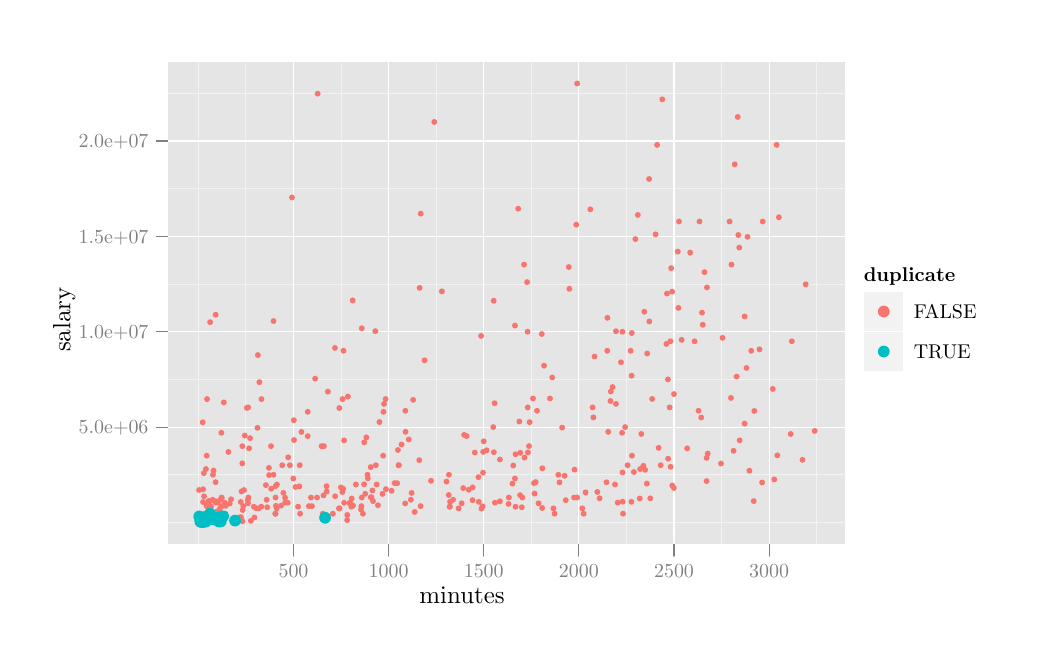
\begin{tikzpicture}[x=1pt,y=1pt]
\draw[color=white,opacity=0] (0,0) rectangle (361.35,216.81);
\begin{scope}
\path[clip] (  0.00,  0.00) rectangle (361.35,216.81);
\definecolor[named]{drawColor}{rgb}{0.31,0.86,0.98}
\end{scope}
\begin{scope}
\path[clip] (  0.00,  0.00) rectangle (361.35,216.81);
\definecolor[named]{drawColor}{rgb}{0.31,0.86,0.98}
\end{scope}
\begin{scope}
\path[clip] (  0.00,  0.00) rectangle (361.35,216.81);
\definecolor[named]{drawColor}{rgb}{0.31,0.86,0.98}
\end{scope}
\begin{scope}
\path[clip] (  0.00,  0.00) rectangle (361.35,216.81);
\definecolor[named]{drawColor}{rgb}{0.31,0.86,0.98}
\end{scope}
\begin{scope}
\path[clip] (  0.00,  0.00) rectangle (361.35,216.81);
\definecolor[named]{drawColor}{rgb}{0.31,0.86,0.98}
\end{scope}
\begin{scope}
\path[clip] (  0.00,  0.00) rectangle (361.35,216.81);
\definecolor[named]{drawColor}{rgb}{0.31,0.86,0.98}
\end{scope}
\begin{scope}
\path[clip] (  0.00,  0.00) rectangle (361.35,216.81);
\definecolor[named]{drawColor}{rgb}{0.31,0.86,0.98}
\end{scope}
\begin{scope}
\path[clip] (  0.00,  0.00) rectangle (361.35,216.81);
\definecolor[named]{drawColor}{rgb}{0.31,0.86,0.98}
\end{scope}
\begin{scope}
\path[clip] (  0.00,  0.00) rectangle (361.35,216.81);
\definecolor[named]{drawColor}{rgb}{0.31,0.86,0.98}
\end{scope}
\begin{scope}
\path[clip] (  0.00,  0.00) rectangle (361.35,216.81);
\definecolor[named]{drawColor}{rgb}{0.31,0.86,0.98}
\end{scope}
\begin{scope}
\path[clip] (  0.00,  0.00) rectangle (361.35,216.81);
\definecolor[named]{drawColor}{rgb}{0.31,0.86,0.98}
\end{scope}
\begin{scope}
\path[clip] (  0.00,  0.00) rectangle (361.35,216.81);
\definecolor[named]{drawColor}{rgb}{0.31,0.86,0.98}
\end{scope}
\begin{scope}
\path[clip] (  0.00,  0.00) rectangle (361.35,216.81);
\definecolor[named]{drawColor}{rgb}{0.31,0.86,0.98}
\end{scope}
\begin{scope}
\path[clip] (  0.00,  0.00) rectangle (361.35,216.81);
\definecolor[named]{drawColor}{rgb}{0.31,0.86,0.98}
\end{scope}
\begin{scope}
\path[clip] (  0.00,  0.00) rectangle (361.35,216.81);
\definecolor[named]{drawColor}{rgb}{0.31,0.86,0.98}
\end{scope}
\begin{scope}
\path[clip] (  0.00,  0.00) rectangle (361.35,216.81);
\definecolor[named]{drawColor}{rgb}{0.31,0.86,0.98}
\end{scope}
\begin{scope}
\path[clip] (  0.00,  0.00) rectangle (361.35,216.81);
\definecolor[named]{drawColor}{rgb}{0.31,0.86,0.98}
\end{scope}
\begin{scope}
\path[clip] (  0.00,  0.00) rectangle (361.35,216.81);
\definecolor[named]{drawColor}{rgb}{0.31,0.86,0.98}
\end{scope}
\begin{scope}
\path[clip] (  0.00,  0.00) rectangle (361.35,216.81);
\definecolor[named]{drawColor}{rgb}{0.31,0.86,0.98}
\end{scope}
\begin{scope}
\path[clip] (  0.00,  0.00) rectangle (361.35,216.81);
\definecolor[named]{drawColor}{rgb}{0.31,0.86,0.98}
\end{scope}
\begin{scope}
\path[clip] (  0.00,  0.00) rectangle (361.35,216.81);
\definecolor[named]{drawColor}{rgb}{0.31,0.86,0.98}
\end{scope}
\begin{scope}
\path[clip] (  0.00,  0.00) rectangle (361.35,216.81);
\definecolor[named]{drawColor}{rgb}{0.31,0.86,0.98}
\end{scope}
\begin{scope}
\path[clip] (  0.00,  0.00) rectangle (361.35,216.81);
\definecolor[named]{drawColor}{rgb}{0.31,0.86,0.98}
\definecolor[named]{fillColor}{rgb}{1.00,1.00,1.00}

\draw[fill=fillColor,draw opacity=0.00,] (  0.00,  0.00) rectangle (361.35,216.81);
\end{scope}
\begin{scope}
\path[clip] (  0.00,  0.00) rectangle (361.35,216.81);
\definecolor[named]{drawColor}{rgb}{0.31,0.86,0.98}
\end{scope}
\begin{scope}
\path[clip] (  0.00,  0.00) rectangle (361.35,216.81);
\definecolor[named]{drawColor}{rgb}{0.31,0.86,0.98}
\end{scope}
\begin{scope}
\path[clip] (  0.00,  0.00) rectangle (361.35,216.81);
\definecolor[named]{drawColor}{rgb}{0.31,0.86,0.98}
\end{scope}
\begin{scope}
\path[clip] (  0.00,  0.00) rectangle (361.35,216.81);
\definecolor[named]{drawColor}{rgb}{0.31,0.86,0.98}
\end{scope}
\begin{scope}
\path[clip] (  0.00,  0.00) rectangle (361.35,216.81);
\definecolor[named]{drawColor}{rgb}{0.31,0.86,0.98}
\end{scope}
\begin{scope}
\path[clip] (  0.00,  0.00) rectangle (361.35,216.81);
\definecolor[named]{drawColor}{rgb}{0.31,0.86,0.98}
\definecolor[named]{drawColor}{rgb}{0.00,0.00,0.00}

\node[color=drawColor,anchor=base,inner sep=0pt, outer sep=0pt, scale=  0.90] at (156.77,  9.03) {minutes%
};
\end{scope}
\begin{scope}
\path[clip] (  0.00,  0.00) rectangle (361.35,216.81);
\definecolor[named]{drawColor}{rgb}{0.31,0.86,0.98}
\end{scope}
\begin{scope}
\path[clip] (  0.00,  0.00) rectangle (361.35,216.81);
\definecolor[named]{drawColor}{rgb}{0.31,0.86,0.98}
\end{scope}
\begin{scope}
\path[clip] (  0.00,  0.00) rectangle (361.35,216.81);
\definecolor[named]{drawColor}{rgb}{0.31,0.86,0.98}
\definecolor[named]{drawColor}{rgb}{0.00,0.00,0.00}

\node[rotate= 90.00,color=drawColor,anchor=base,inner sep=0pt, outer sep=0pt, scale=  0.90] at ( 15.23,111.50) {salary%
};
\end{scope}
\begin{scope}
\path[clip] (  0.00,  0.00) rectangle (361.35,216.81);
\definecolor[named]{drawColor}{rgb}{0.31,0.86,0.98}
\end{scope}
\begin{scope}
\path[clip] (  0.00,  0.00) rectangle (361.35,216.81);
\definecolor[named]{drawColor}{rgb}{0.31,0.86,0.98}
\end{scope}
\begin{scope}
\path[clip] (  0.00,  0.00) rectangle (361.35,216.81);
\definecolor[named]{drawColor}{rgb}{0.31,0.86,0.98}
\end{scope}
\begin{scope}
\path[clip] ( 18.24,204.76) rectangle ( 50.55,204.76);
\definecolor[named]{drawColor}{rgb}{0.31,0.86,0.98}
\end{scope}
\begin{scope}
\path[clip] (  0.00,  0.00) rectangle (361.35,216.81);
\definecolor[named]{drawColor}{rgb}{0.31,0.86,0.98}
\end{scope}
\begin{scope}
\path[clip] ( 18.24,204.76) rectangle ( 50.55,204.76);
\definecolor[named]{drawColor}{rgb}{0.31,0.86,0.98}
\end{scope}
\begin{scope}
\path[clip] (  0.00,  0.00) rectangle (361.35,216.81);
\definecolor[named]{drawColor}{rgb}{0.31,0.86,0.98}
\end{scope}
\begin{scope}
\path[clip] (  0.00,  0.00) rectangle (361.35,216.81);
\definecolor[named]{drawColor}{rgb}{0.31,0.86,0.98}
\end{scope}
\begin{scope}
\path[clip] (  0.00,  0.00) rectangle (361.35,216.81);
\definecolor[named]{drawColor}{rgb}{0.31,0.86,0.98}
\end{scope}
\begin{scope}
\path[clip] ( 18.24, 30.32) rectangle ( 50.55, 30.32);
\definecolor[named]{drawColor}{rgb}{0.31,0.86,0.98}
\end{scope}
\begin{scope}
\path[clip] (  0.00,  0.00) rectangle (361.35,216.81);
\definecolor[named]{drawColor}{rgb}{0.31,0.86,0.98}
\end{scope}
\begin{scope}
\path[clip] ( 18.24, 18.24) rectangle ( 50.55, 30.32);
\definecolor[named]{drawColor}{rgb}{0.31,0.86,0.98}
\end{scope}
\begin{scope}
\path[clip] (  0.00,  0.00) rectangle (361.35,216.81);
\definecolor[named]{drawColor}{rgb}{0.31,0.86,0.98}
\end{scope}
\begin{scope}
\path[clip] ( 18.24, 18.24) rectangle ( 50.55, 18.24);
\definecolor[named]{drawColor}{rgb}{0.31,0.86,0.98}
\end{scope}
\begin{scope}
\path[clip] (  0.00,  0.00) rectangle (361.35,216.81);
\definecolor[named]{drawColor}{rgb}{0.31,0.86,0.98}
\end{scope}
\begin{scope}
\path[clip] ( 50.55,204.76) rectangle ( 50.55,204.76);
\definecolor[named]{drawColor}{rgb}{0.31,0.86,0.98}
\end{scope}
\begin{scope}
\path[clip] (  0.00,  0.00) rectangle (361.35,216.81);
\definecolor[named]{drawColor}{rgb}{0.31,0.86,0.98}
\end{scope}
\begin{scope}
\path[clip] ( 50.55,204.76) rectangle ( 50.55,204.76);
\definecolor[named]{drawColor}{rgb}{0.31,0.86,0.98}
\end{scope}
\begin{scope}
\path[clip] (  0.00,  0.00) rectangle (361.35,216.81);
\definecolor[named]{drawColor}{rgb}{0.31,0.86,0.98}
\end{scope}
\begin{scope}
\path[clip] ( 50.55, 30.32) rectangle ( 50.55,204.77);
\definecolor[named]{drawColor}{rgb}{0.31,0.86,0.98}
\end{scope}
\begin{scope}
\path[clip] (  0.00,  0.00) rectangle (361.35,216.81);
\definecolor[named]{drawColor}{rgb}{0.31,0.86,0.98}
\end{scope}
\begin{scope}
\path[clip] ( 50.55, 30.32) rectangle ( 50.55, 30.32);
\definecolor[named]{drawColor}{rgb}{0.31,0.86,0.98}
\end{scope}
\begin{scope}
\path[clip] (  0.00,  0.00) rectangle (361.35,216.81);
\definecolor[named]{drawColor}{rgb}{0.31,0.86,0.98}
\end{scope}
\begin{scope}
\path[clip] ( 50.55, 18.24) rectangle ( 50.55, 30.32);
\definecolor[named]{drawColor}{rgb}{0.31,0.86,0.98}
\end{scope}
\begin{scope}
\path[clip] (  0.00,  0.00) rectangle (361.35,216.81);
\definecolor[named]{drawColor}{rgb}{0.31,0.86,0.98}
\end{scope}
\begin{scope}
\path[clip] ( 50.55, 18.24) rectangle ( 50.55, 18.24);
\definecolor[named]{drawColor}{rgb}{0.31,0.86,0.98}
\end{scope}
\begin{scope}
\path[clip] (  0.00,  0.00) rectangle (361.35,216.81);
\definecolor[named]{drawColor}{rgb}{0.31,0.86,0.98}
\end{scope}
\begin{scope}
\path[clip] ( 50.55,204.76) rectangle (295.29,204.76);
\definecolor[named]{drawColor}{rgb}{0.31,0.86,0.98}
\end{scope}
\begin{scope}
\path[clip] (  0.00,  0.00) rectangle (361.35,216.81);
\definecolor[named]{drawColor}{rgb}{0.31,0.86,0.98}
\end{scope}
\begin{scope}
\path[clip] ( 50.55,204.76) rectangle (295.29,204.76);
\definecolor[named]{drawColor}{rgb}{0.31,0.86,0.98}
\end{scope}
\begin{scope}
\path[clip] (  0.00,  0.00) rectangle (361.35,216.81);
\definecolor[named]{drawColor}{rgb}{0.31,0.86,0.98}
\end{scope}
\begin{scope}
\path[clip] ( 50.55, 30.32) rectangle (295.29,204.77);
\definecolor[named]{drawColor}{rgb}{0.31,0.86,0.98}
\end{scope}
\begin{scope}
\path[clip] (  0.00,  0.00) rectangle (361.35,216.81);
\definecolor[named]{drawColor}{rgb}{0.31,0.86,0.98}
\end{scope}
\begin{scope}
\path[clip] ( 50.55, 30.32) rectangle (295.29, 30.32);
\definecolor[named]{drawColor}{rgb}{0.31,0.86,0.98}
\end{scope}
\begin{scope}
\path[clip] (  0.00,  0.00) rectangle (361.35,216.81);
\definecolor[named]{drawColor}{rgb}{0.31,0.86,0.98}
\end{scope}
\begin{scope}
\path[clip] (  0.00,  0.00) rectangle (361.35,216.81);
\definecolor[named]{drawColor}{rgb}{0.31,0.86,0.98}
\end{scope}
\begin{scope}
\path[clip] (  0.00,  0.00) rectangle (361.35,216.81);
\definecolor[named]{drawColor}{rgb}{0.31,0.86,0.98}
\end{scope}
\begin{scope}
\path[clip] ( 50.55, 18.24) rectangle (295.29, 18.24);
\definecolor[named]{drawColor}{rgb}{0.31,0.86,0.98}
\end{scope}
\begin{scope}
\path[clip] (  0.00,  0.00) rectangle (361.35,216.81);
\definecolor[named]{drawColor}{rgb}{0.31,0.86,0.98}
\end{scope}
\begin{scope}
\path[clip] (295.29,204.76) rectangle (295.29,204.76);
\definecolor[named]{drawColor}{rgb}{0.31,0.86,0.98}
\end{scope}
\begin{scope}
\path[clip] (  0.00,  0.00) rectangle (361.35,216.81);
\definecolor[named]{drawColor}{rgb}{0.31,0.86,0.98}
\end{scope}
\begin{scope}
\path[clip] (295.29,204.76) rectangle (295.29,204.76);
\definecolor[named]{drawColor}{rgb}{0.31,0.86,0.98}
\end{scope}
\begin{scope}
\path[clip] (  0.00,  0.00) rectangle (361.35,216.81);
\definecolor[named]{drawColor}{rgb}{0.31,0.86,0.98}
\end{scope}
\begin{scope}
\path[clip] (295.29, 30.32) rectangle (295.29,204.77);
\definecolor[named]{drawColor}{rgb}{0.31,0.86,0.98}
\end{scope}
\begin{scope}
\path[clip] (  0.00,  0.00) rectangle (361.35,216.81);
\definecolor[named]{drawColor}{rgb}{0.31,0.86,0.98}
\end{scope}
\begin{scope}
\path[clip] (295.29, 30.32) rectangle (295.29, 30.32);
\definecolor[named]{drawColor}{rgb}{0.31,0.86,0.98}
\end{scope}
\begin{scope}
\path[clip] (  0.00,  0.00) rectangle (361.35,216.81);
\definecolor[named]{drawColor}{rgb}{0.31,0.86,0.98}
\end{scope}
\begin{scope}
\path[clip] (295.29, 18.24) rectangle (295.29, 30.32);
\definecolor[named]{drawColor}{rgb}{0.31,0.86,0.98}
\end{scope}
\begin{scope}
\path[clip] (  0.00,  0.00) rectangle (361.35,216.81);
\definecolor[named]{drawColor}{rgb}{0.31,0.86,0.98}
\end{scope}
\begin{scope}
\path[clip] (295.29, 18.24) rectangle (295.29, 18.24);
\definecolor[named]{drawColor}{rgb}{0.31,0.86,0.98}
\end{scope}
\begin{scope}
\path[clip] (  0.00,  0.00) rectangle (361.35,216.81);
\definecolor[named]{drawColor}{rgb}{0.31,0.86,0.98}
\end{scope}
\begin{scope}
\path[clip] (295.29,204.76) rectangle (295.29,204.76);
\definecolor[named]{drawColor}{rgb}{0.31,0.86,0.98}
\end{scope}
\begin{scope}
\path[clip] (  0.00,  0.00) rectangle (361.35,216.81);
\definecolor[named]{drawColor}{rgb}{0.31,0.86,0.98}
\end{scope}
\begin{scope}
\path[clip] (295.29,204.76) rectangle (295.29,204.76);
\definecolor[named]{drawColor}{rgb}{0.31,0.86,0.98}
\end{scope}
\begin{scope}
\path[clip] (  0.00,  0.00) rectangle (361.35,216.81);
\definecolor[named]{drawColor}{rgb}{0.31,0.86,0.98}
\end{scope}
\begin{scope}
\path[clip] (295.29, 30.32) rectangle (295.29,204.77);
\definecolor[named]{drawColor}{rgb}{0.31,0.86,0.98}
\end{scope}
\begin{scope}
\path[clip] (  0.00,  0.00) rectangle (361.35,216.81);
\definecolor[named]{drawColor}{rgb}{0.31,0.86,0.98}
\end{scope}
\begin{scope}
\path[clip] (295.29, 30.32) rectangle (295.29, 30.32);
\definecolor[named]{drawColor}{rgb}{0.31,0.86,0.98}
\end{scope}
\begin{scope}
\path[clip] (  0.00,  0.00) rectangle (361.35,216.81);
\definecolor[named]{drawColor}{rgb}{0.31,0.86,0.98}
\end{scope}
\begin{scope}
\path[clip] (295.29, 18.24) rectangle (295.29, 30.32);
\definecolor[named]{drawColor}{rgb}{0.31,0.86,0.98}
\end{scope}
\begin{scope}
\path[clip] (  0.00,  0.00) rectangle (361.35,216.81);
\definecolor[named]{drawColor}{rgb}{0.31,0.86,0.98}
\end{scope}
\begin{scope}
\path[clip] (295.29, 18.24) rectangle (295.29, 18.24);
\definecolor[named]{drawColor}{rgb}{0.31,0.86,0.98}
\end{scope}
\begin{scope}
\path[clip] (  0.00,  0.00) rectangle (361.35,216.81);
\definecolor[named]{drawColor}{rgb}{0.31,0.86,0.98}
\end{scope}
\begin{scope}
\path[clip] (295.29,204.76) rectangle (295.29,204.76);
\definecolor[named]{drawColor}{rgb}{0.31,0.86,0.98}
\end{scope}
\begin{scope}
\path[clip] (  0.00,  0.00) rectangle (361.35,216.81);
\definecolor[named]{drawColor}{rgb}{0.31,0.86,0.98}
\end{scope}
\begin{scope}
\path[clip] (295.29,204.76) rectangle (295.29,204.76);
\definecolor[named]{drawColor}{rgb}{0.31,0.86,0.98}
\end{scope}
\begin{scope}
\path[clip] (  0.00,  0.00) rectangle (361.35,216.81);
\definecolor[named]{drawColor}{rgb}{0.31,0.86,0.98}
\end{scope}
\begin{scope}
\path[clip] (295.29, 30.32) rectangle (295.29,204.77);
\definecolor[named]{drawColor}{rgb}{0.31,0.86,0.98}
\end{scope}
\begin{scope}
\path[clip] (  0.00,  0.00) rectangle (361.35,216.81);
\definecolor[named]{drawColor}{rgb}{0.31,0.86,0.98}
\end{scope}
\begin{scope}
\path[clip] (295.29, 30.32) rectangle (295.29, 30.32);
\definecolor[named]{drawColor}{rgb}{0.31,0.86,0.98}
\end{scope}
\begin{scope}
\path[clip] (  0.00,  0.00) rectangle (361.35,216.81);
\definecolor[named]{drawColor}{rgb}{0.31,0.86,0.98}
\end{scope}
\begin{scope}
\path[clip] (295.29, 18.24) rectangle (295.29, 30.32);
\definecolor[named]{drawColor}{rgb}{0.31,0.86,0.98}
\end{scope}
\begin{scope}
\path[clip] (  0.00,  0.00) rectangle (361.35,216.81);
\definecolor[named]{drawColor}{rgb}{0.31,0.86,0.98}
\end{scope}
\begin{scope}
\path[clip] (295.29, 18.24) rectangle (295.29, 18.24);
\definecolor[named]{drawColor}{rgb}{0.31,0.86,0.98}
\end{scope}
\begin{scope}
\path[clip] (  0.00,  0.00) rectangle (361.35,216.81);
\definecolor[named]{drawColor}{rgb}{0.31,0.86,0.98}
\end{scope}
\begin{scope}
\path[clip] ( 18.24,204.76) rectangle ( 50.55,204.76);
\definecolor[named]{drawColor}{rgb}{0.31,0.86,0.98}
\end{scope}
\begin{scope}
\path[clip] (  0.00,  0.00) rectangle (361.35,216.81);
\definecolor[named]{drawColor}{rgb}{0.31,0.86,0.98}
\end{scope}
\begin{scope}
\path[clip] ( 18.24,204.76) rectangle ( 50.55,204.76);
\definecolor[named]{drawColor}{rgb}{0.31,0.86,0.98}
\end{scope}
\begin{scope}
\path[clip] (  0.00,  0.00) rectangle (361.35,216.81);
\definecolor[named]{drawColor}{rgb}{0.31,0.86,0.98}
\end{scope}
\begin{scope}
\path[clip] (  0.00,  0.00) rectangle (361.35,216.81);
\definecolor[named]{drawColor}{rgb}{0.31,0.86,0.98}
\definecolor[named]{drawColor}{rgb}{0.50,0.50,0.50}

\node[color=drawColor,anchor=base east,inner sep=0pt, outer sep=0pt, scale=  0.72] at ( 43.44, 70.20) {5.0e+06%
};

\node[color=drawColor,anchor=base east,inner sep=0pt, outer sep=0pt, scale=  0.72] at ( 43.44,104.66) {1.0e+07%
};

\node[color=drawColor,anchor=base east,inner sep=0pt, outer sep=0pt, scale=  0.72] at ( 43.44,139.12) {1.5e+07%
};

\node[color=drawColor,anchor=base east,inner sep=0pt, outer sep=0pt, scale=  0.72] at ( 43.44,173.57) {2.0e+07%
};
\end{scope}
\begin{scope}
\path[clip] (  0.00,  0.00) rectangle (361.35,216.81);
\definecolor[named]{drawColor}{rgb}{0.31,0.86,0.98}
\definecolor[named]{drawColor}{rgb}{0.50,0.50,0.50}

\draw[color=drawColor,line cap=round,line join=round,fill opacity=0.00,] ( 46.28, 72.68) -- ( 50.55, 72.68);

\draw[color=drawColor,line cap=round,line join=round,fill opacity=0.00,] ( 46.28,107.14) -- ( 50.55,107.14);

\draw[color=drawColor,line cap=round,line join=round,fill opacity=0.00,] ( 46.28,141.60) -- ( 50.55,141.60);

\draw[color=drawColor,line cap=round,line join=round,fill opacity=0.00,] ( 46.28,176.05) -- ( 50.55,176.05);
\end{scope}
\begin{scope}
\path[clip] (  0.00,  0.00) rectangle (361.35,216.81);
\definecolor[named]{drawColor}{rgb}{0.31,0.86,0.98}
\end{scope}
\begin{scope}
\path[clip] (  0.00,  0.00) rectangle (361.35,216.81);
\definecolor[named]{drawColor}{rgb}{0.31,0.86,0.98}
\end{scope}
\begin{scope}
\path[clip] (  0.00,  0.00) rectangle (361.35,216.81);
\definecolor[named]{drawColor}{rgb}{0.31,0.86,0.98}
\end{scope}
\begin{scope}
\path[clip] ( 18.24, 30.32) rectangle ( 50.55, 30.32);
\definecolor[named]{drawColor}{rgb}{0.31,0.86,0.98}
\end{scope}
\begin{scope}
\path[clip] (  0.00,  0.00) rectangle (361.35,216.81);
\definecolor[named]{drawColor}{rgb}{0.31,0.86,0.98}
\end{scope}
\begin{scope}
\path[clip] ( 18.24, 18.24) rectangle ( 50.55, 30.32);
\definecolor[named]{drawColor}{rgb}{0.31,0.86,0.98}
\end{scope}
\begin{scope}
\path[clip] (  0.00,  0.00) rectangle (361.35,216.81);
\definecolor[named]{drawColor}{rgb}{0.31,0.86,0.98}
\end{scope}
\begin{scope}
\path[clip] ( 18.24, 18.24) rectangle ( 50.55, 18.24);
\definecolor[named]{drawColor}{rgb}{0.31,0.86,0.98}
\end{scope}
\begin{scope}
\path[clip] (  0.00,  0.00) rectangle (361.35,216.81);
\definecolor[named]{drawColor}{rgb}{0.31,0.86,0.98}
\end{scope}
\begin{scope}
\path[clip] ( 50.55,204.76) rectangle ( 50.55,204.76);
\definecolor[named]{drawColor}{rgb}{0.31,0.86,0.98}
\end{scope}
\begin{scope}
\path[clip] (  0.00,  0.00) rectangle (361.35,216.81);
\definecolor[named]{drawColor}{rgb}{0.31,0.86,0.98}
\end{scope}
\begin{scope}
\path[clip] ( 50.55,204.76) rectangle ( 50.55,204.76);
\definecolor[named]{drawColor}{rgb}{0.31,0.86,0.98}
\end{scope}
\begin{scope}
\path[clip] (  0.00,  0.00) rectangle (361.35,216.81);
\definecolor[named]{drawColor}{rgb}{0.31,0.86,0.98}
\end{scope}
\begin{scope}
\path[clip] ( 50.55, 30.32) rectangle ( 50.55,204.77);
\definecolor[named]{drawColor}{rgb}{0.31,0.86,0.98}
\end{scope}
\begin{scope}
\path[clip] (  0.00,  0.00) rectangle (361.35,216.81);
\definecolor[named]{drawColor}{rgb}{0.31,0.86,0.98}
\end{scope}
\begin{scope}
\path[clip] ( 50.55, 30.32) rectangle ( 50.55, 30.32);
\definecolor[named]{drawColor}{rgb}{0.31,0.86,0.98}
\end{scope}
\begin{scope}
\path[clip] (  0.00,  0.00) rectangle (361.35,216.81);
\definecolor[named]{drawColor}{rgb}{0.31,0.86,0.98}
\end{scope}
\begin{scope}
\path[clip] ( 50.55, 18.24) rectangle ( 50.55, 30.32);
\definecolor[named]{drawColor}{rgb}{0.31,0.86,0.98}
\end{scope}
\begin{scope}
\path[clip] (  0.00,  0.00) rectangle (361.35,216.81);
\definecolor[named]{drawColor}{rgb}{0.31,0.86,0.98}
\end{scope}
\begin{scope}
\path[clip] ( 50.55, 18.24) rectangle ( 50.55, 18.24);
\definecolor[named]{drawColor}{rgb}{0.31,0.86,0.98}
\end{scope}
\begin{scope}
\path[clip] (  0.00,  0.00) rectangle (361.35,216.81);
\definecolor[named]{drawColor}{rgb}{0.31,0.86,0.98}
\end{scope}
\begin{scope}
\path[clip] ( 50.55,204.76) rectangle (295.29,204.76);
\definecolor[named]{drawColor}{rgb}{0.31,0.86,0.98}
\end{scope}
\begin{scope}
\path[clip] (  0.00,  0.00) rectangle (361.35,216.81);
\definecolor[named]{drawColor}{rgb}{0.31,0.86,0.98}
\end{scope}
\begin{scope}
\path[clip] ( 50.55,204.76) rectangle (295.29,204.76);
\definecolor[named]{drawColor}{rgb}{0.31,0.86,0.98}
\end{scope}
\begin{scope}
\path[clip] (  0.00,  0.00) rectangle (361.35,216.81);
\definecolor[named]{drawColor}{rgb}{0.31,0.86,0.98}
\end{scope}
\begin{scope}
\path[clip] ( 50.55, 30.32) rectangle (295.29,204.77);
\definecolor[named]{drawColor}{rgb}{0.31,0.86,0.98}
\definecolor[named]{fillColor}{rgb}{0.90,0.90,0.90}

\draw[fill=fillColor,draw opacity=0.00,] ( 50.55, 30.32) rectangle (295.29,204.77);
\definecolor[named]{drawColor}{rgb}{0.95,0.95,0.95}

\draw[color=drawColor,line width= 0.0pt,line cap=round,line join=round,fill opacity=0.00,] ( 50.55, 38.23) --
	(295.29, 38.23);

\draw[color=drawColor,line width= 0.0pt,line cap=round,line join=round,fill opacity=0.00,] ( 50.55, 55.45) --
	(295.29, 55.45);

\draw[color=drawColor,line width= 0.0pt,line cap=round,line join=round,fill opacity=0.00,] ( 50.55, 72.68) --
	(295.29, 72.68);

\draw[color=drawColor,line width= 0.0pt,line cap=round,line join=round,fill opacity=0.00,] ( 50.55, 89.91) --
	(295.29, 89.91);

\draw[color=drawColor,line width= 0.0pt,line cap=round,line join=round,fill opacity=0.00,] ( 50.55,107.14) --
	(295.29,107.14);

\draw[color=drawColor,line width= 0.0pt,line cap=round,line join=round,fill opacity=0.00,] ( 50.55,124.37) --
	(295.29,124.37);

\draw[color=drawColor,line width= 0.0pt,line cap=round,line join=round,fill opacity=0.00,] ( 50.55,141.60) --
	(295.29,141.60);

\draw[color=drawColor,line width= 0.0pt,line cap=round,line join=round,fill opacity=0.00,] ( 50.55,158.82) --
	(295.29,158.82);

\draw[color=drawColor,line width= 0.0pt,line cap=round,line join=round,fill opacity=0.00,] ( 50.55,176.05) --
	(295.29,176.05);

\draw[color=drawColor,line width= 0.0pt,line cap=round,line join=round,fill opacity=0.00,] ( 50.55,193.28) --
	(295.29,193.28);

\draw[color=drawColor,line width= 0.0pt,line cap=round,line join=round,fill opacity=0.00,] ( 61.47, 30.32) --
	( 61.47,204.77);

\draw[color=drawColor,line width= 0.0pt,line cap=round,line join=round,fill opacity=0.00,] ( 78.66, 30.32) --
	( 78.66,204.77);

\draw[color=drawColor,line width= 0.0pt,line cap=round,line join=round,fill opacity=0.00,] ( 95.85, 30.32) --
	( 95.85,204.77);

\draw[color=drawColor,line width= 0.0pt,line cap=round,line join=round,fill opacity=0.00,] (113.04, 30.32) --
	(113.04,204.77);

\draw[color=drawColor,line width= 0.0pt,line cap=round,line join=round,fill opacity=0.00,] (130.22, 30.32) --
	(130.22,204.77);

\draw[color=drawColor,line width= 0.0pt,line cap=round,line join=round,fill opacity=0.00,] (147.41, 30.32) --
	(147.41,204.77);

\draw[color=drawColor,line width= 0.0pt,line cap=round,line join=round,fill opacity=0.00,] (164.60, 30.32) --
	(164.60,204.77);

\draw[color=drawColor,line width= 0.0pt,line cap=round,line join=round,fill opacity=0.00,] (181.79, 30.32) --
	(181.79,204.77);

\draw[color=drawColor,line width= 0.0pt,line cap=round,line join=round,fill opacity=0.00,] (198.98, 30.32) --
	(198.98,204.77);

\draw[color=drawColor,line width= 0.0pt,line cap=round,line join=round,fill opacity=0.00,] (216.17, 30.32) --
	(216.17,204.77);

\draw[color=drawColor,line width= 0.0pt,line cap=round,line join=round,fill opacity=0.00,] (233.36, 30.32) --
	(233.36,204.77);

\draw[color=drawColor,line width= 0.0pt,line cap=round,line join=round,fill opacity=0.00,] (250.55, 30.32) --
	(250.55,204.77);

\draw[color=drawColor,line width= 0.0pt,line cap=round,line join=round,fill opacity=0.00,] (267.74, 30.32) --
	(267.74,204.77);

\draw[color=drawColor,line width= 0.0pt,line cap=round,line join=round,fill opacity=0.00,] (284.93, 30.32) --
	(284.93,204.77);
\definecolor[named]{drawColor}{rgb}{1.00,1.00,1.00}

\draw[color=drawColor,line cap=round,line join=round,fill opacity=0.00,] ( 50.55, 72.68) --
	(295.29, 72.68);

\draw[color=drawColor,line cap=round,line join=round,fill opacity=0.00,] ( 50.55,107.14) --
	(295.29,107.14);

\draw[color=drawColor,line cap=round,line join=round,fill opacity=0.00,] ( 50.55,141.60) --
	(295.29,141.60);

\draw[color=drawColor,line cap=round,line join=round,fill opacity=0.00,] ( 50.55,176.05) --
	(295.29,176.05);

\draw[color=drawColor,line cap=round,line join=round,fill opacity=0.00,] ( 95.85, 30.32) --
	( 95.85,204.77);

\draw[color=drawColor,line cap=round,line join=round,fill opacity=0.00,] (130.22, 30.32) --
	(130.22,204.77);

\draw[color=drawColor,line cap=round,line join=round,fill opacity=0.00,] (164.60, 30.32) --
	(164.60,204.77);

\draw[color=drawColor,line cap=round,line join=round,fill opacity=0.00,] (198.98, 30.32) --
	(198.98,204.77);

\draw[color=drawColor,line cap=round,line join=round,fill opacity=0.00,] (233.36, 30.32) --
	(233.36,204.77);

\draw[color=drawColor,line cap=round,line join=round,fill opacity=0.00,] (267.74, 30.32) --
	(267.74,204.77);
\definecolor[named]{fillColor}{rgb}{0.97,0.46,0.43}

\draw[fill=fillColor,draw opacity=0.00,] (214.79, 45.71) circle (  1.07);

\draw[fill=fillColor,draw opacity=0.00,] ( 63.53, 47.68) circle (  1.07);

\draw[fill=fillColor,draw opacity=0.00,] (262.37, 78.50) circle (  1.07);

\draw[fill=fillColor,draw opacity=0.00,] ( 63.46, 56.03) circle (  1.07);

\draw[fill=fillColor,draw opacity=0.00,] ( 92.82, 47.19) circle (  1.07);

\draw[fill=fillColor,draw opacity=0.00,] (255.29,167.62) circle (  1.07);

\draw[fill=fillColor,draw opacity=0.00,] (122.59, 55.45) circle (  1.07);

\draw[fill=fillColor,draw opacity=0.00,] (114.14, 67.86) circle (  1.07);

\draw[fill=fillColor,draw opacity=0.00,] (141.78, 44.12) circle (  1.07);

\draw[fill=fillColor,draw opacity=0.00,] ( 62.50, 38.60) circle (  1.07);

\draw[fill=fillColor,draw opacity=0.00,] (177.80, 63.38) circle (  1.07);

\draw[fill=fillColor,draw opacity=0.00,] (122.73, 54.18) circle (  1.07);

\draw[fill=fillColor,draw opacity=0.00,] (124.04, 47.30) circle (  1.07);

\draw[fill=fillColor,draw opacity=0.00,] (242.57,146.97) circle (  1.07);

\draw[fill=fillColor,draw opacity=0.00,] (152.36, 43.92) circle (  1.07);

\draw[fill=fillColor,draw opacity=0.00,] (141.84,149.81) circle (  1.07);

\draw[fill=fillColor,draw opacity=0.00,] (242.23, 78.57) circle (  1.07);

\draw[fill=fillColor,draw opacity=0.00,] ( 64.22, 57.53) circle (  1.07);

\draw[fill=fillColor,draw opacity=0.00,] (170.45, 45.86) circle (  1.07);

\draw[fill=fillColor,draw opacity=0.00,] ( 92.89, 45.47) circle (  1.07);

\draw[fill=fillColor,draw opacity=0.00,] (162.68, 54.59) circle (  1.07);

\draw[fill=fillColor,draw opacity=0.00,] ( 77.35, 59.59) circle (  1.07);

\draw[fill=fillColor,draw opacity=0.00,] ( 67.73, 52.78) circle (  1.07);

\draw[fill=fillColor,draw opacity=0.00,] ( 78.25, 69.61) circle (  1.07);

\draw[fill=fillColor,draw opacity=0.00,] (115.51, 83.71) circle (  1.07);

\draw[fill=fillColor,draw opacity=0.00,] (253.92, 83.21) circle (  1.07);

\draw[fill=fillColor,draw opacity=0.00,] (205.65, 49.25) circle (  1.07);

\draw[fill=fillColor,draw opacity=0.00,] ( 77.42, 38.68) circle (  1.07);

\draw[fill=fillColor,draw opacity=0.00,] (106.02, 65.79) circle (  1.07);

\draw[fill=fillColor,draw opacity=0.00,] (210.53, 85.53) circle (  1.07);

\draw[fill=fillColor,draw opacity=0.00,] ( 70.68, 81.59) circle (  1.07);

\draw[fill=fillColor,draw opacity=0.00,] (124.59, 45.94) circle (  1.07);

\draw[fill=fillColor,draw opacity=0.00,] (151.13, 52.99) circle (  1.07);

\draw[fill=fillColor,draw opacity=0.00,] (221.53, 70.19) circle (  1.07);

\draw[fill=fillColor,draw opacity=0.00,] (138.54, 48.89) circle (  1.07);

\draw[fill=fillColor,draw opacity=0.00,] ( 63.05, 74.41) circle (  1.07);

\draw[fill=fillColor,draw opacity=0.00,] ( 81.55, 43.91) circle (  1.07);

\draw[fill=fillColor,draw opacity=0.00,] (212.39, 81.07) circle (  1.07);

\draw[fill=fillColor,draw opacity=0.00,] (113.93,100.25) circle (  1.07);

\draw[fill=fillColor,draw opacity=0.00,] (232.67,121.61) circle (  1.07);

\draw[fill=fillColor,draw opacity=0.00,] (164.19, 44.08) circle (  1.07);

\draw[fill=fillColor,draw opacity=0.00,] (157.52, 69.86) circle (  1.07);

\draw[fill=fillColor,draw opacity=0.00,] (216.58, 58.90) circle (  1.07);

\draw[fill=fillColor,draw opacity=0.00,] (168.66, 45.35) circle (  1.07);

\draw[fill=fillColor,draw opacity=0.00,] (214.73,107.14) circle (  1.07);

\draw[fill=fillColor,draw opacity=0.00,] (141.29, 60.74) circle (  1.07);

\draw[fill=fillColor,draw opacity=0.00,] (133.32, 52.40) circle (  1.07);

\draw[fill=fillColor,draw opacity=0.00,] (245.25,123.15) circle (  1.07);

\draw[fill=fillColor,draw opacity=0.00,] (235.15,146.97) circle (  1.07);

\draw[fill=fillColor,draw opacity=0.00,] ( 62.02, 39.67) circle (  1.07);

\draw[fill=fillColor,draw opacity=0.00,] (138.27, 46.44) circle (  1.07);

\draw[fill=fillColor,draw opacity=0.00,] (219.40,140.62) circle (  1.07);

\draw[fill=fillColor,draw opacity=0.00,] (232.12, 58.32) circle (  1.07);

\draw[fill=fillColor,draw opacity=0.00,] ( 66.97, 56.95) circle (  1.07);

\draw[fill=fillColor,draw opacity=0.00,] ( 65.53, 45.86) circle (  1.07);

\draw[fill=fillColor,draw opacity=0.00,] (106.44, 41.38) circle (  1.07);

\draw[fill=fillColor,draw opacity=0.00,] (262.17, 45.93) circle (  1.07);

\draw[fill=fillColor,draw opacity=0.00,] ( 67.86, 45.86) circle (  1.07);

\draw[fill=fillColor,draw opacity=0.00,] ( 98.25, 41.38) circle (  1.07);

\draw[fill=fillColor,draw opacity=0.00,] (106.85, 65.79) circle (  1.07);

\draw[fill=fillColor,draw opacity=0.00,] (178.35, 43.72) circle (  1.07);

\draw[fill=fillColor,draw opacity=0.00,] (256.39,184.75) circle (  1.07);

\draw[fill=fillColor,draw opacity=0.00,] (163.78, 43.22) circle (  1.07);

\draw[fill=fillColor,draw opacity=0.00,] (125.41,107.35) circle (  1.07);

\draw[fill=fillColor,draw opacity=0.00,] (197.40, 57.31) circle (  1.07);

\draw[fill=fillColor,draw opacity=0.00,] (176.08, 43.92) circle (  1.07);

\draw[fill=fillColor,draw opacity=0.00,] (186.40, 94.87) circle (  1.07);

\draw[fill=fillColor,draw opacity=0.00,] (110.84,101.28) circle (  1.07);

\draw[fill=fillColor,draw opacity=0.00,] (120.39, 44.12) circle (  1.07);

\draw[fill=fillColor,draw opacity=0.00,] (116.13, 45.18) circle (  1.07);

\draw[fill=fillColor,draw opacity=0.00,] ( 69.79, 70.62) circle (  1.07);

\draw[fill=fillColor,draw opacity=0.00,] (120.53, 47.23) circle (  1.07);

\draw[fill=fillColor,draw opacity=0.00,] (220.29,149.34) circle (  1.07);

\draw[fill=fillColor,draw opacity=0.00,] (194.24, 46.27) circle (  1.07);

\draw[fill=fillColor,draw opacity=0.00,] (185.71, 43.44) circle (  1.07);

\draw[fill=fillColor,draw opacity=0.00,] (141.43,122.99) circle (  1.07);

\draw[fill=fillColor,draw opacity=0.00,] (220.98, 46.88) circle (  1.07);

\draw[fill=fillColor,draw opacity=0.00,] ( 87.80, 50.40) circle (  1.07);

\draw[fill=fillColor,draw opacity=0.00,] (206.47, 46.95) circle (  1.07);

\draw[fill=fillColor,draw opacity=0.00,] ( 69.38, 46.37) circle (  1.07);

\draw[fill=fillColor,draw opacity=0.00,] ( 79.35, 46.37) circle (  1.07);

\draw[fill=fillColor,draw opacity=0.00,] ( 93.78, 45.36) circle (  1.07);

\draw[fill=fillColor,draw opacity=0.00,] (168.52, 81.30) circle (  1.07);

\draw[fill=fillColor,draw opacity=0.00,] (238.10, 64.99) circle (  1.07);

\draw[fill=fillColor,draw opacity=0.00,] ( 63.94, 38.82) circle (  1.07);

\draw[fill=fillColor,draw opacity=0.00,] ( 64.49, 62.35) circle (  1.07);

\draw[fill=fillColor,draw opacity=0.00,] (230.61,102.73) circle (  1.07);

\draw[fill=fillColor,draw opacity=0.00,] (110.08, 41.38) circle (  1.07);

\draw[fill=fillColor,draw opacity=0.00,] ( 65.73,110.59) circle (  1.07);

\draw[fill=fillColor,draw opacity=0.00,] (260.59, 56.91) circle (  1.07);

\draw[fill=fillColor,draw opacity=0.00,] (149.48,121.72) circle (  1.07);

\draw[fill=fillColor,draw opacity=0.00,] (125.89, 51.94) circle (  1.07);

\draw[fill=fillColor,draw opacity=0.00,] (234.94,115.75) circle (  1.07);

\draw[fill=fillColor,draw opacity=0.00,] (125.62, 58.90) circle (  1.07);

\draw[fill=fillColor,draw opacity=0.00,] ( 62.02, 38.78) circle (  1.07);

\draw[fill=fillColor,draw opacity=0.00,] ( 95.78, 54.08) circle (  1.07);

\draw[fill=fillColor,draw opacity=0.00,] (124.38, 49.79) circle (  1.07);

\draw[fill=fillColor,draw opacity=0.00,] (218.16, 62.35) circle (  1.07);

\draw[fill=fillColor,draw opacity=0.00,] (243.74,109.65) circle (  1.07);

\draw[fill=fillColor,draw opacity=0.00,] (175.88, 54.11) circle (  1.07);

\draw[fill=fillColor,draw opacity=0.00,] ( 64.49, 44.33) circle (  1.07);

\draw[fill=fillColor,draw opacity=0.00,] (261.27,100.25) circle (  1.07);

\draw[fill=fillColor,draw opacity=0.00,] ( 63.19, 50.22) circle (  1.07);

\draw[fill=fillColor,draw opacity=0.00,] ( 79.48, 79.79) circle (  1.07);

\draw[fill=fillColor,draw opacity=0.00,] (128.23, 62.35) circle (  1.07);

\draw[fill=fillColor,draw opacity=0.00,] (136.21, 45.09) circle (  1.07);

\draw[fill=fillColor,draw opacity=0.00,] (160.61, 50.88) circle (  1.07);

\draw[fill=fillColor,draw opacity=0.00,] (198.36, 47.24) circle (  1.07);

\draw[fill=fillColor,draw opacity=0.00,] (203.93, 79.79) circle (  1.07);

\draw[fill=fillColor,draw opacity=0.00,] (229.10,191.10) circle (  1.07);

\draw[fill=fillColor,draw opacity=0.00,] (163.64,105.63) circle (  1.07);

\draw[fill=fillColor,draw opacity=0.00,] (284.17, 71.28) circle (  1.07);

\draw[fill=fillColor,draw opacity=0.00,] (156.63, 45.14) circle (  1.07);

\draw[fill=fillColor,draw opacity=0.00,] (243.47,114.03) circle (  1.07);

\draw[fill=fillColor,draw opacity=0.00,] ( 61.74, 49.94) circle (  1.07);

\draw[fill=fillColor,draw opacity=0.00,] (152.02, 55.45) circle (  1.07);

\draw[fill=fillColor,draw opacity=0.00,] ( 82.85, 72.41) circle (  1.07);

\draw[fill=fillColor,draw opacity=0.00,] (245.53, 63.10) circle (  1.07);

\draw[fill=fillColor,draw opacity=0.00,] (162.81, 45.67) circle (  1.07);

\draw[fill=fillColor,draw opacity=0.00,] (243.19, 76.14) circle (  1.07);

\draw[fill=fillColor,draw opacity=0.00,] (160.55, 46.26) circle (  1.07);

\draw[fill=fillColor,draw opacity=0.00,] ( 89.52, 44.22) circle (  1.07);

\draw[fill=fillColor,draw opacity=0.00,] ( 88.63, 55.45) circle (  1.07);

\draw[fill=fillColor,draw opacity=0.00,] (214.59, 70.62) circle (  1.07);

\draw[fill=fillColor,draw opacity=0.00,] (222.29, 58.69) circle (  1.07);

\draw[fill=fillColor,draw opacity=0.00,] (143.22, 96.80) circle (  1.07);

\draw[fill=fillColor,draw opacity=0.00,] ( 79.00, 79.63) circle (  1.07);

\draw[fill=fillColor,draw opacity=0.00,] (176.08, 62.87) circle (  1.07);

\draw[fill=fillColor,draw opacity=0.00,] (212.04, 51.94) circle (  1.07);

\draw[fill=fillColor,draw opacity=0.00,] ( 76.39, 40.10) circle (  1.07);

\draw[fill=fillColor,draw opacity=0.00,] (250.34, 59.51) circle (  1.07);

\draw[fill=fillColor,draw opacity=0.00,] (101.00, 78.20) circle (  1.07);

\draw[fill=fillColor,draw opacity=0.00,] (203.11,151.36) circle (  1.07);

\draw[fill=fillColor,draw opacity=0.00,] (231.23, 61.25) circle (  1.07);

\draw[fill=fillColor,draw opacity=0.00,] (226.69,142.33) circle (  1.07);

\draw[fill=fillColor,draw opacity=0.00,] (279.77, 60.84) circle (  1.07);

\draw[fill=fillColor,draw opacity=0.00,] ( 73.98, 38.60) circle (  1.07);

\draw[fill=fillColor,draw opacity=0.00,] (113.79, 50.41) circle (  1.07);

\draw[fill=fillColor,draw opacity=0.00,] (134.90, 66.40) circle (  1.07);

\draw[fill=fillColor,draw opacity=0.00,] (213.01, 45.39) circle (  1.07);

\draw[fill=fillColor,draw opacity=0.00,] ( 71.09, 45.32) circle (  1.07);

\draw[fill=fillColor,draw opacity=0.00,] ( 61.81, 38.41) circle (  1.07);

\draw[fill=fillColor,draw opacity=0.00,] (209.29,112.16) circle (  1.07);

\draw[fill=fillColor,draw opacity=0.00,] (180.42,107.14) circle (  1.07);

\draw[fill=fillColor,draw opacity=0.00,] (214.73, 56.30) circle (  1.07);

\draw[fill=fillColor,draw opacity=0.00,] (136.28, 78.57) circle (  1.07);

\draw[fill=fillColor,draw opacity=0.00,] (116.75, 43.92) circle (  1.07);

\draw[fill=fillColor,draw opacity=0.00,] (218.09,106.66) circle (  1.07);

\draw[fill=fillColor,draw opacity=0.00,] ( 79.41, 45.12) circle (  1.07);

\draw[fill=fillColor,draw opacity=0.00,] ( 69.38, 41.38) circle (  1.07);

\draw[fill=fillColor,draw opacity=0.00,] (173.54, 44.92) circle (  1.07);

\draw[fill=fillColor,draw opacity=0.00,] (270.69, 62.46) circle (  1.07);

\draw[fill=fillColor,draw opacity=0.00,] (168.25, 63.60) circle (  1.07);

\draw[fill=fillColor,draw opacity=0.00,] ( 63.67, 41.38) circle (  1.07);

\draw[fill=fillColor,draw opacity=0.00,] ( 77.97, 49.93) circle (  1.07);

\draw[fill=fillColor,draw opacity=0.00,] ( 83.26, 43.30) circle (  1.07);

\draw[fill=fillColor,draw opacity=0.00,] ( 64.49, 44.12) circle (  1.07);

\draw[fill=fillColor,draw opacity=0.00,] (168.18,118.34) circle (  1.07);

\draw[fill=fillColor,draw opacity=0.00,] ( 96.60, 51.04) circle (  1.07);

\draw[fill=fillColor,draw opacity=0.00,] (180.97, 65.82) circle (  1.07);

\draw[fill=fillColor,draw opacity=0.00,] (212.39,107.32) circle (  1.07);

\draw[fill=fillColor,draw opacity=0.00,] (214.18, 96.11) circle (  1.07);

\draw[fill=fillColor,draw opacity=0.00,] (211.15, 87.15) circle (  1.07);

\draw[fill=fillColor,draw opacity=0.00,] (137.51, 68.20) circle (  1.07);

\draw[fill=fillColor,draw opacity=0.00,] (183.37, 52.82) circle (  1.07);

\draw[fill=fillColor,draw opacity=0.00,] (132.42, 52.44) circle (  1.07);

\draw[fill=fillColor,draw opacity=0.00,] (112.42, 79.57) circle (  1.07);

\draw[fill=fillColor,draw opacity=0.00,] (117.37, 44.32) circle (  1.07);

\draw[fill=fillColor,draw opacity=0.00,] ( 85.88, 51.71) circle (  1.07);

\draw[fill=fillColor,draw opacity=0.00,] (201.39, 49.08) circle (  1.07);

\draw[fill=fillColor,draw opacity=0.00,] (177.73, 48.08) circle (  1.07);

\draw[fill=fillColor,draw opacity=0.00,] (250.89,104.93) circle (  1.07);

\draw[fill=fillColor,draw opacity=0.00,] (217.96, 45.68) circle (  1.07);

\draw[fill=fillColor,draw opacity=0.00,] (228.55, 58.90) circle (  1.07);

\draw[fill=fillColor,draw opacity=0.00,] ( 87.05, 55.34) circle (  1.07);

\draw[fill=fillColor,draw opacity=0.00,] (232.05,103.69) circle (  1.07);

\draw[fill=fillColor,draw opacity=0.00,] (182.96, 48.66) circle (  1.07);

\draw[fill=fillColor,draw opacity=0.00,] (145.56, 53.27) circle (  1.07);

\draw[fill=fillColor,draw opacity=0.00,] (257.08, 67.91) circle (  1.07);

\draw[fill=fillColor,draw opacity=0.00,] ( 86.98, 57.95) circle (  1.07);

\draw[fill=fillColor,draw opacity=0.00,] (256.94,137.53) circle (  1.07);

\draw[fill=fillColor,draw opacity=0.00,] ( 67.73,113.27) circle (  1.07);

\draw[fill=fillColor,draw opacity=0.00,] (173.68, 47.23) circle (  1.07);

\draw[fill=fillColor,draw opacity=0.00,] ( 81.75, 40.03) circle (  1.07);

\draw[fill=fillColor,draw opacity=0.00,] (123.76, 58.21) circle (  1.07);

\draw[fill=fillColor,draw opacity=0.00,] (115.30, 40.93) circle (  1.07);

\draw[fill=fillColor,draw opacity=0.00,] ( 69.86, 47.23) circle (  1.07);

\draw[fill=fillColor,draw opacity=0.00,] ( 63.74, 40.50) circle (  1.07);

\draw[fill=fillColor,draw opacity=0.00,] ( 72.33, 63.70) circle (  1.07);

\draw[fill=fillColor,draw opacity=0.00,] (152.43, 45.70) circle (  1.07);

\draw[fill=fillColor,draw opacity=0.00,] (280.94,124.27) circle (  1.07);

\draw[fill=fillColor,draw opacity=0.00,] (153.53, 46.43) circle (  1.07);

\draw[fill=fillColor,draw opacity=0.00,] (191.97, 52.70) circle (  1.07);

\draw[fill=fillColor,draw opacity=0.00,] (116.34, 45.32) circle (  1.07);

\draw[fill=fillColor,draw opacity=0.00,] ( 67.66, 45.46) circle (  1.07);

\draw[fill=fillColor,draw opacity=0.00,] (215.69, 72.68) circle (  1.07);

\draw[fill=fillColor,draw opacity=0.00,] ( 69.31, 43.30) circle (  1.07);

\draw[fill=fillColor,draw opacity=0.00,] (255.98, 90.94) circle (  1.07);

\draw[fill=fillColor,draw opacity=0.00,] (265.40,146.97) circle (  1.07);

\draw[fill=fillColor,draw opacity=0.00,] ( 64.63, 82.79) circle (  1.07);

\draw[fill=fillColor,draw opacity=0.00,] (117.23,118.45) circle (  1.07);

\draw[fill=fillColor,draw opacity=0.00,] ( 89.80, 43.30) circle (  1.07);

\draw[fill=fillColor,draw opacity=0.00,] (230.81,120.92) circle (  1.07);

\draw[fill=fillColor,draw opacity=0.00,] ( 66.42, 39.02) circle (  1.07);

\draw[fill=fillColor,draw opacity=0.00,] (234.73,136.08) circle (  1.07);

\draw[fill=fillColor,draw opacity=0.00,] ( 84.30, 82.79) circle (  1.07);

\draw[fill=fillColor,draw opacity=0.00,] (245.12, 53.17) circle (  1.07);

\draw[fill=fillColor,draw opacity=0.00,] (214.93, 41.38) circle (  1.07);

\draw[fill=fillColor,draw opacity=0.00,] (175.26, 58.80) circle (  1.07);

\draw[fill=fillColor,draw opacity=0.00,] (161.37, 63.49) circle (  1.07);

\draw[fill=fillColor,draw opacity=0.00,] ( 89.38, 51.32) circle (  1.07);

\draw[fill=fillColor,draw opacity=0.00,] (113.52, 49.21) circle (  1.07);

\draw[fill=fillColor,draw opacity=0.00,] (259.90,141.43) circle (  1.07);

\draw[fill=fillColor,draw opacity=0.00,] (191.55, 55.45) circle (  1.07);

\draw[fill=fillColor,draw opacity=0.00,] ( 61.95, 38.59) circle (  1.07);

\draw[fill=fillColor,draw opacity=0.00,] ( 96.05, 68.00) circle (  1.07);

\draw[fill=fillColor,draw opacity=0.00,] (107.88, 49.39) circle (  1.07);

\draw[fill=fillColor,draw opacity=0.00,] (139.64, 42.02) circle (  1.07);

\draw[fill=fillColor,draw opacity=0.00,] (240.78,103.69) circle (  1.07);

\draw[fill=fillColor,draw opacity=0.00,] (128.57, 81.04) circle (  1.07);

\draw[fill=fillColor,draw opacity=0.00,] (259.55, 94.05) circle (  1.07);

\draw[fill=fillColor,draw opacity=0.00,] (177.05,151.60) circle (  1.07);

\draw[fill=fillColor,draw opacity=0.00,] (126.92, 74.50) circle (  1.07);

\draw[fill=fillColor,draw opacity=0.00,] ( 73.29, 46.59) circle (  1.07);

\draw[fill=fillColor,draw opacity=0.00,] (181.17, 74.45) circle (  1.07);

\draw[fill=fillColor,draw opacity=0.00,] ( 62.98, 38.24) circle (  1.07);

\draw[fill=fillColor,draw opacity=0.00,] (133.94, 58.90) circle (  1.07);

\draw[fill=fillColor,draw opacity=0.00,] ( 61.68, 41.38) circle (  1.07);

\draw[fill=fillColor,draw opacity=0.00,] (151.95, 48.14) circle (  1.07);

\draw[fill=fillColor,draw opacity=0.00,] (224.76, 46.94) circle (  1.07);

\draw[fill=fillColor,draw opacity=0.00,] (269.04, 86.47) circle (  1.07);

\draw[fill=fillColor,draw opacity=0.00,] (224.35,162.34) circle (  1.07);

\draw[fill=fillColor,draw opacity=0.00,] (269.59, 53.77) circle (  1.07);

\draw[fill=fillColor,draw opacity=0.00,] (129.26, 50.26) circle (  1.07);

\draw[fill=fillColor,draw opacity=0.00,] (179.32, 61.66) circle (  1.07);

\draw[fill=fillColor,draw opacity=0.00,] (174.98, 52.25) circle (  1.07);

\draw[fill=fillColor,draw opacity=0.00,] ( 86.15, 46.41) circle (  1.07);

\draw[fill=fillColor,draw opacity=0.00,] ( 72.81, 45.05) circle (  1.07);

\draw[fill=fillColor,draw opacity=0.00,] (225.45, 82.85) circle (  1.07);

\draw[fill=fillColor,draw opacity=0.00,] ( 66.63, 46.41) circle (  1.07);

\draw[fill=fillColor,draw opacity=0.00,] ( 80.45, 38.82) circle (  1.07);

\draw[fill=fillColor,draw opacity=0.00,] (198.02,145.82) circle (  1.07);

\draw[fill=fillColor,draw opacity=0.00,] (120.53,108.38) circle (  1.07);

\draw[fill=fillColor,draw opacity=0.00,] ( 66.01, 38.71) circle (  1.07);

\draw[fill=fillColor,draw opacity=0.00,] (165.63, 64.28) circle (  1.07);

\draw[fill=fillColor,draw opacity=0.00,] (200.70, 41.38) circle (  1.07);

\draw[fill=fillColor,draw opacity=0.00,] (168.04, 72.68) circle (  1.07);

\draw[fill=fillColor,draw opacity=0.00,] (123.76, 47.32) circle (  1.07);

\draw[fill=fillColor,draw opacity=0.00,] (275.51, 70.19) circle (  1.07);

\draw[fill=fillColor,draw opacity=0.00,] ( 84.23, 43.92) circle (  1.07);

\draw[fill=fillColor,draw opacity=0.00,] (189.77, 43.30) circle (  1.07);

\draw[fill=fillColor,draw opacity=0.00,] (128.02, 48.54) circle (  1.07);

\draw[fill=fillColor,draw opacity=0.00,] (104.58,193.16) circle (  1.07);

\draw[fill=fillColor,draw opacity=0.00,] ( 66.08, 43.92) circle (  1.07);

\draw[fill=fillColor,draw opacity=0.00,] ( 97.50, 43.92) circle (  1.07);

\draw[fill=fillColor,draw opacity=0.00,] ( 77.49, 42.71) circle (  1.07);

\draw[fill=fillColor,draw opacity=0.00,] (164.40, 63.72) circle (  1.07);

\draw[fill=fillColor,draw opacity=0.00,] (103.68, 90.19) circle (  1.07);

\draw[fill=fillColor,draw opacity=0.00,] (233.36, 84.61) circle (  1.07);

\draw[fill=fillColor,draw opacity=0.00,] (195.54,122.64) circle (  1.07);

\draw[fill=fillColor,draw opacity=0.00,] (185.57,106.32) circle (  1.07);

\draw[fill=fillColor,draw opacity=0.00,] (218.03, 91.24) circle (  1.07);

\draw[fill=fillColor,draw opacity=0.00,] ( 64.08, 41.38) circle (  1.07);

\draw[fill=fillColor,draw opacity=0.00,] (129.12, 82.79) circle (  1.07);

\draw[fill=fillColor,draw opacity=0.00,] (133.80, 58.90) circle (  1.07);

\draw[fill=fillColor,draw opacity=0.00,] ( 89.38, 47.23) circle (  1.07);

\draw[fill=fillColor,draw opacity=0.00,] ( 69.99, 44.12) circle (  1.07);

\draw[fill=fillColor,draw opacity=0.00,] (200.22, 43.30) circle (  1.07);

\draw[fill=fillColor,draw opacity=0.00,] ( 65.18, 45.95) circle (  1.07);

\draw[fill=fillColor,draw opacity=0.00,] (222.63,114.36) circle (  1.07);

\draw[fill=fillColor,draw opacity=0.00,] ( 94.54, 58.90) circle (  1.07);

\draw[fill=fillColor,draw opacity=0.00,] (244.36,128.67) circle (  1.07);

\draw[fill=fillColor,draw opacity=0.00,] (189.35, 90.60) circle (  1.07);

\draw[fill=fillColor,draw opacity=0.00,] ( 89.87, 51.94) circle (  1.07);

\draw[fill=fillColor,draw opacity=0.00,] (193.82, 55.08) circle (  1.07);

\draw[fill=fillColor,draw opacity=0.00,] ( 86.36, 43.72) circle (  1.07);

\draw[fill=fillColor,draw opacity=0.00,] (270.42,174.64) circle (  1.07);

\draw[fill=fillColor,draw opacity=0.00,] ( 64.98, 44.12) circle (  1.07);

\draw[fill=fillColor,draw opacity=0.00,] ( 95.98, 75.17) circle (  1.07);

\draw[fill=fillColor,draw opacity=0.00,] (239.20,135.73) circle (  1.07);

\draw[fill=fillColor,draw opacity=0.00,] (224.42,110.85) circle (  1.07);

\draw[fill=fillColor,draw opacity=0.00,] (209.23,100.25) circle (  1.07);

\draw[fill=fillColor,draw opacity=0.00,] ( 79.55, 47.23) circle (  1.07);

\draw[fill=fillColor,draw opacity=0.00,] (198.36,196.84) circle (  1.07);

\draw[fill=fillColor,draw opacity=0.00,] (146.73,182.94) circle (  1.07);

\draw[fill=fillColor,draw opacity=0.00,] ( 77.35, 65.79) circle (  1.07);

\draw[fill=fillColor,draw opacity=0.00,] (136.34, 70.96) circle (  1.07);

\draw[fill=fillColor,draw opacity=0.00,] (118.40, 51.94) circle (  1.07);

\draw[fill=fillColor,draw opacity=0.00,] (218.85, 56.45) circle (  1.07);

\draw[fill=fillColor,draw opacity=0.00,] (180.28,125.06) circle (  1.07);

\draw[fill=fillColor,draw opacity=0.00,] (179.18,131.40) circle (  1.07);

\draw[fill=fillColor,draw opacity=0.00,] (121.77, 48.56) circle (  1.07);

\draw[fill=fillColor,draw opacity=0.00,] ( 92.20, 48.89) circle (  1.07);

\draw[fill=fillColor,draw opacity=0.00,] ( 89.32, 41.38) circle (  1.07);

\draw[fill=fillColor,draw opacity=0.00,] (209.57, 70.96) circle (  1.07);

\draw[fill=fillColor,draw opacity=0.00,] (128.37, 78.20) circle (  1.07);

\draw[fill=fillColor,draw opacity=0.00,] ( 91.38, 44.32) circle (  1.07);

\draw[fill=fillColor,draw opacity=0.00,] (227.24,174.64) circle (  1.07);

\draw[fill=fillColor,draw opacity=0.00,] (177.46, 74.69) circle (  1.07);

\draw[fill=fillColor,draw opacity=0.00,] (180.49, 79.79) circle (  1.07);

\draw[fill=fillColor,draw opacity=0.00,] ( 77.70, 44.12) circle (  1.07);

\draw[fill=fillColor,draw opacity=0.00,] (101.42, 44.12) circle (  1.07);

\draw[fill=fillColor,draw opacity=0.00,] (120.94, 41.38) circle (  1.07);

\draw[fill=fillColor,draw opacity=0.00,] (116.89, 46.84) circle (  1.07);

\draw[fill=fillColor,draw opacity=0.00,] (175.88,109.37) circle (  1.07);

\draw[fill=fillColor,draw opacity=0.00,] (108.29, 85.48) circle (  1.07);

\draw[fill=fillColor,draw opacity=0.00,] ( 76.80, 45.63) circle (  1.07);

\draw[fill=fillColor,draw opacity=0.00,] (113.59, 82.79) circle (  1.07);

\draw[fill=fillColor,draw opacity=0.00,] (112.97, 50.89) circle (  1.07);

\draw[fill=fillColor,draw opacity=0.00,] ( 61.88, 38.91) circle (  1.07);

\draw[fill=fillColor,draw opacity=0.00,] (271.24,148.49) circle (  1.07);

\draw[fill=fillColor,draw opacity=0.00,] (104.37, 47.23) circle (  1.07);

\draw[fill=fillColor,draw opacity=0.00,] ( 95.30,155.65) circle (  1.07);

\draw[fill=fillColor,draw opacity=0.00,] (185.78, 57.79) circle (  1.07);

\draw[fill=fillColor,draw opacity=0.00,] ( 76.87, 40.13) circle (  1.07);

\draw[fill=fillColor,draw opacity=0.00,] (232.33,130.11) circle (  1.07);

\draw[fill=fillColor,draw opacity=0.00,] (204.62, 98.18) circle (  1.07);

\draw[fill=fillColor,draw opacity=0.00,] (182.41, 83.02) circle (  1.07);

\draw[fill=fillColor,draw opacity=0.00,] ( 87.73, 65.79) circle (  1.07);

\draw[fill=fillColor,draw opacity=0.00,] ( 97.98, 51.26) circle (  1.07);

\draw[fill=fillColor,draw opacity=0.00,] (265.19, 52.66) circle (  1.07);

\draw[fill=fillColor,draw opacity=0.00,] (258.87, 73.95) circle (  1.07);

\draw[fill=fillColor,draw opacity=0.00,] (227.79, 65.18) circle (  1.07);

\draw[fill=fillColor,draw opacity=0.00,] (232.74, 51.56) circle (  1.07);

\draw[fill=fillColor,draw opacity=0.00,] (139.09, 82.53) circle (  1.07);

\draw[fill=fillColor,draw opacity=0.00,] ( 93.92, 61.75) circle (  1.07);

\draw[fill=fillColor,draw opacity=0.00,] (245.12, 61.54) circle (  1.07);

\draw[fill=fillColor,draw opacity=0.00,] (222.91, 57.24) circle (  1.07);

\draw[fill=fillColor,draw opacity=0.00,] (180.55, 63.52) circle (  1.07);

\draw[fill=fillColor,draw opacity=0.00,] ( 88.63,111.00) circle (  1.07);

\draw[fill=fillColor,draw opacity=0.00,] (114.14, 45.33) circle (  1.07);

\draw[fill=fillColor,draw opacity=0.00,] ( 69.93, 46.93) circle (  1.07);

\draw[fill=fillColor,draw opacity=0.00,] (106.71, 48.00) circle (  1.07);

\draw[fill=fillColor,draw opacity=0.00,] (102.17, 47.23) circle (  1.07);

\draw[fill=fillColor,draw opacity=0.00,] (258.87,112.65) circle (  1.07);

\draw[fill=fillColor,draw opacity=0.00,] (204.21, 76.19) circle (  1.07);

\draw[fill=fillColor,draw opacity=0.00,] (158.41, 69.42) circle (  1.07);

\draw[fill=fillColor,draw opacity=0.00,] (131.32, 49.65) circle (  1.07);

\draw[fill=fillColor,draw opacity=0.00,] (120.26, 42.89) circle (  1.07);

\draw[fill=fillColor,draw opacity=0.00,] ( 79.83, 64.99) circle (  1.07);

\draw[fill=fillColor,draw opacity=0.00,] (195.34,130.51) circle (  1.07);

\draw[fill=fillColor,draw opacity=0.00,] (256.60,142.08) circle (  1.07);

\draw[fill=fillColor,draw opacity=0.00,] (233.29, 50.67) circle (  1.07);

\draw[fill=fillColor,draw opacity=0.00,] ( 89.32, 41.38) circle (  1.07);

\draw[fill=fillColor,draw opacity=0.00,] ( 82.30, 43.39) circle (  1.07);

\draw[fill=fillColor,draw opacity=0.00,] (110.90, 47.69) circle (  1.07);

\draw[fill=fillColor,draw opacity=0.00,] ( 66.76, 55.45) circle (  1.07);

\draw[fill=fillColor,draw opacity=0.00,] (236.11,104.21) circle (  1.07);

\draw[fill=fillColor,draw opacity=0.00,] (122.18, 68.95) circle (  1.07);

\draw[fill=fillColor,draw opacity=0.00,] ( 83.54, 88.91) circle (  1.07);

\draw[fill=fillColor,draw opacity=0.00,] ( 82.99, 98.70) circle (  1.07);

\draw[fill=fillColor,draw opacity=0.00,] (133.59, 64.41) circle (  1.07);

\draw[fill=fillColor,draw opacity=0.00,] ( 98.73, 70.92) circle (  1.07);

\draw[fill=fillColor,draw opacity=0.00,] (223.53, 52.26) circle (  1.07);

\draw[fill=fillColor,draw opacity=0.00,] (107.81, 51.32) circle (  1.07);

\draw[fill=fillColor,draw opacity=0.00,] (190.18, 41.38) circle (  1.07);

\draw[fill=fillColor,draw opacity=0.00,] ( 61.74, 38.61) circle (  1.07);

\draw[fill=fillColor,draw opacity=0.00,] ( 63.19, 45.61) circle (  1.07);

\draw[fill=fillColor,draw opacity=0.00,] (121.42, 67.17) circle (  1.07);

\draw[fill=fillColor,draw opacity=0.00,] (217.68,100.25) circle (  1.07);

\draw[fill=fillColor,draw opacity=0.00,] (126.37, 44.45) circle (  1.07);

\draw[fill=fillColor,draw opacity=0.00,] (231.78, 79.79) circle (  1.07);

\draw[fill=fillColor,draw opacity=0.00,] ( 68.14, 42.17) circle (  1.07);

\draw[fill=fillColor,draw opacity=0.00,] (210.39, 82.08) circle (  1.07);

\draw[fill=fillColor,draw opacity=0.00,] (188.53, 83.02) circle (  1.07);

\draw[fill=fillColor,draw opacity=0.00,] (101.00, 69.41) circle (  1.07);

\draw[fill=fillColor,draw opacity=0.00,] (253.44,146.97) circle (  1.07);

\draw[fill=fillColor,draw opacity=0.00,] (112.28, 43.30) circle (  1.07);

\draw[fill=fillColor,draw opacity=0.00,] (197.26, 47.23) circle (  1.07);

\draw[fill=fillColor,draw opacity=0.00,] (275.92,103.69) circle (  1.07);

\draw[fill=fillColor,draw opacity=0.00,] (183.85, 78.57) circle (  1.07);

\draw[fill=fillColor,draw opacity=0.00,] ( 80.17, 68.69) circle (  1.07);

\draw[fill=fillColor,draw opacity=0.00,] ( 98.12, 58.90) circle (  1.07);

\draw[fill=fillColor,draw opacity=0.00,] (184.40, 45.12) circle (  1.07);

\draw[fill=fillColor,draw opacity=0.00,] (221.12, 57.52) circle (  1.07);

\draw[fill=fillColor,draw opacity=0.00,] ( 71.37, 44.23) circle (  1.07);

\draw[fill=fillColor,draw opacity=0.00,] (155.53, 43.30) circle (  1.07);

\draw[fill=fillColor,draw opacity=0.00,] (254.88, 64.11) circle (  1.07);

\draw[fill=fillColor,draw opacity=0.00,] (264.23,100.76) circle (  1.07);

\draw[fill=fillColor,draw opacity=0.00,] (164.60, 67.54) circle (  1.07);

\draw[fill=fillColor,draw opacity=0.00,] ( 71.23, 41.37) circle (  1.07);

\draw[fill=fillColor,draw opacity=0.00,] ( 68.48, 45.37) circle (  1.07);

\draw[fill=fillColor,draw opacity=0.00,] ( 91.79, 58.90) circle (  1.07);

\draw[fill=fillColor,draw opacity=0.00,] (170.45, 60.97) circle (  1.07);

\draw[fill=fillColor,draw opacity=0.00,] ( 65.53, 39.28) circle (  1.07);

\draw[fill=fillColor,draw opacity=0.00,] (254.12,131.40) circle (  1.07);

\draw[fill=fillColor,draw opacity=0.00,] (178.56, 47.23) circle (  1.07);

\draw[fill=fillColor,draw opacity=0.00,] (112.49, 43.30) circle (  1.07);

\draw[fill=fillColor,draw opacity=0.00,] (192.93, 72.49) circle (  1.07);

\draw[fill=fillColor,draw opacity=0.00,] (223.66, 99.28) circle (  1.07);

\draw[fill=fillColor,draw opacity=0.00,] (231.16, 89.91) circle (  1.07);

\draw[fill=fillColor,draw opacity=0.00,] (115.24, 39.06) circle (  1.07);

\draw[fill=fillColor,draw opacity=0.00,] ( 77.08, 49.45) circle (  1.07);

\draw[fill=fillColor,draw opacity=0.00,] (102.52, 44.12) circle (  1.07);

\draw[fill=fillColor,draw opacity=0.00,] (182.75, 52.42) circle (  1.07);

\draw[fill=fillColor,draw opacity=0.00,] (157.18, 50.63) circle (  1.07);

\draw[fill=fillColor,draw opacity=0.00,] (164.33, 56.23) circle (  1.07);

\draw[fill=fillColor,draw opacity=0.00,] (121.36, 52.01) circle (  1.07);

\draw[fill=fillColor,draw opacity=0.00,] (159.17, 50.04) circle (  1.07);

\draw[fill=fillColor,draw opacity=0.00,] (152.30, 43.91) circle (  1.07);

\draw[fill=fillColor,draw opacity=0.00,] (208.95, 52.74) circle (  1.07);
\definecolor[named]{fillColor}{rgb}{0.00,0.75,0.77}

\draw[fill=fillColor,draw opacity=0.00,] ( 67.11, 39.36) circle (  2.13);

\draw[fill=fillColor,draw opacity=0.00,] ( 62.43, 38.40) circle (  2.13);

\draw[fill=fillColor,draw opacity=0.00,] ( 65.66, 41.38) circle (  2.13);

\draw[fill=fillColor,draw opacity=0.00,] ( 66.28, 39.56) circle (  2.13);

\draw[fill=fillColor,draw opacity=0.00,] ( 63.19, 38.41) circle (  2.13);

\draw[fill=fillColor,draw opacity=0.00,] ( 62.16, 38.60) circle (  2.13);

\draw[fill=fillColor,draw opacity=0.00,] ( 64.15, 38.52) circle (  2.13);

\draw[fill=fillColor,draw opacity=0.00,] ( 68.89, 38.56) circle (  2.13);

\draw[fill=fillColor,draw opacity=0.00,] ( 61.81, 40.38) circle (  2.13);

\draw[fill=fillColor,draw opacity=0.00,] ( 70.41, 40.44) circle (  2.13);

\draw[fill=fillColor,draw opacity=0.00,] (107.26, 39.91) circle (  2.13);

\draw[fill=fillColor,draw opacity=0.00,] ( 68.83, 40.03) circle (  2.13);

\draw[fill=fillColor,draw opacity=0.00,] ( 62.36, 38.80) circle (  2.13);

\draw[fill=fillColor,draw opacity=0.00,] ( 69.58, 38.60) circle (  2.13);

\draw[fill=fillColor,draw opacity=0.00,] ( 74.74, 38.89) circle (  2.13);

\draw[fill=fillColor,draw opacity=0.00,] ( 63.05, 38.41) circle (  2.13);
\end{scope}
\begin{scope}
\path[clip] (  0.00,  0.00) rectangle (361.35,216.81);
\definecolor[named]{drawColor}{rgb}{0.31,0.86,0.98}
\end{scope}
\begin{scope}
\path[clip] ( 50.55, 30.32) rectangle (295.29, 30.32);
\definecolor[named]{drawColor}{rgb}{0.31,0.86,0.98}
\end{scope}
\begin{scope}
\path[clip] (  0.00,  0.00) rectangle (361.35,216.81);
\definecolor[named]{drawColor}{rgb}{0.31,0.86,0.98}
\end{scope}
\begin{scope}
\path[clip] (  0.00,  0.00) rectangle (361.35,216.81);
\definecolor[named]{drawColor}{rgb}{0.31,0.86,0.98}
\definecolor[named]{drawColor}{rgb}{0.50,0.50,0.50}

\node[color=drawColor,anchor=base,inner sep=0pt, outer sep=0pt, scale=  0.72] at ( 95.85, 18.24) {500%
};

\node[color=drawColor,anchor=base,inner sep=0pt, outer sep=0pt, scale=  0.72] at (130.22, 18.24) {1000%
};

\node[color=drawColor,anchor=base,inner sep=0pt, outer sep=0pt, scale=  0.72] at (164.60, 18.24) {1500%
};

\node[color=drawColor,anchor=base,inner sep=0pt, outer sep=0pt, scale=  0.72] at (198.98, 18.24) {2000%
};

\node[color=drawColor,anchor=base,inner sep=0pt, outer sep=0pt, scale=  0.72] at (233.36, 18.24) {2500%
};

\node[color=drawColor,anchor=base,inner sep=0pt, outer sep=0pt, scale=  0.72] at (267.74, 18.24) {3000%
};
\end{scope}
\begin{scope}
\path[clip] (  0.00,  0.00) rectangle (361.35,216.81);
\definecolor[named]{drawColor}{rgb}{0.31,0.86,0.98}
\definecolor[named]{drawColor}{rgb}{0.50,0.50,0.50}

\draw[color=drawColor,line cap=round,line join=round,fill opacity=0.00,] ( 95.85, 26.05) -- ( 95.85, 30.32);

\draw[color=drawColor,line cap=round,line join=round,fill opacity=0.00,] (130.22, 26.05) -- (130.22, 30.32);

\draw[color=drawColor,line cap=round,line join=round,fill opacity=0.00,] (164.60, 26.05) -- (164.60, 30.32);

\draw[color=drawColor,line cap=round,line join=round,fill opacity=0.00,] (198.98, 26.05) -- (198.98, 30.32);

\draw[color=drawColor,line cap=round,line join=round,fill opacity=0.00,] (233.36, 26.05) -- (233.36, 30.32);

\draw[color=drawColor,line cap=round,line join=round,fill opacity=0.00,] (267.74, 26.05) -- (267.74, 30.32);
\end{scope}
\begin{scope}
\path[clip] (  0.00,  0.00) rectangle (361.35,216.81);
\definecolor[named]{drawColor}{rgb}{0.31,0.86,0.98}
\end{scope}
\begin{scope}
\path[clip] (  0.00,  0.00) rectangle (361.35,216.81);
\definecolor[named]{drawColor}{rgb}{0.31,0.86,0.98}
\end{scope}
\begin{scope}
\path[clip] (  0.00,  0.00) rectangle (361.35,216.81);
\definecolor[named]{drawColor}{rgb}{0.31,0.86,0.98}
\end{scope}
\begin{scope}
\path[clip] ( 50.55, 18.24) rectangle (295.29, 18.24);
\definecolor[named]{drawColor}{rgb}{0.31,0.86,0.98}
\end{scope}
\begin{scope}
\path[clip] (  0.00,  0.00) rectangle (361.35,216.81);
\definecolor[named]{drawColor}{rgb}{0.31,0.86,0.98}
\end{scope}
\begin{scope}
\path[clip] (295.29,204.76) rectangle (295.29,204.76);
\definecolor[named]{drawColor}{rgb}{0.31,0.86,0.98}
\end{scope}
\begin{scope}
\path[clip] (  0.00,  0.00) rectangle (361.35,216.81);
\definecolor[named]{drawColor}{rgb}{0.31,0.86,0.98}
\end{scope}
\begin{scope}
\path[clip] (295.29,204.76) rectangle (295.29,204.76);
\definecolor[named]{drawColor}{rgb}{0.31,0.86,0.98}
\end{scope}
\begin{scope}
\path[clip] (  0.00,  0.00) rectangle (361.35,216.81);
\definecolor[named]{drawColor}{rgb}{0.31,0.86,0.98}
\end{scope}
\begin{scope}
\path[clip] (295.29, 30.32) rectangle (295.29,204.77);
\definecolor[named]{drawColor}{rgb}{0.31,0.86,0.98}
\end{scope}
\begin{scope}
\path[clip] (  0.00,  0.00) rectangle (361.35,216.81);
\definecolor[named]{drawColor}{rgb}{0.31,0.86,0.98}
\end{scope}
\begin{scope}
\path[clip] (295.29, 30.32) rectangle (295.29, 30.32);
\definecolor[named]{drawColor}{rgb}{0.31,0.86,0.98}
\end{scope}
\begin{scope}
\path[clip] (  0.00,  0.00) rectangle (361.35,216.81);
\definecolor[named]{drawColor}{rgb}{0.31,0.86,0.98}
\end{scope}
\begin{scope}
\path[clip] (295.29, 18.24) rectangle (295.29, 30.32);
\definecolor[named]{drawColor}{rgb}{0.31,0.86,0.98}
\end{scope}
\begin{scope}
\path[clip] (  0.00,  0.00) rectangle (361.35,216.81);
\definecolor[named]{drawColor}{rgb}{0.31,0.86,0.98}
\end{scope}
\begin{scope}
\path[clip] (295.29, 18.24) rectangle (295.29, 18.24);
\definecolor[named]{drawColor}{rgb}{0.31,0.86,0.98}
\end{scope}
\begin{scope}
\path[clip] (  0.00,  0.00) rectangle (361.35,216.81);
\definecolor[named]{drawColor}{rgb}{0.31,0.86,0.98}
\end{scope}
\begin{scope}
\path[clip] (295.29,204.76) rectangle (295.29,204.76);
\definecolor[named]{drawColor}{rgb}{0.31,0.86,0.98}
\end{scope}
\begin{scope}
\path[clip] (  0.00,  0.00) rectangle (361.35,216.81);
\definecolor[named]{drawColor}{rgb}{0.31,0.86,0.98}
\end{scope}
\begin{scope}
\path[clip] (295.29,204.76) rectangle (295.29,204.76);
\definecolor[named]{drawColor}{rgb}{0.31,0.86,0.98}
\end{scope}
\begin{scope}
\path[clip] (  0.00,  0.00) rectangle (361.35,216.81);
\definecolor[named]{drawColor}{rgb}{0.31,0.86,0.98}
\end{scope}
\begin{scope}
\path[clip] (295.29, 30.32) rectangle (295.29,204.77);
\definecolor[named]{drawColor}{rgb}{0.31,0.86,0.98}
\end{scope}
\begin{scope}
\path[clip] (  0.00,  0.00) rectangle (361.35,216.81);
\definecolor[named]{drawColor}{rgb}{0.31,0.86,0.98}
\end{scope}
\begin{scope}
\path[clip] (295.29, 30.32) rectangle (295.29, 30.32);
\definecolor[named]{drawColor}{rgb}{0.31,0.86,0.98}
\end{scope}
\begin{scope}
\path[clip] (  0.00,  0.00) rectangle (361.35,216.81);
\definecolor[named]{drawColor}{rgb}{0.31,0.86,0.98}
\end{scope}
\begin{scope}
\path[clip] (295.29, 18.24) rectangle (295.29, 30.32);
\definecolor[named]{drawColor}{rgb}{0.31,0.86,0.98}
\end{scope}
\begin{scope}
\path[clip] (  0.00,  0.00) rectangle (361.35,216.81);
\definecolor[named]{drawColor}{rgb}{0.31,0.86,0.98}
\end{scope}
\begin{scope}
\path[clip] (295.29, 18.24) rectangle (295.29, 18.24);
\definecolor[named]{drawColor}{rgb}{0.31,0.86,0.98}
\end{scope}
\begin{scope}
\path[clip] (  0.00,  0.00) rectangle (361.35,216.81);
\definecolor[named]{drawColor}{rgb}{0.31,0.86,0.98}
\end{scope}
\begin{scope}
\path[clip] (295.29,204.76) rectangle (295.29,204.76);
\definecolor[named]{drawColor}{rgb}{0.31,0.86,0.98}
\end{scope}
\begin{scope}
\path[clip] (  0.00,  0.00) rectangle (361.35,216.81);
\definecolor[named]{drawColor}{rgb}{0.31,0.86,0.98}
\end{scope}
\begin{scope}
\path[clip] (295.29,204.76) rectangle (295.29,204.76);
\definecolor[named]{drawColor}{rgb}{0.31,0.86,0.98}
\end{scope}
\begin{scope}
\path[clip] (  0.00,  0.00) rectangle (361.35,216.81);
\definecolor[named]{drawColor}{rgb}{0.31,0.86,0.98}
\end{scope}
\begin{scope}
\path[clip] (295.29, 30.32) rectangle (295.29,204.77);
\definecolor[named]{drawColor}{rgb}{0.31,0.86,0.98}
\end{scope}
\begin{scope}
\path[clip] (  0.00,  0.00) rectangle (361.35,216.81);
\definecolor[named]{drawColor}{rgb}{0.31,0.86,0.98}
\end{scope}
\begin{scope}
\path[clip] (295.29, 30.32) rectangle (295.29, 30.32);
\definecolor[named]{drawColor}{rgb}{0.31,0.86,0.98}
\end{scope}
\begin{scope}
\path[clip] (  0.00,  0.00) rectangle (361.35,216.81);
\definecolor[named]{drawColor}{rgb}{0.31,0.86,0.98}
\end{scope}
\begin{scope}
\path[clip] (295.29, 18.24) rectangle (295.29, 30.32);
\definecolor[named]{drawColor}{rgb}{0.31,0.86,0.98}
\end{scope}
\begin{scope}
\path[clip] (  0.00,  0.00) rectangle (361.35,216.81);
\definecolor[named]{drawColor}{rgb}{0.31,0.86,0.98}
\end{scope}
\begin{scope}
\path[clip] (295.29, 18.24) rectangle (295.29, 18.24);
\definecolor[named]{drawColor}{rgb}{0.31,0.86,0.98}
\end{scope}
\begin{scope}
\path[clip] (  0.00,  0.00) rectangle (361.35,216.81);
\definecolor[named]{drawColor}{rgb}{0.31,0.86,0.98}
\end{scope}
\begin{scope}
\path[clip] (  0.00,  0.00) rectangle (361.35,216.81);
\definecolor[named]{drawColor}{rgb}{0.31,0.86,0.98}
\end{scope}
\begin{scope}
\path[clip] (  0.00,  0.00) rectangle (361.35,216.81);
\definecolor[named]{drawColor}{rgb}{0.31,0.86,0.98}
\end{scope}
\begin{scope}
\path[clip] (  0.00,  0.00) rectangle (361.35,216.81);
\definecolor[named]{drawColor}{rgb}{0.31,0.86,0.98}
\definecolor[named]{drawColor}{rgb}{1.00,1.00,1.00}

\draw[color=drawColor,line cap=round,line join=round,fill opacity=0.00,] (298.30, 89.15) rectangle (346.29,133.86);
\end{scope}
\begin{scope}
\path[clip] (  0.00,  0.00) rectangle (361.35,216.81);
\definecolor[named]{drawColor}{rgb}{0.31,0.86,0.98}
\definecolor[named]{drawColor}{rgb}{0.00,0.00,0.00}

\node[color=drawColor,anchor=base west,inner sep=0pt, outer sep=0pt, scale=  0.72] at (301.92,125.28) {\bfseries duplicate%
};
\end{scope}
\begin{scope}
\path[clip] (  0.00,  0.00) rectangle (361.35,216.81);
\definecolor[named]{drawColor}{rgb}{0.31,0.86,0.98}
\definecolor[named]{drawColor}{rgb}{1.00,1.00,1.00}
\definecolor[named]{fillColor}{rgb}{0.95,0.95,0.95}

\draw[color=drawColor,line cap=round,line join=round,fill=fillColor,] (301.92,107.21) rectangle (316.37,121.67);
\end{scope}
\begin{scope}
\path[clip] (  0.00,  0.00) rectangle (361.35,216.81);
\definecolor[named]{drawColor}{rgb}{0.31,0.86,0.98}
\definecolor[named]{fillColor}{rgb}{0.97,0.46,0.43}

\draw[fill=fillColor,draw opacity=0.00,] (309.15,114.44) circle (  2.13);
\end{scope}
\begin{scope}
\path[clip] (  0.00,  0.00) rectangle (361.35,216.81);
\definecolor[named]{drawColor}{rgb}{0.31,0.86,0.98}
\definecolor[named]{drawColor}{rgb}{0.00,0.00,0.00}

\node[color=drawColor,anchor=base west,inner sep=0pt, outer sep=0pt, scale=  0.72] at (319.99,111.96) {FALSE%
};
\end{scope}
\begin{scope}
\path[clip] (  0.00,  0.00) rectangle (361.35,216.81);
\definecolor[named]{drawColor}{rgb}{0.31,0.86,0.98}
\definecolor[named]{drawColor}{rgb}{1.00,1.00,1.00}
\definecolor[named]{fillColor}{rgb}{0.95,0.95,0.95}

\draw[color=drawColor,line cap=round,line join=round,fill=fillColor,] (301.92, 92.76) rectangle (316.37,107.21);
\end{scope}
\begin{scope}
\path[clip] (  0.00,  0.00) rectangle (361.35,216.81);
\definecolor[named]{drawColor}{rgb}{0.31,0.86,0.98}
\definecolor[named]{fillColor}{rgb}{0.00,0.75,0.77}

\draw[fill=fillColor,draw opacity=0.00,] (309.15, 99.99) circle (  2.13);
\end{scope}
\begin{scope}
\path[clip] (  0.00,  0.00) rectangle (361.35,216.81);
\definecolor[named]{drawColor}{rgb}{0.31,0.86,0.98}
\definecolor[named]{drawColor}{rgb}{0.00,0.00,0.00}

\node[color=drawColor,anchor=base west,inner sep=0pt, outer sep=0pt, scale=  0.72] at (319.99, 97.51) {TRUE%
};
\end{scope}
\begin{scope}
\path[clip] (  0.00,  0.00) rectangle (361.35,216.81);
\definecolor[named]{drawColor}{rgb}{0.31,0.86,0.98}
\end{scope}
\begin{scope}
\path[clip] (  0.00,  0.00) rectangle (361.35,216.81);
\definecolor[named]{drawColor}{rgb}{0.31,0.86,0.98}
\end{scope}
\begin{scope}
\path[clip] (  0.00,  0.00) rectangle (361.35,216.81);
\definecolor[named]{drawColor}{rgb}{0.31,0.86,0.98}
\end{scope}
\begin{scope}
\path[clip] (  0.00,  0.00) rectangle (361.35,216.81);
\definecolor[named]{drawColor}{rgb}{0.31,0.86,0.98}
\end{scope}
\begin{scope}
\path[clip] (  0.00,  0.00) rectangle (361.35,216.81);
\definecolor[named]{drawColor}{rgb}{0.31,0.86,0.98}
\end{scope}
\end{tikzpicture}

\endpgfgraphicnamed
\end{center}
\end{dummy}
\caption{The players who served in more than one team in 2009: a scatter plot
of \texttt{salary} vs \texttt{minutes}. Note most of these players
are in the far bottom-left corner.\label{fig:duplicate-plot}}

\end{figure}


Now there are 401 records in the cleaned dataset.
\begin{dummy}
\hspace*{\fill}\\
\hlstd{}\ttfamily\noindent
\hlprompt{\usebox{\hlnormalsizeboxgreaterthan}{\ }}\hlsymbol{bb}{\ }\hlassignement{=}{\ }\hlsymbol{bb}\hlkeyword{[}\hlkeyword{!}\hlsymbol{dup.players}\hlkeyword{,}{\ }\hlkeyword{-}\hlfunctioncall{c}\hlkeyword{(}\hlnumber{4}\hlkeyword{,}{\ }\hlnumber{6}\hlkeyword{,}{\ }\hlnumber{7}\hlkeyword{)}\hlkeyword{]}\mbox{}
\normalfont
\hspace*{\fill}\\
\hlstd{}\ttfamily\noindent
\hlprompt{\usebox{\hlnormalsizeboxgreaterthan}{\ }}\hlfunctioncall{dim}\hlkeyword{(}\hlsymbol{bb}\hlkeyword{)}\mbox{}
\normalfont
\hspace*{\fill}\\
\hlstd{}\begin{Schunk}
\begin{Soutput}
[1] 401  23
\end{Soutput}

\end{Schunk}
\end{dummy}

\section{A summary of the data\label{sec:summary}}

%
\begin{figure}
\begin{dummy}
\hspace*{\fill}\\
\hlstd{}\ttfamily\noindent
\hlprompt{\usebox{\hlnormalsizeboxgreaterthan}{\ }}\hlfunctioncall{print}\hlkeyword{(}\hlfunctioncall{qplot}\hlkeyword{(}\hlsymbol{salary}\hlkeyword{,}{\ }\hlargument{data}{\ }\hlargument{=}{\ }\hlsymbol{bb}\hlkeyword{)}\hlkeyword{)}\mbox{}
\normalfont
\hspace*{\fill}\\
\hlstd{}
\begin{center}

\beginpgfgraphicnamed{figure/Rfig-hist-salary}
% Created by tikzDevice version 0.5.3 on 2011-01-28 19:54:22
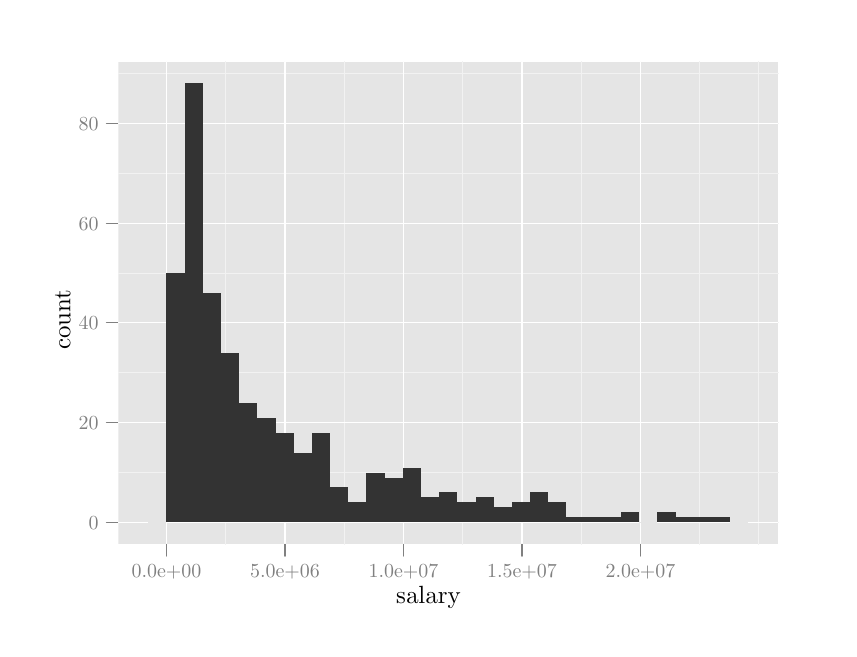
\begin{tikzpicture}[x=1pt,y=1pt]
\draw[color=white,opacity=0] (0,0) rectangle (289.08,216.81);
\begin{scope}
\path[clip] (  0.00,  0.00) rectangle (289.08,216.81);
\definecolor[named]{drawColor}{rgb}{0.66,0.05,0.14}
\end{scope}
\begin{scope}
\path[clip] (  0.00,  0.00) rectangle (289.08,216.81);
\definecolor[named]{drawColor}{rgb}{0.66,0.05,0.14}
\end{scope}
\begin{scope}
\path[clip] (  0.00,  0.00) rectangle (289.08,216.81);
\definecolor[named]{drawColor}{rgb}{0.66,0.05,0.14}
\end{scope}
\begin{scope}
\path[clip] (  0.00,  0.00) rectangle (289.08,216.81);
\definecolor[named]{drawColor}{rgb}{0.66,0.05,0.14}
\end{scope}
\begin{scope}
\path[clip] (  0.00,  0.00) rectangle (289.08,216.81);
\definecolor[named]{drawColor}{rgb}{0.66,0.05,0.14}
\end{scope}
\begin{scope}
\path[clip] (  0.00,  0.00) rectangle (289.08,216.81);
\definecolor[named]{drawColor}{rgb}{0.66,0.05,0.14}
\end{scope}
\begin{scope}
\path[clip] (  0.00,  0.00) rectangle (289.08,216.81);
\definecolor[named]{drawColor}{rgb}{0.66,0.05,0.14}
\end{scope}
\begin{scope}
\path[clip] (  0.00,  0.00) rectangle (289.08,216.81);
\definecolor[named]{drawColor}{rgb}{0.66,0.05,0.14}
\end{scope}
\begin{scope}
\path[clip] (  0.00,  0.00) rectangle (289.08,216.81);
\definecolor[named]{drawColor}{rgb}{0.66,0.05,0.14}
\definecolor[named]{fillColor}{rgb}{1.00,1.00,1.00}

\draw[fill=fillColor,draw opacity=0.00,] (  0.00,  0.00) rectangle (289.08,216.81);
\end{scope}
\begin{scope}
\path[clip] (  0.00,  0.00) rectangle (289.08,216.81);
\definecolor[named]{drawColor}{rgb}{0.66,0.05,0.14}
\end{scope}
\begin{scope}
\path[clip] (  0.00,  0.00) rectangle (289.08,216.81);
\definecolor[named]{drawColor}{rgb}{0.66,0.05,0.14}
\definecolor[named]{drawColor}{rgb}{0.00,0.00,0.00}

\node[color=drawColor,anchor=base,inner sep=0pt, outer sep=0pt, scale=  0.90] at (144.63,  9.03) {salary%
};
\end{scope}
\begin{scope}
\path[clip] (  0.00,  0.00) rectangle (289.08,216.81);
\definecolor[named]{drawColor}{rgb}{0.66,0.05,0.14}
\definecolor[named]{drawColor}{rgb}{0.00,0.00,0.00}

\node[rotate= 90.00,color=drawColor,anchor=base,inner sep=0pt, outer sep=0pt, scale=  0.90] at ( 15.23,111.50) {count%
};
\end{scope}
\begin{scope}
\path[clip] (  0.00,  0.00) rectangle (289.08,216.81);
\definecolor[named]{drawColor}{rgb}{0.66,0.05,0.14}
\end{scope}
\begin{scope}
\path[clip] ( 18.24,204.76) rectangle ( 32.55,204.76);
\definecolor[named]{drawColor}{rgb}{0.66,0.05,0.14}
\end{scope}
\begin{scope}
\path[clip] (  0.00,  0.00) rectangle (289.08,216.81);
\definecolor[named]{drawColor}{rgb}{0.66,0.05,0.14}
\end{scope}
\begin{scope}
\path[clip] ( 18.24,204.76) rectangle ( 32.55,204.76);
\definecolor[named]{drawColor}{rgb}{0.66,0.05,0.14}
\end{scope}
\begin{scope}
\path[clip] (  0.00,  0.00) rectangle (289.08,216.81);
\definecolor[named]{drawColor}{rgb}{0.66,0.05,0.14}
\end{scope}
\begin{scope}
\path[clip] (  0.00,  0.00) rectangle (289.08,216.81);
\definecolor[named]{drawColor}{rgb}{0.66,0.05,0.14}
\end{scope}
\begin{scope}
\path[clip] (  0.00,  0.00) rectangle (289.08,216.81);
\definecolor[named]{drawColor}{rgb}{0.66,0.05,0.14}
\end{scope}
\begin{scope}
\path[clip] ( 18.24, 30.32) rectangle ( 32.55, 30.32);
\definecolor[named]{drawColor}{rgb}{0.66,0.05,0.14}
\end{scope}
\begin{scope}
\path[clip] (  0.00,  0.00) rectangle (289.08,216.81);
\definecolor[named]{drawColor}{rgb}{0.66,0.05,0.14}
\end{scope}
\begin{scope}
\path[clip] ( 18.24, 18.24) rectangle ( 32.55, 30.32);
\definecolor[named]{drawColor}{rgb}{0.66,0.05,0.14}
\end{scope}
\begin{scope}
\path[clip] (  0.00,  0.00) rectangle (289.08,216.81);
\definecolor[named]{drawColor}{rgb}{0.66,0.05,0.14}
\end{scope}
\begin{scope}
\path[clip] ( 18.24, 18.24) rectangle ( 32.55, 18.24);
\definecolor[named]{drawColor}{rgb}{0.66,0.05,0.14}
\end{scope}
\begin{scope}
\path[clip] (  0.00,  0.00) rectangle (289.08,216.81);
\definecolor[named]{drawColor}{rgb}{0.66,0.05,0.14}
\end{scope}
\begin{scope}
\path[clip] ( 32.55,204.76) rectangle ( 32.55,204.76);
\definecolor[named]{drawColor}{rgb}{0.66,0.05,0.14}
\end{scope}
\begin{scope}
\path[clip] (  0.00,  0.00) rectangle (289.08,216.81);
\definecolor[named]{drawColor}{rgb}{0.66,0.05,0.14}
\end{scope}
\begin{scope}
\path[clip] ( 32.55,204.76) rectangle ( 32.55,204.76);
\definecolor[named]{drawColor}{rgb}{0.66,0.05,0.14}
\end{scope}
\begin{scope}
\path[clip] (  0.00,  0.00) rectangle (289.08,216.81);
\definecolor[named]{drawColor}{rgb}{0.66,0.05,0.14}
\end{scope}
\begin{scope}
\path[clip] ( 32.55, 30.32) rectangle ( 32.55,204.77);
\definecolor[named]{drawColor}{rgb}{0.66,0.05,0.14}
\end{scope}
\begin{scope}
\path[clip] (  0.00,  0.00) rectangle (289.08,216.81);
\definecolor[named]{drawColor}{rgb}{0.66,0.05,0.14}
\end{scope}
\begin{scope}
\path[clip] ( 32.55, 30.32) rectangle ( 32.55, 30.32);
\definecolor[named]{drawColor}{rgb}{0.66,0.05,0.14}
\end{scope}
\begin{scope}
\path[clip] (  0.00,  0.00) rectangle (289.08,216.81);
\definecolor[named]{drawColor}{rgb}{0.66,0.05,0.14}
\end{scope}
\begin{scope}
\path[clip] ( 32.55, 18.24) rectangle ( 32.55, 30.32);
\definecolor[named]{drawColor}{rgb}{0.66,0.05,0.14}
\end{scope}
\begin{scope}
\path[clip] (  0.00,  0.00) rectangle (289.08,216.81);
\definecolor[named]{drawColor}{rgb}{0.66,0.05,0.14}
\end{scope}
\begin{scope}
\path[clip] ( 32.55, 18.24) rectangle ( 32.55, 18.24);
\definecolor[named]{drawColor}{rgb}{0.66,0.05,0.14}
\end{scope}
\begin{scope}
\path[clip] (  0.00,  0.00) rectangle (289.08,216.81);
\definecolor[named]{drawColor}{rgb}{0.66,0.05,0.14}
\end{scope}
\begin{scope}
\path[clip] ( 32.55,204.76) rectangle (271.01,204.76);
\definecolor[named]{drawColor}{rgb}{0.66,0.05,0.14}
\end{scope}
\begin{scope}
\path[clip] (  0.00,  0.00) rectangle (289.08,216.81);
\definecolor[named]{drawColor}{rgb}{0.66,0.05,0.14}
\end{scope}
\begin{scope}
\path[clip] ( 32.55,204.76) rectangle (271.01,204.76);
\definecolor[named]{drawColor}{rgb}{0.66,0.05,0.14}
\end{scope}
\begin{scope}
\path[clip] (  0.00,  0.00) rectangle (289.08,216.81);
\definecolor[named]{drawColor}{rgb}{0.66,0.05,0.14}
\end{scope}
\begin{scope}
\path[clip] ( 32.55, 30.32) rectangle (271.01,204.77);
\definecolor[named]{drawColor}{rgb}{0.66,0.05,0.14}
\end{scope}
\begin{scope}
\path[clip] (  0.00,  0.00) rectangle (289.08,216.81);
\definecolor[named]{drawColor}{rgb}{0.66,0.05,0.14}
\end{scope}
\begin{scope}
\path[clip] ( 32.55, 30.32) rectangle (271.01, 30.32);
\definecolor[named]{drawColor}{rgb}{0.66,0.05,0.14}
\end{scope}
\begin{scope}
\path[clip] (  0.00,  0.00) rectangle (289.08,216.81);
\definecolor[named]{drawColor}{rgb}{0.66,0.05,0.14}
\end{scope}
\begin{scope}
\path[clip] (  0.00,  0.00) rectangle (289.08,216.81);
\definecolor[named]{drawColor}{rgb}{0.66,0.05,0.14}
\end{scope}
\begin{scope}
\path[clip] (  0.00,  0.00) rectangle (289.08,216.81);
\definecolor[named]{drawColor}{rgb}{0.66,0.05,0.14}
\end{scope}
\begin{scope}
\path[clip] ( 32.55, 18.24) rectangle (271.01, 18.24);
\definecolor[named]{drawColor}{rgb}{0.66,0.05,0.14}
\end{scope}
\begin{scope}
\path[clip] (  0.00,  0.00) rectangle (289.08,216.81);
\definecolor[named]{drawColor}{rgb}{0.66,0.05,0.14}
\end{scope}
\begin{scope}
\path[clip] (271.01,204.76) rectangle (271.01,204.76);
\definecolor[named]{drawColor}{rgb}{0.66,0.05,0.14}
\end{scope}
\begin{scope}
\path[clip] (  0.00,  0.00) rectangle (289.08,216.81);
\definecolor[named]{drawColor}{rgb}{0.66,0.05,0.14}
\end{scope}
\begin{scope}
\path[clip] (271.01,204.76) rectangle (271.01,204.76);
\definecolor[named]{drawColor}{rgb}{0.66,0.05,0.14}
\end{scope}
\begin{scope}
\path[clip] (  0.00,  0.00) rectangle (289.08,216.81);
\definecolor[named]{drawColor}{rgb}{0.66,0.05,0.14}
\end{scope}
\begin{scope}
\path[clip] (271.01, 30.32) rectangle (271.01,204.77);
\definecolor[named]{drawColor}{rgb}{0.66,0.05,0.14}
\end{scope}
\begin{scope}
\path[clip] (  0.00,  0.00) rectangle (289.08,216.81);
\definecolor[named]{drawColor}{rgb}{0.66,0.05,0.14}
\end{scope}
\begin{scope}
\path[clip] (271.01, 30.32) rectangle (271.01, 30.32);
\definecolor[named]{drawColor}{rgb}{0.66,0.05,0.14}
\end{scope}
\begin{scope}
\path[clip] (  0.00,  0.00) rectangle (289.08,216.81);
\definecolor[named]{drawColor}{rgb}{0.66,0.05,0.14}
\end{scope}
\begin{scope}
\path[clip] (271.01, 18.24) rectangle (271.01, 30.32);
\definecolor[named]{drawColor}{rgb}{0.66,0.05,0.14}
\end{scope}
\begin{scope}
\path[clip] (  0.00,  0.00) rectangle (289.08,216.81);
\definecolor[named]{drawColor}{rgb}{0.66,0.05,0.14}
\end{scope}
\begin{scope}
\path[clip] (271.01, 18.24) rectangle (271.01, 18.24);
\definecolor[named]{drawColor}{rgb}{0.66,0.05,0.14}
\end{scope}
\begin{scope}
\path[clip] (  0.00,  0.00) rectangle (289.08,216.81);
\definecolor[named]{drawColor}{rgb}{0.66,0.05,0.14}
\end{scope}
\begin{scope}
\path[clip] (271.01,204.76) rectangle (271.01,204.76);
\definecolor[named]{drawColor}{rgb}{0.66,0.05,0.14}
\end{scope}
\begin{scope}
\path[clip] (  0.00,  0.00) rectangle (289.08,216.81);
\definecolor[named]{drawColor}{rgb}{0.66,0.05,0.14}
\end{scope}
\begin{scope}
\path[clip] (271.01,204.76) rectangle (271.01,204.76);
\definecolor[named]{drawColor}{rgb}{0.66,0.05,0.14}
\end{scope}
\begin{scope}
\path[clip] (  0.00,  0.00) rectangle (289.08,216.81);
\definecolor[named]{drawColor}{rgb}{0.66,0.05,0.14}
\end{scope}
\begin{scope}
\path[clip] (271.01, 30.32) rectangle (271.01,204.77);
\definecolor[named]{drawColor}{rgb}{0.66,0.05,0.14}
\end{scope}
\begin{scope}
\path[clip] (  0.00,  0.00) rectangle (289.08,216.81);
\definecolor[named]{drawColor}{rgb}{0.66,0.05,0.14}
\end{scope}
\begin{scope}
\path[clip] (271.01, 30.32) rectangle (271.01, 30.32);
\definecolor[named]{drawColor}{rgb}{0.66,0.05,0.14}
\end{scope}
\begin{scope}
\path[clip] (  0.00,  0.00) rectangle (289.08,216.81);
\definecolor[named]{drawColor}{rgb}{0.66,0.05,0.14}
\end{scope}
\begin{scope}
\path[clip] (271.01, 18.24) rectangle (271.01, 30.32);
\definecolor[named]{drawColor}{rgb}{0.66,0.05,0.14}
\end{scope}
\begin{scope}
\path[clip] (  0.00,  0.00) rectangle (289.08,216.81);
\definecolor[named]{drawColor}{rgb}{0.66,0.05,0.14}
\end{scope}
\begin{scope}
\path[clip] (271.01, 18.24) rectangle (271.01, 18.24);
\definecolor[named]{drawColor}{rgb}{0.66,0.05,0.14}
\end{scope}
\begin{scope}
\path[clip] (  0.00,  0.00) rectangle (289.08,216.81);
\definecolor[named]{drawColor}{rgb}{0.66,0.05,0.14}
\end{scope}
\begin{scope}
\path[clip] (271.01,204.76) rectangle (271.01,204.76);
\definecolor[named]{drawColor}{rgb}{0.66,0.05,0.14}
\end{scope}
\begin{scope}
\path[clip] (  0.00,  0.00) rectangle (289.08,216.81);
\definecolor[named]{drawColor}{rgb}{0.66,0.05,0.14}
\end{scope}
\begin{scope}
\path[clip] (271.01,204.76) rectangle (271.01,204.76);
\definecolor[named]{drawColor}{rgb}{0.66,0.05,0.14}
\end{scope}
\begin{scope}
\path[clip] (  0.00,  0.00) rectangle (289.08,216.81);
\definecolor[named]{drawColor}{rgb}{0.66,0.05,0.14}
\end{scope}
\begin{scope}
\path[clip] (271.01, 30.32) rectangle (271.01,204.77);
\definecolor[named]{drawColor}{rgb}{0.66,0.05,0.14}
\end{scope}
\begin{scope}
\path[clip] (  0.00,  0.00) rectangle (289.08,216.81);
\definecolor[named]{drawColor}{rgb}{0.66,0.05,0.14}
\end{scope}
\begin{scope}
\path[clip] (271.01, 30.32) rectangle (271.01, 30.32);
\definecolor[named]{drawColor}{rgb}{0.66,0.05,0.14}
\end{scope}
\begin{scope}
\path[clip] (  0.00,  0.00) rectangle (289.08,216.81);
\definecolor[named]{drawColor}{rgb}{0.66,0.05,0.14}
\end{scope}
\begin{scope}
\path[clip] (271.01, 18.24) rectangle (271.01, 30.32);
\definecolor[named]{drawColor}{rgb}{0.66,0.05,0.14}
\end{scope}
\begin{scope}
\path[clip] (  0.00,  0.00) rectangle (289.08,216.81);
\definecolor[named]{drawColor}{rgb}{0.66,0.05,0.14}
\end{scope}
\begin{scope}
\path[clip] (271.01, 18.24) rectangle (271.01, 18.24);
\definecolor[named]{drawColor}{rgb}{0.66,0.05,0.14}
\end{scope}
\begin{scope}
\path[clip] (  0.00,  0.00) rectangle (289.08,216.81);
\definecolor[named]{drawColor}{rgb}{0.66,0.05,0.14}
\end{scope}
\begin{scope}
\path[clip] ( 18.24,204.76) rectangle ( 32.55,204.76);
\definecolor[named]{drawColor}{rgb}{0.66,0.05,0.14}
\end{scope}
\begin{scope}
\path[clip] (  0.00,  0.00) rectangle (289.08,216.81);
\definecolor[named]{drawColor}{rgb}{0.66,0.05,0.14}
\end{scope}
\begin{scope}
\path[clip] ( 18.24,204.76) rectangle ( 32.55,204.76);
\definecolor[named]{drawColor}{rgb}{0.66,0.05,0.14}
\end{scope}
\begin{scope}
\path[clip] (  0.00,  0.00) rectangle (289.08,216.81);
\definecolor[named]{drawColor}{rgb}{0.66,0.05,0.14}
\end{scope}
\begin{scope}
\path[clip] (  0.00,  0.00) rectangle (289.08,216.81);
\definecolor[named]{drawColor}{rgb}{0.66,0.05,0.14}
\definecolor[named]{drawColor}{rgb}{0.50,0.50,0.50}

\node[color=drawColor,anchor=base east,inner sep=0pt, outer sep=0pt, scale=  0.72] at ( 25.44, 35.77) {0%
};

\node[color=drawColor,anchor=base east,inner sep=0pt, outer sep=0pt, scale=  0.72] at ( 25.44, 71.81) {20%
};

\node[color=drawColor,anchor=base east,inner sep=0pt, outer sep=0pt, scale=  0.72] at ( 25.44,107.85) {40%
};

\node[color=drawColor,anchor=base east,inner sep=0pt, outer sep=0pt, scale=  0.72] at ( 25.44,143.90) {60%
};

\node[color=drawColor,anchor=base east,inner sep=0pt, outer sep=0pt, scale=  0.72] at ( 25.44,179.94) {80%
};
\end{scope}
\begin{scope}
\path[clip] (  0.00,  0.00) rectangle (289.08,216.81);
\definecolor[named]{drawColor}{rgb}{0.66,0.05,0.14}
\definecolor[named]{drawColor}{rgb}{0.50,0.50,0.50}

\draw[color=drawColor,line cap=round,line join=round,fill opacity=0.00,] ( 28.29, 38.24) -- ( 32.55, 38.24);

\draw[color=drawColor,line cap=round,line join=round,fill opacity=0.00,] ( 28.29, 74.29) -- ( 32.55, 74.29);

\draw[color=drawColor,line cap=round,line join=round,fill opacity=0.00,] ( 28.29,110.33) -- ( 32.55,110.33);

\draw[color=drawColor,line cap=round,line join=round,fill opacity=0.00,] ( 28.29,146.37) -- ( 32.55,146.37);

\draw[color=drawColor,line cap=round,line join=round,fill opacity=0.00,] ( 28.29,182.42) -- ( 32.55,182.42);
\end{scope}
\begin{scope}
\path[clip] (  0.00,  0.00) rectangle (289.08,216.81);
\definecolor[named]{drawColor}{rgb}{0.66,0.05,0.14}
\end{scope}
\begin{scope}
\path[clip] (  0.00,  0.00) rectangle (289.08,216.81);
\definecolor[named]{drawColor}{rgb}{0.66,0.05,0.14}
\end{scope}
\begin{scope}
\path[clip] (  0.00,  0.00) rectangle (289.08,216.81);
\definecolor[named]{drawColor}{rgb}{0.66,0.05,0.14}
\end{scope}
\begin{scope}
\path[clip] ( 18.24, 30.32) rectangle ( 32.55, 30.32);
\definecolor[named]{drawColor}{rgb}{0.66,0.05,0.14}
\end{scope}
\begin{scope}
\path[clip] (  0.00,  0.00) rectangle (289.08,216.81);
\definecolor[named]{drawColor}{rgb}{0.66,0.05,0.14}
\end{scope}
\begin{scope}
\path[clip] ( 18.24, 18.24) rectangle ( 32.55, 30.32);
\definecolor[named]{drawColor}{rgb}{0.66,0.05,0.14}
\end{scope}
\begin{scope}
\path[clip] (  0.00,  0.00) rectangle (289.08,216.81);
\definecolor[named]{drawColor}{rgb}{0.66,0.05,0.14}
\end{scope}
\begin{scope}
\path[clip] ( 18.24, 18.24) rectangle ( 32.55, 18.24);
\definecolor[named]{drawColor}{rgb}{0.66,0.05,0.14}
\end{scope}
\begin{scope}
\path[clip] (  0.00,  0.00) rectangle (289.08,216.81);
\definecolor[named]{drawColor}{rgb}{0.66,0.05,0.14}
\end{scope}
\begin{scope}
\path[clip] ( 32.55,204.76) rectangle ( 32.55,204.76);
\definecolor[named]{drawColor}{rgb}{0.66,0.05,0.14}
\end{scope}
\begin{scope}
\path[clip] (  0.00,  0.00) rectangle (289.08,216.81);
\definecolor[named]{drawColor}{rgb}{0.66,0.05,0.14}
\end{scope}
\begin{scope}
\path[clip] ( 32.55,204.76) rectangle ( 32.55,204.76);
\definecolor[named]{drawColor}{rgb}{0.66,0.05,0.14}
\end{scope}
\begin{scope}
\path[clip] (  0.00,  0.00) rectangle (289.08,216.81);
\definecolor[named]{drawColor}{rgb}{0.66,0.05,0.14}
\end{scope}
\begin{scope}
\path[clip] ( 32.55, 30.32) rectangle ( 32.55,204.77);
\definecolor[named]{drawColor}{rgb}{0.66,0.05,0.14}
\end{scope}
\begin{scope}
\path[clip] (  0.00,  0.00) rectangle (289.08,216.81);
\definecolor[named]{drawColor}{rgb}{0.66,0.05,0.14}
\end{scope}
\begin{scope}
\path[clip] ( 32.55, 30.32) rectangle ( 32.55, 30.32);
\definecolor[named]{drawColor}{rgb}{0.66,0.05,0.14}
\end{scope}
\begin{scope}
\path[clip] (  0.00,  0.00) rectangle (289.08,216.81);
\definecolor[named]{drawColor}{rgb}{0.66,0.05,0.14}
\end{scope}
\begin{scope}
\path[clip] ( 32.55, 18.24) rectangle ( 32.55, 30.32);
\definecolor[named]{drawColor}{rgb}{0.66,0.05,0.14}
\end{scope}
\begin{scope}
\path[clip] (  0.00,  0.00) rectangle (289.08,216.81);
\definecolor[named]{drawColor}{rgb}{0.66,0.05,0.14}
\end{scope}
\begin{scope}
\path[clip] ( 32.55, 18.24) rectangle ( 32.55, 18.24);
\definecolor[named]{drawColor}{rgb}{0.66,0.05,0.14}
\end{scope}
\begin{scope}
\path[clip] (  0.00,  0.00) rectangle (289.08,216.81);
\definecolor[named]{drawColor}{rgb}{0.66,0.05,0.14}
\end{scope}
\begin{scope}
\path[clip] ( 32.55,204.76) rectangle (271.01,204.76);
\definecolor[named]{drawColor}{rgb}{0.66,0.05,0.14}
\end{scope}
\begin{scope}
\path[clip] (  0.00,  0.00) rectangle (289.08,216.81);
\definecolor[named]{drawColor}{rgb}{0.66,0.05,0.14}
\end{scope}
\begin{scope}
\path[clip] ( 32.55,204.76) rectangle (271.01,204.76);
\definecolor[named]{drawColor}{rgb}{0.66,0.05,0.14}
\end{scope}
\begin{scope}
\path[clip] (  0.00,  0.00) rectangle (289.08,216.81);
\definecolor[named]{drawColor}{rgb}{0.66,0.05,0.14}
\end{scope}
\begin{scope}
\path[clip] ( 32.55, 30.32) rectangle (271.01,204.77);
\definecolor[named]{drawColor}{rgb}{0.66,0.05,0.14}
\definecolor[named]{fillColor}{rgb}{0.90,0.90,0.90}

\draw[fill=fillColor,draw opacity=0.00,] ( 32.55, 30.32) rectangle (271.01,204.77);
\definecolor[named]{drawColor}{rgb}{0.95,0.95,0.95}

\draw[color=drawColor,line width= 0.0pt,line cap=round,line join=round,fill opacity=0.00,] ( 32.55, 38.24) --
	(271.01, 38.24);

\draw[color=drawColor,line width= 0.0pt,line cap=round,line join=round,fill opacity=0.00,] ( 32.55, 56.27) --
	(271.01, 56.27);

\draw[color=drawColor,line width= 0.0pt,line cap=round,line join=round,fill opacity=0.00,] ( 32.55, 74.29) --
	(271.01, 74.29);

\draw[color=drawColor,line width= 0.0pt,line cap=round,line join=round,fill opacity=0.00,] ( 32.55, 92.31) --
	(271.01, 92.31);

\draw[color=drawColor,line width= 0.0pt,line cap=round,line join=round,fill opacity=0.00,] ( 32.55,110.33) --
	(271.01,110.33);

\draw[color=drawColor,line width= 0.0pt,line cap=round,line join=round,fill opacity=0.00,] ( 32.55,128.35) --
	(271.01,128.35);

\draw[color=drawColor,line width= 0.0pt,line cap=round,line join=round,fill opacity=0.00,] ( 32.55,146.37) --
	(271.01,146.37);

\draw[color=drawColor,line width= 0.0pt,line cap=round,line join=round,fill opacity=0.00,] ( 32.55,164.40) --
	(271.01,164.40);

\draw[color=drawColor,line width= 0.0pt,line cap=round,line join=round,fill opacity=0.00,] ( 32.55,182.42) --
	(271.01,182.42);

\draw[color=drawColor,line width= 0.0pt,line cap=round,line join=round,fill opacity=0.00,] ( 32.55,200.44) --
	(271.01,200.44);

\draw[color=drawColor,line width= 0.0pt,line cap=round,line join=round,fill opacity=0.00,] ( 49.96, 30.32) --
	( 49.96,204.77);

\draw[color=drawColor,line width= 0.0pt,line cap=round,line join=round,fill opacity=0.00,] ( 71.37, 30.32) --
	( 71.37,204.77);

\draw[color=drawColor,line width= 0.0pt,line cap=round,line join=round,fill opacity=0.00,] ( 92.78, 30.32) --
	( 92.78,204.77);

\draw[color=drawColor,line width= 0.0pt,line cap=round,line join=round,fill opacity=0.00,] (114.19, 30.32) --
	(114.19,204.77);

\draw[color=drawColor,line width= 0.0pt,line cap=round,line join=round,fill opacity=0.00,] (135.60, 30.32) --
	(135.60,204.77);

\draw[color=drawColor,line width= 0.0pt,line cap=round,line join=round,fill opacity=0.00,] (157.01, 30.32) --
	(157.01,204.77);

\draw[color=drawColor,line width= 0.0pt,line cap=round,line join=round,fill opacity=0.00,] (178.41, 30.32) --
	(178.41,204.77);

\draw[color=drawColor,line width= 0.0pt,line cap=round,line join=round,fill opacity=0.00,] (199.82, 30.32) --
	(199.82,204.77);

\draw[color=drawColor,line width= 0.0pt,line cap=round,line join=round,fill opacity=0.00,] (221.23, 30.32) --
	(221.23,204.77);

\draw[color=drawColor,line width= 0.0pt,line cap=round,line join=round,fill opacity=0.00,] (242.64, 30.32) --
	(242.64,204.77);

\draw[color=drawColor,line width= 0.0pt,line cap=round,line join=round,fill opacity=0.00,] (264.05, 30.32) --
	(264.05,204.77);
\definecolor[named]{drawColor}{rgb}{1.00,1.00,1.00}

\draw[color=drawColor,line cap=round,line join=round,fill opacity=0.00,] ( 32.55, 38.24) --
	(271.01, 38.24);

\draw[color=drawColor,line cap=round,line join=round,fill opacity=0.00,] ( 32.55, 74.29) --
	(271.01, 74.29);

\draw[color=drawColor,line cap=round,line join=round,fill opacity=0.00,] ( 32.55,110.33) --
	(271.01,110.33);

\draw[color=drawColor,line cap=round,line join=round,fill opacity=0.00,] ( 32.55,146.37) --
	(271.01,146.37);

\draw[color=drawColor,line cap=round,line join=round,fill opacity=0.00,] ( 32.55,182.42) --
	(271.01,182.42);

\draw[color=drawColor,line cap=round,line join=round,fill opacity=0.00,] ( 49.96, 30.32) --
	( 49.96,204.77);

\draw[color=drawColor,line cap=round,line join=round,fill opacity=0.00,] ( 92.78, 30.32) --
	( 92.78,204.77);

\draw[color=drawColor,line cap=round,line join=round,fill opacity=0.00,] (135.60, 30.32) --
	(135.60,204.77);

\draw[color=drawColor,line cap=round,line join=round,fill opacity=0.00,] (178.41, 30.32) --
	(178.41,204.77);

\draw[color=drawColor,line cap=round,line join=round,fill opacity=0.00,] (221.23, 30.32) --
	(221.23,204.77);
\definecolor[named]{fillColor}{rgb}{0.20,0.20,0.20}

\draw[fill=fillColor,draw opacity=0.00,] ( 43.39, 38.24) rectangle ( 49.96, 38.24);

\draw[fill=fillColor,draw opacity=0.00,] ( 49.96, 38.24) rectangle ( 56.53,128.35);

\draw[fill=fillColor,draw opacity=0.00,] ( 56.53, 38.24) rectangle ( 63.10,196.84);

\draw[fill=fillColor,draw opacity=0.00,] ( 63.10, 38.24) rectangle ( 69.67,121.14);

\draw[fill=fillColor,draw opacity=0.00,] ( 69.67, 38.24) rectangle ( 76.24, 99.52);

\draw[fill=fillColor,draw opacity=0.00,] ( 76.24, 38.24) rectangle ( 82.81, 81.50);

\draw[fill=fillColor,draw opacity=0.00,] ( 82.81, 38.24) rectangle ( 89.38, 76.09);

\draw[fill=fillColor,draw opacity=0.00,] ( 89.38, 38.24) rectangle ( 95.95, 70.68);

\draw[fill=fillColor,draw opacity=0.00,] ( 95.95, 38.24) rectangle (102.52, 63.48);

\draw[fill=fillColor,draw opacity=0.00,] (102.52, 38.24) rectangle (109.08, 70.68);

\draw[fill=fillColor,draw opacity=0.00,] (109.08, 38.24) rectangle (115.65, 50.86);

\draw[fill=fillColor,draw opacity=0.00,] (115.65, 38.24) rectangle (122.22, 45.45);

\draw[fill=fillColor,draw opacity=0.00,] (122.22, 38.24) rectangle (128.79, 56.27);

\draw[fill=fillColor,draw opacity=0.00,] (128.79, 38.24) rectangle (135.36, 54.46);

\draw[fill=fillColor,draw opacity=0.00,] (135.36, 38.24) rectangle (141.93, 58.07);

\draw[fill=fillColor,draw opacity=0.00,] (141.93, 38.24) rectangle (148.50, 47.26);

\draw[fill=fillColor,draw opacity=0.00,] (148.50, 38.24) rectangle (155.07, 49.06);

\draw[fill=fillColor,draw opacity=0.00,] (155.07, 38.24) rectangle (161.64, 45.45);

\draw[fill=fillColor,draw opacity=0.00,] (161.64, 38.24) rectangle (168.21, 47.26);

\draw[fill=fillColor,draw opacity=0.00,] (168.21, 38.24) rectangle (174.78, 43.65);

\draw[fill=fillColor,draw opacity=0.00,] (174.78, 38.24) rectangle (181.34, 45.45);

\draw[fill=fillColor,draw opacity=0.00,] (181.34, 38.24) rectangle (187.91, 49.06);

\draw[fill=fillColor,draw opacity=0.00,] (187.91, 38.24) rectangle (194.48, 45.45);

\draw[fill=fillColor,draw opacity=0.00,] (194.48, 38.24) rectangle (201.05, 40.05);

\draw[fill=fillColor,draw opacity=0.00,] (201.05, 38.24) rectangle (207.62, 40.05);

\draw[fill=fillColor,draw opacity=0.00,] (207.62, 38.24) rectangle (214.19, 40.05);

\draw[fill=fillColor,draw opacity=0.00,] (214.19, 38.24) rectangle (220.76, 41.85);

\draw[fill=fillColor,draw opacity=0.00,] (220.76, 38.24) rectangle (227.33, 38.24);

\draw[fill=fillColor,draw opacity=0.00,] (227.33, 38.24) rectangle (233.90, 41.85);

\draw[fill=fillColor,draw opacity=0.00,] (233.90, 38.24) rectangle (240.47, 40.05);

\draw[fill=fillColor,draw opacity=0.00,] (240.47, 38.24) rectangle (247.04, 40.05);

\draw[fill=fillColor,draw opacity=0.00,] (247.04, 38.24) rectangle (253.60, 40.05);

\draw[fill=fillColor,draw opacity=0.00,] (253.60, 38.24) rectangle (260.17, 38.24);
\end{scope}
\begin{scope}
\path[clip] (  0.00,  0.00) rectangle (289.08,216.81);
\definecolor[named]{drawColor}{rgb}{0.66,0.05,0.14}
\end{scope}
\begin{scope}
\path[clip] ( 32.55, 30.32) rectangle (271.01, 30.32);
\definecolor[named]{drawColor}{rgb}{0.66,0.05,0.14}
\end{scope}
\begin{scope}
\path[clip] (  0.00,  0.00) rectangle (289.08,216.81);
\definecolor[named]{drawColor}{rgb}{0.66,0.05,0.14}
\end{scope}
\begin{scope}
\path[clip] (  0.00,  0.00) rectangle (289.08,216.81);
\definecolor[named]{drawColor}{rgb}{0.66,0.05,0.14}
\definecolor[named]{drawColor}{rgb}{0.50,0.50,0.50}

\node[color=drawColor,anchor=base,inner sep=0pt, outer sep=0pt, scale=  0.72] at ( 49.96, 18.24) {0.0e+00%
};

\node[color=drawColor,anchor=base,inner sep=0pt, outer sep=0pt, scale=  0.72] at ( 92.78, 18.24) {5.0e+06%
};

\node[color=drawColor,anchor=base,inner sep=0pt, outer sep=0pt, scale=  0.72] at (135.60, 18.24) {1.0e+07%
};

\node[color=drawColor,anchor=base,inner sep=0pt, outer sep=0pt, scale=  0.72] at (178.41, 18.24) {1.5e+07%
};

\node[color=drawColor,anchor=base,inner sep=0pt, outer sep=0pt, scale=  0.72] at (221.23, 18.24) {2.0e+07%
};
\end{scope}
\begin{scope}
\path[clip] (  0.00,  0.00) rectangle (289.08,216.81);
\definecolor[named]{drawColor}{rgb}{0.66,0.05,0.14}
\definecolor[named]{drawColor}{rgb}{0.50,0.50,0.50}

\draw[color=drawColor,line cap=round,line join=round,fill opacity=0.00,] ( 49.96, 26.05) -- ( 49.96, 30.32);

\draw[color=drawColor,line cap=round,line join=round,fill opacity=0.00,] ( 92.78, 26.05) -- ( 92.78, 30.32);

\draw[color=drawColor,line cap=round,line join=round,fill opacity=0.00,] (135.60, 26.05) -- (135.60, 30.32);

\draw[color=drawColor,line cap=round,line join=round,fill opacity=0.00,] (178.41, 26.05) -- (178.41, 30.32);

\draw[color=drawColor,line cap=round,line join=round,fill opacity=0.00,] (221.23, 26.05) -- (221.23, 30.32);
\end{scope}
\begin{scope}
\path[clip] (  0.00,  0.00) rectangle (289.08,216.81);
\definecolor[named]{drawColor}{rgb}{0.66,0.05,0.14}
\end{scope}
\begin{scope}
\path[clip] (  0.00,  0.00) rectangle (289.08,216.81);
\definecolor[named]{drawColor}{rgb}{0.66,0.05,0.14}
\end{scope}
\begin{scope}
\path[clip] (  0.00,  0.00) rectangle (289.08,216.81);
\definecolor[named]{drawColor}{rgb}{0.66,0.05,0.14}
\end{scope}
\begin{scope}
\path[clip] ( 32.55, 18.24) rectangle (271.01, 18.24);
\definecolor[named]{drawColor}{rgb}{0.66,0.05,0.14}
\end{scope}
\begin{scope}
\path[clip] (  0.00,  0.00) rectangle (289.08,216.81);
\definecolor[named]{drawColor}{rgb}{0.66,0.05,0.14}
\end{scope}
\begin{scope}
\path[clip] (271.01,204.76) rectangle (271.01,204.76);
\definecolor[named]{drawColor}{rgb}{0.66,0.05,0.14}
\end{scope}
\begin{scope}
\path[clip] (  0.00,  0.00) rectangle (289.08,216.81);
\definecolor[named]{drawColor}{rgb}{0.66,0.05,0.14}
\end{scope}
\begin{scope}
\path[clip] (271.01,204.76) rectangle (271.01,204.76);
\definecolor[named]{drawColor}{rgb}{0.66,0.05,0.14}
\end{scope}
\begin{scope}
\path[clip] (  0.00,  0.00) rectangle (289.08,216.81);
\definecolor[named]{drawColor}{rgb}{0.66,0.05,0.14}
\end{scope}
\begin{scope}
\path[clip] (271.01, 30.32) rectangle (271.01,204.77);
\definecolor[named]{drawColor}{rgb}{0.66,0.05,0.14}
\end{scope}
\begin{scope}
\path[clip] (  0.00,  0.00) rectangle (289.08,216.81);
\definecolor[named]{drawColor}{rgb}{0.66,0.05,0.14}
\end{scope}
\begin{scope}
\path[clip] (271.01, 30.32) rectangle (271.01, 30.32);
\definecolor[named]{drawColor}{rgb}{0.66,0.05,0.14}
\end{scope}
\begin{scope}
\path[clip] (  0.00,  0.00) rectangle (289.08,216.81);
\definecolor[named]{drawColor}{rgb}{0.66,0.05,0.14}
\end{scope}
\begin{scope}
\path[clip] (271.01, 18.24) rectangle (271.01, 30.32);
\definecolor[named]{drawColor}{rgb}{0.66,0.05,0.14}
\end{scope}
\begin{scope}
\path[clip] (  0.00,  0.00) rectangle (289.08,216.81);
\definecolor[named]{drawColor}{rgb}{0.66,0.05,0.14}
\end{scope}
\begin{scope}
\path[clip] (271.01, 18.24) rectangle (271.01, 18.24);
\definecolor[named]{drawColor}{rgb}{0.66,0.05,0.14}
\end{scope}
\begin{scope}
\path[clip] (  0.00,  0.00) rectangle (289.08,216.81);
\definecolor[named]{drawColor}{rgb}{0.66,0.05,0.14}
\end{scope}
\begin{scope}
\path[clip] (271.01,204.76) rectangle (271.01,204.76);
\definecolor[named]{drawColor}{rgb}{0.66,0.05,0.14}
\end{scope}
\begin{scope}
\path[clip] (  0.00,  0.00) rectangle (289.08,216.81);
\definecolor[named]{drawColor}{rgb}{0.66,0.05,0.14}
\end{scope}
\begin{scope}
\path[clip] (271.01,204.76) rectangle (271.01,204.76);
\definecolor[named]{drawColor}{rgb}{0.66,0.05,0.14}
\end{scope}
\begin{scope}
\path[clip] (  0.00,  0.00) rectangle (289.08,216.81);
\definecolor[named]{drawColor}{rgb}{0.66,0.05,0.14}
\end{scope}
\begin{scope}
\path[clip] (271.01, 30.32) rectangle (271.01,204.77);
\definecolor[named]{drawColor}{rgb}{0.66,0.05,0.14}
\end{scope}
\begin{scope}
\path[clip] (  0.00,  0.00) rectangle (289.08,216.81);
\definecolor[named]{drawColor}{rgb}{0.66,0.05,0.14}
\end{scope}
\begin{scope}
\path[clip] (271.01, 30.32) rectangle (271.01, 30.32);
\definecolor[named]{drawColor}{rgb}{0.66,0.05,0.14}
\end{scope}
\begin{scope}
\path[clip] (  0.00,  0.00) rectangle (289.08,216.81);
\definecolor[named]{drawColor}{rgb}{0.66,0.05,0.14}
\end{scope}
\begin{scope}
\path[clip] (271.01, 18.24) rectangle (271.01, 30.32);
\definecolor[named]{drawColor}{rgb}{0.66,0.05,0.14}
\end{scope}
\begin{scope}
\path[clip] (  0.00,  0.00) rectangle (289.08,216.81);
\definecolor[named]{drawColor}{rgb}{0.66,0.05,0.14}
\end{scope}
\begin{scope}
\path[clip] (271.01, 18.24) rectangle (271.01, 18.24);
\definecolor[named]{drawColor}{rgb}{0.66,0.05,0.14}
\end{scope}
\begin{scope}
\path[clip] (  0.00,  0.00) rectangle (289.08,216.81);
\definecolor[named]{drawColor}{rgb}{0.66,0.05,0.14}
\end{scope}
\begin{scope}
\path[clip] (271.01,204.76) rectangle (271.01,204.76);
\definecolor[named]{drawColor}{rgb}{0.66,0.05,0.14}
\end{scope}
\begin{scope}
\path[clip] (  0.00,  0.00) rectangle (289.08,216.81);
\definecolor[named]{drawColor}{rgb}{0.66,0.05,0.14}
\end{scope}
\begin{scope}
\path[clip] (271.01,204.76) rectangle (271.01,204.76);
\definecolor[named]{drawColor}{rgb}{0.66,0.05,0.14}
\end{scope}
\begin{scope}
\path[clip] (  0.00,  0.00) rectangle (289.08,216.81);
\definecolor[named]{drawColor}{rgb}{0.66,0.05,0.14}
\end{scope}
\begin{scope}
\path[clip] (271.01, 30.32) rectangle (271.01,204.77);
\definecolor[named]{drawColor}{rgb}{0.66,0.05,0.14}
\end{scope}
\begin{scope}
\path[clip] (  0.00,  0.00) rectangle (289.08,216.81);
\definecolor[named]{drawColor}{rgb}{0.66,0.05,0.14}
\end{scope}
\begin{scope}
\path[clip] (271.01, 30.32) rectangle (271.01, 30.32);
\definecolor[named]{drawColor}{rgb}{0.66,0.05,0.14}
\end{scope}
\begin{scope}
\path[clip] (  0.00,  0.00) rectangle (289.08,216.81);
\definecolor[named]{drawColor}{rgb}{0.66,0.05,0.14}
\end{scope}
\begin{scope}
\path[clip] (271.01, 18.24) rectangle (271.01, 30.32);
\definecolor[named]{drawColor}{rgb}{0.66,0.05,0.14}
\end{scope}
\begin{scope}
\path[clip] (  0.00,  0.00) rectangle (289.08,216.81);
\definecolor[named]{drawColor}{rgb}{0.66,0.05,0.14}
\end{scope}
\begin{scope}
\path[clip] (271.01, 18.24) rectangle (271.01, 18.24);
\definecolor[named]{drawColor}{rgb}{0.66,0.05,0.14}
\end{scope}
\begin{scope}
\path[clip] (  0.00,  0.00) rectangle (289.08,216.81);
\definecolor[named]{drawColor}{rgb}{0.66,0.05,0.14}
\end{scope}
\begin{scope}
\path[clip] (  0.00,  0.00) rectangle (289.08,216.81);
\definecolor[named]{drawColor}{rgb}{0.66,0.05,0.14}
\end{scope}
\begin{scope}
\path[clip] (  0.00,  0.00) rectangle (289.08,216.81);
\definecolor[named]{drawColor}{rgb}{0.66,0.05,0.14}
\end{scope}
\end{tikzpicture}

\endpgfgraphicnamed
\end{center}
\end{dummy}
\caption{The distribution of salary: the histogram is severely skewed to the
right. The range of salaries is very large, and often there are only
a few key players to a team.\label{fig:hist-salary}}

\end{figure}


In this section we will give a summary of the dataset. Since our direct
goal is to predict salary, it is natural to take a look at the distribution
of the salary in Figure \ref{fig:hist-salary}, which is skewed to
the right and has a long tail. This may indicate a log-transformation
of the salary data, and we will see later the effects of transformation.

%
\begin{figure}
\begin{dummy}
\hspace*{\fill}\\
\hlstd{}\ttfamily\noindent
\hlprompt{\usebox{\hlnormalsizeboxgreaterthan}{\ }}\hlfunctioncall{print}\hlkeyword{(}\hlfunctioncall{qplot}\hlkeyword{(}\hlsymbol{minutes}\hlkeyword{,}{\ }\hlsymbol{salary}\hlkeyword{,}{\ }\hlargument{data}{\ }\hlargument{=}{\ }\hlsymbol{bb}\hlkeyword{,}{\ }\hlargument{geom}{\ }\hlargument{=}{\ }\hlfunctioncall{c}\hlkeyword{(}\hlstring{"point"}\hlkeyword{,}{\ }\hlstring{"smooth"}\hlkeyword{)}\hlkeyword{)}\hlkeyword{)}\mbox{}
\normalfont
\hspace*{\fill}\\
\hlstd{}
\begin{center}

\beginpgfgraphicnamed{figure/Rfig-salary-minutes}
% Created by tikzDevice version 0.5.3 on 2011-01-28 19:54:27
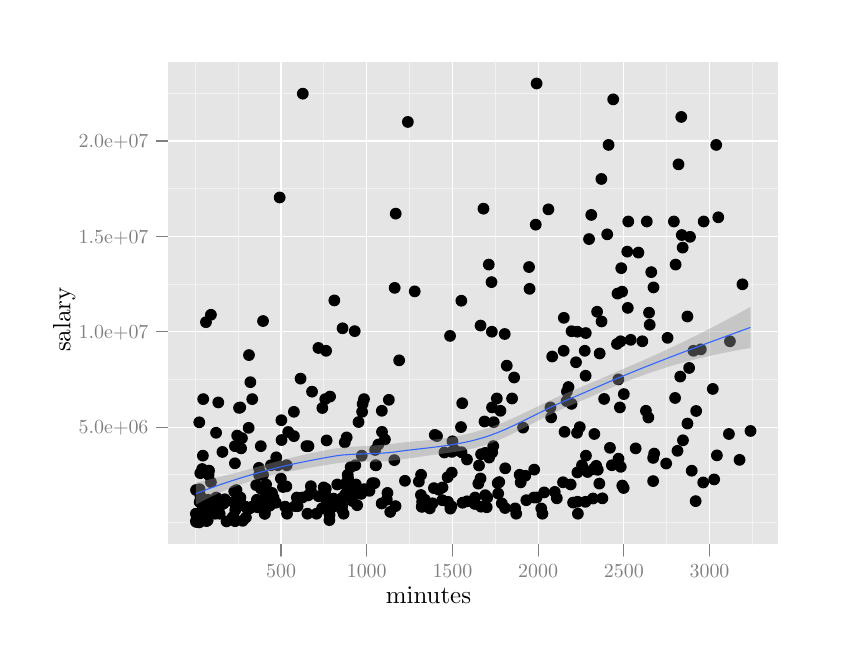
\begin{tikzpicture}[x=1pt,y=1pt]
\draw[color=white,opacity=0] (0,0) rectangle (289.08,216.81);
\begin{scope}
\path[clip] (  0.00,  0.00) rectangle (289.08,216.81);
\definecolor[named]{drawColor}{rgb}{0.44,0.35,0.31}
\end{scope}
\begin{scope}
\path[clip] (  0.00,  0.00) rectangle (289.08,216.81);
\definecolor[named]{drawColor}{rgb}{0.44,0.35,0.31}
\end{scope}
\begin{scope}
\path[clip] (  0.00,  0.00) rectangle (289.08,216.81);
\definecolor[named]{drawColor}{rgb}{0.44,0.35,0.31}
\end{scope}
\begin{scope}
\path[clip] (  0.00,  0.00) rectangle (289.08,216.81);
\definecolor[named]{drawColor}{rgb}{0.44,0.35,0.31}
\end{scope}
\begin{scope}
\path[clip] (  0.00,  0.00) rectangle (289.08,216.81);
\definecolor[named]{drawColor}{rgb}{0.44,0.35,0.31}
\end{scope}
\begin{scope}
\path[clip] (  0.00,  0.00) rectangle (289.08,216.81);
\definecolor[named]{drawColor}{rgb}{0.44,0.35,0.31}
\end{scope}
\begin{scope}
\path[clip] (  0.00,  0.00) rectangle (289.08,216.81);
\definecolor[named]{drawColor}{rgb}{0.44,0.35,0.31}
\end{scope}
\begin{scope}
\path[clip] (  0.00,  0.00) rectangle (289.08,216.81);
\definecolor[named]{drawColor}{rgb}{0.44,0.35,0.31}
\end{scope}
\begin{scope}
\path[clip] (  0.00,  0.00) rectangle (289.08,216.81);
\definecolor[named]{drawColor}{rgb}{0.44,0.35,0.31}
\definecolor[named]{fillColor}{rgb}{1.00,1.00,1.00}

\draw[fill=fillColor,draw opacity=0.00,] (  0.00,  0.00) rectangle (289.08,216.81);
\end{scope}
\begin{scope}
\path[clip] (  0.00,  0.00) rectangle (289.08,216.81);
\definecolor[named]{drawColor}{rgb}{0.44,0.35,0.31}
\end{scope}
\begin{scope}
\path[clip] (  0.00,  0.00) rectangle (289.08,216.81);
\definecolor[named]{drawColor}{rgb}{0.44,0.35,0.31}
\definecolor[named]{drawColor}{rgb}{0.00,0.00,0.00}

\node[color=drawColor,anchor=base,inner sep=0pt, outer sep=0pt, scale=  0.90] at (144.63,  9.03) {minutes%
};
\end{scope}
\begin{scope}
\path[clip] (  0.00,  0.00) rectangle (289.08,216.81);
\definecolor[named]{drawColor}{rgb}{0.44,0.35,0.31}
\definecolor[named]{drawColor}{rgb}{0.00,0.00,0.00}

\node[rotate= 90.00,color=drawColor,anchor=base,inner sep=0pt, outer sep=0pt, scale=  0.90] at ( 15.23,111.50) {salary%
};
\end{scope}
\begin{scope}
\path[clip] (  0.00,  0.00) rectangle (289.08,216.81);
\definecolor[named]{drawColor}{rgb}{0.44,0.35,0.31}
\end{scope}
\begin{scope}
\path[clip] ( 18.24,204.76) rectangle ( 50.55,204.76);
\definecolor[named]{drawColor}{rgb}{0.44,0.35,0.31}
\end{scope}
\begin{scope}
\path[clip] (  0.00,  0.00) rectangle (289.08,216.81);
\definecolor[named]{drawColor}{rgb}{0.44,0.35,0.31}
\end{scope}
\begin{scope}
\path[clip] ( 18.24,204.76) rectangle ( 50.55,204.76);
\definecolor[named]{drawColor}{rgb}{0.44,0.35,0.31}
\end{scope}
\begin{scope}
\path[clip] (  0.00,  0.00) rectangle (289.08,216.81);
\definecolor[named]{drawColor}{rgb}{0.44,0.35,0.31}
\end{scope}
\begin{scope}
\path[clip] (  0.00,  0.00) rectangle (289.08,216.81);
\definecolor[named]{drawColor}{rgb}{0.44,0.35,0.31}
\end{scope}
\begin{scope}
\path[clip] (  0.00,  0.00) rectangle (289.08,216.81);
\definecolor[named]{drawColor}{rgb}{0.44,0.35,0.31}
\end{scope}
\begin{scope}
\path[clip] ( 18.24, 30.32) rectangle ( 50.55, 30.32);
\definecolor[named]{drawColor}{rgb}{0.44,0.35,0.31}
\end{scope}
\begin{scope}
\path[clip] (  0.00,  0.00) rectangle (289.08,216.81);
\definecolor[named]{drawColor}{rgb}{0.44,0.35,0.31}
\end{scope}
\begin{scope}
\path[clip] ( 18.24, 18.24) rectangle ( 50.55, 30.32);
\definecolor[named]{drawColor}{rgb}{0.44,0.35,0.31}
\end{scope}
\begin{scope}
\path[clip] (  0.00,  0.00) rectangle (289.08,216.81);
\definecolor[named]{drawColor}{rgb}{0.44,0.35,0.31}
\end{scope}
\begin{scope}
\path[clip] ( 18.24, 18.24) rectangle ( 50.55, 18.24);
\definecolor[named]{drawColor}{rgb}{0.44,0.35,0.31}
\end{scope}
\begin{scope}
\path[clip] (  0.00,  0.00) rectangle (289.08,216.81);
\definecolor[named]{drawColor}{rgb}{0.44,0.35,0.31}
\end{scope}
\begin{scope}
\path[clip] ( 50.55,204.76) rectangle ( 50.55,204.76);
\definecolor[named]{drawColor}{rgb}{0.44,0.35,0.31}
\end{scope}
\begin{scope}
\path[clip] (  0.00,  0.00) rectangle (289.08,216.81);
\definecolor[named]{drawColor}{rgb}{0.44,0.35,0.31}
\end{scope}
\begin{scope}
\path[clip] ( 50.55,204.76) rectangle ( 50.55,204.76);
\definecolor[named]{drawColor}{rgb}{0.44,0.35,0.31}
\end{scope}
\begin{scope}
\path[clip] (  0.00,  0.00) rectangle (289.08,216.81);
\definecolor[named]{drawColor}{rgb}{0.44,0.35,0.31}
\end{scope}
\begin{scope}
\path[clip] ( 50.55, 30.32) rectangle ( 50.55,204.77);
\definecolor[named]{drawColor}{rgb}{0.44,0.35,0.31}
\end{scope}
\begin{scope}
\path[clip] (  0.00,  0.00) rectangle (289.08,216.81);
\definecolor[named]{drawColor}{rgb}{0.44,0.35,0.31}
\end{scope}
\begin{scope}
\path[clip] ( 50.55, 30.32) rectangle ( 50.55, 30.32);
\definecolor[named]{drawColor}{rgb}{0.44,0.35,0.31}
\end{scope}
\begin{scope}
\path[clip] (  0.00,  0.00) rectangle (289.08,216.81);
\definecolor[named]{drawColor}{rgb}{0.44,0.35,0.31}
\end{scope}
\begin{scope}
\path[clip] ( 50.55, 18.24) rectangle ( 50.55, 30.32);
\definecolor[named]{drawColor}{rgb}{0.44,0.35,0.31}
\end{scope}
\begin{scope}
\path[clip] (  0.00,  0.00) rectangle (289.08,216.81);
\definecolor[named]{drawColor}{rgb}{0.44,0.35,0.31}
\end{scope}
\begin{scope}
\path[clip] ( 50.55, 18.24) rectangle ( 50.55, 18.24);
\definecolor[named]{drawColor}{rgb}{0.44,0.35,0.31}
\end{scope}
\begin{scope}
\path[clip] (  0.00,  0.00) rectangle (289.08,216.81);
\definecolor[named]{drawColor}{rgb}{0.44,0.35,0.31}
\end{scope}
\begin{scope}
\path[clip] ( 50.55,204.76) rectangle (271.01,204.76);
\definecolor[named]{drawColor}{rgb}{0.44,0.35,0.31}
\end{scope}
\begin{scope}
\path[clip] (  0.00,  0.00) rectangle (289.08,216.81);
\definecolor[named]{drawColor}{rgb}{0.44,0.35,0.31}
\end{scope}
\begin{scope}
\path[clip] ( 50.55,204.76) rectangle (271.01,204.76);
\definecolor[named]{drawColor}{rgb}{0.44,0.35,0.31}
\end{scope}
\begin{scope}
\path[clip] (  0.00,  0.00) rectangle (289.08,216.81);
\definecolor[named]{drawColor}{rgb}{0.44,0.35,0.31}
\end{scope}
\begin{scope}
\path[clip] ( 50.55, 30.32) rectangle (271.01,204.77);
\definecolor[named]{drawColor}{rgb}{0.44,0.35,0.31}
\end{scope}
\begin{scope}
\path[clip] (  0.00,  0.00) rectangle (289.08,216.81);
\definecolor[named]{drawColor}{rgb}{0.44,0.35,0.31}
\end{scope}
\begin{scope}
\path[clip] ( 50.55, 30.32) rectangle (271.01, 30.32);
\definecolor[named]{drawColor}{rgb}{0.44,0.35,0.31}
\end{scope}
\begin{scope}
\path[clip] (  0.00,  0.00) rectangle (289.08,216.81);
\definecolor[named]{drawColor}{rgb}{0.44,0.35,0.31}
\end{scope}
\begin{scope}
\path[clip] (  0.00,  0.00) rectangle (289.08,216.81);
\definecolor[named]{drawColor}{rgb}{0.44,0.35,0.31}
\end{scope}
\begin{scope}
\path[clip] (  0.00,  0.00) rectangle (289.08,216.81);
\definecolor[named]{drawColor}{rgb}{0.44,0.35,0.31}
\end{scope}
\begin{scope}
\path[clip] ( 50.55, 18.24) rectangle (271.01, 18.24);
\definecolor[named]{drawColor}{rgb}{0.44,0.35,0.31}
\end{scope}
\begin{scope}
\path[clip] (  0.00,  0.00) rectangle (289.08,216.81);
\definecolor[named]{drawColor}{rgb}{0.44,0.35,0.31}
\end{scope}
\begin{scope}
\path[clip] (271.01,204.76) rectangle (271.01,204.76);
\definecolor[named]{drawColor}{rgb}{0.44,0.35,0.31}
\end{scope}
\begin{scope}
\path[clip] (  0.00,  0.00) rectangle (289.08,216.81);
\definecolor[named]{drawColor}{rgb}{0.44,0.35,0.31}
\end{scope}
\begin{scope}
\path[clip] (271.01,204.76) rectangle (271.01,204.76);
\definecolor[named]{drawColor}{rgb}{0.44,0.35,0.31}
\end{scope}
\begin{scope}
\path[clip] (  0.00,  0.00) rectangle (289.08,216.81);
\definecolor[named]{drawColor}{rgb}{0.44,0.35,0.31}
\end{scope}
\begin{scope}
\path[clip] (271.01, 30.32) rectangle (271.01,204.77);
\definecolor[named]{drawColor}{rgb}{0.44,0.35,0.31}
\end{scope}
\begin{scope}
\path[clip] (  0.00,  0.00) rectangle (289.08,216.81);
\definecolor[named]{drawColor}{rgb}{0.44,0.35,0.31}
\end{scope}
\begin{scope}
\path[clip] (271.01, 30.32) rectangle (271.01, 30.32);
\definecolor[named]{drawColor}{rgb}{0.44,0.35,0.31}
\end{scope}
\begin{scope}
\path[clip] (  0.00,  0.00) rectangle (289.08,216.81);
\definecolor[named]{drawColor}{rgb}{0.44,0.35,0.31}
\end{scope}
\begin{scope}
\path[clip] (271.01, 18.24) rectangle (271.01, 30.32);
\definecolor[named]{drawColor}{rgb}{0.44,0.35,0.31}
\end{scope}
\begin{scope}
\path[clip] (  0.00,  0.00) rectangle (289.08,216.81);
\definecolor[named]{drawColor}{rgb}{0.44,0.35,0.31}
\end{scope}
\begin{scope}
\path[clip] (271.01, 18.24) rectangle (271.01, 18.24);
\definecolor[named]{drawColor}{rgb}{0.44,0.35,0.31}
\end{scope}
\begin{scope}
\path[clip] (  0.00,  0.00) rectangle (289.08,216.81);
\definecolor[named]{drawColor}{rgb}{0.44,0.35,0.31}
\end{scope}
\begin{scope}
\path[clip] (271.01,204.76) rectangle (271.01,204.76);
\definecolor[named]{drawColor}{rgb}{0.44,0.35,0.31}
\end{scope}
\begin{scope}
\path[clip] (  0.00,  0.00) rectangle (289.08,216.81);
\definecolor[named]{drawColor}{rgb}{0.44,0.35,0.31}
\end{scope}
\begin{scope}
\path[clip] (271.01,204.76) rectangle (271.01,204.76);
\definecolor[named]{drawColor}{rgb}{0.44,0.35,0.31}
\end{scope}
\begin{scope}
\path[clip] (  0.00,  0.00) rectangle (289.08,216.81);
\definecolor[named]{drawColor}{rgb}{0.44,0.35,0.31}
\end{scope}
\begin{scope}
\path[clip] (271.01, 30.32) rectangle (271.01,204.77);
\definecolor[named]{drawColor}{rgb}{0.44,0.35,0.31}
\end{scope}
\begin{scope}
\path[clip] (  0.00,  0.00) rectangle (289.08,216.81);
\definecolor[named]{drawColor}{rgb}{0.44,0.35,0.31}
\end{scope}
\begin{scope}
\path[clip] (271.01, 30.32) rectangle (271.01, 30.32);
\definecolor[named]{drawColor}{rgb}{0.44,0.35,0.31}
\end{scope}
\begin{scope}
\path[clip] (  0.00,  0.00) rectangle (289.08,216.81);
\definecolor[named]{drawColor}{rgb}{0.44,0.35,0.31}
\end{scope}
\begin{scope}
\path[clip] (271.01, 18.24) rectangle (271.01, 30.32);
\definecolor[named]{drawColor}{rgb}{0.44,0.35,0.31}
\end{scope}
\begin{scope}
\path[clip] (  0.00,  0.00) rectangle (289.08,216.81);
\definecolor[named]{drawColor}{rgb}{0.44,0.35,0.31}
\end{scope}
\begin{scope}
\path[clip] (271.01, 18.24) rectangle (271.01, 18.24);
\definecolor[named]{drawColor}{rgb}{0.44,0.35,0.31}
\end{scope}
\begin{scope}
\path[clip] (  0.00,  0.00) rectangle (289.08,216.81);
\definecolor[named]{drawColor}{rgb}{0.44,0.35,0.31}
\end{scope}
\begin{scope}
\path[clip] (271.01,204.76) rectangle (271.01,204.76);
\definecolor[named]{drawColor}{rgb}{0.44,0.35,0.31}
\end{scope}
\begin{scope}
\path[clip] (  0.00,  0.00) rectangle (289.08,216.81);
\definecolor[named]{drawColor}{rgb}{0.44,0.35,0.31}
\end{scope}
\begin{scope}
\path[clip] (271.01,204.76) rectangle (271.01,204.76);
\definecolor[named]{drawColor}{rgb}{0.44,0.35,0.31}
\end{scope}
\begin{scope}
\path[clip] (  0.00,  0.00) rectangle (289.08,216.81);
\definecolor[named]{drawColor}{rgb}{0.44,0.35,0.31}
\end{scope}
\begin{scope}
\path[clip] (271.01, 30.32) rectangle (271.01,204.77);
\definecolor[named]{drawColor}{rgb}{0.44,0.35,0.31}
\end{scope}
\begin{scope}
\path[clip] (  0.00,  0.00) rectangle (289.08,216.81);
\definecolor[named]{drawColor}{rgb}{0.44,0.35,0.31}
\end{scope}
\begin{scope}
\path[clip] (271.01, 30.32) rectangle (271.01, 30.32);
\definecolor[named]{drawColor}{rgb}{0.44,0.35,0.31}
\end{scope}
\begin{scope}
\path[clip] (  0.00,  0.00) rectangle (289.08,216.81);
\definecolor[named]{drawColor}{rgb}{0.44,0.35,0.31}
\end{scope}
\begin{scope}
\path[clip] (271.01, 18.24) rectangle (271.01, 30.32);
\definecolor[named]{drawColor}{rgb}{0.44,0.35,0.31}
\end{scope}
\begin{scope}
\path[clip] (  0.00,  0.00) rectangle (289.08,216.81);
\definecolor[named]{drawColor}{rgb}{0.44,0.35,0.31}
\end{scope}
\begin{scope}
\path[clip] (271.01, 18.24) rectangle (271.01, 18.24);
\definecolor[named]{drawColor}{rgb}{0.44,0.35,0.31}
\end{scope}
\begin{scope}
\path[clip] (  0.00,  0.00) rectangle (289.08,216.81);
\definecolor[named]{drawColor}{rgb}{0.44,0.35,0.31}
\end{scope}
\begin{scope}
\path[clip] ( 18.24,204.76) rectangle ( 50.55,204.76);
\definecolor[named]{drawColor}{rgb}{0.44,0.35,0.31}
\end{scope}
\begin{scope}
\path[clip] (  0.00,  0.00) rectangle (289.08,216.81);
\definecolor[named]{drawColor}{rgb}{0.44,0.35,0.31}
\end{scope}
\begin{scope}
\path[clip] ( 18.24,204.76) rectangle ( 50.55,204.76);
\definecolor[named]{drawColor}{rgb}{0.44,0.35,0.31}
\end{scope}
\begin{scope}
\path[clip] (  0.00,  0.00) rectangle (289.08,216.81);
\definecolor[named]{drawColor}{rgb}{0.44,0.35,0.31}
\end{scope}
\begin{scope}
\path[clip] (  0.00,  0.00) rectangle (289.08,216.81);
\definecolor[named]{drawColor}{rgb}{0.44,0.35,0.31}
\definecolor[named]{drawColor}{rgb}{0.50,0.50,0.50}

\node[color=drawColor,anchor=base east,inner sep=0pt, outer sep=0pt, scale=  0.72] at ( 43.44, 70.20) {5.0e+06%
};

\node[color=drawColor,anchor=base east,inner sep=0pt, outer sep=0pt, scale=  0.72] at ( 43.44,104.66) {1.0e+07%
};

\node[color=drawColor,anchor=base east,inner sep=0pt, outer sep=0pt, scale=  0.72] at ( 43.44,139.12) {1.5e+07%
};

\node[color=drawColor,anchor=base east,inner sep=0pt, outer sep=0pt, scale=  0.72] at ( 43.44,173.57) {2.0e+07%
};
\end{scope}
\begin{scope}
\path[clip] (  0.00,  0.00) rectangle (289.08,216.81);
\definecolor[named]{drawColor}{rgb}{0.44,0.35,0.31}
\definecolor[named]{drawColor}{rgb}{0.50,0.50,0.50}

\draw[color=drawColor,line cap=round,line join=round,fill opacity=0.00,] ( 46.28, 72.68) -- ( 50.55, 72.68);

\draw[color=drawColor,line cap=round,line join=round,fill opacity=0.00,] ( 46.28,107.14) -- ( 50.55,107.14);

\draw[color=drawColor,line cap=round,line join=round,fill opacity=0.00,] ( 46.28,141.60) -- ( 50.55,141.60);

\draw[color=drawColor,line cap=round,line join=round,fill opacity=0.00,] ( 46.28,176.05) -- ( 50.55,176.05);
\end{scope}
\begin{scope}
\path[clip] (  0.00,  0.00) rectangle (289.08,216.81);
\definecolor[named]{drawColor}{rgb}{0.44,0.35,0.31}
\end{scope}
\begin{scope}
\path[clip] (  0.00,  0.00) rectangle (289.08,216.81);
\definecolor[named]{drawColor}{rgb}{0.44,0.35,0.31}
\end{scope}
\begin{scope}
\path[clip] (  0.00,  0.00) rectangle (289.08,216.81);
\definecolor[named]{drawColor}{rgb}{0.44,0.35,0.31}
\end{scope}
\begin{scope}
\path[clip] ( 18.24, 30.32) rectangle ( 50.55, 30.32);
\definecolor[named]{drawColor}{rgb}{0.44,0.35,0.31}
\end{scope}
\begin{scope}
\path[clip] (  0.00,  0.00) rectangle (289.08,216.81);
\definecolor[named]{drawColor}{rgb}{0.44,0.35,0.31}
\end{scope}
\begin{scope}
\path[clip] ( 18.24, 18.24) rectangle ( 50.55, 30.32);
\definecolor[named]{drawColor}{rgb}{0.44,0.35,0.31}
\end{scope}
\begin{scope}
\path[clip] (  0.00,  0.00) rectangle (289.08,216.81);
\definecolor[named]{drawColor}{rgb}{0.44,0.35,0.31}
\end{scope}
\begin{scope}
\path[clip] ( 18.24, 18.24) rectangle ( 50.55, 18.24);
\definecolor[named]{drawColor}{rgb}{0.44,0.35,0.31}
\end{scope}
\begin{scope}
\path[clip] (  0.00,  0.00) rectangle (289.08,216.81);
\definecolor[named]{drawColor}{rgb}{0.44,0.35,0.31}
\end{scope}
\begin{scope}
\path[clip] ( 50.55,204.76) rectangle ( 50.55,204.76);
\definecolor[named]{drawColor}{rgb}{0.44,0.35,0.31}
\end{scope}
\begin{scope}
\path[clip] (  0.00,  0.00) rectangle (289.08,216.81);
\definecolor[named]{drawColor}{rgb}{0.44,0.35,0.31}
\end{scope}
\begin{scope}
\path[clip] ( 50.55,204.76) rectangle ( 50.55,204.76);
\definecolor[named]{drawColor}{rgb}{0.44,0.35,0.31}
\end{scope}
\begin{scope}
\path[clip] (  0.00,  0.00) rectangle (289.08,216.81);
\definecolor[named]{drawColor}{rgb}{0.44,0.35,0.31}
\end{scope}
\begin{scope}
\path[clip] ( 50.55, 30.32) rectangle ( 50.55,204.77);
\definecolor[named]{drawColor}{rgb}{0.44,0.35,0.31}
\end{scope}
\begin{scope}
\path[clip] (  0.00,  0.00) rectangle (289.08,216.81);
\definecolor[named]{drawColor}{rgb}{0.44,0.35,0.31}
\end{scope}
\begin{scope}
\path[clip] ( 50.55, 30.32) rectangle ( 50.55, 30.32);
\definecolor[named]{drawColor}{rgb}{0.44,0.35,0.31}
\end{scope}
\begin{scope}
\path[clip] (  0.00,  0.00) rectangle (289.08,216.81);
\definecolor[named]{drawColor}{rgb}{0.44,0.35,0.31}
\end{scope}
\begin{scope}
\path[clip] ( 50.55, 18.24) rectangle ( 50.55, 30.32);
\definecolor[named]{drawColor}{rgb}{0.44,0.35,0.31}
\end{scope}
\begin{scope}
\path[clip] (  0.00,  0.00) rectangle (289.08,216.81);
\definecolor[named]{drawColor}{rgb}{0.44,0.35,0.31}
\end{scope}
\begin{scope}
\path[clip] ( 50.55, 18.24) rectangle ( 50.55, 18.24);
\definecolor[named]{drawColor}{rgb}{0.44,0.35,0.31}
\end{scope}
\begin{scope}
\path[clip] (  0.00,  0.00) rectangle (289.08,216.81);
\definecolor[named]{drawColor}{rgb}{0.44,0.35,0.31}
\end{scope}
\begin{scope}
\path[clip] ( 50.55,204.76) rectangle (271.01,204.76);
\definecolor[named]{drawColor}{rgb}{0.44,0.35,0.31}
\end{scope}
\begin{scope}
\path[clip] (  0.00,  0.00) rectangle (289.08,216.81);
\definecolor[named]{drawColor}{rgb}{0.44,0.35,0.31}
\end{scope}
\begin{scope}
\path[clip] ( 50.55,204.76) rectangle (271.01,204.76);
\definecolor[named]{drawColor}{rgb}{0.44,0.35,0.31}
\end{scope}
\begin{scope}
\path[clip] (  0.00,  0.00) rectangle (289.08,216.81);
\definecolor[named]{drawColor}{rgb}{0.44,0.35,0.31}
\end{scope}
\begin{scope}
\path[clip] ( 50.55, 30.32) rectangle (271.01,204.77);
\definecolor[named]{drawColor}{rgb}{0.44,0.35,0.31}
\definecolor[named]{fillColor}{rgb}{0.90,0.90,0.90}

\draw[fill=fillColor,draw opacity=0.00,] ( 50.55, 30.32) rectangle (271.01,204.77);
\definecolor[named]{drawColor}{rgb}{0.95,0.95,0.95}

\draw[color=drawColor,line width= 0.0pt,line cap=round,line join=round,fill opacity=0.00,] ( 50.55, 38.23) --
	(271.01, 38.23);

\draw[color=drawColor,line width= 0.0pt,line cap=round,line join=round,fill opacity=0.00,] ( 50.55, 55.45) --
	(271.01, 55.45);

\draw[color=drawColor,line width= 0.0pt,line cap=round,line join=round,fill opacity=0.00,] ( 50.55, 72.68) --
	(271.01, 72.68);

\draw[color=drawColor,line width= 0.0pt,line cap=round,line join=round,fill opacity=0.00,] ( 50.55, 89.91) --
	(271.01, 89.91);

\draw[color=drawColor,line width= 0.0pt,line cap=round,line join=round,fill opacity=0.00,] ( 50.55,107.14) --
	(271.01,107.14);

\draw[color=drawColor,line width= 0.0pt,line cap=round,line join=round,fill opacity=0.00,] ( 50.55,124.37) --
	(271.01,124.37);

\draw[color=drawColor,line width= 0.0pt,line cap=round,line join=round,fill opacity=0.00,] ( 50.55,141.60) --
	(271.01,141.60);

\draw[color=drawColor,line width= 0.0pt,line cap=round,line join=round,fill opacity=0.00,] ( 50.55,158.82) --
	(271.01,158.82);

\draw[color=drawColor,line width= 0.0pt,line cap=round,line join=round,fill opacity=0.00,] ( 50.55,176.05) --
	(271.01,176.05);

\draw[color=drawColor,line width= 0.0pt,line cap=round,line join=round,fill opacity=0.00,] ( 50.55,193.28) --
	(271.01,193.28);

\draw[color=drawColor,line width= 0.0pt,line cap=round,line join=round,fill opacity=0.00,] ( 60.39, 30.32) --
	( 60.39,204.77);

\draw[color=drawColor,line width= 0.0pt,line cap=round,line join=round,fill opacity=0.00,] ( 75.87, 30.32) --
	( 75.87,204.77);

\draw[color=drawColor,line width= 0.0pt,line cap=round,line join=round,fill opacity=0.00,] ( 91.35, 30.32) --
	( 91.35,204.77);

\draw[color=drawColor,line width= 0.0pt,line cap=round,line join=round,fill opacity=0.00,] (106.84, 30.32) --
	(106.84,204.77);

\draw[color=drawColor,line width= 0.0pt,line cap=round,line join=round,fill opacity=0.00,] (122.32, 30.32) --
	(122.32,204.77);

\draw[color=drawColor,line width= 0.0pt,line cap=round,line join=round,fill opacity=0.00,] (137.80, 30.32) --
	(137.80,204.77);

\draw[color=drawColor,line width= 0.0pt,line cap=round,line join=round,fill opacity=0.00,] (153.29, 30.32) --
	(153.29,204.77);

\draw[color=drawColor,line width= 0.0pt,line cap=round,line join=round,fill opacity=0.00,] (168.77, 30.32) --
	(168.77,204.77);

\draw[color=drawColor,line width= 0.0pt,line cap=round,line join=round,fill opacity=0.00,] (184.25, 30.32) --
	(184.25,204.77);

\draw[color=drawColor,line width= 0.0pt,line cap=round,line join=round,fill opacity=0.00,] (199.74, 30.32) --
	(199.74,204.77);

\draw[color=drawColor,line width= 0.0pt,line cap=round,line join=round,fill opacity=0.00,] (215.22, 30.32) --
	(215.22,204.77);

\draw[color=drawColor,line width= 0.0pt,line cap=round,line join=round,fill opacity=0.00,] (230.71, 30.32) --
	(230.71,204.77);

\draw[color=drawColor,line width= 0.0pt,line cap=round,line join=round,fill opacity=0.00,] (246.19, 30.32) --
	(246.19,204.77);

\draw[color=drawColor,line width= 0.0pt,line cap=round,line join=round,fill opacity=0.00,] (261.67, 30.32) --
	(261.67,204.77);
\definecolor[named]{drawColor}{rgb}{1.00,1.00,1.00}

\draw[color=drawColor,line cap=round,line join=round,fill opacity=0.00,] ( 50.55, 72.68) --
	(271.01, 72.68);

\draw[color=drawColor,line cap=round,line join=round,fill opacity=0.00,] ( 50.55,107.14) --
	(271.01,107.14);

\draw[color=drawColor,line cap=round,line join=round,fill opacity=0.00,] ( 50.55,141.60) --
	(271.01,141.60);

\draw[color=drawColor,line cap=round,line join=round,fill opacity=0.00,] ( 50.55,176.05) --
	(271.01,176.05);

\draw[color=drawColor,line cap=round,line join=round,fill opacity=0.00,] ( 91.35, 30.32) --
	( 91.35,204.77);

\draw[color=drawColor,line cap=round,line join=round,fill opacity=0.00,] (122.32, 30.32) --
	(122.32,204.77);

\draw[color=drawColor,line cap=round,line join=round,fill opacity=0.00,] (153.29, 30.32) --
	(153.29,204.77);

\draw[color=drawColor,line cap=round,line join=round,fill opacity=0.00,] (184.25, 30.32) --
	(184.25,204.77);

\draw[color=drawColor,line cap=round,line join=round,fill opacity=0.00,] (215.22, 30.32) --
	(215.22,204.77);

\draw[color=drawColor,line cap=round,line join=round,fill opacity=0.00,] (246.19, 30.32) --
	(246.19,204.77);
\definecolor[named]{fillColor}{rgb}{0.00,0.00,0.00}

\draw[fill=fillColor,draw opacity=0.00,] (198.50, 45.71) circle (  2.13);

\draw[fill=fillColor,draw opacity=0.00,] ( 62.24, 47.68) circle (  2.13);

\draw[fill=fillColor,draw opacity=0.00,] (241.36, 78.50) circle (  2.13);

\draw[fill=fillColor,draw opacity=0.00,] ( 62.18, 56.03) circle (  2.13);

\draw[fill=fillColor,draw opacity=0.00,] ( 88.63, 47.19) circle (  2.13);

\draw[fill=fillColor,draw opacity=0.00,] (234.98,167.62) circle (  2.13);

\draw[fill=fillColor,draw opacity=0.00,] (115.45, 55.45) circle (  2.13);

\draw[fill=fillColor,draw opacity=0.00,] (107.83, 67.86) circle (  2.13);

\draw[fill=fillColor,draw opacity=0.00,] (132.73, 44.12) circle (  2.13);

\draw[fill=fillColor,draw opacity=0.00,] ( 61.31, 38.60) circle (  2.13);

\draw[fill=fillColor,draw opacity=0.00,] (165.18, 63.38) circle (  2.13);

\draw[fill=fillColor,draw opacity=0.00,] (115.57, 54.18) circle (  2.13);

\draw[fill=fillColor,draw opacity=0.00,] (116.75, 47.30) circle (  2.13);

\draw[fill=fillColor,draw opacity=0.00,] (223.52,146.97) circle (  2.13);

\draw[fill=fillColor,draw opacity=0.00,] (142.26, 43.92) circle (  2.13);

\draw[fill=fillColor,draw opacity=0.00,] (132.79,149.81) circle (  2.13);

\draw[fill=fillColor,draw opacity=0.00,] (223.21, 78.57) circle (  2.13);

\draw[fill=fillColor,draw opacity=0.00,] ( 62.86, 57.53) circle (  2.13);

\draw[fill=fillColor,draw opacity=0.00,] (158.55, 45.86) circle (  2.13);

\draw[fill=fillColor,draw opacity=0.00,] ( 88.69, 45.47) circle (  2.13);

\draw[fill=fillColor,draw opacity=0.00,] (151.55, 54.59) circle (  2.13);

\draw[fill=fillColor,draw opacity=0.00,] ( 74.69, 59.59) circle (  2.13);

\draw[fill=fillColor,draw opacity=0.00,] ( 66.02, 52.78) circle (  2.13);

\draw[fill=fillColor,draw opacity=0.00,] ( 75.50, 69.61) circle (  2.13);

\draw[fill=fillColor,draw opacity=0.00,] (109.07, 83.71) circle (  2.13);

\draw[fill=fillColor,draw opacity=0.00,] (233.74, 83.21) circle (  2.13);

\draw[fill=fillColor,draw opacity=0.00,] (190.26, 49.25) circle (  2.13);

\draw[fill=fillColor,draw opacity=0.00,] ( 74.75, 38.68) circle (  2.13);

\draw[fill=fillColor,draw opacity=0.00,] (100.52, 65.79) circle (  2.13);

\draw[fill=fillColor,draw opacity=0.00,] (194.66, 85.53) circle (  2.13);

\draw[fill=fillColor,draw opacity=0.00,] ( 68.68, 81.59) circle (  2.13);

\draw[fill=fillColor,draw opacity=0.00,] (117.24, 45.94) circle (  2.13);

\draw[fill=fillColor,draw opacity=0.00,] (141.15, 52.99) circle (  2.13);

\draw[fill=fillColor,draw opacity=0.00,] (204.57, 70.19) circle (  2.13);

\draw[fill=fillColor,draw opacity=0.00,] (129.81, 48.89) circle (  2.13);

\draw[fill=fillColor,draw opacity=0.00,] ( 61.81, 74.41) circle (  2.13);

\draw[fill=fillColor,draw opacity=0.00,] ( 78.47, 43.91) circle (  2.13);

\draw[fill=fillColor,draw opacity=0.00,] (196.33, 81.07) circle (  2.13);

\draw[fill=fillColor,draw opacity=0.00,] (107.64,100.25) circle (  2.13);

\draw[fill=fillColor,draw opacity=0.00,] (214.60,121.61) circle (  2.13);

\draw[fill=fillColor,draw opacity=0.00,] (152.92, 44.08) circle (  2.13);

\draw[fill=fillColor,draw opacity=0.00,] (146.91, 69.86) circle (  2.13);

\draw[fill=fillColor,draw opacity=0.00,] (200.11, 58.90) circle (  2.13);

\draw[fill=fillColor,draw opacity=0.00,] (156.94, 45.35) circle (  2.13);

\draw[fill=fillColor,draw opacity=0.00,] (198.44,107.14) circle (  2.13);

\draw[fill=fillColor,draw opacity=0.00,] (132.29, 60.74) circle (  2.13);

\draw[fill=fillColor,draw opacity=0.00,] (125.11, 52.40) circle (  2.13);

\draw[fill=fillColor,draw opacity=0.00,] (225.94,123.15) circle (  2.13);

\draw[fill=fillColor,draw opacity=0.00,] (216.83,146.97) circle (  2.13);

\draw[fill=fillColor,draw opacity=0.00,] ( 60.88, 39.67) circle (  2.13);

\draw[fill=fillColor,draw opacity=0.00,] (129.57, 46.44) circle (  2.13);

\draw[fill=fillColor,draw opacity=0.00,] (202.65,140.62) circle (  2.13);

\draw[fill=fillColor,draw opacity=0.00,] (214.11, 58.32) circle (  2.13);

\draw[fill=fillColor,draw opacity=0.00,] ( 65.34, 56.95) circle (  2.13);

\draw[fill=fillColor,draw opacity=0.00,] ( 64.04, 45.86) circle (  2.13);

\draw[fill=fillColor,draw opacity=0.00,] (100.89, 41.38) circle (  2.13);

\draw[fill=fillColor,draw opacity=0.00,] (241.17, 45.93) circle (  2.13);

\draw[fill=fillColor,draw opacity=0.00,] ( 66.15, 45.86) circle (  2.13);

\draw[fill=fillColor,draw opacity=0.00,] ( 93.52, 41.38) circle (  2.13);

\draw[fill=fillColor,draw opacity=0.00,] (101.26, 65.79) circle (  2.13);

\draw[fill=fillColor,draw opacity=0.00,] (165.67, 43.72) circle (  2.13);

\draw[fill=fillColor,draw opacity=0.00,] (235.97,184.75) circle (  2.13);

\draw[fill=fillColor,draw opacity=0.00,] (152.54, 43.22) circle (  2.13);

\draw[fill=fillColor,draw opacity=0.00,] (117.98,107.35) circle (  2.13);

\draw[fill=fillColor,draw opacity=0.00,] (182.83, 57.31) circle (  2.13);

\draw[fill=fillColor,draw opacity=0.00,] (163.63, 43.92) circle (  2.13);

\draw[fill=fillColor,draw opacity=0.00,] (172.92, 94.87) circle (  2.13);

\draw[fill=fillColor,draw opacity=0.00,] (104.85,101.28) circle (  2.13);

\draw[fill=fillColor,draw opacity=0.00,] (113.46, 44.12) circle (  2.13);

\draw[fill=fillColor,draw opacity=0.00,] (109.62, 45.18) circle (  2.13);

\draw[fill=fillColor,draw opacity=0.00,] ( 67.88, 70.62) circle (  2.13);

\draw[fill=fillColor,draw opacity=0.00,] (113.59, 47.23) circle (  2.13);

\draw[fill=fillColor,draw opacity=0.00,] (203.45,149.34) circle (  2.13);

\draw[fill=fillColor,draw opacity=0.00,] (179.98, 46.27) circle (  2.13);

\draw[fill=fillColor,draw opacity=0.00,] (172.30, 43.44) circle (  2.13);

\draw[fill=fillColor,draw opacity=0.00,] (132.42,122.99) circle (  2.13);

\draw[fill=fillColor,draw opacity=0.00,] (204.07, 46.88) circle (  2.13);

\draw[fill=fillColor,draw opacity=0.00,] ( 84.11, 50.40) circle (  2.13);

\draw[fill=fillColor,draw opacity=0.00,] (191.01, 46.95) circle (  2.13);

\draw[fill=fillColor,draw opacity=0.00,] ( 67.51, 46.37) circle (  2.13);

\draw[fill=fillColor,draw opacity=0.00,] ( 76.49, 46.37) circle (  2.13);

\draw[fill=fillColor,draw opacity=0.00,] ( 89.49, 45.36) circle (  2.13);

\draw[fill=fillColor,draw opacity=0.00,] (156.82, 81.30) circle (  2.13);

\draw[fill=fillColor,draw opacity=0.00,] (219.50, 64.99) circle (  2.13);

\draw[fill=fillColor,draw opacity=0.00,] ( 62.62, 38.82) circle (  2.13);

\draw[fill=fillColor,draw opacity=0.00,] ( 63.11, 62.35) circle (  2.13);

\draw[fill=fillColor,draw opacity=0.00,] (212.74,102.73) circle (  2.13);

\draw[fill=fillColor,draw opacity=0.00,] (104.17, 41.38) circle (  2.13);

\draw[fill=fillColor,draw opacity=0.00,] ( 64.23,110.59) circle (  2.13);

\draw[fill=fillColor,draw opacity=0.00,] (239.75, 56.91) circle (  2.13);

\draw[fill=fillColor,draw opacity=0.00,] (139.66,121.72) circle (  2.13);

\draw[fill=fillColor,draw opacity=0.00,] (118.42, 51.94) circle (  2.13);

\draw[fill=fillColor,draw opacity=0.00,] (216.65,115.75) circle (  2.13);

\draw[fill=fillColor,draw opacity=0.00,] (118.17, 58.90) circle (  2.13);

\draw[fill=fillColor,draw opacity=0.00,] ( 60.88, 38.78) circle (  2.13);

\draw[fill=fillColor,draw opacity=0.00,] ( 91.29, 54.08) circle (  2.13);

\draw[fill=fillColor,draw opacity=0.00,] (117.06, 49.79) circle (  2.13);

\draw[fill=fillColor,draw opacity=0.00,] (201.53, 62.35) circle (  2.13);

\draw[fill=fillColor,draw opacity=0.00,] (224.57,109.65) circle (  2.13);

\draw[fill=fillColor,draw opacity=0.00,] (163.44, 54.11) circle (  2.13);

\draw[fill=fillColor,draw opacity=0.00,] ( 63.11, 44.33) circle (  2.13);

\draw[fill=fillColor,draw opacity=0.00,] (240.37,100.25) circle (  2.13);

\draw[fill=fillColor,draw opacity=0.00,] ( 61.93, 50.22) circle (  2.13);

\draw[fill=fillColor,draw opacity=0.00,] ( 76.61, 79.79) circle (  2.13);

\draw[fill=fillColor,draw opacity=0.00,] (120.52, 62.35) circle (  2.13);

\draw[fill=fillColor,draw opacity=0.00,] (127.71, 45.09) circle (  2.13);

\draw[fill=fillColor,draw opacity=0.00,] (149.70, 50.88) circle (  2.13);

\draw[fill=fillColor,draw opacity=0.00,] (183.70, 47.24) circle (  2.13);

\draw[fill=fillColor,draw opacity=0.00,] (188.71, 79.79) circle (  2.13);

\draw[fill=fillColor,draw opacity=0.00,] (211.38,191.10) circle (  2.13);

\draw[fill=fillColor,draw opacity=0.00,] (152.42,105.63) circle (  2.13);

\draw[fill=fillColor,draw opacity=0.00,] (260.99, 71.28) circle (  2.13);

\draw[fill=fillColor,draw opacity=0.00,] (146.10, 45.14) circle (  2.13);

\draw[fill=fillColor,draw opacity=0.00,] (224.33,114.03) circle (  2.13);

\draw[fill=fillColor,draw opacity=0.00,] ( 60.63, 49.94) circle (  2.13);

\draw[fill=fillColor,draw opacity=0.00,] (141.95, 55.45) circle (  2.13);

\draw[fill=fillColor,draw opacity=0.00,] ( 79.65, 72.41) circle (  2.13);

\draw[fill=fillColor,draw opacity=0.00,] (226.18, 63.10) circle (  2.13);

\draw[fill=fillColor,draw opacity=0.00,] (151.68, 45.67) circle (  2.13);

\draw[fill=fillColor,draw opacity=0.00,] (224.08, 76.14) circle (  2.13);

\draw[fill=fillColor,draw opacity=0.00,] (149.63, 46.26) circle (  2.13);

\draw[fill=fillColor,draw opacity=0.00,] ( 85.65, 44.22) circle (  2.13);

\draw[fill=fillColor,draw opacity=0.00,] ( 84.85, 55.45) circle (  2.13);

\draw[fill=fillColor,draw opacity=0.00,] (198.31, 70.62) circle (  2.13);

\draw[fill=fillColor,draw opacity=0.00,] (205.25, 58.69) circle (  2.13);

\draw[fill=fillColor,draw opacity=0.00,] (134.03, 96.80) circle (  2.13);

\draw[fill=fillColor,draw opacity=0.00,] ( 76.18, 79.63) circle (  2.13);

\draw[fill=fillColor,draw opacity=0.00,] (163.63, 62.87) circle (  2.13);

\draw[fill=fillColor,draw opacity=0.00,] (196.02, 51.94) circle (  2.13);

\draw[fill=fillColor,draw opacity=0.00,] ( 73.83, 40.10) circle (  2.13);

\draw[fill=fillColor,draw opacity=0.00,] (230.52, 59.51) circle (  2.13);

\draw[fill=fillColor,draw opacity=0.00,] ( 96.00, 78.20) circle (  2.13);

\draw[fill=fillColor,draw opacity=0.00,] (187.97,151.36) circle (  2.13);

\draw[fill=fillColor,draw opacity=0.00,] (213.30, 61.25) circle (  2.13);

\draw[fill=fillColor,draw opacity=0.00,] (209.21,142.33) circle (  2.13);

\draw[fill=fillColor,draw opacity=0.00,] (257.03, 60.84) circle (  2.13);

\draw[fill=fillColor,draw opacity=0.00,] ( 71.66, 38.60) circle (  2.13);

\draw[fill=fillColor,draw opacity=0.00,] (107.52, 50.41) circle (  2.13);

\draw[fill=fillColor,draw opacity=0.00,] (126.53, 66.40) circle (  2.13);

\draw[fill=fillColor,draw opacity=0.00,] (196.89, 45.39) circle (  2.13);

\draw[fill=fillColor,draw opacity=0.00,] ( 69.06, 45.32) circle (  2.13);

\draw[fill=fillColor,draw opacity=0.00,] ( 60.70, 38.41) circle (  2.13);

\draw[fill=fillColor,draw opacity=0.00,] (193.54,112.16) circle (  2.13);

\draw[fill=fillColor,draw opacity=0.00,] (167.53,107.14) circle (  2.13);

\draw[fill=fillColor,draw opacity=0.00,] (198.44, 56.30) circle (  2.13);

\draw[fill=fillColor,draw opacity=0.00,] (127.77, 78.57) circle (  2.13);

\draw[fill=fillColor,draw opacity=0.00,] (110.18, 43.92) circle (  2.13);

\draw[fill=fillColor,draw opacity=0.00,] (201.47,106.66) circle (  2.13);

\draw[fill=fillColor,draw opacity=0.00,] ( 76.55, 45.12) circle (  2.13);

\draw[fill=fillColor,draw opacity=0.00,] ( 67.51, 41.38) circle (  2.13);

\draw[fill=fillColor,draw opacity=0.00,] (161.34, 44.92) circle (  2.13);

\draw[fill=fillColor,draw opacity=0.00,] (248.85, 62.46) circle (  2.13);

\draw[fill=fillColor,draw opacity=0.00,] (156.57, 63.60) circle (  2.13);

\draw[fill=fillColor,draw opacity=0.00,] ( 62.37, 41.38) circle (  2.13);

\draw[fill=fillColor,draw opacity=0.00,] ( 75.25, 49.93) circle (  2.13);

\draw[fill=fillColor,draw opacity=0.00,] ( 80.02, 43.30) circle (  2.13);

\draw[fill=fillColor,draw opacity=0.00,] ( 63.11, 44.12) circle (  2.13);

\draw[fill=fillColor,draw opacity=0.00,] (156.51,118.34) circle (  2.13);

\draw[fill=fillColor,draw opacity=0.00,] ( 92.03, 51.04) circle (  2.13);

\draw[fill=fillColor,draw opacity=0.00,] (168.03, 65.82) circle (  2.13);

\draw[fill=fillColor,draw opacity=0.00,] (196.33,107.32) circle (  2.13);

\draw[fill=fillColor,draw opacity=0.00,] (197.94, 96.11) circle (  2.13);

\draw[fill=fillColor,draw opacity=0.00,] (195.22, 87.15) circle (  2.13);

\draw[fill=fillColor,draw opacity=0.00,] (128.89, 68.20) circle (  2.13);

\draw[fill=fillColor,draw opacity=0.00,] (170.20, 52.82) circle (  2.13);

\draw[fill=fillColor,draw opacity=0.00,] (124.30, 52.44) circle (  2.13);

\draw[fill=fillColor,draw opacity=0.00,] (106.28, 79.57) circle (  2.13);

\draw[fill=fillColor,draw opacity=0.00,] (110.74, 44.32) circle (  2.13);

\draw[fill=fillColor,draw opacity=0.00,] ( 82.37, 51.71) circle (  2.13);

\draw[fill=fillColor,draw opacity=0.00,] (186.42, 49.08) circle (  2.13);

\draw[fill=fillColor,draw opacity=0.00,] (165.12, 48.08) circle (  2.13);

\draw[fill=fillColor,draw opacity=0.00,] (231.02,104.93) circle (  2.13);

\draw[fill=fillColor,draw opacity=0.00,] (201.35, 45.68) circle (  2.13);

\draw[fill=fillColor,draw opacity=0.00,] (210.89, 58.90) circle (  2.13);

\draw[fill=fillColor,draw opacity=0.00,] ( 83.43, 55.34) circle (  2.13);

\draw[fill=fillColor,draw opacity=0.00,] (214.05,103.69) circle (  2.13);

\draw[fill=fillColor,draw opacity=0.00,] (169.82, 48.66) circle (  2.13);

\draw[fill=fillColor,draw opacity=0.00,] (136.13, 53.27) circle (  2.13);

\draw[fill=fillColor,draw opacity=0.00,] (236.59, 67.91) circle (  2.13);

\draw[fill=fillColor,draw opacity=0.00,] ( 83.36, 57.95) circle (  2.13);

\draw[fill=fillColor,draw opacity=0.00,] (236.47,137.53) circle (  2.13);

\draw[fill=fillColor,draw opacity=0.00,] ( 66.02,113.27) circle (  2.13);

\draw[fill=fillColor,draw opacity=0.00,] (161.46, 47.23) circle (  2.13);

\draw[fill=fillColor,draw opacity=0.00,] ( 78.66, 40.03) circle (  2.13);

\draw[fill=fillColor,draw opacity=0.00,] (116.50, 58.21) circle (  2.13);

\draw[fill=fillColor,draw opacity=0.00,] (108.88, 40.93) circle (  2.13);

\draw[fill=fillColor,draw opacity=0.00,] ( 67.94, 47.23) circle (  2.13);

\draw[fill=fillColor,draw opacity=0.00,] ( 62.43, 40.50) circle (  2.13);

\draw[fill=fillColor,draw opacity=0.00,] ( 70.17, 63.70) circle (  2.13);

\draw[fill=fillColor,draw opacity=0.00,] (142.33, 45.70) circle (  2.13);

\draw[fill=fillColor,draw opacity=0.00,] (258.08,124.27) circle (  2.13);

\draw[fill=fillColor,draw opacity=0.00,] (143.32, 46.43) circle (  2.13);

\draw[fill=fillColor,draw opacity=0.00,] (177.94, 52.70) circle (  2.13);

\draw[fill=fillColor,draw opacity=0.00,] (109.81, 45.32) circle (  2.13);

\draw[fill=fillColor,draw opacity=0.00,] ( 65.96, 45.46) circle (  2.13);

\draw[fill=fillColor,draw opacity=0.00,] (199.30, 72.68) circle (  2.13);

\draw[fill=fillColor,draw opacity=0.00,] ( 67.45, 43.30) circle (  2.13);

\draw[fill=fillColor,draw opacity=0.00,] (235.60, 90.94) circle (  2.13);

\draw[fill=fillColor,draw opacity=0.00,] (244.08,146.97) circle (  2.13);

\draw[fill=fillColor,draw opacity=0.00,] ( 63.23, 82.79) circle (  2.13);

\draw[fill=fillColor,draw opacity=0.00,] (110.61,118.45) circle (  2.13);

\draw[fill=fillColor,draw opacity=0.00,] ( 85.90, 43.30) circle (  2.13);

\draw[fill=fillColor,draw opacity=0.00,] (212.93,120.92) circle (  2.13);

\draw[fill=fillColor,draw opacity=0.00,] ( 64.84, 39.02) circle (  2.13);

\draw[fill=fillColor,draw opacity=0.00,] (216.46,136.08) circle (  2.13);

\draw[fill=fillColor,draw opacity=0.00,] ( 80.95, 82.79) circle (  2.13);

\draw[fill=fillColor,draw opacity=0.00,] (225.81, 53.17) circle (  2.13);

\draw[fill=fillColor,draw opacity=0.00,] (198.62, 41.38) circle (  2.13);

\draw[fill=fillColor,draw opacity=0.00,] (162.89, 58.80) circle (  2.13);

\draw[fill=fillColor,draw opacity=0.00,] (150.38, 63.49) circle (  2.13);

\draw[fill=fillColor,draw opacity=0.00,] ( 85.53, 51.32) circle (  2.13);

\draw[fill=fillColor,draw opacity=0.00,] (107.27, 49.21) circle (  2.13);

\draw[fill=fillColor,draw opacity=0.00,] (239.13,141.43) circle (  2.13);

\draw[fill=fillColor,draw opacity=0.00,] (177.57, 55.45) circle (  2.13);

\draw[fill=fillColor,draw opacity=0.00,] ( 60.82, 38.59) circle (  2.13);

\draw[fill=fillColor,draw opacity=0.00,] ( 91.54, 68.00) circle (  2.13);

\draw[fill=fillColor,draw opacity=0.00,] (102.19, 49.39) circle (  2.13);

\draw[fill=fillColor,draw opacity=0.00,] (130.81, 42.02) circle (  2.13);

\draw[fill=fillColor,draw opacity=0.00,] (221.91,103.69) circle (  2.13);

\draw[fill=fillColor,draw opacity=0.00,] (120.83, 81.04) circle (  2.13);

\draw[fill=fillColor,draw opacity=0.00,] (238.82, 94.05) circle (  2.13);

\draw[fill=fillColor,draw opacity=0.00,] (164.50,151.60) circle (  2.13);

\draw[fill=fillColor,draw opacity=0.00,] (119.35, 74.50) circle (  2.13);

\draw[fill=fillColor,draw opacity=0.00,] ( 71.04, 46.59) circle (  2.13);

\draw[fill=fillColor,draw opacity=0.00,] (168.21, 74.45) circle (  2.13);

\draw[fill=fillColor,draw opacity=0.00,] ( 61.75, 38.24) circle (  2.13);

\draw[fill=fillColor,draw opacity=0.00,] (125.66, 58.90) circle (  2.13);

\draw[fill=fillColor,draw opacity=0.00,] ( 60.57, 41.38) circle (  2.13);

\draw[fill=fillColor,draw opacity=0.00,] (141.89, 48.14) circle (  2.13);

\draw[fill=fillColor,draw opacity=0.00,] (207.48, 46.94) circle (  2.13);

\draw[fill=fillColor,draw opacity=0.00,] (247.37, 86.47) circle (  2.13);

\draw[fill=fillColor,draw opacity=0.00,] (207.11,162.34) circle (  2.13);

\draw[fill=fillColor,draw opacity=0.00,] (247.86, 53.77) circle (  2.13);

\draw[fill=fillColor,draw opacity=0.00,] (121.45, 50.26) circle (  2.13);

\draw[fill=fillColor,draw opacity=0.00,] (166.54, 61.66) circle (  2.13);

\draw[fill=fillColor,draw opacity=0.00,] (162.64, 52.25) circle (  2.13);

\draw[fill=fillColor,draw opacity=0.00,] ( 82.62, 46.41) circle (  2.13);

\draw[fill=fillColor,draw opacity=0.00,] ( 70.60, 45.05) circle (  2.13);

\draw[fill=fillColor,draw opacity=0.00,] (208.10, 82.85) circle (  2.13);

\draw[fill=fillColor,draw opacity=0.00,] ( 65.03, 46.41) circle (  2.13);

\draw[fill=fillColor,draw opacity=0.00,] ( 77.48, 38.82) circle (  2.13);

\draw[fill=fillColor,draw opacity=0.00,] (183.39,145.82) circle (  2.13);

\draw[fill=fillColor,draw opacity=0.00,] (113.59,108.38) circle (  2.13);

\draw[fill=fillColor,draw opacity=0.00,] ( 64.47, 38.71) circle (  2.13);

\draw[fill=fillColor,draw opacity=0.00,] (154.22, 64.28) circle (  2.13);

\draw[fill=fillColor,draw opacity=0.00,] (185.80, 41.38) circle (  2.13);

\draw[fill=fillColor,draw opacity=0.00,] (156.38, 72.68) circle (  2.13);

\draw[fill=fillColor,draw opacity=0.00,] (116.50, 47.32) circle (  2.13);

\draw[fill=fillColor,draw opacity=0.00,] (253.19, 70.19) circle (  2.13);

\draw[fill=fillColor,draw opacity=0.00,] ( 80.89, 43.92) circle (  2.13);

\draw[fill=fillColor,draw opacity=0.00,] (175.96, 43.30) circle (  2.13);

\draw[fill=fillColor,draw opacity=0.00,] (120.34, 48.54) circle (  2.13);

\draw[fill=fillColor,draw opacity=0.00,] ( 99.22,193.16) circle (  2.13);

\draw[fill=fillColor,draw opacity=0.00,] ( 64.54, 43.92) circle (  2.13);

\draw[fill=fillColor,draw opacity=0.00,] ( 92.84, 43.92) circle (  2.13);

\draw[fill=fillColor,draw opacity=0.00,] ( 74.82, 42.71) circle (  2.13);

\draw[fill=fillColor,draw opacity=0.00,] (153.10, 63.72) circle (  2.13);

\draw[fill=fillColor,draw opacity=0.00,] ( 98.41, 90.19) circle (  2.13);

\draw[fill=fillColor,draw opacity=0.00,] (215.22, 84.61) circle (  2.13);

\draw[fill=fillColor,draw opacity=0.00,] (181.16,122.64) circle (  2.13);

\draw[fill=fillColor,draw opacity=0.00,] (172.18,106.32) circle (  2.13);

\draw[fill=fillColor,draw opacity=0.00,] (201.41, 91.24) circle (  2.13);

\draw[fill=fillColor,draw opacity=0.00,] ( 62.74, 41.38) circle (  2.13);

\draw[fill=fillColor,draw opacity=0.00,] (121.33, 82.79) circle (  2.13);

\draw[fill=fillColor,draw opacity=0.00,] (125.54, 58.90) circle (  2.13);

\draw[fill=fillColor,draw opacity=0.00,] ( 85.53, 47.23) circle (  2.13);

\draw[fill=fillColor,draw opacity=0.00,] ( 68.07, 44.12) circle (  2.13);

\draw[fill=fillColor,draw opacity=0.00,] (185.37, 43.30) circle (  2.13);

\draw[fill=fillColor,draw opacity=0.00,] ( 63.73, 45.95) circle (  2.13);

\draw[fill=fillColor,draw opacity=0.00,] (205.56,114.36) circle (  2.13);

\draw[fill=fillColor,draw opacity=0.00,] ( 90.18, 58.90) circle (  2.13);

\draw[fill=fillColor,draw opacity=0.00,] (225.13,128.67) circle (  2.13);

\draw[fill=fillColor,draw opacity=0.00,] (175.58, 90.60) circle (  2.13);

\draw[fill=fillColor,draw opacity=0.00,] ( 85.96, 51.94) circle (  2.13);

\draw[fill=fillColor,draw opacity=0.00,] (179.61, 55.08) circle (  2.13);

\draw[fill=fillColor,draw opacity=0.00,] ( 82.81, 43.72) circle (  2.13);

\draw[fill=fillColor,draw opacity=0.00,] (248.60,174.64) circle (  2.13);

\draw[fill=fillColor,draw opacity=0.00,] ( 63.54, 44.12) circle (  2.13);

\draw[fill=fillColor,draw opacity=0.00,] ( 91.48, 75.17) circle (  2.13);

\draw[fill=fillColor,draw opacity=0.00,] (220.49,135.73) circle (  2.13);

\draw[fill=fillColor,draw opacity=0.00,] (207.17,110.85) circle (  2.13);

\draw[fill=fillColor,draw opacity=0.00,] (193.48,100.25) circle (  2.13);

\draw[fill=fillColor,draw opacity=0.00,] ( 76.67, 47.23) circle (  2.13);

\draw[fill=fillColor,draw opacity=0.00,] (183.70,196.84) circle (  2.13);

\draw[fill=fillColor,draw opacity=0.00,] (137.18,182.94) circle (  2.13);

\draw[fill=fillColor,draw opacity=0.00,] ( 74.69, 65.79) circle (  2.13);

\draw[fill=fillColor,draw opacity=0.00,] (127.83, 70.96) circle (  2.13);

\draw[fill=fillColor,draw opacity=0.00,] (111.67, 51.94) circle (  2.13);

\draw[fill=fillColor,draw opacity=0.00,] (202.15, 56.45) circle (  2.13);

\draw[fill=fillColor,draw opacity=0.00,] (167.41,125.06) circle (  2.13);

\draw[fill=fillColor,draw opacity=0.00,] (166.42,131.40) circle (  2.13);

\draw[fill=fillColor,draw opacity=0.00,] (114.70, 48.56) circle (  2.13);

\draw[fill=fillColor,draw opacity=0.00,] ( 88.07, 48.89) circle (  2.13);

\draw[fill=fillColor,draw opacity=0.00,] ( 85.47, 41.38) circle (  2.13);

\draw[fill=fillColor,draw opacity=0.00,] (193.79, 70.96) circle (  2.13);

\draw[fill=fillColor,draw opacity=0.00,] (120.65, 78.20) circle (  2.13);

\draw[fill=fillColor,draw opacity=0.00,] ( 87.33, 44.32) circle (  2.13);

\draw[fill=fillColor,draw opacity=0.00,] (209.71,174.64) circle (  2.13);

\draw[fill=fillColor,draw opacity=0.00,] (164.87, 74.69) circle (  2.13);

\draw[fill=fillColor,draw opacity=0.00,] (167.59, 79.79) circle (  2.13);

\draw[fill=fillColor,draw opacity=0.00,] ( 75.00, 44.12) circle (  2.13);

\draw[fill=fillColor,draw opacity=0.00,] ( 96.37, 44.12) circle (  2.13);

\draw[fill=fillColor,draw opacity=0.00,] (113.96, 41.38) circle (  2.13);

\draw[fill=fillColor,draw opacity=0.00,] (110.30, 46.84) circle (  2.13);

\draw[fill=fillColor,draw opacity=0.00,] (163.44,109.37) circle (  2.13);

\draw[fill=fillColor,draw opacity=0.00,] (102.56, 85.48) circle (  2.13);

\draw[fill=fillColor,draw opacity=0.00,] ( 74.20, 45.63) circle (  2.13);

\draw[fill=fillColor,draw opacity=0.00,] (107.33, 82.79) circle (  2.13);

\draw[fill=fillColor,draw opacity=0.00,] (106.77, 50.89) circle (  2.13);

\draw[fill=fillColor,draw opacity=0.00,] ( 60.76, 38.91) circle (  2.13);

\draw[fill=fillColor,draw opacity=0.00,] (249.35,148.49) circle (  2.13);

\draw[fill=fillColor,draw opacity=0.00,] ( 99.03, 47.23) circle (  2.13);

\draw[fill=fillColor,draw opacity=0.00,] ( 90.86,155.65) circle (  2.13);

\draw[fill=fillColor,draw opacity=0.00,] (172.36, 57.79) circle (  2.13);

\draw[fill=fillColor,draw opacity=0.00,] ( 74.26, 40.13) circle (  2.13);

\draw[fill=fillColor,draw opacity=0.00,] (214.29,130.11) circle (  2.13);

\draw[fill=fillColor,draw opacity=0.00,] (189.33, 98.18) circle (  2.13);

\draw[fill=fillColor,draw opacity=0.00,] (169.33, 83.02) circle (  2.13);

\draw[fill=fillColor,draw opacity=0.00,] ( 84.04, 65.79) circle (  2.13);

\draw[fill=fillColor,draw opacity=0.00,] ( 93.27, 51.26) circle (  2.13);

\draw[fill=fillColor,draw opacity=0.00,] (243.90, 52.66) circle (  2.13);

\draw[fill=fillColor,draw opacity=0.00,] (238.20, 73.95) circle (  2.13);

\draw[fill=fillColor,draw opacity=0.00,] (210.21, 65.18) circle (  2.13);

\draw[fill=fillColor,draw opacity=0.00,] (214.66, 51.56) circle (  2.13);

\draw[fill=fillColor,draw opacity=0.00,] (130.31, 82.53) circle (  2.13);

\draw[fill=fillColor,draw opacity=0.00,] ( 89.62, 61.75) circle (  2.13);

\draw[fill=fillColor,draw opacity=0.00,] (225.81, 61.54) circle (  2.13);

\draw[fill=fillColor,draw opacity=0.00,] (205.81, 57.24) circle (  2.13);

\draw[fill=fillColor,draw opacity=0.00,] (167.66, 63.52) circle (  2.13);

\draw[fill=fillColor,draw opacity=0.00,] ( 84.85,111.00) circle (  2.13);

\draw[fill=fillColor,draw opacity=0.00,] (107.83, 45.33) circle (  2.13);

\draw[fill=fillColor,draw opacity=0.00,] ( 68.00, 46.93) circle (  2.13);

\draw[fill=fillColor,draw opacity=0.00,] (101.14, 48.00) circle (  2.13);

\draw[fill=fillColor,draw opacity=0.00,] ( 97.05, 47.23) circle (  2.13);

\draw[fill=fillColor,draw opacity=0.00,] (238.20,112.65) circle (  2.13);

\draw[fill=fillColor,draw opacity=0.00,] (188.96, 76.19) circle (  2.13);

\draw[fill=fillColor,draw opacity=0.00,] (147.71, 69.42) circle (  2.13);

\draw[fill=fillColor,draw opacity=0.00,] (123.31, 49.65) circle (  2.13);

\draw[fill=fillColor,draw opacity=0.00,] (113.34, 42.89) circle (  2.13);

\draw[fill=fillColor,draw opacity=0.00,] ( 76.92, 64.99) circle (  2.13);

\draw[fill=fillColor,draw opacity=0.00,] (180.97,130.51) circle (  2.13);

\draw[fill=fillColor,draw opacity=0.00,] (236.16,142.08) circle (  2.13);

\draw[fill=fillColor,draw opacity=0.00,] (215.16, 50.67) circle (  2.13);

\draw[fill=fillColor,draw opacity=0.00,] ( 85.47, 41.38) circle (  2.13);

\draw[fill=fillColor,draw opacity=0.00,] ( 79.15, 43.39) circle (  2.13);

\draw[fill=fillColor,draw opacity=0.00,] (104.92, 47.69) circle (  2.13);

\draw[fill=fillColor,draw opacity=0.00,] ( 65.15, 55.45) circle (  2.13);

\draw[fill=fillColor,draw opacity=0.00,] (217.70,104.21) circle (  2.13);

\draw[fill=fillColor,draw opacity=0.00,] (115.07, 68.95) circle (  2.13);

\draw[fill=fillColor,draw opacity=0.00,] ( 80.27, 88.91) circle (  2.13);

\draw[fill=fillColor,draw opacity=0.00,] ( 79.77, 98.70) circle (  2.13);

\draw[fill=fillColor,draw opacity=0.00,] (125.35, 64.41) circle (  2.13);

\draw[fill=fillColor,draw opacity=0.00,] ( 93.95, 70.92) circle (  2.13);

\draw[fill=fillColor,draw opacity=0.00,] (206.37, 52.26) circle (  2.13);

\draw[fill=fillColor,draw opacity=0.00,] (102.13, 51.32) circle (  2.13);

\draw[fill=fillColor,draw opacity=0.00,] (176.33, 41.38) circle (  2.13);

\draw[fill=fillColor,draw opacity=0.00,] ( 60.63, 38.61) circle (  2.13);

\draw[fill=fillColor,draw opacity=0.00,] ( 61.93, 45.61) circle (  2.13);

\draw[fill=fillColor,draw opacity=0.00,] (114.39, 67.17) circle (  2.13);

\draw[fill=fillColor,draw opacity=0.00,] (201.10,100.25) circle (  2.13);

\draw[fill=fillColor,draw opacity=0.00,] (118.85, 44.45) circle (  2.13);

\draw[fill=fillColor,draw opacity=0.00,] (213.80, 79.79) circle (  2.13);

\draw[fill=fillColor,draw opacity=0.00,] ( 66.39, 42.17) circle (  2.13);

\draw[fill=fillColor,draw opacity=0.00,] (194.54, 82.08) circle (  2.13);

\draw[fill=fillColor,draw opacity=0.00,] (174.84, 83.02) circle (  2.13);

\draw[fill=fillColor,draw opacity=0.00,] ( 96.00, 69.41) circle (  2.13);

\draw[fill=fillColor,draw opacity=0.00,] (233.31,146.97) circle (  2.13);

\draw[fill=fillColor,draw opacity=0.00,] (106.16, 43.30) circle (  2.13);

\draw[fill=fillColor,draw opacity=0.00,] (182.71, 47.23) circle (  2.13);

\draw[fill=fillColor,draw opacity=0.00,] (253.56,103.69) circle (  2.13);

\draw[fill=fillColor,draw opacity=0.00,] (170.63, 78.57) circle (  2.13);

\draw[fill=fillColor,draw opacity=0.00,] ( 77.23, 68.69) circle (  2.13);

\draw[fill=fillColor,draw opacity=0.00,] ( 93.40, 58.90) circle (  2.13);

\draw[fill=fillColor,draw opacity=0.00,] (171.12, 45.12) circle (  2.13);

\draw[fill=fillColor,draw opacity=0.00,] (204.20, 57.52) circle (  2.13);

\draw[fill=fillColor,draw opacity=0.00,] ( 69.30, 44.23) circle (  2.13);

\draw[fill=fillColor,draw opacity=0.00,] (145.11, 43.30) circle (  2.13);

\draw[fill=fillColor,draw opacity=0.00,] (234.61, 64.11) circle (  2.13);

\draw[fill=fillColor,draw opacity=0.00,] (243.03,100.76) circle (  2.13);

\draw[fill=fillColor,draw opacity=0.00,] (153.29, 67.54) circle (  2.13);

\draw[fill=fillColor,draw opacity=0.00,] ( 69.18, 41.37) circle (  2.13);

\draw[fill=fillColor,draw opacity=0.00,] ( 66.70, 45.37) circle (  2.13);

\draw[fill=fillColor,draw opacity=0.00,] ( 87.70, 58.90) circle (  2.13);

\draw[fill=fillColor,draw opacity=0.00,] (158.55, 60.97) circle (  2.13);

\draw[fill=fillColor,draw opacity=0.00,] ( 64.04, 39.28) circle (  2.13);

\draw[fill=fillColor,draw opacity=0.00,] (233.93,131.40) circle (  2.13);

\draw[fill=fillColor,draw opacity=0.00,] (165.86, 47.23) circle (  2.13);

\draw[fill=fillColor,draw opacity=0.00,] (106.34, 43.30) circle (  2.13);

\draw[fill=fillColor,draw opacity=0.00,] (178.80, 72.49) circle (  2.13);

\draw[fill=fillColor,draw opacity=0.00,] (206.49, 99.28) circle (  2.13);

\draw[fill=fillColor,draw opacity=0.00,] (213.24, 89.91) circle (  2.13);

\draw[fill=fillColor,draw opacity=0.00,] (108.82, 39.06) circle (  2.13);

\draw[fill=fillColor,draw opacity=0.00,] ( 74.44, 49.45) circle (  2.13);

\draw[fill=fillColor,draw opacity=0.00,] ( 97.36, 44.12) circle (  2.13);

\draw[fill=fillColor,draw opacity=0.00,] (169.64, 52.42) circle (  2.13);

\draw[fill=fillColor,draw opacity=0.00,] (146.60, 50.63) circle (  2.13);

\draw[fill=fillColor,draw opacity=0.00,] (153.04, 56.23) circle (  2.13);

\draw[fill=fillColor,draw opacity=0.00,] (114.33, 52.01) circle (  2.13);

\draw[fill=fillColor,draw opacity=0.00,] (148.39, 50.04) circle (  2.13);

\draw[fill=fillColor,draw opacity=0.00,] (142.20, 43.91) circle (  2.13);

\draw[fill=fillColor,draw opacity=0.00,] (193.24, 52.74) circle (  2.13);
\definecolor[named]{fillColor}{rgb}{0.60,0.60,0.60}

\draw[fill=fillColor,fill opacity=0.40,draw opacity=0.00,] ( 60.57, 52.61) --
	( 63.11, 53.20) --
	( 65.65, 53.81) --
	( 68.18, 54.43) --
	( 70.72, 55.06) --
	( 73.26, 55.71) --
	( 75.79, 56.37) --
	( 78.33, 57.05) --
	( 80.87, 57.75) --
	( 83.40, 58.46) --
	( 85.94, 59.17) --
	( 88.48, 59.88) --
	( 91.02, 60.57) --
	( 93.55, 61.22) --
	( 96.09, 61.85) --
	( 98.63, 62.44) --
	(101.16, 63.01) --
	(103.70, 63.55) --
	(106.24, 64.07) --
	(108.77, 64.57) --
	(111.31, 65.03) --
	(113.85, 65.34) --
	(116.38, 65.55) --
	(118.92, 65.69) --
	(121.46, 65.82) --
	(124.00, 65.95) --
	(126.53, 66.13) --
	(129.07, 66.35) --
	(131.61, 66.64) --
	(134.14, 66.98) --
	(136.68, 67.26) --
	(139.22, 67.49) --
	(141.75, 67.71) --
	(144.29, 67.93) --
	(146.83, 68.18) --
	(149.37, 68.48) --
	(151.90, 68.85) --
	(154.44, 69.29) --
	(156.98, 69.81) --
	(159.51, 70.40) --
	(162.05, 71.08) --
	(164.59, 71.82) --
	(167.12, 72.65) --
	(169.66, 73.57) --
	(172.20, 74.59) --
	(174.73, 75.68) --
	(177.27, 76.84) --
	(179.81, 78.04) --
	(182.35, 79.28) --
	(184.88, 80.53) --
	(187.42, 81.77) --
	(189.96, 82.97) --
	(192.49, 84.11) --
	(195.03, 85.16) --
	(197.57, 86.19) --
	(200.10, 87.25) --
	(202.64, 88.33) --
	(205.18, 89.43) --
	(207.72, 90.53) --
	(210.25, 91.63) --
	(212.79, 92.73) --
	(215.33, 93.82) --
	(217.86, 94.91) --
	(220.40, 96.00) --
	(222.94, 97.12) --
	(225.47, 98.24) --
	(228.01, 99.39) --
	(230.55,100.56) --
	(233.08,101.74) --
	(235.62,102.95) --
	(238.16,104.18) --
	(240.70,105.43) --
	(243.23,106.70) --
	(245.77,107.99) --
	(248.31,109.30) --
	(250.84,110.63) --
	(253.38,111.98) --
	(255.92,113.34) --
	(258.45,114.73) --
	(260.99,116.13) --
	(260.99,101.27) --
	(258.45,100.84) --
	(255.92,100.38) --
	(253.38, 99.90) --
	(250.84, 99.39) --
	(248.31, 98.86) --
	(245.77, 98.29) --
	(243.23, 97.70) --
	(240.70, 97.08) --
	(238.16, 96.42) --
	(235.62, 95.73) --
	(233.08, 95.00) --
	(230.55, 94.23) --
	(228.01, 93.42) --
	(225.47, 92.58) --
	(222.94, 91.70) --
	(220.40, 90.77) --
	(217.86, 89.82) --
	(215.33, 88.83) --
	(212.79, 87.80) --
	(210.25, 86.73) --
	(207.72, 85.63) --
	(205.18, 84.52) --
	(202.64, 83.40) --
	(200.10, 82.28) --
	(197.57, 81.18) --
	(195.03, 80.09) --
	(192.49, 78.99) --
	(189.96, 77.82) --
	(187.42, 76.60) --
	(184.88, 75.33) --
	(182.35, 74.03) --
	(179.81, 72.72) --
	(177.27, 71.43) --
	(174.73, 70.17) --
	(172.20, 68.96) --
	(169.66, 67.85) --
	(167.12, 66.85) --
	(164.59, 66.00) --
	(162.05, 65.29) --
	(159.51, 64.70) --
	(156.98, 64.20) --
	(154.44, 63.78) --
	(151.90, 63.39) --
	(149.37, 63.04) --
	(146.83, 62.69) --
	(144.29, 62.34) --
	(141.75, 61.98) --
	(139.22, 61.62) --
	(136.68, 61.26) --
	(134.14, 60.90) --
	(131.61, 60.55) --
	(129.07, 60.35) --
	(126.53, 60.25) --
	(124.00, 60.23) --
	(121.46, 60.21) --
	(118.92, 60.16) --
	(116.38, 60.06) --
	(113.85, 59.87) --
	(111.31, 59.57) --
	(108.77, 59.18) --
	(106.24, 58.75) --
	(103.70, 58.33) --
	(101.16, 57.89) --
	( 98.63, 57.44) --
	( 96.09, 56.96) --
	( 93.55, 56.46) --
	( 91.02, 55.92) --
	( 88.48, 55.34) --
	( 85.94, 54.71) --
	( 83.40, 54.02) --
	( 80.87, 53.28) --
	( 78.33, 52.48) --
	( 75.79, 51.61) --
	( 73.26, 50.65) --
	( 70.72, 49.62) --
	( 68.18, 48.50) --
	( 65.65, 47.30) --
	( 63.11, 46.01) --
	( 60.57, 44.66) --
	cycle;
\definecolor[named]{drawColor}{rgb}{0.20,0.40,1.00}

\draw[color=drawColor,line join=round,fill opacity=0.00,] ( 60.57, 48.64) --
	( 63.11, 49.61) --
	( 65.65, 50.56) --
	( 68.18, 51.47) --
	( 70.72, 52.34) --
	( 73.26, 53.18) --
	( 75.79, 53.99) --
	( 78.33, 54.77) --
	( 80.87, 55.52) --
	( 83.40, 56.24) --
	( 85.94, 56.94) --
	( 88.48, 57.61) --
	( 91.02, 58.25) --
	( 93.55, 58.84) --
	( 96.09, 59.41) --
	( 98.63, 59.94) --
	(101.16, 60.45) --
	(103.70, 60.94) --
	(106.24, 61.41) --
	(108.77, 61.87) --
	(111.31, 62.30) --
	(113.85, 62.61) --
	(116.38, 62.80) --
	(118.92, 62.93) --
	(121.46, 63.01) --
	(124.00, 63.09) --
	(126.53, 63.19) --
	(129.07, 63.35) --
	(131.61, 63.60) --
	(134.14, 63.94) --
	(136.68, 64.26) --
	(139.22, 64.56) --
	(141.75, 64.84) --
	(144.29, 65.13) --
	(146.83, 65.43) --
	(149.37, 65.76) --
	(151.90, 66.12) --
	(154.44, 66.53) --
	(156.98, 67.01) --
	(159.51, 67.55) --
	(162.05, 68.18) --
	(164.59, 68.91) --
	(167.12, 69.75) --
	(169.66, 70.71) --
	(172.20, 71.78) --
	(174.73, 72.92) --
	(177.27, 74.13) --
	(179.81, 75.38) --
	(182.35, 76.65) --
	(184.88, 77.93) --
	(187.42, 79.18) --
	(189.96, 80.40) --
	(192.49, 81.55) --
	(195.03, 82.62) --
	(197.57, 83.68) --
	(200.10, 84.77) --
	(202.64, 85.87) --
	(205.18, 86.98) --
	(207.72, 88.08) --
	(210.25, 89.18) --
	(212.79, 90.27) --
	(215.33, 91.32) --
	(217.86, 92.36) --
	(220.40, 93.39) --
	(222.94, 94.41) --
	(225.47, 95.41) --
	(228.01, 96.41) --
	(230.55, 97.39) --
	(233.08, 98.37) --
	(235.62, 99.34) --
	(238.16,100.30) --
	(240.70,101.25) --
	(243.23,102.20) --
	(245.77,103.14) --
	(248.31,104.08) --
	(250.84,105.01) --
	(253.38,105.94) --
	(255.92,106.86) --
	(258.45,107.78) --
	(260.99,108.70);
\end{scope}
\begin{scope}
\path[clip] (  0.00,  0.00) rectangle (289.08,216.81);
\definecolor[named]{drawColor}{rgb}{0.44,0.35,0.31}
\end{scope}
\begin{scope}
\path[clip] ( 50.55, 30.32) rectangle (271.01, 30.32);
\definecolor[named]{drawColor}{rgb}{0.44,0.35,0.31}
\end{scope}
\begin{scope}
\path[clip] (  0.00,  0.00) rectangle (289.08,216.81);
\definecolor[named]{drawColor}{rgb}{0.44,0.35,0.31}
\end{scope}
\begin{scope}
\path[clip] (  0.00,  0.00) rectangle (289.08,216.81);
\definecolor[named]{drawColor}{rgb}{0.44,0.35,0.31}
\definecolor[named]{drawColor}{rgb}{0.50,0.50,0.50}

\node[color=drawColor,anchor=base,inner sep=0pt, outer sep=0pt, scale=  0.72] at ( 91.35, 18.24) {500%
};

\node[color=drawColor,anchor=base,inner sep=0pt, outer sep=0pt, scale=  0.72] at (122.32, 18.24) {1000%
};

\node[color=drawColor,anchor=base,inner sep=0pt, outer sep=0pt, scale=  0.72] at (153.29, 18.24) {1500%
};

\node[color=drawColor,anchor=base,inner sep=0pt, outer sep=0pt, scale=  0.72] at (184.25, 18.24) {2000%
};

\node[color=drawColor,anchor=base,inner sep=0pt, outer sep=0pt, scale=  0.72] at (215.22, 18.24) {2500%
};

\node[color=drawColor,anchor=base,inner sep=0pt, outer sep=0pt, scale=  0.72] at (246.19, 18.24) {3000%
};
\end{scope}
\begin{scope}
\path[clip] (  0.00,  0.00) rectangle (289.08,216.81);
\definecolor[named]{drawColor}{rgb}{0.44,0.35,0.31}
\definecolor[named]{drawColor}{rgb}{0.50,0.50,0.50}

\draw[color=drawColor,line cap=round,line join=round,fill opacity=0.00,] ( 91.35, 26.05) -- ( 91.35, 30.32);

\draw[color=drawColor,line cap=round,line join=round,fill opacity=0.00,] (122.32, 26.05) -- (122.32, 30.32);

\draw[color=drawColor,line cap=round,line join=round,fill opacity=0.00,] (153.29, 26.05) -- (153.29, 30.32);

\draw[color=drawColor,line cap=round,line join=round,fill opacity=0.00,] (184.25, 26.05) -- (184.25, 30.32);

\draw[color=drawColor,line cap=round,line join=round,fill opacity=0.00,] (215.22, 26.05) -- (215.22, 30.32);

\draw[color=drawColor,line cap=round,line join=round,fill opacity=0.00,] (246.19, 26.05) -- (246.19, 30.32);
\end{scope}
\begin{scope}
\path[clip] (  0.00,  0.00) rectangle (289.08,216.81);
\definecolor[named]{drawColor}{rgb}{0.44,0.35,0.31}
\end{scope}
\begin{scope}
\path[clip] (  0.00,  0.00) rectangle (289.08,216.81);
\definecolor[named]{drawColor}{rgb}{0.44,0.35,0.31}
\end{scope}
\begin{scope}
\path[clip] (  0.00,  0.00) rectangle (289.08,216.81);
\definecolor[named]{drawColor}{rgb}{0.44,0.35,0.31}
\end{scope}
\begin{scope}
\path[clip] ( 50.55, 18.24) rectangle (271.01, 18.24);
\definecolor[named]{drawColor}{rgb}{0.44,0.35,0.31}
\end{scope}
\begin{scope}
\path[clip] (  0.00,  0.00) rectangle (289.08,216.81);
\definecolor[named]{drawColor}{rgb}{0.44,0.35,0.31}
\end{scope}
\begin{scope}
\path[clip] (271.01,204.76) rectangle (271.01,204.76);
\definecolor[named]{drawColor}{rgb}{0.44,0.35,0.31}
\end{scope}
\begin{scope}
\path[clip] (  0.00,  0.00) rectangle (289.08,216.81);
\definecolor[named]{drawColor}{rgb}{0.44,0.35,0.31}
\end{scope}
\begin{scope}
\path[clip] (271.01,204.76) rectangle (271.01,204.76);
\definecolor[named]{drawColor}{rgb}{0.44,0.35,0.31}
\end{scope}
\begin{scope}
\path[clip] (  0.00,  0.00) rectangle (289.08,216.81);
\definecolor[named]{drawColor}{rgb}{0.44,0.35,0.31}
\end{scope}
\begin{scope}
\path[clip] (271.01, 30.32) rectangle (271.01,204.77);
\definecolor[named]{drawColor}{rgb}{0.44,0.35,0.31}
\end{scope}
\begin{scope}
\path[clip] (  0.00,  0.00) rectangle (289.08,216.81);
\definecolor[named]{drawColor}{rgb}{0.44,0.35,0.31}
\end{scope}
\begin{scope}
\path[clip] (271.01, 30.32) rectangle (271.01, 30.32);
\definecolor[named]{drawColor}{rgb}{0.44,0.35,0.31}
\end{scope}
\begin{scope}
\path[clip] (  0.00,  0.00) rectangle (289.08,216.81);
\definecolor[named]{drawColor}{rgb}{0.44,0.35,0.31}
\end{scope}
\begin{scope}
\path[clip] (271.01, 18.24) rectangle (271.01, 30.32);
\definecolor[named]{drawColor}{rgb}{0.44,0.35,0.31}
\end{scope}
\begin{scope}
\path[clip] (  0.00,  0.00) rectangle (289.08,216.81);
\definecolor[named]{drawColor}{rgb}{0.44,0.35,0.31}
\end{scope}
\begin{scope}
\path[clip] (271.01, 18.24) rectangle (271.01, 18.24);
\definecolor[named]{drawColor}{rgb}{0.44,0.35,0.31}
\end{scope}
\begin{scope}
\path[clip] (  0.00,  0.00) rectangle (289.08,216.81);
\definecolor[named]{drawColor}{rgb}{0.44,0.35,0.31}
\end{scope}
\begin{scope}
\path[clip] (271.01,204.76) rectangle (271.01,204.76);
\definecolor[named]{drawColor}{rgb}{0.44,0.35,0.31}
\end{scope}
\begin{scope}
\path[clip] (  0.00,  0.00) rectangle (289.08,216.81);
\definecolor[named]{drawColor}{rgb}{0.44,0.35,0.31}
\end{scope}
\begin{scope}
\path[clip] (271.01,204.76) rectangle (271.01,204.76);
\definecolor[named]{drawColor}{rgb}{0.44,0.35,0.31}
\end{scope}
\begin{scope}
\path[clip] (  0.00,  0.00) rectangle (289.08,216.81);
\definecolor[named]{drawColor}{rgb}{0.44,0.35,0.31}
\end{scope}
\begin{scope}
\path[clip] (271.01, 30.32) rectangle (271.01,204.77);
\definecolor[named]{drawColor}{rgb}{0.44,0.35,0.31}
\end{scope}
\begin{scope}
\path[clip] (  0.00,  0.00) rectangle (289.08,216.81);
\definecolor[named]{drawColor}{rgb}{0.44,0.35,0.31}
\end{scope}
\begin{scope}
\path[clip] (271.01, 30.32) rectangle (271.01, 30.32);
\definecolor[named]{drawColor}{rgb}{0.44,0.35,0.31}
\end{scope}
\begin{scope}
\path[clip] (  0.00,  0.00) rectangle (289.08,216.81);
\definecolor[named]{drawColor}{rgb}{0.44,0.35,0.31}
\end{scope}
\begin{scope}
\path[clip] (271.01, 18.24) rectangle (271.01, 30.32);
\definecolor[named]{drawColor}{rgb}{0.44,0.35,0.31}
\end{scope}
\begin{scope}
\path[clip] (  0.00,  0.00) rectangle (289.08,216.81);
\definecolor[named]{drawColor}{rgb}{0.44,0.35,0.31}
\end{scope}
\begin{scope}
\path[clip] (271.01, 18.24) rectangle (271.01, 18.24);
\definecolor[named]{drawColor}{rgb}{0.44,0.35,0.31}
\end{scope}
\begin{scope}
\path[clip] (  0.00,  0.00) rectangle (289.08,216.81);
\definecolor[named]{drawColor}{rgb}{0.44,0.35,0.31}
\end{scope}
\begin{scope}
\path[clip] (271.01,204.76) rectangle (271.01,204.76);
\definecolor[named]{drawColor}{rgb}{0.44,0.35,0.31}
\end{scope}
\begin{scope}
\path[clip] (  0.00,  0.00) rectangle (289.08,216.81);
\definecolor[named]{drawColor}{rgb}{0.44,0.35,0.31}
\end{scope}
\begin{scope}
\path[clip] (271.01,204.76) rectangle (271.01,204.76);
\definecolor[named]{drawColor}{rgb}{0.44,0.35,0.31}
\end{scope}
\begin{scope}
\path[clip] (  0.00,  0.00) rectangle (289.08,216.81);
\definecolor[named]{drawColor}{rgb}{0.44,0.35,0.31}
\end{scope}
\begin{scope}
\path[clip] (271.01, 30.32) rectangle (271.01,204.77);
\definecolor[named]{drawColor}{rgb}{0.44,0.35,0.31}
\end{scope}
\begin{scope}
\path[clip] (  0.00,  0.00) rectangle (289.08,216.81);
\definecolor[named]{drawColor}{rgb}{0.44,0.35,0.31}
\end{scope}
\begin{scope}
\path[clip] (271.01, 30.32) rectangle (271.01, 30.32);
\definecolor[named]{drawColor}{rgb}{0.44,0.35,0.31}
\end{scope}
\begin{scope}
\path[clip] (  0.00,  0.00) rectangle (289.08,216.81);
\definecolor[named]{drawColor}{rgb}{0.44,0.35,0.31}
\end{scope}
\begin{scope}
\path[clip] (271.01, 18.24) rectangle (271.01, 30.32);
\definecolor[named]{drawColor}{rgb}{0.44,0.35,0.31}
\end{scope}
\begin{scope}
\path[clip] (  0.00,  0.00) rectangle (289.08,216.81);
\definecolor[named]{drawColor}{rgb}{0.44,0.35,0.31}
\end{scope}
\begin{scope}
\path[clip] (271.01, 18.24) rectangle (271.01, 18.24);
\definecolor[named]{drawColor}{rgb}{0.44,0.35,0.31}
\end{scope}
\begin{scope}
\path[clip] (  0.00,  0.00) rectangle (289.08,216.81);
\definecolor[named]{drawColor}{rgb}{0.44,0.35,0.31}
\end{scope}
\begin{scope}
\path[clip] (  0.00,  0.00) rectangle (289.08,216.81);
\definecolor[named]{drawColor}{rgb}{0.44,0.35,0.31}
\end{scope}
\begin{scope}
\path[clip] (  0.00,  0.00) rectangle (289.08,216.81);
\definecolor[named]{drawColor}{rgb}{0.44,0.35,0.31}
\end{scope}
\end{tikzpicture}

\endpgfgraphicnamed
\end{center}
\end{dummy}
\caption{A scatter plot of \texttt{salary} vs \texttt{minutes} with a smooth
curve: the relationship looks linear, but there is a change in the
increase of salary with minutes around $minutes\approx1600$.\label{fig:salary-minutes}}

\end{figure}


Figure \ref{fig:salary-minutes} is a scatter plot of \texttt{salary}
vs \texttt{minutes} with a smooth curve. Here we will start to see
a trend that is common throughout this dataset, which is high variance.
The increase in salary as a function of the minutes played is true
on average, but very uncertain for prediction. It is important to
note that the correlation is not completely linear. There is a change
in the increase of salary with minutes around $minutes\approx1600$;
before that the increase gets slower and slower. This sounds like
the {}``law of diminishing marginal utility'' in economics. However,
when the player has played for an enough long time, the speed for
the increase will be faster again. 

Similarly we can plot salary agaist other variables such as \texttt{asts},
\texttt{pf} and \texttt{reb}:
\begin{dummy}
\hspace*{\fill}\\
\hlstd{}\ttfamily\noindent
\hlprompt{\usebox{\hlnormalsizeboxgreaterthan}{\ }}\hlfunctioncall{qplot}\hlkeyword{(}\hlsymbol{asts}\hlkeyword{,}{\ }\hlsymbol{salary}\hlkeyword{,}{\ }\hlargument{data}{\ }\hlargument{=}{\ }\hlsymbol{bb}\hlkeyword{,}{\ }\hlargument{geom}{\ }\hlargument{=}{\ }\hlfunctioncall{c}\hlkeyword{(}\hlstring{"point"}\hlkeyword{,}{\ }\hlstring{"smooth"}\hlkeyword{)}\hlkeyword{)}\mbox{}
\normalfont
\hspace*{\fill}\\
\hlstd{}\ttfamily\noindent
\hlprompt{\usebox{\hlnormalsizeboxgreaterthan}{\ }}\hlfunctioncall{qplot}\hlkeyword{(}\hlsymbol{pf}\hlkeyword{,}{\ }\hlsymbol{salary}\hlkeyword{,}{\ }\hlargument{data}{\ }\hlargument{=}{\ }\hlsymbol{bb}\hlkeyword{,}{\ }\hlargument{geom}{\ }\hlargument{=}{\ }\hlfunctioncall{c}\hlkeyword{(}\hlstring{"point"}\hlkeyword{,}{\ }\hlstring{"smooth"}\hlkeyword{)}\hlkeyword{)}\mbox{}
\normalfont
\hspace*{\fill}\\
\hlstd{}\ttfamily\noindent
\hlprompt{\usebox{\hlnormalsizeboxgreaterthan}{\ }}\hlfunctioncall{qplot}\hlkeyword{(}\hlsymbol{reb}\hlkeyword{,}{\ }\hlsymbol{salary}\hlkeyword{,}{\ }\hlargument{data}{\ }\hlargument{=}{\ }\hlsymbol{bb}\hlkeyword{,}{\ }\hlargument{geom}{\ }\hlargument{=}{\ }\hlfunctioncall{c}\hlkeyword{(}\hlstring{"point"}\hlkeyword{,}{\ }\hlstring{"smooth"}\hlkeyword{)}\hlkeyword{)}\mbox{}
\normalfont
\hspace*{\fill}\\
\hlstd{}
\end{dummy}
We will omit the graphics output in this report to save space (the
reader can reproduce them using the supplementary R code). As a matter
of fact, we can observe similar trends in these three scatter plots,
which will be summarized after we briefly describe the three plots.

For the number of assists, the plot exposes a high density of players
with fewer assists. It appears that there is a strong positive correlation
when assists are fewer than 200. After this point the variance increases
greatly and correlation is decreased to almost zero. This makes intuitive
sense, because the less dominate players will likely get paid more
if they are good support for the higher paid players. Likewise, higher
paid players generally should be scoring points and having fewer assists. 

Since some personal fouls can be strategic and others are mistakes
of temperamental players, it is not surprising that this data has
a large variace. Since some positions might have more strategic reason
to foul, it may be interesting to observe this plot seperated by possition
type. 

Once again, we believe the number of rebounds is very dependent on
the position. Although we see a possitive correlation in the scatter
plot of \texttt{salary} vs \texttt{reb}, we expect that the possition
specific plots will be more clear.

The general pattern is, the salary tends to increase with \texttt{asts},
\texttt{pf} and \texttt{reb} if we try to examine the bivariate relationship,
and the increase does not strictly follow a linear pattern -- there
are {}``change points'' in the regression curves, and there seems
to be heteroskedasticity, too. We leave these problems to Section
\ref{sec:regression}.

It will be naive for us to jump to conclusions that players should
be encouraged to give more assists or make more fouls to earn a high
salary. The main reason that we observed the positive correlation
almost everywhere is perhaps all these explanatory variables are positively
correlated with the experience of a player, which is reflected in
many variables, such as the number of games played. Apparently, the
more games one plays, the more experience he will gain, and the more
assists and fouls he will tend to make. It is tempting to make causal
inference here, but we must always bear in mind that observational
data is inappropriate to reveal causality.

A scatter plot matrix would have given a neat illustration on the
relationship between variables in this dataset, but again we decided
to omit it in the report. The information/ink ratio is too low: too
little (unexpected) information is shown in that huge plot.
\begin{dummy}
\hspace*{\fill}\\
\hlstd{}\ttfamily\noindent
\hlprompt{\usebox{\hlnormalsizeboxgreaterthan}{\ }}\hlcomment{\usebox{\hlnormalsizeboxhash}\usebox{\hlnormalsizeboxhash}{\ }in{\ }case{\ }the{\ }reader{\ }be{\ }curious{\ }about{\ }the{\ }scatter{\ }plot{\ }matrix}\mbox{}
\normalfont
\hspace*{\fill}\\
\hlstd{}\ttfamily\noindent
\hlprompt{\usebox{\hlnormalsizeboxgreaterthan}{\ }}\hlfunctioncall{plotmatrix}\hlkeyword{(}\hlsymbol{bb}\hlkeyword{[}\hlkeyword{,}{\ }\hlnumber{5}\hlkeyword{:}\hlnumber{12}\hlkeyword{]}\hlkeyword{)}\mbox{}
\normalfont
\hspace*{\fill}\\
\hlstd{}
\end{dummy}

\section{A further exploration of variables\label{sec:new-variables}}

%
\begin{figure}
\begin{dummy}
\hspace*{\fill}\\
\hlstd{}\ttfamily\noindent
\hlprompt{\usebox{\hlnormalsizeboxgreaterthan}{\ }}\hlfunctioncall{print}\hlkeyword{(}\hlfunctioncall{qplot}\hlkeyword{(}\hlsymbol{position}\hlkeyword{,}{\ }\hlsymbol{salary}\hlkeyword{,}{\ }\hlargument{data}{\ }\hlargument{=}{\ }\hlsymbol{bb}\hlkeyword{,}{\ }\hlargument{geom}{\ }\hlargument{=}{\ }\hlstring{"boxplot"}\hlkeyword{)}\hlkeyword{)}\mbox{}
\normalfont
\hspace*{\fill}\\
\hlstd{}
\begin{center}

\beginpgfgraphicnamed{figure/Rfig-salary-position}
% Created by tikzDevice version 0.5.3 on 2011-01-28 19:54:32
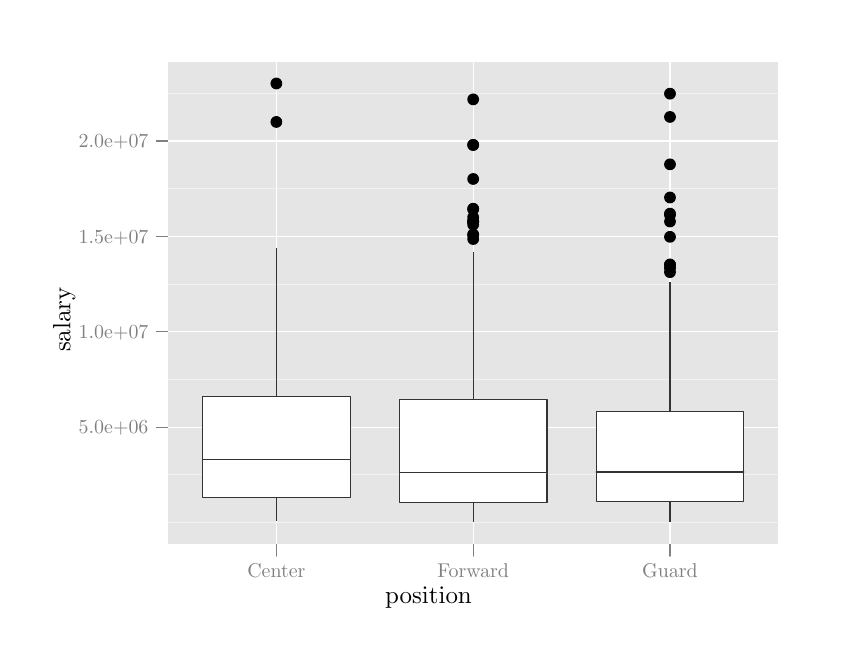
\begin{tikzpicture}[x=1pt,y=1pt]
\draw[color=white,opacity=0] (0,0) rectangle (289.08,216.81);
\begin{scope}
\path[clip] (  0.00,  0.00) rectangle (289.08,216.81);
\definecolor[named]{drawColor}{rgb}{0.82,0.31,0.27}
\end{scope}
\begin{scope}
\path[clip] (  0.00,  0.00) rectangle (289.08,216.81);
\definecolor[named]{drawColor}{rgb}{0.82,0.31,0.27}
\end{scope}
\begin{scope}
\path[clip] (  0.00,  0.00) rectangle (289.08,216.81);
\definecolor[named]{drawColor}{rgb}{0.82,0.31,0.27}
\end{scope}
\begin{scope}
\path[clip] (  0.00,  0.00) rectangle (289.08,216.81);
\definecolor[named]{drawColor}{rgb}{0.82,0.31,0.27}
\end{scope}
\begin{scope}
\path[clip] (  0.00,  0.00) rectangle (289.08,216.81);
\definecolor[named]{drawColor}{rgb}{0.82,0.31,0.27}
\end{scope}
\begin{scope}
\path[clip] (  0.00,  0.00) rectangle (289.08,216.81);
\definecolor[named]{drawColor}{rgb}{0.82,0.31,0.27}
\end{scope}
\begin{scope}
\path[clip] (  0.00,  0.00) rectangle (289.08,216.81);
\definecolor[named]{drawColor}{rgb}{0.82,0.31,0.27}
\end{scope}
\begin{scope}
\path[clip] (  0.00,  0.00) rectangle (289.08,216.81);
\definecolor[named]{drawColor}{rgb}{0.82,0.31,0.27}
\end{scope}
\begin{scope}
\path[clip] (  0.00,  0.00) rectangle (289.08,216.81);
\definecolor[named]{drawColor}{rgb}{0.82,0.31,0.27}
\definecolor[named]{fillColor}{rgb}{1.00,1.00,1.00}

\draw[fill=fillColor,draw opacity=0.00,] (  0.00,  0.00) rectangle (289.08,216.81);
\end{scope}
\begin{scope}
\path[clip] (  0.00,  0.00) rectangle (289.08,216.81);
\definecolor[named]{drawColor}{rgb}{0.82,0.31,0.27}
\end{scope}
\begin{scope}
\path[clip] (  0.00,  0.00) rectangle (289.08,216.81);
\definecolor[named]{drawColor}{rgb}{0.82,0.31,0.27}
\definecolor[named]{drawColor}{rgb}{0.00,0.00,0.00}

\node[color=drawColor,anchor=base,inner sep=0pt, outer sep=0pt, scale=  0.90] at (144.63,  9.03) {position%
};
\end{scope}
\begin{scope}
\path[clip] (  0.00,  0.00) rectangle (289.08,216.81);
\definecolor[named]{drawColor}{rgb}{0.82,0.31,0.27}
\definecolor[named]{drawColor}{rgb}{0.00,0.00,0.00}

\node[rotate= 90.00,color=drawColor,anchor=base,inner sep=0pt, outer sep=0pt, scale=  0.90] at ( 15.23,111.50) {salary%
};
\end{scope}
\begin{scope}
\path[clip] (  0.00,  0.00) rectangle (289.08,216.81);
\definecolor[named]{drawColor}{rgb}{0.82,0.31,0.27}
\end{scope}
\begin{scope}
\path[clip] ( 18.24,204.76) rectangle ( 50.55,204.76);
\definecolor[named]{drawColor}{rgb}{0.82,0.31,0.27}
\end{scope}
\begin{scope}
\path[clip] (  0.00,  0.00) rectangle (289.08,216.81);
\definecolor[named]{drawColor}{rgb}{0.82,0.31,0.27}
\end{scope}
\begin{scope}
\path[clip] ( 18.24,204.76) rectangle ( 50.55,204.76);
\definecolor[named]{drawColor}{rgb}{0.82,0.31,0.27}
\end{scope}
\begin{scope}
\path[clip] (  0.00,  0.00) rectangle (289.08,216.81);
\definecolor[named]{drawColor}{rgb}{0.82,0.31,0.27}
\end{scope}
\begin{scope}
\path[clip] (  0.00,  0.00) rectangle (289.08,216.81);
\definecolor[named]{drawColor}{rgb}{0.82,0.31,0.27}
\end{scope}
\begin{scope}
\path[clip] (  0.00,  0.00) rectangle (289.08,216.81);
\definecolor[named]{drawColor}{rgb}{0.82,0.31,0.27}
\end{scope}
\begin{scope}
\path[clip] ( 18.24, 30.32) rectangle ( 50.55, 30.32);
\definecolor[named]{drawColor}{rgb}{0.82,0.31,0.27}
\end{scope}
\begin{scope}
\path[clip] (  0.00,  0.00) rectangle (289.08,216.81);
\definecolor[named]{drawColor}{rgb}{0.82,0.31,0.27}
\end{scope}
\begin{scope}
\path[clip] ( 18.24, 18.24) rectangle ( 50.55, 30.32);
\definecolor[named]{drawColor}{rgb}{0.82,0.31,0.27}
\end{scope}
\begin{scope}
\path[clip] (  0.00,  0.00) rectangle (289.08,216.81);
\definecolor[named]{drawColor}{rgb}{0.82,0.31,0.27}
\end{scope}
\begin{scope}
\path[clip] ( 18.24, 18.24) rectangle ( 50.55, 18.24);
\definecolor[named]{drawColor}{rgb}{0.82,0.31,0.27}
\end{scope}
\begin{scope}
\path[clip] (  0.00,  0.00) rectangle (289.08,216.81);
\definecolor[named]{drawColor}{rgb}{0.82,0.31,0.27}
\end{scope}
\begin{scope}
\path[clip] ( 50.55,204.76) rectangle ( 50.55,204.76);
\definecolor[named]{drawColor}{rgb}{0.82,0.31,0.27}
\end{scope}
\begin{scope}
\path[clip] (  0.00,  0.00) rectangle (289.08,216.81);
\definecolor[named]{drawColor}{rgb}{0.82,0.31,0.27}
\end{scope}
\begin{scope}
\path[clip] ( 50.55,204.76) rectangle ( 50.55,204.76);
\definecolor[named]{drawColor}{rgb}{0.82,0.31,0.27}
\end{scope}
\begin{scope}
\path[clip] (  0.00,  0.00) rectangle (289.08,216.81);
\definecolor[named]{drawColor}{rgb}{0.82,0.31,0.27}
\end{scope}
\begin{scope}
\path[clip] ( 50.55, 30.32) rectangle ( 50.55,204.77);
\definecolor[named]{drawColor}{rgb}{0.82,0.31,0.27}
\end{scope}
\begin{scope}
\path[clip] (  0.00,  0.00) rectangle (289.08,216.81);
\definecolor[named]{drawColor}{rgb}{0.82,0.31,0.27}
\end{scope}
\begin{scope}
\path[clip] ( 50.55, 30.32) rectangle ( 50.55, 30.32);
\definecolor[named]{drawColor}{rgb}{0.82,0.31,0.27}
\end{scope}
\begin{scope}
\path[clip] (  0.00,  0.00) rectangle (289.08,216.81);
\definecolor[named]{drawColor}{rgb}{0.82,0.31,0.27}
\end{scope}
\begin{scope}
\path[clip] ( 50.55, 18.24) rectangle ( 50.55, 30.32);
\definecolor[named]{drawColor}{rgb}{0.82,0.31,0.27}
\end{scope}
\begin{scope}
\path[clip] (  0.00,  0.00) rectangle (289.08,216.81);
\definecolor[named]{drawColor}{rgb}{0.82,0.31,0.27}
\end{scope}
\begin{scope}
\path[clip] ( 50.55, 18.24) rectangle ( 50.55, 18.24);
\definecolor[named]{drawColor}{rgb}{0.82,0.31,0.27}
\end{scope}
\begin{scope}
\path[clip] (  0.00,  0.00) rectangle (289.08,216.81);
\definecolor[named]{drawColor}{rgb}{0.82,0.31,0.27}
\end{scope}
\begin{scope}
\path[clip] ( 50.55,204.76) rectangle (271.01,204.76);
\definecolor[named]{drawColor}{rgb}{0.82,0.31,0.27}
\end{scope}
\begin{scope}
\path[clip] (  0.00,  0.00) rectangle (289.08,216.81);
\definecolor[named]{drawColor}{rgb}{0.82,0.31,0.27}
\end{scope}
\begin{scope}
\path[clip] ( 50.55,204.76) rectangle (271.01,204.76);
\definecolor[named]{drawColor}{rgb}{0.82,0.31,0.27}
\end{scope}
\begin{scope}
\path[clip] (  0.00,  0.00) rectangle (289.08,216.81);
\definecolor[named]{drawColor}{rgb}{0.82,0.31,0.27}
\end{scope}
\begin{scope}
\path[clip] ( 50.55, 30.32) rectangle (271.01,204.77);
\definecolor[named]{drawColor}{rgb}{0.82,0.31,0.27}
\end{scope}
\begin{scope}
\path[clip] (  0.00,  0.00) rectangle (289.08,216.81);
\definecolor[named]{drawColor}{rgb}{0.82,0.31,0.27}
\end{scope}
\begin{scope}
\path[clip] ( 50.55, 30.32) rectangle (271.01, 30.32);
\definecolor[named]{drawColor}{rgb}{0.82,0.31,0.27}
\end{scope}
\begin{scope}
\path[clip] (  0.00,  0.00) rectangle (289.08,216.81);
\definecolor[named]{drawColor}{rgb}{0.82,0.31,0.27}
\end{scope}
\begin{scope}
\path[clip] (  0.00,  0.00) rectangle (289.08,216.81);
\definecolor[named]{drawColor}{rgb}{0.82,0.31,0.27}
\end{scope}
\begin{scope}
\path[clip] (  0.00,  0.00) rectangle (289.08,216.81);
\definecolor[named]{drawColor}{rgb}{0.82,0.31,0.27}
\end{scope}
\begin{scope}
\path[clip] ( 50.55, 18.24) rectangle (271.01, 18.24);
\definecolor[named]{drawColor}{rgb}{0.82,0.31,0.27}
\end{scope}
\begin{scope}
\path[clip] (  0.00,  0.00) rectangle (289.08,216.81);
\definecolor[named]{drawColor}{rgb}{0.82,0.31,0.27}
\end{scope}
\begin{scope}
\path[clip] (271.01,204.76) rectangle (271.01,204.76);
\definecolor[named]{drawColor}{rgb}{0.82,0.31,0.27}
\end{scope}
\begin{scope}
\path[clip] (  0.00,  0.00) rectangle (289.08,216.81);
\definecolor[named]{drawColor}{rgb}{0.82,0.31,0.27}
\end{scope}
\begin{scope}
\path[clip] (271.01,204.76) rectangle (271.01,204.76);
\definecolor[named]{drawColor}{rgb}{0.82,0.31,0.27}
\end{scope}
\begin{scope}
\path[clip] (  0.00,  0.00) rectangle (289.08,216.81);
\definecolor[named]{drawColor}{rgb}{0.82,0.31,0.27}
\end{scope}
\begin{scope}
\path[clip] (271.01, 30.32) rectangle (271.01,204.77);
\definecolor[named]{drawColor}{rgb}{0.82,0.31,0.27}
\end{scope}
\begin{scope}
\path[clip] (  0.00,  0.00) rectangle (289.08,216.81);
\definecolor[named]{drawColor}{rgb}{0.82,0.31,0.27}
\end{scope}
\begin{scope}
\path[clip] (271.01, 30.32) rectangle (271.01, 30.32);
\definecolor[named]{drawColor}{rgb}{0.82,0.31,0.27}
\end{scope}
\begin{scope}
\path[clip] (  0.00,  0.00) rectangle (289.08,216.81);
\definecolor[named]{drawColor}{rgb}{0.82,0.31,0.27}
\end{scope}
\begin{scope}
\path[clip] (271.01, 18.24) rectangle (271.01, 30.32);
\definecolor[named]{drawColor}{rgb}{0.82,0.31,0.27}
\end{scope}
\begin{scope}
\path[clip] (  0.00,  0.00) rectangle (289.08,216.81);
\definecolor[named]{drawColor}{rgb}{0.82,0.31,0.27}
\end{scope}
\begin{scope}
\path[clip] (271.01, 18.24) rectangle (271.01, 18.24);
\definecolor[named]{drawColor}{rgb}{0.82,0.31,0.27}
\end{scope}
\begin{scope}
\path[clip] (  0.00,  0.00) rectangle (289.08,216.81);
\definecolor[named]{drawColor}{rgb}{0.82,0.31,0.27}
\end{scope}
\begin{scope}
\path[clip] (271.01,204.76) rectangle (271.01,204.76);
\definecolor[named]{drawColor}{rgb}{0.82,0.31,0.27}
\end{scope}
\begin{scope}
\path[clip] (  0.00,  0.00) rectangle (289.08,216.81);
\definecolor[named]{drawColor}{rgb}{0.82,0.31,0.27}
\end{scope}
\begin{scope}
\path[clip] (271.01,204.76) rectangle (271.01,204.76);
\definecolor[named]{drawColor}{rgb}{0.82,0.31,0.27}
\end{scope}
\begin{scope}
\path[clip] (  0.00,  0.00) rectangle (289.08,216.81);
\definecolor[named]{drawColor}{rgb}{0.82,0.31,0.27}
\end{scope}
\begin{scope}
\path[clip] (271.01, 30.32) rectangle (271.01,204.77);
\definecolor[named]{drawColor}{rgb}{0.82,0.31,0.27}
\end{scope}
\begin{scope}
\path[clip] (  0.00,  0.00) rectangle (289.08,216.81);
\definecolor[named]{drawColor}{rgb}{0.82,0.31,0.27}
\end{scope}
\begin{scope}
\path[clip] (271.01, 30.32) rectangle (271.01, 30.32);
\definecolor[named]{drawColor}{rgb}{0.82,0.31,0.27}
\end{scope}
\begin{scope}
\path[clip] (  0.00,  0.00) rectangle (289.08,216.81);
\definecolor[named]{drawColor}{rgb}{0.82,0.31,0.27}
\end{scope}
\begin{scope}
\path[clip] (271.01, 18.24) rectangle (271.01, 30.32);
\definecolor[named]{drawColor}{rgb}{0.82,0.31,0.27}
\end{scope}
\begin{scope}
\path[clip] (  0.00,  0.00) rectangle (289.08,216.81);
\definecolor[named]{drawColor}{rgb}{0.82,0.31,0.27}
\end{scope}
\begin{scope}
\path[clip] (271.01, 18.24) rectangle (271.01, 18.24);
\definecolor[named]{drawColor}{rgb}{0.82,0.31,0.27}
\end{scope}
\begin{scope}
\path[clip] (  0.00,  0.00) rectangle (289.08,216.81);
\definecolor[named]{drawColor}{rgb}{0.82,0.31,0.27}
\end{scope}
\begin{scope}
\path[clip] (271.01,204.76) rectangle (271.01,204.76);
\definecolor[named]{drawColor}{rgb}{0.82,0.31,0.27}
\end{scope}
\begin{scope}
\path[clip] (  0.00,  0.00) rectangle (289.08,216.81);
\definecolor[named]{drawColor}{rgb}{0.82,0.31,0.27}
\end{scope}
\begin{scope}
\path[clip] (271.01,204.76) rectangle (271.01,204.76);
\definecolor[named]{drawColor}{rgb}{0.82,0.31,0.27}
\end{scope}
\begin{scope}
\path[clip] (  0.00,  0.00) rectangle (289.08,216.81);
\definecolor[named]{drawColor}{rgb}{0.82,0.31,0.27}
\end{scope}
\begin{scope}
\path[clip] (271.01, 30.32) rectangle (271.01,204.77);
\definecolor[named]{drawColor}{rgb}{0.82,0.31,0.27}
\end{scope}
\begin{scope}
\path[clip] (  0.00,  0.00) rectangle (289.08,216.81);
\definecolor[named]{drawColor}{rgb}{0.82,0.31,0.27}
\end{scope}
\begin{scope}
\path[clip] (271.01, 30.32) rectangle (271.01, 30.32);
\definecolor[named]{drawColor}{rgb}{0.82,0.31,0.27}
\end{scope}
\begin{scope}
\path[clip] (  0.00,  0.00) rectangle (289.08,216.81);
\definecolor[named]{drawColor}{rgb}{0.82,0.31,0.27}
\end{scope}
\begin{scope}
\path[clip] (271.01, 18.24) rectangle (271.01, 30.32);
\definecolor[named]{drawColor}{rgb}{0.82,0.31,0.27}
\end{scope}
\begin{scope}
\path[clip] (  0.00,  0.00) rectangle (289.08,216.81);
\definecolor[named]{drawColor}{rgb}{0.82,0.31,0.27}
\end{scope}
\begin{scope}
\path[clip] (271.01, 18.24) rectangle (271.01, 18.24);
\definecolor[named]{drawColor}{rgb}{0.82,0.31,0.27}
\end{scope}
\begin{scope}
\path[clip] (  0.00,  0.00) rectangle (289.08,216.81);
\definecolor[named]{drawColor}{rgb}{0.82,0.31,0.27}
\end{scope}
\begin{scope}
\path[clip] ( 18.24,204.76) rectangle ( 50.55,204.76);
\definecolor[named]{drawColor}{rgb}{0.82,0.31,0.27}
\end{scope}
\begin{scope}
\path[clip] (  0.00,  0.00) rectangle (289.08,216.81);
\definecolor[named]{drawColor}{rgb}{0.82,0.31,0.27}
\end{scope}
\begin{scope}
\path[clip] ( 18.24,204.76) rectangle ( 50.55,204.76);
\definecolor[named]{drawColor}{rgb}{0.82,0.31,0.27}
\end{scope}
\begin{scope}
\path[clip] (  0.00,  0.00) rectangle (289.08,216.81);
\definecolor[named]{drawColor}{rgb}{0.82,0.31,0.27}
\end{scope}
\begin{scope}
\path[clip] (  0.00,  0.00) rectangle (289.08,216.81);
\definecolor[named]{drawColor}{rgb}{0.82,0.31,0.27}
\definecolor[named]{drawColor}{rgb}{0.50,0.50,0.50}

\node[color=drawColor,anchor=base east,inner sep=0pt, outer sep=0pt, scale=  0.72] at ( 43.44, 70.20) {5.0e+06%
};

\node[color=drawColor,anchor=base east,inner sep=0pt, outer sep=0pt, scale=  0.72] at ( 43.44,104.66) {1.0e+07%
};

\node[color=drawColor,anchor=base east,inner sep=0pt, outer sep=0pt, scale=  0.72] at ( 43.44,139.12) {1.5e+07%
};

\node[color=drawColor,anchor=base east,inner sep=0pt, outer sep=0pt, scale=  0.72] at ( 43.44,173.57) {2.0e+07%
};
\end{scope}
\begin{scope}
\path[clip] (  0.00,  0.00) rectangle (289.08,216.81);
\definecolor[named]{drawColor}{rgb}{0.82,0.31,0.27}
\definecolor[named]{drawColor}{rgb}{0.50,0.50,0.50}

\draw[color=drawColor,line cap=round,line join=round,fill opacity=0.00,] ( 46.28, 72.68) -- ( 50.55, 72.68);

\draw[color=drawColor,line cap=round,line join=round,fill opacity=0.00,] ( 46.28,107.14) -- ( 50.55,107.14);

\draw[color=drawColor,line cap=round,line join=round,fill opacity=0.00,] ( 46.28,141.60) -- ( 50.55,141.60);

\draw[color=drawColor,line cap=round,line join=round,fill opacity=0.00,] ( 46.28,176.05) -- ( 50.55,176.05);
\end{scope}
\begin{scope}
\path[clip] (  0.00,  0.00) rectangle (289.08,216.81);
\definecolor[named]{drawColor}{rgb}{0.82,0.31,0.27}
\end{scope}
\begin{scope}
\path[clip] (  0.00,  0.00) rectangle (289.08,216.81);
\definecolor[named]{drawColor}{rgb}{0.82,0.31,0.27}
\end{scope}
\begin{scope}
\path[clip] (  0.00,  0.00) rectangle (289.08,216.81);
\definecolor[named]{drawColor}{rgb}{0.82,0.31,0.27}
\end{scope}
\begin{scope}
\path[clip] ( 18.24, 30.32) rectangle ( 50.55, 30.32);
\definecolor[named]{drawColor}{rgb}{0.82,0.31,0.27}
\end{scope}
\begin{scope}
\path[clip] (  0.00,  0.00) rectangle (289.08,216.81);
\definecolor[named]{drawColor}{rgb}{0.82,0.31,0.27}
\end{scope}
\begin{scope}
\path[clip] ( 18.24, 18.24) rectangle ( 50.55, 30.32);
\definecolor[named]{drawColor}{rgb}{0.82,0.31,0.27}
\end{scope}
\begin{scope}
\path[clip] (  0.00,  0.00) rectangle (289.08,216.81);
\definecolor[named]{drawColor}{rgb}{0.82,0.31,0.27}
\end{scope}
\begin{scope}
\path[clip] ( 18.24, 18.24) rectangle ( 50.55, 18.24);
\definecolor[named]{drawColor}{rgb}{0.82,0.31,0.27}
\end{scope}
\begin{scope}
\path[clip] (  0.00,  0.00) rectangle (289.08,216.81);
\definecolor[named]{drawColor}{rgb}{0.82,0.31,0.27}
\end{scope}
\begin{scope}
\path[clip] ( 50.55,204.76) rectangle ( 50.55,204.76);
\definecolor[named]{drawColor}{rgb}{0.82,0.31,0.27}
\end{scope}
\begin{scope}
\path[clip] (  0.00,  0.00) rectangle (289.08,216.81);
\definecolor[named]{drawColor}{rgb}{0.82,0.31,0.27}
\end{scope}
\begin{scope}
\path[clip] ( 50.55,204.76) rectangle ( 50.55,204.76);
\definecolor[named]{drawColor}{rgb}{0.82,0.31,0.27}
\end{scope}
\begin{scope}
\path[clip] (  0.00,  0.00) rectangle (289.08,216.81);
\definecolor[named]{drawColor}{rgb}{0.82,0.31,0.27}
\end{scope}
\begin{scope}
\path[clip] ( 50.55, 30.32) rectangle ( 50.55,204.77);
\definecolor[named]{drawColor}{rgb}{0.82,0.31,0.27}
\end{scope}
\begin{scope}
\path[clip] (  0.00,  0.00) rectangle (289.08,216.81);
\definecolor[named]{drawColor}{rgb}{0.82,0.31,0.27}
\end{scope}
\begin{scope}
\path[clip] ( 50.55, 30.32) rectangle ( 50.55, 30.32);
\definecolor[named]{drawColor}{rgb}{0.82,0.31,0.27}
\end{scope}
\begin{scope}
\path[clip] (  0.00,  0.00) rectangle (289.08,216.81);
\definecolor[named]{drawColor}{rgb}{0.82,0.31,0.27}
\end{scope}
\begin{scope}
\path[clip] ( 50.55, 18.24) rectangle ( 50.55, 30.32);
\definecolor[named]{drawColor}{rgb}{0.82,0.31,0.27}
\end{scope}
\begin{scope}
\path[clip] (  0.00,  0.00) rectangle (289.08,216.81);
\definecolor[named]{drawColor}{rgb}{0.82,0.31,0.27}
\end{scope}
\begin{scope}
\path[clip] ( 50.55, 18.24) rectangle ( 50.55, 18.24);
\definecolor[named]{drawColor}{rgb}{0.82,0.31,0.27}
\end{scope}
\begin{scope}
\path[clip] (  0.00,  0.00) rectangle (289.08,216.81);
\definecolor[named]{drawColor}{rgb}{0.82,0.31,0.27}
\end{scope}
\begin{scope}
\path[clip] ( 50.55,204.76) rectangle (271.01,204.76);
\definecolor[named]{drawColor}{rgb}{0.82,0.31,0.27}
\end{scope}
\begin{scope}
\path[clip] (  0.00,  0.00) rectangle (289.08,216.81);
\definecolor[named]{drawColor}{rgb}{0.82,0.31,0.27}
\end{scope}
\begin{scope}
\path[clip] ( 50.55,204.76) rectangle (271.01,204.76);
\definecolor[named]{drawColor}{rgb}{0.82,0.31,0.27}
\end{scope}
\begin{scope}
\path[clip] (  0.00,  0.00) rectangle (289.08,216.81);
\definecolor[named]{drawColor}{rgb}{0.82,0.31,0.27}
\end{scope}
\begin{scope}
\path[clip] ( 50.55, 30.32) rectangle (271.01,204.77);
\definecolor[named]{drawColor}{rgb}{0.82,0.31,0.27}
\definecolor[named]{fillColor}{rgb}{0.90,0.90,0.90}

\draw[fill=fillColor,draw opacity=0.00,] ( 50.55, 30.32) rectangle (271.01,204.77);
\definecolor[named]{drawColor}{rgb}{0.95,0.95,0.95}

\draw[color=drawColor,line width= 0.0pt,line cap=round,line join=round,fill opacity=0.00,] ( 50.55, 38.23) --
	(271.01, 38.23);

\draw[color=drawColor,line width= 0.0pt,line cap=round,line join=round,fill opacity=0.00,] ( 50.55, 55.45) --
	(271.01, 55.45);

\draw[color=drawColor,line width= 0.0pt,line cap=round,line join=round,fill opacity=0.00,] ( 50.55, 72.68) --
	(271.01, 72.68);

\draw[color=drawColor,line width= 0.0pt,line cap=round,line join=round,fill opacity=0.00,] ( 50.55, 89.91) --
	(271.01, 89.91);

\draw[color=drawColor,line width= 0.0pt,line cap=round,line join=round,fill opacity=0.00,] ( 50.55,107.14) --
	(271.01,107.14);

\draw[color=drawColor,line width= 0.0pt,line cap=round,line join=round,fill opacity=0.00,] ( 50.55,124.37) --
	(271.01,124.37);

\draw[color=drawColor,line width= 0.0pt,line cap=round,line join=round,fill opacity=0.00,] ( 50.55,141.60) --
	(271.01,141.60);

\draw[color=drawColor,line width= 0.0pt,line cap=round,line join=round,fill opacity=0.00,] ( 50.55,158.82) --
	(271.01,158.82);

\draw[color=drawColor,line width= 0.0pt,line cap=round,line join=round,fill opacity=0.00,] ( 50.55,176.05) --
	(271.01,176.05);

\draw[color=drawColor,line width= 0.0pt,line cap=round,line join=round,fill opacity=0.00,] ( 50.55,193.28) --
	(271.01,193.28);

\draw[color=drawColor,line width= 0.0pt,line cap=round,line join=round,fill opacity=0.00,] ( 89.66, 30.32) --
	( 89.66,204.77);

\draw[color=drawColor,line width= 0.0pt,line cap=round,line join=round,fill opacity=0.00,] (160.78, 30.32) --
	(160.78,204.77);

\draw[color=drawColor,line width= 0.0pt,line cap=round,line join=round,fill opacity=0.00,] (231.90, 30.32) --
	(231.90,204.77);
\definecolor[named]{drawColor}{rgb}{1.00,1.00,1.00}

\draw[color=drawColor,line cap=round,line join=round,fill opacity=0.00,] ( 50.55, 72.68) --
	(271.01, 72.68);

\draw[color=drawColor,line cap=round,line join=round,fill opacity=0.00,] ( 50.55,107.14) --
	(271.01,107.14);

\draw[color=drawColor,line cap=round,line join=round,fill opacity=0.00,] ( 50.55,141.60) --
	(271.01,141.60);

\draw[color=drawColor,line cap=round,line join=round,fill opacity=0.00,] ( 50.55,176.05) --
	(271.01,176.05);

\draw[color=drawColor,line cap=round,line join=round,fill opacity=0.00,] ( 89.66, 30.32) --
	( 89.66,204.77);

\draw[color=drawColor,line cap=round,line join=round,fill opacity=0.00,] (160.78, 30.32) --
	(160.78,204.77);

\draw[color=drawColor,line cap=round,line join=round,fill opacity=0.00,] (231.90, 30.32) --
	(231.90,204.77);
\definecolor[named]{fillColor}{rgb}{0.00,0.00,0.00}

\draw[fill=fillColor,draw opacity=0.00,] ( 89.66,196.84) circle (  2.13);

\draw[fill=fillColor,draw opacity=0.00,] ( 89.66,182.94) circle (  2.13);
\definecolor[named]{drawColor}{rgb}{0.20,0.20,0.20}

\draw[color=drawColor,line join=round,fill opacity=0.00,] ( 89.66, 83.78) --
	( 89.66,137.53);

\draw[color=drawColor,line join=round,fill opacity=0.00,] ( 89.66, 47.23) --
	( 89.66, 38.78);
\definecolor[named]{fillColor}{rgb}{1.00,1.00,1.00}

\draw[color=drawColor,line join=round,fill=fillColor,] ( 63.00, 47.23) rectangle (116.33, 83.78);

\draw[color=drawColor,line join=round,fill=fillColor,] ( 63.00, 60.99) rectangle (116.33, 60.99);
\definecolor[named]{fillColor}{rgb}{0.00,0.00,0.00}

\draw[fill=fillColor,draw opacity=0.00,] (160.78,146.97) circle (  2.13);

\draw[fill=fillColor,draw opacity=0.00,] (160.78,146.97) circle (  2.13);

\draw[fill=fillColor,draw opacity=0.00,] (160.78,140.62) circle (  2.13);

\draw[fill=fillColor,draw opacity=0.00,] (160.78,191.10) circle (  2.13);

\draw[fill=fillColor,draw opacity=0.00,] (160.78,151.36) circle (  2.13);

\draw[fill=fillColor,draw opacity=0.00,] (160.78,142.33) circle (  2.13);

\draw[fill=fillColor,draw opacity=0.00,] (160.78,146.97) circle (  2.13);

\draw[fill=fillColor,draw opacity=0.00,] (160.78,151.60) circle (  2.13);

\draw[fill=fillColor,draw opacity=0.00,] (160.78,162.34) circle (  2.13);

\draw[fill=fillColor,draw opacity=0.00,] (160.78,145.82) circle (  2.13);

\draw[fill=fillColor,draw opacity=0.00,] (160.78,174.64) circle (  2.13);

\draw[fill=fillColor,draw opacity=0.00,] (160.78,174.64) circle (  2.13);

\draw[fill=fillColor,draw opacity=0.00,] (160.78,148.49) circle (  2.13);

\draw[fill=fillColor,draw opacity=0.00,] (160.78,142.08) circle (  2.13);

\draw[color=drawColor,line join=round,fill opacity=0.00,] (160.78, 82.80) --
	(160.78,136.08);

\draw[color=drawColor,line join=round,fill opacity=0.00,] (160.78, 45.39) --
	(160.78, 38.41);
\definecolor[named]{fillColor}{rgb}{1.00,1.00,1.00}

\draw[color=drawColor,line join=round,fill=fillColor,] (134.11, 45.39) rectangle (187.45, 82.80);

\draw[color=drawColor,line join=round,fill=fillColor,] (134.11, 56.13) rectangle (187.45, 56.13);
\definecolor[named]{fillColor}{rgb}{0.00,0.00,0.00}

\draw[fill=fillColor,draw opacity=0.00,] (231.90,167.62) circle (  2.13);

\draw[fill=fillColor,draw opacity=0.00,] (231.90,149.81) circle (  2.13);

\draw[fill=fillColor,draw opacity=0.00,] (231.90,184.75) circle (  2.13);

\draw[fill=fillColor,draw opacity=0.00,] (231.90,149.34) circle (  2.13);

\draw[fill=fillColor,draw opacity=0.00,] (231.90,141.43) circle (  2.13);

\draw[fill=fillColor,draw opacity=0.00,] (231.90,193.16) circle (  2.13);

\draw[fill=fillColor,draw opacity=0.00,] (231.90,128.67) circle (  2.13);

\draw[fill=fillColor,draw opacity=0.00,] (231.90,131.40) circle (  2.13);

\draw[fill=fillColor,draw opacity=0.00,] (231.90,155.65) circle (  2.13);

\draw[fill=fillColor,draw opacity=0.00,] (231.90,130.11) circle (  2.13);

\draw[fill=fillColor,draw opacity=0.00,] (231.90,146.97) circle (  2.13);

\draw[fill=fillColor,draw opacity=0.00,] (231.90,131.40) circle (  2.13);

\draw[color=drawColor,line join=round,fill opacity=0.00,] (231.90, 78.20) --
	(231.90,125.06);

\draw[color=drawColor,line join=round,fill opacity=0.00,] (231.90, 45.71) --
	(231.90, 38.24);
\definecolor[named]{fillColor}{rgb}{1.00,1.00,1.00}

\draw[color=drawColor,line join=round,fill=fillColor,] (205.23, 45.71) rectangle (258.57, 78.20);

\draw[color=drawColor,line join=round,fill=fillColor,] (205.23, 56.45) rectangle (258.57, 56.45);
\end{scope}
\begin{scope}
\path[clip] (  0.00,  0.00) rectangle (289.08,216.81);
\definecolor[named]{drawColor}{rgb}{0.82,0.31,0.27}
\end{scope}
\begin{scope}
\path[clip] ( 50.55, 30.32) rectangle (271.01, 30.32);
\definecolor[named]{drawColor}{rgb}{0.82,0.31,0.27}
\end{scope}
\begin{scope}
\path[clip] (  0.00,  0.00) rectangle (289.08,216.81);
\definecolor[named]{drawColor}{rgb}{0.82,0.31,0.27}
\end{scope}
\begin{scope}
\path[clip] (  0.00,  0.00) rectangle (289.08,216.81);
\definecolor[named]{drawColor}{rgb}{0.82,0.31,0.27}
\definecolor[named]{drawColor}{rgb}{0.50,0.50,0.50}

\node[color=drawColor,anchor=base,inner sep=0pt, outer sep=0pt, scale=  0.72] at ( 89.66, 18.24) {Center%
};

\node[color=drawColor,anchor=base,inner sep=0pt, outer sep=0pt, scale=  0.72] at (160.78, 18.24) {Forward%
};

\node[color=drawColor,anchor=base,inner sep=0pt, outer sep=0pt, scale=  0.72] at (231.90, 18.24) {Guard%
};
\end{scope}
\begin{scope}
\path[clip] (  0.00,  0.00) rectangle (289.08,216.81);
\definecolor[named]{drawColor}{rgb}{0.82,0.31,0.27}
\definecolor[named]{drawColor}{rgb}{0.50,0.50,0.50}

\draw[color=drawColor,line cap=round,line join=round,fill opacity=0.00,] ( 89.66, 26.05) -- ( 89.66, 30.32);

\draw[color=drawColor,line cap=round,line join=round,fill opacity=0.00,] (160.78, 26.05) -- (160.78, 30.32);

\draw[color=drawColor,line cap=round,line join=round,fill opacity=0.00,] (231.90, 26.05) -- (231.90, 30.32);
\end{scope}
\begin{scope}
\path[clip] (  0.00,  0.00) rectangle (289.08,216.81);
\definecolor[named]{drawColor}{rgb}{0.82,0.31,0.27}
\end{scope}
\begin{scope}
\path[clip] (  0.00,  0.00) rectangle (289.08,216.81);
\definecolor[named]{drawColor}{rgb}{0.82,0.31,0.27}
\end{scope}
\begin{scope}
\path[clip] (  0.00,  0.00) rectangle (289.08,216.81);
\definecolor[named]{drawColor}{rgb}{0.82,0.31,0.27}
\end{scope}
\begin{scope}
\path[clip] ( 50.55, 18.24) rectangle (271.01, 18.24);
\definecolor[named]{drawColor}{rgb}{0.82,0.31,0.27}
\end{scope}
\begin{scope}
\path[clip] (  0.00,  0.00) rectangle (289.08,216.81);
\definecolor[named]{drawColor}{rgb}{0.82,0.31,0.27}
\end{scope}
\begin{scope}
\path[clip] (271.01,204.76) rectangle (271.01,204.76);
\definecolor[named]{drawColor}{rgb}{0.82,0.31,0.27}
\end{scope}
\begin{scope}
\path[clip] (  0.00,  0.00) rectangle (289.08,216.81);
\definecolor[named]{drawColor}{rgb}{0.82,0.31,0.27}
\end{scope}
\begin{scope}
\path[clip] (271.01,204.76) rectangle (271.01,204.76);
\definecolor[named]{drawColor}{rgb}{0.82,0.31,0.27}
\end{scope}
\begin{scope}
\path[clip] (  0.00,  0.00) rectangle (289.08,216.81);
\definecolor[named]{drawColor}{rgb}{0.82,0.31,0.27}
\end{scope}
\begin{scope}
\path[clip] (271.01, 30.32) rectangle (271.01,204.77);
\definecolor[named]{drawColor}{rgb}{0.82,0.31,0.27}
\end{scope}
\begin{scope}
\path[clip] (  0.00,  0.00) rectangle (289.08,216.81);
\definecolor[named]{drawColor}{rgb}{0.82,0.31,0.27}
\end{scope}
\begin{scope}
\path[clip] (271.01, 30.32) rectangle (271.01, 30.32);
\definecolor[named]{drawColor}{rgb}{0.82,0.31,0.27}
\end{scope}
\begin{scope}
\path[clip] (  0.00,  0.00) rectangle (289.08,216.81);
\definecolor[named]{drawColor}{rgb}{0.82,0.31,0.27}
\end{scope}
\begin{scope}
\path[clip] (271.01, 18.24) rectangle (271.01, 30.32);
\definecolor[named]{drawColor}{rgb}{0.82,0.31,0.27}
\end{scope}
\begin{scope}
\path[clip] (  0.00,  0.00) rectangle (289.08,216.81);
\definecolor[named]{drawColor}{rgb}{0.82,0.31,0.27}
\end{scope}
\begin{scope}
\path[clip] (271.01, 18.24) rectangle (271.01, 18.24);
\definecolor[named]{drawColor}{rgb}{0.82,0.31,0.27}
\end{scope}
\begin{scope}
\path[clip] (  0.00,  0.00) rectangle (289.08,216.81);
\definecolor[named]{drawColor}{rgb}{0.82,0.31,0.27}
\end{scope}
\begin{scope}
\path[clip] (271.01,204.76) rectangle (271.01,204.76);
\definecolor[named]{drawColor}{rgb}{0.82,0.31,0.27}
\end{scope}
\begin{scope}
\path[clip] (  0.00,  0.00) rectangle (289.08,216.81);
\definecolor[named]{drawColor}{rgb}{0.82,0.31,0.27}
\end{scope}
\begin{scope}
\path[clip] (271.01,204.76) rectangle (271.01,204.76);
\definecolor[named]{drawColor}{rgb}{0.82,0.31,0.27}
\end{scope}
\begin{scope}
\path[clip] (  0.00,  0.00) rectangle (289.08,216.81);
\definecolor[named]{drawColor}{rgb}{0.82,0.31,0.27}
\end{scope}
\begin{scope}
\path[clip] (271.01, 30.32) rectangle (271.01,204.77);
\definecolor[named]{drawColor}{rgb}{0.82,0.31,0.27}
\end{scope}
\begin{scope}
\path[clip] (  0.00,  0.00) rectangle (289.08,216.81);
\definecolor[named]{drawColor}{rgb}{0.82,0.31,0.27}
\end{scope}
\begin{scope}
\path[clip] (271.01, 30.32) rectangle (271.01, 30.32);
\definecolor[named]{drawColor}{rgb}{0.82,0.31,0.27}
\end{scope}
\begin{scope}
\path[clip] (  0.00,  0.00) rectangle (289.08,216.81);
\definecolor[named]{drawColor}{rgb}{0.82,0.31,0.27}
\end{scope}
\begin{scope}
\path[clip] (271.01, 18.24) rectangle (271.01, 30.32);
\definecolor[named]{drawColor}{rgb}{0.82,0.31,0.27}
\end{scope}
\begin{scope}
\path[clip] (  0.00,  0.00) rectangle (289.08,216.81);
\definecolor[named]{drawColor}{rgb}{0.82,0.31,0.27}
\end{scope}
\begin{scope}
\path[clip] (271.01, 18.24) rectangle (271.01, 18.24);
\definecolor[named]{drawColor}{rgb}{0.82,0.31,0.27}
\end{scope}
\begin{scope}
\path[clip] (  0.00,  0.00) rectangle (289.08,216.81);
\definecolor[named]{drawColor}{rgb}{0.82,0.31,0.27}
\end{scope}
\begin{scope}
\path[clip] (271.01,204.76) rectangle (271.01,204.76);
\definecolor[named]{drawColor}{rgb}{0.82,0.31,0.27}
\end{scope}
\begin{scope}
\path[clip] (  0.00,  0.00) rectangle (289.08,216.81);
\definecolor[named]{drawColor}{rgb}{0.82,0.31,0.27}
\end{scope}
\begin{scope}
\path[clip] (271.01,204.76) rectangle (271.01,204.76);
\definecolor[named]{drawColor}{rgb}{0.82,0.31,0.27}
\end{scope}
\begin{scope}
\path[clip] (  0.00,  0.00) rectangle (289.08,216.81);
\definecolor[named]{drawColor}{rgb}{0.82,0.31,0.27}
\end{scope}
\begin{scope}
\path[clip] (271.01, 30.32) rectangle (271.01,204.77);
\definecolor[named]{drawColor}{rgb}{0.82,0.31,0.27}
\end{scope}
\begin{scope}
\path[clip] (  0.00,  0.00) rectangle (289.08,216.81);
\definecolor[named]{drawColor}{rgb}{0.82,0.31,0.27}
\end{scope}
\begin{scope}
\path[clip] (271.01, 30.32) rectangle (271.01, 30.32);
\definecolor[named]{drawColor}{rgb}{0.82,0.31,0.27}
\end{scope}
\begin{scope}
\path[clip] (  0.00,  0.00) rectangle (289.08,216.81);
\definecolor[named]{drawColor}{rgb}{0.82,0.31,0.27}
\end{scope}
\begin{scope}
\path[clip] (271.01, 18.24) rectangle (271.01, 30.32);
\definecolor[named]{drawColor}{rgb}{0.82,0.31,0.27}
\end{scope}
\begin{scope}
\path[clip] (  0.00,  0.00) rectangle (289.08,216.81);
\definecolor[named]{drawColor}{rgb}{0.82,0.31,0.27}
\end{scope}
\begin{scope}
\path[clip] (271.01, 18.24) rectangle (271.01, 18.24);
\definecolor[named]{drawColor}{rgb}{0.82,0.31,0.27}
\end{scope}
\begin{scope}
\path[clip] (  0.00,  0.00) rectangle (289.08,216.81);
\definecolor[named]{drawColor}{rgb}{0.82,0.31,0.27}
\end{scope}
\begin{scope}
\path[clip] (  0.00,  0.00) rectangle (289.08,216.81);
\definecolor[named]{drawColor}{rgb}{0.82,0.31,0.27}
\end{scope}
\begin{scope}
\path[clip] (  0.00,  0.00) rectangle (289.08,216.81);
\definecolor[named]{drawColor}{rgb}{0.82,0.31,0.27}
\end{scope}
\end{tikzpicture}

\endpgfgraphicnamed
\end{center}
\end{dummy}
\caption{Salaries for different positions: the \texttt{Center} seems to have
better salaries.\label{fig:salary-position}}

\end{figure}


%
\begin{figure}
\begin{dummy}
\hspace*{\fill}\\
\hlstd{}\ttfamily\noindent
\hlprompt{\usebox{\hlnormalsizeboxgreaterthan}{\ }}\hlfunctioncall{print}\hlkeyword{(}\hlfunctioncall{qplot}\hlkeyword{(}\hlsymbol{minutes}\hlkeyword{/}\hlsymbol{gp}\hlkeyword{,}{\ }\hlfunctioncall{log}\hlkeyword{(}\hlsymbol{salary}\hlkeyword{)}\hlkeyword{,}{\ }\hlargument{data}{\ }\hlargument{=}{\ }\hlsymbol{bb}\hlkeyword{,}{\ }\hlargument{facets}{\ }\hlargument{=}{\ }\hlsymbol{position}{\ }\hlkeyword{\urltilda{}}\hspace*{\fill}\\
\hlstd{}\hlprompt{+{\ }}{\ }{\ }{\ }{\ }\hlsymbol{.}\hlkeyword{,}{\ }\hlargument{geom}{\ }\hlargument{=}{\ }\hlfunctioncall{c}\hlkeyword{(}\hlstring{"point"}\hlkeyword{,}{\ }\hlstring{"smooth"}\hlkeyword{)}\hlkeyword{)}\hlkeyword{)}\mbox{}
\normalfont
\hspace*{\fill}\\
\hlstd{}
\begin{center}

\beginpgfgraphicnamed{figure/Rfig-salary-minpergp}
% Created by tikzDevice version 0.5.3 on 2011-01-28 19:54:38
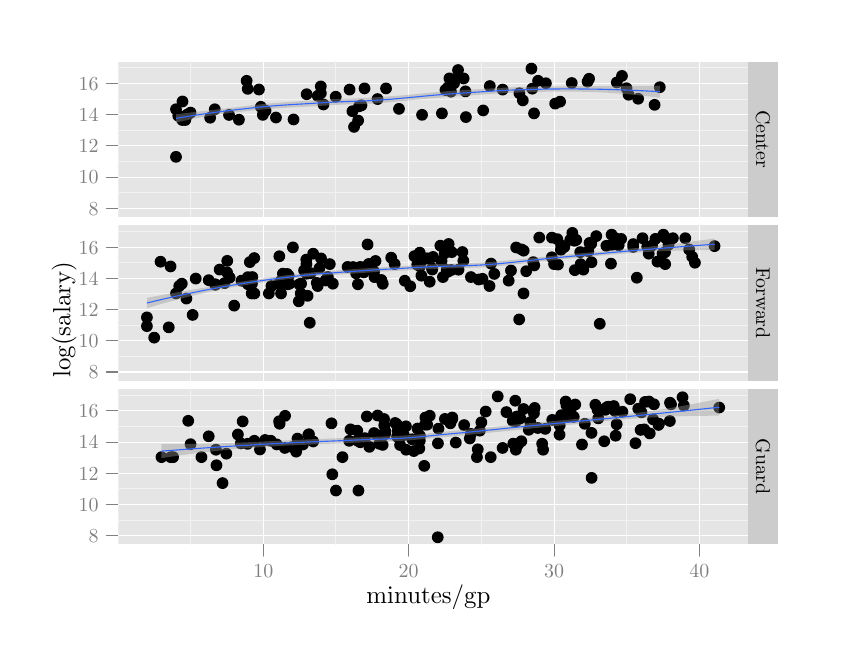
\begin{tikzpicture}[x=1pt,y=1pt]
\draw[color=white,opacity=0] (0,0) rectangle (289.08,216.81);
\begin{scope}
\path[clip] (  0.00,  0.00) rectangle (289.08,216.81);
\definecolor[named]{drawColor}{rgb}{0.19,0.40,0.69}
\end{scope}
\begin{scope}
\path[clip] (  0.00,  0.00) rectangle (289.08,216.81);
\definecolor[named]{drawColor}{rgb}{0.19,0.40,0.69}
\end{scope}
\begin{scope}
\path[clip] (  0.00,  0.00) rectangle (289.08,216.81);
\definecolor[named]{drawColor}{rgb}{0.19,0.40,0.69}
\end{scope}
\begin{scope}
\path[clip] (  0.00,  0.00) rectangle (289.08,216.81);
\definecolor[named]{drawColor}{rgb}{0.19,0.40,0.69}
\end{scope}
\begin{scope}
\path[clip] (  0.00,  0.00) rectangle (289.08,216.81);
\definecolor[named]{drawColor}{rgb}{0.19,0.40,0.69}
\end{scope}
\begin{scope}
\path[clip] (  0.00,  0.00) rectangle (289.08,216.81);
\definecolor[named]{drawColor}{rgb}{0.19,0.40,0.69}
\end{scope}
\begin{scope}
\path[clip] (  0.00,  0.00) rectangle (289.08,216.81);
\definecolor[named]{drawColor}{rgb}{0.19,0.40,0.69}
\end{scope}
\begin{scope}
\path[clip] (  0.00,  0.00) rectangle (289.08,216.81);
\definecolor[named]{drawColor}{rgb}{0.19,0.40,0.69}
\end{scope}
\begin{scope}
\path[clip] (  0.00,  0.00) rectangle (289.08,216.81);
\definecolor[named]{drawColor}{rgb}{0.19,0.40,0.69}
\end{scope}
\begin{scope}
\path[clip] (  0.00,  0.00) rectangle (289.08,216.81);
\definecolor[named]{drawColor}{rgb}{0.19,0.40,0.69}
\end{scope}
\begin{scope}
\path[clip] (  0.00,  0.00) rectangle (289.08,216.81);
\definecolor[named]{drawColor}{rgb}{0.19,0.40,0.69}
\definecolor[named]{fillColor}{rgb}{1.00,1.00,1.00}

\draw[fill=fillColor,draw opacity=0.00,] (  0.00,  0.00) rectangle (289.08,216.81);
\end{scope}
\begin{scope}
\path[clip] (  0.00,  0.00) rectangle (289.08,216.81);
\definecolor[named]{drawColor}{rgb}{0.19,0.40,0.69}
\end{scope}
\begin{scope}
\path[clip] (  0.00,  0.00) rectangle (289.08,216.81);
\definecolor[named]{drawColor}{rgb}{0.19,0.40,0.69}
\definecolor[named]{drawColor}{rgb}{0.00,0.00,0.00}

\node[color=drawColor,anchor=base,inner sep=0pt, outer sep=0pt, scale=  0.90] at (144.63,  9.03) {minutes/gp%
};
\end{scope}
\begin{scope}
\path[clip] (  0.00,  0.00) rectangle (289.08,216.81);
\definecolor[named]{drawColor}{rgb}{0.19,0.40,0.69}
\definecolor[named]{drawColor}{rgb}{0.00,0.00,0.00}

\node[rotate= 90.00,color=drawColor,anchor=base,inner sep=0pt, outer sep=0pt, scale=  0.90] at ( 15.23,111.50) {log(salary)%
};
\end{scope}
\begin{scope}
\path[clip] (  0.00,  0.00) rectangle (289.08,216.81);
\definecolor[named]{drawColor}{rgb}{0.19,0.40,0.69}
\end{scope}
\begin{scope}
\path[clip] ( 18.24,204.76) rectangle ( 32.55,204.76);
\definecolor[named]{drawColor}{rgb}{0.19,0.40,0.69}
\end{scope}
\begin{scope}
\path[clip] (  0.00,  0.00) rectangle (289.08,216.81);
\definecolor[named]{drawColor}{rgb}{0.19,0.40,0.69}
\end{scope}
\begin{scope}
\path[clip] ( 18.24,204.76) rectangle ( 32.55,204.76);
\definecolor[named]{drawColor}{rgb}{0.19,0.40,0.69}
\end{scope}
\begin{scope}
\path[clip] (  0.00,  0.00) rectangle (289.08,216.81);
\definecolor[named]{drawColor}{rgb}{0.19,0.40,0.69}
\end{scope}
\begin{scope}
\path[clip] (  0.00,  0.00) rectangle (289.08,216.81);
\definecolor[named]{drawColor}{rgb}{0.19,0.40,0.69}
\end{scope}
\begin{scope}
\path[clip] (  0.00,  0.00) rectangle (289.08,216.81);
\definecolor[named]{drawColor}{rgb}{0.19,0.40,0.69}
\end{scope}
\begin{scope}
\path[clip] ( 18.24,145.61) rectangle ( 32.55,148.62);
\definecolor[named]{drawColor}{rgb}{0.19,0.40,0.69}
\end{scope}
\begin{scope}
\path[clip] (  0.00,  0.00) rectangle (289.08,216.81);
\definecolor[named]{drawColor}{rgb}{0.19,0.40,0.69}
\end{scope}
\begin{scope}
\path[clip] (  0.00,  0.00) rectangle (289.08,216.81);
\definecolor[named]{drawColor}{rgb}{0.19,0.40,0.69}
\end{scope}
\begin{scope}
\path[clip] (  0.00,  0.00) rectangle (289.08,216.81);
\definecolor[named]{drawColor}{rgb}{0.19,0.40,0.69}
\end{scope}
\begin{scope}
\path[clip] ( 18.24, 86.46) rectangle ( 32.55, 89.47);
\definecolor[named]{drawColor}{rgb}{0.19,0.40,0.69}
\end{scope}
\begin{scope}
\path[clip] (  0.00,  0.00) rectangle (289.08,216.81);
\definecolor[named]{drawColor}{rgb}{0.19,0.40,0.69}
\end{scope}
\begin{scope}
\path[clip] (  0.00,  0.00) rectangle (289.08,216.81);
\definecolor[named]{drawColor}{rgb}{0.19,0.40,0.69}
\end{scope}
\begin{scope}
\path[clip] (  0.00,  0.00) rectangle (289.08,216.81);
\definecolor[named]{drawColor}{rgb}{0.19,0.40,0.69}
\end{scope}
\begin{scope}
\path[clip] ( 18.24, 30.32) rectangle ( 32.55, 30.32);
\definecolor[named]{drawColor}{rgb}{0.19,0.40,0.69}
\end{scope}
\begin{scope}
\path[clip] (  0.00,  0.00) rectangle (289.08,216.81);
\definecolor[named]{drawColor}{rgb}{0.19,0.40,0.69}
\end{scope}
\begin{scope}
\path[clip] ( 18.24, 18.24) rectangle ( 32.55, 30.32);
\definecolor[named]{drawColor}{rgb}{0.19,0.40,0.69}
\end{scope}
\begin{scope}
\path[clip] (  0.00,  0.00) rectangle (289.08,216.81);
\definecolor[named]{drawColor}{rgb}{0.19,0.40,0.69}
\end{scope}
\begin{scope}
\path[clip] ( 18.24, 18.24) rectangle ( 32.55, 18.24);
\definecolor[named]{drawColor}{rgb}{0.19,0.40,0.69}
\end{scope}
\begin{scope}
\path[clip] (  0.00,  0.00) rectangle (289.08,216.81);
\definecolor[named]{drawColor}{rgb}{0.19,0.40,0.69}
\end{scope}
\begin{scope}
\path[clip] ( 32.55,204.76) rectangle ( 32.55,204.76);
\definecolor[named]{drawColor}{rgb}{0.19,0.40,0.69}
\end{scope}
\begin{scope}
\path[clip] (  0.00,  0.00) rectangle (289.08,216.81);
\definecolor[named]{drawColor}{rgb}{0.19,0.40,0.69}
\end{scope}
\begin{scope}
\path[clip] ( 32.55,204.76) rectangle ( 32.55,204.76);
\definecolor[named]{drawColor}{rgb}{0.19,0.40,0.69}
\end{scope}
\begin{scope}
\path[clip] (  0.00,  0.00) rectangle (289.08,216.81);
\definecolor[named]{drawColor}{rgb}{0.19,0.40,0.69}
\end{scope}
\begin{scope}
\path[clip] ( 32.55,148.62) rectangle ( 32.55,204.77);
\definecolor[named]{drawColor}{rgb}{0.19,0.40,0.69}
\end{scope}
\begin{scope}
\path[clip] (  0.00,  0.00) rectangle (289.08,216.81);
\definecolor[named]{drawColor}{rgb}{0.19,0.40,0.69}
\end{scope}
\begin{scope}
\path[clip] ( 32.55,145.61) rectangle ( 32.55,148.62);
\definecolor[named]{drawColor}{rgb}{0.19,0.40,0.69}
\end{scope}
\begin{scope}
\path[clip] (  0.00,  0.00) rectangle (289.08,216.81);
\definecolor[named]{drawColor}{rgb}{0.19,0.40,0.69}
\end{scope}
\begin{scope}
\path[clip] ( 32.55, 89.47) rectangle ( 32.55,145.61);
\definecolor[named]{drawColor}{rgb}{0.19,0.40,0.69}
\end{scope}
\begin{scope}
\path[clip] (  0.00,  0.00) rectangle (289.08,216.81);
\definecolor[named]{drawColor}{rgb}{0.19,0.40,0.69}
\end{scope}
\begin{scope}
\path[clip] ( 32.55, 86.46) rectangle ( 32.55, 89.47);
\definecolor[named]{drawColor}{rgb}{0.19,0.40,0.69}
\end{scope}
\begin{scope}
\path[clip] (  0.00,  0.00) rectangle (289.08,216.81);
\definecolor[named]{drawColor}{rgb}{0.19,0.40,0.69}
\end{scope}
\begin{scope}
\path[clip] ( 32.55, 30.32) rectangle ( 32.55, 86.46);
\definecolor[named]{drawColor}{rgb}{0.19,0.40,0.69}
\end{scope}
\begin{scope}
\path[clip] (  0.00,  0.00) rectangle (289.08,216.81);
\definecolor[named]{drawColor}{rgb}{0.19,0.40,0.69}
\end{scope}
\begin{scope}
\path[clip] ( 32.55, 30.32) rectangle ( 32.55, 30.32);
\definecolor[named]{drawColor}{rgb}{0.19,0.40,0.69}
\end{scope}
\begin{scope}
\path[clip] (  0.00,  0.00) rectangle (289.08,216.81);
\definecolor[named]{drawColor}{rgb}{0.19,0.40,0.69}
\end{scope}
\begin{scope}
\path[clip] ( 32.55, 18.24) rectangle ( 32.55, 30.32);
\definecolor[named]{drawColor}{rgb}{0.19,0.40,0.69}
\end{scope}
\begin{scope}
\path[clip] (  0.00,  0.00) rectangle (289.08,216.81);
\definecolor[named]{drawColor}{rgb}{0.19,0.40,0.69}
\end{scope}
\begin{scope}
\path[clip] ( 32.55, 18.24) rectangle ( 32.55, 18.24);
\definecolor[named]{drawColor}{rgb}{0.19,0.40,0.69}
\end{scope}
\begin{scope}
\path[clip] (  0.00,  0.00) rectangle (289.08,216.81);
\definecolor[named]{drawColor}{rgb}{0.19,0.40,0.69}
\end{scope}
\begin{scope}
\path[clip] ( 32.55,204.76) rectangle (260.03,204.76);
\definecolor[named]{drawColor}{rgb}{0.19,0.40,0.69}
\end{scope}
\begin{scope}
\path[clip] (  0.00,  0.00) rectangle (289.08,216.81);
\definecolor[named]{drawColor}{rgb}{0.19,0.40,0.69}
\end{scope}
\begin{scope}
\path[clip] ( 32.55,204.76) rectangle (260.03,204.76);
\definecolor[named]{drawColor}{rgb}{0.19,0.40,0.69}
\end{scope}
\begin{scope}
\path[clip] (  0.00,  0.00) rectangle (289.08,216.81);
\definecolor[named]{drawColor}{rgb}{0.19,0.40,0.69}
\end{scope}
\begin{scope}
\path[clip] ( 32.55,148.62) rectangle (260.03,204.77);
\definecolor[named]{drawColor}{rgb}{0.19,0.40,0.69}
\end{scope}
\begin{scope}
\path[clip] (  0.00,  0.00) rectangle (289.08,216.81);
\definecolor[named]{drawColor}{rgb}{0.19,0.40,0.69}
\end{scope}
\begin{scope}
\path[clip] ( 32.55,145.61) rectangle (260.03,148.62);
\definecolor[named]{drawColor}{rgb}{0.19,0.40,0.69}
\end{scope}
\begin{scope}
\path[clip] (  0.00,  0.00) rectangle (289.08,216.81);
\definecolor[named]{drawColor}{rgb}{0.19,0.40,0.69}
\end{scope}
\begin{scope}
\path[clip] ( 32.55, 89.47) rectangle (260.03,145.61);
\definecolor[named]{drawColor}{rgb}{0.19,0.40,0.69}
\end{scope}
\begin{scope}
\path[clip] (  0.00,  0.00) rectangle (289.08,216.81);
\definecolor[named]{drawColor}{rgb}{0.19,0.40,0.69}
\end{scope}
\begin{scope}
\path[clip] ( 32.55, 86.46) rectangle (260.03, 89.47);
\definecolor[named]{drawColor}{rgb}{0.19,0.40,0.69}
\end{scope}
\begin{scope}
\path[clip] (  0.00,  0.00) rectangle (289.08,216.81);
\definecolor[named]{drawColor}{rgb}{0.19,0.40,0.69}
\end{scope}
\begin{scope}
\path[clip] ( 32.55, 30.32) rectangle (260.03, 86.46);
\definecolor[named]{drawColor}{rgb}{0.19,0.40,0.69}
\end{scope}
\begin{scope}
\path[clip] (  0.00,  0.00) rectangle (289.08,216.81);
\definecolor[named]{drawColor}{rgb}{0.19,0.40,0.69}
\end{scope}
\begin{scope}
\path[clip] ( 32.55, 30.32) rectangle (260.03, 30.32);
\definecolor[named]{drawColor}{rgb}{0.19,0.40,0.69}
\end{scope}
\begin{scope}
\path[clip] (  0.00,  0.00) rectangle (289.08,216.81);
\definecolor[named]{drawColor}{rgb}{0.19,0.40,0.69}
\end{scope}
\begin{scope}
\path[clip] (  0.00,  0.00) rectangle (289.08,216.81);
\definecolor[named]{drawColor}{rgb}{0.19,0.40,0.69}
\end{scope}
\begin{scope}
\path[clip] (  0.00,  0.00) rectangle (289.08,216.81);
\definecolor[named]{drawColor}{rgb}{0.19,0.40,0.69}
\end{scope}
\begin{scope}
\path[clip] ( 32.55, 18.24) rectangle (260.03, 18.24);
\definecolor[named]{drawColor}{rgb}{0.19,0.40,0.69}
\end{scope}
\begin{scope}
\path[clip] (  0.00,  0.00) rectangle (289.08,216.81);
\definecolor[named]{drawColor}{rgb}{0.19,0.40,0.69}
\end{scope}
\begin{scope}
\path[clip] (260.03,204.76) rectangle (260.03,204.76);
\definecolor[named]{drawColor}{rgb}{0.19,0.40,0.69}
\end{scope}
\begin{scope}
\path[clip] (  0.00,  0.00) rectangle (289.08,216.81);
\definecolor[named]{drawColor}{rgb}{0.19,0.40,0.69}
\end{scope}
\begin{scope}
\path[clip] (260.03,204.76) rectangle (260.03,204.76);
\definecolor[named]{drawColor}{rgb}{0.19,0.40,0.69}
\end{scope}
\begin{scope}
\path[clip] (  0.00,  0.00) rectangle (289.08,216.81);
\definecolor[named]{drawColor}{rgb}{0.19,0.40,0.69}
\end{scope}
\begin{scope}
\path[clip] (260.03,148.62) rectangle (260.03,204.77);
\definecolor[named]{drawColor}{rgb}{0.19,0.40,0.69}
\end{scope}
\begin{scope}
\path[clip] (  0.00,  0.00) rectangle (289.08,216.81);
\definecolor[named]{drawColor}{rgb}{0.19,0.40,0.69}
\end{scope}
\begin{scope}
\path[clip] (260.03,145.61) rectangle (260.03,148.62);
\definecolor[named]{drawColor}{rgb}{0.19,0.40,0.69}
\end{scope}
\begin{scope}
\path[clip] (  0.00,  0.00) rectangle (289.08,216.81);
\definecolor[named]{drawColor}{rgb}{0.19,0.40,0.69}
\end{scope}
\begin{scope}
\path[clip] (260.03, 89.47) rectangle (260.03,145.61);
\definecolor[named]{drawColor}{rgb}{0.19,0.40,0.69}
\end{scope}
\begin{scope}
\path[clip] (  0.00,  0.00) rectangle (289.08,216.81);
\definecolor[named]{drawColor}{rgb}{0.19,0.40,0.69}
\end{scope}
\begin{scope}
\path[clip] (260.03, 86.46) rectangle (260.03, 89.47);
\definecolor[named]{drawColor}{rgb}{0.19,0.40,0.69}
\end{scope}
\begin{scope}
\path[clip] (  0.00,  0.00) rectangle (289.08,216.81);
\definecolor[named]{drawColor}{rgb}{0.19,0.40,0.69}
\end{scope}
\begin{scope}
\path[clip] (260.03, 30.32) rectangle (260.03, 86.46);
\definecolor[named]{drawColor}{rgb}{0.19,0.40,0.69}
\end{scope}
\begin{scope}
\path[clip] (  0.00,  0.00) rectangle (289.08,216.81);
\definecolor[named]{drawColor}{rgb}{0.19,0.40,0.69}
\end{scope}
\begin{scope}
\path[clip] (260.03, 30.32) rectangle (260.03, 30.32);
\definecolor[named]{drawColor}{rgb}{0.19,0.40,0.69}
\end{scope}
\begin{scope}
\path[clip] (  0.00,  0.00) rectangle (289.08,216.81);
\definecolor[named]{drawColor}{rgb}{0.19,0.40,0.69}
\end{scope}
\begin{scope}
\path[clip] (260.03, 18.24) rectangle (260.03, 30.32);
\definecolor[named]{drawColor}{rgb}{0.19,0.40,0.69}
\end{scope}
\begin{scope}
\path[clip] (  0.00,  0.00) rectangle (289.08,216.81);
\definecolor[named]{drawColor}{rgb}{0.19,0.40,0.69}
\end{scope}
\begin{scope}
\path[clip] (260.03, 18.24) rectangle (260.03, 18.24);
\definecolor[named]{drawColor}{rgb}{0.19,0.40,0.69}
\end{scope}
\begin{scope}
\path[clip] (  0.00,  0.00) rectangle (289.08,216.81);
\definecolor[named]{drawColor}{rgb}{0.19,0.40,0.69}
\end{scope}
\begin{scope}
\path[clip] (260.03,204.76) rectangle (271.01,204.76);
\definecolor[named]{drawColor}{rgb}{0.19,0.40,0.69}
\end{scope}
\begin{scope}
\path[clip] (  0.00,  0.00) rectangle (289.08,216.81);
\definecolor[named]{drawColor}{rgb}{0.19,0.40,0.69}
\end{scope}
\begin{scope}
\path[clip] (260.03,204.76) rectangle (271.01,204.76);
\definecolor[named]{drawColor}{rgb}{0.19,0.40,0.69}
\end{scope}
\begin{scope}
\path[clip] (  0.00,  0.00) rectangle (289.08,216.81);
\definecolor[named]{drawColor}{rgb}{0.19,0.40,0.69}
\end{scope}
\begin{scope}
\path[clip] (260.03,148.62) rectangle (271.01,204.77);
\definecolor[named]{drawColor}{rgb}{0.19,0.40,0.69}
\end{scope}
\begin{scope}
\path[clip] (  0.00,  0.00) rectangle (289.08,216.81);
\definecolor[named]{drawColor}{rgb}{0.19,0.40,0.69}
\end{scope}
\begin{scope}
\path[clip] (260.03,145.61) rectangle (271.01,148.62);
\definecolor[named]{drawColor}{rgb}{0.19,0.40,0.69}
\end{scope}
\begin{scope}
\path[clip] (  0.00,  0.00) rectangle (289.08,216.81);
\definecolor[named]{drawColor}{rgb}{0.19,0.40,0.69}
\end{scope}
\begin{scope}
\path[clip] (260.03, 89.47) rectangle (271.01,145.61);
\definecolor[named]{drawColor}{rgb}{0.19,0.40,0.69}
\end{scope}
\begin{scope}
\path[clip] (  0.00,  0.00) rectangle (289.08,216.81);
\definecolor[named]{drawColor}{rgb}{0.19,0.40,0.69}
\end{scope}
\begin{scope}
\path[clip] (260.03, 86.46) rectangle (271.01, 89.47);
\definecolor[named]{drawColor}{rgb}{0.19,0.40,0.69}
\end{scope}
\begin{scope}
\path[clip] (  0.00,  0.00) rectangle (289.08,216.81);
\definecolor[named]{drawColor}{rgb}{0.19,0.40,0.69}
\end{scope}
\begin{scope}
\path[clip] (260.03, 30.32) rectangle (271.01, 86.46);
\definecolor[named]{drawColor}{rgb}{0.19,0.40,0.69}
\end{scope}
\begin{scope}
\path[clip] (  0.00,  0.00) rectangle (289.08,216.81);
\definecolor[named]{drawColor}{rgb}{0.19,0.40,0.69}
\end{scope}
\begin{scope}
\path[clip] (260.03, 30.32) rectangle (271.01, 30.32);
\definecolor[named]{drawColor}{rgb}{0.19,0.40,0.69}
\end{scope}
\begin{scope}
\path[clip] (  0.00,  0.00) rectangle (289.08,216.81);
\definecolor[named]{drawColor}{rgb}{0.19,0.40,0.69}
\end{scope}
\begin{scope}
\path[clip] (260.03, 18.24) rectangle (271.01, 30.32);
\definecolor[named]{drawColor}{rgb}{0.19,0.40,0.69}
\end{scope}
\begin{scope}
\path[clip] (  0.00,  0.00) rectangle (289.08,216.81);
\definecolor[named]{drawColor}{rgb}{0.19,0.40,0.69}
\end{scope}
\begin{scope}
\path[clip] (260.03, 18.24) rectangle (271.01, 18.24);
\definecolor[named]{drawColor}{rgb}{0.19,0.40,0.69}
\end{scope}
\begin{scope}
\path[clip] (  0.00,  0.00) rectangle (289.08,216.81);
\definecolor[named]{drawColor}{rgb}{0.19,0.40,0.69}
\end{scope}
\begin{scope}
\path[clip] (271.01,204.76) rectangle (271.01,204.76);
\definecolor[named]{drawColor}{rgb}{0.19,0.40,0.69}
\end{scope}
\begin{scope}
\path[clip] (  0.00,  0.00) rectangle (289.08,216.81);
\definecolor[named]{drawColor}{rgb}{0.19,0.40,0.69}
\end{scope}
\begin{scope}
\path[clip] (271.01,204.76) rectangle (271.01,204.76);
\definecolor[named]{drawColor}{rgb}{0.19,0.40,0.69}
\end{scope}
\begin{scope}
\path[clip] (  0.00,  0.00) rectangle (289.08,216.81);
\definecolor[named]{drawColor}{rgb}{0.19,0.40,0.69}
\end{scope}
\begin{scope}
\path[clip] (271.01,148.62) rectangle (271.01,204.77);
\definecolor[named]{drawColor}{rgb}{0.19,0.40,0.69}
\end{scope}
\begin{scope}
\path[clip] (  0.00,  0.00) rectangle (289.08,216.81);
\definecolor[named]{drawColor}{rgb}{0.19,0.40,0.69}
\end{scope}
\begin{scope}
\path[clip] (271.01,145.61) rectangle (271.01,148.62);
\definecolor[named]{drawColor}{rgb}{0.19,0.40,0.69}
\end{scope}
\begin{scope}
\path[clip] (  0.00,  0.00) rectangle (289.08,216.81);
\definecolor[named]{drawColor}{rgb}{0.19,0.40,0.69}
\end{scope}
\begin{scope}
\path[clip] (271.01, 89.47) rectangle (271.01,145.61);
\definecolor[named]{drawColor}{rgb}{0.19,0.40,0.69}
\end{scope}
\begin{scope}
\path[clip] (  0.00,  0.00) rectangle (289.08,216.81);
\definecolor[named]{drawColor}{rgb}{0.19,0.40,0.69}
\end{scope}
\begin{scope}
\path[clip] (271.01, 86.46) rectangle (271.01, 89.47);
\definecolor[named]{drawColor}{rgb}{0.19,0.40,0.69}
\end{scope}
\begin{scope}
\path[clip] (  0.00,  0.00) rectangle (289.08,216.81);
\definecolor[named]{drawColor}{rgb}{0.19,0.40,0.69}
\end{scope}
\begin{scope}
\path[clip] (271.01, 30.32) rectangle (271.01, 86.46);
\definecolor[named]{drawColor}{rgb}{0.19,0.40,0.69}
\end{scope}
\begin{scope}
\path[clip] (  0.00,  0.00) rectangle (289.08,216.81);
\definecolor[named]{drawColor}{rgb}{0.19,0.40,0.69}
\end{scope}
\begin{scope}
\path[clip] (271.01, 30.32) rectangle (271.01, 30.32);
\definecolor[named]{drawColor}{rgb}{0.19,0.40,0.69}
\end{scope}
\begin{scope}
\path[clip] (  0.00,  0.00) rectangle (289.08,216.81);
\definecolor[named]{drawColor}{rgb}{0.19,0.40,0.69}
\end{scope}
\begin{scope}
\path[clip] (271.01, 18.24) rectangle (271.01, 30.32);
\definecolor[named]{drawColor}{rgb}{0.19,0.40,0.69}
\end{scope}
\begin{scope}
\path[clip] (  0.00,  0.00) rectangle (289.08,216.81);
\definecolor[named]{drawColor}{rgb}{0.19,0.40,0.69}
\end{scope}
\begin{scope}
\path[clip] (271.01, 18.24) rectangle (271.01, 18.24);
\definecolor[named]{drawColor}{rgb}{0.19,0.40,0.69}
\end{scope}
\begin{scope}
\path[clip] (  0.00,  0.00) rectangle (289.08,216.81);
\definecolor[named]{drawColor}{rgb}{0.19,0.40,0.69}
\end{scope}
\begin{scope}
\path[clip] ( 18.24,204.76) rectangle ( 32.55,204.76);
\definecolor[named]{drawColor}{rgb}{0.19,0.40,0.69}
\end{scope}
\begin{scope}
\path[clip] (  0.00,  0.00) rectangle (289.08,216.81);
\definecolor[named]{drawColor}{rgb}{0.19,0.40,0.69}
\end{scope}
\begin{scope}
\path[clip] ( 18.24,204.76) rectangle ( 32.55,204.76);
\definecolor[named]{drawColor}{rgb}{0.19,0.40,0.69}
\end{scope}
\begin{scope}
\path[clip] (  0.00,  0.00) rectangle (289.08,216.81);
\definecolor[named]{drawColor}{rgb}{0.19,0.40,0.69}
\end{scope}
\begin{scope}
\path[clip] (  0.00,  0.00) rectangle (289.08,216.81);
\definecolor[named]{drawColor}{rgb}{0.19,0.40,0.69}
\definecolor[named]{drawColor}{rgb}{0.50,0.50,0.50}

\node[color=drawColor,anchor=base east,inner sep=0pt, outer sep=0pt, scale=  0.72] at ( 25.44,149.27) {8%
};

\node[color=drawColor,anchor=base east,inner sep=0pt, outer sep=0pt, scale=  0.72] at ( 25.44,160.54) {10%
};

\node[color=drawColor,anchor=base east,inner sep=0pt, outer sep=0pt, scale=  0.72] at ( 25.44,171.82) {12%
};

\node[color=drawColor,anchor=base east,inner sep=0pt, outer sep=0pt, scale=  0.72] at ( 25.44,183.09) {14%
};

\node[color=drawColor,anchor=base east,inner sep=0pt, outer sep=0pt, scale=  0.72] at ( 25.44,194.37) {16%
};
\end{scope}
\begin{scope}
\path[clip] (  0.00,  0.00) rectangle (289.08,216.81);
\definecolor[named]{drawColor}{rgb}{0.19,0.40,0.69}
\definecolor[named]{drawColor}{rgb}{0.50,0.50,0.50}

\draw[color=drawColor,line cap=round,line join=round,fill opacity=0.00,] ( 28.29,151.75) -- ( 32.55,151.75);

\draw[color=drawColor,line cap=round,line join=round,fill opacity=0.00,] ( 28.29,163.02) -- ( 32.55,163.02);

\draw[color=drawColor,line cap=round,line join=round,fill opacity=0.00,] ( 28.29,174.30) -- ( 32.55,174.30);

\draw[color=drawColor,line cap=round,line join=round,fill opacity=0.00,] ( 28.29,185.57) -- ( 32.55,185.57);

\draw[color=drawColor,line cap=round,line join=round,fill opacity=0.00,] ( 28.29,196.85) -- ( 32.55,196.85);
\end{scope}
\begin{scope}
\path[clip] (  0.00,  0.00) rectangle (289.08,216.81);
\definecolor[named]{drawColor}{rgb}{0.19,0.40,0.69}
\end{scope}
\begin{scope}
\path[clip] (  0.00,  0.00) rectangle (289.08,216.81);
\definecolor[named]{drawColor}{rgb}{0.19,0.40,0.69}
\end{scope}
\begin{scope}
\path[clip] (  0.00,  0.00) rectangle (289.08,216.81);
\definecolor[named]{drawColor}{rgb}{0.19,0.40,0.69}
\end{scope}
\begin{scope}
\path[clip] ( 18.24,145.61) rectangle ( 32.55,148.62);
\definecolor[named]{drawColor}{rgb}{0.19,0.40,0.69}
\end{scope}
\begin{scope}
\path[clip] (  0.00,  0.00) rectangle (289.08,216.81);
\definecolor[named]{drawColor}{rgb}{0.19,0.40,0.69}
\end{scope}
\begin{scope}
\path[clip] (  0.00,  0.00) rectangle (289.08,216.81);
\definecolor[named]{drawColor}{rgb}{0.19,0.40,0.69}
\definecolor[named]{drawColor}{rgb}{0.50,0.50,0.50}

\node[color=drawColor,anchor=base east,inner sep=0pt, outer sep=0pt, scale=  0.72] at ( 25.44, 90.12) {8%
};

\node[color=drawColor,anchor=base east,inner sep=0pt, outer sep=0pt, scale=  0.72] at ( 25.44,101.39) {10%
};

\node[color=drawColor,anchor=base east,inner sep=0pt, outer sep=0pt, scale=  0.72] at ( 25.44,112.67) {12%
};

\node[color=drawColor,anchor=base east,inner sep=0pt, outer sep=0pt, scale=  0.72] at ( 25.44,123.94) {14%
};

\node[color=drawColor,anchor=base east,inner sep=0pt, outer sep=0pt, scale=  0.72] at ( 25.44,135.22) {16%
};
\end{scope}
\begin{scope}
\path[clip] (  0.00,  0.00) rectangle (289.08,216.81);
\definecolor[named]{drawColor}{rgb}{0.19,0.40,0.69}
\definecolor[named]{drawColor}{rgb}{0.50,0.50,0.50}

\draw[color=drawColor,line cap=round,line join=round,fill opacity=0.00,] ( 28.29, 92.60) -- ( 32.55, 92.60);

\draw[color=drawColor,line cap=round,line join=round,fill opacity=0.00,] ( 28.29,103.87) -- ( 32.55,103.87);

\draw[color=drawColor,line cap=round,line join=round,fill opacity=0.00,] ( 28.29,115.15) -- ( 32.55,115.15);

\draw[color=drawColor,line cap=round,line join=round,fill opacity=0.00,] ( 28.29,126.42) -- ( 32.55,126.42);

\draw[color=drawColor,line cap=round,line join=round,fill opacity=0.00,] ( 28.29,137.69) -- ( 32.55,137.69);
\end{scope}
\begin{scope}
\path[clip] (  0.00,  0.00) rectangle (289.08,216.81);
\definecolor[named]{drawColor}{rgb}{0.19,0.40,0.69}
\end{scope}
\begin{scope}
\path[clip] (  0.00,  0.00) rectangle (289.08,216.81);
\definecolor[named]{drawColor}{rgb}{0.19,0.40,0.69}
\end{scope}
\begin{scope}
\path[clip] (  0.00,  0.00) rectangle (289.08,216.81);
\definecolor[named]{drawColor}{rgb}{0.19,0.40,0.69}
\end{scope}
\begin{scope}
\path[clip] ( 18.24, 86.46) rectangle ( 32.55, 89.47);
\definecolor[named]{drawColor}{rgb}{0.19,0.40,0.69}
\end{scope}
\begin{scope}
\path[clip] (  0.00,  0.00) rectangle (289.08,216.81);
\definecolor[named]{drawColor}{rgb}{0.19,0.40,0.69}
\end{scope}
\begin{scope}
\path[clip] (  0.00,  0.00) rectangle (289.08,216.81);
\definecolor[named]{drawColor}{rgb}{0.19,0.40,0.69}
\definecolor[named]{drawColor}{rgb}{0.50,0.50,0.50}

\node[color=drawColor,anchor=base east,inner sep=0pt, outer sep=0pt, scale=  0.72] at ( 25.44, 30.96) {8%
};

\node[color=drawColor,anchor=base east,inner sep=0pt, outer sep=0pt, scale=  0.72] at ( 25.44, 42.24) {10%
};

\node[color=drawColor,anchor=base east,inner sep=0pt, outer sep=0pt, scale=  0.72] at ( 25.44, 53.51) {12%
};

\node[color=drawColor,anchor=base east,inner sep=0pt, outer sep=0pt, scale=  0.72] at ( 25.44, 64.79) {14%
};

\node[color=drawColor,anchor=base east,inner sep=0pt, outer sep=0pt, scale=  0.72] at ( 25.44, 76.06) {16%
};
\end{scope}
\begin{scope}
\path[clip] (  0.00,  0.00) rectangle (289.08,216.81);
\definecolor[named]{drawColor}{rgb}{0.19,0.40,0.69}
\definecolor[named]{drawColor}{rgb}{0.50,0.50,0.50}

\draw[color=drawColor,line cap=round,line join=round,fill opacity=0.00,] ( 28.29, 33.44) -- ( 32.55, 33.44);

\draw[color=drawColor,line cap=round,line join=round,fill opacity=0.00,] ( 28.29, 44.72) -- ( 32.55, 44.72);

\draw[color=drawColor,line cap=round,line join=round,fill opacity=0.00,] ( 28.29, 55.99) -- ( 32.55, 55.99);

\draw[color=drawColor,line cap=round,line join=round,fill opacity=0.00,] ( 28.29, 67.27) -- ( 32.55, 67.27);

\draw[color=drawColor,line cap=round,line join=round,fill opacity=0.00,] ( 28.29, 78.54) -- ( 32.55, 78.54);
\end{scope}
\begin{scope}
\path[clip] (  0.00,  0.00) rectangle (289.08,216.81);
\definecolor[named]{drawColor}{rgb}{0.19,0.40,0.69}
\end{scope}
\begin{scope}
\path[clip] (  0.00,  0.00) rectangle (289.08,216.81);
\definecolor[named]{drawColor}{rgb}{0.19,0.40,0.69}
\end{scope}
\begin{scope}
\path[clip] (  0.00,  0.00) rectangle (289.08,216.81);
\definecolor[named]{drawColor}{rgb}{0.19,0.40,0.69}
\end{scope}
\begin{scope}
\path[clip] ( 18.24, 30.32) rectangle ( 32.55, 30.32);
\definecolor[named]{drawColor}{rgb}{0.19,0.40,0.69}
\end{scope}
\begin{scope}
\path[clip] (  0.00,  0.00) rectangle (289.08,216.81);
\definecolor[named]{drawColor}{rgb}{0.19,0.40,0.69}
\end{scope}
\begin{scope}
\path[clip] ( 18.24, 18.24) rectangle ( 32.55, 30.32);
\definecolor[named]{drawColor}{rgb}{0.19,0.40,0.69}
\end{scope}
\begin{scope}
\path[clip] (  0.00,  0.00) rectangle (289.08,216.81);
\definecolor[named]{drawColor}{rgb}{0.19,0.40,0.69}
\end{scope}
\begin{scope}
\path[clip] ( 18.24, 18.24) rectangle ( 32.55, 18.24);
\definecolor[named]{drawColor}{rgb}{0.19,0.40,0.69}
\end{scope}
\begin{scope}
\path[clip] (  0.00,  0.00) rectangle (289.08,216.81);
\definecolor[named]{drawColor}{rgb}{0.19,0.40,0.69}
\end{scope}
\begin{scope}
\path[clip] ( 32.55,204.76) rectangle ( 32.55,204.76);
\definecolor[named]{drawColor}{rgb}{0.19,0.40,0.69}
\end{scope}
\begin{scope}
\path[clip] (  0.00,  0.00) rectangle (289.08,216.81);
\definecolor[named]{drawColor}{rgb}{0.19,0.40,0.69}
\end{scope}
\begin{scope}
\path[clip] ( 32.55,204.76) rectangle ( 32.55,204.76);
\definecolor[named]{drawColor}{rgb}{0.19,0.40,0.69}
\end{scope}
\begin{scope}
\path[clip] (  0.00,  0.00) rectangle (289.08,216.81);
\definecolor[named]{drawColor}{rgb}{0.19,0.40,0.69}
\end{scope}
\begin{scope}
\path[clip] ( 32.55,148.62) rectangle ( 32.55,204.77);
\definecolor[named]{drawColor}{rgb}{0.19,0.40,0.69}
\end{scope}
\begin{scope}
\path[clip] (  0.00,  0.00) rectangle (289.08,216.81);
\definecolor[named]{drawColor}{rgb}{0.19,0.40,0.69}
\end{scope}
\begin{scope}
\path[clip] ( 32.55,145.61) rectangle ( 32.55,148.62);
\definecolor[named]{drawColor}{rgb}{0.19,0.40,0.69}
\end{scope}
\begin{scope}
\path[clip] (  0.00,  0.00) rectangle (289.08,216.81);
\definecolor[named]{drawColor}{rgb}{0.19,0.40,0.69}
\end{scope}
\begin{scope}
\path[clip] ( 32.55, 89.47) rectangle ( 32.55,145.61);
\definecolor[named]{drawColor}{rgb}{0.19,0.40,0.69}
\end{scope}
\begin{scope}
\path[clip] (  0.00,  0.00) rectangle (289.08,216.81);
\definecolor[named]{drawColor}{rgb}{0.19,0.40,0.69}
\end{scope}
\begin{scope}
\path[clip] ( 32.55, 86.46) rectangle ( 32.55, 89.47);
\definecolor[named]{drawColor}{rgb}{0.19,0.40,0.69}
\end{scope}
\begin{scope}
\path[clip] (  0.00,  0.00) rectangle (289.08,216.81);
\definecolor[named]{drawColor}{rgb}{0.19,0.40,0.69}
\end{scope}
\begin{scope}
\path[clip] ( 32.55, 30.32) rectangle ( 32.55, 86.46);
\definecolor[named]{drawColor}{rgb}{0.19,0.40,0.69}
\end{scope}
\begin{scope}
\path[clip] (  0.00,  0.00) rectangle (289.08,216.81);
\definecolor[named]{drawColor}{rgb}{0.19,0.40,0.69}
\end{scope}
\begin{scope}
\path[clip] ( 32.55, 30.32) rectangle ( 32.55, 30.32);
\definecolor[named]{drawColor}{rgb}{0.19,0.40,0.69}
\end{scope}
\begin{scope}
\path[clip] (  0.00,  0.00) rectangle (289.08,216.81);
\definecolor[named]{drawColor}{rgb}{0.19,0.40,0.69}
\end{scope}
\begin{scope}
\path[clip] ( 32.55, 18.24) rectangle ( 32.55, 30.32);
\definecolor[named]{drawColor}{rgb}{0.19,0.40,0.69}
\end{scope}
\begin{scope}
\path[clip] (  0.00,  0.00) rectangle (289.08,216.81);
\definecolor[named]{drawColor}{rgb}{0.19,0.40,0.69}
\end{scope}
\begin{scope}
\path[clip] ( 32.55, 18.24) rectangle ( 32.55, 18.24);
\definecolor[named]{drawColor}{rgb}{0.19,0.40,0.69}
\end{scope}
\begin{scope}
\path[clip] (  0.00,  0.00) rectangle (289.08,216.81);
\definecolor[named]{drawColor}{rgb}{0.19,0.40,0.69}
\end{scope}
\begin{scope}
\path[clip] ( 32.55,204.76) rectangle (260.03,204.76);
\definecolor[named]{drawColor}{rgb}{0.19,0.40,0.69}
\end{scope}
\begin{scope}
\path[clip] (  0.00,  0.00) rectangle (289.08,216.81);
\definecolor[named]{drawColor}{rgb}{0.19,0.40,0.69}
\end{scope}
\begin{scope}
\path[clip] ( 32.55,204.76) rectangle (260.03,204.76);
\definecolor[named]{drawColor}{rgb}{0.19,0.40,0.69}
\end{scope}
\begin{scope}
\path[clip] (  0.00,  0.00) rectangle (289.08,216.81);
\definecolor[named]{drawColor}{rgb}{0.19,0.40,0.69}
\end{scope}
\begin{scope}
\path[clip] ( 32.55,148.62) rectangle (260.03,204.77);
\definecolor[named]{drawColor}{rgb}{0.19,0.40,0.69}
\definecolor[named]{fillColor}{rgb}{0.90,0.90,0.90}

\draw[fill=fillColor,draw opacity=0.00,] ( 32.55,148.62) rectangle (260.03,204.77);
\definecolor[named]{drawColor}{rgb}{0.95,0.95,0.95}

\draw[color=drawColor,line width= 0.0pt,line cap=round,line join=round,fill opacity=0.00,] ( 32.55,151.75) --
	(260.03,151.75);

\draw[color=drawColor,line width= 0.0pt,line cap=round,line join=round,fill opacity=0.00,] ( 32.55,157.39) --
	(260.03,157.39);

\draw[color=drawColor,line width= 0.0pt,line cap=round,line join=round,fill opacity=0.00,] ( 32.55,163.02) --
	(260.03,163.02);

\draw[color=drawColor,line width= 0.0pt,line cap=round,line join=round,fill opacity=0.00,] ( 32.55,168.66) --
	(260.03,168.66);

\draw[color=drawColor,line width= 0.0pt,line cap=round,line join=round,fill opacity=0.00,] ( 32.55,174.30) --
	(260.03,174.30);

\draw[color=drawColor,line width= 0.0pt,line cap=round,line join=round,fill opacity=0.00,] ( 32.55,179.94) --
	(260.03,179.94);

\draw[color=drawColor,line width= 0.0pt,line cap=round,line join=round,fill opacity=0.00,] ( 32.55,185.57) --
	(260.03,185.57);

\draw[color=drawColor,line width= 0.0pt,line cap=round,line join=round,fill opacity=0.00,] ( 32.55,191.21) --
	(260.03,191.21);

\draw[color=drawColor,line width= 0.0pt,line cap=round,line join=round,fill opacity=0.00,] ( 32.55,196.85) --
	(260.03,196.85);

\draw[color=drawColor,line width= 0.0pt,line cap=round,line join=round,fill opacity=0.00,] ( 32.55,202.49) --
	(260.03,202.49);

\draw[color=drawColor,line width= 0.0pt,line cap=round,line join=round,fill opacity=0.00,] ( 58.66,148.62) --
	( 58.66,204.77);

\draw[color=drawColor,line width= 0.0pt,line cap=round,line join=round,fill opacity=0.00,] ( 84.93,148.62) --
	( 84.93,204.77);

\draw[color=drawColor,line width= 0.0pt,line cap=round,line join=round,fill opacity=0.00,] (111.20,148.62) --
	(111.20,204.77);

\draw[color=drawColor,line width= 0.0pt,line cap=round,line join=round,fill opacity=0.00,] (137.47,148.62) --
	(137.47,204.77);

\draw[color=drawColor,line width= 0.0pt,line cap=round,line join=round,fill opacity=0.00,] (163.74,148.62) --
	(163.74,204.77);

\draw[color=drawColor,line width= 0.0pt,line cap=round,line join=round,fill opacity=0.00,] (190.01,148.62) --
	(190.01,204.77);

\draw[color=drawColor,line width= 0.0pt,line cap=round,line join=round,fill opacity=0.00,] (216.28,148.62) --
	(216.28,204.77);

\draw[color=drawColor,line width= 0.0pt,line cap=round,line join=round,fill opacity=0.00,] (242.55,148.62) --
	(242.55,204.77);
\definecolor[named]{drawColor}{rgb}{1.00,1.00,1.00}

\draw[color=drawColor,line cap=round,line join=round,fill opacity=0.00,] ( 32.55,151.75) --
	(260.03,151.75);

\draw[color=drawColor,line cap=round,line join=round,fill opacity=0.00,] ( 32.55,163.02) --
	(260.03,163.02);

\draw[color=drawColor,line cap=round,line join=round,fill opacity=0.00,] ( 32.55,174.30) --
	(260.03,174.30);

\draw[color=drawColor,line cap=round,line join=round,fill opacity=0.00,] ( 32.55,185.57) --
	(260.03,185.57);

\draw[color=drawColor,line cap=round,line join=round,fill opacity=0.00,] ( 32.55,196.85) --
	(260.03,196.85);

\draw[color=drawColor,line cap=round,line join=round,fill opacity=0.00,] ( 84.93,148.62) --
	( 84.93,204.77);

\draw[color=drawColor,line cap=round,line join=round,fill opacity=0.00,] (137.47,148.62) --
	(137.47,204.77);

\draw[color=drawColor,line cap=round,line join=round,fill opacity=0.00,] (190.01,148.62) --
	(190.01,204.77);

\draw[color=drawColor,line cap=round,line join=round,fill opacity=0.00,] (242.55,148.62) --
	(242.55,204.77);
\definecolor[named]{fillColor}{rgb}{0.00,0.00,0.00}

\draw[fill=fillColor,draw opacity=0.00,] ( 58.66,186.32) circle (  2.13);

\draw[fill=fillColor,draw opacity=0.00,] (106.69,189.26) circle (  2.13);

\draw[fill=fillColor,draw opacity=0.00,] (119.21,183.45) circle (  2.13);

\draw[fill=fillColor,draw opacity=0.00,] ( 55.74,190.34) circle (  2.13);

\draw[fill=fillColor,draw opacity=0.00,] (216.21,195.11) circle (  2.13);

\draw[fill=fillColor,draw opacity=0.00,] ( 79.32,194.90) circle (  2.13);

\draw[fill=fillColor,draw opacity=0.00,] (153.87,196.92) circle (  2.13);

\draw[fill=fillColor,draw opacity=0.00,] (178.72,190.73) circle (  2.13);

\draw[fill=fillColor,draw opacity=0.00,] (202.12,197.51) circle (  2.13);

\draw[fill=fillColor,draw opacity=0.00,] (126.23,191.21) circle (  2.13);

\draw[fill=fillColor,draw opacity=0.00,] (119.54,188.60) circle (  2.13);

\draw[fill=fillColor,draw opacity=0.00,] ( 54.53,185.11) circle (  2.13);

\draw[fill=fillColor,draw opacity=0.00,] (104.63,192.35) circle (  2.13);

\draw[fill=fillColor,draw opacity=0.00,] (192.19,190.28) circle (  2.13);

\draw[fill=fillColor,draw opacity=0.00,] (196.40,197.01) circle (  2.13);

\draw[fill=fillColor,draw opacity=0.00,] (152.20,198.68) circle (  2.13);

\draw[fill=fillColor,draw opacity=0.00,] ( 57.56,185.47) circle (  2.13);

\draw[fill=fillColor,draw opacity=0.00,] ( 72.56,185.47) circle (  2.13);

\draw[fill=fillColor,draw opacity=0.00,] ( 78.92,197.79) circle (  2.13);

\draw[fill=fillColor,draw opacity=0.00,] (154.66,198.60) circle (  2.13);

\draw[fill=fillColor,draw opacity=0.00,] ( 53.40,170.33) circle (  2.13);

\draw[fill=fillColor,draw opacity=0.00,] ( 83.37,194.66) circle (  2.13);

\draw[fill=fillColor,draw opacity=0.00,] ( 53.40,187.52) circle (  2.13);

\draw[fill=fillColor,draw opacity=0.00,] ( 76.13,183.75) circle (  2.13);

\draw[fill=fillColor,draw opacity=0.00,] (116.12,194.64) circle (  2.13);

\draw[fill=fillColor,draw opacity=0.00,] (220.39,191.33) circle (  2.13);

\draw[fill=fillColor,draw opacity=0.00,] ( 89.52,184.54) circle (  2.13);

\draw[fill=fillColor,draw opacity=0.00,] ( 67.41,187.52) circle (  2.13);

\draw[fill=fillColor,draw opacity=0.00,] (171.43,194.63) circle (  2.13);

\draw[fill=fillColor,draw opacity=0.00,] (164.39,187.10) circle (  2.13);

\draw[fill=fillColor,draw opacity=0.00,] (120.41,188.94) circle (  2.13);

\draw[fill=fillColor,draw opacity=0.00,] (216.93,192.77) circle (  2.13);

\draw[fill=fillColor,draw opacity=0.00,] (214.55,199.57) circle (  2.13);

\draw[fill=fillColor,draw opacity=0.00,] (142.31,185.51) circle (  2.13);

\draw[fill=fillColor,draw opacity=0.00,] (202.66,198.54) circle (  2.13);

\draw[fill=fillColor,draw opacity=0.00,] (129.29,195.06) circle (  2.13);

\draw[fill=fillColor,draw opacity=0.00,] (117.73,181.16) circle (  2.13);

\draw[fill=fillColor,draw opacity=0.00,] (212.68,197.22) circle (  2.13);

\draw[fill=fillColor,draw opacity=0.00,] ( 57.49,185.63) circle (  2.13);

\draw[fill=fillColor,draw opacity=0.00,] (152.75,193.89) circle (  2.13);

\draw[fill=fillColor,draw opacity=0.00,] (228.21,195.50) circle (  2.13);

\draw[fill=fillColor,draw opacity=0.00,] (226.34,189.12) circle (  2.13);

\draw[fill=fillColor,draw opacity=0.00,] (133.97,187.67) circle (  2.13);

\draw[fill=fillColor,draw opacity=0.00,] ( 84.78,185.50) circle (  2.13);

\draw[fill=fillColor,draw opacity=0.00,] ( 65.73,184.47) circle (  2.13);

\draw[fill=fillColor,draw opacity=0.00,] (117.15,186.81) circle (  2.13);

\draw[fill=fillColor,draw opacity=0.00,] (166.80,195.92) circle (  2.13);

\draw[fill=fillColor,draw opacity=0.00,] (157.33,198.66) circle (  2.13);

\draw[fill=fillColor,draw opacity=0.00,] (121.52,195.06) circle (  2.13);

\draw[fill=fillColor,draw opacity=0.00,] ( 55.65,183.65) circle (  2.13);

\draw[fill=fillColor,draw opacity=0.00,] ( 54.21,185.17) circle (  2.13);

\draw[fill=fillColor,draw opacity=0.00,] ( 84.05,188.41) circle (  2.13);

\draw[fill=fillColor,draw opacity=0.00,] (190.42,189.57) circle (  2.13);

\draw[fill=fillColor,draw opacity=0.00,] ( 56.75,183.65) circle (  2.13);

\draw[fill=fillColor,draw opacity=0.00,] (157.98,194.00) circle (  2.13);

\draw[fill=fillColor,draw opacity=0.00,] (184.24,197.81) circle (  2.13);

\draw[fill=fillColor,draw opacity=0.00,] (187.06,196.92) circle (  2.13);

\draw[fill=fillColor,draw opacity=0.00,] (181.83,202.21) circle (  2.13);

\draw[fill=fillColor,draw opacity=0.00,] (155.31,201.70) circle (  2.13);

\draw[fill=fillColor,draw opacity=0.00,] (105.74,193.32) circle (  2.13);

\draw[fill=fillColor,draw opacity=0.00,] ( 85.76,187.00) circle (  2.13);

\draw[fill=fillColor,draw opacity=0.00,] (177.48,193.32) circle (  2.13);

\draw[fill=fillColor,draw opacity=0.00,] ( 95.87,183.84) circle (  2.13);

\draw[fill=fillColor,draw opacity=0.00,] (151.65,195.39) circle (  2.13);

\draw[fill=fillColor,draw opacity=0.00,] (149.48,186.04) circle (  2.13);

\draw[fill=fillColor,draw opacity=0.00,] (158.16,184.70) circle (  2.13);

\draw[fill=fillColor,draw opacity=0.00,] (100.61,192.96) circle (  2.13);

\draw[fill=fillColor,draw opacity=0.00,] (105.72,195.78) circle (  2.13);

\draw[fill=fillColor,draw opacity=0.00,] (111.12,192.06) circle (  2.13);

\draw[fill=fillColor,draw opacity=0.00,] (182.13,194.97) circle (  2.13);

\draw[fill=fillColor,draw opacity=0.00,] (182.77,186.04) circle (  2.13);

\draw[fill=fillColor,draw opacity=0.00,] (150.77,194.50) circle (  2.13);
\definecolor[named]{fillColor}{rgb}{0.60,0.60,0.60}

\draw[fill=fillColor,fill opacity=0.40,draw opacity=0.00,] ( 53.40,185.71) --
	( 55.62,185.98) --
	( 57.83,186.25) --
	( 60.04,186.50) --
	( 62.25,186.76) --
	( 64.47,187.02) --
	( 66.68,187.28) --
	( 68.89,187.54) --
	( 71.11,187.80) --
	( 73.32,188.06) --
	( 75.53,188.32) --
	( 77.74,188.58) --
	( 79.96,188.83) --
	( 82.17,189.09) --
	( 84.38,189.33) --
	( 86.59,189.56) --
	( 88.81,189.77) --
	( 91.02,189.95) --
	( 93.23,190.11) --
	( 95.45,190.26) --
	( 97.66,190.40) --
	( 99.87,190.54) --
	(102.08,190.68) --
	(104.30,190.81) --
	(106.51,190.96) --
	(108.72,191.10) --
	(110.94,191.20) --
	(113.15,191.28) --
	(115.36,191.36) --
	(117.57,191.44) --
	(119.79,191.53) --
	(122.00,191.64) --
	(124.21,191.76) --
	(126.43,191.90) --
	(128.64,192.05) --
	(130.85,192.21) --
	(133.06,192.38) --
	(135.28,192.56) --
	(137.49,192.75) --
	(139.70,192.95) --
	(141.91,193.17) --
	(144.13,193.39) --
	(146.34,193.61) --
	(148.55,193.82) --
	(150.77,194.01) --
	(152.98,194.18) --
	(155.19,194.32) --
	(157.40,194.46) --
	(159.62,194.60) --
	(161.83,194.73) --
	(164.04,194.87) --
	(166.26,195.00) --
	(168.47,195.14) --
	(170.68,195.26) --
	(172.89,195.37) --
	(175.11,195.47) --
	(177.32,195.55) --
	(179.53,195.61) --
	(181.75,195.66) --
	(183.96,195.71) --
	(186.17,195.75) --
	(188.38,195.78) --
	(190.60,195.81) --
	(192.81,195.83) --
	(195.02,195.84) --
	(197.23,195.85) --
	(199.45,195.86) --
	(201.66,195.87) --
	(203.87,195.87) --
	(206.09,195.88) --
	(208.30,195.89) --
	(210.51,195.90) --
	(212.72,195.91) --
	(214.94,195.93) --
	(217.15,195.94) --
	(219.36,195.96) --
	(221.58,195.98) --
	(223.79,196.00) --
	(226.00,196.01) --
	(228.21,196.03) --
	(228.21,191.70) --
	(226.00,191.98) --
	(223.79,192.24) --
	(221.58,192.48) --
	(219.36,192.71) --
	(217.15,192.91) --
	(214.94,193.10) --
	(212.72,193.27) --
	(210.51,193.42) --
	(208.30,193.55) --
	(206.09,193.65) --
	(203.87,193.74) --
	(201.66,193.81) --
	(199.45,193.87) --
	(197.23,193.90) --
	(195.02,193.92) --
	(192.81,193.92) --
	(190.60,193.90) --
	(188.38,193.88) --
	(186.17,193.84) --
	(183.96,193.79) --
	(181.75,193.73) --
	(179.53,193.66) --
	(177.32,193.58) --
	(175.11,193.50) --
	(172.89,193.39) --
	(170.68,193.27) --
	(168.47,193.14) --
	(166.26,192.99) --
	(164.04,192.84) --
	(161.83,192.67) --
	(159.62,192.50) --
	(157.40,192.33) --
	(155.19,192.17) --
	(152.98,192.03) --
	(150.77,191.87) --
	(148.55,191.71) --
	(146.34,191.54) --
	(144.13,191.36) --
	(141.91,191.17) --
	(139.70,190.96) --
	(137.49,190.74) --
	(135.28,190.51) --
	(133.06,190.29) --
	(130.85,190.08) --
	(128.64,189.88) --
	(126.43,189.72) --
	(124.21,189.59) --
	(122.00,189.49) --
	(119.79,189.41) --
	(117.57,189.35) --
	(115.36,189.27) --
	(113.15,189.19) --
	(110.94,189.08) --
	(108.72,188.96) --
	(106.51,188.82) --
	(104.30,188.68) --
	(102.08,188.55) --
	( 99.87,188.43) --
	( 97.66,188.32) --
	( 95.45,188.20) --
	( 93.23,188.07) --
	( 91.02,187.93) --
	( 88.81,187.78) --
	( 86.59,187.61) --
	( 84.38,187.42) --
	( 82.17,187.20) --
	( 79.96,186.98) --
	( 77.74,186.74) --
	( 75.53,186.49) --
	( 73.32,186.23) --
	( 71.11,185.94) --
	( 68.89,185.64) --
	( 66.68,185.30) --
	( 64.47,184.95) --
	( 62.25,184.56) --
	( 60.04,184.14) --
	( 57.83,183.70) --
	( 55.62,183.22) --
	( 53.40,182.70) --
	cycle;
\definecolor[named]{drawColor}{rgb}{0.20,0.40,1.00}

\draw[color=drawColor,line join=round,fill opacity=0.00,] ( 53.40,184.21) --
	( 55.62,184.60) --
	( 57.83,184.97) --
	( 60.04,185.32) --
	( 62.25,185.66) --
	( 64.47,185.98) --
	( 66.68,186.29) --
	( 68.89,186.59) --
	( 71.11,186.87) --
	( 73.32,187.14) --
	( 75.53,187.41) --
	( 77.74,187.66) --
	( 79.96,187.91) --
	( 82.17,188.14) --
	( 84.38,188.38) --
	( 86.59,188.59) --
	( 88.81,188.77) --
	( 91.02,188.94) --
	( 93.23,189.09) --
	( 95.45,189.23) --
	( 97.66,189.36) --
	( 99.87,189.49) --
	(102.08,189.61) --
	(104.30,189.75) --
	(106.51,189.89) --
	(108.72,190.03) --
	(110.94,190.14) --
	(113.15,190.23) --
	(115.36,190.32) --
	(117.57,190.39) --
	(119.79,190.47) --
	(122.00,190.56) --
	(124.21,190.67) --
	(126.43,190.81) --
	(128.64,190.97) --
	(130.85,191.14) --
	(133.06,191.33) --
	(135.28,191.53) --
	(137.49,191.74) --
	(139.70,191.95) --
	(141.91,192.17) --
	(144.13,192.37) --
	(146.34,192.58) --
	(148.55,192.77) --
	(150.77,192.94) --
	(152.98,193.10) --
	(155.19,193.25) --
	(157.40,193.40) --
	(159.62,193.55) --
	(161.83,193.70) --
	(164.04,193.85) --
	(166.26,194.00) --
	(168.47,194.14) --
	(170.68,194.27) --
	(172.89,194.38) --
	(175.11,194.48) --
	(177.32,194.57) --
	(179.53,194.63) --
	(181.75,194.69) --
	(183.96,194.75) --
	(186.17,194.79) --
	(188.38,194.83) --
	(190.60,194.86) --
	(192.81,194.87) --
	(195.02,194.88) --
	(197.23,194.88) --
	(199.45,194.86) --
	(201.66,194.84) --
	(203.87,194.81) --
	(206.09,194.77) --
	(208.30,194.72) --
	(210.51,194.66) --
	(212.72,194.59) --
	(214.94,194.51) --
	(217.15,194.43) --
	(219.36,194.33) --
	(221.58,194.23) --
	(223.79,194.12) --
	(226.00,194.00) --
	(228.21,193.87);
\end{scope}
\begin{scope}
\path[clip] (  0.00,  0.00) rectangle (289.08,216.81);
\definecolor[named]{drawColor}{rgb}{0.19,0.40,0.69}
\end{scope}
\begin{scope}
\path[clip] ( 32.55,145.61) rectangle (260.03,148.62);
\definecolor[named]{drawColor}{rgb}{0.19,0.40,0.69}
\end{scope}
\begin{scope}
\path[clip] (  0.00,  0.00) rectangle (289.08,216.81);
\definecolor[named]{drawColor}{rgb}{0.19,0.40,0.69}
\end{scope}
\begin{scope}
\path[clip] ( 32.55, 89.47) rectangle (260.03,145.61);
\definecolor[named]{drawColor}{rgb}{0.19,0.40,0.69}
\definecolor[named]{fillColor}{rgb}{0.90,0.90,0.90}

\draw[fill=fillColor,draw opacity=0.00,] ( 32.55, 89.47) rectangle (260.03,145.61);
\definecolor[named]{drawColor}{rgb}{0.95,0.95,0.95}

\draw[color=drawColor,line width= 0.0pt,line cap=round,line join=round,fill opacity=0.00,] ( 32.55, 92.60) --
	(260.03, 92.60);

\draw[color=drawColor,line width= 0.0pt,line cap=round,line join=round,fill opacity=0.00,] ( 32.55, 98.23) --
	(260.03, 98.23);

\draw[color=drawColor,line width= 0.0pt,line cap=round,line join=round,fill opacity=0.00,] ( 32.55,103.87) --
	(260.03,103.87);

\draw[color=drawColor,line width= 0.0pt,line cap=round,line join=round,fill opacity=0.00,] ( 32.55,109.51) --
	(260.03,109.51);

\draw[color=drawColor,line width= 0.0pt,line cap=round,line join=round,fill opacity=0.00,] ( 32.55,115.15) --
	(260.03,115.15);

\draw[color=drawColor,line width= 0.0pt,line cap=round,line join=round,fill opacity=0.00,] ( 32.55,120.78) --
	(260.03,120.78);

\draw[color=drawColor,line width= 0.0pt,line cap=round,line join=round,fill opacity=0.00,] ( 32.55,126.42) --
	(260.03,126.42);

\draw[color=drawColor,line width= 0.0pt,line cap=round,line join=round,fill opacity=0.00,] ( 32.55,132.06) --
	(260.03,132.06);

\draw[color=drawColor,line width= 0.0pt,line cap=round,line join=round,fill opacity=0.00,] ( 32.55,137.69) --
	(260.03,137.69);

\draw[color=drawColor,line width= 0.0pt,line cap=round,line join=round,fill opacity=0.00,] ( 32.55,143.33) --
	(260.03,143.33);

\draw[color=drawColor,line width= 0.0pt,line cap=round,line join=round,fill opacity=0.00,] ( 58.66, 89.47) --
	( 58.66,145.61);

\draw[color=drawColor,line width= 0.0pt,line cap=round,line join=round,fill opacity=0.00,] ( 84.93, 89.47) --
	( 84.93,145.61);

\draw[color=drawColor,line width= 0.0pt,line cap=round,line join=round,fill opacity=0.00,] (111.20, 89.47) --
	(111.20,145.61);

\draw[color=drawColor,line width= 0.0pt,line cap=round,line join=round,fill opacity=0.00,] (137.47, 89.47) --
	(137.47,145.61);

\draw[color=drawColor,line width= 0.0pt,line cap=round,line join=round,fill opacity=0.00,] (163.74, 89.47) --
	(163.74,145.61);

\draw[color=drawColor,line width= 0.0pt,line cap=round,line join=round,fill opacity=0.00,] (190.01, 89.47) --
	(190.01,145.61);

\draw[color=drawColor,line width= 0.0pt,line cap=round,line join=round,fill opacity=0.00,] (216.28, 89.47) --
	(216.28,145.61);

\draw[color=drawColor,line width= 0.0pt,line cap=round,line join=round,fill opacity=0.00,] (242.55, 89.47) --
	(242.55,145.61);
\definecolor[named]{drawColor}{rgb}{1.00,1.00,1.00}

\draw[color=drawColor,line cap=round,line join=round,fill opacity=0.00,] ( 32.55, 92.60) --
	(260.03, 92.60);

\draw[color=drawColor,line cap=round,line join=round,fill opacity=0.00,] ( 32.55,103.87) --
	(260.03,103.87);

\draw[color=drawColor,line cap=round,line join=round,fill opacity=0.00,] ( 32.55,115.15) --
	(260.03,115.15);

\draw[color=drawColor,line cap=round,line join=round,fill opacity=0.00,] ( 32.55,126.42) --
	(260.03,126.42);

\draw[color=drawColor,line cap=round,line join=round,fill opacity=0.00,] ( 32.55,137.69) --
	(260.03,137.69);

\draw[color=drawColor,line cap=round,line join=round,fill opacity=0.00,] ( 84.93, 89.47) --
	( 84.93,145.61);

\draw[color=drawColor,line cap=round,line join=round,fill opacity=0.00,] (137.47, 89.47) --
	(137.47,145.61);

\draw[color=drawColor,line cap=round,line join=round,fill opacity=0.00,] (190.01, 89.47) --
	(190.01,145.61);

\draw[color=drawColor,line cap=round,line join=round,fill opacity=0.00,] (242.55, 89.47) --
	(242.55,145.61);
\definecolor[named]{fillColor}{rgb}{0.00,0.00,0.00}

\draw[fill=fillColor,draw opacity=0.00,] (229.21,135.33) circle (  2.13);

\draw[fill=fillColor,draw opacity=0.00,] ( 51.43,130.73) circle (  2.13);

\draw[fill=fillColor,draw opacity=0.00,] ( 79.36,126.86) circle (  2.13);

\draw[fill=fillColor,draw opacity=0.00,] (110.07,124.50) circle (  2.13);

\draw[fill=fillColor,draw opacity=0.00,] (149.36,132.68) circle (  2.13);

\draw[fill=fillColor,draw opacity=0.00,] (108.28,126.93) circle (  2.13);

\draw[fill=fillColor,draw opacity=0.00,] (232.95,140.93) circle (  2.13);

\draw[fill=fillColor,draw opacity=0.00,] (224.23,135.34) circle (  2.13);

\draw[fill=fillColor,draw opacity=0.00,] (107.42,125.66) circle (  2.13);

\draw[fill=fillColor,draw opacity=0.00,] (167.24,131.76) circle (  2.13);

\draw[fill=fillColor,draw opacity=0.00,] ( 69.17,129.60) circle (  2.13);

\draw[fill=fillColor,draw opacity=0.00,] (168.41,128.03) circle (  2.13);

\draw[fill=fillColor,draw opacity=0.00,] (206.52,110.01) circle (  2.13);

\draw[fill=fillColor,draw opacity=0.00,] (100.48,133.19) circle (  2.13);

\draw[fill=fillColor,draw opacity=0.00,] (202.40,136.24) circle (  2.13);

\draw[fill=fillColor,draw opacity=0.00,] (162.74,126.01) circle (  2.13);

\draw[fill=fillColor,draw opacity=0.00,] (189.20,134.03) circle (  2.13);

\draw[fill=fillColor,draw opacity=0.00,] ( 93.75,124.30) circle (  2.13);

\draw[fill=fillColor,draw opacity=0.00,] (128.11,124.46) circle (  2.13);

\draw[fill=fillColor,draw opacity=0.00,] (136.07,125.56) circle (  2.13);

\draw[fill=fillColor,draw opacity=0.00,] (212.44,139.54) circle (  2.13);

\draw[fill=fillColor,draw opacity=0.00,] (221.98,140.93) circle (  2.13);

\draw[fill=fillColor,draw opacity=0.00,] ( 74.42,116.57) circle (  2.13);

\draw[fill=fillColor,draw opacity=0.00,] (191.18,140.59) circle (  2.13);

\draw[fill=fillColor,draw opacity=0.00,] (191.42,131.41) circle (  2.13);

\draw[fill=fillColor,draw opacity=0.00,] ( 98.47,120.97) circle (  2.13);

\draw[fill=fillColor,draw opacity=0.00,] ( 81.70,120.97) circle (  2.13);

\draw[fill=fillColor,draw opacity=0.00,] (138.04,123.57) circle (  2.13);

\draw[fill=fillColor,draw opacity=0.00,] (213.36,138.38) circle (  2.13);

\draw[fill=fillColor,draw opacity=0.00,] ( 98.60,124.50) circle (  2.13);

\draw[fill=fillColor,draw opacity=0.00,] ( 91.22,125.43) circle (  2.13);

\draw[fill=fillColor,draw opacity=0.00,] (164.15,126.25) circle (  2.13);

\draw[fill=fillColor,draw opacity=0.00,] (219.92,126.66) circle (  2.13);

\draw[fill=fillColor,draw opacity=0.00,] ( 71.84,128.59) circle (  2.13);

\draw[fill=fillColor,draw opacity=0.00,] (141.46,135.71) circle (  2.13);

\draw[fill=fillColor,draw opacity=0.00,] ( 47.80,132.44) circle (  2.13);

\draw[fill=fillColor,draw opacity=0.00,] ( 91.35,120.97) circle (  2.13);

\draw[fill=fillColor,draw opacity=0.00,] (123.17,131.57) circle (  2.13);

\draw[fill=fillColor,draw opacity=0.00,] (105.21,130.08) circle (  2.13);

\draw[fill=fillColor,draw opacity=0.00,] (102.06,128.30) circle (  2.13);

\draw[fill=fillColor,draw opacity=0.00,] (231.37,138.56) circle (  2.13);

\draw[fill=fillColor,draw opacity=0.00,] (145.93,130.09) circle (  2.13);

\draw[fill=fillColor,draw opacity=0.00,] ( 70.92,124.70) circle (  2.13);

\draw[fill=fillColor,draw opacity=0.00,] (218.59,137.77) circle (  2.13);

\draw[fill=fillColor,draw opacity=0.00,] (159.96,126.89) circle (  2.13);

\draw[fill=fillColor,draw opacity=0.00,] (196.61,142.85) circle (  2.13);

\draw[fill=fillColor,draw opacity=0.00,] (148.92,138.24) circle (  2.13);

\draw[fill=fillColor,draw opacity=0.00,] (239.92,134.22) circle (  2.13);

\draw[fill=fillColor,draw opacity=0.00,] (119.98,130.55) circle (  2.13);

\draw[fill=fillColor,draw opacity=0.00,] ( 90.74,134.41) circle (  2.13);

\draw[fill=fillColor,draw opacity=0.00,] (115.40,130.55) circle (  2.13);

\draw[fill=fillColor,draw opacity=0.00,] (174.44,129.26) circle (  2.13);

\draw[fill=fillColor,draw opacity=0.00,] (210.57,131.74) circle (  2.13);

\draw[fill=fillColor,draw opacity=0.00,] (189.25,141.15) circle (  2.13);

\draw[fill=fillColor,draw opacity=0.00,] (226.63,140.69) circle (  2.13);

\draw[fill=fillColor,draw opacity=0.00,] (240.91,132.08) circle (  2.13);

\draw[fill=fillColor,draw opacity=0.00,] (121.24,128.59) circle (  2.13);

\draw[fill=fillColor,draw opacity=0.00,] (173.61,125.60) circle (  2.13);

\draw[fill=fillColor,draw opacity=0.00,] ( 45.52,105.00) circle (  2.13);

\draw[fill=fillColor,draw opacity=0.00,] (102.96,135.34) circle (  2.13);

\draw[fill=fillColor,draw opacity=0.00,] (225.43,138.32) circle (  2.13);

\draw[fill=fillColor,draw opacity=0.00,] (145.07,125.21) circle (  2.13);

\draw[fill=fillColor,draw opacity=0.00,] (227.36,132.47) circle (  2.13);

\draw[fill=fillColor,draw opacity=0.00,] ( 53.40,120.97) circle (  2.13);

\draw[fill=fillColor,draw opacity=0.00,] ( 55.50,124.50) circle (  2.13);

\draw[fill=fillColor,draw opacity=0.00,] (124.97,128.88) circle (  2.13);

\draw[fill=fillColor,draw opacity=0.00,] (192.56,138.38) circle (  2.13);

\draw[fill=fillColor,draw opacity=0.00,] (179.03,136.43) circle (  2.13);

\draw[fill=fillColor,draw opacity=0.00,] (144.14,133.67) circle (  2.13);

\draw[fill=fillColor,draw opacity=0.00,] (145.99,129.61) circle (  2.13);

\draw[fill=fillColor,draw opacity=0.00,] (152.88,129.46) circle (  2.13);

\draw[fill=fillColor,draw opacity=0.00,] (142.07,127.39) circle (  2.13);

\draw[fill=fillColor,draw opacity=0.00,] (208.91,138.18) circle (  2.13);

\draw[fill=fillColor,draw opacity=0.00,] (190.01,131.57) circle (  2.13);

\draw[fill=fillColor,draw opacity=0.00,] (117.37,130.51) circle (  2.13);

\draw[fill=fillColor,draw opacity=0.00,] (151.92,138.84) circle (  2.13);

\draw[fill=fillColor,draw opacity=0.00,] (149.85,126.89) circle (  2.13);

\draw[fill=fillColor,draw opacity=0.00,] (140.57,131.38) circle (  2.13);

\draw[fill=fillColor,draw opacity=0.00,] (100.95,120.11) circle (  2.13);

\draw[fill=fillColor,draw opacity=0.00,] ( 57.16,119.12) circle (  2.13);

\draw[fill=fillColor,draw opacity=0.00,] ( 71.92,132.75) circle (  2.13);

\draw[fill=fillColor,draw opacity=0.00,] (127.61,125.83) circle (  2.13);

\draw[fill=fillColor,draw opacity=0.00,] (155.50,129.56) circle (  2.13);

\draw[fill=fillColor,draw opacity=0.00,] ( 54.57,123.65) circle (  2.13);

\draw[fill=fillColor,draw opacity=0.00,] (238.83,136.85) circle (  2.13);

\draw[fill=fillColor,draw opacity=0.00,] (237.43,140.93) circle (  2.13);

\draw[fill=fillColor,draw opacity=0.00,] (202.83,139.22) circle (  2.13);

\draw[fill=fillColor,draw opacity=0.00,] ( 87.89,123.65) circle (  2.13);

\draw[fill=fillColor,draw opacity=0.00,] ( 59.41,113.22) circle (  2.13);

\draw[fill=fillColor,draw opacity=0.00,] (195.85,140.34) circle (  2.13);

\draw[fill=fillColor,draw opacity=0.00,] (178.97,120.97) circle (  2.13);

\draw[fill=fillColor,draw opacity=0.00,] (199.61,131.55) circle (  2.13);

\draw[fill=fillColor,draw opacity=0.00,] (125.49,132.70) circle (  2.13);

\draw[fill=fillColor,draw opacity=0.00,] ( 93.58,128.01) circle (  2.13);

\draw[fill=fillColor,draw opacity=0.00,] ( 50.78,108.72) circle (  2.13);

\draw[fill=fillColor,draw opacity=0.00,] (105.80,133.63) circle (  2.13);

\draw[fill=fillColor,draw opacity=0.00,] (100.59,128.10) circle (  2.13);

\draw[fill=fillColor,draw opacity=0.00,] (184.66,141.17) circle (  2.13);

\draw[fill=fillColor,draw opacity=0.00,] (230.16,131.57) circle (  2.13);

\draw[fill=fillColor,draw opacity=0.00,] (205.26,141.68) circle (  2.13);

\draw[fill=fillColor,draw opacity=0.00,] (182.48,132.28) circle (  2.13);

\draw[fill=fillColor,draw opacity=0.00,] (199.47,135.91) circle (  2.13);

\draw[fill=fillColor,draw opacity=0.00,] ( 60.53,126.35) circle (  2.13);

\draw[fill=fillColor,draw opacity=0.00,] (177.40,111.59) circle (  2.13);

\draw[fill=fillColor,draw opacity=0.00,] (212.29,140.87) circle (  2.13);

\draw[fill=fillColor,draw opacity=0.00,] (101.74,110.38) circle (  2.13);

\draw[fill=fillColor,draw opacity=0.00,] (139.54,134.45) circle (  2.13);

\draw[fill=fillColor,draw opacity=0.00,] ( 79.39,124.30) circle (  2.13);

\draw[fill=fillColor,draw opacity=0.00,] (166.69,123.65) circle (  2.13);

\draw[fill=fillColor,draw opacity=0.00,] ( 67.59,124.30) circle (  2.13);

\draw[fill=fillColor,draw opacity=0.00,] ( 97.94,124.30) circle (  2.13);

\draw[fill=fillColor,draw opacity=0.00,] (157.23,132.76) circle (  2.13);

\draw[fill=fillColor,draw opacity=0.00,] (178.28,136.88) circle (  2.13);

\draw[fill=fillColor,draw opacity=0.00,] (123.00,131.57) circle (  2.13);

\draw[fill=fillColor,draw opacity=0.00,] (125.13,126.89) circle (  2.13);

\draw[fill=fillColor,draw opacity=0.00,] (203.44,138.92) circle (  2.13);

\draw[fill=fillColor,draw opacity=0.00,] (108.97,131.57) circle (  2.13);

\draw[fill=fillColor,draw opacity=0.00,] ( 67.61,124.10) circle (  2.13);

\draw[fill=fillColor,draw opacity=0.00,] (229.51,142.21) circle (  2.13);

\draw[fill=fillColor,draw opacity=0.00,] (198.02,140.32) circle (  2.13);

\draw[fill=fillColor,draw opacity=0.00,] (142.72,133.19) circle (  2.13);

\draw[fill=fillColor,draw opacity=0.00,] ( 86.95,120.97) circle (  2.13);

\draw[fill=fillColor,draw opacity=0.00,] (210.80,142.21) circle (  2.13);

\draw[fill=fillColor,draw opacity=0.00,] (150.50,135.51) circle (  2.13);

\draw[fill=fillColor,draw opacity=0.00,] ( 94.38,124.50) circle (  2.13);

\draw[fill=fillColor,draw opacity=0.00,] ( 80.84,124.50) circle (  2.13);

\draw[fill=fillColor,draw opacity=0.00,] (210.81,138.54) circle (  2.13);

\draw[fill=fillColor,draw opacity=0.00,] (153.07,135.90) circle (  2.13);

\draw[fill=fillColor,draw opacity=0.00,] (151.64,128.81) circle (  2.13);

\draw[fill=fillColor,draw opacity=0.00,] ( 42.89,112.32) circle (  2.13);

\draw[fill=fillColor,draw opacity=0.00,] (230.29,141.01) circle (  2.13);

\draw[fill=fillColor,draw opacity=0.00,] ( 97.77,118.14) circle (  2.13);

\draw[fill=fillColor,draw opacity=0.00,] (176.32,137.58) circle (  2.13);

\draw[fill=fillColor,draw opacity=0.00,] (230.11,135.87) circle (  2.13);

\draw[fill=fillColor,draw opacity=0.00,] ( 80.08,132.30) circle (  2.13);

\draw[fill=fillColor,draw opacity=0.00,] (203.53,132.25) circle (  2.13);

\draw[fill=fillColor,draw opacity=0.00,] (182.83,131.10) circle (  2.13);

\draw[fill=fillColor,draw opacity=0.00,] (122.62,138.67) circle (  2.13);

\draw[fill=fillColor,draw opacity=0.00,] ( 72.78,126.69) circle (  2.13);

\draw[fill=fillColor,draw opacity=0.00,] ( 94.12,127.35) circle (  2.13);

\draw[fill=fillColor,draw opacity=0.00,] ( 80.99,126.89) circle (  2.13);

\draw[fill=fillColor,draw opacity=0.00,] (218.61,138.79) circle (  2.13);

\draw[fill=fillColor,draw opacity=0.00,] (131.16,133.89) circle (  2.13);

\draw[fill=fillColor,draw opacity=0.00,] (118.49,128.23) circle (  2.13);

\draw[fill=fillColor,draw opacity=0.00,] (197.38,140.01) circle (  2.13);

\draw[fill=fillColor,draw opacity=0.00,] (214.23,140.67) circle (  2.13);

\draw[fill=fillColor,draw opacity=0.00,] ( 80.75,120.97) circle (  2.13);

\draw[fill=fillColor,draw opacity=0.00,] ( 95.64,137.62) circle (  2.13);

\draw[fill=fillColor,draw opacity=0.00,] (146.29,134.16) circle (  2.13);

\draw[fill=fillColor,draw opacity=0.00,] (197.50,129.39) circle (  2.13);

\draw[fill=fillColor,draw opacity=0.00,] (179.94,129.00) circle (  2.13);

\draw[fill=fillColor,draw opacity=0.00,] ( 42.89,109.16) circle (  2.13);

\draw[fill=fillColor,draw opacity=0.00,] ( 65.22,125.77) circle (  2.13);

\draw[fill=fillColor,draw opacity=0.00,] (141.47,133.47) circle (  2.13);

\draw[fill=fillColor,draw opacity=0.00,] (193.70,137.77) circle (  2.13);

\draw[fill=fillColor,draw opacity=0.00,] (104.27,124.80) circle (  2.13);

\draw[fill=fillColor,draw opacity=0.00,] (156.87,135.93) circle (  2.13);

\draw[fill=fillColor,draw opacity=0.00,] (248.01,138.07) circle (  2.13);

\draw[fill=fillColor,draw opacity=0.00,] ( 81.67,133.76) circle (  2.13);

\draw[fill=fillColor,draw opacity=0.00,] (132.40,131.57) circle (  2.13);

\draw[fill=fillColor,draw opacity=0.00,] (223.67,137.81) circle (  2.13);

\draw[fill=fillColor,draw opacity=0.00,] ( 77.05,125.58) circle (  2.13);

\draw[fill=fillColor,draw opacity=0.00,] (100.53,131.57) circle (  2.13);

\draw[fill=fillColor,draw opacity=0.00,] (104.58,123.65) circle (  2.13);

\draw[fill=fillColor,draw opacity=0.00,] (192.47,136.74) circle (  2.13);

\draw[fill=fillColor,draw opacity=0.00,] ( 92.02,128.13) circle (  2.13);

\draw[fill=fillColor,draw opacity=0.00,] ( 90.47,124.50) circle (  2.13);

\draw[fill=fillColor,draw opacity=0.00,] (151.21,129.45) circle (  2.13);

\draw[fill=fillColor,draw opacity=0.00,] (141.55,130.79) circle (  2.13);

\draw[fill=fillColor,draw opacity=0.00,] ( 99.68,129.29) circle (  2.13);

\draw[fill=fillColor,draw opacity=0.00,] (119.14,124.29) circle (  2.13);

\draw[fill=fillColor,draw opacity=0.00,] (200.60,129.58) circle (  2.13);
\definecolor[named]{fillColor}{rgb}{0.60,0.60,0.60}

\draw[fill=fillColor,fill opacity=0.40,draw opacity=0.00,] ( 42.89,119.39) --
	( 45.49,119.87) --
	( 48.09,120.35) --
	( 50.68,120.81) --
	( 53.28,121.27) --
	( 55.88,121.73) --
	( 58.47,122.18) --
	( 61.07,122.62) --
	( 63.67,123.06) --
	( 66.26,123.49) --
	( 68.86,123.92) --
	( 71.46,124.35) --
	( 74.05,124.76) --
	( 76.65,125.17) --
	( 79.24,125.58) --
	( 81.84,125.96) --
	( 84.44,126.34) --
	( 87.03,126.71) --
	( 89.63,127.06) --
	( 92.23,127.39) --
	( 94.82,127.72) --
	( 97.42,128.02) --
	(100.02,128.31) --
	(102.61,128.56) --
	(105.21,128.79) --
	(107.80,129.00) --
	(110.40,129.20) --
	(113.00,129.40) --
	(115.59,129.60) --
	(118.19,129.80) --
	(120.79,129.98) --
	(123.38,130.15) --
	(125.98,130.30) --
	(128.58,130.46) --
	(131.17,130.61) --
	(133.77,130.77) --
	(136.37,130.94) --
	(138.96,131.11) --
	(141.56,131.27) --
	(144.15,131.42) --
	(146.75,131.52) --
	(149.35,131.59) --
	(151.94,131.66) --
	(154.54,131.73) --
	(157.14,131.81) --
	(159.73,131.91) --
	(162.33,132.04) --
	(164.93,132.19) --
	(167.52,132.38) --
	(170.12,132.59) --
	(172.71,132.83) --
	(175.31,133.08) --
	(177.91,133.34) --
	(180.50,133.61) --
	(183.10,133.90) --
	(185.70,134.18) --
	(188.29,134.45) --
	(190.89,134.71) --
	(193.49,134.95) --
	(196.08,135.17) --
	(198.68,135.39) --
	(201.28,135.63) --
	(203.87,135.86) --
	(206.47,136.10) --
	(209.06,136.35) --
	(211.66,136.59) --
	(214.26,136.84) --
	(216.85,137.09) --
	(219.45,137.35) --
	(222.05,137.61) --
	(224.64,137.89) --
	(227.24,138.18) --
	(229.84,138.48) --
	(232.43,138.79) --
	(235.03,139.11) --
	(237.62,139.44) --
	(240.22,139.78) --
	(242.82,140.12) --
	(245.41,140.48) --
	(248.01,140.85) --
	(248.01,136.68) --
	(245.41,136.66) --
	(242.82,136.63) --
	(240.22,136.58) --
	(237.62,136.53) --
	(235.03,136.46) --
	(232.43,136.37) --
	(229.84,136.28) --
	(227.24,136.16) --
	(224.64,136.03) --
	(222.05,135.88) --
	(219.45,135.71) --
	(216.85,135.52) --
	(214.26,135.32) --
	(211.66,135.10) --
	(209.06,134.86) --
	(206.47,134.62) --
	(203.87,134.37) --
	(201.28,134.11) --
	(198.68,133.86) --
	(196.08,133.60) --
	(193.49,133.36) --
	(190.89,133.11) --
	(188.29,132.84) --
	(185.70,132.56) --
	(183.10,132.28) --
	(180.50,131.98) --
	(177.91,131.69) --
	(175.31,131.40) --
	(172.71,131.12) --
	(170.12,130.87) --
	(167.52,130.64) --
	(164.93,130.46) --
	(162.33,130.32) --
	(159.73,130.23) --
	(157.14,130.16) --
	(154.54,130.09) --
	(151.94,130.02) --
	(149.35,129.93) --
	(146.75,129.83) --
	(144.15,129.71) --
	(141.56,129.56) --
	(138.96,129.42) --
	(136.37,129.29) --
	(133.77,129.17) --
	(131.17,129.04) --
	(128.58,128.90) --
	(125.98,128.74) --
	(123.38,128.56) --
	(120.79,128.38) --
	(118.19,128.19) --
	(115.59,128.01) --
	(113.00,127.83) --
	(110.40,127.66) --
	(107.80,127.48) --
	(105.21,127.29) --
	(102.61,127.07) --
	(100.02,126.82) --
	( 97.42,126.54) --
	( 94.82,126.25) --
	( 92.23,125.94) --
	( 89.63,125.61) --
	( 87.03,125.27) --
	( 84.44,124.91) --
	( 81.84,124.52) --
	( 79.24,124.12) --
	( 76.65,123.69) --
	( 74.05,123.24) --
	( 71.46,122.75) --
	( 68.86,122.25) --
	( 66.26,121.71) --
	( 63.67,121.14) --
	( 61.07,120.55) --
	( 58.47,119.93) --
	( 55.88,119.28) --
	( 53.28,118.60) --
	( 50.68,117.90) --
	( 48.09,117.17) --
	( 45.49,116.42) --
	( 42.89,115.65) --
	cycle;
\definecolor[named]{drawColor}{rgb}{0.20,0.40,1.00}

\draw[color=drawColor,line join=round,fill opacity=0.00,] ( 42.89,117.52) --
	( 45.49,118.15) --
	( 48.09,118.76) --
	( 50.68,119.36) --
	( 53.28,119.94) --
	( 55.88,120.50) --
	( 58.47,121.05) --
	( 61.07,121.58) --
	( 63.67,122.10) --
	( 66.26,122.60) --
	( 68.86,123.08) --
	( 71.46,123.55) --
	( 74.05,124.00) --
	( 76.65,124.43) --
	( 79.24,124.85) --
	( 81.84,125.24) --
	( 84.44,125.62) --
	( 87.03,125.99) --
	( 89.63,126.33) --
	( 92.23,126.67) --
	( 94.82,126.98) --
	( 97.42,127.28) --
	(100.02,127.57) --
	(102.61,127.81) --
	(105.21,128.04) --
	(107.80,128.24) --
	(110.40,128.43) --
	(113.00,128.62) --
	(115.59,128.80) --
	(118.19,128.99) --
	(120.79,129.18) --
	(123.38,129.36) --
	(125.98,129.52) --
	(128.58,129.68) --
	(131.17,129.83) --
	(133.77,129.97) --
	(136.37,130.12) --
	(138.96,130.27) --
	(141.56,130.42) --
	(144.15,130.56) --
	(146.75,130.68) --
	(149.35,130.76) --
	(151.94,130.84) --
	(154.54,130.91) --
	(157.14,130.98) --
	(159.73,131.07) --
	(162.33,131.18) --
	(164.93,131.32) --
	(167.52,131.51) --
	(170.12,131.73) --
	(172.71,131.97) --
	(175.31,132.24) --
	(177.91,132.51) --
	(180.50,132.80) --
	(183.10,133.09) --
	(185.70,133.37) --
	(188.29,133.65) --
	(190.89,133.91) --
	(193.49,134.15) --
	(196.08,134.38) --
	(198.68,134.62) --
	(201.28,134.87) --
	(203.87,135.11) --
	(206.47,135.36) --
	(209.06,135.60) --
	(211.66,135.84) --
	(214.26,136.08) --
	(216.85,136.31) --
	(219.45,136.53) --
	(222.05,136.75) --
	(224.64,136.96) --
	(227.24,137.17) --
	(229.84,137.38) --
	(232.43,137.58) --
	(235.03,137.78) --
	(237.62,137.98) --
	(240.22,138.18) --
	(242.82,138.38) --
	(245.41,138.57) --
	(248.01,138.76);
\end{scope}
\begin{scope}
\path[clip] (  0.00,  0.00) rectangle (289.08,216.81);
\definecolor[named]{drawColor}{rgb}{0.19,0.40,0.69}
\end{scope}
\begin{scope}
\path[clip] ( 32.55, 86.46) rectangle (260.03, 89.47);
\definecolor[named]{drawColor}{rgb}{0.19,0.40,0.69}
\end{scope}
\begin{scope}
\path[clip] (  0.00,  0.00) rectangle (289.08,216.81);
\definecolor[named]{drawColor}{rgb}{0.19,0.40,0.69}
\end{scope}
\begin{scope}
\path[clip] ( 32.55, 30.32) rectangle (260.03, 86.46);
\definecolor[named]{drawColor}{rgb}{0.19,0.40,0.69}
\definecolor[named]{fillColor}{rgb}{0.90,0.90,0.90}

\draw[fill=fillColor,draw opacity=0.00,] ( 32.55, 30.32) rectangle (260.03, 86.46);
\definecolor[named]{drawColor}{rgb}{0.95,0.95,0.95}

\draw[color=drawColor,line width= 0.0pt,line cap=round,line join=round,fill opacity=0.00,] ( 32.55, 33.44) --
	(260.03, 33.44);

\draw[color=drawColor,line width= 0.0pt,line cap=round,line join=round,fill opacity=0.00,] ( 32.55, 39.08) --
	(260.03, 39.08);

\draw[color=drawColor,line width= 0.0pt,line cap=round,line join=round,fill opacity=0.00,] ( 32.55, 44.72) --
	(260.03, 44.72);

\draw[color=drawColor,line width= 0.0pt,line cap=round,line join=round,fill opacity=0.00,] ( 32.55, 50.35) --
	(260.03, 50.35);

\draw[color=drawColor,line width= 0.0pt,line cap=round,line join=round,fill opacity=0.00,] ( 32.55, 55.99) --
	(260.03, 55.99);

\draw[color=drawColor,line width= 0.0pt,line cap=round,line join=round,fill opacity=0.00,] ( 32.55, 61.63) --
	(260.03, 61.63);

\draw[color=drawColor,line width= 0.0pt,line cap=round,line join=round,fill opacity=0.00,] ( 32.55, 67.27) --
	(260.03, 67.27);

\draw[color=drawColor,line width= 0.0pt,line cap=round,line join=round,fill opacity=0.00,] ( 32.55, 72.90) --
	(260.03, 72.90);

\draw[color=drawColor,line width= 0.0pt,line cap=round,line join=round,fill opacity=0.00,] ( 32.55, 78.54) --
	(260.03, 78.54);

\draw[color=drawColor,line width= 0.0pt,line cap=round,line join=round,fill opacity=0.00,] ( 32.55, 84.18) --
	(260.03, 84.18);

\draw[color=drawColor,line width= 0.0pt,line cap=round,line join=round,fill opacity=0.00,] ( 58.66, 30.32) --
	( 58.66, 86.46);

\draw[color=drawColor,line width= 0.0pt,line cap=round,line join=round,fill opacity=0.00,] ( 84.93, 30.32) --
	( 84.93, 86.46);

\draw[color=drawColor,line width= 0.0pt,line cap=round,line join=round,fill opacity=0.00,] (111.20, 30.32) --
	(111.20, 86.46);

\draw[color=drawColor,line width= 0.0pt,line cap=round,line join=round,fill opacity=0.00,] (137.47, 30.32) --
	(137.47, 86.46);

\draw[color=drawColor,line width= 0.0pt,line cap=round,line join=round,fill opacity=0.00,] (163.74, 30.32) --
	(163.74, 86.46);

\draw[color=drawColor,line width= 0.0pt,line cap=round,line join=round,fill opacity=0.00,] (190.01, 30.32) --
	(190.01, 86.46);

\draw[color=drawColor,line width= 0.0pt,line cap=round,line join=round,fill opacity=0.00,] (216.28, 30.32) --
	(216.28, 86.46);

\draw[color=drawColor,line width= 0.0pt,line cap=round,line join=round,fill opacity=0.00,] (242.55, 30.32) --
	(242.55, 86.46);
\definecolor[named]{drawColor}{rgb}{1.00,1.00,1.00}

\draw[color=drawColor,line cap=round,line join=round,fill opacity=0.00,] ( 32.55, 33.44) --
	(260.03, 33.44);

\draw[color=drawColor,line cap=round,line join=round,fill opacity=0.00,] ( 32.55, 44.72) --
	(260.03, 44.72);

\draw[color=drawColor,line cap=round,line join=round,fill opacity=0.00,] ( 32.55, 55.99) --
	(260.03, 55.99);

\draw[color=drawColor,line cap=round,line join=round,fill opacity=0.00,] ( 32.55, 67.27) --
	(260.03, 67.27);

\draw[color=drawColor,line cap=round,line join=round,fill opacity=0.00,] ( 32.55, 78.54) --
	(260.03, 78.54);

\draw[color=drawColor,line cap=round,line join=round,fill opacity=0.00,] ( 84.93, 30.32) --
	( 84.93, 86.46);

\draw[color=drawColor,line cap=round,line join=round,fill opacity=0.00,] (137.47, 30.32) --
	(137.47, 86.46);

\draw[color=drawColor,line cap=round,line join=round,fill opacity=0.00,] (190.01, 30.32) --
	(190.01, 86.46);

\draw[color=drawColor,line cap=round,line join=round,fill opacity=0.00,] (242.55, 30.32) --
	(242.55, 86.46);
\definecolor[named]{fillColor}{rgb}{0.00,0.00,0.00}

\draw[fill=fillColor,draw opacity=0.00,] (175.27, 66.69) circle (  2.13);

\draw[fill=fillColor,draw opacity=0.00,] (217.53, 82.76) circle (  2.13);

\draw[fill=fillColor,draw opacity=0.00,] (118.88, 71.39) circle (  2.13);

\draw[fill=fillColor,draw opacity=0.00,] (181.45, 74.45) circle (  2.13);

\draw[fill=fillColor,draw opacity=0.00,] (111.20, 49.75) circle (  2.13);

\draw[fill=fillColor,draw opacity=0.00,] (224.32, 81.92) circle (  2.13);

\draw[fill=fillColor,draw opacity=0.00,] (148.05, 66.80) circle (  2.13);

\draw[fill=fillColor,draw opacity=0.00,] (129.06, 71.10) circle (  2.13);

\draw[fill=fillColor,draw opacity=0.00,] ( 90.66, 74.77) circle (  2.13);

\draw[fill=fillColor,draw opacity=0.00,] (126.24, 76.86) circle (  2.13);

\draw[fill=fillColor,draw opacity=0.00,] (124.97, 70.52) circle (  2.13);

\draw[fill=fillColor,draw opacity=0.00,] (121.63, 68.69) circle (  2.13);

\draw[fill=fillColor,draw opacity=0.00,] (153.23, 75.57) circle (  2.13);

\draw[fill=fillColor,draw opacity=0.00,] (176.54, 76.53) circle (  2.13);

\draw[fill=fillColor,draw opacity=0.00,] (211.60, 80.28) circle (  2.13);

\draw[fill=fillColor,draw opacity=0.00,] (176.31, 74.82) circle (  2.13);

\draw[fill=fillColor,draw opacity=0.00,] (119.98, 67.21) circle (  2.13);

\draw[fill=fillColor,draw opacity=0.00,] (116.45, 71.86) circle (  2.13);

\draw[fill=fillColor,draw opacity=0.00,] (219.42, 66.86) circle (  2.13);

\draw[fill=fillColor,draw opacity=0.00,] ( 76.81, 66.80) circle (  2.13);

\draw[fill=fillColor,draw opacity=0.00,] (141.31, 64.95) circle (  2.13);

\draw[fill=fillColor,draw opacity=0.00,] (236.43, 83.46) circle (  2.13);

\draw[fill=fillColor,draw opacity=0.00,] (171.41, 65.15) circle (  2.13);

\draw[fill=fillColor,draw opacity=0.00,] (172.78, 78.10) circle (  2.13);

\draw[fill=fillColor,draw opacity=0.00,] ( 57.82, 74.95) circle (  2.13);

\draw[fill=fillColor,draw opacity=0.00,] (115.97, 67.73) circle (  2.13);

\draw[fill=fillColor,draw opacity=0.00,] (194.21, 81.90) circle (  2.13);

\draw[fill=fillColor,draw opacity=0.00,] (162.44, 64.65) circle (  2.13);

\draw[fill=fillColor,draw opacity=0.00,] (178.19, 67.56) circle (  2.13);

\draw[fill=fillColor,draw opacity=0.00,] ( 89.81, 66.42) circle (  2.13);

\draw[fill=fillColor,draw opacity=0.00,] (201.11, 73.87) circle (  2.13);

\draw[fill=fillColor,draw opacity=0.00,] ( 70.22, 52.44) circle (  2.13);

\draw[fill=fillColor,draw opacity=0.00,] (195.99, 78.83) circle (  2.13);

\draw[fill=fillColor,draw opacity=0.00,] (222.58, 71.85) circle (  2.13);

\draw[fill=fillColor,draw opacity=0.00,] (128.92, 70.11) circle (  2.13);

\draw[fill=fillColor,draw opacity=0.00,] (209.13, 79.87) circle (  2.13);

\draw[fill=fillColor,draw opacity=0.00,] (192.04, 73.29) circle (  2.13);

\draw[fill=fillColor,draw opacity=0.00,] ( 65.22, 69.35) circle (  2.13);

\draw[fill=fillColor,draw opacity=0.00,] (128.64, 73.29) circle (  2.13);

\draw[fill=fillColor,draw opacity=0.00,] (134.37, 66.20) circle (  2.13);

\draw[fill=fillColor,draw opacity=0.00,] (127.09, 69.65) circle (  2.13);

\draw[fill=fillColor,draw opacity=0.00,] (194.87, 76.36) circle (  2.13);

\draw[fill=fillColor,draw opacity=0.00,] (128.07, 66.25) circle (  2.13);

\draw[fill=fillColor,draw opacity=0.00,] (249.69, 79.74) circle (  2.13);

\draw[fill=fillColor,draw opacity=0.00,] (227.74, 73.46) circle (  2.13);

\draw[fill=fillColor,draw opacity=0.00,] (126.83, 66.66) circle (  2.13);

\draw[fill=fillColor,draw opacity=0.00,] (205.97, 75.84) circle (  2.13);

\draw[fill=fillColor,draw opacity=0.00,] (154.50, 67.09) circle (  2.13);

\draw[fill=fillColor,draw opacity=0.00,] (175.08, 74.95) circle (  2.13);

\draw[fill=fillColor,draw opacity=0.00,] (184.11, 72.36) circle (  2.13);

\draw[fill=fillColor,draw opacity=0.00,] (165.30, 78.29) circle (  2.13);

\draw[fill=fillColor,draw opacity=0.00,] (157.51, 73.41) circle (  2.13);

\draw[fill=fillColor,draw opacity=0.00,] ( 68.02, 58.88) circle (  2.13);

\draw[fill=fillColor,draw opacity=0.00,] (153.23, 76.14) circle (  2.13);

\draw[fill=fillColor,draw opacity=0.00,] (119.32, 49.75) circle (  2.13);

\draw[fill=fillColor,draw opacity=0.00,] (132.59, 74.16) circle (  2.13);

\draw[fill=fillColor,draw opacity=0.00,] ( 99.26, 66.39) circle (  2.13);

\draw[fill=fillColor,draw opacity=0.00,] (183.00, 79.60) circle (  2.13);

\draw[fill=fillColor,draw opacity=0.00,] (178.99, 79.21) circle (  2.13);

\draw[fill=fillColor,draw opacity=0.00,] (221.28, 71.66) circle (  2.13);

\draw[fill=fillColor,draw opacity=0.00,] ( 92.73, 65.15) circle (  2.13);

\draw[fill=fillColor,draw opacity=0.00,] ( 62.60, 61.82) circle (  2.13);

\draw[fill=fillColor,draw opacity=0.00,] (144.16, 73.57) circle (  2.13);

\draw[fill=fillColor,draw opacity=0.00,] ( 67.82, 64.50) circle (  2.13);

\draw[fill=fillColor,draw opacity=0.00,] (209.65, 80.06) circle (  2.13);

\draw[fill=fillColor,draw opacity=0.00,] (152.54, 74.05) circle (  2.13);

\draw[fill=fillColor,draw opacity=0.00,] (214.72, 78.22) circle (  2.13);

\draw[fill=fillColor,draw opacity=0.00,] (123.27, 65.54) circle (  2.13);

\draw[fill=fillColor,draw opacity=0.00,] ( 75.76, 70.01) circle (  2.13);

\draw[fill=fillColor,draw opacity=0.00,] (185.70, 66.67) circle (  2.13);

\draw[fill=fillColor,draw opacity=0.00,] (208.54, 78.92) circle (  2.13);

\draw[fill=fillColor,draw opacity=0.00,] (159.56, 68.57) circle (  2.13);

\draw[fill=fillColor,draw opacity=0.00,] (140.68, 72.15) circle (  2.13);

\draw[fill=fillColor,draw opacity=0.00,] (143.10, 58.66) circle (  2.13);

\draw[fill=fillColor,draw opacity=0.00,] ( 81.69, 67.73) circle (  2.13);

\draw[fill=fillColor,draw opacity=0.00,] (236.91, 80.46) circle (  2.13);

\draw[fill=fillColor,draw opacity=0.00,] (200.10, 66.39) circle (  2.13);

\draw[fill=fillColor,draw opacity=0.00,] ( 58.66, 66.50) circle (  2.13);

\draw[fill=fillColor,draw opacity=0.00,] (176.10, 75.30) circle (  2.13);

\draw[fill=fillColor,draw opacity=0.00,] ( 92.81, 76.75) circle (  2.13);

\draw[fill=fillColor,draw opacity=0.00,] (203.53, 70.59) circle (  2.13);

\draw[fill=fillColor,draw opacity=0.00,] (101.20, 69.84) circle (  2.13);

\draw[fill=fillColor,draw opacity=0.00,] (231.90, 81.48) circle (  2.13);

\draw[fill=fillColor,draw opacity=0.00,] (163.19, 71.39) circle (  2.13);

\draw[fill=fillColor,draw opacity=0.00,] (122.35, 76.52) circle (  2.13);

\draw[fill=fillColor,draw opacity=0.00,] (221.60, 78.02) circle (  2.13);

\draw[fill=fillColor,draw opacity=0.00,] (128.58, 75.59) circle (  2.13);

\draw[fill=fillColor,draw opacity=0.00,] (147.98, 32.87) circle (  2.13);

\draw[fill=fillColor,draw opacity=0.00,] ( 48.15, 61.82) circle (  2.13);

\draw[fill=fillColor,draw opacity=0.00,] (138.76, 68.28) circle (  2.13);

\draw[fill=fillColor,draw opacity=0.00,] (208.14, 67.55) circle (  2.13);

\draw[fill=fillColor,draw opacity=0.00,] (159.95, 70.23) circle (  2.13);

\draw[fill=fillColor,draw opacity=0.00,] (220.44, 79.31) circle (  2.13);

\draw[fill=fillColor,draw opacity=0.00,] (133.14, 73.72) circle (  2.13);

\draw[fill=fillColor,draw opacity=0.00,] (162.14, 61.82) circle (  2.13);

\draw[fill=fillColor,draw opacity=0.00,] (118.94, 67.79) circle (  2.13);

\draw[fill=fillColor,draw opacity=0.00,] (231.85, 74.88) circle (  2.13);

\draw[fill=fillColor,draw opacity=0.00,] (169.65, 83.77) circle (  2.13);

\draw[fill=fillColor,draw opacity=0.00,] ( 96.82, 63.80) circle (  2.13);

\draw[fill=fillColor,draw opacity=0.00,] (192.57, 76.97) circle (  2.13);

\draw[fill=fillColor,draw opacity=0.00,] (208.01, 79.14) circle (  2.13);

\draw[fill=fillColor,draw opacity=0.00,] ( 52.35, 61.82) circle (  2.13);

\draw[fill=fillColor,draw opacity=0.00,] (186.05, 64.50) circle (  2.13);

\draw[fill=fillColor,draw opacity=0.00,] (204.93, 80.74) circle (  2.13);

\draw[fill=fillColor,draw opacity=0.00,] (182.73, 77.66) circle (  2.13);

\draw[fill=fillColor,draw opacity=0.00,] ( 87.66, 67.73) circle (  2.13);

\draw[fill=fillColor,draw opacity=0.00,] (101.44, 70.11) circle (  2.13);

\draw[fill=fillColor,draw opacity=0.00,] (180.86, 71.71) circle (  2.13);

\draw[fill=fillColor,draw opacity=0.00,] (194.51, 80.51) circle (  2.13);

\draw[fill=fillColor,draw opacity=0.00,] (232.27, 80.91) circle (  2.13);

\draw[fill=fillColor,draw opacity=0.00,] ( 97.29, 68.51) circle (  2.13);

\draw[fill=fillColor,draw opacity=0.00,] (143.52, 76.14) circle (  2.13);

\draw[fill=fillColor,draw opacity=0.00,] (150.57, 75.62) circle (  2.13);

\draw[fill=fillColor,draw opacity=0.00,] (113.54, 61.82) circle (  2.13);

\draw[fill=fillColor,draw opacity=0.00,] (102.97, 67.48) circle (  2.13);

\draw[fill=fillColor,draw opacity=0.00,] ( 79.25, 66.63) circle (  2.13);

\draw[fill=fillColor,draw opacity=0.00,] (176.00, 82.21) circle (  2.13);

\draw[fill=fillColor,draw opacity=0.00,] (148.23, 72.11) circle (  2.13);

\draw[fill=fillColor,draw opacity=0.00,] (197.66, 80.83) circle (  2.13);

\draw[fill=fillColor,draw opacity=0.00,] (145.09, 76.78) circle (  2.13);

\draw[fill=fillColor,draw opacity=0.00,] (109.58, 74.04) circle (  2.13);

\draw[fill=fillColor,draw opacity=0.00,] (135.72, 69.82) circle (  2.13);

\draw[fill=fillColor,draw opacity=0.00,] (224.58, 70.40) circle (  2.13);

\draw[fill=fillColor,draw opacity=0.00,] (225.78, 75.50) circle (  2.13);

\draw[fill=fillColor,draw opacity=0.00,] (227.92, 73.91) circle (  2.13);

\draw[fill=fillColor,draw opacity=0.00,] (191.99, 69.94) circle (  2.13);

\draw[fill=fillColor,draw opacity=0.00,] (143.36, 73.56) circle (  2.13);

\draw[fill=fillColor,draw opacity=0.00,] (177.82, 75.84) circle (  2.13);

\draw[fill=fillColor,draw opacity=0.00,] (139.34, 64.02) circle (  2.13);

\draw[fill=fillColor,draw opacity=0.00,] ( 90.84, 73.88) circle (  2.13);

\draw[fill=fillColor,draw opacity=0.00,] (212.25, 69.56) circle (  2.13);

\draw[fill=fillColor,draw opacity=0.00,] ( 83.74, 64.60) circle (  2.13);

\draw[fill=fillColor,draw opacity=0.00,] ( 85.59, 68.02) circle (  2.13);

\draw[fill=fillColor,draw opacity=0.00,] (133.53, 71.39) circle (  2.13);

\draw[fill=fillColor,draw opacity=0.00,] (205.70, 78.96) circle (  2.13);

\draw[fill=fillColor,draw opacity=0.00,] (167.12, 61.82) circle (  2.13);

\draw[fill=fillColor,draw opacity=0.00,] (197.12, 76.36) circle (  2.13);

\draw[fill=fillColor,draw opacity=0.00,] ( 71.59, 63.07) circle (  2.13);

\draw[fill=fillColor,draw opacity=0.00,] ( 77.48, 74.74) circle (  2.13);

\draw[fill=fillColor,draw opacity=0.00,] (222.90, 81.78) circle (  2.13);

\draw[fill=fillColor,draw opacity=0.00,] (176.19, 64.50) circle (  2.13);

\draw[fill=fillColor,draw opacity=0.00,] (176.91, 66.23) circle (  2.13);

\draw[fill=fillColor,draw opacity=0.00,] (186.82, 72.03) circle (  2.13);

\draw[fill=fillColor,draw opacity=0.00,] ( 95.44, 65.45) circle (  2.13);

\draw[fill=fillColor,draw opacity=0.00,] (136.55, 64.50) circle (  2.13);

\draw[fill=fillColor,draw opacity=0.00,] (212.63, 73.69) circle (  2.13);

\draw[fill=fillColor,draw opacity=0.00,] (163.74, 74.39) circle (  2.13);

\draw[fill=fillColor,draw opacity=0.00,] ( 51.52, 61.80) circle (  2.13);

\draw[fill=fillColor,draw opacity=0.00,] (136.48, 72.96) circle (  2.13);

\draw[fill=fillColor,draw opacity=0.00,] (109.88, 55.62) circle (  2.13);

\draw[fill=fillColor,draw opacity=0.00,] (226.10, 80.91) circle (  2.13);

\draw[fill=fillColor,draw opacity=0.00,] (141.50, 67.73) circle (  2.13);

\draw[fill=fillColor,draw opacity=0.00,] (189.35, 75.27) circle (  2.13);

\draw[fill=fillColor,draw opacity=0.00,] (212.01, 78.52) circle (  2.13);

\draw[fill=fillColor,draw opacity=0.00,] (203.58, 54.33) circle (  2.13);

\draw[fill=fillColor,draw opacity=0.00,] (141.55, 69.54) circle (  2.13);

\draw[fill=fillColor,draw opacity=0.00,] (133.28, 69.27) circle (  2.13);
\definecolor[named]{fillColor}{rgb}{0.60,0.60,0.60}

\draw[fill=fillColor,fill opacity=0.40,draw opacity=0.00,] ( 48.15, 66.52) --
	( 50.70, 66.53) --
	( 53.25, 66.54) --
	( 55.80, 66.56) --
	( 58.35, 66.59) --
	( 60.90, 66.63) --
	( 63.46, 66.68) --
	( 66.01, 66.73) --
	( 68.56, 66.80) --
	( 71.11, 66.88) --
	( 73.66, 66.96) --
	( 76.21, 67.06) --
	( 78.76, 67.17) --
	( 81.31, 67.28) --
	( 83.87, 67.41) --
	( 86.42, 67.53) --
	( 88.97, 67.66) --
	( 91.52, 67.79) --
	( 94.07, 67.92) --
	( 96.62, 68.03) --
	( 99.17, 68.14) --
	(101.72, 68.25) --
	(104.27, 68.35) --
	(106.83, 68.45) --
	(109.38, 68.55) --
	(111.93, 68.65) --
	(114.48, 68.76) --
	(117.03, 68.87) --
	(119.58, 68.99) --
	(122.13, 69.08) --
	(124.68, 69.16) --
	(127.24, 69.24) --
	(129.79, 69.33) --
	(132.34, 69.44) --
	(134.89, 69.58) --
	(137.44, 69.74) --
	(139.99, 69.93) --
	(142.54, 70.16) --
	(145.09, 70.42) --
	(147.64, 70.71) --
	(150.20, 70.99) --
	(152.75, 71.26) --
	(155.30, 71.49) --
	(157.85, 71.71) --
	(160.40, 71.94) --
	(162.95, 72.18) --
	(165.50, 72.44) --
	(168.05, 72.71) --
	(170.61, 73.00) --
	(173.16, 73.29) --
	(175.71, 73.56) --
	(178.26, 73.82) --
	(180.81, 74.05) --
	(183.36, 74.28) --
	(185.91, 74.50) --
	(188.46, 74.73) --
	(191.01, 74.97) --
	(193.57, 75.20) --
	(196.12, 75.44) --
	(198.67, 75.67) --
	(201.22, 75.90) --
	(203.77, 76.13) --
	(206.32, 76.37) --
	(208.87, 76.61) --
	(211.42, 76.87) --
	(213.97, 77.13) --
	(216.53, 77.41) --
	(219.08, 77.72) --
	(221.63, 78.04) --
	(224.18, 78.38) --
	(226.73, 78.75) --
	(229.28, 79.14) --
	(231.83, 79.55) --
	(234.38, 79.98) --
	(236.94, 80.43) --
	(239.49, 80.89) --
	(242.04, 81.38) --
	(244.59, 81.87) --
	(247.14, 82.39) --
	(249.69, 82.92) --
	(249.69, 76.79) --
	(247.14, 76.79) --
	(244.59, 76.77) --
	(242.04, 76.74) --
	(239.49, 76.70) --
	(236.94, 76.64) --
	(234.38, 76.56) --
	(231.83, 76.47) --
	(229.28, 76.36) --
	(226.73, 76.23) --
	(224.18, 76.09) --
	(221.63, 75.93) --
	(219.08, 75.74) --
	(216.53, 75.54) --
	(213.97, 75.33) --
	(211.42, 75.11) --
	(208.87, 74.87) --
	(206.32, 74.63) --
	(203.77, 74.38) --
	(201.22, 74.13) --
	(198.67, 73.88) --
	(196.12, 73.62) --
	(193.57, 73.36) --
	(191.01, 73.11) --
	(188.46, 72.86) --
	(185.91, 72.60) --
	(183.36, 72.34) --
	(180.81, 72.06) --
	(178.26, 71.79) --
	(175.71, 71.53) --
	(173.16, 71.27) --
	(170.61, 71.03) --
	(168.05, 70.79) --
	(165.50, 70.54) --
	(162.95, 70.28) --
	(160.40, 70.01) --
	(157.85, 69.75) --
	(155.30, 69.50) --
	(152.75, 69.27) --
	(150.20, 69.05) --
	(147.64, 68.82) --
	(145.09, 68.58) --
	(142.54, 68.33) --
	(139.99, 68.09) --
	(137.44, 67.88) --
	(134.89, 67.72) --
	(132.34, 67.60) --
	(129.79, 67.51) --
	(127.24, 67.42) --
	(124.68, 67.33) --
	(122.13, 67.23) --
	(119.58, 67.11) --
	(117.03, 67.00) --
	(114.48, 66.89) --
	(111.93, 66.79) --
	(109.38, 66.68) --
	(106.83, 66.58) --
	(104.27, 66.48) --
	(101.72, 66.37) --
	( 99.17, 66.26) --
	( 96.62, 66.15) --
	( 94.07, 66.02) --
	( 91.52, 65.89) --
	( 88.97, 65.74) --
	( 86.42, 65.59) --
	( 83.87, 65.42) --
	( 81.31, 65.24) --
	( 78.76, 65.05) --
	( 76.21, 64.84) --
	( 73.66, 64.62) --
	( 71.11, 64.38) --
	( 68.56, 64.12) --
	( 66.01, 63.85) --
	( 63.46, 63.56) --
	( 60.90, 63.25) --
	( 58.35, 62.92) --
	( 55.80, 62.58) --
	( 53.25, 62.22) --
	( 50.70, 61.85) --
	( 48.15, 61.46) --
	cycle;
\definecolor[named]{drawColor}{rgb}{0.20,0.40,1.00}

\draw[color=drawColor,line join=round,fill opacity=0.00,] ( 48.15, 63.99) --
	( 50.70, 64.19) --
	( 53.25, 64.38) --
	( 55.80, 64.57) --
	( 58.35, 64.76) --
	( 60.90, 64.94) --
	( 63.46, 65.12) --
	( 66.01, 65.29) --
	( 68.56, 65.46) --
	( 71.11, 65.63) --
	( 73.66, 65.79) --
	( 76.21, 65.95) --
	( 78.76, 66.11) --
	( 81.31, 66.26) --
	( 83.87, 66.41) --
	( 86.42, 66.56) --
	( 88.97, 66.70) --
	( 91.52, 66.84) --
	( 94.07, 66.97) --
	( 96.62, 67.09) --
	( 99.17, 67.20) --
	(101.72, 67.31) --
	(104.27, 67.41) --
	(106.83, 67.52) --
	(109.38, 67.62) --
	(111.93, 67.72) --
	(114.48, 67.83) --
	(117.03, 67.94) --
	(119.58, 68.05) --
	(122.13, 68.16) --
	(124.68, 68.25) --
	(127.24, 68.33) --
	(129.79, 68.42) --
	(132.34, 68.52) --
	(134.89, 68.65) --
	(137.44, 68.81) --
	(139.99, 69.01) --
	(142.54, 69.25) --
	(145.09, 69.50) --
	(147.64, 69.76) --
	(150.20, 70.02) --
	(152.75, 70.26) --
	(155.30, 70.49) --
	(157.85, 70.73) --
	(160.40, 70.98) --
	(162.95, 71.23) --
	(165.50, 71.49) --
	(168.05, 71.75) --
	(170.61, 72.02) --
	(173.16, 72.28) --
	(175.71, 72.54) --
	(178.26, 72.80) --
	(180.81, 73.06) --
	(183.36, 73.31) --
	(185.91, 73.55) --
	(188.46, 73.80) --
	(191.01, 74.04) --
	(193.57, 74.28) --
	(196.12, 74.53) --
	(198.67, 74.77) --
	(201.22, 75.02) --
	(203.77, 75.26) --
	(206.32, 75.50) --
	(208.87, 75.74) --
	(211.42, 75.99) --
	(213.97, 76.23) --
	(216.53, 76.48) --
	(219.08, 76.73) --
	(221.63, 76.98) --
	(224.18, 77.24) --
	(226.73, 77.49) --
	(229.28, 77.75) --
	(231.83, 78.01) --
	(234.38, 78.27) --
	(236.94, 78.53) --
	(239.49, 78.79) --
	(242.04, 79.06) --
	(244.59, 79.32) --
	(247.14, 79.59) --
	(249.69, 79.86);
\end{scope}
\begin{scope}
\path[clip] (  0.00,  0.00) rectangle (289.08,216.81);
\definecolor[named]{drawColor}{rgb}{0.19,0.40,0.69}
\end{scope}
\begin{scope}
\path[clip] ( 32.55, 30.32) rectangle (260.03, 30.32);
\definecolor[named]{drawColor}{rgb}{0.19,0.40,0.69}
\end{scope}
\begin{scope}
\path[clip] (  0.00,  0.00) rectangle (289.08,216.81);
\definecolor[named]{drawColor}{rgb}{0.19,0.40,0.69}
\end{scope}
\begin{scope}
\path[clip] (  0.00,  0.00) rectangle (289.08,216.81);
\definecolor[named]{drawColor}{rgb}{0.19,0.40,0.69}
\definecolor[named]{drawColor}{rgb}{0.50,0.50,0.50}

\node[color=drawColor,anchor=base,inner sep=0pt, outer sep=0pt, scale=  0.72] at ( 84.93, 18.24) {10%
};

\node[color=drawColor,anchor=base,inner sep=0pt, outer sep=0pt, scale=  0.72] at (137.47, 18.24) {20%
};

\node[color=drawColor,anchor=base,inner sep=0pt, outer sep=0pt, scale=  0.72] at (190.01, 18.24) {30%
};

\node[color=drawColor,anchor=base,inner sep=0pt, outer sep=0pt, scale=  0.72] at (242.55, 18.24) {40%
};
\end{scope}
\begin{scope}
\path[clip] (  0.00,  0.00) rectangle (289.08,216.81);
\definecolor[named]{drawColor}{rgb}{0.19,0.40,0.69}
\definecolor[named]{drawColor}{rgb}{0.50,0.50,0.50}

\draw[color=drawColor,line cap=round,line join=round,fill opacity=0.00,] ( 84.93, 26.05) -- ( 84.93, 30.32);

\draw[color=drawColor,line cap=round,line join=round,fill opacity=0.00,] (137.47, 26.05) -- (137.47, 30.32);

\draw[color=drawColor,line cap=round,line join=round,fill opacity=0.00,] (190.01, 26.05) -- (190.01, 30.32);

\draw[color=drawColor,line cap=round,line join=round,fill opacity=0.00,] (242.55, 26.05) -- (242.55, 30.32);
\end{scope}
\begin{scope}
\path[clip] (  0.00,  0.00) rectangle (289.08,216.81);
\definecolor[named]{drawColor}{rgb}{0.19,0.40,0.69}
\end{scope}
\begin{scope}
\path[clip] (  0.00,  0.00) rectangle (289.08,216.81);
\definecolor[named]{drawColor}{rgb}{0.19,0.40,0.69}
\end{scope}
\begin{scope}
\path[clip] (  0.00,  0.00) rectangle (289.08,216.81);
\definecolor[named]{drawColor}{rgb}{0.19,0.40,0.69}
\end{scope}
\begin{scope}
\path[clip] ( 32.55, 18.24) rectangle (260.03, 18.24);
\definecolor[named]{drawColor}{rgb}{0.19,0.40,0.69}
\end{scope}
\begin{scope}
\path[clip] (  0.00,  0.00) rectangle (289.08,216.81);
\definecolor[named]{drawColor}{rgb}{0.19,0.40,0.69}
\end{scope}
\begin{scope}
\path[clip] (260.03,204.76) rectangle (260.03,204.76);
\definecolor[named]{drawColor}{rgb}{0.19,0.40,0.69}
\end{scope}
\begin{scope}
\path[clip] (  0.00,  0.00) rectangle (289.08,216.81);
\definecolor[named]{drawColor}{rgb}{0.19,0.40,0.69}
\end{scope}
\begin{scope}
\path[clip] (260.03,204.76) rectangle (260.03,204.76);
\definecolor[named]{drawColor}{rgb}{0.19,0.40,0.69}
\end{scope}
\begin{scope}
\path[clip] (  0.00,  0.00) rectangle (289.08,216.81);
\definecolor[named]{drawColor}{rgb}{0.19,0.40,0.69}
\end{scope}
\begin{scope}
\path[clip] (260.03,148.62) rectangle (260.03,204.77);
\definecolor[named]{drawColor}{rgb}{0.19,0.40,0.69}
\end{scope}
\begin{scope}
\path[clip] (  0.00,  0.00) rectangle (289.08,216.81);
\definecolor[named]{drawColor}{rgb}{0.19,0.40,0.69}
\end{scope}
\begin{scope}
\path[clip] (260.03,145.61) rectangle (260.03,148.62);
\definecolor[named]{drawColor}{rgb}{0.19,0.40,0.69}
\end{scope}
\begin{scope}
\path[clip] (  0.00,  0.00) rectangle (289.08,216.81);
\definecolor[named]{drawColor}{rgb}{0.19,0.40,0.69}
\end{scope}
\begin{scope}
\path[clip] (260.03, 89.47) rectangle (260.03,145.61);
\definecolor[named]{drawColor}{rgb}{0.19,0.40,0.69}
\end{scope}
\begin{scope}
\path[clip] (  0.00,  0.00) rectangle (289.08,216.81);
\definecolor[named]{drawColor}{rgb}{0.19,0.40,0.69}
\end{scope}
\begin{scope}
\path[clip] (260.03, 86.46) rectangle (260.03, 89.47);
\definecolor[named]{drawColor}{rgb}{0.19,0.40,0.69}
\end{scope}
\begin{scope}
\path[clip] (  0.00,  0.00) rectangle (289.08,216.81);
\definecolor[named]{drawColor}{rgb}{0.19,0.40,0.69}
\end{scope}
\begin{scope}
\path[clip] (260.03, 30.32) rectangle (260.03, 86.46);
\definecolor[named]{drawColor}{rgb}{0.19,0.40,0.69}
\end{scope}
\begin{scope}
\path[clip] (  0.00,  0.00) rectangle (289.08,216.81);
\definecolor[named]{drawColor}{rgb}{0.19,0.40,0.69}
\end{scope}
\begin{scope}
\path[clip] (260.03, 30.32) rectangle (260.03, 30.32);
\definecolor[named]{drawColor}{rgb}{0.19,0.40,0.69}
\end{scope}
\begin{scope}
\path[clip] (  0.00,  0.00) rectangle (289.08,216.81);
\definecolor[named]{drawColor}{rgb}{0.19,0.40,0.69}
\end{scope}
\begin{scope}
\path[clip] (260.03, 18.24) rectangle (260.03, 30.32);
\definecolor[named]{drawColor}{rgb}{0.19,0.40,0.69}
\end{scope}
\begin{scope}
\path[clip] (  0.00,  0.00) rectangle (289.08,216.81);
\definecolor[named]{drawColor}{rgb}{0.19,0.40,0.69}
\end{scope}
\begin{scope}
\path[clip] (260.03, 18.24) rectangle (260.03, 18.24);
\definecolor[named]{drawColor}{rgb}{0.19,0.40,0.69}
\end{scope}
\begin{scope}
\path[clip] (  0.00,  0.00) rectangle (289.08,216.81);
\definecolor[named]{drawColor}{rgb}{0.19,0.40,0.69}
\end{scope}
\begin{scope}
\path[clip] (260.03,204.76) rectangle (271.01,204.76);
\definecolor[named]{drawColor}{rgb}{0.19,0.40,0.69}
\end{scope}
\begin{scope}
\path[clip] (  0.00,  0.00) rectangle (289.08,216.81);
\definecolor[named]{drawColor}{rgb}{0.19,0.40,0.69}
\end{scope}
\begin{scope}
\path[clip] (260.03,204.76) rectangle (271.01,204.76);
\definecolor[named]{drawColor}{rgb}{0.19,0.40,0.69}
\end{scope}
\begin{scope}
\path[clip] (  0.00,  0.00) rectangle (289.08,216.81);
\definecolor[named]{drawColor}{rgb}{0.19,0.40,0.69}
\end{scope}
\begin{scope}
\path[clip] (260.03,148.62) rectangle (271.01,204.77);
\definecolor[named]{drawColor}{rgb}{0.19,0.40,0.69}
\definecolor[named]{fillColor}{rgb}{0.80,0.80,0.80}

\draw[fill=fillColor,draw opacity=0.00,] (260.03,148.62) rectangle (271.01,204.77);
\definecolor[named]{drawColor}{rgb}{0.00,0.00,0.00}

\node[rotate=270.00,color=drawColor,anchor=base,inner sep=0pt, outer sep=0pt, scale=  0.72] at (263.04,176.69) {Center%
};
\end{scope}
\begin{scope}
\path[clip] (  0.00,  0.00) rectangle (289.08,216.81);
\definecolor[named]{drawColor}{rgb}{0.19,0.40,0.69}
\end{scope}
\begin{scope}
\path[clip] (260.03,145.61) rectangle (271.01,148.62);
\definecolor[named]{drawColor}{rgb}{0.19,0.40,0.69}
\end{scope}
\begin{scope}
\path[clip] (  0.00,  0.00) rectangle (289.08,216.81);
\definecolor[named]{drawColor}{rgb}{0.19,0.40,0.69}
\end{scope}
\begin{scope}
\path[clip] (260.03, 89.47) rectangle (271.01,145.61);
\definecolor[named]{drawColor}{rgb}{0.19,0.40,0.69}
\definecolor[named]{fillColor}{rgb}{0.80,0.80,0.80}

\draw[fill=fillColor,draw opacity=0.00,] (260.03, 89.47) rectangle (271.01,145.61);
\definecolor[named]{drawColor}{rgb}{0.00,0.00,0.00}

\node[rotate=270.00,color=drawColor,anchor=base,inner sep=0pt, outer sep=0pt, scale=  0.72] at (263.04,117.54) {Forward%
};
\end{scope}
\begin{scope}
\path[clip] (  0.00,  0.00) rectangle (289.08,216.81);
\definecolor[named]{drawColor}{rgb}{0.19,0.40,0.69}
\end{scope}
\begin{scope}
\path[clip] (260.03, 86.46) rectangle (271.01, 89.47);
\definecolor[named]{drawColor}{rgb}{0.19,0.40,0.69}
\end{scope}
\begin{scope}
\path[clip] (  0.00,  0.00) rectangle (289.08,216.81);
\definecolor[named]{drawColor}{rgb}{0.19,0.40,0.69}
\end{scope}
\begin{scope}
\path[clip] (260.03, 30.32) rectangle (271.01, 86.46);
\definecolor[named]{drawColor}{rgb}{0.19,0.40,0.69}
\definecolor[named]{fillColor}{rgb}{0.80,0.80,0.80}

\draw[fill=fillColor,draw opacity=0.00,] (260.03, 30.32) rectangle (271.01, 86.46);
\definecolor[named]{drawColor}{rgb}{0.00,0.00,0.00}

\node[rotate=270.00,color=drawColor,anchor=base,inner sep=0pt, outer sep=0pt, scale=  0.72] at (263.04, 58.39) {Guard%
};
\end{scope}
\begin{scope}
\path[clip] (  0.00,  0.00) rectangle (289.08,216.81);
\definecolor[named]{drawColor}{rgb}{0.19,0.40,0.69}
\end{scope}
\begin{scope}
\path[clip] (260.03, 30.32) rectangle (271.01, 30.32);
\definecolor[named]{drawColor}{rgb}{0.19,0.40,0.69}
\end{scope}
\begin{scope}
\path[clip] (  0.00,  0.00) rectangle (289.08,216.81);
\definecolor[named]{drawColor}{rgb}{0.19,0.40,0.69}
\end{scope}
\begin{scope}
\path[clip] (260.03, 18.24) rectangle (271.01, 30.32);
\definecolor[named]{drawColor}{rgb}{0.19,0.40,0.69}
\end{scope}
\begin{scope}
\path[clip] (  0.00,  0.00) rectangle (289.08,216.81);
\definecolor[named]{drawColor}{rgb}{0.19,0.40,0.69}
\end{scope}
\begin{scope}
\path[clip] (260.03, 18.24) rectangle (271.01, 18.24);
\definecolor[named]{drawColor}{rgb}{0.19,0.40,0.69}
\end{scope}
\begin{scope}
\path[clip] (  0.00,  0.00) rectangle (289.08,216.81);
\definecolor[named]{drawColor}{rgb}{0.19,0.40,0.69}
\end{scope}
\begin{scope}
\path[clip] (271.01,204.76) rectangle (271.01,204.76);
\definecolor[named]{drawColor}{rgb}{0.19,0.40,0.69}
\end{scope}
\begin{scope}
\path[clip] (  0.00,  0.00) rectangle (289.08,216.81);
\definecolor[named]{drawColor}{rgb}{0.19,0.40,0.69}
\end{scope}
\begin{scope}
\path[clip] (271.01,204.76) rectangle (271.01,204.76);
\definecolor[named]{drawColor}{rgb}{0.19,0.40,0.69}
\end{scope}
\begin{scope}
\path[clip] (  0.00,  0.00) rectangle (289.08,216.81);
\definecolor[named]{drawColor}{rgb}{0.19,0.40,0.69}
\end{scope}
\begin{scope}
\path[clip] (271.01,148.62) rectangle (271.01,204.77);
\definecolor[named]{drawColor}{rgb}{0.19,0.40,0.69}
\end{scope}
\begin{scope}
\path[clip] (  0.00,  0.00) rectangle (289.08,216.81);
\definecolor[named]{drawColor}{rgb}{0.19,0.40,0.69}
\end{scope}
\begin{scope}
\path[clip] (271.01,145.61) rectangle (271.01,148.62);
\definecolor[named]{drawColor}{rgb}{0.19,0.40,0.69}
\end{scope}
\begin{scope}
\path[clip] (  0.00,  0.00) rectangle (289.08,216.81);
\definecolor[named]{drawColor}{rgb}{0.19,0.40,0.69}
\end{scope}
\begin{scope}
\path[clip] (271.01, 89.47) rectangle (271.01,145.61);
\definecolor[named]{drawColor}{rgb}{0.19,0.40,0.69}
\end{scope}
\begin{scope}
\path[clip] (  0.00,  0.00) rectangle (289.08,216.81);
\definecolor[named]{drawColor}{rgb}{0.19,0.40,0.69}
\end{scope}
\begin{scope}
\path[clip] (271.01, 86.46) rectangle (271.01, 89.47);
\definecolor[named]{drawColor}{rgb}{0.19,0.40,0.69}
\end{scope}
\begin{scope}
\path[clip] (  0.00,  0.00) rectangle (289.08,216.81);
\definecolor[named]{drawColor}{rgb}{0.19,0.40,0.69}
\end{scope}
\begin{scope}
\path[clip] (271.01, 30.32) rectangle (271.01, 86.46);
\definecolor[named]{drawColor}{rgb}{0.19,0.40,0.69}
\end{scope}
\begin{scope}
\path[clip] (  0.00,  0.00) rectangle (289.08,216.81);
\definecolor[named]{drawColor}{rgb}{0.19,0.40,0.69}
\end{scope}
\begin{scope}
\path[clip] (271.01, 30.32) rectangle (271.01, 30.32);
\definecolor[named]{drawColor}{rgb}{0.19,0.40,0.69}
\end{scope}
\begin{scope}
\path[clip] (  0.00,  0.00) rectangle (289.08,216.81);
\definecolor[named]{drawColor}{rgb}{0.19,0.40,0.69}
\end{scope}
\begin{scope}
\path[clip] (271.01, 18.24) rectangle (271.01, 30.32);
\definecolor[named]{drawColor}{rgb}{0.19,0.40,0.69}
\end{scope}
\begin{scope}
\path[clip] (  0.00,  0.00) rectangle (289.08,216.81);
\definecolor[named]{drawColor}{rgb}{0.19,0.40,0.69}
\end{scope}
\begin{scope}
\path[clip] (271.01, 18.24) rectangle (271.01, 18.24);
\definecolor[named]{drawColor}{rgb}{0.19,0.40,0.69}
\end{scope}
\begin{scope}
\path[clip] (  0.00,  0.00) rectangle (289.08,216.81);
\definecolor[named]{drawColor}{rgb}{0.19,0.40,0.69}
\end{scope}
\begin{scope}
\path[clip] (  0.00,  0.00) rectangle (289.08,216.81);
\definecolor[named]{drawColor}{rgb}{0.19,0.40,0.69}
\end{scope}
\begin{scope}
\path[clip] (  0.00,  0.00) rectangle (289.08,216.81);
\definecolor[named]{drawColor}{rgb}{0.19,0.40,0.69}
\end{scope}
\end{tikzpicture}

\endpgfgraphicnamed
\end{center}
\end{dummy}
\caption{Log-salaries vs minutes per game for different positions: the relationship
is much more linear compared to the plot on the original scale, and
the variance is stabilized as well. Note there is an outlier in the
guards.\label{fig:salary-minpergp}}

\end{figure}


As mentioned in Section \ref{sec:summary}, we may check the relationship
among variables conditioned on the \texttt{position}. Figure \ref{fig:salary-position}
are the boxplots of salaries corresponding to each position; we see
the center has a higher salary on average. Figure \ref{fig:salary-minpergp}
is a scatter plot of log-salary vs minutes per game for different
positions. We took the log-transformation because we found the relationship
became more linear and the variance was also stabilized. The absolute
number of minutes played might not be an appropriate indicator to
evaluate a player, for example, some less important players may have
played for a long time in total but contributed only a little in each
game, so it is reasonable to calculate the average minutes played
in each game. Across all of the positions we see a general increase
in salary with minutes per game. The most sensitive position is guard
-- they play longer in the game on average (more points clustered
in the right part). It is possible that the reason for this is that
guards who can stay in a game longer are more valuable. Endurance
may not be as important for a player that moves less, like the center.
Generally speaking, the speed of increase in log-salary is slowest
for the center and fastest for the forward.

This motivated us to create a new variable \texttt{mpg} (minutes per
game), which we will consider in Section \ref{sec:regression}.
\begin{dummy}
\hspace*{\fill}\\
\hlstd{}\ttfamily\noindent
\hlprompt{\usebox{\hlnormalsizeboxgreaterthan}{\ }}\hlsymbol{bb}\hlkeyword{\usebox{\hlnormalsizeboxdollar}}\hlsymbol{mpg}{\ }\hlassignement{=}{\ }\hlsymbol{bb}\hlkeyword{\usebox{\hlnormalsizeboxdollar}}\hlsymbol{minutes}\hlkeyword{/}\hlsymbol{bb}\hlkeyword{\usebox{\hlnormalsizeboxdollar}}\hlsymbol{gp}{\ }{\ }{\ }\hlcomment{\usebox{\hlnormalsizeboxhash}{\ }new{\ }variable{\ }\usebox{\hlnormalsizeboxsinglequote}mpg\usebox{\hlnormalsizeboxsinglequote}}\mbox{}
\normalfont
\hspace*{\fill}\\
\hlstd{}
\end{dummy}
%
\begin{figure}
\begin{dummy}
\hspace*{\fill}\\
\hlstd{}\ttfamily\noindent
\hlprompt{\usebox{\hlnormalsizeboxgreaterthan}{\ }}\hlfunctioncall{print}\hlkeyword{(}\hlfunctioncall{qplot}\hlkeyword{(}\hlsymbol{mpg}\hlkeyword{,}{\ }\hlfunctioncall{log}\hlkeyword{(}\hlsymbol{salary}\hlkeyword{)}\hlkeyword{,}{\ }\hlargument{data}{\ }\hlargument{=}{\ }\hlsymbol{bb}\hlkeyword{,}{\ }\hlargument{geom}{\ }\hlargument{=}{\ }\hlfunctioncall{c}\hlkeyword{(}\hlstring{"point"}\hlkeyword{,}{\ }\hlstring{"smooth"}\hlkeyword{)}\hlkeyword{,}\hspace*{\fill}\\
\hlstd{}\hlprompt{+{\ }}{\ }{\ }{\ }{\ }\hlargument{facets}{\ }\hlargument{=}{\ }\hlkeyword{\urltilda{}}\hlsymbol{team}\hlkeyword{)}\hlkeyword{)}\mbox{}
\normalfont
\hspace*{\fill}\\
\hlstd{}
\begin{center}

\beginpgfgraphicnamed{figure/Rfig-salary-team}
% Created by tikzDevice version 0.5.3 on 2011-01-28 20:26:56
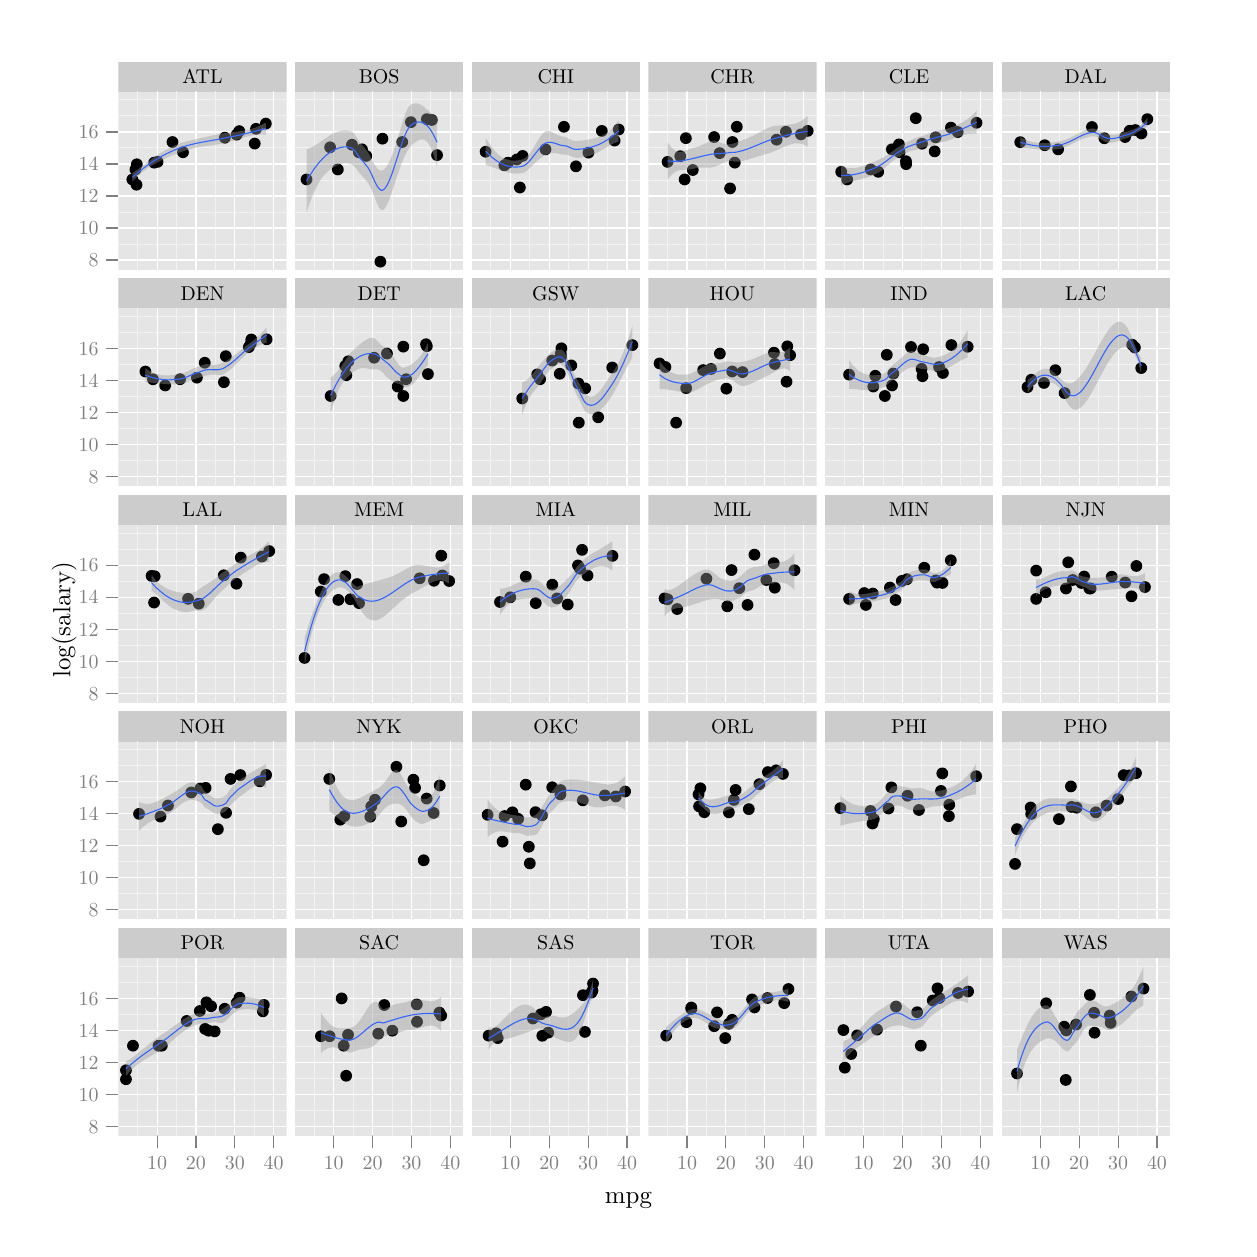
\begin{tikzpicture}[x=1pt,y=1pt]
\draw[color=white,opacity=0] (0,0) rectangle (433.62,433.62);
\begin{scope}
\path[clip] (  0.00,  0.00) rectangle (433.62,433.62);
\definecolor[named]{drawColor}{rgb}{0.06,0.82,0.87}
\end{scope}
\begin{scope}
\path[clip] (  0.00,  0.00) rectangle (433.62,433.62);
\definecolor[named]{drawColor}{rgb}{0.06,0.82,0.87}
\end{scope}
\begin{scope}
\path[clip] (  0.00,  0.00) rectangle (433.62,433.62);
\definecolor[named]{drawColor}{rgb}{0.06,0.82,0.87}
\end{scope}
\begin{scope}
\path[clip] (  0.00,  0.00) rectangle (433.62,433.62);
\definecolor[named]{drawColor}{rgb}{0.06,0.82,0.87}
\end{scope}
\begin{scope}
\path[clip] (  0.00,  0.00) rectangle (433.62,433.62);
\definecolor[named]{drawColor}{rgb}{0.06,0.82,0.87}
\end{scope}
\begin{scope}
\path[clip] (  0.00,  0.00) rectangle (433.62,433.62);
\definecolor[named]{drawColor}{rgb}{0.06,0.82,0.87}
\end{scope}
\begin{scope}
\path[clip] (  0.00,  0.00) rectangle (433.62,433.62);
\definecolor[named]{drawColor}{rgb}{0.06,0.82,0.87}
\end{scope}
\begin{scope}
\path[clip] (  0.00,  0.00) rectangle (433.62,433.62);
\definecolor[named]{drawColor}{rgb}{0.06,0.82,0.87}
\end{scope}
\begin{scope}
\path[clip] (  0.00,  0.00) rectangle (433.62,433.62);
\definecolor[named]{drawColor}{rgb}{0.06,0.82,0.87}
\end{scope}
\begin{scope}
\path[clip] (  0.00,  0.00) rectangle (433.62,433.62);
\definecolor[named]{drawColor}{rgb}{0.06,0.82,0.87}
\end{scope}
\begin{scope}
\path[clip] (  0.00,  0.00) rectangle (433.62,433.62);
\definecolor[named]{drawColor}{rgb}{0.06,0.82,0.87}
\end{scope}
\begin{scope}
\path[clip] (  0.00,  0.00) rectangle (433.62,433.62);
\definecolor[named]{drawColor}{rgb}{0.06,0.82,0.87}
\end{scope}
\begin{scope}
\path[clip] (  0.00,  0.00) rectangle (433.62,433.62);
\definecolor[named]{drawColor}{rgb}{0.06,0.82,0.87}
\end{scope}
\begin{scope}
\path[clip] (  0.00,  0.00) rectangle (433.62,433.62);
\definecolor[named]{drawColor}{rgb}{0.06,0.82,0.87}
\end{scope}
\begin{scope}
\path[clip] (  0.00,  0.00) rectangle (433.62,433.62);
\definecolor[named]{drawColor}{rgb}{0.06,0.82,0.87}
\end{scope}
\begin{scope}
\path[clip] (  0.00,  0.00) rectangle (433.62,433.62);
\definecolor[named]{drawColor}{rgb}{0.06,0.82,0.87}
\end{scope}
\begin{scope}
\path[clip] (  0.00,  0.00) rectangle (433.62,433.62);
\definecolor[named]{drawColor}{rgb}{0.06,0.82,0.87}
\end{scope}
\begin{scope}
\path[clip] (  0.00,  0.00) rectangle (433.62,433.62);
\definecolor[named]{drawColor}{rgb}{0.06,0.82,0.87}
\end{scope}
\begin{scope}
\path[clip] (  0.00,  0.00) rectangle (433.62,433.62);
\definecolor[named]{drawColor}{rgb}{0.06,0.82,0.87}
\end{scope}
\begin{scope}
\path[clip] (  0.00,  0.00) rectangle (433.62,433.62);
\definecolor[named]{drawColor}{rgb}{0.06,0.82,0.87}
\end{scope}
\begin{scope}
\path[clip] (  0.00,  0.00) rectangle (433.62,433.62);
\definecolor[named]{drawColor}{rgb}{0.06,0.82,0.87}
\end{scope}
\begin{scope}
\path[clip] (  0.00,  0.00) rectangle (433.62,433.62);
\definecolor[named]{drawColor}{rgb}{0.06,0.82,0.87}
\end{scope}
\begin{scope}
\path[clip] (  0.00,  0.00) rectangle (433.62,433.62);
\definecolor[named]{drawColor}{rgb}{0.06,0.82,0.87}
\end{scope}
\begin{scope}
\path[clip] (  0.00,  0.00) rectangle (433.62,433.62);
\definecolor[named]{drawColor}{rgb}{0.06,0.82,0.87}
\end{scope}
\begin{scope}
\path[clip] (  0.00,  0.00) rectangle (433.62,433.62);
\definecolor[named]{drawColor}{rgb}{0.06,0.82,0.87}
\end{scope}
\begin{scope}
\path[clip] (  0.00,  0.00) rectangle (433.62,433.62);
\definecolor[named]{drawColor}{rgb}{0.06,0.82,0.87}
\end{scope}
\begin{scope}
\path[clip] (  0.00,  0.00) rectangle (433.62,433.62);
\definecolor[named]{drawColor}{rgb}{0.06,0.82,0.87}
\end{scope}
\begin{scope}
\path[clip] (  0.00,  0.00) rectangle (433.62,433.62);
\definecolor[named]{drawColor}{rgb}{0.06,0.82,0.87}
\end{scope}
\begin{scope}
\path[clip] (  0.00,  0.00) rectangle (433.62,433.62);
\definecolor[named]{drawColor}{rgb}{0.06,0.82,0.87}
\end{scope}
\begin{scope}
\path[clip] (  0.00,  0.00) rectangle (433.62,433.62);
\definecolor[named]{drawColor}{rgb}{0.06,0.82,0.87}
\end{scope}
\begin{scope}
\path[clip] (  0.00,  0.00) rectangle (433.62,433.62);
\definecolor[named]{drawColor}{rgb}{0.06,0.82,0.87}
\end{scope}
\begin{scope}
\path[clip] (  0.00,  0.00) rectangle (433.62,433.62);
\definecolor[named]{drawColor}{rgb}{0.06,0.82,0.87}
\end{scope}
\begin{scope}
\path[clip] (  0.00,  0.00) rectangle (433.62,433.62);
\definecolor[named]{drawColor}{rgb}{0.06,0.82,0.87}
\end{scope}
\begin{scope}
\path[clip] (  0.00,  0.00) rectangle (433.62,433.62);
\definecolor[named]{drawColor}{rgb}{0.06,0.82,0.87}
\end{scope}
\begin{scope}
\path[clip] (  0.00,  0.00) rectangle (433.62,433.62);
\definecolor[named]{drawColor}{rgb}{0.06,0.82,0.87}
\end{scope}
\begin{scope}
\path[clip] (  0.00,  0.00) rectangle (433.62,433.62);
\definecolor[named]{drawColor}{rgb}{0.06,0.82,0.87}
\end{scope}
\begin{scope}
\path[clip] (  0.00,  0.00) rectangle (433.62,433.62);
\definecolor[named]{drawColor}{rgb}{0.06,0.82,0.87}
\end{scope}
\begin{scope}
\path[clip] (  0.00,  0.00) rectangle (433.62,433.62);
\definecolor[named]{drawColor}{rgb}{0.06,0.82,0.87}
\end{scope}
\begin{scope}
\path[clip] (  0.00,  0.00) rectangle (433.62,433.62);
\definecolor[named]{drawColor}{rgb}{0.06,0.82,0.87}
\end{scope}
\begin{scope}
\path[clip] (  0.00,  0.00) rectangle (433.62,433.62);
\definecolor[named]{drawColor}{rgb}{0.06,0.82,0.87}
\end{scope}
\begin{scope}
\path[clip] (  0.00,  0.00) rectangle (433.62,433.62);
\definecolor[named]{drawColor}{rgb}{0.06,0.82,0.87}
\end{scope}
\begin{scope}
\path[clip] (  0.00,  0.00) rectangle (433.62,433.62);
\definecolor[named]{drawColor}{rgb}{0.06,0.82,0.87}
\end{scope}
\begin{scope}
\path[clip] (  0.00,  0.00) rectangle (433.62,433.62);
\definecolor[named]{drawColor}{rgb}{0.06,0.82,0.87}
\end{scope}
\begin{scope}
\path[clip] (  0.00,  0.00) rectangle (433.62,433.62);
\definecolor[named]{drawColor}{rgb}{0.06,0.82,0.87}
\end{scope}
\begin{scope}
\path[clip] (  0.00,  0.00) rectangle (433.62,433.62);
\definecolor[named]{drawColor}{rgb}{0.06,0.82,0.87}
\end{scope}
\begin{scope}
\path[clip] (  0.00,  0.00) rectangle (433.62,433.62);
\definecolor[named]{drawColor}{rgb}{0.06,0.82,0.87}
\end{scope}
\begin{scope}
\path[clip] (  0.00,  0.00) rectangle (433.62,433.62);
\definecolor[named]{drawColor}{rgb}{0.06,0.82,0.87}
\end{scope}
\begin{scope}
\path[clip] (  0.00,  0.00) rectangle (433.62,433.62);
\definecolor[named]{drawColor}{rgb}{0.06,0.82,0.87}
\end{scope}
\begin{scope}
\path[clip] (  0.00,  0.00) rectangle (433.62,433.62);
\definecolor[named]{drawColor}{rgb}{0.06,0.82,0.87}
\end{scope}
\begin{scope}
\path[clip] (  0.00,  0.00) rectangle (433.62,433.62);
\definecolor[named]{drawColor}{rgb}{0.06,0.82,0.87}
\end{scope}
\begin{scope}
\path[clip] (  0.00,  0.00) rectangle (433.62,433.62);
\definecolor[named]{drawColor}{rgb}{0.06,0.82,0.87}
\end{scope}
\begin{scope}
\path[clip] (  0.00,  0.00) rectangle (433.62,433.62);
\definecolor[named]{drawColor}{rgb}{0.06,0.82,0.87}
\end{scope}
\begin{scope}
\path[clip] (  0.00,  0.00) rectangle (433.62,433.62);
\definecolor[named]{drawColor}{rgb}{0.06,0.82,0.87}
\end{scope}
\begin{scope}
\path[clip] (  0.00,  0.00) rectangle (433.62,433.62);
\definecolor[named]{drawColor}{rgb}{0.06,0.82,0.87}
\end{scope}
\begin{scope}
\path[clip] (  0.00,  0.00) rectangle (433.62,433.62);
\definecolor[named]{drawColor}{rgb}{0.06,0.82,0.87}
\end{scope}
\begin{scope}
\path[clip] (  0.00,  0.00) rectangle (433.62,433.62);
\definecolor[named]{drawColor}{rgb}{0.06,0.82,0.87}
\end{scope}
\begin{scope}
\path[clip] (  0.00,  0.00) rectangle (433.62,433.62);
\definecolor[named]{drawColor}{rgb}{0.06,0.82,0.87}
\end{scope}
\begin{scope}
\path[clip] (  0.00,  0.00) rectangle (433.62,433.62);
\definecolor[named]{drawColor}{rgb}{0.06,0.82,0.87}
\end{scope}
\begin{scope}
\path[clip] (  0.00,  0.00) rectangle (433.62,433.62);
\definecolor[named]{drawColor}{rgb}{0.06,0.82,0.87}
\end{scope}
\begin{scope}
\path[clip] (  0.00,  0.00) rectangle (433.62,433.62);
\definecolor[named]{drawColor}{rgb}{0.06,0.82,0.87}
\end{scope}
\begin{scope}
\path[clip] (  0.00,  0.00) rectangle (433.62,433.62);
\definecolor[named]{drawColor}{rgb}{0.06,0.82,0.87}
\end{scope}
\begin{scope}
\path[clip] (  0.00,  0.00) rectangle (433.62,433.62);
\definecolor[named]{drawColor}{rgb}{0.06,0.82,0.87}
\end{scope}
\begin{scope}
\path[clip] (  0.00,  0.00) rectangle (433.62,433.62);
\definecolor[named]{drawColor}{rgb}{0.06,0.82,0.87}
\end{scope}
\begin{scope}
\path[clip] (  0.00,  0.00) rectangle (433.62,433.62);
\definecolor[named]{drawColor}{rgb}{0.06,0.82,0.87}
\end{scope}
\begin{scope}
\path[clip] (  0.00,  0.00) rectangle (433.62,433.62);
\definecolor[named]{drawColor}{rgb}{0.06,0.82,0.87}
\end{scope}
\begin{scope}
\path[clip] (  0.00,  0.00) rectangle (433.62,433.62);
\definecolor[named]{drawColor}{rgb}{0.06,0.82,0.87}
\end{scope}
\begin{scope}
\path[clip] (  0.00,  0.00) rectangle (433.62,433.62);
\definecolor[named]{drawColor}{rgb}{0.06,0.82,0.87}
\definecolor[named]{fillColor}{rgb}{1.00,1.00,1.00}

\draw[fill=fillColor,draw opacity=0.00,] (  0.00,  0.00) rectangle (433.62,433.62);
\end{scope}
\begin{scope}
\path[clip] (  0.00,  0.00) rectangle (433.62,433.62);
\definecolor[named]{drawColor}{rgb}{0.06,0.82,0.87}
\end{scope}
\begin{scope}
\path[clip] (  0.00,  0.00) rectangle (433.62,433.62);
\definecolor[named]{drawColor}{rgb}{0.06,0.82,0.87}
\definecolor[named]{drawColor}{rgb}{0.00,0.00,0.00}

\node[color=drawColor,anchor=base,inner sep=0pt, outer sep=0pt, scale=  0.90] at (216.90,  9.03) {mpg%
};
\end{scope}
\begin{scope}
\path[clip] (  0.00,  0.00) rectangle (433.62,433.62);
\definecolor[named]{drawColor}{rgb}{0.06,0.82,0.87}
\definecolor[named]{drawColor}{rgb}{0.00,0.00,0.00}

\node[rotate= 90.00,color=drawColor,anchor=base,inner sep=0pt, outer sep=0pt, scale=  0.90] at ( 15.23,219.91) {log(salary)%
};
\end{scope}
\begin{scope}
\path[clip] (  0.00,  0.00) rectangle (433.62,433.62);
\definecolor[named]{drawColor}{rgb}{0.06,0.82,0.87}
\end{scope}
\begin{scope}
\path[clip] ( 18.24,410.59) rectangle ( 32.55,421.57);
\definecolor[named]{drawColor}{rgb}{0.06,0.82,0.87}
\end{scope}
\begin{scope}
\path[clip] (  0.00,  0.00) rectangle (433.62,433.62);
\definecolor[named]{drawColor}{rgb}{0.06,0.82,0.87}
\end{scope}
\begin{scope}
\path[clip] (  0.00,  0.00) rectangle (433.62,433.62);
\definecolor[named]{drawColor}{rgb}{0.06,0.82,0.87}
\end{scope}
\begin{scope}
\path[clip] (  0.00,  0.00) rectangle (433.62,433.62);
\definecolor[named]{drawColor}{rgb}{0.06,0.82,0.87}
\end{scope}
\begin{scope}
\path[clip] ( 18.24,346.33) rectangle ( 32.55,346.33);
\definecolor[named]{drawColor}{rgb}{0.06,0.82,0.87}
\end{scope}
\begin{scope}
\path[clip] (  0.00,  0.00) rectangle (433.62,433.62);
\definecolor[named]{drawColor}{rgb}{0.06,0.82,0.87}
\end{scope}
\begin{scope}
\path[clip] ( 18.24,343.32) rectangle ( 32.55,346.33);
\definecolor[named]{drawColor}{rgb}{0.06,0.82,0.87}
\end{scope}
\begin{scope}
\path[clip] (  0.00,  0.00) rectangle (433.62,433.62);
\definecolor[named]{drawColor}{rgb}{0.06,0.82,0.87}
\end{scope}
\begin{scope}
\path[clip] ( 18.24,332.34) rectangle ( 32.55,343.32);
\definecolor[named]{drawColor}{rgb}{0.06,0.82,0.87}
\end{scope}
\begin{scope}
\path[clip] (  0.00,  0.00) rectangle (433.62,433.62);
\definecolor[named]{drawColor}{rgb}{0.06,0.82,0.87}
\end{scope}
\begin{scope}
\path[clip] (  0.00,  0.00) rectangle (433.62,433.62);
\definecolor[named]{drawColor}{rgb}{0.06,0.82,0.87}
\end{scope}
\begin{scope}
\path[clip] (  0.00,  0.00) rectangle (433.62,433.62);
\definecolor[named]{drawColor}{rgb}{0.06,0.82,0.87}
\end{scope}
\begin{scope}
\path[clip] ( 18.24,268.08) rectangle ( 32.55,268.08);
\definecolor[named]{drawColor}{rgb}{0.06,0.82,0.87}
\end{scope}
\begin{scope}
\path[clip] (  0.00,  0.00) rectangle (433.62,433.62);
\definecolor[named]{drawColor}{rgb}{0.06,0.82,0.87}
\end{scope}
\begin{scope}
\path[clip] ( 18.24,265.07) rectangle ( 32.55,268.08);
\definecolor[named]{drawColor}{rgb}{0.06,0.82,0.87}
\end{scope}
\begin{scope}
\path[clip] (  0.00,  0.00) rectangle (433.62,433.62);
\definecolor[named]{drawColor}{rgb}{0.06,0.82,0.87}
\end{scope}
\begin{scope}
\path[clip] ( 18.24,254.09) rectangle ( 32.55,265.07);
\definecolor[named]{drawColor}{rgb}{0.06,0.82,0.87}
\end{scope}
\begin{scope}
\path[clip] (  0.00,  0.00) rectangle (433.62,433.62);
\definecolor[named]{drawColor}{rgb}{0.06,0.82,0.87}
\end{scope}
\begin{scope}
\path[clip] (  0.00,  0.00) rectangle (433.62,433.62);
\definecolor[named]{drawColor}{rgb}{0.06,0.82,0.87}
\end{scope}
\begin{scope}
\path[clip] (  0.00,  0.00) rectangle (433.62,433.62);
\definecolor[named]{drawColor}{rgb}{0.06,0.82,0.87}
\end{scope}
\begin{scope}
\path[clip] ( 18.24,189.83) rectangle ( 32.55,189.83);
\definecolor[named]{drawColor}{rgb}{0.06,0.82,0.87}
\end{scope}
\begin{scope}
\path[clip] (  0.00,  0.00) rectangle (433.62,433.62);
\definecolor[named]{drawColor}{rgb}{0.06,0.82,0.87}
\end{scope}
\begin{scope}
\path[clip] ( 18.24,186.82) rectangle ( 32.55,189.83);
\definecolor[named]{drawColor}{rgb}{0.06,0.82,0.87}
\end{scope}
\begin{scope}
\path[clip] (  0.00,  0.00) rectangle (433.62,433.62);
\definecolor[named]{drawColor}{rgb}{0.06,0.82,0.87}
\end{scope}
\begin{scope}
\path[clip] ( 18.24,175.84) rectangle ( 32.55,186.82);
\definecolor[named]{drawColor}{rgb}{0.06,0.82,0.87}
\end{scope}
\begin{scope}
\path[clip] (  0.00,  0.00) rectangle (433.62,433.62);
\definecolor[named]{drawColor}{rgb}{0.06,0.82,0.87}
\end{scope}
\begin{scope}
\path[clip] (  0.00,  0.00) rectangle (433.62,433.62);
\definecolor[named]{drawColor}{rgb}{0.06,0.82,0.87}
\end{scope}
\begin{scope}
\path[clip] (  0.00,  0.00) rectangle (433.62,433.62);
\definecolor[named]{drawColor}{rgb}{0.06,0.82,0.87}
\end{scope}
\begin{scope}
\path[clip] ( 18.24,111.58) rectangle ( 32.55,111.58);
\definecolor[named]{drawColor}{rgb}{0.06,0.82,0.87}
\end{scope}
\begin{scope}
\path[clip] (  0.00,  0.00) rectangle (433.62,433.62);
\definecolor[named]{drawColor}{rgb}{0.06,0.82,0.87}
\end{scope}
\begin{scope}
\path[clip] ( 18.24,108.57) rectangle ( 32.55,111.58);
\definecolor[named]{drawColor}{rgb}{0.06,0.82,0.87}
\end{scope}
\begin{scope}
\path[clip] (  0.00,  0.00) rectangle (433.62,433.62);
\definecolor[named]{drawColor}{rgb}{0.06,0.82,0.87}
\end{scope}
\begin{scope}
\path[clip] ( 18.24, 97.59) rectangle ( 32.55,108.57);
\definecolor[named]{drawColor}{rgb}{0.06,0.82,0.87}
\end{scope}
\begin{scope}
\path[clip] (  0.00,  0.00) rectangle (433.62,433.62);
\definecolor[named]{drawColor}{rgb}{0.06,0.82,0.87}
\end{scope}
\begin{scope}
\path[clip] (  0.00,  0.00) rectangle (433.62,433.62);
\definecolor[named]{drawColor}{rgb}{0.06,0.82,0.87}
\end{scope}
\begin{scope}
\path[clip] (  0.00,  0.00) rectangle (433.62,433.62);
\definecolor[named]{drawColor}{rgb}{0.06,0.82,0.87}
\end{scope}
\begin{scope}
\path[clip] ( 18.24, 21.25) rectangle ( 32.55, 33.33);
\definecolor[named]{drawColor}{rgb}{0.06,0.82,0.87}
\end{scope}
\begin{scope}
\path[clip] (  0.00,  0.00) rectangle (433.62,433.62);
\definecolor[named]{drawColor}{rgb}{0.06,0.82,0.87}
\end{scope}
\begin{scope}
\path[clip] ( 18.24, 18.24) rectangle ( 32.55, 21.25);
\definecolor[named]{drawColor}{rgb}{0.06,0.82,0.87}
\end{scope}
\begin{scope}
\path[clip] (  0.00,  0.00) rectangle (433.62,433.62);
\definecolor[named]{drawColor}{rgb}{0.06,0.82,0.87}
\end{scope}
\begin{scope}
\path[clip] ( 32.55,410.59) rectangle ( 93.38,421.57);
\definecolor[named]{drawColor}{rgb}{0.06,0.82,0.87}
\end{scope}
\begin{scope}
\path[clip] (  0.00,  0.00) rectangle (433.62,433.62);
\definecolor[named]{drawColor}{rgb}{0.06,0.82,0.87}
\end{scope}
\begin{scope}
\path[clip] ( 32.55,346.33) rectangle ( 93.38,410.59);
\definecolor[named]{drawColor}{rgb}{0.06,0.82,0.87}
\end{scope}
\begin{scope}
\path[clip] (  0.00,  0.00) rectangle (433.62,433.62);
\definecolor[named]{drawColor}{rgb}{0.06,0.82,0.87}
\end{scope}
\begin{scope}
\path[clip] ( 32.55,346.33) rectangle ( 93.38,346.33);
\definecolor[named]{drawColor}{rgb}{0.06,0.82,0.87}
\end{scope}
\begin{scope}
\path[clip] (  0.00,  0.00) rectangle (433.62,433.62);
\definecolor[named]{drawColor}{rgb}{0.06,0.82,0.87}
\end{scope}
\begin{scope}
\path[clip] ( 32.55,343.32) rectangle ( 93.38,346.33);
\definecolor[named]{drawColor}{rgb}{0.06,0.82,0.87}
\end{scope}
\begin{scope}
\path[clip] (  0.00,  0.00) rectangle (433.62,433.62);
\definecolor[named]{drawColor}{rgb}{0.06,0.82,0.87}
\end{scope}
\begin{scope}
\path[clip] ( 32.55,332.34) rectangle ( 93.38,343.32);
\definecolor[named]{drawColor}{rgb}{0.06,0.82,0.87}
\end{scope}
\begin{scope}
\path[clip] (  0.00,  0.00) rectangle (433.62,433.62);
\definecolor[named]{drawColor}{rgb}{0.06,0.82,0.87}
\end{scope}
\begin{scope}
\path[clip] ( 32.55,268.08) rectangle ( 93.38,332.34);
\definecolor[named]{drawColor}{rgb}{0.06,0.82,0.87}
\end{scope}
\begin{scope}
\path[clip] (  0.00,  0.00) rectangle (433.62,433.62);
\definecolor[named]{drawColor}{rgb}{0.06,0.82,0.87}
\end{scope}
\begin{scope}
\path[clip] ( 32.55,268.08) rectangle ( 93.38,268.08);
\definecolor[named]{drawColor}{rgb}{0.06,0.82,0.87}
\end{scope}
\begin{scope}
\path[clip] (  0.00,  0.00) rectangle (433.62,433.62);
\definecolor[named]{drawColor}{rgb}{0.06,0.82,0.87}
\end{scope}
\begin{scope}
\path[clip] ( 32.55,265.07) rectangle ( 93.38,268.08);
\definecolor[named]{drawColor}{rgb}{0.06,0.82,0.87}
\end{scope}
\begin{scope}
\path[clip] (  0.00,  0.00) rectangle (433.62,433.62);
\definecolor[named]{drawColor}{rgb}{0.06,0.82,0.87}
\end{scope}
\begin{scope}
\path[clip] ( 32.55,254.09) rectangle ( 93.38,265.07);
\definecolor[named]{drawColor}{rgb}{0.06,0.82,0.87}
\end{scope}
\begin{scope}
\path[clip] (  0.00,  0.00) rectangle (433.62,433.62);
\definecolor[named]{drawColor}{rgb}{0.06,0.82,0.87}
\end{scope}
\begin{scope}
\path[clip] ( 32.55,189.83) rectangle ( 93.38,254.09);
\definecolor[named]{drawColor}{rgb}{0.06,0.82,0.87}
\end{scope}
\begin{scope}
\path[clip] (  0.00,  0.00) rectangle (433.62,433.62);
\definecolor[named]{drawColor}{rgb}{0.06,0.82,0.87}
\end{scope}
\begin{scope}
\path[clip] ( 32.55,189.83) rectangle ( 93.38,189.83);
\definecolor[named]{drawColor}{rgb}{0.06,0.82,0.87}
\end{scope}
\begin{scope}
\path[clip] (  0.00,  0.00) rectangle (433.62,433.62);
\definecolor[named]{drawColor}{rgb}{0.06,0.82,0.87}
\end{scope}
\begin{scope}
\path[clip] ( 32.55,186.82) rectangle ( 93.38,189.83);
\definecolor[named]{drawColor}{rgb}{0.06,0.82,0.87}
\end{scope}
\begin{scope}
\path[clip] (  0.00,  0.00) rectangle (433.62,433.62);
\definecolor[named]{drawColor}{rgb}{0.06,0.82,0.87}
\end{scope}
\begin{scope}
\path[clip] ( 32.55,175.84) rectangle ( 93.38,186.82);
\definecolor[named]{drawColor}{rgb}{0.06,0.82,0.87}
\end{scope}
\begin{scope}
\path[clip] (  0.00,  0.00) rectangle (433.62,433.62);
\definecolor[named]{drawColor}{rgb}{0.06,0.82,0.87}
\end{scope}
\begin{scope}
\path[clip] ( 32.55,111.58) rectangle ( 93.38,175.84);
\definecolor[named]{drawColor}{rgb}{0.06,0.82,0.87}
\end{scope}
\begin{scope}
\path[clip] (  0.00,  0.00) rectangle (433.62,433.62);
\definecolor[named]{drawColor}{rgb}{0.06,0.82,0.87}
\end{scope}
\begin{scope}
\path[clip] ( 32.55,111.58) rectangle ( 93.38,111.58);
\definecolor[named]{drawColor}{rgb}{0.06,0.82,0.87}
\end{scope}
\begin{scope}
\path[clip] (  0.00,  0.00) rectangle (433.62,433.62);
\definecolor[named]{drawColor}{rgb}{0.06,0.82,0.87}
\end{scope}
\begin{scope}
\path[clip] ( 32.55,108.57) rectangle ( 93.38,111.58);
\definecolor[named]{drawColor}{rgb}{0.06,0.82,0.87}
\end{scope}
\begin{scope}
\path[clip] (  0.00,  0.00) rectangle (433.62,433.62);
\definecolor[named]{drawColor}{rgb}{0.06,0.82,0.87}
\end{scope}
\begin{scope}
\path[clip] ( 32.55, 97.59) rectangle ( 93.38,108.57);
\definecolor[named]{drawColor}{rgb}{0.06,0.82,0.87}
\end{scope}
\begin{scope}
\path[clip] (  0.00,  0.00) rectangle (433.62,433.62);
\definecolor[named]{drawColor}{rgb}{0.06,0.82,0.87}
\end{scope}
\begin{scope}
\path[clip] ( 32.55, 33.33) rectangle ( 93.38, 97.59);
\definecolor[named]{drawColor}{rgb}{0.06,0.82,0.87}
\end{scope}
\begin{scope}
\path[clip] (  0.00,  0.00) rectangle (433.62,433.62);
\definecolor[named]{drawColor}{rgb}{0.06,0.82,0.87}
\end{scope}
\begin{scope}
\path[clip] (  0.00,  0.00) rectangle (433.62,433.62);
\definecolor[named]{drawColor}{rgb}{0.06,0.82,0.87}
\end{scope}
\begin{scope}
\path[clip] (  0.00,  0.00) rectangle (433.62,433.62);
\definecolor[named]{drawColor}{rgb}{0.06,0.82,0.87}
\end{scope}
\begin{scope}
\path[clip] ( 32.55, 18.24) rectangle ( 93.38, 21.25);
\definecolor[named]{drawColor}{rgb}{0.06,0.82,0.87}
\end{scope}
\begin{scope}
\path[clip] (  0.00,  0.00) rectangle (433.62,433.62);
\definecolor[named]{drawColor}{rgb}{0.06,0.82,0.87}
\end{scope}
\begin{scope}
\path[clip] ( 93.38,410.59) rectangle ( 96.39,421.57);
\definecolor[named]{drawColor}{rgb}{0.06,0.82,0.87}
\end{scope}
\begin{scope}
\path[clip] (  0.00,  0.00) rectangle (433.62,433.62);
\definecolor[named]{drawColor}{rgb}{0.06,0.82,0.87}
\end{scope}
\begin{scope}
\path[clip] ( 93.38,346.33) rectangle ( 96.39,410.59);
\definecolor[named]{drawColor}{rgb}{0.06,0.82,0.87}
\end{scope}
\begin{scope}
\path[clip] (  0.00,  0.00) rectangle (433.62,433.62);
\definecolor[named]{drawColor}{rgb}{0.06,0.82,0.87}
\end{scope}
\begin{scope}
\path[clip] ( 93.38,346.33) rectangle ( 96.39,346.33);
\definecolor[named]{drawColor}{rgb}{0.06,0.82,0.87}
\end{scope}
\begin{scope}
\path[clip] (  0.00,  0.00) rectangle (433.62,433.62);
\definecolor[named]{drawColor}{rgb}{0.06,0.82,0.87}
\end{scope}
\begin{scope}
\path[clip] ( 93.38,343.32) rectangle ( 96.39,346.33);
\definecolor[named]{drawColor}{rgb}{0.06,0.82,0.87}
\end{scope}
\begin{scope}
\path[clip] (  0.00,  0.00) rectangle (433.62,433.62);
\definecolor[named]{drawColor}{rgb}{0.06,0.82,0.87}
\end{scope}
\begin{scope}
\path[clip] ( 93.38,332.34) rectangle ( 96.39,343.32);
\definecolor[named]{drawColor}{rgb}{0.06,0.82,0.87}
\end{scope}
\begin{scope}
\path[clip] (  0.00,  0.00) rectangle (433.62,433.62);
\definecolor[named]{drawColor}{rgb}{0.06,0.82,0.87}
\end{scope}
\begin{scope}
\path[clip] ( 93.38,268.08) rectangle ( 96.39,332.34);
\definecolor[named]{drawColor}{rgb}{0.06,0.82,0.87}
\end{scope}
\begin{scope}
\path[clip] (  0.00,  0.00) rectangle (433.62,433.62);
\definecolor[named]{drawColor}{rgb}{0.06,0.82,0.87}
\end{scope}
\begin{scope}
\path[clip] ( 93.38,268.08) rectangle ( 96.39,268.08);
\definecolor[named]{drawColor}{rgb}{0.06,0.82,0.87}
\end{scope}
\begin{scope}
\path[clip] (  0.00,  0.00) rectangle (433.62,433.62);
\definecolor[named]{drawColor}{rgb}{0.06,0.82,0.87}
\end{scope}
\begin{scope}
\path[clip] ( 93.38,265.07) rectangle ( 96.39,268.08);
\definecolor[named]{drawColor}{rgb}{0.06,0.82,0.87}
\end{scope}
\begin{scope}
\path[clip] (  0.00,  0.00) rectangle (433.62,433.62);
\definecolor[named]{drawColor}{rgb}{0.06,0.82,0.87}
\end{scope}
\begin{scope}
\path[clip] ( 93.38,254.09) rectangle ( 96.39,265.07);
\definecolor[named]{drawColor}{rgb}{0.06,0.82,0.87}
\end{scope}
\begin{scope}
\path[clip] (  0.00,  0.00) rectangle (433.62,433.62);
\definecolor[named]{drawColor}{rgb}{0.06,0.82,0.87}
\end{scope}
\begin{scope}
\path[clip] ( 93.38,189.83) rectangle ( 96.39,254.09);
\definecolor[named]{drawColor}{rgb}{0.06,0.82,0.87}
\end{scope}
\begin{scope}
\path[clip] (  0.00,  0.00) rectangle (433.62,433.62);
\definecolor[named]{drawColor}{rgb}{0.06,0.82,0.87}
\end{scope}
\begin{scope}
\path[clip] ( 93.38,189.83) rectangle ( 96.39,189.83);
\definecolor[named]{drawColor}{rgb}{0.06,0.82,0.87}
\end{scope}
\begin{scope}
\path[clip] (  0.00,  0.00) rectangle (433.62,433.62);
\definecolor[named]{drawColor}{rgb}{0.06,0.82,0.87}
\end{scope}
\begin{scope}
\path[clip] ( 93.38,186.82) rectangle ( 96.39,189.83);
\definecolor[named]{drawColor}{rgb}{0.06,0.82,0.87}
\end{scope}
\begin{scope}
\path[clip] (  0.00,  0.00) rectangle (433.62,433.62);
\definecolor[named]{drawColor}{rgb}{0.06,0.82,0.87}
\end{scope}
\begin{scope}
\path[clip] ( 93.38,175.84) rectangle ( 96.39,186.82);
\definecolor[named]{drawColor}{rgb}{0.06,0.82,0.87}
\end{scope}
\begin{scope}
\path[clip] (  0.00,  0.00) rectangle (433.62,433.62);
\definecolor[named]{drawColor}{rgb}{0.06,0.82,0.87}
\end{scope}
\begin{scope}
\path[clip] ( 93.38,111.58) rectangle ( 96.39,175.84);
\definecolor[named]{drawColor}{rgb}{0.06,0.82,0.87}
\end{scope}
\begin{scope}
\path[clip] (  0.00,  0.00) rectangle (433.62,433.62);
\definecolor[named]{drawColor}{rgb}{0.06,0.82,0.87}
\end{scope}
\begin{scope}
\path[clip] ( 93.38,111.58) rectangle ( 96.39,111.58);
\definecolor[named]{drawColor}{rgb}{0.06,0.82,0.87}
\end{scope}
\begin{scope}
\path[clip] (  0.00,  0.00) rectangle (433.62,433.62);
\definecolor[named]{drawColor}{rgb}{0.06,0.82,0.87}
\end{scope}
\begin{scope}
\path[clip] ( 93.38,108.57) rectangle ( 96.39,111.58);
\definecolor[named]{drawColor}{rgb}{0.06,0.82,0.87}
\end{scope}
\begin{scope}
\path[clip] (  0.00,  0.00) rectangle (433.62,433.62);
\definecolor[named]{drawColor}{rgb}{0.06,0.82,0.87}
\end{scope}
\begin{scope}
\path[clip] ( 93.38, 97.59) rectangle ( 96.39,108.57);
\definecolor[named]{drawColor}{rgb}{0.06,0.82,0.87}
\end{scope}
\begin{scope}
\path[clip] (  0.00,  0.00) rectangle (433.62,433.62);
\definecolor[named]{drawColor}{rgb}{0.06,0.82,0.87}
\end{scope}
\begin{scope}
\path[clip] ( 93.38, 33.33) rectangle ( 96.39, 97.59);
\definecolor[named]{drawColor}{rgb}{0.06,0.82,0.87}
\end{scope}
\begin{scope}
\path[clip] (  0.00,  0.00) rectangle (433.62,433.62);
\definecolor[named]{drawColor}{rgb}{0.06,0.82,0.87}
\end{scope}
\begin{scope}
\path[clip] ( 93.38, 21.25) rectangle ( 96.39, 33.33);
\definecolor[named]{drawColor}{rgb}{0.06,0.82,0.87}
\end{scope}
\begin{scope}
\path[clip] (  0.00,  0.00) rectangle (433.62,433.62);
\definecolor[named]{drawColor}{rgb}{0.06,0.82,0.87}
\end{scope}
\begin{scope}
\path[clip] ( 93.38, 18.24) rectangle ( 96.39, 21.25);
\definecolor[named]{drawColor}{rgb}{0.06,0.82,0.87}
\end{scope}
\begin{scope}
\path[clip] (  0.00,  0.00) rectangle (433.62,433.62);
\definecolor[named]{drawColor}{rgb}{0.06,0.82,0.87}
\end{scope}
\begin{scope}
\path[clip] ( 96.39,410.59) rectangle ( 96.39,421.57);
\definecolor[named]{drawColor}{rgb}{0.06,0.82,0.87}
\end{scope}
\begin{scope}
\path[clip] (  0.00,  0.00) rectangle (433.62,433.62);
\definecolor[named]{drawColor}{rgb}{0.06,0.82,0.87}
\end{scope}
\begin{scope}
\path[clip] ( 96.39,346.33) rectangle ( 96.39,410.59);
\definecolor[named]{drawColor}{rgb}{0.06,0.82,0.87}
\end{scope}
\begin{scope}
\path[clip] (  0.00,  0.00) rectangle (433.62,433.62);
\definecolor[named]{drawColor}{rgb}{0.06,0.82,0.87}
\end{scope}
\begin{scope}
\path[clip] ( 96.39,346.33) rectangle ( 96.39,346.33);
\definecolor[named]{drawColor}{rgb}{0.06,0.82,0.87}
\end{scope}
\begin{scope}
\path[clip] (  0.00,  0.00) rectangle (433.62,433.62);
\definecolor[named]{drawColor}{rgb}{0.06,0.82,0.87}
\end{scope}
\begin{scope}
\path[clip] ( 96.39,343.32) rectangle ( 96.39,346.33);
\definecolor[named]{drawColor}{rgb}{0.06,0.82,0.87}
\end{scope}
\begin{scope}
\path[clip] (  0.00,  0.00) rectangle (433.62,433.62);
\definecolor[named]{drawColor}{rgb}{0.06,0.82,0.87}
\end{scope}
\begin{scope}
\path[clip] ( 96.39,332.34) rectangle ( 96.39,343.32);
\definecolor[named]{drawColor}{rgb}{0.06,0.82,0.87}
\end{scope}
\begin{scope}
\path[clip] (  0.00,  0.00) rectangle (433.62,433.62);
\definecolor[named]{drawColor}{rgb}{0.06,0.82,0.87}
\end{scope}
\begin{scope}
\path[clip] ( 96.39,268.08) rectangle ( 96.39,332.34);
\definecolor[named]{drawColor}{rgb}{0.06,0.82,0.87}
\end{scope}
\begin{scope}
\path[clip] (  0.00,  0.00) rectangle (433.62,433.62);
\definecolor[named]{drawColor}{rgb}{0.06,0.82,0.87}
\end{scope}
\begin{scope}
\path[clip] ( 96.39,268.08) rectangle ( 96.39,268.08);
\definecolor[named]{drawColor}{rgb}{0.06,0.82,0.87}
\end{scope}
\begin{scope}
\path[clip] (  0.00,  0.00) rectangle (433.62,433.62);
\definecolor[named]{drawColor}{rgb}{0.06,0.82,0.87}
\end{scope}
\begin{scope}
\path[clip] ( 96.39,265.07) rectangle ( 96.39,268.08);
\definecolor[named]{drawColor}{rgb}{0.06,0.82,0.87}
\end{scope}
\begin{scope}
\path[clip] (  0.00,  0.00) rectangle (433.62,433.62);
\definecolor[named]{drawColor}{rgb}{0.06,0.82,0.87}
\end{scope}
\begin{scope}
\path[clip] ( 96.39,254.09) rectangle ( 96.39,265.07);
\definecolor[named]{drawColor}{rgb}{0.06,0.82,0.87}
\end{scope}
\begin{scope}
\path[clip] (  0.00,  0.00) rectangle (433.62,433.62);
\definecolor[named]{drawColor}{rgb}{0.06,0.82,0.87}
\end{scope}
\begin{scope}
\path[clip] ( 96.39,189.83) rectangle ( 96.39,254.09);
\definecolor[named]{drawColor}{rgb}{0.06,0.82,0.87}
\end{scope}
\begin{scope}
\path[clip] (  0.00,  0.00) rectangle (433.62,433.62);
\definecolor[named]{drawColor}{rgb}{0.06,0.82,0.87}
\end{scope}
\begin{scope}
\path[clip] ( 96.39,189.83) rectangle ( 96.39,189.83);
\definecolor[named]{drawColor}{rgb}{0.06,0.82,0.87}
\end{scope}
\begin{scope}
\path[clip] (  0.00,  0.00) rectangle (433.62,433.62);
\definecolor[named]{drawColor}{rgb}{0.06,0.82,0.87}
\end{scope}
\begin{scope}
\path[clip] ( 96.39,186.82) rectangle ( 96.39,189.83);
\definecolor[named]{drawColor}{rgb}{0.06,0.82,0.87}
\end{scope}
\begin{scope}
\path[clip] (  0.00,  0.00) rectangle (433.62,433.62);
\definecolor[named]{drawColor}{rgb}{0.06,0.82,0.87}
\end{scope}
\begin{scope}
\path[clip] ( 96.39,175.84) rectangle ( 96.39,186.82);
\definecolor[named]{drawColor}{rgb}{0.06,0.82,0.87}
\end{scope}
\begin{scope}
\path[clip] (  0.00,  0.00) rectangle (433.62,433.62);
\definecolor[named]{drawColor}{rgb}{0.06,0.82,0.87}
\end{scope}
\begin{scope}
\path[clip] ( 96.39,111.58) rectangle ( 96.39,175.84);
\definecolor[named]{drawColor}{rgb}{0.06,0.82,0.87}
\end{scope}
\begin{scope}
\path[clip] (  0.00,  0.00) rectangle (433.62,433.62);
\definecolor[named]{drawColor}{rgb}{0.06,0.82,0.87}
\end{scope}
\begin{scope}
\path[clip] ( 96.39,111.58) rectangle ( 96.39,111.58);
\definecolor[named]{drawColor}{rgb}{0.06,0.82,0.87}
\end{scope}
\begin{scope}
\path[clip] (  0.00,  0.00) rectangle (433.62,433.62);
\definecolor[named]{drawColor}{rgb}{0.06,0.82,0.87}
\end{scope}
\begin{scope}
\path[clip] ( 96.39,108.57) rectangle ( 96.39,111.58);
\definecolor[named]{drawColor}{rgb}{0.06,0.82,0.87}
\end{scope}
\begin{scope}
\path[clip] (  0.00,  0.00) rectangle (433.62,433.62);
\definecolor[named]{drawColor}{rgb}{0.06,0.82,0.87}
\end{scope}
\begin{scope}
\path[clip] ( 96.39, 97.59) rectangle ( 96.39,108.57);
\definecolor[named]{drawColor}{rgb}{0.06,0.82,0.87}
\end{scope}
\begin{scope}
\path[clip] (  0.00,  0.00) rectangle (433.62,433.62);
\definecolor[named]{drawColor}{rgb}{0.06,0.82,0.87}
\end{scope}
\begin{scope}
\path[clip] ( 96.39, 33.33) rectangle ( 96.39, 97.59);
\definecolor[named]{drawColor}{rgb}{0.06,0.82,0.87}
\end{scope}
\begin{scope}
\path[clip] (  0.00,  0.00) rectangle (433.62,433.62);
\definecolor[named]{drawColor}{rgb}{0.06,0.82,0.87}
\end{scope}
\begin{scope}
\path[clip] ( 96.39, 21.25) rectangle ( 96.39, 33.33);
\definecolor[named]{drawColor}{rgb}{0.06,0.82,0.87}
\end{scope}
\begin{scope}
\path[clip] (  0.00,  0.00) rectangle (433.62,433.62);
\definecolor[named]{drawColor}{rgb}{0.06,0.82,0.87}
\end{scope}
\begin{scope}
\path[clip] ( 96.39, 18.24) rectangle ( 96.39, 21.25);
\definecolor[named]{drawColor}{rgb}{0.06,0.82,0.87}
\end{scope}
\begin{scope}
\path[clip] (  0.00,  0.00) rectangle (433.62,433.62);
\definecolor[named]{drawColor}{rgb}{0.06,0.82,0.87}
\end{scope}
\begin{scope}
\path[clip] ( 96.39,410.59) rectangle (157.21,421.57);
\definecolor[named]{drawColor}{rgb}{0.06,0.82,0.87}
\end{scope}
\begin{scope}
\path[clip] (  0.00,  0.00) rectangle (433.62,433.62);
\definecolor[named]{drawColor}{rgb}{0.06,0.82,0.87}
\end{scope}
\begin{scope}
\path[clip] ( 96.39,346.33) rectangle (157.21,410.59);
\definecolor[named]{drawColor}{rgb}{0.06,0.82,0.87}
\end{scope}
\begin{scope}
\path[clip] (  0.00,  0.00) rectangle (433.62,433.62);
\definecolor[named]{drawColor}{rgb}{0.06,0.82,0.87}
\end{scope}
\begin{scope}
\path[clip] ( 96.39,346.33) rectangle (157.21,346.33);
\definecolor[named]{drawColor}{rgb}{0.06,0.82,0.87}
\end{scope}
\begin{scope}
\path[clip] (  0.00,  0.00) rectangle (433.62,433.62);
\definecolor[named]{drawColor}{rgb}{0.06,0.82,0.87}
\end{scope}
\begin{scope}
\path[clip] ( 96.39,343.32) rectangle (157.21,346.33);
\definecolor[named]{drawColor}{rgb}{0.06,0.82,0.87}
\end{scope}
\begin{scope}
\path[clip] (  0.00,  0.00) rectangle (433.62,433.62);
\definecolor[named]{drawColor}{rgb}{0.06,0.82,0.87}
\end{scope}
\begin{scope}
\path[clip] ( 96.39,332.34) rectangle (157.21,343.32);
\definecolor[named]{drawColor}{rgb}{0.06,0.82,0.87}
\end{scope}
\begin{scope}
\path[clip] (  0.00,  0.00) rectangle (433.62,433.62);
\definecolor[named]{drawColor}{rgb}{0.06,0.82,0.87}
\end{scope}
\begin{scope}
\path[clip] ( 96.39,268.08) rectangle (157.21,332.34);
\definecolor[named]{drawColor}{rgb}{0.06,0.82,0.87}
\end{scope}
\begin{scope}
\path[clip] (  0.00,  0.00) rectangle (433.62,433.62);
\definecolor[named]{drawColor}{rgb}{0.06,0.82,0.87}
\end{scope}
\begin{scope}
\path[clip] ( 96.39,268.08) rectangle (157.21,268.08);
\definecolor[named]{drawColor}{rgb}{0.06,0.82,0.87}
\end{scope}
\begin{scope}
\path[clip] (  0.00,  0.00) rectangle (433.62,433.62);
\definecolor[named]{drawColor}{rgb}{0.06,0.82,0.87}
\end{scope}
\begin{scope}
\path[clip] ( 96.39,265.07) rectangle (157.21,268.08);
\definecolor[named]{drawColor}{rgb}{0.06,0.82,0.87}
\end{scope}
\begin{scope}
\path[clip] (  0.00,  0.00) rectangle (433.62,433.62);
\definecolor[named]{drawColor}{rgb}{0.06,0.82,0.87}
\end{scope}
\begin{scope}
\path[clip] ( 96.39,254.09) rectangle (157.21,265.07);
\definecolor[named]{drawColor}{rgb}{0.06,0.82,0.87}
\end{scope}
\begin{scope}
\path[clip] (  0.00,  0.00) rectangle (433.62,433.62);
\definecolor[named]{drawColor}{rgb}{0.06,0.82,0.87}
\end{scope}
\begin{scope}
\path[clip] ( 96.39,189.83) rectangle (157.21,254.09);
\definecolor[named]{drawColor}{rgb}{0.06,0.82,0.87}
\end{scope}
\begin{scope}
\path[clip] (  0.00,  0.00) rectangle (433.62,433.62);
\definecolor[named]{drawColor}{rgb}{0.06,0.82,0.87}
\end{scope}
\begin{scope}
\path[clip] ( 96.39,189.83) rectangle (157.21,189.83);
\definecolor[named]{drawColor}{rgb}{0.06,0.82,0.87}
\end{scope}
\begin{scope}
\path[clip] (  0.00,  0.00) rectangle (433.62,433.62);
\definecolor[named]{drawColor}{rgb}{0.06,0.82,0.87}
\end{scope}
\begin{scope}
\path[clip] ( 96.39,186.82) rectangle (157.21,189.83);
\definecolor[named]{drawColor}{rgb}{0.06,0.82,0.87}
\end{scope}
\begin{scope}
\path[clip] (  0.00,  0.00) rectangle (433.62,433.62);
\definecolor[named]{drawColor}{rgb}{0.06,0.82,0.87}
\end{scope}
\begin{scope}
\path[clip] ( 96.39,175.84) rectangle (157.21,186.82);
\definecolor[named]{drawColor}{rgb}{0.06,0.82,0.87}
\end{scope}
\begin{scope}
\path[clip] (  0.00,  0.00) rectangle (433.62,433.62);
\definecolor[named]{drawColor}{rgb}{0.06,0.82,0.87}
\end{scope}
\begin{scope}
\path[clip] ( 96.39,111.58) rectangle (157.21,175.84);
\definecolor[named]{drawColor}{rgb}{0.06,0.82,0.87}
\end{scope}
\begin{scope}
\path[clip] (  0.00,  0.00) rectangle (433.62,433.62);
\definecolor[named]{drawColor}{rgb}{0.06,0.82,0.87}
\end{scope}
\begin{scope}
\path[clip] ( 96.39,111.58) rectangle (157.21,111.58);
\definecolor[named]{drawColor}{rgb}{0.06,0.82,0.87}
\end{scope}
\begin{scope}
\path[clip] (  0.00,  0.00) rectangle (433.62,433.62);
\definecolor[named]{drawColor}{rgb}{0.06,0.82,0.87}
\end{scope}
\begin{scope}
\path[clip] ( 96.39,108.57) rectangle (157.21,111.58);
\definecolor[named]{drawColor}{rgb}{0.06,0.82,0.87}
\end{scope}
\begin{scope}
\path[clip] (  0.00,  0.00) rectangle (433.62,433.62);
\definecolor[named]{drawColor}{rgb}{0.06,0.82,0.87}
\end{scope}
\begin{scope}
\path[clip] ( 96.39, 97.59) rectangle (157.21,108.57);
\definecolor[named]{drawColor}{rgb}{0.06,0.82,0.87}
\end{scope}
\begin{scope}
\path[clip] (  0.00,  0.00) rectangle (433.62,433.62);
\definecolor[named]{drawColor}{rgb}{0.06,0.82,0.87}
\end{scope}
\begin{scope}
\path[clip] ( 96.39, 33.33) rectangle (157.21, 97.59);
\definecolor[named]{drawColor}{rgb}{0.06,0.82,0.87}
\end{scope}
\begin{scope}
\path[clip] (  0.00,  0.00) rectangle (433.62,433.62);
\definecolor[named]{drawColor}{rgb}{0.06,0.82,0.87}
\end{scope}
\begin{scope}
\path[clip] (  0.00,  0.00) rectangle (433.62,433.62);
\definecolor[named]{drawColor}{rgb}{0.06,0.82,0.87}
\end{scope}
\begin{scope}
\path[clip] (  0.00,  0.00) rectangle (433.62,433.62);
\definecolor[named]{drawColor}{rgb}{0.06,0.82,0.87}
\end{scope}
\begin{scope}
\path[clip] ( 96.39, 18.24) rectangle (157.21, 21.25);
\definecolor[named]{drawColor}{rgb}{0.06,0.82,0.87}
\end{scope}
\begin{scope}
\path[clip] (  0.00,  0.00) rectangle (433.62,433.62);
\definecolor[named]{drawColor}{rgb}{0.06,0.82,0.87}
\end{scope}
\begin{scope}
\path[clip] (157.21,410.59) rectangle (160.22,421.57);
\definecolor[named]{drawColor}{rgb}{0.06,0.82,0.87}
\end{scope}
\begin{scope}
\path[clip] (  0.00,  0.00) rectangle (433.62,433.62);
\definecolor[named]{drawColor}{rgb}{0.06,0.82,0.87}
\end{scope}
\begin{scope}
\path[clip] (157.21,346.33) rectangle (160.22,410.59);
\definecolor[named]{drawColor}{rgb}{0.06,0.82,0.87}
\end{scope}
\begin{scope}
\path[clip] (  0.00,  0.00) rectangle (433.62,433.62);
\definecolor[named]{drawColor}{rgb}{0.06,0.82,0.87}
\end{scope}
\begin{scope}
\path[clip] (157.21,346.33) rectangle (160.22,346.33);
\definecolor[named]{drawColor}{rgb}{0.06,0.82,0.87}
\end{scope}
\begin{scope}
\path[clip] (  0.00,  0.00) rectangle (433.62,433.62);
\definecolor[named]{drawColor}{rgb}{0.06,0.82,0.87}
\end{scope}
\begin{scope}
\path[clip] (157.21,343.32) rectangle (160.22,346.33);
\definecolor[named]{drawColor}{rgb}{0.06,0.82,0.87}
\end{scope}
\begin{scope}
\path[clip] (  0.00,  0.00) rectangle (433.62,433.62);
\definecolor[named]{drawColor}{rgb}{0.06,0.82,0.87}
\end{scope}
\begin{scope}
\path[clip] (157.21,332.34) rectangle (160.22,343.32);
\definecolor[named]{drawColor}{rgb}{0.06,0.82,0.87}
\end{scope}
\begin{scope}
\path[clip] (  0.00,  0.00) rectangle (433.62,433.62);
\definecolor[named]{drawColor}{rgb}{0.06,0.82,0.87}
\end{scope}
\begin{scope}
\path[clip] (157.21,268.08) rectangle (160.22,332.34);
\definecolor[named]{drawColor}{rgb}{0.06,0.82,0.87}
\end{scope}
\begin{scope}
\path[clip] (  0.00,  0.00) rectangle (433.62,433.62);
\definecolor[named]{drawColor}{rgb}{0.06,0.82,0.87}
\end{scope}
\begin{scope}
\path[clip] (157.21,268.08) rectangle (160.22,268.08);
\definecolor[named]{drawColor}{rgb}{0.06,0.82,0.87}
\end{scope}
\begin{scope}
\path[clip] (  0.00,  0.00) rectangle (433.62,433.62);
\definecolor[named]{drawColor}{rgb}{0.06,0.82,0.87}
\end{scope}
\begin{scope}
\path[clip] (157.21,265.07) rectangle (160.22,268.08);
\definecolor[named]{drawColor}{rgb}{0.06,0.82,0.87}
\end{scope}
\begin{scope}
\path[clip] (  0.00,  0.00) rectangle (433.62,433.62);
\definecolor[named]{drawColor}{rgb}{0.06,0.82,0.87}
\end{scope}
\begin{scope}
\path[clip] (157.21,254.09) rectangle (160.22,265.07);
\definecolor[named]{drawColor}{rgb}{0.06,0.82,0.87}
\end{scope}
\begin{scope}
\path[clip] (  0.00,  0.00) rectangle (433.62,433.62);
\definecolor[named]{drawColor}{rgb}{0.06,0.82,0.87}
\end{scope}
\begin{scope}
\path[clip] (157.21,189.83) rectangle (160.22,254.09);
\definecolor[named]{drawColor}{rgb}{0.06,0.82,0.87}
\end{scope}
\begin{scope}
\path[clip] (  0.00,  0.00) rectangle (433.62,433.62);
\definecolor[named]{drawColor}{rgb}{0.06,0.82,0.87}
\end{scope}
\begin{scope}
\path[clip] (157.21,189.83) rectangle (160.22,189.83);
\definecolor[named]{drawColor}{rgb}{0.06,0.82,0.87}
\end{scope}
\begin{scope}
\path[clip] (  0.00,  0.00) rectangle (433.62,433.62);
\definecolor[named]{drawColor}{rgb}{0.06,0.82,0.87}
\end{scope}
\begin{scope}
\path[clip] (157.21,186.82) rectangle (160.22,189.83);
\definecolor[named]{drawColor}{rgb}{0.06,0.82,0.87}
\end{scope}
\begin{scope}
\path[clip] (  0.00,  0.00) rectangle (433.62,433.62);
\definecolor[named]{drawColor}{rgb}{0.06,0.82,0.87}
\end{scope}
\begin{scope}
\path[clip] (157.21,175.84) rectangle (160.22,186.82);
\definecolor[named]{drawColor}{rgb}{0.06,0.82,0.87}
\end{scope}
\begin{scope}
\path[clip] (  0.00,  0.00) rectangle (433.62,433.62);
\definecolor[named]{drawColor}{rgb}{0.06,0.82,0.87}
\end{scope}
\begin{scope}
\path[clip] (157.21,111.58) rectangle (160.22,175.84);
\definecolor[named]{drawColor}{rgb}{0.06,0.82,0.87}
\end{scope}
\begin{scope}
\path[clip] (  0.00,  0.00) rectangle (433.62,433.62);
\definecolor[named]{drawColor}{rgb}{0.06,0.82,0.87}
\end{scope}
\begin{scope}
\path[clip] (157.21,111.58) rectangle (160.22,111.58);
\definecolor[named]{drawColor}{rgb}{0.06,0.82,0.87}
\end{scope}
\begin{scope}
\path[clip] (  0.00,  0.00) rectangle (433.62,433.62);
\definecolor[named]{drawColor}{rgb}{0.06,0.82,0.87}
\end{scope}
\begin{scope}
\path[clip] (157.21,108.57) rectangle (160.22,111.58);
\definecolor[named]{drawColor}{rgb}{0.06,0.82,0.87}
\end{scope}
\begin{scope}
\path[clip] (  0.00,  0.00) rectangle (433.62,433.62);
\definecolor[named]{drawColor}{rgb}{0.06,0.82,0.87}
\end{scope}
\begin{scope}
\path[clip] (157.21, 97.59) rectangle (160.22,108.57);
\definecolor[named]{drawColor}{rgb}{0.06,0.82,0.87}
\end{scope}
\begin{scope}
\path[clip] (  0.00,  0.00) rectangle (433.62,433.62);
\definecolor[named]{drawColor}{rgb}{0.06,0.82,0.87}
\end{scope}
\begin{scope}
\path[clip] (157.21, 33.33) rectangle (160.22, 97.59);
\definecolor[named]{drawColor}{rgb}{0.06,0.82,0.87}
\end{scope}
\begin{scope}
\path[clip] (  0.00,  0.00) rectangle (433.62,433.62);
\definecolor[named]{drawColor}{rgb}{0.06,0.82,0.87}
\end{scope}
\begin{scope}
\path[clip] (157.21, 21.25) rectangle (160.22, 33.33);
\definecolor[named]{drawColor}{rgb}{0.06,0.82,0.87}
\end{scope}
\begin{scope}
\path[clip] (  0.00,  0.00) rectangle (433.62,433.62);
\definecolor[named]{drawColor}{rgb}{0.06,0.82,0.87}
\end{scope}
\begin{scope}
\path[clip] (157.21, 18.24) rectangle (160.22, 21.25);
\definecolor[named]{drawColor}{rgb}{0.06,0.82,0.87}
\end{scope}
\begin{scope}
\path[clip] (  0.00,  0.00) rectangle (433.62,433.62);
\definecolor[named]{drawColor}{rgb}{0.06,0.82,0.87}
\end{scope}
\begin{scope}
\path[clip] (160.22,410.59) rectangle (160.22,421.57);
\definecolor[named]{drawColor}{rgb}{0.06,0.82,0.87}
\end{scope}
\begin{scope}
\path[clip] (  0.00,  0.00) rectangle (433.62,433.62);
\definecolor[named]{drawColor}{rgb}{0.06,0.82,0.87}
\end{scope}
\begin{scope}
\path[clip] (160.22,346.33) rectangle (160.22,410.59);
\definecolor[named]{drawColor}{rgb}{0.06,0.82,0.87}
\end{scope}
\begin{scope}
\path[clip] (  0.00,  0.00) rectangle (433.62,433.62);
\definecolor[named]{drawColor}{rgb}{0.06,0.82,0.87}
\end{scope}
\begin{scope}
\path[clip] (160.22,346.33) rectangle (160.22,346.33);
\definecolor[named]{drawColor}{rgb}{0.06,0.82,0.87}
\end{scope}
\begin{scope}
\path[clip] (  0.00,  0.00) rectangle (433.62,433.62);
\definecolor[named]{drawColor}{rgb}{0.06,0.82,0.87}
\end{scope}
\begin{scope}
\path[clip] (160.22,343.32) rectangle (160.22,346.33);
\definecolor[named]{drawColor}{rgb}{0.06,0.82,0.87}
\end{scope}
\begin{scope}
\path[clip] (  0.00,  0.00) rectangle (433.62,433.62);
\definecolor[named]{drawColor}{rgb}{0.06,0.82,0.87}
\end{scope}
\begin{scope}
\path[clip] (160.22,332.34) rectangle (160.22,343.32);
\definecolor[named]{drawColor}{rgb}{0.06,0.82,0.87}
\end{scope}
\begin{scope}
\path[clip] (  0.00,  0.00) rectangle (433.62,433.62);
\definecolor[named]{drawColor}{rgb}{0.06,0.82,0.87}
\end{scope}
\begin{scope}
\path[clip] (160.22,268.08) rectangle (160.22,332.34);
\definecolor[named]{drawColor}{rgb}{0.06,0.82,0.87}
\end{scope}
\begin{scope}
\path[clip] (  0.00,  0.00) rectangle (433.62,433.62);
\definecolor[named]{drawColor}{rgb}{0.06,0.82,0.87}
\end{scope}
\begin{scope}
\path[clip] (160.22,268.08) rectangle (160.22,268.08);
\definecolor[named]{drawColor}{rgb}{0.06,0.82,0.87}
\end{scope}
\begin{scope}
\path[clip] (  0.00,  0.00) rectangle (433.62,433.62);
\definecolor[named]{drawColor}{rgb}{0.06,0.82,0.87}
\end{scope}
\begin{scope}
\path[clip] (160.22,265.07) rectangle (160.22,268.08);
\definecolor[named]{drawColor}{rgb}{0.06,0.82,0.87}
\end{scope}
\begin{scope}
\path[clip] (  0.00,  0.00) rectangle (433.62,433.62);
\definecolor[named]{drawColor}{rgb}{0.06,0.82,0.87}
\end{scope}
\begin{scope}
\path[clip] (160.22,254.09) rectangle (160.22,265.07);
\definecolor[named]{drawColor}{rgb}{0.06,0.82,0.87}
\end{scope}
\begin{scope}
\path[clip] (  0.00,  0.00) rectangle (433.62,433.62);
\definecolor[named]{drawColor}{rgb}{0.06,0.82,0.87}
\end{scope}
\begin{scope}
\path[clip] (160.22,189.83) rectangle (160.22,254.09);
\definecolor[named]{drawColor}{rgb}{0.06,0.82,0.87}
\end{scope}
\begin{scope}
\path[clip] (  0.00,  0.00) rectangle (433.62,433.62);
\definecolor[named]{drawColor}{rgb}{0.06,0.82,0.87}
\end{scope}
\begin{scope}
\path[clip] (160.22,189.83) rectangle (160.22,189.83);
\definecolor[named]{drawColor}{rgb}{0.06,0.82,0.87}
\end{scope}
\begin{scope}
\path[clip] (  0.00,  0.00) rectangle (433.62,433.62);
\definecolor[named]{drawColor}{rgb}{0.06,0.82,0.87}
\end{scope}
\begin{scope}
\path[clip] (160.22,186.82) rectangle (160.22,189.83);
\definecolor[named]{drawColor}{rgb}{0.06,0.82,0.87}
\end{scope}
\begin{scope}
\path[clip] (  0.00,  0.00) rectangle (433.62,433.62);
\definecolor[named]{drawColor}{rgb}{0.06,0.82,0.87}
\end{scope}
\begin{scope}
\path[clip] (160.22,175.84) rectangle (160.22,186.82);
\definecolor[named]{drawColor}{rgb}{0.06,0.82,0.87}
\end{scope}
\begin{scope}
\path[clip] (  0.00,  0.00) rectangle (433.62,433.62);
\definecolor[named]{drawColor}{rgb}{0.06,0.82,0.87}
\end{scope}
\begin{scope}
\path[clip] (160.22,111.58) rectangle (160.22,175.84);
\definecolor[named]{drawColor}{rgb}{0.06,0.82,0.87}
\end{scope}
\begin{scope}
\path[clip] (  0.00,  0.00) rectangle (433.62,433.62);
\definecolor[named]{drawColor}{rgb}{0.06,0.82,0.87}
\end{scope}
\begin{scope}
\path[clip] (160.22,111.58) rectangle (160.22,111.58);
\definecolor[named]{drawColor}{rgb}{0.06,0.82,0.87}
\end{scope}
\begin{scope}
\path[clip] (  0.00,  0.00) rectangle (433.62,433.62);
\definecolor[named]{drawColor}{rgb}{0.06,0.82,0.87}
\end{scope}
\begin{scope}
\path[clip] (160.22,108.57) rectangle (160.22,111.58);
\definecolor[named]{drawColor}{rgb}{0.06,0.82,0.87}
\end{scope}
\begin{scope}
\path[clip] (  0.00,  0.00) rectangle (433.62,433.62);
\definecolor[named]{drawColor}{rgb}{0.06,0.82,0.87}
\end{scope}
\begin{scope}
\path[clip] (160.22, 97.59) rectangle (160.22,108.57);
\definecolor[named]{drawColor}{rgb}{0.06,0.82,0.87}
\end{scope}
\begin{scope}
\path[clip] (  0.00,  0.00) rectangle (433.62,433.62);
\definecolor[named]{drawColor}{rgb}{0.06,0.82,0.87}
\end{scope}
\begin{scope}
\path[clip] (160.22, 33.33) rectangle (160.22, 97.59);
\definecolor[named]{drawColor}{rgb}{0.06,0.82,0.87}
\end{scope}
\begin{scope}
\path[clip] (  0.00,  0.00) rectangle (433.62,433.62);
\definecolor[named]{drawColor}{rgb}{0.06,0.82,0.87}
\end{scope}
\begin{scope}
\path[clip] (160.22, 21.25) rectangle (160.22, 33.33);
\definecolor[named]{drawColor}{rgb}{0.06,0.82,0.87}
\end{scope}
\begin{scope}
\path[clip] (  0.00,  0.00) rectangle (433.62,433.62);
\definecolor[named]{drawColor}{rgb}{0.06,0.82,0.87}
\end{scope}
\begin{scope}
\path[clip] (160.22, 18.24) rectangle (160.22, 21.25);
\definecolor[named]{drawColor}{rgb}{0.06,0.82,0.87}
\end{scope}
\begin{scope}
\path[clip] (  0.00,  0.00) rectangle (433.62,433.62);
\definecolor[named]{drawColor}{rgb}{0.06,0.82,0.87}
\end{scope}
\begin{scope}
\path[clip] (160.22,410.59) rectangle (221.04,421.57);
\definecolor[named]{drawColor}{rgb}{0.06,0.82,0.87}
\end{scope}
\begin{scope}
\path[clip] (  0.00,  0.00) rectangle (433.62,433.62);
\definecolor[named]{drawColor}{rgb}{0.06,0.82,0.87}
\end{scope}
\begin{scope}
\path[clip] (160.22,346.33) rectangle (221.04,410.59);
\definecolor[named]{drawColor}{rgb}{0.06,0.82,0.87}
\end{scope}
\begin{scope}
\path[clip] (  0.00,  0.00) rectangle (433.62,433.62);
\definecolor[named]{drawColor}{rgb}{0.06,0.82,0.87}
\end{scope}
\begin{scope}
\path[clip] (160.22,346.33) rectangle (221.04,346.33);
\definecolor[named]{drawColor}{rgb}{0.06,0.82,0.87}
\end{scope}
\begin{scope}
\path[clip] (  0.00,  0.00) rectangle (433.62,433.62);
\definecolor[named]{drawColor}{rgb}{0.06,0.82,0.87}
\end{scope}
\begin{scope}
\path[clip] (160.22,343.32) rectangle (221.04,346.33);
\definecolor[named]{drawColor}{rgb}{0.06,0.82,0.87}
\end{scope}
\begin{scope}
\path[clip] (  0.00,  0.00) rectangle (433.62,433.62);
\definecolor[named]{drawColor}{rgb}{0.06,0.82,0.87}
\end{scope}
\begin{scope}
\path[clip] (160.22,332.34) rectangle (221.04,343.32);
\definecolor[named]{drawColor}{rgb}{0.06,0.82,0.87}
\end{scope}
\begin{scope}
\path[clip] (  0.00,  0.00) rectangle (433.62,433.62);
\definecolor[named]{drawColor}{rgb}{0.06,0.82,0.87}
\end{scope}
\begin{scope}
\path[clip] (160.22,268.08) rectangle (221.04,332.34);
\definecolor[named]{drawColor}{rgb}{0.06,0.82,0.87}
\end{scope}
\begin{scope}
\path[clip] (  0.00,  0.00) rectangle (433.62,433.62);
\definecolor[named]{drawColor}{rgb}{0.06,0.82,0.87}
\end{scope}
\begin{scope}
\path[clip] (160.22,268.08) rectangle (221.04,268.08);
\definecolor[named]{drawColor}{rgb}{0.06,0.82,0.87}
\end{scope}
\begin{scope}
\path[clip] (  0.00,  0.00) rectangle (433.62,433.62);
\definecolor[named]{drawColor}{rgb}{0.06,0.82,0.87}
\end{scope}
\begin{scope}
\path[clip] (160.22,265.07) rectangle (221.04,268.08);
\definecolor[named]{drawColor}{rgb}{0.06,0.82,0.87}
\end{scope}
\begin{scope}
\path[clip] (  0.00,  0.00) rectangle (433.62,433.62);
\definecolor[named]{drawColor}{rgb}{0.06,0.82,0.87}
\end{scope}
\begin{scope}
\path[clip] (160.22,254.09) rectangle (221.04,265.07);
\definecolor[named]{drawColor}{rgb}{0.06,0.82,0.87}
\end{scope}
\begin{scope}
\path[clip] (  0.00,  0.00) rectangle (433.62,433.62);
\definecolor[named]{drawColor}{rgb}{0.06,0.82,0.87}
\end{scope}
\begin{scope}
\path[clip] (160.22,189.83) rectangle (221.04,254.09);
\definecolor[named]{drawColor}{rgb}{0.06,0.82,0.87}
\end{scope}
\begin{scope}
\path[clip] (  0.00,  0.00) rectangle (433.62,433.62);
\definecolor[named]{drawColor}{rgb}{0.06,0.82,0.87}
\end{scope}
\begin{scope}
\path[clip] (160.22,189.83) rectangle (221.04,189.83);
\definecolor[named]{drawColor}{rgb}{0.06,0.82,0.87}
\end{scope}
\begin{scope}
\path[clip] (  0.00,  0.00) rectangle (433.62,433.62);
\definecolor[named]{drawColor}{rgb}{0.06,0.82,0.87}
\end{scope}
\begin{scope}
\path[clip] (160.22,186.82) rectangle (221.04,189.83);
\definecolor[named]{drawColor}{rgb}{0.06,0.82,0.87}
\end{scope}
\begin{scope}
\path[clip] (  0.00,  0.00) rectangle (433.62,433.62);
\definecolor[named]{drawColor}{rgb}{0.06,0.82,0.87}
\end{scope}
\begin{scope}
\path[clip] (160.22,175.84) rectangle (221.04,186.82);
\definecolor[named]{drawColor}{rgb}{0.06,0.82,0.87}
\end{scope}
\begin{scope}
\path[clip] (  0.00,  0.00) rectangle (433.62,433.62);
\definecolor[named]{drawColor}{rgb}{0.06,0.82,0.87}
\end{scope}
\begin{scope}
\path[clip] (160.22,111.58) rectangle (221.04,175.84);
\definecolor[named]{drawColor}{rgb}{0.06,0.82,0.87}
\end{scope}
\begin{scope}
\path[clip] (  0.00,  0.00) rectangle (433.62,433.62);
\definecolor[named]{drawColor}{rgb}{0.06,0.82,0.87}
\end{scope}
\begin{scope}
\path[clip] (160.22,111.58) rectangle (221.04,111.58);
\definecolor[named]{drawColor}{rgb}{0.06,0.82,0.87}
\end{scope}
\begin{scope}
\path[clip] (  0.00,  0.00) rectangle (433.62,433.62);
\definecolor[named]{drawColor}{rgb}{0.06,0.82,0.87}
\end{scope}
\begin{scope}
\path[clip] (160.22,108.57) rectangle (221.04,111.58);
\definecolor[named]{drawColor}{rgb}{0.06,0.82,0.87}
\end{scope}
\begin{scope}
\path[clip] (  0.00,  0.00) rectangle (433.62,433.62);
\definecolor[named]{drawColor}{rgb}{0.06,0.82,0.87}
\end{scope}
\begin{scope}
\path[clip] (160.22, 97.59) rectangle (221.04,108.57);
\definecolor[named]{drawColor}{rgb}{0.06,0.82,0.87}
\end{scope}
\begin{scope}
\path[clip] (  0.00,  0.00) rectangle (433.62,433.62);
\definecolor[named]{drawColor}{rgb}{0.06,0.82,0.87}
\end{scope}
\begin{scope}
\path[clip] (160.22, 33.33) rectangle (221.04, 97.59);
\definecolor[named]{drawColor}{rgb}{0.06,0.82,0.87}
\end{scope}
\begin{scope}
\path[clip] (  0.00,  0.00) rectangle (433.62,433.62);
\definecolor[named]{drawColor}{rgb}{0.06,0.82,0.87}
\end{scope}
\begin{scope}
\path[clip] (  0.00,  0.00) rectangle (433.62,433.62);
\definecolor[named]{drawColor}{rgb}{0.06,0.82,0.87}
\end{scope}
\begin{scope}
\path[clip] (  0.00,  0.00) rectangle (433.62,433.62);
\definecolor[named]{drawColor}{rgb}{0.06,0.82,0.87}
\end{scope}
\begin{scope}
\path[clip] (160.22, 18.24) rectangle (221.04, 21.25);
\definecolor[named]{drawColor}{rgb}{0.06,0.82,0.87}
\end{scope}
\begin{scope}
\path[clip] (  0.00,  0.00) rectangle (433.62,433.62);
\definecolor[named]{drawColor}{rgb}{0.06,0.82,0.87}
\end{scope}
\begin{scope}
\path[clip] (221.04,410.59) rectangle (224.05,421.57);
\definecolor[named]{drawColor}{rgb}{0.06,0.82,0.87}
\end{scope}
\begin{scope}
\path[clip] (  0.00,  0.00) rectangle (433.62,433.62);
\definecolor[named]{drawColor}{rgb}{0.06,0.82,0.87}
\end{scope}
\begin{scope}
\path[clip] (221.04,346.33) rectangle (224.05,410.59);
\definecolor[named]{drawColor}{rgb}{0.06,0.82,0.87}
\end{scope}
\begin{scope}
\path[clip] (  0.00,  0.00) rectangle (433.62,433.62);
\definecolor[named]{drawColor}{rgb}{0.06,0.82,0.87}
\end{scope}
\begin{scope}
\path[clip] (221.04,346.33) rectangle (224.05,346.33);
\definecolor[named]{drawColor}{rgb}{0.06,0.82,0.87}
\end{scope}
\begin{scope}
\path[clip] (  0.00,  0.00) rectangle (433.62,433.62);
\definecolor[named]{drawColor}{rgb}{0.06,0.82,0.87}
\end{scope}
\begin{scope}
\path[clip] (221.04,343.32) rectangle (224.05,346.33);
\definecolor[named]{drawColor}{rgb}{0.06,0.82,0.87}
\end{scope}
\begin{scope}
\path[clip] (  0.00,  0.00) rectangle (433.62,433.62);
\definecolor[named]{drawColor}{rgb}{0.06,0.82,0.87}
\end{scope}
\begin{scope}
\path[clip] (221.04,332.34) rectangle (224.05,343.32);
\definecolor[named]{drawColor}{rgb}{0.06,0.82,0.87}
\end{scope}
\begin{scope}
\path[clip] (  0.00,  0.00) rectangle (433.62,433.62);
\definecolor[named]{drawColor}{rgb}{0.06,0.82,0.87}
\end{scope}
\begin{scope}
\path[clip] (221.04,268.08) rectangle (224.05,332.34);
\definecolor[named]{drawColor}{rgb}{0.06,0.82,0.87}
\end{scope}
\begin{scope}
\path[clip] (  0.00,  0.00) rectangle (433.62,433.62);
\definecolor[named]{drawColor}{rgb}{0.06,0.82,0.87}
\end{scope}
\begin{scope}
\path[clip] (221.04,268.08) rectangle (224.05,268.08);
\definecolor[named]{drawColor}{rgb}{0.06,0.82,0.87}
\end{scope}
\begin{scope}
\path[clip] (  0.00,  0.00) rectangle (433.62,433.62);
\definecolor[named]{drawColor}{rgb}{0.06,0.82,0.87}
\end{scope}
\begin{scope}
\path[clip] (221.04,265.07) rectangle (224.05,268.08);
\definecolor[named]{drawColor}{rgb}{0.06,0.82,0.87}
\end{scope}
\begin{scope}
\path[clip] (  0.00,  0.00) rectangle (433.62,433.62);
\definecolor[named]{drawColor}{rgb}{0.06,0.82,0.87}
\end{scope}
\begin{scope}
\path[clip] (221.04,254.09) rectangle (224.05,265.07);
\definecolor[named]{drawColor}{rgb}{0.06,0.82,0.87}
\end{scope}
\begin{scope}
\path[clip] (  0.00,  0.00) rectangle (433.62,433.62);
\definecolor[named]{drawColor}{rgb}{0.06,0.82,0.87}
\end{scope}
\begin{scope}
\path[clip] (221.04,189.83) rectangle (224.05,254.09);
\definecolor[named]{drawColor}{rgb}{0.06,0.82,0.87}
\end{scope}
\begin{scope}
\path[clip] (  0.00,  0.00) rectangle (433.62,433.62);
\definecolor[named]{drawColor}{rgb}{0.06,0.82,0.87}
\end{scope}
\begin{scope}
\path[clip] (221.04,189.83) rectangle (224.05,189.83);
\definecolor[named]{drawColor}{rgb}{0.06,0.82,0.87}
\end{scope}
\begin{scope}
\path[clip] (  0.00,  0.00) rectangle (433.62,433.62);
\definecolor[named]{drawColor}{rgb}{0.06,0.82,0.87}
\end{scope}
\begin{scope}
\path[clip] (221.04,186.82) rectangle (224.05,189.83);
\definecolor[named]{drawColor}{rgb}{0.06,0.82,0.87}
\end{scope}
\begin{scope}
\path[clip] (  0.00,  0.00) rectangle (433.62,433.62);
\definecolor[named]{drawColor}{rgb}{0.06,0.82,0.87}
\end{scope}
\begin{scope}
\path[clip] (221.04,175.84) rectangle (224.05,186.82);
\definecolor[named]{drawColor}{rgb}{0.06,0.82,0.87}
\end{scope}
\begin{scope}
\path[clip] (  0.00,  0.00) rectangle (433.62,433.62);
\definecolor[named]{drawColor}{rgb}{0.06,0.82,0.87}
\end{scope}
\begin{scope}
\path[clip] (221.04,111.58) rectangle (224.05,175.84);
\definecolor[named]{drawColor}{rgb}{0.06,0.82,0.87}
\end{scope}
\begin{scope}
\path[clip] (  0.00,  0.00) rectangle (433.62,433.62);
\definecolor[named]{drawColor}{rgb}{0.06,0.82,0.87}
\end{scope}
\begin{scope}
\path[clip] (221.04,111.58) rectangle (224.05,111.58);
\definecolor[named]{drawColor}{rgb}{0.06,0.82,0.87}
\end{scope}
\begin{scope}
\path[clip] (  0.00,  0.00) rectangle (433.62,433.62);
\definecolor[named]{drawColor}{rgb}{0.06,0.82,0.87}
\end{scope}
\begin{scope}
\path[clip] (221.04,108.57) rectangle (224.05,111.58);
\definecolor[named]{drawColor}{rgb}{0.06,0.82,0.87}
\end{scope}
\begin{scope}
\path[clip] (  0.00,  0.00) rectangle (433.62,433.62);
\definecolor[named]{drawColor}{rgb}{0.06,0.82,0.87}
\end{scope}
\begin{scope}
\path[clip] (221.04, 97.59) rectangle (224.05,108.57);
\definecolor[named]{drawColor}{rgb}{0.06,0.82,0.87}
\end{scope}
\begin{scope}
\path[clip] (  0.00,  0.00) rectangle (433.62,433.62);
\definecolor[named]{drawColor}{rgb}{0.06,0.82,0.87}
\end{scope}
\begin{scope}
\path[clip] (221.04, 33.33) rectangle (224.05, 97.59);
\definecolor[named]{drawColor}{rgb}{0.06,0.82,0.87}
\end{scope}
\begin{scope}
\path[clip] (  0.00,  0.00) rectangle (433.62,433.62);
\definecolor[named]{drawColor}{rgb}{0.06,0.82,0.87}
\end{scope}
\begin{scope}
\path[clip] (221.04, 21.25) rectangle (224.05, 33.33);
\definecolor[named]{drawColor}{rgb}{0.06,0.82,0.87}
\end{scope}
\begin{scope}
\path[clip] (  0.00,  0.00) rectangle (433.62,433.62);
\definecolor[named]{drawColor}{rgb}{0.06,0.82,0.87}
\end{scope}
\begin{scope}
\path[clip] (221.04, 18.24) rectangle (224.05, 21.25);
\definecolor[named]{drawColor}{rgb}{0.06,0.82,0.87}
\end{scope}
\begin{scope}
\path[clip] (  0.00,  0.00) rectangle (433.62,433.62);
\definecolor[named]{drawColor}{rgb}{0.06,0.82,0.87}
\end{scope}
\begin{scope}
\path[clip] (224.05,410.59) rectangle (224.05,421.57);
\definecolor[named]{drawColor}{rgb}{0.06,0.82,0.87}
\end{scope}
\begin{scope}
\path[clip] (  0.00,  0.00) rectangle (433.62,433.62);
\definecolor[named]{drawColor}{rgb}{0.06,0.82,0.87}
\end{scope}
\begin{scope}
\path[clip] (224.05,346.33) rectangle (224.05,410.59);
\definecolor[named]{drawColor}{rgb}{0.06,0.82,0.87}
\end{scope}
\begin{scope}
\path[clip] (  0.00,  0.00) rectangle (433.62,433.62);
\definecolor[named]{drawColor}{rgb}{0.06,0.82,0.87}
\end{scope}
\begin{scope}
\path[clip] (224.05,346.33) rectangle (224.05,346.33);
\definecolor[named]{drawColor}{rgb}{0.06,0.82,0.87}
\end{scope}
\begin{scope}
\path[clip] (  0.00,  0.00) rectangle (433.62,433.62);
\definecolor[named]{drawColor}{rgb}{0.06,0.82,0.87}
\end{scope}
\begin{scope}
\path[clip] (224.05,343.32) rectangle (224.05,346.33);
\definecolor[named]{drawColor}{rgb}{0.06,0.82,0.87}
\end{scope}
\begin{scope}
\path[clip] (  0.00,  0.00) rectangle (433.62,433.62);
\definecolor[named]{drawColor}{rgb}{0.06,0.82,0.87}
\end{scope}
\begin{scope}
\path[clip] (224.05,332.34) rectangle (224.05,343.32);
\definecolor[named]{drawColor}{rgb}{0.06,0.82,0.87}
\end{scope}
\begin{scope}
\path[clip] (  0.00,  0.00) rectangle (433.62,433.62);
\definecolor[named]{drawColor}{rgb}{0.06,0.82,0.87}
\end{scope}
\begin{scope}
\path[clip] (224.05,268.08) rectangle (224.05,332.34);
\definecolor[named]{drawColor}{rgb}{0.06,0.82,0.87}
\end{scope}
\begin{scope}
\path[clip] (  0.00,  0.00) rectangle (433.62,433.62);
\definecolor[named]{drawColor}{rgb}{0.06,0.82,0.87}
\end{scope}
\begin{scope}
\path[clip] (224.05,268.08) rectangle (224.05,268.08);
\definecolor[named]{drawColor}{rgb}{0.06,0.82,0.87}
\end{scope}
\begin{scope}
\path[clip] (  0.00,  0.00) rectangle (433.62,433.62);
\definecolor[named]{drawColor}{rgb}{0.06,0.82,0.87}
\end{scope}
\begin{scope}
\path[clip] (224.05,265.07) rectangle (224.05,268.08);
\definecolor[named]{drawColor}{rgb}{0.06,0.82,0.87}
\end{scope}
\begin{scope}
\path[clip] (  0.00,  0.00) rectangle (433.62,433.62);
\definecolor[named]{drawColor}{rgb}{0.06,0.82,0.87}
\end{scope}
\begin{scope}
\path[clip] (224.05,254.09) rectangle (224.05,265.07);
\definecolor[named]{drawColor}{rgb}{0.06,0.82,0.87}
\end{scope}
\begin{scope}
\path[clip] (  0.00,  0.00) rectangle (433.62,433.62);
\definecolor[named]{drawColor}{rgb}{0.06,0.82,0.87}
\end{scope}
\begin{scope}
\path[clip] (224.05,189.83) rectangle (224.05,254.09);
\definecolor[named]{drawColor}{rgb}{0.06,0.82,0.87}
\end{scope}
\begin{scope}
\path[clip] (  0.00,  0.00) rectangle (433.62,433.62);
\definecolor[named]{drawColor}{rgb}{0.06,0.82,0.87}
\end{scope}
\begin{scope}
\path[clip] (224.05,189.83) rectangle (224.05,189.83);
\definecolor[named]{drawColor}{rgb}{0.06,0.82,0.87}
\end{scope}
\begin{scope}
\path[clip] (  0.00,  0.00) rectangle (433.62,433.62);
\definecolor[named]{drawColor}{rgb}{0.06,0.82,0.87}
\end{scope}
\begin{scope}
\path[clip] (224.05,186.82) rectangle (224.05,189.83);
\definecolor[named]{drawColor}{rgb}{0.06,0.82,0.87}
\end{scope}
\begin{scope}
\path[clip] (  0.00,  0.00) rectangle (433.62,433.62);
\definecolor[named]{drawColor}{rgb}{0.06,0.82,0.87}
\end{scope}
\begin{scope}
\path[clip] (224.05,175.84) rectangle (224.05,186.82);
\definecolor[named]{drawColor}{rgb}{0.06,0.82,0.87}
\end{scope}
\begin{scope}
\path[clip] (  0.00,  0.00) rectangle (433.62,433.62);
\definecolor[named]{drawColor}{rgb}{0.06,0.82,0.87}
\end{scope}
\begin{scope}
\path[clip] (224.05,111.58) rectangle (224.05,175.84);
\definecolor[named]{drawColor}{rgb}{0.06,0.82,0.87}
\end{scope}
\begin{scope}
\path[clip] (  0.00,  0.00) rectangle (433.62,433.62);
\definecolor[named]{drawColor}{rgb}{0.06,0.82,0.87}
\end{scope}
\begin{scope}
\path[clip] (224.05,111.58) rectangle (224.05,111.58);
\definecolor[named]{drawColor}{rgb}{0.06,0.82,0.87}
\end{scope}
\begin{scope}
\path[clip] (  0.00,  0.00) rectangle (433.62,433.62);
\definecolor[named]{drawColor}{rgb}{0.06,0.82,0.87}
\end{scope}
\begin{scope}
\path[clip] (224.05,108.57) rectangle (224.05,111.58);
\definecolor[named]{drawColor}{rgb}{0.06,0.82,0.87}
\end{scope}
\begin{scope}
\path[clip] (  0.00,  0.00) rectangle (433.62,433.62);
\definecolor[named]{drawColor}{rgb}{0.06,0.82,0.87}
\end{scope}
\begin{scope}
\path[clip] (224.05, 97.59) rectangle (224.05,108.57);
\definecolor[named]{drawColor}{rgb}{0.06,0.82,0.87}
\end{scope}
\begin{scope}
\path[clip] (  0.00,  0.00) rectangle (433.62,433.62);
\definecolor[named]{drawColor}{rgb}{0.06,0.82,0.87}
\end{scope}
\begin{scope}
\path[clip] (224.05, 33.33) rectangle (224.05, 97.59);
\definecolor[named]{drawColor}{rgb}{0.06,0.82,0.87}
\end{scope}
\begin{scope}
\path[clip] (  0.00,  0.00) rectangle (433.62,433.62);
\definecolor[named]{drawColor}{rgb}{0.06,0.82,0.87}
\end{scope}
\begin{scope}
\path[clip] (224.05, 21.25) rectangle (224.05, 33.33);
\definecolor[named]{drawColor}{rgb}{0.06,0.82,0.87}
\end{scope}
\begin{scope}
\path[clip] (  0.00,  0.00) rectangle (433.62,433.62);
\definecolor[named]{drawColor}{rgb}{0.06,0.82,0.87}
\end{scope}
\begin{scope}
\path[clip] (224.05, 18.24) rectangle (224.05, 21.25);
\definecolor[named]{drawColor}{rgb}{0.06,0.82,0.87}
\end{scope}
\begin{scope}
\path[clip] (  0.00,  0.00) rectangle (433.62,433.62);
\definecolor[named]{drawColor}{rgb}{0.06,0.82,0.87}
\end{scope}
\begin{scope}
\path[clip] (224.05,410.59) rectangle (284.88,421.57);
\definecolor[named]{drawColor}{rgb}{0.06,0.82,0.87}
\end{scope}
\begin{scope}
\path[clip] (  0.00,  0.00) rectangle (433.62,433.62);
\definecolor[named]{drawColor}{rgb}{0.06,0.82,0.87}
\end{scope}
\begin{scope}
\path[clip] (224.05,346.33) rectangle (284.88,410.59);
\definecolor[named]{drawColor}{rgb}{0.06,0.82,0.87}
\end{scope}
\begin{scope}
\path[clip] (  0.00,  0.00) rectangle (433.62,433.62);
\definecolor[named]{drawColor}{rgb}{0.06,0.82,0.87}
\end{scope}
\begin{scope}
\path[clip] (224.05,346.33) rectangle (284.88,346.33);
\definecolor[named]{drawColor}{rgb}{0.06,0.82,0.87}
\end{scope}
\begin{scope}
\path[clip] (  0.00,  0.00) rectangle (433.62,433.62);
\definecolor[named]{drawColor}{rgb}{0.06,0.82,0.87}
\end{scope}
\begin{scope}
\path[clip] (224.05,343.32) rectangle (284.88,346.33);
\definecolor[named]{drawColor}{rgb}{0.06,0.82,0.87}
\end{scope}
\begin{scope}
\path[clip] (  0.00,  0.00) rectangle (433.62,433.62);
\definecolor[named]{drawColor}{rgb}{0.06,0.82,0.87}
\end{scope}
\begin{scope}
\path[clip] (224.05,332.34) rectangle (284.88,343.32);
\definecolor[named]{drawColor}{rgb}{0.06,0.82,0.87}
\end{scope}
\begin{scope}
\path[clip] (  0.00,  0.00) rectangle (433.62,433.62);
\definecolor[named]{drawColor}{rgb}{0.06,0.82,0.87}
\end{scope}
\begin{scope}
\path[clip] (224.05,268.08) rectangle (284.88,332.34);
\definecolor[named]{drawColor}{rgb}{0.06,0.82,0.87}
\end{scope}
\begin{scope}
\path[clip] (  0.00,  0.00) rectangle (433.62,433.62);
\definecolor[named]{drawColor}{rgb}{0.06,0.82,0.87}
\end{scope}
\begin{scope}
\path[clip] (224.05,268.08) rectangle (284.88,268.08);
\definecolor[named]{drawColor}{rgb}{0.06,0.82,0.87}
\end{scope}
\begin{scope}
\path[clip] (  0.00,  0.00) rectangle (433.62,433.62);
\definecolor[named]{drawColor}{rgb}{0.06,0.82,0.87}
\end{scope}
\begin{scope}
\path[clip] (224.05,265.07) rectangle (284.88,268.08);
\definecolor[named]{drawColor}{rgb}{0.06,0.82,0.87}
\end{scope}
\begin{scope}
\path[clip] (  0.00,  0.00) rectangle (433.62,433.62);
\definecolor[named]{drawColor}{rgb}{0.06,0.82,0.87}
\end{scope}
\begin{scope}
\path[clip] (224.05,254.09) rectangle (284.88,265.07);
\definecolor[named]{drawColor}{rgb}{0.06,0.82,0.87}
\end{scope}
\begin{scope}
\path[clip] (  0.00,  0.00) rectangle (433.62,433.62);
\definecolor[named]{drawColor}{rgb}{0.06,0.82,0.87}
\end{scope}
\begin{scope}
\path[clip] (224.05,189.83) rectangle (284.88,254.09);
\definecolor[named]{drawColor}{rgb}{0.06,0.82,0.87}
\end{scope}
\begin{scope}
\path[clip] (  0.00,  0.00) rectangle (433.62,433.62);
\definecolor[named]{drawColor}{rgb}{0.06,0.82,0.87}
\end{scope}
\begin{scope}
\path[clip] (224.05,189.83) rectangle (284.88,189.83);
\definecolor[named]{drawColor}{rgb}{0.06,0.82,0.87}
\end{scope}
\begin{scope}
\path[clip] (  0.00,  0.00) rectangle (433.62,433.62);
\definecolor[named]{drawColor}{rgb}{0.06,0.82,0.87}
\end{scope}
\begin{scope}
\path[clip] (224.05,186.82) rectangle (284.88,189.83);
\definecolor[named]{drawColor}{rgb}{0.06,0.82,0.87}
\end{scope}
\begin{scope}
\path[clip] (  0.00,  0.00) rectangle (433.62,433.62);
\definecolor[named]{drawColor}{rgb}{0.06,0.82,0.87}
\end{scope}
\begin{scope}
\path[clip] (224.05,175.84) rectangle (284.88,186.82);
\definecolor[named]{drawColor}{rgb}{0.06,0.82,0.87}
\end{scope}
\begin{scope}
\path[clip] (  0.00,  0.00) rectangle (433.62,433.62);
\definecolor[named]{drawColor}{rgb}{0.06,0.82,0.87}
\end{scope}
\begin{scope}
\path[clip] (224.05,111.58) rectangle (284.88,175.84);
\definecolor[named]{drawColor}{rgb}{0.06,0.82,0.87}
\end{scope}
\begin{scope}
\path[clip] (  0.00,  0.00) rectangle (433.62,433.62);
\definecolor[named]{drawColor}{rgb}{0.06,0.82,0.87}
\end{scope}
\begin{scope}
\path[clip] (224.05,111.58) rectangle (284.88,111.58);
\definecolor[named]{drawColor}{rgb}{0.06,0.82,0.87}
\end{scope}
\begin{scope}
\path[clip] (  0.00,  0.00) rectangle (433.62,433.62);
\definecolor[named]{drawColor}{rgb}{0.06,0.82,0.87}
\end{scope}
\begin{scope}
\path[clip] (224.05,108.57) rectangle (284.88,111.58);
\definecolor[named]{drawColor}{rgb}{0.06,0.82,0.87}
\end{scope}
\begin{scope}
\path[clip] (  0.00,  0.00) rectangle (433.62,433.62);
\definecolor[named]{drawColor}{rgb}{0.06,0.82,0.87}
\end{scope}
\begin{scope}
\path[clip] (224.05, 97.59) rectangle (284.88,108.57);
\definecolor[named]{drawColor}{rgb}{0.06,0.82,0.87}
\end{scope}
\begin{scope}
\path[clip] (  0.00,  0.00) rectangle (433.62,433.62);
\definecolor[named]{drawColor}{rgb}{0.06,0.82,0.87}
\end{scope}
\begin{scope}
\path[clip] (224.05, 33.33) rectangle (284.88, 97.59);
\definecolor[named]{drawColor}{rgb}{0.06,0.82,0.87}
\end{scope}
\begin{scope}
\path[clip] (  0.00,  0.00) rectangle (433.62,433.62);
\definecolor[named]{drawColor}{rgb}{0.06,0.82,0.87}
\end{scope}
\begin{scope}
\path[clip] (  0.00,  0.00) rectangle (433.62,433.62);
\definecolor[named]{drawColor}{rgb}{0.06,0.82,0.87}
\end{scope}
\begin{scope}
\path[clip] (  0.00,  0.00) rectangle (433.62,433.62);
\definecolor[named]{drawColor}{rgb}{0.06,0.82,0.87}
\end{scope}
\begin{scope}
\path[clip] (224.05, 18.24) rectangle (284.88, 21.25);
\definecolor[named]{drawColor}{rgb}{0.06,0.82,0.87}
\end{scope}
\begin{scope}
\path[clip] (  0.00,  0.00) rectangle (433.62,433.62);
\definecolor[named]{drawColor}{rgb}{0.06,0.82,0.87}
\end{scope}
\begin{scope}
\path[clip] (284.88,410.59) rectangle (287.89,421.57);
\definecolor[named]{drawColor}{rgb}{0.06,0.82,0.87}
\end{scope}
\begin{scope}
\path[clip] (  0.00,  0.00) rectangle (433.62,433.62);
\definecolor[named]{drawColor}{rgb}{0.06,0.82,0.87}
\end{scope}
\begin{scope}
\path[clip] (284.88,346.33) rectangle (287.89,410.59);
\definecolor[named]{drawColor}{rgb}{0.06,0.82,0.87}
\end{scope}
\begin{scope}
\path[clip] (  0.00,  0.00) rectangle (433.62,433.62);
\definecolor[named]{drawColor}{rgb}{0.06,0.82,0.87}
\end{scope}
\begin{scope}
\path[clip] (284.88,346.33) rectangle (287.89,346.33);
\definecolor[named]{drawColor}{rgb}{0.06,0.82,0.87}
\end{scope}
\begin{scope}
\path[clip] (  0.00,  0.00) rectangle (433.62,433.62);
\definecolor[named]{drawColor}{rgb}{0.06,0.82,0.87}
\end{scope}
\begin{scope}
\path[clip] (284.88,343.32) rectangle (287.89,346.33);
\definecolor[named]{drawColor}{rgb}{0.06,0.82,0.87}
\end{scope}
\begin{scope}
\path[clip] (  0.00,  0.00) rectangle (433.62,433.62);
\definecolor[named]{drawColor}{rgb}{0.06,0.82,0.87}
\end{scope}
\begin{scope}
\path[clip] (284.88,332.34) rectangle (287.89,343.32);
\definecolor[named]{drawColor}{rgb}{0.06,0.82,0.87}
\end{scope}
\begin{scope}
\path[clip] (  0.00,  0.00) rectangle (433.62,433.62);
\definecolor[named]{drawColor}{rgb}{0.06,0.82,0.87}
\end{scope}
\begin{scope}
\path[clip] (284.88,268.08) rectangle (287.89,332.34);
\definecolor[named]{drawColor}{rgb}{0.06,0.82,0.87}
\end{scope}
\begin{scope}
\path[clip] (  0.00,  0.00) rectangle (433.62,433.62);
\definecolor[named]{drawColor}{rgb}{0.06,0.82,0.87}
\end{scope}
\begin{scope}
\path[clip] (284.88,268.08) rectangle (287.89,268.08);
\definecolor[named]{drawColor}{rgb}{0.06,0.82,0.87}
\end{scope}
\begin{scope}
\path[clip] (  0.00,  0.00) rectangle (433.62,433.62);
\definecolor[named]{drawColor}{rgb}{0.06,0.82,0.87}
\end{scope}
\begin{scope}
\path[clip] (284.88,265.07) rectangle (287.89,268.08);
\definecolor[named]{drawColor}{rgb}{0.06,0.82,0.87}
\end{scope}
\begin{scope}
\path[clip] (  0.00,  0.00) rectangle (433.62,433.62);
\definecolor[named]{drawColor}{rgb}{0.06,0.82,0.87}
\end{scope}
\begin{scope}
\path[clip] (284.88,254.09) rectangle (287.89,265.07);
\definecolor[named]{drawColor}{rgb}{0.06,0.82,0.87}
\end{scope}
\begin{scope}
\path[clip] (  0.00,  0.00) rectangle (433.62,433.62);
\definecolor[named]{drawColor}{rgb}{0.06,0.82,0.87}
\end{scope}
\begin{scope}
\path[clip] (284.88,189.83) rectangle (287.89,254.09);
\definecolor[named]{drawColor}{rgb}{0.06,0.82,0.87}
\end{scope}
\begin{scope}
\path[clip] (  0.00,  0.00) rectangle (433.62,433.62);
\definecolor[named]{drawColor}{rgb}{0.06,0.82,0.87}
\end{scope}
\begin{scope}
\path[clip] (284.88,189.83) rectangle (287.89,189.83);
\definecolor[named]{drawColor}{rgb}{0.06,0.82,0.87}
\end{scope}
\begin{scope}
\path[clip] (  0.00,  0.00) rectangle (433.62,433.62);
\definecolor[named]{drawColor}{rgb}{0.06,0.82,0.87}
\end{scope}
\begin{scope}
\path[clip] (284.88,186.82) rectangle (287.89,189.83);
\definecolor[named]{drawColor}{rgb}{0.06,0.82,0.87}
\end{scope}
\begin{scope}
\path[clip] (  0.00,  0.00) rectangle (433.62,433.62);
\definecolor[named]{drawColor}{rgb}{0.06,0.82,0.87}
\end{scope}
\begin{scope}
\path[clip] (284.88,175.84) rectangle (287.89,186.82);
\definecolor[named]{drawColor}{rgb}{0.06,0.82,0.87}
\end{scope}
\begin{scope}
\path[clip] (  0.00,  0.00) rectangle (433.62,433.62);
\definecolor[named]{drawColor}{rgb}{0.06,0.82,0.87}
\end{scope}
\begin{scope}
\path[clip] (284.88,111.58) rectangle (287.89,175.84);
\definecolor[named]{drawColor}{rgb}{0.06,0.82,0.87}
\end{scope}
\begin{scope}
\path[clip] (  0.00,  0.00) rectangle (433.62,433.62);
\definecolor[named]{drawColor}{rgb}{0.06,0.82,0.87}
\end{scope}
\begin{scope}
\path[clip] (284.88,111.58) rectangle (287.89,111.58);
\definecolor[named]{drawColor}{rgb}{0.06,0.82,0.87}
\end{scope}
\begin{scope}
\path[clip] (  0.00,  0.00) rectangle (433.62,433.62);
\definecolor[named]{drawColor}{rgb}{0.06,0.82,0.87}
\end{scope}
\begin{scope}
\path[clip] (284.88,108.57) rectangle (287.89,111.58);
\definecolor[named]{drawColor}{rgb}{0.06,0.82,0.87}
\end{scope}
\begin{scope}
\path[clip] (  0.00,  0.00) rectangle (433.62,433.62);
\definecolor[named]{drawColor}{rgb}{0.06,0.82,0.87}
\end{scope}
\begin{scope}
\path[clip] (284.88, 97.59) rectangle (287.89,108.57);
\definecolor[named]{drawColor}{rgb}{0.06,0.82,0.87}
\end{scope}
\begin{scope}
\path[clip] (  0.00,  0.00) rectangle (433.62,433.62);
\definecolor[named]{drawColor}{rgb}{0.06,0.82,0.87}
\end{scope}
\begin{scope}
\path[clip] (284.88, 33.33) rectangle (287.89, 97.59);
\definecolor[named]{drawColor}{rgb}{0.06,0.82,0.87}
\end{scope}
\begin{scope}
\path[clip] (  0.00,  0.00) rectangle (433.62,433.62);
\definecolor[named]{drawColor}{rgb}{0.06,0.82,0.87}
\end{scope}
\begin{scope}
\path[clip] (284.88, 21.25) rectangle (287.89, 33.33);
\definecolor[named]{drawColor}{rgb}{0.06,0.82,0.87}
\end{scope}
\begin{scope}
\path[clip] (  0.00,  0.00) rectangle (433.62,433.62);
\definecolor[named]{drawColor}{rgb}{0.06,0.82,0.87}
\end{scope}
\begin{scope}
\path[clip] (284.88, 18.24) rectangle (287.89, 21.25);
\definecolor[named]{drawColor}{rgb}{0.06,0.82,0.87}
\end{scope}
\begin{scope}
\path[clip] (  0.00,  0.00) rectangle (433.62,433.62);
\definecolor[named]{drawColor}{rgb}{0.06,0.82,0.87}
\end{scope}
\begin{scope}
\path[clip] (287.89,410.59) rectangle (287.89,421.57);
\definecolor[named]{drawColor}{rgb}{0.06,0.82,0.87}
\end{scope}
\begin{scope}
\path[clip] (  0.00,  0.00) rectangle (433.62,433.62);
\definecolor[named]{drawColor}{rgb}{0.06,0.82,0.87}
\end{scope}
\begin{scope}
\path[clip] (287.89,346.33) rectangle (287.89,410.59);
\definecolor[named]{drawColor}{rgb}{0.06,0.82,0.87}
\end{scope}
\begin{scope}
\path[clip] (  0.00,  0.00) rectangle (433.62,433.62);
\definecolor[named]{drawColor}{rgb}{0.06,0.82,0.87}
\end{scope}
\begin{scope}
\path[clip] (287.89,346.33) rectangle (287.89,346.33);
\definecolor[named]{drawColor}{rgb}{0.06,0.82,0.87}
\end{scope}
\begin{scope}
\path[clip] (  0.00,  0.00) rectangle (433.62,433.62);
\definecolor[named]{drawColor}{rgb}{0.06,0.82,0.87}
\end{scope}
\begin{scope}
\path[clip] (287.89,343.32) rectangle (287.89,346.33);
\definecolor[named]{drawColor}{rgb}{0.06,0.82,0.87}
\end{scope}
\begin{scope}
\path[clip] (  0.00,  0.00) rectangle (433.62,433.62);
\definecolor[named]{drawColor}{rgb}{0.06,0.82,0.87}
\end{scope}
\begin{scope}
\path[clip] (287.89,332.34) rectangle (287.89,343.32);
\definecolor[named]{drawColor}{rgb}{0.06,0.82,0.87}
\end{scope}
\begin{scope}
\path[clip] (  0.00,  0.00) rectangle (433.62,433.62);
\definecolor[named]{drawColor}{rgb}{0.06,0.82,0.87}
\end{scope}
\begin{scope}
\path[clip] (287.89,268.08) rectangle (287.89,332.34);
\definecolor[named]{drawColor}{rgb}{0.06,0.82,0.87}
\end{scope}
\begin{scope}
\path[clip] (  0.00,  0.00) rectangle (433.62,433.62);
\definecolor[named]{drawColor}{rgb}{0.06,0.82,0.87}
\end{scope}
\begin{scope}
\path[clip] (287.89,268.08) rectangle (287.89,268.08);
\definecolor[named]{drawColor}{rgb}{0.06,0.82,0.87}
\end{scope}
\begin{scope}
\path[clip] (  0.00,  0.00) rectangle (433.62,433.62);
\definecolor[named]{drawColor}{rgb}{0.06,0.82,0.87}
\end{scope}
\begin{scope}
\path[clip] (287.89,265.07) rectangle (287.89,268.08);
\definecolor[named]{drawColor}{rgb}{0.06,0.82,0.87}
\end{scope}
\begin{scope}
\path[clip] (  0.00,  0.00) rectangle (433.62,433.62);
\definecolor[named]{drawColor}{rgb}{0.06,0.82,0.87}
\end{scope}
\begin{scope}
\path[clip] (287.89,254.09) rectangle (287.89,265.07);
\definecolor[named]{drawColor}{rgb}{0.06,0.82,0.87}
\end{scope}
\begin{scope}
\path[clip] (  0.00,  0.00) rectangle (433.62,433.62);
\definecolor[named]{drawColor}{rgb}{0.06,0.82,0.87}
\end{scope}
\begin{scope}
\path[clip] (287.89,189.83) rectangle (287.89,254.09);
\definecolor[named]{drawColor}{rgb}{0.06,0.82,0.87}
\end{scope}
\begin{scope}
\path[clip] (  0.00,  0.00) rectangle (433.62,433.62);
\definecolor[named]{drawColor}{rgb}{0.06,0.82,0.87}
\end{scope}
\begin{scope}
\path[clip] (287.89,189.83) rectangle (287.89,189.83);
\definecolor[named]{drawColor}{rgb}{0.06,0.82,0.87}
\end{scope}
\begin{scope}
\path[clip] (  0.00,  0.00) rectangle (433.62,433.62);
\definecolor[named]{drawColor}{rgb}{0.06,0.82,0.87}
\end{scope}
\begin{scope}
\path[clip] (287.89,186.82) rectangle (287.89,189.83);
\definecolor[named]{drawColor}{rgb}{0.06,0.82,0.87}
\end{scope}
\begin{scope}
\path[clip] (  0.00,  0.00) rectangle (433.62,433.62);
\definecolor[named]{drawColor}{rgb}{0.06,0.82,0.87}
\end{scope}
\begin{scope}
\path[clip] (287.89,175.84) rectangle (287.89,186.82);
\definecolor[named]{drawColor}{rgb}{0.06,0.82,0.87}
\end{scope}
\begin{scope}
\path[clip] (  0.00,  0.00) rectangle (433.62,433.62);
\definecolor[named]{drawColor}{rgb}{0.06,0.82,0.87}
\end{scope}
\begin{scope}
\path[clip] (287.89,111.58) rectangle (287.89,175.84);
\definecolor[named]{drawColor}{rgb}{0.06,0.82,0.87}
\end{scope}
\begin{scope}
\path[clip] (  0.00,  0.00) rectangle (433.62,433.62);
\definecolor[named]{drawColor}{rgb}{0.06,0.82,0.87}
\end{scope}
\begin{scope}
\path[clip] (287.89,111.58) rectangle (287.89,111.58);
\definecolor[named]{drawColor}{rgb}{0.06,0.82,0.87}
\end{scope}
\begin{scope}
\path[clip] (  0.00,  0.00) rectangle (433.62,433.62);
\definecolor[named]{drawColor}{rgb}{0.06,0.82,0.87}
\end{scope}
\begin{scope}
\path[clip] (287.89,108.57) rectangle (287.89,111.58);
\definecolor[named]{drawColor}{rgb}{0.06,0.82,0.87}
\end{scope}
\begin{scope}
\path[clip] (  0.00,  0.00) rectangle (433.62,433.62);
\definecolor[named]{drawColor}{rgb}{0.06,0.82,0.87}
\end{scope}
\begin{scope}
\path[clip] (287.89, 97.59) rectangle (287.89,108.57);
\definecolor[named]{drawColor}{rgb}{0.06,0.82,0.87}
\end{scope}
\begin{scope}
\path[clip] (  0.00,  0.00) rectangle (433.62,433.62);
\definecolor[named]{drawColor}{rgb}{0.06,0.82,0.87}
\end{scope}
\begin{scope}
\path[clip] (287.89, 33.33) rectangle (287.89, 97.59);
\definecolor[named]{drawColor}{rgb}{0.06,0.82,0.87}
\end{scope}
\begin{scope}
\path[clip] (  0.00,  0.00) rectangle (433.62,433.62);
\definecolor[named]{drawColor}{rgb}{0.06,0.82,0.87}
\end{scope}
\begin{scope}
\path[clip] (287.89, 21.25) rectangle (287.89, 33.33);
\definecolor[named]{drawColor}{rgb}{0.06,0.82,0.87}
\end{scope}
\begin{scope}
\path[clip] (  0.00,  0.00) rectangle (433.62,433.62);
\definecolor[named]{drawColor}{rgb}{0.06,0.82,0.87}
\end{scope}
\begin{scope}
\path[clip] (287.89, 18.24) rectangle (287.89, 21.25);
\definecolor[named]{drawColor}{rgb}{0.06,0.82,0.87}
\end{scope}
\begin{scope}
\path[clip] (  0.00,  0.00) rectangle (433.62,433.62);
\definecolor[named]{drawColor}{rgb}{0.06,0.82,0.87}
\end{scope}
\begin{scope}
\path[clip] (287.89,410.59) rectangle (348.71,421.57);
\definecolor[named]{drawColor}{rgb}{0.06,0.82,0.87}
\end{scope}
\begin{scope}
\path[clip] (  0.00,  0.00) rectangle (433.62,433.62);
\definecolor[named]{drawColor}{rgb}{0.06,0.82,0.87}
\end{scope}
\begin{scope}
\path[clip] (287.89,346.33) rectangle (348.71,410.59);
\definecolor[named]{drawColor}{rgb}{0.06,0.82,0.87}
\end{scope}
\begin{scope}
\path[clip] (  0.00,  0.00) rectangle (433.62,433.62);
\definecolor[named]{drawColor}{rgb}{0.06,0.82,0.87}
\end{scope}
\begin{scope}
\path[clip] (287.89,346.33) rectangle (348.71,346.33);
\definecolor[named]{drawColor}{rgb}{0.06,0.82,0.87}
\end{scope}
\begin{scope}
\path[clip] (  0.00,  0.00) rectangle (433.62,433.62);
\definecolor[named]{drawColor}{rgb}{0.06,0.82,0.87}
\end{scope}
\begin{scope}
\path[clip] (287.89,343.32) rectangle (348.71,346.33);
\definecolor[named]{drawColor}{rgb}{0.06,0.82,0.87}
\end{scope}
\begin{scope}
\path[clip] (  0.00,  0.00) rectangle (433.62,433.62);
\definecolor[named]{drawColor}{rgb}{0.06,0.82,0.87}
\end{scope}
\begin{scope}
\path[clip] (287.89,332.34) rectangle (348.71,343.32);
\definecolor[named]{drawColor}{rgb}{0.06,0.82,0.87}
\end{scope}
\begin{scope}
\path[clip] (  0.00,  0.00) rectangle (433.62,433.62);
\definecolor[named]{drawColor}{rgb}{0.06,0.82,0.87}
\end{scope}
\begin{scope}
\path[clip] (287.89,268.08) rectangle (348.71,332.34);
\definecolor[named]{drawColor}{rgb}{0.06,0.82,0.87}
\end{scope}
\begin{scope}
\path[clip] (  0.00,  0.00) rectangle (433.62,433.62);
\definecolor[named]{drawColor}{rgb}{0.06,0.82,0.87}
\end{scope}
\begin{scope}
\path[clip] (287.89,268.08) rectangle (348.71,268.08);
\definecolor[named]{drawColor}{rgb}{0.06,0.82,0.87}
\end{scope}
\begin{scope}
\path[clip] (  0.00,  0.00) rectangle (433.62,433.62);
\definecolor[named]{drawColor}{rgb}{0.06,0.82,0.87}
\end{scope}
\begin{scope}
\path[clip] (287.89,265.07) rectangle (348.71,268.08);
\definecolor[named]{drawColor}{rgb}{0.06,0.82,0.87}
\end{scope}
\begin{scope}
\path[clip] (  0.00,  0.00) rectangle (433.62,433.62);
\definecolor[named]{drawColor}{rgb}{0.06,0.82,0.87}
\end{scope}
\begin{scope}
\path[clip] (287.89,254.09) rectangle (348.71,265.07);
\definecolor[named]{drawColor}{rgb}{0.06,0.82,0.87}
\end{scope}
\begin{scope}
\path[clip] (  0.00,  0.00) rectangle (433.62,433.62);
\definecolor[named]{drawColor}{rgb}{0.06,0.82,0.87}
\end{scope}
\begin{scope}
\path[clip] (287.89,189.83) rectangle (348.71,254.09);
\definecolor[named]{drawColor}{rgb}{0.06,0.82,0.87}
\end{scope}
\begin{scope}
\path[clip] (  0.00,  0.00) rectangle (433.62,433.62);
\definecolor[named]{drawColor}{rgb}{0.06,0.82,0.87}
\end{scope}
\begin{scope}
\path[clip] (287.89,189.83) rectangle (348.71,189.83);
\definecolor[named]{drawColor}{rgb}{0.06,0.82,0.87}
\end{scope}
\begin{scope}
\path[clip] (  0.00,  0.00) rectangle (433.62,433.62);
\definecolor[named]{drawColor}{rgb}{0.06,0.82,0.87}
\end{scope}
\begin{scope}
\path[clip] (287.89,186.82) rectangle (348.71,189.83);
\definecolor[named]{drawColor}{rgb}{0.06,0.82,0.87}
\end{scope}
\begin{scope}
\path[clip] (  0.00,  0.00) rectangle (433.62,433.62);
\definecolor[named]{drawColor}{rgb}{0.06,0.82,0.87}
\end{scope}
\begin{scope}
\path[clip] (287.89,175.84) rectangle (348.71,186.82);
\definecolor[named]{drawColor}{rgb}{0.06,0.82,0.87}
\end{scope}
\begin{scope}
\path[clip] (  0.00,  0.00) rectangle (433.62,433.62);
\definecolor[named]{drawColor}{rgb}{0.06,0.82,0.87}
\end{scope}
\begin{scope}
\path[clip] (287.89,111.58) rectangle (348.71,175.84);
\definecolor[named]{drawColor}{rgb}{0.06,0.82,0.87}
\end{scope}
\begin{scope}
\path[clip] (  0.00,  0.00) rectangle (433.62,433.62);
\definecolor[named]{drawColor}{rgb}{0.06,0.82,0.87}
\end{scope}
\begin{scope}
\path[clip] (287.89,111.58) rectangle (348.71,111.58);
\definecolor[named]{drawColor}{rgb}{0.06,0.82,0.87}
\end{scope}
\begin{scope}
\path[clip] (  0.00,  0.00) rectangle (433.62,433.62);
\definecolor[named]{drawColor}{rgb}{0.06,0.82,0.87}
\end{scope}
\begin{scope}
\path[clip] (287.89,108.57) rectangle (348.71,111.58);
\definecolor[named]{drawColor}{rgb}{0.06,0.82,0.87}
\end{scope}
\begin{scope}
\path[clip] (  0.00,  0.00) rectangle (433.62,433.62);
\definecolor[named]{drawColor}{rgb}{0.06,0.82,0.87}
\end{scope}
\begin{scope}
\path[clip] (287.89, 97.59) rectangle (348.71,108.57);
\definecolor[named]{drawColor}{rgb}{0.06,0.82,0.87}
\end{scope}
\begin{scope}
\path[clip] (  0.00,  0.00) rectangle (433.62,433.62);
\definecolor[named]{drawColor}{rgb}{0.06,0.82,0.87}
\end{scope}
\begin{scope}
\path[clip] (287.89, 33.33) rectangle (348.71, 97.59);
\definecolor[named]{drawColor}{rgb}{0.06,0.82,0.87}
\end{scope}
\begin{scope}
\path[clip] (  0.00,  0.00) rectangle (433.62,433.62);
\definecolor[named]{drawColor}{rgb}{0.06,0.82,0.87}
\end{scope}
\begin{scope}
\path[clip] (  0.00,  0.00) rectangle (433.62,433.62);
\definecolor[named]{drawColor}{rgb}{0.06,0.82,0.87}
\end{scope}
\begin{scope}
\path[clip] (  0.00,  0.00) rectangle (433.62,433.62);
\definecolor[named]{drawColor}{rgb}{0.06,0.82,0.87}
\end{scope}
\begin{scope}
\path[clip] (287.89, 18.24) rectangle (348.71, 21.25);
\definecolor[named]{drawColor}{rgb}{0.06,0.82,0.87}
\end{scope}
\begin{scope}
\path[clip] (  0.00,  0.00) rectangle (433.62,433.62);
\definecolor[named]{drawColor}{rgb}{0.06,0.82,0.87}
\end{scope}
\begin{scope}
\path[clip] (348.71,410.59) rectangle (351.72,421.57);
\definecolor[named]{drawColor}{rgb}{0.06,0.82,0.87}
\end{scope}
\begin{scope}
\path[clip] (  0.00,  0.00) rectangle (433.62,433.62);
\definecolor[named]{drawColor}{rgb}{0.06,0.82,0.87}
\end{scope}
\begin{scope}
\path[clip] (348.71,346.33) rectangle (351.72,410.59);
\definecolor[named]{drawColor}{rgb}{0.06,0.82,0.87}
\end{scope}
\begin{scope}
\path[clip] (  0.00,  0.00) rectangle (433.62,433.62);
\definecolor[named]{drawColor}{rgb}{0.06,0.82,0.87}
\end{scope}
\begin{scope}
\path[clip] (348.71,346.33) rectangle (351.72,346.33);
\definecolor[named]{drawColor}{rgb}{0.06,0.82,0.87}
\end{scope}
\begin{scope}
\path[clip] (  0.00,  0.00) rectangle (433.62,433.62);
\definecolor[named]{drawColor}{rgb}{0.06,0.82,0.87}
\end{scope}
\begin{scope}
\path[clip] (348.71,343.32) rectangle (351.72,346.33);
\definecolor[named]{drawColor}{rgb}{0.06,0.82,0.87}
\end{scope}
\begin{scope}
\path[clip] (  0.00,  0.00) rectangle (433.62,433.62);
\definecolor[named]{drawColor}{rgb}{0.06,0.82,0.87}
\end{scope}
\begin{scope}
\path[clip] (348.71,332.34) rectangle (351.72,343.32);
\definecolor[named]{drawColor}{rgb}{0.06,0.82,0.87}
\end{scope}
\begin{scope}
\path[clip] (  0.00,  0.00) rectangle (433.62,433.62);
\definecolor[named]{drawColor}{rgb}{0.06,0.82,0.87}
\end{scope}
\begin{scope}
\path[clip] (348.71,268.08) rectangle (351.72,332.34);
\definecolor[named]{drawColor}{rgb}{0.06,0.82,0.87}
\end{scope}
\begin{scope}
\path[clip] (  0.00,  0.00) rectangle (433.62,433.62);
\definecolor[named]{drawColor}{rgb}{0.06,0.82,0.87}
\end{scope}
\begin{scope}
\path[clip] (348.71,268.08) rectangle (351.72,268.08);
\definecolor[named]{drawColor}{rgb}{0.06,0.82,0.87}
\end{scope}
\begin{scope}
\path[clip] (  0.00,  0.00) rectangle (433.62,433.62);
\definecolor[named]{drawColor}{rgb}{0.06,0.82,0.87}
\end{scope}
\begin{scope}
\path[clip] (348.71,265.07) rectangle (351.72,268.08);
\definecolor[named]{drawColor}{rgb}{0.06,0.82,0.87}
\end{scope}
\begin{scope}
\path[clip] (  0.00,  0.00) rectangle (433.62,433.62);
\definecolor[named]{drawColor}{rgb}{0.06,0.82,0.87}
\end{scope}
\begin{scope}
\path[clip] (348.71,254.09) rectangle (351.72,265.07);
\definecolor[named]{drawColor}{rgb}{0.06,0.82,0.87}
\end{scope}
\begin{scope}
\path[clip] (  0.00,  0.00) rectangle (433.62,433.62);
\definecolor[named]{drawColor}{rgb}{0.06,0.82,0.87}
\end{scope}
\begin{scope}
\path[clip] (348.71,189.83) rectangle (351.72,254.09);
\definecolor[named]{drawColor}{rgb}{0.06,0.82,0.87}
\end{scope}
\begin{scope}
\path[clip] (  0.00,  0.00) rectangle (433.62,433.62);
\definecolor[named]{drawColor}{rgb}{0.06,0.82,0.87}
\end{scope}
\begin{scope}
\path[clip] (348.71,189.83) rectangle (351.72,189.83);
\definecolor[named]{drawColor}{rgb}{0.06,0.82,0.87}
\end{scope}
\begin{scope}
\path[clip] (  0.00,  0.00) rectangle (433.62,433.62);
\definecolor[named]{drawColor}{rgb}{0.06,0.82,0.87}
\end{scope}
\begin{scope}
\path[clip] (348.71,186.82) rectangle (351.72,189.83);
\definecolor[named]{drawColor}{rgb}{0.06,0.82,0.87}
\end{scope}
\begin{scope}
\path[clip] (  0.00,  0.00) rectangle (433.62,433.62);
\definecolor[named]{drawColor}{rgb}{0.06,0.82,0.87}
\end{scope}
\begin{scope}
\path[clip] (348.71,175.84) rectangle (351.72,186.82);
\definecolor[named]{drawColor}{rgb}{0.06,0.82,0.87}
\end{scope}
\begin{scope}
\path[clip] (  0.00,  0.00) rectangle (433.62,433.62);
\definecolor[named]{drawColor}{rgb}{0.06,0.82,0.87}
\end{scope}
\begin{scope}
\path[clip] (348.71,111.58) rectangle (351.72,175.84);
\definecolor[named]{drawColor}{rgb}{0.06,0.82,0.87}
\end{scope}
\begin{scope}
\path[clip] (  0.00,  0.00) rectangle (433.62,433.62);
\definecolor[named]{drawColor}{rgb}{0.06,0.82,0.87}
\end{scope}
\begin{scope}
\path[clip] (348.71,111.58) rectangle (351.72,111.58);
\definecolor[named]{drawColor}{rgb}{0.06,0.82,0.87}
\end{scope}
\begin{scope}
\path[clip] (  0.00,  0.00) rectangle (433.62,433.62);
\definecolor[named]{drawColor}{rgb}{0.06,0.82,0.87}
\end{scope}
\begin{scope}
\path[clip] (348.71,108.57) rectangle (351.72,111.58);
\definecolor[named]{drawColor}{rgb}{0.06,0.82,0.87}
\end{scope}
\begin{scope}
\path[clip] (  0.00,  0.00) rectangle (433.62,433.62);
\definecolor[named]{drawColor}{rgb}{0.06,0.82,0.87}
\end{scope}
\begin{scope}
\path[clip] (348.71, 97.59) rectangle (351.72,108.57);
\definecolor[named]{drawColor}{rgb}{0.06,0.82,0.87}
\end{scope}
\begin{scope}
\path[clip] (  0.00,  0.00) rectangle (433.62,433.62);
\definecolor[named]{drawColor}{rgb}{0.06,0.82,0.87}
\end{scope}
\begin{scope}
\path[clip] (348.71, 33.33) rectangle (351.72, 97.59);
\definecolor[named]{drawColor}{rgb}{0.06,0.82,0.87}
\end{scope}
\begin{scope}
\path[clip] (  0.00,  0.00) rectangle (433.62,433.62);
\definecolor[named]{drawColor}{rgb}{0.06,0.82,0.87}
\end{scope}
\begin{scope}
\path[clip] (348.71, 21.25) rectangle (351.72, 33.33);
\definecolor[named]{drawColor}{rgb}{0.06,0.82,0.87}
\end{scope}
\begin{scope}
\path[clip] (  0.00,  0.00) rectangle (433.62,433.62);
\definecolor[named]{drawColor}{rgb}{0.06,0.82,0.87}
\end{scope}
\begin{scope}
\path[clip] (348.71, 18.24) rectangle (351.72, 21.25);
\definecolor[named]{drawColor}{rgb}{0.06,0.82,0.87}
\end{scope}
\begin{scope}
\path[clip] (  0.00,  0.00) rectangle (433.62,433.62);
\definecolor[named]{drawColor}{rgb}{0.06,0.82,0.87}
\end{scope}
\begin{scope}
\path[clip] (351.72,410.59) rectangle (351.72,421.57);
\definecolor[named]{drawColor}{rgb}{0.06,0.82,0.87}
\end{scope}
\begin{scope}
\path[clip] (  0.00,  0.00) rectangle (433.62,433.62);
\definecolor[named]{drawColor}{rgb}{0.06,0.82,0.87}
\end{scope}
\begin{scope}
\path[clip] (351.72,346.33) rectangle (351.72,410.59);
\definecolor[named]{drawColor}{rgb}{0.06,0.82,0.87}
\end{scope}
\begin{scope}
\path[clip] (  0.00,  0.00) rectangle (433.62,433.62);
\definecolor[named]{drawColor}{rgb}{0.06,0.82,0.87}
\end{scope}
\begin{scope}
\path[clip] (351.72,346.33) rectangle (351.72,346.33);
\definecolor[named]{drawColor}{rgb}{0.06,0.82,0.87}
\end{scope}
\begin{scope}
\path[clip] (  0.00,  0.00) rectangle (433.62,433.62);
\definecolor[named]{drawColor}{rgb}{0.06,0.82,0.87}
\end{scope}
\begin{scope}
\path[clip] (351.72,343.32) rectangle (351.72,346.33);
\definecolor[named]{drawColor}{rgb}{0.06,0.82,0.87}
\end{scope}
\begin{scope}
\path[clip] (  0.00,  0.00) rectangle (433.62,433.62);
\definecolor[named]{drawColor}{rgb}{0.06,0.82,0.87}
\end{scope}
\begin{scope}
\path[clip] (351.72,332.34) rectangle (351.72,343.32);
\definecolor[named]{drawColor}{rgb}{0.06,0.82,0.87}
\end{scope}
\begin{scope}
\path[clip] (  0.00,  0.00) rectangle (433.62,433.62);
\definecolor[named]{drawColor}{rgb}{0.06,0.82,0.87}
\end{scope}
\begin{scope}
\path[clip] (351.72,268.08) rectangle (351.72,332.34);
\definecolor[named]{drawColor}{rgb}{0.06,0.82,0.87}
\end{scope}
\begin{scope}
\path[clip] (  0.00,  0.00) rectangle (433.62,433.62);
\definecolor[named]{drawColor}{rgb}{0.06,0.82,0.87}
\end{scope}
\begin{scope}
\path[clip] (351.72,268.08) rectangle (351.72,268.08);
\definecolor[named]{drawColor}{rgb}{0.06,0.82,0.87}
\end{scope}
\begin{scope}
\path[clip] (  0.00,  0.00) rectangle (433.62,433.62);
\definecolor[named]{drawColor}{rgb}{0.06,0.82,0.87}
\end{scope}
\begin{scope}
\path[clip] (351.72,265.07) rectangle (351.72,268.08);
\definecolor[named]{drawColor}{rgb}{0.06,0.82,0.87}
\end{scope}
\begin{scope}
\path[clip] (  0.00,  0.00) rectangle (433.62,433.62);
\definecolor[named]{drawColor}{rgb}{0.06,0.82,0.87}
\end{scope}
\begin{scope}
\path[clip] (351.72,254.09) rectangle (351.72,265.07);
\definecolor[named]{drawColor}{rgb}{0.06,0.82,0.87}
\end{scope}
\begin{scope}
\path[clip] (  0.00,  0.00) rectangle (433.62,433.62);
\definecolor[named]{drawColor}{rgb}{0.06,0.82,0.87}
\end{scope}
\begin{scope}
\path[clip] (351.72,189.83) rectangle (351.72,254.09);
\definecolor[named]{drawColor}{rgb}{0.06,0.82,0.87}
\end{scope}
\begin{scope}
\path[clip] (  0.00,  0.00) rectangle (433.62,433.62);
\definecolor[named]{drawColor}{rgb}{0.06,0.82,0.87}
\end{scope}
\begin{scope}
\path[clip] (351.72,189.83) rectangle (351.72,189.83);
\definecolor[named]{drawColor}{rgb}{0.06,0.82,0.87}
\end{scope}
\begin{scope}
\path[clip] (  0.00,  0.00) rectangle (433.62,433.62);
\definecolor[named]{drawColor}{rgb}{0.06,0.82,0.87}
\end{scope}
\begin{scope}
\path[clip] (351.72,186.82) rectangle (351.72,189.83);
\definecolor[named]{drawColor}{rgb}{0.06,0.82,0.87}
\end{scope}
\begin{scope}
\path[clip] (  0.00,  0.00) rectangle (433.62,433.62);
\definecolor[named]{drawColor}{rgb}{0.06,0.82,0.87}
\end{scope}
\begin{scope}
\path[clip] (351.72,175.84) rectangle (351.72,186.82);
\definecolor[named]{drawColor}{rgb}{0.06,0.82,0.87}
\end{scope}
\begin{scope}
\path[clip] (  0.00,  0.00) rectangle (433.62,433.62);
\definecolor[named]{drawColor}{rgb}{0.06,0.82,0.87}
\end{scope}
\begin{scope}
\path[clip] (351.72,111.58) rectangle (351.72,175.84);
\definecolor[named]{drawColor}{rgb}{0.06,0.82,0.87}
\end{scope}
\begin{scope}
\path[clip] (  0.00,  0.00) rectangle (433.62,433.62);
\definecolor[named]{drawColor}{rgb}{0.06,0.82,0.87}
\end{scope}
\begin{scope}
\path[clip] (351.72,111.58) rectangle (351.72,111.58);
\definecolor[named]{drawColor}{rgb}{0.06,0.82,0.87}
\end{scope}
\begin{scope}
\path[clip] (  0.00,  0.00) rectangle (433.62,433.62);
\definecolor[named]{drawColor}{rgb}{0.06,0.82,0.87}
\end{scope}
\begin{scope}
\path[clip] (351.72,108.57) rectangle (351.72,111.58);
\definecolor[named]{drawColor}{rgb}{0.06,0.82,0.87}
\end{scope}
\begin{scope}
\path[clip] (  0.00,  0.00) rectangle (433.62,433.62);
\definecolor[named]{drawColor}{rgb}{0.06,0.82,0.87}
\end{scope}
\begin{scope}
\path[clip] (351.72, 97.59) rectangle (351.72,108.57);
\definecolor[named]{drawColor}{rgb}{0.06,0.82,0.87}
\end{scope}
\begin{scope}
\path[clip] (  0.00,  0.00) rectangle (433.62,433.62);
\definecolor[named]{drawColor}{rgb}{0.06,0.82,0.87}
\end{scope}
\begin{scope}
\path[clip] (351.72, 33.33) rectangle (351.72, 97.59);
\definecolor[named]{drawColor}{rgb}{0.06,0.82,0.87}
\end{scope}
\begin{scope}
\path[clip] (  0.00,  0.00) rectangle (433.62,433.62);
\definecolor[named]{drawColor}{rgb}{0.06,0.82,0.87}
\end{scope}
\begin{scope}
\path[clip] (351.72, 21.25) rectangle (351.72, 33.33);
\definecolor[named]{drawColor}{rgb}{0.06,0.82,0.87}
\end{scope}
\begin{scope}
\path[clip] (  0.00,  0.00) rectangle (433.62,433.62);
\definecolor[named]{drawColor}{rgb}{0.06,0.82,0.87}
\end{scope}
\begin{scope}
\path[clip] (351.72, 18.24) rectangle (351.72, 21.25);
\definecolor[named]{drawColor}{rgb}{0.06,0.82,0.87}
\end{scope}
\begin{scope}
\path[clip] (  0.00,  0.00) rectangle (433.62,433.62);
\definecolor[named]{drawColor}{rgb}{0.06,0.82,0.87}
\end{scope}
\begin{scope}
\path[clip] (351.72,410.59) rectangle (412.54,421.57);
\definecolor[named]{drawColor}{rgb}{0.06,0.82,0.87}
\end{scope}
\begin{scope}
\path[clip] (  0.00,  0.00) rectangle (433.62,433.62);
\definecolor[named]{drawColor}{rgb}{0.06,0.82,0.87}
\end{scope}
\begin{scope}
\path[clip] (351.72,346.33) rectangle (412.54,410.59);
\definecolor[named]{drawColor}{rgb}{0.06,0.82,0.87}
\end{scope}
\begin{scope}
\path[clip] (  0.00,  0.00) rectangle (433.62,433.62);
\definecolor[named]{drawColor}{rgb}{0.06,0.82,0.87}
\end{scope}
\begin{scope}
\path[clip] (351.72,346.33) rectangle (412.54,346.33);
\definecolor[named]{drawColor}{rgb}{0.06,0.82,0.87}
\end{scope}
\begin{scope}
\path[clip] (  0.00,  0.00) rectangle (433.62,433.62);
\definecolor[named]{drawColor}{rgb}{0.06,0.82,0.87}
\end{scope}
\begin{scope}
\path[clip] (351.72,343.32) rectangle (412.54,346.33);
\definecolor[named]{drawColor}{rgb}{0.06,0.82,0.87}
\end{scope}
\begin{scope}
\path[clip] (  0.00,  0.00) rectangle (433.62,433.62);
\definecolor[named]{drawColor}{rgb}{0.06,0.82,0.87}
\end{scope}
\begin{scope}
\path[clip] (351.72,332.34) rectangle (412.54,343.32);
\definecolor[named]{drawColor}{rgb}{0.06,0.82,0.87}
\end{scope}
\begin{scope}
\path[clip] (  0.00,  0.00) rectangle (433.62,433.62);
\definecolor[named]{drawColor}{rgb}{0.06,0.82,0.87}
\end{scope}
\begin{scope}
\path[clip] (351.72,268.08) rectangle (412.54,332.34);
\definecolor[named]{drawColor}{rgb}{0.06,0.82,0.87}
\end{scope}
\begin{scope}
\path[clip] (  0.00,  0.00) rectangle (433.62,433.62);
\definecolor[named]{drawColor}{rgb}{0.06,0.82,0.87}
\end{scope}
\begin{scope}
\path[clip] (351.72,268.08) rectangle (412.54,268.08);
\definecolor[named]{drawColor}{rgb}{0.06,0.82,0.87}
\end{scope}
\begin{scope}
\path[clip] (  0.00,  0.00) rectangle (433.62,433.62);
\definecolor[named]{drawColor}{rgb}{0.06,0.82,0.87}
\end{scope}
\begin{scope}
\path[clip] (351.72,265.07) rectangle (412.54,268.08);
\definecolor[named]{drawColor}{rgb}{0.06,0.82,0.87}
\end{scope}
\begin{scope}
\path[clip] (  0.00,  0.00) rectangle (433.62,433.62);
\definecolor[named]{drawColor}{rgb}{0.06,0.82,0.87}
\end{scope}
\begin{scope}
\path[clip] (351.72,254.09) rectangle (412.54,265.07);
\definecolor[named]{drawColor}{rgb}{0.06,0.82,0.87}
\end{scope}
\begin{scope}
\path[clip] (  0.00,  0.00) rectangle (433.62,433.62);
\definecolor[named]{drawColor}{rgb}{0.06,0.82,0.87}
\end{scope}
\begin{scope}
\path[clip] (351.72,189.83) rectangle (412.54,254.09);
\definecolor[named]{drawColor}{rgb}{0.06,0.82,0.87}
\end{scope}
\begin{scope}
\path[clip] (  0.00,  0.00) rectangle (433.62,433.62);
\definecolor[named]{drawColor}{rgb}{0.06,0.82,0.87}
\end{scope}
\begin{scope}
\path[clip] (351.72,189.83) rectangle (412.54,189.83);
\definecolor[named]{drawColor}{rgb}{0.06,0.82,0.87}
\end{scope}
\begin{scope}
\path[clip] (  0.00,  0.00) rectangle (433.62,433.62);
\definecolor[named]{drawColor}{rgb}{0.06,0.82,0.87}
\end{scope}
\begin{scope}
\path[clip] (351.72,186.82) rectangle (412.54,189.83);
\definecolor[named]{drawColor}{rgb}{0.06,0.82,0.87}
\end{scope}
\begin{scope}
\path[clip] (  0.00,  0.00) rectangle (433.62,433.62);
\definecolor[named]{drawColor}{rgb}{0.06,0.82,0.87}
\end{scope}
\begin{scope}
\path[clip] (351.72,175.84) rectangle (412.54,186.82);
\definecolor[named]{drawColor}{rgb}{0.06,0.82,0.87}
\end{scope}
\begin{scope}
\path[clip] (  0.00,  0.00) rectangle (433.62,433.62);
\definecolor[named]{drawColor}{rgb}{0.06,0.82,0.87}
\end{scope}
\begin{scope}
\path[clip] (351.72,111.58) rectangle (412.54,175.84);
\definecolor[named]{drawColor}{rgb}{0.06,0.82,0.87}
\end{scope}
\begin{scope}
\path[clip] (  0.00,  0.00) rectangle (433.62,433.62);
\definecolor[named]{drawColor}{rgb}{0.06,0.82,0.87}
\end{scope}
\begin{scope}
\path[clip] (351.72,111.58) rectangle (412.54,111.58);
\definecolor[named]{drawColor}{rgb}{0.06,0.82,0.87}
\end{scope}
\begin{scope}
\path[clip] (  0.00,  0.00) rectangle (433.62,433.62);
\definecolor[named]{drawColor}{rgb}{0.06,0.82,0.87}
\end{scope}
\begin{scope}
\path[clip] (351.72,108.57) rectangle (412.54,111.58);
\definecolor[named]{drawColor}{rgb}{0.06,0.82,0.87}
\end{scope}
\begin{scope}
\path[clip] (  0.00,  0.00) rectangle (433.62,433.62);
\definecolor[named]{drawColor}{rgb}{0.06,0.82,0.87}
\end{scope}
\begin{scope}
\path[clip] (351.72, 97.59) rectangle (412.54,108.57);
\definecolor[named]{drawColor}{rgb}{0.06,0.82,0.87}
\end{scope}
\begin{scope}
\path[clip] (  0.00,  0.00) rectangle (433.62,433.62);
\definecolor[named]{drawColor}{rgb}{0.06,0.82,0.87}
\end{scope}
\begin{scope}
\path[clip] (351.72, 33.33) rectangle (412.54, 97.59);
\definecolor[named]{drawColor}{rgb}{0.06,0.82,0.87}
\end{scope}
\begin{scope}
\path[clip] (  0.00,  0.00) rectangle (433.62,433.62);
\definecolor[named]{drawColor}{rgb}{0.06,0.82,0.87}
\end{scope}
\begin{scope}
\path[clip] (  0.00,  0.00) rectangle (433.62,433.62);
\definecolor[named]{drawColor}{rgb}{0.06,0.82,0.87}
\end{scope}
\begin{scope}
\path[clip] (  0.00,  0.00) rectangle (433.62,433.62);
\definecolor[named]{drawColor}{rgb}{0.06,0.82,0.87}
\end{scope}
\begin{scope}
\path[clip] (351.72, 18.24) rectangle (412.54, 21.25);
\definecolor[named]{drawColor}{rgb}{0.06,0.82,0.87}
\end{scope}
\begin{scope}
\path[clip] (  0.00,  0.00) rectangle (433.62,433.62);
\definecolor[named]{drawColor}{rgb}{0.06,0.82,0.87}
\end{scope}
\begin{scope}
\path[clip] (412.54,410.59) rectangle (415.55,421.57);
\definecolor[named]{drawColor}{rgb}{0.06,0.82,0.87}
\end{scope}
\begin{scope}
\path[clip] (  0.00,  0.00) rectangle (433.62,433.62);
\definecolor[named]{drawColor}{rgb}{0.06,0.82,0.87}
\end{scope}
\begin{scope}
\path[clip] (412.54,346.33) rectangle (415.55,410.59);
\definecolor[named]{drawColor}{rgb}{0.06,0.82,0.87}
\end{scope}
\begin{scope}
\path[clip] (  0.00,  0.00) rectangle (433.62,433.62);
\definecolor[named]{drawColor}{rgb}{0.06,0.82,0.87}
\end{scope}
\begin{scope}
\path[clip] (412.54,346.33) rectangle (415.55,346.33);
\definecolor[named]{drawColor}{rgb}{0.06,0.82,0.87}
\end{scope}
\begin{scope}
\path[clip] (  0.00,  0.00) rectangle (433.62,433.62);
\definecolor[named]{drawColor}{rgb}{0.06,0.82,0.87}
\end{scope}
\begin{scope}
\path[clip] (412.54,343.32) rectangle (415.55,346.33);
\definecolor[named]{drawColor}{rgb}{0.06,0.82,0.87}
\end{scope}
\begin{scope}
\path[clip] (  0.00,  0.00) rectangle (433.62,433.62);
\definecolor[named]{drawColor}{rgb}{0.06,0.82,0.87}
\end{scope}
\begin{scope}
\path[clip] (412.54,332.34) rectangle (415.55,343.32);
\definecolor[named]{drawColor}{rgb}{0.06,0.82,0.87}
\end{scope}
\begin{scope}
\path[clip] (  0.00,  0.00) rectangle (433.62,433.62);
\definecolor[named]{drawColor}{rgb}{0.06,0.82,0.87}
\end{scope}
\begin{scope}
\path[clip] (412.54,268.08) rectangle (415.55,332.34);
\definecolor[named]{drawColor}{rgb}{0.06,0.82,0.87}
\end{scope}
\begin{scope}
\path[clip] (  0.00,  0.00) rectangle (433.62,433.62);
\definecolor[named]{drawColor}{rgb}{0.06,0.82,0.87}
\end{scope}
\begin{scope}
\path[clip] (412.54,268.08) rectangle (415.55,268.08);
\definecolor[named]{drawColor}{rgb}{0.06,0.82,0.87}
\end{scope}
\begin{scope}
\path[clip] (  0.00,  0.00) rectangle (433.62,433.62);
\definecolor[named]{drawColor}{rgb}{0.06,0.82,0.87}
\end{scope}
\begin{scope}
\path[clip] (412.54,265.07) rectangle (415.55,268.08);
\definecolor[named]{drawColor}{rgb}{0.06,0.82,0.87}
\end{scope}
\begin{scope}
\path[clip] (  0.00,  0.00) rectangle (433.62,433.62);
\definecolor[named]{drawColor}{rgb}{0.06,0.82,0.87}
\end{scope}
\begin{scope}
\path[clip] (412.54,254.09) rectangle (415.55,265.07);
\definecolor[named]{drawColor}{rgb}{0.06,0.82,0.87}
\end{scope}
\begin{scope}
\path[clip] (  0.00,  0.00) rectangle (433.62,433.62);
\definecolor[named]{drawColor}{rgb}{0.06,0.82,0.87}
\end{scope}
\begin{scope}
\path[clip] (412.54,189.83) rectangle (415.55,254.09);
\definecolor[named]{drawColor}{rgb}{0.06,0.82,0.87}
\end{scope}
\begin{scope}
\path[clip] (  0.00,  0.00) rectangle (433.62,433.62);
\definecolor[named]{drawColor}{rgb}{0.06,0.82,0.87}
\end{scope}
\begin{scope}
\path[clip] (412.54,189.83) rectangle (415.55,189.83);
\definecolor[named]{drawColor}{rgb}{0.06,0.82,0.87}
\end{scope}
\begin{scope}
\path[clip] (  0.00,  0.00) rectangle (433.62,433.62);
\definecolor[named]{drawColor}{rgb}{0.06,0.82,0.87}
\end{scope}
\begin{scope}
\path[clip] (412.54,186.82) rectangle (415.55,189.83);
\definecolor[named]{drawColor}{rgb}{0.06,0.82,0.87}
\end{scope}
\begin{scope}
\path[clip] (  0.00,  0.00) rectangle (433.62,433.62);
\definecolor[named]{drawColor}{rgb}{0.06,0.82,0.87}
\end{scope}
\begin{scope}
\path[clip] (412.54,175.84) rectangle (415.55,186.82);
\definecolor[named]{drawColor}{rgb}{0.06,0.82,0.87}
\end{scope}
\begin{scope}
\path[clip] (  0.00,  0.00) rectangle (433.62,433.62);
\definecolor[named]{drawColor}{rgb}{0.06,0.82,0.87}
\end{scope}
\begin{scope}
\path[clip] (412.54,111.58) rectangle (415.55,175.84);
\definecolor[named]{drawColor}{rgb}{0.06,0.82,0.87}
\end{scope}
\begin{scope}
\path[clip] (  0.00,  0.00) rectangle (433.62,433.62);
\definecolor[named]{drawColor}{rgb}{0.06,0.82,0.87}
\end{scope}
\begin{scope}
\path[clip] (412.54,111.58) rectangle (415.55,111.58);
\definecolor[named]{drawColor}{rgb}{0.06,0.82,0.87}
\end{scope}
\begin{scope}
\path[clip] (  0.00,  0.00) rectangle (433.62,433.62);
\definecolor[named]{drawColor}{rgb}{0.06,0.82,0.87}
\end{scope}
\begin{scope}
\path[clip] (412.54,108.57) rectangle (415.55,111.58);
\definecolor[named]{drawColor}{rgb}{0.06,0.82,0.87}
\end{scope}
\begin{scope}
\path[clip] (  0.00,  0.00) rectangle (433.62,433.62);
\definecolor[named]{drawColor}{rgb}{0.06,0.82,0.87}
\end{scope}
\begin{scope}
\path[clip] (412.54, 97.59) rectangle (415.55,108.57);
\definecolor[named]{drawColor}{rgb}{0.06,0.82,0.87}
\end{scope}
\begin{scope}
\path[clip] (  0.00,  0.00) rectangle (433.62,433.62);
\definecolor[named]{drawColor}{rgb}{0.06,0.82,0.87}
\end{scope}
\begin{scope}
\path[clip] (412.54, 33.33) rectangle (415.55, 97.59);
\definecolor[named]{drawColor}{rgb}{0.06,0.82,0.87}
\end{scope}
\begin{scope}
\path[clip] (  0.00,  0.00) rectangle (433.62,433.62);
\definecolor[named]{drawColor}{rgb}{0.06,0.82,0.87}
\end{scope}
\begin{scope}
\path[clip] (412.54, 21.25) rectangle (415.55, 33.33);
\definecolor[named]{drawColor}{rgb}{0.06,0.82,0.87}
\end{scope}
\begin{scope}
\path[clip] (  0.00,  0.00) rectangle (433.62,433.62);
\definecolor[named]{drawColor}{rgb}{0.06,0.82,0.87}
\end{scope}
\begin{scope}
\path[clip] (412.54, 18.24) rectangle (415.55, 21.25);
\definecolor[named]{drawColor}{rgb}{0.06,0.82,0.87}
\end{scope}
\begin{scope}
\path[clip] (  0.00,  0.00) rectangle (433.62,433.62);
\definecolor[named]{drawColor}{rgb}{0.06,0.82,0.87}
\end{scope}
\begin{scope}
\path[clip] ( 18.24,410.59) rectangle ( 32.55,421.57);
\definecolor[named]{drawColor}{rgb}{0.06,0.82,0.87}
\end{scope}
\begin{scope}
\path[clip] (  0.00,  0.00) rectangle (433.62,433.62);
\definecolor[named]{drawColor}{rgb}{0.06,0.82,0.87}
\end{scope}
\begin{scope}
\path[clip] (  0.00,  0.00) rectangle (433.62,433.62);
\definecolor[named]{drawColor}{rgb}{0.06,0.82,0.87}
\definecolor[named]{drawColor}{rgb}{0.50,0.50,0.50}

\node[color=drawColor,anchor=base east,inner sep=0pt, outer sep=0pt, scale=  0.72] at ( 25.44,347.37) {8%
};

\node[color=drawColor,anchor=base east,inner sep=0pt, outer sep=0pt, scale=  0.72] at ( 25.44,358.94) {10%
};

\node[color=drawColor,anchor=base east,inner sep=0pt, outer sep=0pt, scale=  0.72] at ( 25.44,370.51) {12%
};

\node[color=drawColor,anchor=base east,inner sep=0pt, outer sep=0pt, scale=  0.72] at ( 25.44,382.08) {14%
};

\node[color=drawColor,anchor=base east,inner sep=0pt, outer sep=0pt, scale=  0.72] at ( 25.44,393.65) {16%
};
\end{scope}
\begin{scope}
\path[clip] (  0.00,  0.00) rectangle (433.62,433.62);
\definecolor[named]{drawColor}{rgb}{0.06,0.82,0.87}
\definecolor[named]{drawColor}{rgb}{0.50,0.50,0.50}

\draw[color=drawColor,line cap=round,line join=round,fill opacity=0.00,] ( 28.29,349.85) -- ( 32.55,349.85);

\draw[color=drawColor,line cap=round,line join=round,fill opacity=0.00,] ( 28.29,361.42) -- ( 32.55,361.42);

\draw[color=drawColor,line cap=round,line join=round,fill opacity=0.00,] ( 28.29,372.99) -- ( 32.55,372.99);

\draw[color=drawColor,line cap=round,line join=round,fill opacity=0.00,] ( 28.29,384.56) -- ( 32.55,384.56);

\draw[color=drawColor,line cap=round,line join=round,fill opacity=0.00,] ( 28.29,396.13) -- ( 32.55,396.13);
\end{scope}
\begin{scope}
\path[clip] (  0.00,  0.00) rectangle (433.62,433.62);
\definecolor[named]{drawColor}{rgb}{0.06,0.82,0.87}
\end{scope}
\begin{scope}
\path[clip] (  0.00,  0.00) rectangle (433.62,433.62);
\definecolor[named]{drawColor}{rgb}{0.06,0.82,0.87}
\end{scope}
\begin{scope}
\path[clip] (  0.00,  0.00) rectangle (433.62,433.62);
\definecolor[named]{drawColor}{rgb}{0.06,0.82,0.87}
\end{scope}
\begin{scope}
\path[clip] ( 18.24,346.33) rectangle ( 32.55,346.33);
\definecolor[named]{drawColor}{rgb}{0.06,0.82,0.87}
\end{scope}
\begin{scope}
\path[clip] (  0.00,  0.00) rectangle (433.62,433.62);
\definecolor[named]{drawColor}{rgb}{0.06,0.82,0.87}
\end{scope}
\begin{scope}
\path[clip] ( 18.24,343.32) rectangle ( 32.55,346.33);
\definecolor[named]{drawColor}{rgb}{0.06,0.82,0.87}
\end{scope}
\begin{scope}
\path[clip] (  0.00,  0.00) rectangle (433.62,433.62);
\definecolor[named]{drawColor}{rgb}{0.06,0.82,0.87}
\end{scope}
\begin{scope}
\path[clip] ( 18.24,332.34) rectangle ( 32.55,343.32);
\definecolor[named]{drawColor}{rgb}{0.06,0.82,0.87}
\end{scope}
\begin{scope}
\path[clip] (  0.00,  0.00) rectangle (433.62,433.62);
\definecolor[named]{drawColor}{rgb}{0.06,0.82,0.87}
\end{scope}
\begin{scope}
\path[clip] (  0.00,  0.00) rectangle (433.62,433.62);
\definecolor[named]{drawColor}{rgb}{0.06,0.82,0.87}
\definecolor[named]{drawColor}{rgb}{0.50,0.50,0.50}

\node[color=drawColor,anchor=base east,inner sep=0pt, outer sep=0pt, scale=  0.72] at ( 25.44,269.11) {8%
};

\node[color=drawColor,anchor=base east,inner sep=0pt, outer sep=0pt, scale=  0.72] at ( 25.44,280.68) {10%
};

\node[color=drawColor,anchor=base east,inner sep=0pt, outer sep=0pt, scale=  0.72] at ( 25.44,292.26) {12%
};

\node[color=drawColor,anchor=base east,inner sep=0pt, outer sep=0pt, scale=  0.72] at ( 25.44,303.83) {14%
};

\node[color=drawColor,anchor=base east,inner sep=0pt, outer sep=0pt, scale=  0.72] at ( 25.44,315.40) {16%
};
\end{scope}
\begin{scope}
\path[clip] (  0.00,  0.00) rectangle (433.62,433.62);
\definecolor[named]{drawColor}{rgb}{0.06,0.82,0.87}
\definecolor[named]{drawColor}{rgb}{0.50,0.50,0.50}

\draw[color=drawColor,line cap=round,line join=round,fill opacity=0.00,] ( 28.29,271.59) -- ( 32.55,271.59);

\draw[color=drawColor,line cap=round,line join=round,fill opacity=0.00,] ( 28.29,283.16) -- ( 32.55,283.16);

\draw[color=drawColor,line cap=round,line join=round,fill opacity=0.00,] ( 28.29,294.73) -- ( 32.55,294.73);

\draw[color=drawColor,line cap=round,line join=round,fill opacity=0.00,] ( 28.29,306.31) -- ( 32.55,306.31);

\draw[color=drawColor,line cap=round,line join=round,fill opacity=0.00,] ( 28.29,317.88) -- ( 32.55,317.88);
\end{scope}
\begin{scope}
\path[clip] (  0.00,  0.00) rectangle (433.62,433.62);
\definecolor[named]{drawColor}{rgb}{0.06,0.82,0.87}
\end{scope}
\begin{scope}
\path[clip] (  0.00,  0.00) rectangle (433.62,433.62);
\definecolor[named]{drawColor}{rgb}{0.06,0.82,0.87}
\end{scope}
\begin{scope}
\path[clip] (  0.00,  0.00) rectangle (433.62,433.62);
\definecolor[named]{drawColor}{rgb}{0.06,0.82,0.87}
\end{scope}
\begin{scope}
\path[clip] ( 18.24,268.08) rectangle ( 32.55,268.08);
\definecolor[named]{drawColor}{rgb}{0.06,0.82,0.87}
\end{scope}
\begin{scope}
\path[clip] (  0.00,  0.00) rectangle (433.62,433.62);
\definecolor[named]{drawColor}{rgb}{0.06,0.82,0.87}
\end{scope}
\begin{scope}
\path[clip] ( 18.24,265.07) rectangle ( 32.55,268.08);
\definecolor[named]{drawColor}{rgb}{0.06,0.82,0.87}
\end{scope}
\begin{scope}
\path[clip] (  0.00,  0.00) rectangle (433.62,433.62);
\definecolor[named]{drawColor}{rgb}{0.06,0.82,0.87}
\end{scope}
\begin{scope}
\path[clip] ( 18.24,254.09) rectangle ( 32.55,265.07);
\definecolor[named]{drawColor}{rgb}{0.06,0.82,0.87}
\end{scope}
\begin{scope}
\path[clip] (  0.00,  0.00) rectangle (433.62,433.62);
\definecolor[named]{drawColor}{rgb}{0.06,0.82,0.87}
\end{scope}
\begin{scope}
\path[clip] (  0.00,  0.00) rectangle (433.62,433.62);
\definecolor[named]{drawColor}{rgb}{0.06,0.82,0.87}
\definecolor[named]{drawColor}{rgb}{0.50,0.50,0.50}

\node[color=drawColor,anchor=base east,inner sep=0pt, outer sep=0pt, scale=  0.72] at ( 25.44,190.86) {8%
};

\node[color=drawColor,anchor=base east,inner sep=0pt, outer sep=0pt, scale=  0.72] at ( 25.44,202.43) {10%
};

\node[color=drawColor,anchor=base east,inner sep=0pt, outer sep=0pt, scale=  0.72] at ( 25.44,214.00) {12%
};

\node[color=drawColor,anchor=base east,inner sep=0pt, outer sep=0pt, scale=  0.72] at ( 25.44,225.57) {14%
};

\node[color=drawColor,anchor=base east,inner sep=0pt, outer sep=0pt, scale=  0.72] at ( 25.44,237.14) {16%
};
\end{scope}
\begin{scope}
\path[clip] (  0.00,  0.00) rectangle (433.62,433.62);
\definecolor[named]{drawColor}{rgb}{0.06,0.82,0.87}
\definecolor[named]{drawColor}{rgb}{0.50,0.50,0.50}

\draw[color=drawColor,line cap=round,line join=round,fill opacity=0.00,] ( 28.29,193.34) -- ( 32.55,193.34);

\draw[color=drawColor,line cap=round,line join=round,fill opacity=0.00,] ( 28.29,204.91) -- ( 32.55,204.91);

\draw[color=drawColor,line cap=round,line join=round,fill opacity=0.00,] ( 28.29,216.48) -- ( 32.55,216.48);

\draw[color=drawColor,line cap=round,line join=round,fill opacity=0.00,] ( 28.29,228.05) -- ( 32.55,228.05);

\draw[color=drawColor,line cap=round,line join=round,fill opacity=0.00,] ( 28.29,239.62) -- ( 32.55,239.62);
\end{scope}
\begin{scope}
\path[clip] (  0.00,  0.00) rectangle (433.62,433.62);
\definecolor[named]{drawColor}{rgb}{0.06,0.82,0.87}
\end{scope}
\begin{scope}
\path[clip] (  0.00,  0.00) rectangle (433.62,433.62);
\definecolor[named]{drawColor}{rgb}{0.06,0.82,0.87}
\end{scope}
\begin{scope}
\path[clip] (  0.00,  0.00) rectangle (433.62,433.62);
\definecolor[named]{drawColor}{rgb}{0.06,0.82,0.87}
\end{scope}
\begin{scope}
\path[clip] ( 18.24,189.83) rectangle ( 32.55,189.83);
\definecolor[named]{drawColor}{rgb}{0.06,0.82,0.87}
\end{scope}
\begin{scope}
\path[clip] (  0.00,  0.00) rectangle (433.62,433.62);
\definecolor[named]{drawColor}{rgb}{0.06,0.82,0.87}
\end{scope}
\begin{scope}
\path[clip] ( 18.24,186.82) rectangle ( 32.55,189.83);
\definecolor[named]{drawColor}{rgb}{0.06,0.82,0.87}
\end{scope}
\begin{scope}
\path[clip] (  0.00,  0.00) rectangle (433.62,433.62);
\definecolor[named]{drawColor}{rgb}{0.06,0.82,0.87}
\end{scope}
\begin{scope}
\path[clip] ( 18.24,175.84) rectangle ( 32.55,186.82);
\definecolor[named]{drawColor}{rgb}{0.06,0.82,0.87}
\end{scope}
\begin{scope}
\path[clip] (  0.00,  0.00) rectangle (433.62,433.62);
\definecolor[named]{drawColor}{rgb}{0.06,0.82,0.87}
\end{scope}
\begin{scope}
\path[clip] (  0.00,  0.00) rectangle (433.62,433.62);
\definecolor[named]{drawColor}{rgb}{0.06,0.82,0.87}
\definecolor[named]{drawColor}{rgb}{0.50,0.50,0.50}

\node[color=drawColor,anchor=base east,inner sep=0pt, outer sep=0pt, scale=  0.72] at ( 25.44,112.61) {8%
};

\node[color=drawColor,anchor=base east,inner sep=0pt, outer sep=0pt, scale=  0.72] at ( 25.44,124.18) {10%
};

\node[color=drawColor,anchor=base east,inner sep=0pt, outer sep=0pt, scale=  0.72] at ( 25.44,135.75) {12%
};

\node[color=drawColor,anchor=base east,inner sep=0pt, outer sep=0pt, scale=  0.72] at ( 25.44,147.32) {14%
};

\node[color=drawColor,anchor=base east,inner sep=0pt, outer sep=0pt, scale=  0.72] at ( 25.44,158.89) {16%
};
\end{scope}
\begin{scope}
\path[clip] (  0.00,  0.00) rectangle (433.62,433.62);
\definecolor[named]{drawColor}{rgb}{0.06,0.82,0.87}
\definecolor[named]{drawColor}{rgb}{0.50,0.50,0.50}

\draw[color=drawColor,line cap=round,line join=round,fill opacity=0.00,] ( 28.29,115.09) -- ( 32.55,115.09);

\draw[color=drawColor,line cap=round,line join=round,fill opacity=0.00,] ( 28.29,126.66) -- ( 32.55,126.66);

\draw[color=drawColor,line cap=round,line join=round,fill opacity=0.00,] ( 28.29,138.23) -- ( 32.55,138.23);

\draw[color=drawColor,line cap=round,line join=round,fill opacity=0.00,] ( 28.29,149.80) -- ( 32.55,149.80);

\draw[color=drawColor,line cap=round,line join=round,fill opacity=0.00,] ( 28.29,161.37) -- ( 32.55,161.37);
\end{scope}
\begin{scope}
\path[clip] (  0.00,  0.00) rectangle (433.62,433.62);
\definecolor[named]{drawColor}{rgb}{0.06,0.82,0.87}
\end{scope}
\begin{scope}
\path[clip] (  0.00,  0.00) rectangle (433.62,433.62);
\definecolor[named]{drawColor}{rgb}{0.06,0.82,0.87}
\end{scope}
\begin{scope}
\path[clip] (  0.00,  0.00) rectangle (433.62,433.62);
\definecolor[named]{drawColor}{rgb}{0.06,0.82,0.87}
\end{scope}
\begin{scope}
\path[clip] ( 18.24,111.58) rectangle ( 32.55,111.58);
\definecolor[named]{drawColor}{rgb}{0.06,0.82,0.87}
\end{scope}
\begin{scope}
\path[clip] (  0.00,  0.00) rectangle (433.62,433.62);
\definecolor[named]{drawColor}{rgb}{0.06,0.82,0.87}
\end{scope}
\begin{scope}
\path[clip] ( 18.24,108.57) rectangle ( 32.55,111.58);
\definecolor[named]{drawColor}{rgb}{0.06,0.82,0.87}
\end{scope}
\begin{scope}
\path[clip] (  0.00,  0.00) rectangle (433.62,433.62);
\definecolor[named]{drawColor}{rgb}{0.06,0.82,0.87}
\end{scope}
\begin{scope}
\path[clip] ( 18.24, 97.59) rectangle ( 32.55,108.57);
\definecolor[named]{drawColor}{rgb}{0.06,0.82,0.87}
\end{scope}
\begin{scope}
\path[clip] (  0.00,  0.00) rectangle (433.62,433.62);
\definecolor[named]{drawColor}{rgb}{0.06,0.82,0.87}
\end{scope}
\begin{scope}
\path[clip] (  0.00,  0.00) rectangle (433.62,433.62);
\definecolor[named]{drawColor}{rgb}{0.06,0.82,0.87}
\definecolor[named]{drawColor}{rgb}{0.50,0.50,0.50}

\node[color=drawColor,anchor=base east,inner sep=0pt, outer sep=0pt, scale=  0.72] at ( 25.44, 34.36) {8%
};

\node[color=drawColor,anchor=base east,inner sep=0pt, outer sep=0pt, scale=  0.72] at ( 25.44, 45.93) {10%
};

\node[color=drawColor,anchor=base east,inner sep=0pt, outer sep=0pt, scale=  0.72] at ( 25.44, 57.50) {12%
};

\node[color=drawColor,anchor=base east,inner sep=0pt, outer sep=0pt, scale=  0.72] at ( 25.44, 69.07) {14%
};

\node[color=drawColor,anchor=base east,inner sep=0pt, outer sep=0pt, scale=  0.72] at ( 25.44, 80.64) {16%
};
\end{scope}
\begin{scope}
\path[clip] (  0.00,  0.00) rectangle (433.62,433.62);
\definecolor[named]{drawColor}{rgb}{0.06,0.82,0.87}
\definecolor[named]{drawColor}{rgb}{0.50,0.50,0.50}

\draw[color=drawColor,line cap=round,line join=round,fill opacity=0.00,] ( 28.29, 36.84) -- ( 32.55, 36.84);

\draw[color=drawColor,line cap=round,line join=round,fill opacity=0.00,] ( 28.29, 48.41) -- ( 32.55, 48.41);

\draw[color=drawColor,line cap=round,line join=round,fill opacity=0.00,] ( 28.29, 59.98) -- ( 32.55, 59.98);

\draw[color=drawColor,line cap=round,line join=round,fill opacity=0.00,] ( 28.29, 71.55) -- ( 32.55, 71.55);

\draw[color=drawColor,line cap=round,line join=round,fill opacity=0.00,] ( 28.29, 83.12) -- ( 32.55, 83.12);
\end{scope}
\begin{scope}
\path[clip] (  0.00,  0.00) rectangle (433.62,433.62);
\definecolor[named]{drawColor}{rgb}{0.06,0.82,0.87}
\end{scope}
\begin{scope}
\path[clip] (  0.00,  0.00) rectangle (433.62,433.62);
\definecolor[named]{drawColor}{rgb}{0.06,0.82,0.87}
\end{scope}
\begin{scope}
\path[clip] (  0.00,  0.00) rectangle (433.62,433.62);
\definecolor[named]{drawColor}{rgb}{0.06,0.82,0.87}
\end{scope}
\begin{scope}
\path[clip] ( 18.24, 21.25) rectangle ( 32.55, 33.33);
\definecolor[named]{drawColor}{rgb}{0.06,0.82,0.87}
\end{scope}
\begin{scope}
\path[clip] (  0.00,  0.00) rectangle (433.62,433.62);
\definecolor[named]{drawColor}{rgb}{0.06,0.82,0.87}
\end{scope}
\begin{scope}
\path[clip] ( 18.24, 18.24) rectangle ( 32.55, 21.25);
\definecolor[named]{drawColor}{rgb}{0.06,0.82,0.87}
\end{scope}
\begin{scope}
\path[clip] (  0.00,  0.00) rectangle (433.62,433.62);
\definecolor[named]{drawColor}{rgb}{0.06,0.82,0.87}
\end{scope}
\begin{scope}
\path[clip] ( 32.55,410.59) rectangle ( 93.38,421.57);
\definecolor[named]{drawColor}{rgb}{0.06,0.82,0.87}
\definecolor[named]{fillColor}{rgb}{0.80,0.80,0.80}

\draw[fill=fillColor,draw opacity=0.00,] ( 32.55,410.59) rectangle ( 93.38,421.57);
\definecolor[named]{drawColor}{rgb}{0.00,0.00,0.00}

\node[color=drawColor,anchor=base,inner sep=0pt, outer sep=0pt, scale=  0.72] at ( 62.97,413.60) {ATL%
};
\end{scope}
\begin{scope}
\path[clip] (  0.00,  0.00) rectangle (433.62,433.62);
\definecolor[named]{drawColor}{rgb}{0.06,0.82,0.87}
\end{scope}
\begin{scope}
\path[clip] ( 32.55,346.33) rectangle ( 93.38,410.59);
\definecolor[named]{drawColor}{rgb}{0.06,0.82,0.87}
\definecolor[named]{fillColor}{rgb}{0.90,0.90,0.90}

\draw[fill=fillColor,draw opacity=0.00,] ( 32.55,346.33) rectangle ( 93.38,410.59);
\definecolor[named]{drawColor}{rgb}{0.95,0.95,0.95}

\draw[color=drawColor,line width= 0.0pt,line cap=round,line join=round,fill opacity=0.00,] ( 32.55,349.85) --
	( 93.38,349.85);

\draw[color=drawColor,line width= 0.0pt,line cap=round,line join=round,fill opacity=0.00,] ( 32.55,355.63) --
	( 93.38,355.63);

\draw[color=drawColor,line width= 0.0pt,line cap=round,line join=round,fill opacity=0.00,] ( 32.55,361.42) --
	( 93.38,361.42);

\draw[color=drawColor,line width= 0.0pt,line cap=round,line join=round,fill opacity=0.00,] ( 32.55,367.20) --
	( 93.38,367.20);

\draw[color=drawColor,line width= 0.0pt,line cap=round,line join=round,fill opacity=0.00,] ( 32.55,372.99) --
	( 93.38,372.99);

\draw[color=drawColor,line width= 0.0pt,line cap=round,line join=round,fill opacity=0.00,] ( 32.55,378.77) --
	( 93.38,378.77);

\draw[color=drawColor,line width= 0.0pt,line cap=round,line join=round,fill opacity=0.00,] ( 32.55,384.56) --
	( 93.38,384.56);

\draw[color=drawColor,line width= 0.0pt,line cap=round,line join=round,fill opacity=0.00,] ( 32.55,390.34) --
	( 93.38,390.34);

\draw[color=drawColor,line width= 0.0pt,line cap=round,line join=round,fill opacity=0.00,] ( 32.55,396.13) --
	( 93.38,396.13);

\draw[color=drawColor,line width= 0.0pt,line cap=round,line join=round,fill opacity=0.00,] ( 32.55,401.91) --
	( 93.38,401.91);

\draw[color=drawColor,line width= 0.0pt,line cap=round,line join=round,fill opacity=0.00,] ( 32.55,407.70) --
	( 93.38,407.70);

\draw[color=drawColor,line width= 0.0pt,line cap=round,line join=round,fill opacity=0.00,] ( 39.53,346.33) --
	( 39.53,410.59);

\draw[color=drawColor,line width= 0.0pt,line cap=round,line join=round,fill opacity=0.00,] ( 46.56,346.33) --
	( 46.56,410.59);

\draw[color=drawColor,line width= 0.0pt,line cap=round,line join=round,fill opacity=0.00,] ( 53.58,346.33) --
	( 53.58,410.59);

\draw[color=drawColor,line width= 0.0pt,line cap=round,line join=round,fill opacity=0.00,] ( 60.61,346.33) --
	( 60.61,410.59);

\draw[color=drawColor,line width= 0.0pt,line cap=round,line join=round,fill opacity=0.00,] ( 67.63,346.33) --
	( 67.63,410.59);

\draw[color=drawColor,line width= 0.0pt,line cap=round,line join=round,fill opacity=0.00,] ( 74.65,346.33) --
	( 74.65,410.59);

\draw[color=drawColor,line width= 0.0pt,line cap=round,line join=round,fill opacity=0.00,] ( 81.68,346.33) --
	( 81.68,410.59);

\draw[color=drawColor,line width= 0.0pt,line cap=round,line join=round,fill opacity=0.00,] ( 88.70,346.33) --
	( 88.70,410.59);
\definecolor[named]{drawColor}{rgb}{1.00,1.00,1.00}

\draw[color=drawColor,line cap=round,line join=round,fill opacity=0.00,] ( 32.55,349.85) --
	( 93.38,349.85);

\draw[color=drawColor,line cap=round,line join=round,fill opacity=0.00,] ( 32.55,361.42) --
	( 93.38,361.42);

\draw[color=drawColor,line cap=round,line join=round,fill opacity=0.00,] ( 32.55,372.99) --
	( 93.38,372.99);

\draw[color=drawColor,line cap=round,line join=round,fill opacity=0.00,] ( 32.55,384.56) --
	( 93.38,384.56);

\draw[color=drawColor,line cap=round,line join=round,fill opacity=0.00,] ( 32.55,396.13) --
	( 93.38,396.13);

\draw[color=drawColor,line cap=round,line join=round,fill opacity=0.00,] ( 46.56,346.33) --
	( 46.56,410.59);

\draw[color=drawColor,line cap=round,line join=round,fill opacity=0.00,] ( 60.61,346.33) --
	( 60.61,410.59);

\draw[color=drawColor,line cap=round,line join=round,fill opacity=0.00,] ( 74.65,346.33) --
	( 74.65,410.59);

\draw[color=drawColor,line cap=round,line join=round,fill opacity=0.00,] ( 88.70,346.33) --
	( 88.70,410.59);
\definecolor[named]{fillColor}{rgb}{0.00,0.00,0.00}

\draw[fill=fillColor,draw opacity=0.00,] ( 71.05,394.06) circle (  2.13);

\draw[fill=fillColor,draw opacity=0.00,] ( 39.24,384.46) circle (  2.13);

\draw[fill=fillColor,draw opacity=0.00,] ( 76.25,396.43) circle (  2.13);

\draw[fill=fillColor,draw opacity=0.00,] ( 55.93,388.79) circle (  2.13);

\draw[fill=fillColor,draw opacity=0.00,] ( 81.85,391.94) circle (  2.13);

\draw[fill=fillColor,draw opacity=0.00,] ( 39.13,377.06) circle (  2.13);

\draw[fill=fillColor,draw opacity=0.00,] ( 85.86,399.15) circle (  2.13);

\draw[fill=fillColor,draw opacity=0.00,] ( 38.73,382.58) circle (  2.13);

\draw[fill=fillColor,draw opacity=0.00,] ( 52.12,392.50) circle (  2.13);

\draw[fill=fillColor,draw opacity=0.00,] ( 45.50,385.04) circle (  2.13);

\draw[fill=fillColor,draw opacity=0.00,] ( 82.30,397.26) circle (  2.13);

\draw[fill=fillColor,draw opacity=0.00,] ( 46.74,385.33) circle (  2.13);

\draw[fill=fillColor,draw opacity=0.00,] ( 37.62,378.95) circle (  2.13);

\draw[fill=fillColor,draw opacity=0.00,] ( 75.31,395.15) circle (  2.13);
\definecolor[named]{fillColor}{rgb}{0.60,0.60,0.60}

\draw[fill=fillColor,fill opacity=0.40,draw opacity=0.00,] ( 37.62,381.30) --
	( 38.24,381.70) --
	( 38.85,382.11) --
	( 39.46,382.53) --
	( 40.07,382.96) --
	( 40.68,383.40) --
	( 41.29,383.85) --
	( 41.90,384.30) --
	( 42.51,384.76) --
	( 43.12,385.21) --
	( 43.73,385.66) --
	( 44.34,386.11) --
	( 44.95,386.55) --
	( 45.56,386.99) --
	( 46.17,387.41) --
	( 46.78,387.82) --
	( 47.39,388.22) --
	( 48.00,388.61) --
	( 48.61,388.97) --
	( 49.22,389.33) --
	( 49.84,389.67) --
	( 50.45,390.00) --
	( 51.06,390.33) --
	( 51.67,390.64) --
	( 52.28,390.95) --
	( 52.89,391.23) --
	( 53.50,391.50) --
	( 54.11,391.74) --
	( 54.72,391.97) --
	( 55.33,392.18) --
	( 55.94,392.37) --
	( 56.55,392.55) --
	( 57.16,392.71) --
	( 57.77,392.87) --
	( 58.38,393.02) --
	( 58.99,393.17) --
	( 59.60,393.31) --
	( 60.21,393.44) --
	( 60.82,393.58) --
	( 61.43,393.72) --
	( 62.05,393.85) --
	( 62.66,393.99) --
	( 63.27,394.13) --
	( 63.88,394.26) --
	( 64.49,394.40) --
	( 65.10,394.54) --
	( 65.71,394.67) --
	( 66.32,394.81) --
	( 66.93,394.94) --
	( 67.54,395.07) --
	( 68.15,395.19) --
	( 68.76,395.31) --
	( 69.37,395.43) --
	( 69.98,395.54) --
	( 70.59,395.65) --
	( 71.20,395.75) --
	( 71.81,395.84) --
	( 72.42,395.92) --
	( 73.03,395.99) --
	( 73.65,396.06) --
	( 74.26,396.12) --
	( 74.87,396.19) --
	( 75.48,396.27) --
	( 76.09,396.35) --
	( 76.70,396.44) --
	( 77.31,396.53) --
	( 77.92,396.64) --
	( 78.53,396.75) --
	( 79.14,396.87) --
	( 79.75,397.01) --
	( 80.36,397.16) --
	( 80.97,397.34) --
	( 81.58,397.54) --
	( 82.19,397.76) --
	( 82.80,398.00) --
	( 83.41,398.27) --
	( 84.02,398.55) --
	( 84.63,398.85) --
	( 85.25,399.18) --
	( 85.86,399.51) --
	( 85.86,395.19) --
	( 85.25,395.21) --
	( 84.63,395.22) --
	( 84.02,395.21) --
	( 83.41,395.19) --
	( 82.80,395.15) --
	( 82.19,395.09) --
	( 81.58,395.01) --
	( 80.97,394.90) --
	( 80.36,394.78) --
	( 79.75,394.64) --
	( 79.14,394.48) --
	( 78.53,394.31) --
	( 77.92,394.13) --
	( 77.31,393.94) --
	( 76.70,393.75) --
	( 76.09,393.55) --
	( 75.48,393.37) --
	( 74.87,393.19) --
	( 74.26,393.02) --
	( 73.65,392.85) --
	( 73.03,392.69) --
	( 72.42,392.53) --
	( 71.81,392.38) --
	( 71.20,392.22) --
	( 70.59,392.06) --
	( 69.98,391.92) --
	( 69.37,391.79) --
	( 68.76,391.68) --
	( 68.15,391.57) --
	( 67.54,391.48) --
	( 66.93,391.39) --
	( 66.32,391.31) --
	( 65.71,391.23) --
	( 65.10,391.15) --
	( 64.49,391.07) --
	( 63.88,390.99) --
	( 63.27,390.91) --
	( 62.66,390.82) --
	( 62.05,390.72) --
	( 61.43,390.61) --
	( 60.82,390.49) --
	( 60.21,390.36) --
	( 59.60,390.22) --
	( 58.99,390.07) --
	( 58.38,389.91) --
	( 57.77,389.73) --
	( 57.16,389.55) --
	( 56.55,389.36) --
	( 55.94,389.15) --
	( 55.33,388.94) --
	( 54.72,388.72) --
	( 54.11,388.50) --
	( 53.50,388.26) --
	( 52.89,388.02) --
	( 52.28,387.77) --
	( 51.67,387.52) --
	( 51.06,387.26) --
	( 50.45,387.00) --
	( 49.84,386.72) --
	( 49.22,386.44) --
	( 48.61,386.15) --
	( 48.00,385.84) --
	( 47.39,385.53) --
	( 46.78,385.20) --
	( 46.17,384.87) --
	( 45.56,384.52) --
	( 44.95,384.16) --
	( 44.34,383.79) --
	( 43.73,383.40) --
	( 43.12,382.99) --
	( 42.51,382.57) --
	( 41.90,382.12) --
	( 41.29,381.65) --
	( 40.68,381.15) --
	( 40.07,380.62) --
	( 39.46,380.05) --
	( 38.85,379.45) --
	( 38.24,378.82) --
	( 37.62,378.15) --
	cycle;
\definecolor[named]{drawColor}{rgb}{0.20,0.40,1.00}

\draw[color=drawColor,line join=round,fill opacity=0.00,] ( 37.62,379.73) --
	( 38.24,380.26) --
	( 38.85,380.78) --
	( 39.46,381.29) --
	( 40.07,381.79) --
	( 40.68,382.27) --
	( 41.29,382.75) --
	( 41.90,383.21) --
	( 42.51,383.66) --
	( 43.12,384.10) --
	( 43.73,384.53) --
	( 44.34,384.95) --
	( 44.95,385.36) --
	( 45.56,385.75) --
	( 46.17,386.14) --
	( 46.78,386.51) --
	( 47.39,386.88) --
	( 48.00,387.22) --
	( 48.61,387.56) --
	( 49.22,387.88) --
	( 49.84,388.20) --
	( 50.45,388.50) --
	( 51.06,388.79) --
	( 51.67,389.08) --
	( 52.28,389.36) --
	( 52.89,389.63) --
	( 53.50,389.88) --
	( 54.11,390.12) --
	( 54.72,390.34) --
	( 55.33,390.56) --
	( 55.94,390.76) --
	( 56.55,390.95) --
	( 57.16,391.13) --
	( 57.77,391.30) --
	( 58.38,391.46) --
	( 58.99,391.62) --
	( 59.60,391.76) --
	( 60.21,391.90) --
	( 60.82,392.04) --
	( 61.43,392.16) --
	( 62.05,392.28) --
	( 62.66,392.40) --
	( 63.27,392.52) --
	( 63.88,392.63) --
	( 64.49,392.74) --
	( 65.10,392.84) --
	( 65.71,392.95) --
	( 66.32,393.06) --
	( 66.93,393.16) --
	( 67.54,393.27) --
	( 68.15,393.38) --
	( 68.76,393.49) --
	( 69.37,393.61) --
	( 69.98,393.73) --
	( 70.59,393.85) --
	( 71.20,393.98) --
	( 71.81,394.11) --
	( 72.42,394.22) --
	( 73.03,394.34) --
	( 73.65,394.46) --
	( 74.26,394.57) --
	( 74.87,394.69) --
	( 75.48,394.82) --
	( 76.09,394.95) --
	( 76.70,395.09) --
	( 77.31,395.24) --
	( 77.92,395.38) --
	( 78.53,395.53) --
	( 79.14,395.67) --
	( 79.75,395.82) --
	( 80.36,395.97) --
	( 80.97,396.12) --
	( 81.58,396.27) --
	( 82.19,396.42) --
	( 82.80,396.58) --
	( 83.41,396.73) --
	( 84.02,396.88) --
	( 84.63,397.04) --
	( 85.25,397.19) --
	( 85.86,397.35);
\end{scope}
\begin{scope}
\path[clip] (  0.00,  0.00) rectangle (433.62,433.62);
\definecolor[named]{drawColor}{rgb}{0.06,0.82,0.87}
\end{scope}
\begin{scope}
\path[clip] ( 32.55,346.33) rectangle ( 93.38,346.33);
\definecolor[named]{drawColor}{rgb}{0.06,0.82,0.87}
\end{scope}
\begin{scope}
\path[clip] (  0.00,  0.00) rectangle (433.62,433.62);
\definecolor[named]{drawColor}{rgb}{0.06,0.82,0.87}
\end{scope}
\begin{scope}
\path[clip] ( 32.55,343.32) rectangle ( 93.38,346.33);
\definecolor[named]{drawColor}{rgb}{0.06,0.82,0.87}
\end{scope}
\begin{scope}
\path[clip] (  0.00,  0.00) rectangle (433.62,433.62);
\definecolor[named]{drawColor}{rgb}{0.06,0.82,0.87}
\end{scope}
\begin{scope}
\path[clip] ( 32.55,332.34) rectangle ( 93.38,343.32);
\definecolor[named]{drawColor}{rgb}{0.06,0.82,0.87}
\definecolor[named]{fillColor}{rgb}{0.80,0.80,0.80}

\draw[fill=fillColor,draw opacity=0.00,] ( 32.55,332.34) rectangle ( 93.38,343.32);
\definecolor[named]{drawColor}{rgb}{0.00,0.00,0.00}

\node[color=drawColor,anchor=base,inner sep=0pt, outer sep=0pt, scale=  0.72] at ( 62.97,335.35) {DEN%
};
\end{scope}
\begin{scope}
\path[clip] (  0.00,  0.00) rectangle (433.62,433.62);
\definecolor[named]{drawColor}{rgb}{0.06,0.82,0.87}
\end{scope}
\begin{scope}
\path[clip] ( 32.55,268.08) rectangle ( 93.38,332.34);
\definecolor[named]{drawColor}{rgb}{0.06,0.82,0.87}
\definecolor[named]{fillColor}{rgb}{0.90,0.90,0.90}

\draw[fill=fillColor,draw opacity=0.00,] ( 32.55,268.08) rectangle ( 93.38,332.34);
\definecolor[named]{drawColor}{rgb}{0.95,0.95,0.95}

\draw[color=drawColor,line width= 0.0pt,line cap=round,line join=round,fill opacity=0.00,] ( 32.55,271.59) --
	( 93.38,271.59);

\draw[color=drawColor,line width= 0.0pt,line cap=round,line join=round,fill opacity=0.00,] ( 32.55,277.38) --
	( 93.38,277.38);

\draw[color=drawColor,line width= 0.0pt,line cap=round,line join=round,fill opacity=0.00,] ( 32.55,283.16) --
	( 93.38,283.16);

\draw[color=drawColor,line width= 0.0pt,line cap=round,line join=round,fill opacity=0.00,] ( 32.55,288.95) --
	( 93.38,288.95);

\draw[color=drawColor,line width= 0.0pt,line cap=round,line join=round,fill opacity=0.00,] ( 32.55,294.73) --
	( 93.38,294.73);

\draw[color=drawColor,line width= 0.0pt,line cap=round,line join=round,fill opacity=0.00,] ( 32.55,300.52) --
	( 93.38,300.52);

\draw[color=drawColor,line width= 0.0pt,line cap=round,line join=round,fill opacity=0.00,] ( 32.55,306.31) --
	( 93.38,306.31);

\draw[color=drawColor,line width= 0.0pt,line cap=round,line join=round,fill opacity=0.00,] ( 32.55,312.09) --
	( 93.38,312.09);

\draw[color=drawColor,line width= 0.0pt,line cap=round,line join=round,fill opacity=0.00,] ( 32.55,317.88) --
	( 93.38,317.88);

\draw[color=drawColor,line width= 0.0pt,line cap=round,line join=round,fill opacity=0.00,] ( 32.55,323.66) --
	( 93.38,323.66);

\draw[color=drawColor,line width= 0.0pt,line cap=round,line join=round,fill opacity=0.00,] ( 32.55,329.45) --
	( 93.38,329.45);

\draw[color=drawColor,line width= 0.0pt,line cap=round,line join=round,fill opacity=0.00,] ( 39.53,268.08) --
	( 39.53,332.34);

\draw[color=drawColor,line width= 0.0pt,line cap=round,line join=round,fill opacity=0.00,] ( 46.56,268.08) --
	( 46.56,332.34);

\draw[color=drawColor,line width= 0.0pt,line cap=round,line join=round,fill opacity=0.00,] ( 53.58,268.08) --
	( 53.58,332.34);

\draw[color=drawColor,line width= 0.0pt,line cap=round,line join=round,fill opacity=0.00,] ( 60.61,268.08) --
	( 60.61,332.34);

\draw[color=drawColor,line width= 0.0pt,line cap=round,line join=round,fill opacity=0.00,] ( 67.63,268.08) --
	( 67.63,332.34);

\draw[color=drawColor,line width= 0.0pt,line cap=round,line join=round,fill opacity=0.00,] ( 74.65,268.08) --
	( 74.65,332.34);

\draw[color=drawColor,line width= 0.0pt,line cap=round,line join=round,fill opacity=0.00,] ( 81.68,268.08) --
	( 81.68,332.34);

\draw[color=drawColor,line width= 0.0pt,line cap=round,line join=round,fill opacity=0.00,] ( 88.70,268.08) --
	( 88.70,332.34);
\definecolor[named]{drawColor}{rgb}{1.00,1.00,1.00}

\draw[color=drawColor,line cap=round,line join=round,fill opacity=0.00,] ( 32.55,271.59) --
	( 93.38,271.59);

\draw[color=drawColor,line cap=round,line join=round,fill opacity=0.00,] ( 32.55,283.16) --
	( 93.38,283.16);

\draw[color=drawColor,line cap=round,line join=round,fill opacity=0.00,] ( 32.55,294.73) --
	( 93.38,294.73);

\draw[color=drawColor,line cap=round,line join=round,fill opacity=0.00,] ( 32.55,306.31) --
	( 93.38,306.31);

\draw[color=drawColor,line cap=round,line join=round,fill opacity=0.00,] ( 32.55,317.88) --
	( 93.38,317.88);

\draw[color=drawColor,line cap=round,line join=round,fill opacity=0.00,] ( 46.56,268.08) --
	( 46.56,332.34);

\draw[color=drawColor,line cap=round,line join=round,fill opacity=0.00,] ( 60.61,268.08) --
	( 60.61,332.34);

\draw[color=drawColor,line cap=round,line join=round,fill opacity=0.00,] ( 74.65,268.08) --
	( 74.65,332.34);

\draw[color=drawColor,line cap=round,line join=round,fill opacity=0.00,] ( 88.70,268.08) --
	( 88.70,332.34);
\definecolor[named]{fillColor}{rgb}{0.00,0.00,0.00}

\draw[fill=fillColor,draw opacity=0.00,] ( 70.71,305.72) circle (  2.13);

\draw[fill=fillColor,draw opacity=0.00,] ( 45.07,306.76) circle (  2.13);

\draw[fill=fillColor,draw opacity=0.00,] ( 63.79,312.73) circle (  2.13);

\draw[fill=fillColor,draw opacity=0.00,] ( 86.14,321.20) circle (  2.13);

\draw[fill=fillColor,draw opacity=0.00,] ( 42.34,309.56) circle (  2.13);

\draw[fill=fillColor,draw opacity=0.00,] ( 80.43,319.66) circle (  2.13);

\draw[fill=fillColor,draw opacity=0.00,] ( 54.86,306.78) circle (  2.13);

\draw[fill=fillColor,draw opacity=0.00,] ( 79.71,318.37) circle (  2.13);

\draw[fill=fillColor,draw opacity=0.00,] ( 60.95,307.34) circle (  2.13);

\draw[fill=fillColor,draw opacity=0.00,] ( 80.61,321.14) circle (  2.13);

\draw[fill=fillColor,draw opacity=0.00,] ( 49.48,304.53) circle (  2.13);

\draw[fill=fillColor,draw opacity=0.00,] ( 71.40,315.11) circle (  2.13);
\definecolor[named]{fillColor}{rgb}{0.60,0.60,0.60}

\draw[fill=fillColor,fill opacity=0.40,draw opacity=0.00,] ( 42.34,310.77) --
	( 42.90,310.37) --
	( 43.45,310.01) --
	( 44.01,309.67) --
	( 44.56,309.37) --
	( 45.12,309.11) --
	( 45.67,308.89) --
	( 46.22,308.70) --
	( 46.78,308.55) --
	( 47.33,308.43) --
	( 47.89,308.34) --
	( 48.44,308.27) --
	( 49.00,308.22) --
	( 49.55,308.19) --
	( 50.10,308.18) --
	( 50.66,308.20) --
	( 51.21,308.23) --
	( 51.77,308.29) --
	( 52.32,308.35) --
	( 52.88,308.43) --
	( 53.43,308.51) --
	( 53.98,308.59) --
	( 54.54,308.67) --
	( 55.09,308.76) --
	( 55.65,308.88) --
	( 56.20,309.05) --
	( 56.76,309.26) --
	( 57.31,309.50) --
	( 57.87,309.76) --
	( 58.42,310.04) --
	( 58.97,310.32) --
	( 59.53,310.59) --
	( 60.08,310.83) --
	( 60.64,311.03) --
	( 61.19,311.18) --
	( 61.75,311.37) --
	( 62.30,311.60) --
	( 62.85,311.85) --
	( 63.41,312.07) --
	( 63.96,312.19) --
	( 64.52,312.23) --
	( 65.07,312.19) --
	( 65.63,312.13) --
	( 66.18,312.06) --
	( 66.73,312.00) --
	( 67.29,311.98) --
	( 67.84,312.02) --
	( 68.40,312.10) --
	( 68.95,312.24) --
	( 69.51,312.42) --
	( 70.06,312.64) --
	( 70.62,312.90) --
	( 71.17,313.23) --
	( 71.72,313.54) --
	( 72.28,313.88) --
	( 72.83,314.23) --
	( 73.39,314.61) --
	( 73.94,315.00) --
	( 74.50,315.42) --
	( 75.05,315.85) --
	( 75.60,316.29) --
	( 76.16,316.74) --
	( 76.71,317.20) --
	( 77.27,317.66) --
	( 77.82,318.12) --
	( 78.38,318.56) --
	( 78.93,318.99) --
	( 79.48,319.39) --
	( 80.04,319.79) --
	( 80.59,320.20) --
	( 81.15,320.62) --
	( 81.70,321.06) --
	( 82.26,321.53) --
	( 82.81,322.03) --
	( 83.37,322.55) --
	( 83.92,323.11) --
	( 84.47,323.69) --
	( 85.03,324.29) --
	( 85.58,324.92) --
	( 86.14,325.58) --
	( 86.14,319.97) --
	( 85.58,319.82) --
	( 85.03,319.64) --
	( 84.47,319.44) --
	( 83.92,319.22) --
	( 83.37,318.96) --
	( 82.81,318.68) --
	( 82.26,318.37) --
	( 81.70,318.03) --
	( 81.15,317.66) --
	( 80.59,317.27) --
	( 80.04,316.85) --
	( 79.48,316.42) --
	( 78.93,315.96) --
	( 78.38,315.47) --
	( 77.82,314.96) --
	( 77.27,314.43) --
	( 76.71,313.88) --
	( 76.16,313.32) --
	( 75.60,312.76) --
	( 75.05,312.20) --
	( 74.50,311.65) --
	( 73.94,311.12) --
	( 73.39,310.62) --
	( 72.83,310.15) --
	( 72.28,309.73) --
	( 71.72,309.35) --
	( 71.17,309.00) --
	( 70.62,308.60) --
	( 70.06,308.42) --
	( 69.51,308.33) --
	( 68.95,308.32) --
	( 68.40,308.35) --
	( 67.84,308.39) --
	( 67.29,308.43) --
	( 66.73,308.44) --
	( 66.18,308.42) --
	( 65.63,308.36) --
	( 65.07,308.27) --
	( 64.52,308.15) --
	( 63.96,308.01) --
	( 63.41,307.86) --
	( 62.85,307.71) --
	( 62.30,307.54) --
	( 61.75,307.36) --
	( 61.19,307.17) --
	( 60.64,307.00) --
	( 60.08,306.81) --
	( 59.53,306.61) --
	( 58.97,306.39) --
	( 58.42,306.17) --
	( 57.87,305.94) --
	( 57.31,305.71) --
	( 56.76,305.50) --
	( 56.20,305.32) --
	( 55.65,305.17) --
	( 55.09,305.07) --
	( 54.54,305.02) --
	( 53.98,304.98) --
	( 53.43,304.95) --
	( 52.88,304.92) --
	( 52.32,304.90) --
	( 51.77,304.89) --
	( 51.21,304.90) --
	( 50.66,304.92) --
	( 50.10,304.96) --
	( 49.55,305.01) --
	( 49.00,305.08) --
	( 48.44,305.15) --
	( 47.89,305.21) --
	( 47.33,305.28) --
	( 46.78,305.34) --
	( 46.22,305.40) --
	( 45.67,305.45) --
	( 45.12,305.51) --
	( 44.56,305.56) --
	( 44.01,305.61) --
	( 43.45,305.66) --
	( 42.90,305.70) --
	( 42.34,305.74) --
	cycle;
\definecolor[named]{drawColor}{rgb}{0.20,0.40,1.00}

\draw[color=drawColor,line join=round,fill opacity=0.00,] ( 42.34,308.25) --
	( 42.90,308.04) --
	( 43.45,307.83) --
	( 44.01,307.64) --
	( 44.56,307.47) --
	( 45.12,307.31) --
	( 45.67,307.17) --
	( 46.22,307.05) --
	( 46.78,306.94) --
	( 47.33,306.85) --
	( 47.89,306.77) --
	( 48.44,306.71) --
	( 49.00,306.65) --
	( 49.55,306.60) --
	( 50.10,306.57) --
	( 50.66,306.56) --
	( 51.21,306.57) --
	( 51.77,306.59) --
	( 52.32,306.63) --
	( 52.88,306.67) --
	( 53.43,306.73) --
	( 53.98,306.79) --
	( 54.54,306.85) --
	( 55.09,306.91) --
	( 55.65,307.02) --
	( 56.20,307.18) --
	( 56.76,307.38) --
	( 57.31,307.61) --
	( 57.87,307.85) --
	( 58.42,308.10) --
	( 58.97,308.36) --
	( 59.53,308.60) --
	( 60.08,308.82) --
	( 60.64,309.01) --
	( 61.19,309.17) --
	( 61.75,309.36) --
	( 62.30,309.57) --
	( 62.85,309.78) --
	( 63.41,309.97) --
	( 63.96,310.10) --
	( 64.52,310.19) --
	( 65.07,310.23) --
	( 65.63,310.25) --
	( 66.18,310.24) --
	( 66.73,310.22) --
	( 67.29,310.21) --
	( 67.84,310.20) --
	( 68.40,310.22) --
	( 68.95,310.28) --
	( 69.51,310.38) --
	( 70.06,310.53) --
	( 70.62,310.75) --
	( 71.17,311.11) --
	( 71.72,311.45) --
	( 72.28,311.80) --
	( 72.83,312.19) --
	( 73.39,312.61) --
	( 73.94,313.06) --
	( 74.50,313.53) --
	( 75.05,314.02) --
	( 75.60,314.53) --
	( 76.16,315.03) --
	( 76.71,315.54) --
	( 77.27,316.04) --
	( 77.82,316.54) --
	( 78.38,317.02) --
	( 78.93,317.47) --
	( 79.48,317.90) --
	( 80.04,318.32) --
	( 80.59,318.73) --
	( 81.15,319.14) --
	( 81.70,319.54) --
	( 82.26,319.95) --
	( 82.81,320.35) --
	( 83.37,320.76) --
	( 83.92,321.16) --
	( 84.47,321.56) --
	( 85.03,321.97) --
	( 85.58,322.37) --
	( 86.14,322.77);
\end{scope}
\begin{scope}
\path[clip] (  0.00,  0.00) rectangle (433.62,433.62);
\definecolor[named]{drawColor}{rgb}{0.06,0.82,0.87}
\end{scope}
\begin{scope}
\path[clip] ( 32.55,268.08) rectangle ( 93.38,268.08);
\definecolor[named]{drawColor}{rgb}{0.06,0.82,0.87}
\end{scope}
\begin{scope}
\path[clip] (  0.00,  0.00) rectangle (433.62,433.62);
\definecolor[named]{drawColor}{rgb}{0.06,0.82,0.87}
\end{scope}
\begin{scope}
\path[clip] ( 32.55,265.07) rectangle ( 93.38,268.08);
\definecolor[named]{drawColor}{rgb}{0.06,0.82,0.87}
\end{scope}
\begin{scope}
\path[clip] (  0.00,  0.00) rectangle (433.62,433.62);
\definecolor[named]{drawColor}{rgb}{0.06,0.82,0.87}
\end{scope}
\begin{scope}
\path[clip] ( 32.55,254.09) rectangle ( 93.38,265.07);
\definecolor[named]{drawColor}{rgb}{0.06,0.82,0.87}
\definecolor[named]{fillColor}{rgb}{0.80,0.80,0.80}

\draw[fill=fillColor,draw opacity=0.00,] ( 32.55,254.09) rectangle ( 93.38,265.07);
\definecolor[named]{drawColor}{rgb}{0.00,0.00,0.00}

\node[color=drawColor,anchor=base,inner sep=0pt, outer sep=0pt, scale=  0.72] at ( 62.97,257.10) {LAL%
};
\end{scope}
\begin{scope}
\path[clip] (  0.00,  0.00) rectangle (433.62,433.62);
\definecolor[named]{drawColor}{rgb}{0.06,0.82,0.87}
\end{scope}
\begin{scope}
\path[clip] ( 32.55,189.83) rectangle ( 93.38,254.09);
\definecolor[named]{drawColor}{rgb}{0.06,0.82,0.87}
\definecolor[named]{fillColor}{rgb}{0.90,0.90,0.90}

\draw[fill=fillColor,draw opacity=0.00,] ( 32.55,189.83) rectangle ( 93.38,254.09);
\definecolor[named]{drawColor}{rgb}{0.95,0.95,0.95}

\draw[color=drawColor,line width= 0.0pt,line cap=round,line join=round,fill opacity=0.00,] ( 32.55,193.34) --
	( 93.38,193.34);

\draw[color=drawColor,line width= 0.0pt,line cap=round,line join=round,fill opacity=0.00,] ( 32.55,199.13) --
	( 93.38,199.13);

\draw[color=drawColor,line width= 0.0pt,line cap=round,line join=round,fill opacity=0.00,] ( 32.55,204.91) --
	( 93.38,204.91);

\draw[color=drawColor,line width= 0.0pt,line cap=round,line join=round,fill opacity=0.00,] ( 32.55,210.70) --
	( 93.38,210.70);

\draw[color=drawColor,line width= 0.0pt,line cap=round,line join=round,fill opacity=0.00,] ( 32.55,216.48) --
	( 93.38,216.48);

\draw[color=drawColor,line width= 0.0pt,line cap=round,line join=round,fill opacity=0.00,] ( 32.55,222.27) --
	( 93.38,222.27);

\draw[color=drawColor,line width= 0.0pt,line cap=round,line join=round,fill opacity=0.00,] ( 32.55,228.05) --
	( 93.38,228.05);

\draw[color=drawColor,line width= 0.0pt,line cap=round,line join=round,fill opacity=0.00,] ( 32.55,233.84) --
	( 93.38,233.84);

\draw[color=drawColor,line width= 0.0pt,line cap=round,line join=round,fill opacity=0.00,] ( 32.55,239.62) --
	( 93.38,239.62);

\draw[color=drawColor,line width= 0.0pt,line cap=round,line join=round,fill opacity=0.00,] ( 32.55,245.41) --
	( 93.38,245.41);

\draw[color=drawColor,line width= 0.0pt,line cap=round,line join=round,fill opacity=0.00,] ( 32.55,251.19) --
	( 93.38,251.19);

\draw[color=drawColor,line width= 0.0pt,line cap=round,line join=round,fill opacity=0.00,] ( 39.53,189.83) --
	( 39.53,254.09);

\draw[color=drawColor,line width= 0.0pt,line cap=round,line join=round,fill opacity=0.00,] ( 46.56,189.83) --
	( 46.56,254.09);

\draw[color=drawColor,line width= 0.0pt,line cap=round,line join=round,fill opacity=0.00,] ( 53.58,189.83) --
	( 53.58,254.09);

\draw[color=drawColor,line width= 0.0pt,line cap=round,line join=round,fill opacity=0.00,] ( 60.61,189.83) --
	( 60.61,254.09);

\draw[color=drawColor,line width= 0.0pt,line cap=round,line join=round,fill opacity=0.00,] ( 67.63,189.83) --
	( 67.63,254.09);

\draw[color=drawColor,line width= 0.0pt,line cap=round,line join=round,fill opacity=0.00,] ( 74.65,189.83) --
	( 74.65,254.09);

\draw[color=drawColor,line width= 0.0pt,line cap=round,line join=round,fill opacity=0.00,] ( 81.68,189.83) --
	( 81.68,254.09);

\draw[color=drawColor,line width= 0.0pt,line cap=round,line join=round,fill opacity=0.00,] ( 88.70,189.83) --
	( 88.70,254.09);
\definecolor[named]{drawColor}{rgb}{1.00,1.00,1.00}

\draw[color=drawColor,line cap=round,line join=round,fill opacity=0.00,] ( 32.55,193.34) --
	( 93.38,193.34);

\draw[color=drawColor,line cap=round,line join=round,fill opacity=0.00,] ( 32.55,204.91) --
	( 93.38,204.91);

\draw[color=drawColor,line cap=round,line join=round,fill opacity=0.00,] ( 32.55,216.48) --
	( 93.38,216.48);

\draw[color=drawColor,line cap=round,line join=round,fill opacity=0.00,] ( 32.55,228.05) --
	( 93.38,228.05);

\draw[color=drawColor,line cap=round,line join=round,fill opacity=0.00,] ( 32.55,239.62) --
	( 93.38,239.62);

\draw[color=drawColor,line cap=round,line join=round,fill opacity=0.00,] ( 46.56,189.83) --
	( 46.56,254.09);

\draw[color=drawColor,line cap=round,line join=round,fill opacity=0.00,] ( 60.61,189.83) --
	( 60.61,254.09);

\draw[color=drawColor,line cap=round,line join=round,fill opacity=0.00,] ( 74.65,189.83) --
	( 74.65,254.09);

\draw[color=drawColor,line cap=round,line join=round,fill opacity=0.00,] ( 88.70,189.83) --
	( 88.70,254.09);
\definecolor[named]{fillColor}{rgb}{0.00,0.00,0.00}

\draw[fill=fillColor,draw opacity=0.00,] ( 61.63,225.68) circle (  2.13);

\draw[fill=fillColor,draw opacity=0.00,] ( 87.07,244.67) circle (  2.13);

\draw[fill=fillColor,draw opacity=0.00,] ( 75.24,232.88) circle (  2.13);

\draw[fill=fillColor,draw opacity=0.00,] ( 57.76,227.43) circle (  2.13);

\draw[fill=fillColor,draw opacity=0.00,] ( 70.66,235.94) circle (  2.13);

\draw[fill=fillColor,draw opacity=0.00,] ( 84.44,242.69) circle (  2.13);

\draw[fill=fillColor,draw opacity=0.00,] ( 76.80,242.32) circle (  2.13);

\draw[fill=fillColor,draw opacity=0.00,] ( 45.47,226.08) circle (  2.13);

\draw[fill=fillColor,draw opacity=0.00,] ( 44.57,235.72) circle (  2.13);

\draw[fill=fillColor,draw opacity=0.00,] ( 45.69,235.58) circle (  2.13);
\definecolor[named]{fillColor}{rgb}{0.60,0.60,0.60}

\draw[fill=fillColor,fill opacity=0.40,draw opacity=0.00,] ( 44.57,236.18) --
	( 45.10,235.39) --
	( 45.64,234.68) --
	( 46.18,234.04) --
	( 46.72,233.48) --
	( 47.26,232.99) --
	( 47.79,232.55) --
	( 48.33,232.17) --
	( 48.87,231.82) --
	( 49.41,231.51) --
	( 49.95,231.23) --
	( 50.48,230.98) --
	( 51.02,230.75) --
	( 51.56,230.55) --
	( 52.10,230.36) --
	( 52.64,230.20) --
	( 53.17,230.05) --
	( 53.71,229.92) --
	( 54.25,229.82) --
	( 54.79,229.73) --
	( 55.33,229.66) --
	( 55.86,229.61) --
	( 56.40,229.57) --
	( 56.94,229.56) --
	( 57.48,229.56) --
	( 58.02,229.59) --
	( 58.55,229.60) --
	( 59.09,229.64) --
	( 59.63,229.74) --
	( 60.17,229.90) --
	( 60.71,230.16) --
	( 61.24,230.50) --
	( 61.78,230.88) --
	( 62.32,231.28) --
	( 62.86,231.66) --
	( 63.40,232.02) --
	( 63.93,232.37) --
	( 64.47,232.71) --
	( 65.01,233.04) --
	( 65.55,233.36) --
	( 66.09,233.70) --
	( 66.62,234.06) --
	( 67.16,234.44) --
	( 67.70,234.85) --
	( 68.24,235.28) --
	( 68.78,235.73) --
	( 69.31,236.18) --
	( 69.85,236.62) --
	( 70.39,237.03) --
	( 70.93,237.39) --
	( 71.47,237.74) --
	( 72.00,238.09) --
	( 72.54,238.45) --
	( 73.08,238.83) --
	( 73.62,239.22) --
	( 74.16,239.63) --
	( 74.69,240.02) --
	( 75.23,240.39) --
	( 75.77,240.73) --
	( 76.31,241.04) --
	( 76.84,241.36) --
	( 77.38,241.68) --
	( 77.92,241.99) --
	( 78.46,242.30) --
	( 79.00,242.60) --
	( 79.53,242.89) --
	( 80.07,243.19) --
	( 80.61,243.48) --
	( 81.15,243.78) --
	( 81.69,244.08) --
	( 82.22,244.40) --
	( 82.76,244.72) --
	( 83.30,245.07) --
	( 83.84,245.44) --
	( 84.38,245.83) --
	( 84.91,246.26) --
	( 85.45,246.73) --
	( 85.99,247.23) --
	( 86.53,247.77) --
	( 87.07,248.35) --
	( 87.07,240.66) --
	( 86.53,240.69) --
	( 85.99,240.67) --
	( 85.45,240.61) --
	( 84.91,240.50) --
	( 84.38,240.34) --
	( 83.84,240.15) --
	( 83.30,239.93) --
	( 82.76,239.67) --
	( 82.22,239.40) --
	( 81.69,239.10) --
	( 81.15,238.79) --
	( 80.61,238.47) --
	( 80.07,238.13) --
	( 79.53,237.79) --
	( 79.00,237.44) --
	( 78.46,237.08) --
	( 77.92,236.72) --
	( 77.38,236.35) --
	( 76.84,235.98) --
	( 76.31,235.62) --
	( 75.77,235.27) --
	( 75.23,234.90) --
	( 74.69,234.52) --
	( 74.16,234.11) --
	( 73.62,233.67) --
	( 73.08,233.21) --
	( 72.54,232.70) --
	( 72.00,232.18) --
	( 71.47,231.66) --
	( 70.93,231.16) --
	( 70.39,230.70) --
	( 69.85,230.23) --
	( 69.31,229.73) --
	( 68.78,229.20) --
	( 68.24,228.63) --
	( 67.70,228.03) --
	( 67.16,227.40) --
	( 66.62,226.76) --
	( 66.09,226.10) --
	( 65.55,225.46) --
	( 65.01,224.86) --
	( 64.47,224.31) --
	( 63.93,223.84) --
	( 63.40,223.47) --
	( 62.86,223.21) --
	( 62.32,223.08) --
	( 61.78,223.07) --
	( 61.24,223.16) --
	( 60.71,223.21) --
	( 60.17,223.19) --
	( 59.63,223.11) --
	( 59.09,222.98) --
	( 58.55,222.84) --
	( 58.02,222.73) --
	( 57.48,222.67) --
	( 56.94,222.66) --
	( 56.40,222.68) --
	( 55.86,222.74) --
	( 55.33,222.84) --
	( 54.79,222.97) --
	( 54.25,223.14) --
	( 53.71,223.35) --
	( 53.17,223.59) --
	( 52.64,223.86) --
	( 52.10,224.17) --
	( 51.56,224.51) --
	( 51.02,224.88) --
	( 50.48,225.28) --
	( 49.95,225.71) --
	( 49.41,226.17) --
	( 48.87,226.64) --
	( 48.33,227.14) --
	( 47.79,227.64) --
	( 47.26,228.14) --
	( 46.72,228.63) --
	( 46.18,229.11) --
	( 45.64,229.56) --
	( 45.10,229.98) --
	( 44.57,230.37) --
	cycle;
\definecolor[named]{drawColor}{rgb}{0.20,0.40,1.00}

\draw[color=drawColor,line join=round,fill opacity=0.00,] ( 44.57,233.28) --
	( 45.10,232.69) --
	( 45.64,232.12) --
	( 46.18,231.58) --
	( 46.72,231.06) --
	( 47.26,230.56) --
	( 47.79,230.10) --
	( 48.33,229.65) --
	( 48.87,229.23) --
	( 49.41,228.84) --
	( 49.95,228.47) --
	( 50.48,228.13) --
	( 51.02,227.82) --
	( 51.56,227.53) --
	( 52.10,227.27) --
	( 52.64,227.03) --
	( 53.17,226.82) --
	( 53.71,226.64) --
	( 54.25,226.48) --
	( 54.79,226.35) --
	( 55.33,226.25) --
	( 55.86,226.17) --
	( 56.40,226.13) --
	( 56.94,226.11) --
	( 57.48,226.12) --
	( 58.02,226.16) --
	( 58.55,226.22) --
	( 59.09,226.31) --
	( 59.63,226.42) --
	( 60.17,226.55) --
	( 60.71,226.68) --
	( 61.24,226.83) --
	( 61.78,226.98) --
	( 62.32,227.18) --
	( 62.86,227.43) --
	( 63.40,227.75) --
	( 63.93,228.11) --
	( 64.47,228.51) --
	( 65.01,228.95) --
	( 65.55,229.41) --
	( 66.09,229.90) --
	( 66.62,230.41) --
	( 67.16,230.92) --
	( 67.70,231.44) --
	( 68.24,231.96) --
	( 68.78,232.46) --
	( 69.31,232.95) --
	( 69.85,233.42) --
	( 70.39,233.86) --
	( 70.93,234.28) --
	( 71.47,234.70) --
	( 72.00,235.14) --
	( 72.54,235.58) --
	( 73.08,236.02) --
	( 73.62,236.45) --
	( 74.16,236.87) --
	( 74.69,237.27) --
	( 75.23,237.65) --
	( 75.77,238.00) --
	( 76.31,238.33) --
	( 76.84,238.67) --
	( 77.38,239.02) --
	( 77.92,239.36) --
	( 78.46,239.69) --
	( 79.00,240.02) --
	( 79.53,240.34) --
	( 80.07,240.66) --
	( 80.61,240.97) --
	( 81.15,241.29) --
	( 81.69,241.59) --
	( 82.22,241.90) --
	( 82.76,242.20) --
	( 83.30,242.50) --
	( 83.84,242.79) --
	( 84.38,243.09) --
	( 84.91,243.38) --
	( 85.45,243.67) --
	( 85.99,243.95) --
	( 86.53,244.23) --
	( 87.07,244.51);
\end{scope}
\begin{scope}
\path[clip] (  0.00,  0.00) rectangle (433.62,433.62);
\definecolor[named]{drawColor}{rgb}{0.06,0.82,0.87}
\end{scope}
\begin{scope}
\path[clip] ( 32.55,189.83) rectangle ( 93.38,189.83);
\definecolor[named]{drawColor}{rgb}{0.06,0.82,0.87}
\end{scope}
\begin{scope}
\path[clip] (  0.00,  0.00) rectangle (433.62,433.62);
\definecolor[named]{drawColor}{rgb}{0.06,0.82,0.87}
\end{scope}
\begin{scope}
\path[clip] ( 32.55,186.82) rectangle ( 93.38,189.83);
\definecolor[named]{drawColor}{rgb}{0.06,0.82,0.87}
\end{scope}
\begin{scope}
\path[clip] (  0.00,  0.00) rectangle (433.62,433.62);
\definecolor[named]{drawColor}{rgb}{0.06,0.82,0.87}
\end{scope}
\begin{scope}
\path[clip] ( 32.55,175.84) rectangle ( 93.38,186.82);
\definecolor[named]{drawColor}{rgb}{0.06,0.82,0.87}
\definecolor[named]{fillColor}{rgb}{0.80,0.80,0.80}

\draw[fill=fillColor,draw opacity=0.00,] ( 32.55,175.84) rectangle ( 93.38,186.82);
\definecolor[named]{drawColor}{rgb}{0.00,0.00,0.00}

\node[color=drawColor,anchor=base,inner sep=0pt, outer sep=0pt, scale=  0.72] at ( 62.97,178.85) {NOH%
};
\end{scope}
\begin{scope}
\path[clip] (  0.00,  0.00) rectangle (433.62,433.62);
\definecolor[named]{drawColor}{rgb}{0.06,0.82,0.87}
\end{scope}
\begin{scope}
\path[clip] ( 32.55,111.58) rectangle ( 93.38,175.84);
\definecolor[named]{drawColor}{rgb}{0.06,0.82,0.87}
\definecolor[named]{fillColor}{rgb}{0.90,0.90,0.90}

\draw[fill=fillColor,draw opacity=0.00,] ( 32.55,111.58) rectangle ( 93.38,175.84);
\definecolor[named]{drawColor}{rgb}{0.95,0.95,0.95}

\draw[color=drawColor,line width= 0.0pt,line cap=round,line join=round,fill opacity=0.00,] ( 32.55,115.09) --
	( 93.38,115.09);

\draw[color=drawColor,line width= 0.0pt,line cap=round,line join=round,fill opacity=0.00,] ( 32.55,120.87) --
	( 93.38,120.87);

\draw[color=drawColor,line width= 0.0pt,line cap=round,line join=round,fill opacity=0.00,] ( 32.55,126.66) --
	( 93.38,126.66);

\draw[color=drawColor,line width= 0.0pt,line cap=round,line join=round,fill opacity=0.00,] ( 32.55,132.45) --
	( 93.38,132.45);

\draw[color=drawColor,line width= 0.0pt,line cap=round,line join=round,fill opacity=0.00,] ( 32.55,138.23) --
	( 93.38,138.23);

\draw[color=drawColor,line width= 0.0pt,line cap=round,line join=round,fill opacity=0.00,] ( 32.55,144.02) --
	( 93.38,144.02);

\draw[color=drawColor,line width= 0.0pt,line cap=round,line join=round,fill opacity=0.00,] ( 32.55,149.80) --
	( 93.38,149.80);

\draw[color=drawColor,line width= 0.0pt,line cap=round,line join=round,fill opacity=0.00,] ( 32.55,155.59) --
	( 93.38,155.59);

\draw[color=drawColor,line width= 0.0pt,line cap=round,line join=round,fill opacity=0.00,] ( 32.55,161.37) --
	( 93.38,161.37);

\draw[color=drawColor,line width= 0.0pt,line cap=round,line join=round,fill opacity=0.00,] ( 32.55,167.16) --
	( 93.38,167.16);

\draw[color=drawColor,line width= 0.0pt,line cap=round,line join=round,fill opacity=0.00,] ( 32.55,172.94) --
	( 93.38,172.94);

\draw[color=drawColor,line width= 0.0pt,line cap=round,line join=round,fill opacity=0.00,] ( 39.53,111.58) --
	( 39.53,175.84);

\draw[color=drawColor,line width= 0.0pt,line cap=round,line join=round,fill opacity=0.00,] ( 46.56,111.58) --
	( 46.56,175.84);

\draw[color=drawColor,line width= 0.0pt,line cap=round,line join=round,fill opacity=0.00,] ( 53.58,111.58) --
	( 53.58,175.84);

\draw[color=drawColor,line width= 0.0pt,line cap=round,line join=round,fill opacity=0.00,] ( 60.61,111.58) --
	( 60.61,175.84);

\draw[color=drawColor,line width= 0.0pt,line cap=round,line join=round,fill opacity=0.00,] ( 67.63,111.58) --
	( 67.63,175.84);

\draw[color=drawColor,line width= 0.0pt,line cap=round,line join=round,fill opacity=0.00,] ( 74.65,111.58) --
	( 74.65,175.84);

\draw[color=drawColor,line width= 0.0pt,line cap=round,line join=round,fill opacity=0.00,] ( 81.68,111.58) --
	( 81.68,175.84);

\draw[color=drawColor,line width= 0.0pt,line cap=round,line join=round,fill opacity=0.00,] ( 88.70,111.58) --
	( 88.70,175.84);
\definecolor[named]{drawColor}{rgb}{1.00,1.00,1.00}

\draw[color=drawColor,line cap=round,line join=round,fill opacity=0.00,] ( 32.55,115.09) --
	( 93.38,115.09);

\draw[color=drawColor,line cap=round,line join=round,fill opacity=0.00,] ( 32.55,126.66) --
	( 93.38,126.66);

\draw[color=drawColor,line cap=round,line join=round,fill opacity=0.00,] ( 32.55,138.23) --
	( 93.38,138.23);

\draw[color=drawColor,line cap=round,line join=round,fill opacity=0.00,] ( 32.55,149.80) --
	( 93.38,149.80);

\draw[color=drawColor,line cap=round,line join=round,fill opacity=0.00,] ( 32.55,161.37) --
	( 93.38,161.37);

\draw[color=drawColor,line cap=round,line join=round,fill opacity=0.00,] ( 46.56,111.58) --
	( 46.56,175.84);

\draw[color=drawColor,line cap=round,line join=round,fill opacity=0.00,] ( 60.61,111.58) --
	( 60.61,175.84);

\draw[color=drawColor,line cap=round,line join=round,fill opacity=0.00,] ( 74.65,111.58) --
	( 74.65,175.84);

\draw[color=drawColor,line cap=round,line join=round,fill opacity=0.00,] ( 88.70,111.58) --
	( 88.70,175.84);
\definecolor[named]{fillColor}{rgb}{0.00,0.00,0.00}

\draw[fill=fillColor,draw opacity=0.00,] ( 71.49,150.10) circle (  2.13);

\draw[fill=fillColor,draw opacity=0.00,] ( 47.79,148.74) circle (  2.13);

\draw[fill=fillColor,draw opacity=0.00,] ( 40.04,149.73) circle (  2.13);

\draw[fill=fillColor,draw opacity=0.00,] ( 73.11,162.36) circle (  2.13);

\draw[fill=fillColor,draw opacity=0.00,] ( 85.96,163.80) circle (  2.13);

\draw[fill=fillColor,draw opacity=0.00,] ( 62.22,158.90) circle (  2.13);

\draw[fill=fillColor,draw opacity=0.00,] ( 64.09,159.13) circle (  2.13);

\draw[fill=fillColor,draw opacity=0.00,] ( 58.92,157.47) circle (  2.13);

\draw[fill=fillColor,draw opacity=0.00,] ( 76.63,163.75) circle (  2.13);

\draw[fill=fillColor,draw opacity=0.00,] ( 68.53,144.21) circle (  2.13);

\draw[fill=fillColor,draw opacity=0.00,] ( 83.66,161.49) circle (  2.13);

\draw[fill=fillColor,draw opacity=0.00,] ( 50.50,152.74) circle (  2.13);
\definecolor[named]{fillColor}{rgb}{0.60,0.60,0.60}

\draw[fill=fillColor,fill opacity=0.40,draw opacity=0.00,] ( 40.04,154.01) --
	( 40.62,153.77) --
	( 41.20,153.58) --
	( 41.78,153.45) --
	( 42.36,153.37) --
	( 42.94,153.34) --
	( 43.52,153.37) --
	( 44.10,153.45) --
	( 44.69,153.57) --
	( 45.27,153.74) --
	( 45.85,153.94) --
	( 46.43,154.17) --
	( 47.01,154.42) --
	( 47.59,154.69) --
	( 48.17,154.97) --
	( 48.75,155.30) --
	( 49.34,155.64) --
	( 49.92,155.97) --
	( 50.50,156.27) --
	( 51.08,156.56) --
	( 51.66,156.87) --
	( 52.24,157.21) --
	( 52.82,157.56) --
	( 53.40,157.93) --
	( 53.99,158.31) --
	( 54.57,158.72) --
	( 55.15,159.14) --
	( 55.73,159.56) --
	( 56.31,159.97) --
	( 56.89,160.35) --
	( 57.47,160.68) --
	( 58.05,160.94) --
	( 58.64,161.10) --
	( 59.22,161.14) --
	( 59.80,161.07) --
	( 60.38,160.90) --
	( 60.96,160.66) --
	( 61.54,160.39) --
	( 62.12,160.11) --
	( 62.70,159.53) --
	( 63.29,158.49) --
	( 63.87,157.64) --
	( 64.45,157.31) --
	( 65.03,156.93) --
	( 65.61,156.49) --
	( 66.19,156.06) --
	( 66.77,155.70) --
	( 67.35,155.44) --
	( 67.94,155.31) --
	( 68.52,155.34) --
	( 69.10,155.44) --
	( 69.68,155.54) --
	( 70.26,155.72) --
	( 70.84,156.02) --
	( 71.42,156.43) --
	( 72.00,157.13) --
	( 72.59,158.11) --
	( 73.17,158.87) --
	( 73.75,159.42) --
	( 74.33,160.01) --
	( 74.91,160.62) --
	( 75.49,161.19) --
	( 76.07,161.71) --
	( 76.65,162.13) --
	( 77.24,162.50) --
	( 77.82,162.88) --
	( 78.40,163.27) --
	( 78.98,163.65) --
	( 79.56,164.03) --
	( 80.14,164.41) --
	( 80.72,164.78) --
	( 81.31,165.13) --
	( 81.89,165.47) --
	( 82.47,165.81) --
	( 83.05,166.13) --
	( 83.63,166.44) --
	( 84.21,166.74) --
	( 84.79,167.06) --
	( 85.37,167.40) --
	( 85.96,167.77) --
	( 85.96,159.02) --
	( 85.37,159.41) --
	( 84.79,159.70) --
	( 84.21,159.91) --
	( 83.63,160.01) --
	( 83.05,160.00) --
	( 82.47,159.89) --
	( 81.89,159.69) --
	( 81.31,159.41) --
	( 80.72,159.08) --
	( 80.14,158.70) --
	( 79.56,158.28) --
	( 78.98,157.85) --
	( 78.40,157.41) --
	( 77.82,156.96) --
	( 77.24,156.53) --
	( 76.65,156.12) --
	( 76.07,155.69) --
	( 75.49,155.19) --
	( 74.91,154.64) --
	( 74.33,154.07) --
	( 73.75,153.51) --
	( 73.17,153.00) --
	( 72.59,152.34) --
	( 72.00,151.42) --
	( 71.42,150.71) --
	( 70.84,150.34) --
	( 70.26,150.10) --
	( 69.68,149.93) --
	( 69.10,149.79) --
	( 68.52,149.67) --
	( 67.94,149.70) --
	( 67.35,149.93) --
	( 66.77,150.27) --
	( 66.19,150.68) --
	( 65.61,151.08) --
	( 65.03,151.44) --
	( 64.45,151.73) --
	( 63.87,152.00) --
	( 63.29,152.73) --
	( 62.70,153.56) --
	( 62.12,153.99) --
	( 61.54,154.22) --
	( 60.96,154.43) --
	( 60.38,154.61) --
	( 59.80,154.74) --
	( 59.22,154.79) --
	( 58.64,154.75) --
	( 58.05,154.64) --
	( 57.47,154.47) --
	( 56.89,154.23) --
	( 56.31,153.93) --
	( 55.73,153.57) --
	( 55.15,153.14) --
	( 54.57,152.67) --
	( 53.99,152.17) --
	( 53.40,151.65) --
	( 52.82,151.14) --
	( 52.24,150.66) --
	( 51.66,150.23) --
	( 51.08,149.87) --
	( 50.50,149.61) --
	( 49.92,149.37) --
	( 49.34,149.09) --
	( 48.75,148.81) --
	( 48.17,148.55) --
	( 47.59,148.34) --
	( 47.01,148.14) --
	( 46.43,147.93) --
	( 45.85,147.70) --
	( 45.27,147.44) --
	( 44.69,147.16) --
	( 44.10,146.85) --
	( 43.52,146.50) --
	( 42.94,146.12) --
	( 42.36,145.69) --
	( 41.78,145.24) --
	( 41.20,144.74) --
	( 40.62,144.22) --
	( 40.04,143.66) --
	cycle;
\definecolor[named]{drawColor}{rgb}{0.20,0.40,1.00}

\draw[color=drawColor,line join=round,fill opacity=0.00,] ( 40.04,148.84) --
	( 40.62,148.99) --
	( 41.20,149.16) --
	( 41.78,149.34) --
	( 42.36,149.53) --
	( 42.94,149.73) --
	( 43.52,149.94) --
	( 44.10,150.15) --
	( 44.69,150.37) --
	( 45.27,150.59) --
	( 45.85,150.82) --
	( 46.43,151.05) --
	( 47.01,151.28) --
	( 47.59,151.52) --
	( 48.17,151.76) --
	( 48.75,152.06) --
	( 49.34,152.37) --
	( 49.92,152.67) --
	( 50.50,152.94) --
	( 51.08,153.22) --
	( 51.66,153.55) --
	( 52.24,153.93) --
	( 52.82,154.35) --
	( 53.40,154.79) --
	( 53.99,155.24) --
	( 54.57,155.70) --
	( 55.15,156.14) --
	( 55.73,156.56) --
	( 56.31,156.95) --
	( 56.89,157.29) --
	( 57.47,157.57) --
	( 58.05,157.79) --
	( 58.64,157.92) --
	( 59.22,157.97) --
	( 59.80,157.90) --
	( 60.38,157.75) --
	( 60.96,157.55) --
	( 61.54,157.31) --
	( 62.12,157.05) --
	( 62.70,156.54) --
	( 63.29,155.61) --
	( 63.87,154.82) --
	( 64.45,154.52) --
	( 65.03,154.18) --
	( 65.61,153.78) --
	( 66.19,153.37) --
	( 66.77,152.98) --
	( 67.35,152.68) --
	( 67.94,152.51) --
	( 68.52,152.51) --
	( 69.10,152.61) --
	( 69.68,152.73) --
	( 70.26,152.91) --
	( 70.84,153.18) --
	( 71.42,153.57) --
	( 72.00,154.28) --
	( 72.59,155.23) --
	( 73.17,155.94) --
	( 73.75,156.47) --
	( 74.33,157.04) --
	( 74.91,157.63) --
	( 75.49,158.19) --
	( 76.07,158.70) --
	( 76.65,159.13) --
	( 77.24,159.52) --
	( 77.82,159.92) --
	( 78.40,160.34) --
	( 78.98,160.75) --
	( 79.56,161.16) --
	( 80.14,161.55) --
	( 80.72,161.93) --
	( 81.31,162.27) --
	( 81.89,162.58) --
	( 82.47,162.85) --
	( 83.05,163.06) --
	( 83.63,163.22) --
	( 84.21,163.32) --
	( 84.79,163.38) --
	( 85.37,163.40) --
	( 85.96,163.40);
\end{scope}
\begin{scope}
\path[clip] (  0.00,  0.00) rectangle (433.62,433.62);
\definecolor[named]{drawColor}{rgb}{0.06,0.82,0.87}
\end{scope}
\begin{scope}
\path[clip] ( 32.55,111.58) rectangle ( 93.38,111.58);
\definecolor[named]{drawColor}{rgb}{0.06,0.82,0.87}
\end{scope}
\begin{scope}
\path[clip] (  0.00,  0.00) rectangle (433.62,433.62);
\definecolor[named]{drawColor}{rgb}{0.06,0.82,0.87}
\end{scope}
\begin{scope}
\path[clip] ( 32.55,108.57) rectangle ( 93.38,111.58);
\definecolor[named]{drawColor}{rgb}{0.06,0.82,0.87}
\end{scope}
\begin{scope}
\path[clip] (  0.00,  0.00) rectangle (433.62,433.62);
\definecolor[named]{drawColor}{rgb}{0.06,0.82,0.87}
\end{scope}
\begin{scope}
\path[clip] ( 32.55, 97.59) rectangle ( 93.38,108.57);
\definecolor[named]{drawColor}{rgb}{0.06,0.82,0.87}
\definecolor[named]{fillColor}{rgb}{0.80,0.80,0.80}

\draw[fill=fillColor,draw opacity=0.00,] ( 32.55, 97.59) rectangle ( 93.38,108.57);
\definecolor[named]{drawColor}{rgb}{0.00,0.00,0.00}

\node[color=drawColor,anchor=base,inner sep=0pt, outer sep=0pt, scale=  0.72] at ( 62.97,100.60) {POR%
};
\end{scope}
\begin{scope}
\path[clip] (  0.00,  0.00) rectangle (433.62,433.62);
\definecolor[named]{drawColor}{rgb}{0.06,0.82,0.87}
\end{scope}
\begin{scope}
\path[clip] ( 32.55, 33.33) rectangle ( 93.38, 97.59);
\definecolor[named]{drawColor}{rgb}{0.06,0.82,0.87}
\definecolor[named]{fillColor}{rgb}{0.90,0.90,0.90}

\draw[fill=fillColor,draw opacity=0.00,] ( 32.55, 33.33) rectangle ( 93.38, 97.59);
\definecolor[named]{drawColor}{rgb}{0.95,0.95,0.95}

\draw[color=drawColor,line width= 0.0pt,line cap=round,line join=round,fill opacity=0.00,] ( 32.55, 36.84) --
	( 93.38, 36.84);

\draw[color=drawColor,line width= 0.0pt,line cap=round,line join=round,fill opacity=0.00,] ( 32.55, 42.62) --
	( 93.38, 42.62);

\draw[color=drawColor,line width= 0.0pt,line cap=round,line join=round,fill opacity=0.00,] ( 32.55, 48.41) --
	( 93.38, 48.41);

\draw[color=drawColor,line width= 0.0pt,line cap=round,line join=round,fill opacity=0.00,] ( 32.55, 54.19) --
	( 93.38, 54.19);

\draw[color=drawColor,line width= 0.0pt,line cap=round,line join=round,fill opacity=0.00,] ( 32.55, 59.98) --
	( 93.38, 59.98);

\draw[color=drawColor,line width= 0.0pt,line cap=round,line join=round,fill opacity=0.00,] ( 32.55, 65.76) --
	( 93.38, 65.76);

\draw[color=drawColor,line width= 0.0pt,line cap=round,line join=round,fill opacity=0.00,] ( 32.55, 71.55) --
	( 93.38, 71.55);

\draw[color=drawColor,line width= 0.0pt,line cap=round,line join=round,fill opacity=0.00,] ( 32.55, 77.33) --
	( 93.38, 77.33);

\draw[color=drawColor,line width= 0.0pt,line cap=round,line join=round,fill opacity=0.00,] ( 32.55, 83.12) --
	( 93.38, 83.12);

\draw[color=drawColor,line width= 0.0pt,line cap=round,line join=round,fill opacity=0.00,] ( 32.55, 88.91) --
	( 93.38, 88.91);

\draw[color=drawColor,line width= 0.0pt,line cap=round,line join=round,fill opacity=0.00,] ( 32.55, 94.69) --
	( 93.38, 94.69);

\draw[color=drawColor,line width= 0.0pt,line cap=round,line join=round,fill opacity=0.00,] ( 39.53, 33.33) --
	( 39.53, 97.59);

\draw[color=drawColor,line width= 0.0pt,line cap=round,line join=round,fill opacity=0.00,] ( 46.56, 33.33) --
	( 46.56, 97.59);

\draw[color=drawColor,line width= 0.0pt,line cap=round,line join=round,fill opacity=0.00,] ( 53.58, 33.33) --
	( 53.58, 97.59);

\draw[color=drawColor,line width= 0.0pt,line cap=round,line join=round,fill opacity=0.00,] ( 60.61, 33.33) --
	( 60.61, 97.59);

\draw[color=drawColor,line width= 0.0pt,line cap=round,line join=round,fill opacity=0.00,] ( 67.63, 33.33) --
	( 67.63, 97.59);

\draw[color=drawColor,line width= 0.0pt,line cap=round,line join=round,fill opacity=0.00,] ( 74.65, 33.33) --
	( 74.65, 97.59);

\draw[color=drawColor,line width= 0.0pt,line cap=round,line join=round,fill opacity=0.00,] ( 81.68, 33.33) --
	( 81.68, 97.59);

\draw[color=drawColor,line width= 0.0pt,line cap=round,line join=round,fill opacity=0.00,] ( 88.70, 33.33) --
	( 88.70, 97.59);
\definecolor[named]{drawColor}{rgb}{1.00,1.00,1.00}

\draw[color=drawColor,line cap=round,line join=round,fill opacity=0.00,] ( 32.55, 36.84) --
	( 93.38, 36.84);

\draw[color=drawColor,line cap=round,line join=round,fill opacity=0.00,] ( 32.55, 48.41) --
	( 93.38, 48.41);

\draw[color=drawColor,line cap=round,line join=round,fill opacity=0.00,] ( 32.55, 59.98) --
	( 93.38, 59.98);

\draw[color=drawColor,line cap=round,line join=round,fill opacity=0.00,] ( 32.55, 71.55) --
	( 93.38, 71.55);

\draw[color=drawColor,line cap=round,line join=round,fill opacity=0.00,] ( 32.55, 83.12) --
	( 93.38, 83.12);

\draw[color=drawColor,line cap=round,line join=round,fill opacity=0.00,] ( 46.56, 33.33) --
	( 46.56, 97.59);

\draw[color=drawColor,line cap=round,line join=round,fill opacity=0.00,] ( 60.61, 33.33) --
	( 60.61, 97.59);

\draw[color=drawColor,line cap=round,line join=round,fill opacity=0.00,] ( 74.65, 33.33) --
	( 74.65, 97.59);

\draw[color=drawColor,line cap=round,line join=round,fill opacity=0.00,] ( 88.70, 33.33) --
	( 88.70, 97.59);
\definecolor[named]{fillColor}{rgb}{0.00,0.00,0.00}

\draw[fill=fillColor,draw opacity=0.00,] ( 85.14, 80.70) circle (  2.13);

\draw[fill=fillColor,draw opacity=0.00,] ( 67.36, 71.13) circle (  2.13);

\draw[fill=fillColor,draw opacity=0.00,] ( 57.26, 74.89) circle (  2.13);

\draw[fill=fillColor,draw opacity=0.00,] ( 70.99, 79.30) circle (  2.13);

\draw[fill=fillColor,draw opacity=0.00,] ( 76.36, 83.29) circle (  2.13);

\draw[fill=fillColor,draw opacity=0.00,] ( 48.27, 65.96) circle (  2.13);

\draw[fill=fillColor,draw opacity=0.00,] ( 65.16, 71.37) circle (  2.13);

\draw[fill=fillColor,draw opacity=0.00,] ( 63.92, 72.03) circle (  2.13);

\draw[fill=fillColor,draw opacity=0.00,] ( 75.34, 81.51) circle (  2.13);

\draw[fill=fillColor,draw opacity=0.00,] ( 37.85, 65.96) circle (  2.13);

\draw[fill=fillColor,draw opacity=0.00,] ( 66.09, 80.20) circle (  2.13);

\draw[fill=fillColor,draw opacity=0.00,] ( 62.01, 78.50) circle (  2.13);

\draw[fill=fillColor,draw opacity=0.00,] ( 47.10, 65.96) circle (  2.13);

\draw[fill=fillColor,draw opacity=0.00,] ( 64.40, 81.62) circle (  2.13);

\draw[fill=fillColor,draw opacity=0.00,] ( 35.32, 57.08) circle (  2.13);

\draw[fill=fillColor,draw opacity=0.00,] ( 84.79, 78.37) circle (  2.13);

\draw[fill=fillColor,draw opacity=0.00,] ( 35.32, 53.84) circle (  2.13);
\definecolor[named]{fillColor}{rgb}{0.60,0.60,0.60}

\draw[fill=fillColor,fill opacity=0.40,draw opacity=0.00,] ( 35.32, 60.25) --
	( 35.95, 60.60) --
	( 36.58, 60.98) --
	( 37.21, 61.40) --
	( 37.84, 61.84) --
	( 38.47, 62.32) --
	( 39.10, 62.82) --
	( 39.73, 63.33) --
	( 40.36, 63.85) --
	( 40.99, 64.37) --
	( 41.63, 64.89) --
	( 42.26, 65.41) --
	( 42.89, 65.92) --
	( 43.52, 66.43) --
	( 44.15, 66.93) --
	( 44.78, 67.42) --
	( 45.41, 67.89) --
	( 46.04, 68.37) --
	( 46.67, 68.83) --
	( 47.30, 69.28) --
	( 47.93, 69.73) --
	( 48.56, 70.17) --
	( 49.19, 70.61) --
	( 49.82, 71.05) --
	( 50.45, 71.49) --
	( 51.08, 71.93) --
	( 51.71, 72.37) --
	( 52.35, 72.81) --
	( 52.98, 73.26) --
	( 53.61, 73.70) --
	( 54.24, 74.15) --
	( 54.87, 74.60) --
	( 55.50, 75.04) --
	( 56.13, 75.47) --
	( 56.76, 75.88) --
	( 57.39, 76.27) --
	( 58.02, 76.63) --
	( 58.65, 76.94) --
	( 59.28, 77.21) --
	( 59.91, 77.42) --
	( 60.54, 77.57) --
	( 61.17, 77.66) --
	( 61.80, 77.68) --
	( 62.43, 77.62) --
	( 63.07, 77.44) --
	( 63.70, 77.31) --
	( 64.33, 77.33) --
	( 64.96, 77.45) --
	( 65.59, 77.60) --
	( 66.22, 77.78) --
	( 66.85, 77.93) --
	( 67.48, 78.06) --
	( 68.11, 78.22) --
	( 68.74, 78.45) --
	( 69.37, 78.75) --
	( 70.00, 79.10) --
	( 70.63, 79.49) --
	( 71.26, 79.90) --
	( 71.89, 80.37) --
	( 72.52, 80.87) --
	( 73.15, 81.41) --
	( 73.79, 81.96) --
	( 74.42, 82.49) --
	( 75.05, 82.96) --
	( 75.68, 83.31) --
	( 76.31, 83.49) --
	( 76.94, 83.54) --
	( 77.57, 83.56) --
	( 78.20, 83.55) --
	( 78.83, 83.52) --
	( 79.46, 83.46) --
	( 80.09, 83.38) --
	( 80.72, 83.29) --
	( 81.35, 83.19) --
	( 81.98, 83.08) --
	( 82.61, 82.99) --
	( 83.24, 82.90) --
	( 83.88, 82.82) --
	( 84.51, 82.75) --
	( 85.14, 82.68) --
	( 85.14, 76.73) --
	( 84.51, 77.30) --
	( 83.88, 77.79) --
	( 83.24, 78.20) --
	( 82.61, 78.53) --
	( 81.98, 78.77) --
	( 81.35, 78.95) --
	( 80.72, 79.07) --
	( 80.09, 79.13) --
	( 79.46, 79.15) --
	( 78.83, 79.13) --
	( 78.20, 79.09) --
	( 77.57, 79.01) --
	( 76.94, 78.92) --
	( 76.31, 78.82) --
	( 75.68, 78.63) --
	( 75.05, 78.31) --
	( 74.42, 77.89) --
	( 73.79, 77.36) --
	( 73.15, 76.76) --
	( 72.52, 76.11) --
	( 71.89, 75.45) --
	( 71.26, 74.85) --
	( 70.63, 74.38) --
	( 70.00, 74.17) --
	( 69.37, 74.15) --
	( 68.74, 74.24) --
	( 68.11, 74.36) --
	( 67.48, 74.44) --
	( 66.85, 74.43) --
	( 66.22, 74.35) --
	( 65.59, 74.22) --
	( 64.96, 74.14) --
	( 64.33, 74.05) --
	( 63.70, 74.01) --
	( 63.07, 74.00) --
	( 62.43, 73.95) --
	( 61.80, 73.84) --
	( 61.17, 73.67) --
	( 60.54, 73.46) --
	( 59.91, 73.21) --
	( 59.28, 72.93) --
	( 58.65, 72.62) --
	( 58.02, 72.28) --
	( 57.39, 71.91) --
	( 56.76, 71.52) --
	( 56.13, 71.09) --
	( 55.50, 70.63) --
	( 54.87, 70.15) --
	( 54.24, 69.64) --
	( 53.61, 69.11) --
	( 52.98, 68.56) --
	( 52.35, 68.00) --
	( 51.71, 67.43) --
	( 51.08, 66.88) --
	( 50.45, 66.33) --
	( 49.82, 65.81) --
	( 49.19, 65.32) --
	( 48.56, 64.86) --
	( 47.93, 64.45) --
	( 47.30, 64.04) --
	( 46.67, 63.65) --
	( 46.04, 63.26) --
	( 45.41, 62.88) --
	( 44.78, 62.51) --
	( 44.15, 62.13) --
	( 43.52, 61.75) --
	( 42.89, 61.38) --
	( 42.26, 60.99) --
	( 41.63, 60.60) --
	( 40.99, 60.19) --
	( 40.36, 59.77) --
	( 39.73, 59.32) --
	( 39.10, 58.84) --
	( 38.47, 58.32) --
	( 37.84, 57.76) --
	( 37.21, 57.14) --
	( 36.58, 56.48) --
	( 35.95, 55.77) --
	( 35.32, 55.01) --
	cycle;
\definecolor[named]{drawColor}{rgb}{0.20,0.40,1.00}

\draw[color=drawColor,line join=round,fill opacity=0.00,] ( 35.32, 57.63) --
	( 35.95, 58.19) --
	( 36.58, 58.73) --
	( 37.21, 59.27) --
	( 37.84, 59.80) --
	( 38.47, 60.32) --
	( 39.10, 60.83) --
	( 39.73, 61.32) --
	( 40.36, 61.81) --
	( 40.99, 62.28) --
	( 41.63, 62.75) --
	( 42.26, 63.20) --
	( 42.89, 63.65) --
	( 43.52, 64.09) --
	( 44.15, 64.53) --
	( 44.78, 64.96) --
	( 45.41, 65.39) --
	( 46.04, 65.81) --
	( 46.67, 66.24) --
	( 47.30, 66.66) --
	( 47.93, 67.09) --
	( 48.56, 67.52) --
	( 49.19, 67.96) --
	( 49.82, 68.43) --
	( 50.45, 68.91) --
	( 51.08, 69.40) --
	( 51.71, 69.90) --
	( 52.35, 70.40) --
	( 52.98, 70.91) --
	( 53.61, 71.41) --
	( 54.24, 71.90) --
	( 54.87, 72.37) --
	( 55.50, 72.84) --
	( 56.13, 73.28) --
	( 56.76, 73.70) --
	( 57.39, 74.09) --
	( 58.02, 74.45) --
	( 58.65, 74.78) --
	( 59.28, 75.07) --
	( 59.91, 75.32) --
	( 60.54, 75.52) --
	( 61.17, 75.66) --
	( 61.80, 75.76) --
	( 62.43, 75.78) --
	( 63.07, 75.72) --
	( 63.70, 75.66) --
	( 64.33, 75.69) --
	( 64.96, 75.79) --
	( 65.59, 75.91) --
	( 66.22, 76.06) --
	( 66.85, 76.18) --
	( 67.48, 76.25) --
	( 68.11, 76.29) --
	( 68.74, 76.35) --
	( 69.37, 76.45) --
	( 70.00, 76.63) --
	( 70.63, 76.93) --
	( 71.26, 77.38) --
	( 71.89, 77.91) --
	( 72.52, 78.49) --
	( 73.15, 79.08) --
	( 73.79, 79.66) --
	( 74.42, 80.19) --
	( 75.05, 80.64) --
	( 75.68, 80.97) --
	( 76.31, 81.15) --
	( 76.94, 81.23) --
	( 77.57, 81.29) --
	( 78.20, 81.32) --
	( 78.83, 81.32) --
	( 79.46, 81.30) --
	( 80.09, 81.26) --
	( 80.72, 81.18) --
	( 81.35, 81.07) --
	( 81.98, 80.93) --
	( 82.61, 80.76) --
	( 83.24, 80.55) --
	( 83.88, 80.31) --
	( 84.51, 80.02) --
	( 85.14, 79.70);
\end{scope}
\begin{scope}
\path[clip] (  0.00,  0.00) rectangle (433.62,433.62);
\definecolor[named]{drawColor}{rgb}{0.06,0.82,0.87}
\end{scope}
\begin{scope}
\path[clip] (  0.00,  0.00) rectangle (433.62,433.62);
\definecolor[named]{drawColor}{rgb}{0.06,0.82,0.87}
\definecolor[named]{drawColor}{rgb}{0.50,0.50,0.50}

\node[color=drawColor,anchor=base,inner sep=0pt, outer sep=0pt, scale=  0.72] at ( 46.56, 21.25) {10%
};

\node[color=drawColor,anchor=base,inner sep=0pt, outer sep=0pt, scale=  0.72] at ( 60.61, 21.25) {20%
};

\node[color=drawColor,anchor=base,inner sep=0pt, outer sep=0pt, scale=  0.72] at ( 74.65, 21.25) {30%
};

\node[color=drawColor,anchor=base,inner sep=0pt, outer sep=0pt, scale=  0.72] at ( 88.70, 21.25) {40%
};
\end{scope}
\begin{scope}
\path[clip] (  0.00,  0.00) rectangle (433.62,433.62);
\definecolor[named]{drawColor}{rgb}{0.06,0.82,0.87}
\definecolor[named]{drawColor}{rgb}{0.50,0.50,0.50}

\draw[color=drawColor,line cap=round,line join=round,fill opacity=0.00,] ( 46.56, 29.06) -- ( 46.56, 33.33);

\draw[color=drawColor,line cap=round,line join=round,fill opacity=0.00,] ( 60.61, 29.06) -- ( 60.61, 33.33);

\draw[color=drawColor,line cap=round,line join=round,fill opacity=0.00,] ( 74.65, 29.06) -- ( 74.65, 33.33);

\draw[color=drawColor,line cap=round,line join=round,fill opacity=0.00,] ( 88.70, 29.06) -- ( 88.70, 33.33);
\end{scope}
\begin{scope}
\path[clip] (  0.00,  0.00) rectangle (433.62,433.62);
\definecolor[named]{drawColor}{rgb}{0.06,0.82,0.87}
\end{scope}
\begin{scope}
\path[clip] (  0.00,  0.00) rectangle (433.62,433.62);
\definecolor[named]{drawColor}{rgb}{0.06,0.82,0.87}
\end{scope}
\begin{scope}
\path[clip] (  0.00,  0.00) rectangle (433.62,433.62);
\definecolor[named]{drawColor}{rgb}{0.06,0.82,0.87}
\end{scope}
\begin{scope}
\path[clip] ( 32.55, 18.24) rectangle ( 93.38, 21.25);
\definecolor[named]{drawColor}{rgb}{0.06,0.82,0.87}
\end{scope}
\begin{scope}
\path[clip] (  0.00,  0.00) rectangle (433.62,433.62);
\definecolor[named]{drawColor}{rgb}{0.06,0.82,0.87}
\end{scope}
\begin{scope}
\path[clip] ( 93.38,410.59) rectangle ( 96.39,421.57);
\definecolor[named]{drawColor}{rgb}{0.06,0.82,0.87}
\end{scope}
\begin{scope}
\path[clip] (  0.00,  0.00) rectangle (433.62,433.62);
\definecolor[named]{drawColor}{rgb}{0.06,0.82,0.87}
\end{scope}
\begin{scope}
\path[clip] ( 93.38,346.33) rectangle ( 96.39,410.59);
\definecolor[named]{drawColor}{rgb}{0.06,0.82,0.87}
\end{scope}
\begin{scope}
\path[clip] (  0.00,  0.00) rectangle (433.62,433.62);
\definecolor[named]{drawColor}{rgb}{0.06,0.82,0.87}
\end{scope}
\begin{scope}
\path[clip] ( 93.38,346.33) rectangle ( 96.39,346.33);
\definecolor[named]{drawColor}{rgb}{0.06,0.82,0.87}
\end{scope}
\begin{scope}
\path[clip] (  0.00,  0.00) rectangle (433.62,433.62);
\definecolor[named]{drawColor}{rgb}{0.06,0.82,0.87}
\end{scope}
\begin{scope}
\path[clip] ( 93.38,343.32) rectangle ( 96.39,346.33);
\definecolor[named]{drawColor}{rgb}{0.06,0.82,0.87}
\end{scope}
\begin{scope}
\path[clip] (  0.00,  0.00) rectangle (433.62,433.62);
\definecolor[named]{drawColor}{rgb}{0.06,0.82,0.87}
\end{scope}
\begin{scope}
\path[clip] ( 93.38,332.34) rectangle ( 96.39,343.32);
\definecolor[named]{drawColor}{rgb}{0.06,0.82,0.87}
\end{scope}
\begin{scope}
\path[clip] (  0.00,  0.00) rectangle (433.62,433.62);
\definecolor[named]{drawColor}{rgb}{0.06,0.82,0.87}
\end{scope}
\begin{scope}
\path[clip] ( 93.38,268.08) rectangle ( 96.39,332.34);
\definecolor[named]{drawColor}{rgb}{0.06,0.82,0.87}
\end{scope}
\begin{scope}
\path[clip] (  0.00,  0.00) rectangle (433.62,433.62);
\definecolor[named]{drawColor}{rgb}{0.06,0.82,0.87}
\end{scope}
\begin{scope}
\path[clip] ( 93.38,268.08) rectangle ( 96.39,268.08);
\definecolor[named]{drawColor}{rgb}{0.06,0.82,0.87}
\end{scope}
\begin{scope}
\path[clip] (  0.00,  0.00) rectangle (433.62,433.62);
\definecolor[named]{drawColor}{rgb}{0.06,0.82,0.87}
\end{scope}
\begin{scope}
\path[clip] ( 93.38,265.07) rectangle ( 96.39,268.08);
\definecolor[named]{drawColor}{rgb}{0.06,0.82,0.87}
\end{scope}
\begin{scope}
\path[clip] (  0.00,  0.00) rectangle (433.62,433.62);
\definecolor[named]{drawColor}{rgb}{0.06,0.82,0.87}
\end{scope}
\begin{scope}
\path[clip] ( 93.38,254.09) rectangle ( 96.39,265.07);
\definecolor[named]{drawColor}{rgb}{0.06,0.82,0.87}
\end{scope}
\begin{scope}
\path[clip] (  0.00,  0.00) rectangle (433.62,433.62);
\definecolor[named]{drawColor}{rgb}{0.06,0.82,0.87}
\end{scope}
\begin{scope}
\path[clip] ( 93.38,189.83) rectangle ( 96.39,254.09);
\definecolor[named]{drawColor}{rgb}{0.06,0.82,0.87}
\end{scope}
\begin{scope}
\path[clip] (  0.00,  0.00) rectangle (433.62,433.62);
\definecolor[named]{drawColor}{rgb}{0.06,0.82,0.87}
\end{scope}
\begin{scope}
\path[clip] ( 93.38,189.83) rectangle ( 96.39,189.83);
\definecolor[named]{drawColor}{rgb}{0.06,0.82,0.87}
\end{scope}
\begin{scope}
\path[clip] (  0.00,  0.00) rectangle (433.62,433.62);
\definecolor[named]{drawColor}{rgb}{0.06,0.82,0.87}
\end{scope}
\begin{scope}
\path[clip] ( 93.38,186.82) rectangle ( 96.39,189.83);
\definecolor[named]{drawColor}{rgb}{0.06,0.82,0.87}
\end{scope}
\begin{scope}
\path[clip] (  0.00,  0.00) rectangle (433.62,433.62);
\definecolor[named]{drawColor}{rgb}{0.06,0.82,0.87}
\end{scope}
\begin{scope}
\path[clip] ( 93.38,175.84) rectangle ( 96.39,186.82);
\definecolor[named]{drawColor}{rgb}{0.06,0.82,0.87}
\end{scope}
\begin{scope}
\path[clip] (  0.00,  0.00) rectangle (433.62,433.62);
\definecolor[named]{drawColor}{rgb}{0.06,0.82,0.87}
\end{scope}
\begin{scope}
\path[clip] ( 93.38,111.58) rectangle ( 96.39,175.84);
\definecolor[named]{drawColor}{rgb}{0.06,0.82,0.87}
\end{scope}
\begin{scope}
\path[clip] (  0.00,  0.00) rectangle (433.62,433.62);
\definecolor[named]{drawColor}{rgb}{0.06,0.82,0.87}
\end{scope}
\begin{scope}
\path[clip] ( 93.38,111.58) rectangle ( 96.39,111.58);
\definecolor[named]{drawColor}{rgb}{0.06,0.82,0.87}
\end{scope}
\begin{scope}
\path[clip] (  0.00,  0.00) rectangle (433.62,433.62);
\definecolor[named]{drawColor}{rgb}{0.06,0.82,0.87}
\end{scope}
\begin{scope}
\path[clip] ( 93.38,108.57) rectangle ( 96.39,111.58);
\definecolor[named]{drawColor}{rgb}{0.06,0.82,0.87}
\end{scope}
\begin{scope}
\path[clip] (  0.00,  0.00) rectangle (433.62,433.62);
\definecolor[named]{drawColor}{rgb}{0.06,0.82,0.87}
\end{scope}
\begin{scope}
\path[clip] ( 93.38, 97.59) rectangle ( 96.39,108.57);
\definecolor[named]{drawColor}{rgb}{0.06,0.82,0.87}
\end{scope}
\begin{scope}
\path[clip] (  0.00,  0.00) rectangle (433.62,433.62);
\definecolor[named]{drawColor}{rgb}{0.06,0.82,0.87}
\end{scope}
\begin{scope}
\path[clip] ( 93.38, 33.33) rectangle ( 96.39, 97.59);
\definecolor[named]{drawColor}{rgb}{0.06,0.82,0.87}
\end{scope}
\begin{scope}
\path[clip] (  0.00,  0.00) rectangle (433.62,433.62);
\definecolor[named]{drawColor}{rgb}{0.06,0.82,0.87}
\end{scope}
\begin{scope}
\path[clip] ( 93.38, 21.25) rectangle ( 96.39, 33.33);
\definecolor[named]{drawColor}{rgb}{0.06,0.82,0.87}
\end{scope}
\begin{scope}
\path[clip] (  0.00,  0.00) rectangle (433.62,433.62);
\definecolor[named]{drawColor}{rgb}{0.06,0.82,0.87}
\end{scope}
\begin{scope}
\path[clip] ( 93.38, 18.24) rectangle ( 96.39, 21.25);
\definecolor[named]{drawColor}{rgb}{0.06,0.82,0.87}
\end{scope}
\begin{scope}
\path[clip] (  0.00,  0.00) rectangle (433.62,433.62);
\definecolor[named]{drawColor}{rgb}{0.06,0.82,0.87}
\end{scope}
\begin{scope}
\path[clip] ( 96.39,410.59) rectangle ( 96.39,421.57);
\definecolor[named]{drawColor}{rgb}{0.06,0.82,0.87}
\end{scope}
\begin{scope}
\path[clip] (  0.00,  0.00) rectangle (433.62,433.62);
\definecolor[named]{drawColor}{rgb}{0.06,0.82,0.87}
\end{scope}
\begin{scope}
\path[clip] ( 96.39,346.33) rectangle ( 96.39,410.59);
\definecolor[named]{drawColor}{rgb}{0.06,0.82,0.87}
\end{scope}
\begin{scope}
\path[clip] (  0.00,  0.00) rectangle (433.62,433.62);
\definecolor[named]{drawColor}{rgb}{0.06,0.82,0.87}
\end{scope}
\begin{scope}
\path[clip] ( 96.39,346.33) rectangle ( 96.39,346.33);
\definecolor[named]{drawColor}{rgb}{0.06,0.82,0.87}
\end{scope}
\begin{scope}
\path[clip] (  0.00,  0.00) rectangle (433.62,433.62);
\definecolor[named]{drawColor}{rgb}{0.06,0.82,0.87}
\end{scope}
\begin{scope}
\path[clip] ( 96.39,343.32) rectangle ( 96.39,346.33);
\definecolor[named]{drawColor}{rgb}{0.06,0.82,0.87}
\end{scope}
\begin{scope}
\path[clip] (  0.00,  0.00) rectangle (433.62,433.62);
\definecolor[named]{drawColor}{rgb}{0.06,0.82,0.87}
\end{scope}
\begin{scope}
\path[clip] ( 96.39,332.34) rectangle ( 96.39,343.32);
\definecolor[named]{drawColor}{rgb}{0.06,0.82,0.87}
\end{scope}
\begin{scope}
\path[clip] (  0.00,  0.00) rectangle (433.62,433.62);
\definecolor[named]{drawColor}{rgb}{0.06,0.82,0.87}
\end{scope}
\begin{scope}
\path[clip] ( 96.39,268.08) rectangle ( 96.39,332.34);
\definecolor[named]{drawColor}{rgb}{0.06,0.82,0.87}
\end{scope}
\begin{scope}
\path[clip] (  0.00,  0.00) rectangle (433.62,433.62);
\definecolor[named]{drawColor}{rgb}{0.06,0.82,0.87}
\end{scope}
\begin{scope}
\path[clip] ( 96.39,268.08) rectangle ( 96.39,268.08);
\definecolor[named]{drawColor}{rgb}{0.06,0.82,0.87}
\end{scope}
\begin{scope}
\path[clip] (  0.00,  0.00) rectangle (433.62,433.62);
\definecolor[named]{drawColor}{rgb}{0.06,0.82,0.87}
\end{scope}
\begin{scope}
\path[clip] ( 96.39,265.07) rectangle ( 96.39,268.08);
\definecolor[named]{drawColor}{rgb}{0.06,0.82,0.87}
\end{scope}
\begin{scope}
\path[clip] (  0.00,  0.00) rectangle (433.62,433.62);
\definecolor[named]{drawColor}{rgb}{0.06,0.82,0.87}
\end{scope}
\begin{scope}
\path[clip] ( 96.39,254.09) rectangle ( 96.39,265.07);
\definecolor[named]{drawColor}{rgb}{0.06,0.82,0.87}
\end{scope}
\begin{scope}
\path[clip] (  0.00,  0.00) rectangle (433.62,433.62);
\definecolor[named]{drawColor}{rgb}{0.06,0.82,0.87}
\end{scope}
\begin{scope}
\path[clip] ( 96.39,189.83) rectangle ( 96.39,254.09);
\definecolor[named]{drawColor}{rgb}{0.06,0.82,0.87}
\end{scope}
\begin{scope}
\path[clip] (  0.00,  0.00) rectangle (433.62,433.62);
\definecolor[named]{drawColor}{rgb}{0.06,0.82,0.87}
\end{scope}
\begin{scope}
\path[clip] ( 96.39,189.83) rectangle ( 96.39,189.83);
\definecolor[named]{drawColor}{rgb}{0.06,0.82,0.87}
\end{scope}
\begin{scope}
\path[clip] (  0.00,  0.00) rectangle (433.62,433.62);
\definecolor[named]{drawColor}{rgb}{0.06,0.82,0.87}
\end{scope}
\begin{scope}
\path[clip] ( 96.39,186.82) rectangle ( 96.39,189.83);
\definecolor[named]{drawColor}{rgb}{0.06,0.82,0.87}
\end{scope}
\begin{scope}
\path[clip] (  0.00,  0.00) rectangle (433.62,433.62);
\definecolor[named]{drawColor}{rgb}{0.06,0.82,0.87}
\end{scope}
\begin{scope}
\path[clip] ( 96.39,175.84) rectangle ( 96.39,186.82);
\definecolor[named]{drawColor}{rgb}{0.06,0.82,0.87}
\end{scope}
\begin{scope}
\path[clip] (  0.00,  0.00) rectangle (433.62,433.62);
\definecolor[named]{drawColor}{rgb}{0.06,0.82,0.87}
\end{scope}
\begin{scope}
\path[clip] ( 96.39,111.58) rectangle ( 96.39,175.84);
\definecolor[named]{drawColor}{rgb}{0.06,0.82,0.87}
\end{scope}
\begin{scope}
\path[clip] (  0.00,  0.00) rectangle (433.62,433.62);
\definecolor[named]{drawColor}{rgb}{0.06,0.82,0.87}
\end{scope}
\begin{scope}
\path[clip] ( 96.39,111.58) rectangle ( 96.39,111.58);
\definecolor[named]{drawColor}{rgb}{0.06,0.82,0.87}
\end{scope}
\begin{scope}
\path[clip] (  0.00,  0.00) rectangle (433.62,433.62);
\definecolor[named]{drawColor}{rgb}{0.06,0.82,0.87}
\end{scope}
\begin{scope}
\path[clip] ( 96.39,108.57) rectangle ( 96.39,111.58);
\definecolor[named]{drawColor}{rgb}{0.06,0.82,0.87}
\end{scope}
\begin{scope}
\path[clip] (  0.00,  0.00) rectangle (433.62,433.62);
\definecolor[named]{drawColor}{rgb}{0.06,0.82,0.87}
\end{scope}
\begin{scope}
\path[clip] ( 96.39, 97.59) rectangle ( 96.39,108.57);
\definecolor[named]{drawColor}{rgb}{0.06,0.82,0.87}
\end{scope}
\begin{scope}
\path[clip] (  0.00,  0.00) rectangle (433.62,433.62);
\definecolor[named]{drawColor}{rgb}{0.06,0.82,0.87}
\end{scope}
\begin{scope}
\path[clip] ( 96.39, 33.33) rectangle ( 96.39, 97.59);
\definecolor[named]{drawColor}{rgb}{0.06,0.82,0.87}
\end{scope}
\begin{scope}
\path[clip] (  0.00,  0.00) rectangle (433.62,433.62);
\definecolor[named]{drawColor}{rgb}{0.06,0.82,0.87}
\end{scope}
\begin{scope}
\path[clip] ( 96.39, 21.25) rectangle ( 96.39, 33.33);
\definecolor[named]{drawColor}{rgb}{0.06,0.82,0.87}
\end{scope}
\begin{scope}
\path[clip] (  0.00,  0.00) rectangle (433.62,433.62);
\definecolor[named]{drawColor}{rgb}{0.06,0.82,0.87}
\end{scope}
\begin{scope}
\path[clip] ( 96.39, 18.24) rectangle ( 96.39, 21.25);
\definecolor[named]{drawColor}{rgb}{0.06,0.82,0.87}
\end{scope}
\begin{scope}
\path[clip] (  0.00,  0.00) rectangle (433.62,433.62);
\definecolor[named]{drawColor}{rgb}{0.06,0.82,0.87}
\end{scope}
\begin{scope}
\path[clip] ( 96.39,410.59) rectangle (157.21,421.57);
\definecolor[named]{drawColor}{rgb}{0.06,0.82,0.87}
\definecolor[named]{fillColor}{rgb}{0.80,0.80,0.80}

\draw[fill=fillColor,draw opacity=0.00,] ( 96.39,410.59) rectangle (157.21,421.57);
\definecolor[named]{drawColor}{rgb}{0.00,0.00,0.00}

\node[color=drawColor,anchor=base,inner sep=0pt, outer sep=0pt, scale=  0.72] at (126.80,413.60) {BOS%
};
\end{scope}
\begin{scope}
\path[clip] (  0.00,  0.00) rectangle (433.62,433.62);
\definecolor[named]{drawColor}{rgb}{0.06,0.82,0.87}
\end{scope}
\begin{scope}
\path[clip] ( 96.39,346.33) rectangle (157.21,410.59);
\definecolor[named]{drawColor}{rgb}{0.06,0.82,0.87}
\definecolor[named]{fillColor}{rgb}{0.90,0.90,0.90}

\draw[fill=fillColor,draw opacity=0.00,] ( 96.39,346.33) rectangle (157.21,410.59);
\definecolor[named]{drawColor}{rgb}{0.95,0.95,0.95}

\draw[color=drawColor,line width= 0.0pt,line cap=round,line join=round,fill opacity=0.00,] ( 96.39,349.85) --
	(157.21,349.85);

\draw[color=drawColor,line width= 0.0pt,line cap=round,line join=round,fill opacity=0.00,] ( 96.39,355.63) --
	(157.21,355.63);

\draw[color=drawColor,line width= 0.0pt,line cap=round,line join=round,fill opacity=0.00,] ( 96.39,361.42) --
	(157.21,361.42);

\draw[color=drawColor,line width= 0.0pt,line cap=round,line join=round,fill opacity=0.00,] ( 96.39,367.20) --
	(157.21,367.20);

\draw[color=drawColor,line width= 0.0pt,line cap=round,line join=round,fill opacity=0.00,] ( 96.39,372.99) --
	(157.21,372.99);

\draw[color=drawColor,line width= 0.0pt,line cap=round,line join=round,fill opacity=0.00,] ( 96.39,378.77) --
	(157.21,378.77);

\draw[color=drawColor,line width= 0.0pt,line cap=round,line join=round,fill opacity=0.00,] ( 96.39,384.56) --
	(157.21,384.56);

\draw[color=drawColor,line width= 0.0pt,line cap=round,line join=round,fill opacity=0.00,] ( 96.39,390.34) --
	(157.21,390.34);

\draw[color=drawColor,line width= 0.0pt,line cap=round,line join=round,fill opacity=0.00,] ( 96.39,396.13) --
	(157.21,396.13);

\draw[color=drawColor,line width= 0.0pt,line cap=round,line join=round,fill opacity=0.00,] ( 96.39,401.91) --
	(157.21,401.91);

\draw[color=drawColor,line width= 0.0pt,line cap=round,line join=round,fill opacity=0.00,] ( 96.39,407.70) --
	(157.21,407.70);

\draw[color=drawColor,line width= 0.0pt,line cap=round,line join=round,fill opacity=0.00,] (103.37,346.33) --
	(103.37,410.59);

\draw[color=drawColor,line width= 0.0pt,line cap=round,line join=round,fill opacity=0.00,] (110.39,346.33) --
	(110.39,410.59);

\draw[color=drawColor,line width= 0.0pt,line cap=round,line join=round,fill opacity=0.00,] (117.41,346.33) --
	(117.41,410.59);

\draw[color=drawColor,line width= 0.0pt,line cap=round,line join=round,fill opacity=0.00,] (124.44,346.33) --
	(124.44,410.59);

\draw[color=drawColor,line width= 0.0pt,line cap=round,line join=round,fill opacity=0.00,] (131.46,346.33) --
	(131.46,410.59);

\draw[color=drawColor,line width= 0.0pt,line cap=round,line join=round,fill opacity=0.00,] (138.49,346.33) --
	(138.49,410.59);

\draw[color=drawColor,line width= 0.0pt,line cap=round,line join=round,fill opacity=0.00,] (145.51,346.33) --
	(145.51,410.59);

\draw[color=drawColor,line width= 0.0pt,line cap=round,line join=round,fill opacity=0.00,] (152.54,346.33) --
	(152.54,410.59);
\definecolor[named]{drawColor}{rgb}{1.00,1.00,1.00}

\draw[color=drawColor,line cap=round,line join=round,fill opacity=0.00,] ( 96.39,349.85) --
	(157.21,349.85);

\draw[color=drawColor,line cap=round,line join=round,fill opacity=0.00,] ( 96.39,361.42) --
	(157.21,361.42);

\draw[color=drawColor,line cap=round,line join=round,fill opacity=0.00,] ( 96.39,372.99) --
	(157.21,372.99);

\draw[color=drawColor,line cap=round,line join=round,fill opacity=0.00,] ( 96.39,384.56) --
	(157.21,384.56);

\draw[color=drawColor,line cap=round,line join=round,fill opacity=0.00,] ( 96.39,396.13) --
	(157.21,396.13);

\draw[color=drawColor,line cap=round,line join=round,fill opacity=0.00,] (110.39,346.33) --
	(110.39,410.59);

\draw[color=drawColor,line cap=round,line join=round,fill opacity=0.00,] (124.44,346.33) --
	(124.44,410.59);

\draw[color=drawColor,line cap=round,line join=round,fill opacity=0.00,] (138.49,346.33) --
	(138.49,410.59);

\draw[color=drawColor,line cap=round,line join=round,fill opacity=0.00,] (152.54,346.33) --
	(152.54,410.59);
\definecolor[named]{fillColor}{rgb}{0.00,0.00,0.00}

\draw[fill=fillColor,draw opacity=0.00,] (145.84,400.46) circle (  2.13);

\draw[fill=fillColor,draw opacity=0.00,] (119.47,388.79) circle (  2.13);

\draw[fill=fillColor,draw opacity=0.00,] (122.15,387.47) circle (  2.13);

\draw[fill=fillColor,draw opacity=0.00,] (120.61,389.85) circle (  2.13);

\draw[fill=fillColor,draw opacity=0.00,] (138.28,399.68) circle (  2.13);

\draw[fill=fillColor,draw opacity=0.00,] (127.25,349.26) circle (  2.13);

\draw[fill=fillColor,draw opacity=0.00,] (100.56,378.97) circle (  2.13);

\draw[fill=fillColor,draw opacity=0.00,] (135.14,392.50) circle (  2.13);

\draw[fill=fillColor,draw opacity=0.00,] (144.05,400.76) circle (  2.13);

\draw[fill=fillColor,draw opacity=0.00,] (116.98,391.51) circle (  2.13);

\draw[fill=fillColor,draw opacity=0.00,] (147.73,387.77) circle (  2.13);

\draw[fill=fillColor,draw opacity=0.00,] (109.09,390.59) circle (  2.13);

\draw[fill=fillColor,draw opacity=0.00,] (128.00,393.71) circle (  2.13);

\draw[fill=fillColor,draw opacity=0.00,] (111.87,382.58) circle (  2.13);
\definecolor[named]{fillColor}{rgb}{0.60,0.60,0.60}

\draw[fill=fillColor,fill opacity=0.40,draw opacity=0.00,] (100.56,389.79) --
	(101.15,390.02) --
	(101.75,390.28) --
	(102.35,390.57) --
	(102.95,390.88) --
	(103.54,391.22) --
	(104.14,391.58) --
	(104.74,391.97) --
	(105.33,392.37) --
	(105.93,392.79) --
	(106.53,393.21) --
	(107.13,393.64) --
	(107.72,394.05) --
	(108.32,394.45) --
	(108.92,394.83) --
	(109.51,395.18) --
	(110.11,395.50) --
	(110.71,395.78) --
	(111.31,396.03) --
	(111.90,396.24) --
	(112.50,396.41) --
	(113.10,396.53) --
	(113.69,396.62) --
	(114.29,396.67) --
	(114.89,396.67) --
	(115.49,396.62) --
	(116.08,396.51) --
	(116.68,396.34) --
	(117.28,396.05) --
	(117.87,395.41) --
	(118.47,394.52) --
	(119.07,393.53) --
	(119.67,392.58) --
	(120.26,391.78) --
	(120.86,391.17) --
	(121.46,390.42) --
	(122.05,389.69) --
	(122.65,388.95) --
	(123.25,387.93) --
	(123.85,386.76) --
	(124.44,385.59) --
	(125.04,384.51) --
	(125.64,383.58) --
	(126.23,382.87) --
	(126.83,382.38) --
	(127.43,382.17) --
	(128.03,382.25) --
	(128.62,382.63) --
	(129.22,383.27) --
	(129.82,384.14) --
	(130.41,385.24) --
	(131.01,386.55) --
	(131.61,388.06) --
	(132.21,389.74) --
	(132.80,391.57) --
	(133.40,393.51) --
	(134.00,395.52) --
	(134.59,397.53) --
	(135.19,399.48) --
	(135.79,401.30) --
	(136.39,402.93) --
	(136.98,404.29) --
	(137.58,405.32) --
	(138.18,405.95) --
	(138.77,406.26) --
	(139.37,406.44) --
	(139.97,406.50) --
	(140.57,406.45) --
	(141.16,406.28) --
	(141.76,406.01) --
	(142.36,405.65) --
	(142.95,405.21) --
	(143.55,404.71) --
	(144.15,404.19) --
	(144.75,403.66) --
	(145.34,403.15) --
	(145.94,402.66) --
	(146.54,402.21) --
	(147.13,401.80) --
	(147.73,401.42) --
	(147.73,383.36) --
	(147.13,385.63) --
	(146.54,387.63) --
	(145.94,389.33) --
	(145.34,390.71) --
	(144.75,391.77) --
	(144.15,392.55) --
	(143.55,393.06) --
	(142.95,393.34) --
	(142.36,393.44) --
	(141.76,393.38) --
	(141.16,393.19) --
	(140.57,392.90) --
	(139.97,392.51) --
	(139.37,392.05) --
	(138.77,391.52) --
	(138.18,390.94) --
	(137.58,390.19) --
	(136.98,389.25) --
	(136.39,388.14) --
	(135.79,386.87) --
	(135.19,385.45) --
	(134.59,383.91) --
	(134.00,382.25) --
	(133.40,380.50) --
	(132.80,378.69) --
	(132.21,376.84) --
	(131.61,375.01) --
	(131.01,373.25) --
	(130.41,371.62) --
	(129.82,370.20) --
	(129.22,369.06) --
	(128.62,368.26) --
	(128.03,367.86) --
	(127.43,368.02) --
	(126.83,368.73) --
	(126.23,369.87) --
	(125.64,371.28) --
	(125.04,372.81) --
	(124.44,374.34) --
	(123.85,375.74) --
	(123.25,376.96) --
	(122.65,377.93) --
	(122.05,378.63) --
	(121.46,379.36) --
	(120.86,380.06) --
	(120.26,380.62) --
	(119.67,381.34) --
	(119.07,382.16) --
	(118.47,382.96) --
	(117.87,383.64) --
	(117.28,384.15) --
	(116.68,384.43) --
	(116.08,384.63) --
	(115.49,384.76) --
	(114.89,384.82) --
	(114.29,384.81) --
	(113.69,384.74) --
	(113.10,384.60) --
	(112.50,384.42) --
	(111.90,384.18) --
	(111.31,383.89) --
	(110.71,383.57) --
	(110.11,383.22) --
	(109.51,382.84) --
	(108.92,382.43) --
	(108.32,381.96) --
	(107.72,381.42) --
	(107.13,380.79) --
	(106.53,380.07) --
	(105.93,379.25) --
	(105.33,378.34) --
	(104.74,377.31) --
	(104.14,376.17) --
	(103.54,374.92) --
	(102.95,373.56) --
	(102.35,372.09) --
	(101.75,370.50) --
	(101.15,368.79) --
	(100.56,366.98) --
	cycle;
\definecolor[named]{drawColor}{rgb}{0.20,0.40,1.00}

\draw[color=drawColor,line join=round,fill opacity=0.00,] (100.56,378.38) --
	(101.15,379.41) --
	(101.75,380.39) --
	(102.35,381.33) --
	(102.95,382.22) --
	(103.54,383.07) --
	(104.14,383.88) --
	(104.74,384.64) --
	(105.33,385.35) --
	(105.93,386.02) --
	(106.53,386.64) --
	(107.13,387.21) --
	(107.72,387.74) --
	(108.32,388.21) --
	(108.92,388.63) --
	(109.51,389.01) --
	(110.11,389.36) --
	(110.71,389.68) --
	(111.31,389.96) --
	(111.90,390.21) --
	(112.50,390.41) --
	(113.10,390.57) --
	(113.69,390.68) --
	(114.29,390.74) --
	(114.89,390.74) --
	(115.49,390.69) --
	(116.08,390.57) --
	(116.68,390.39) --
	(117.28,390.10) --
	(117.87,389.53) --
	(118.47,388.74) --
	(119.07,387.85) --
	(119.67,386.96) --
	(120.26,386.20) --
	(120.86,385.61) --
	(121.46,384.89) --
	(122.05,384.16) --
	(122.65,383.44) --
	(123.25,382.44) --
	(123.85,381.25) --
	(124.44,379.96) --
	(125.04,378.66) --
	(125.64,377.43) --
	(126.23,376.37) --
	(126.83,375.56) --
	(127.43,375.09) --
	(128.03,375.06) --
	(128.62,375.44) --
	(129.22,376.16) --
	(129.82,377.17) --
	(130.41,378.43) --
	(131.01,379.90) --
	(131.61,381.53) --
	(132.21,383.29) --
	(132.80,385.13) --
	(133.40,387.01) --
	(134.00,388.89) --
	(134.59,390.72) --
	(135.19,392.47) --
	(135.79,394.09) --
	(136.39,395.53) --
	(136.98,396.77) --
	(137.58,397.76) --
	(138.18,398.45) --
	(138.77,398.89) --
	(139.37,399.24) --
	(139.97,399.51) --
	(140.57,399.67) --
	(141.16,399.74) --
	(141.76,399.70) --
	(142.36,399.54) --
	(142.95,399.28) --
	(143.55,398.88) --
	(144.15,398.37) --
	(144.75,397.72) --
	(145.34,396.93) --
	(145.94,396.00) --
	(146.54,394.92) --
	(147.13,393.71) --
	(147.73,392.39);
\end{scope}
\begin{scope}
\path[clip] (  0.00,  0.00) rectangle (433.62,433.62);
\definecolor[named]{drawColor}{rgb}{0.06,0.82,0.87}
\end{scope}
\begin{scope}
\path[clip] ( 96.39,346.33) rectangle (157.21,346.33);
\definecolor[named]{drawColor}{rgb}{0.06,0.82,0.87}
\end{scope}
\begin{scope}
\path[clip] (  0.00,  0.00) rectangle (433.62,433.62);
\definecolor[named]{drawColor}{rgb}{0.06,0.82,0.87}
\end{scope}
\begin{scope}
\path[clip] ( 96.39,343.32) rectangle (157.21,346.33);
\definecolor[named]{drawColor}{rgb}{0.06,0.82,0.87}
\end{scope}
\begin{scope}
\path[clip] (  0.00,  0.00) rectangle (433.62,433.62);
\definecolor[named]{drawColor}{rgb}{0.06,0.82,0.87}
\end{scope}
\begin{scope}
\path[clip] ( 96.39,332.34) rectangle (157.21,343.32);
\definecolor[named]{drawColor}{rgb}{0.06,0.82,0.87}
\definecolor[named]{fillColor}{rgb}{0.80,0.80,0.80}

\draw[fill=fillColor,draw opacity=0.00,] ( 96.39,332.34) rectangle (157.21,343.32);
\definecolor[named]{drawColor}{rgb}{0.00,0.00,0.00}

\node[color=drawColor,anchor=base,inner sep=0pt, outer sep=0pt, scale=  0.72] at (126.80,335.35) {DET%
};
\end{scope}
\begin{scope}
\path[clip] (  0.00,  0.00) rectangle (433.62,433.62);
\definecolor[named]{drawColor}{rgb}{0.06,0.82,0.87}
\end{scope}
\begin{scope}
\path[clip] ( 96.39,268.08) rectangle (157.21,332.34);
\definecolor[named]{drawColor}{rgb}{0.06,0.82,0.87}
\definecolor[named]{fillColor}{rgb}{0.90,0.90,0.90}

\draw[fill=fillColor,draw opacity=0.00,] ( 96.39,268.08) rectangle (157.21,332.34);
\definecolor[named]{drawColor}{rgb}{0.95,0.95,0.95}

\draw[color=drawColor,line width= 0.0pt,line cap=round,line join=round,fill opacity=0.00,] ( 96.39,271.59) --
	(157.21,271.59);

\draw[color=drawColor,line width= 0.0pt,line cap=round,line join=round,fill opacity=0.00,] ( 96.39,277.38) --
	(157.21,277.38);

\draw[color=drawColor,line width= 0.0pt,line cap=round,line join=round,fill opacity=0.00,] ( 96.39,283.16) --
	(157.21,283.16);

\draw[color=drawColor,line width= 0.0pt,line cap=round,line join=round,fill opacity=0.00,] ( 96.39,288.95) --
	(157.21,288.95);

\draw[color=drawColor,line width= 0.0pt,line cap=round,line join=round,fill opacity=0.00,] ( 96.39,294.73) --
	(157.21,294.73);

\draw[color=drawColor,line width= 0.0pt,line cap=round,line join=round,fill opacity=0.00,] ( 96.39,300.52) --
	(157.21,300.52);

\draw[color=drawColor,line width= 0.0pt,line cap=round,line join=round,fill opacity=0.00,] ( 96.39,306.31) --
	(157.21,306.31);

\draw[color=drawColor,line width= 0.0pt,line cap=round,line join=round,fill opacity=0.00,] ( 96.39,312.09) --
	(157.21,312.09);

\draw[color=drawColor,line width= 0.0pt,line cap=round,line join=round,fill opacity=0.00,] ( 96.39,317.88) --
	(157.21,317.88);

\draw[color=drawColor,line width= 0.0pt,line cap=round,line join=round,fill opacity=0.00,] ( 96.39,323.66) --
	(157.21,323.66);

\draw[color=drawColor,line width= 0.0pt,line cap=round,line join=round,fill opacity=0.00,] ( 96.39,329.45) --
	(157.21,329.45);

\draw[color=drawColor,line width= 0.0pt,line cap=round,line join=round,fill opacity=0.00,] (103.37,268.08) --
	(103.37,332.34);

\draw[color=drawColor,line width= 0.0pt,line cap=round,line join=round,fill opacity=0.00,] (110.39,268.08) --
	(110.39,332.34);

\draw[color=drawColor,line width= 0.0pt,line cap=round,line join=round,fill opacity=0.00,] (117.41,268.08) --
	(117.41,332.34);

\draw[color=drawColor,line width= 0.0pt,line cap=round,line join=round,fill opacity=0.00,] (124.44,268.08) --
	(124.44,332.34);

\draw[color=drawColor,line width= 0.0pt,line cap=round,line join=round,fill opacity=0.00,] (131.46,268.08) --
	(131.46,332.34);

\draw[color=drawColor,line width= 0.0pt,line cap=round,line join=round,fill opacity=0.00,] (138.49,268.08) --
	(138.49,332.34);

\draw[color=drawColor,line width= 0.0pt,line cap=round,line join=round,fill opacity=0.00,] (145.51,268.08) --
	(145.51,332.34);

\draw[color=drawColor,line width= 0.0pt,line cap=round,line join=round,fill opacity=0.00,] (152.54,268.08) --
	(152.54,332.34);
\definecolor[named]{drawColor}{rgb}{1.00,1.00,1.00}

\draw[color=drawColor,line cap=round,line join=round,fill opacity=0.00,] ( 96.39,271.59) --
	(157.21,271.59);

\draw[color=drawColor,line cap=round,line join=round,fill opacity=0.00,] ( 96.39,283.16) --
	(157.21,283.16);

\draw[color=drawColor,line cap=round,line join=round,fill opacity=0.00,] ( 96.39,294.73) --
	(157.21,294.73);

\draw[color=drawColor,line cap=round,line join=round,fill opacity=0.00,] ( 96.39,306.31) --
	(157.21,306.31);

\draw[color=drawColor,line cap=round,line join=round,fill opacity=0.00,] ( 96.39,317.88) --
	(157.21,317.88);

\draw[color=drawColor,line cap=round,line join=round,fill opacity=0.00,] (110.39,268.08) --
	(110.39,332.34);

\draw[color=drawColor,line cap=round,line join=round,fill opacity=0.00,] (124.44,268.08) --
	(124.44,332.34);

\draw[color=drawColor,line cap=round,line join=round,fill opacity=0.00,] (138.49,268.08) --
	(138.49,332.34);

\draw[color=drawColor,line cap=round,line join=round,fill opacity=0.00,] (152.54,268.08) --
	(152.54,332.34);
\definecolor[named]{fillColor}{rgb}{0.00,0.00,0.00}

\draw[fill=fillColor,draw opacity=0.00,] (115.66,313.26) circle (  2.13);

\draw[fill=fillColor,draw opacity=0.00,] (133.51,304.13) circle (  2.13);

\draw[fill=fillColor,draw opacity=0.00,] (114.97,308.23) circle (  2.13);

\draw[fill=fillColor,draw opacity=0.00,] (135.54,318.56) circle (  2.13);

\draw[fill=fillColor,draw opacity=0.00,] (143.74,319.43) circle (  2.13);

\draw[fill=fillColor,draw opacity=0.00,] (135.54,300.72) circle (  2.13);

\draw[fill=fillColor,draw opacity=0.00,] (124.99,314.55) circle (  2.13);

\draw[fill=fillColor,draw opacity=0.00,] (144.05,318.74) circle (  2.13);

\draw[fill=fillColor,draw opacity=0.00,] (144.43,308.65) circle (  2.13);

\draw[fill=fillColor,draw opacity=0.00,] (109.27,300.72) circle (  2.13);

\draw[fill=fillColor,draw opacity=0.00,] (129.63,316.07) circle (  2.13);

\draw[fill=fillColor,draw opacity=0.00,] (136.55,306.78) circle (  2.13);

\draw[fill=fillColor,draw opacity=0.00,] (114.56,311.59) circle (  2.13);
\definecolor[named]{fillColor}{rgb}{0.60,0.60,0.60}

\draw[fill=fillColor,fill opacity=0.40,draw opacity=0.00,] (109.27,307.25) --
	(109.72,307.63) --
	(110.16,308.02) --
	(110.61,308.44) --
	(111.05,308.88) --
	(111.50,309.36) --
	(111.94,309.87) --
	(112.39,310.43) --
	(112.83,311.02) --
	(113.28,311.65) --
	(113.72,312.30) --
	(114.17,312.97) --
	(114.61,313.65) --
	(115.06,314.31) --
	(115.50,314.95) --
	(115.95,315.58) --
	(116.39,316.16) --
	(116.84,316.68) --
	(117.28,317.16) --
	(117.73,317.61) --
	(118.17,318.02) --
	(118.62,318.41) --
	(119.06,318.79) --
	(119.51,319.15) --
	(119.95,319.51) --
	(120.40,319.86) --
	(120.85,320.20) --
	(121.29,320.53) --
	(121.74,320.83) --
	(122.18,321.10) --
	(122.63,321.33) --
	(123.07,321.51) --
	(123.52,321.64) --
	(123.96,321.69) --
	(124.41,321.68) --
	(124.85,321.58) --
	(125.30,321.38) --
	(125.74,321.03) --
	(126.19,320.57) --
	(126.63,320.07) --
	(127.08,319.59) --
	(127.52,319.17) --
	(127.97,318.83) --
	(128.41,318.57) --
	(128.86,318.35) --
	(129.30,318.15) --
	(129.75,317.90) --
	(130.19,317.53) --
	(130.64,317.01) --
	(131.08,316.38) --
	(131.53,315.68) --
	(131.97,314.95) --
	(132.42,314.21) --
	(132.86,313.52) --
	(133.31,312.89) --
	(133.75,312.33) --
	(134.20,311.71) --
	(134.64,311.23) --
	(135.09,311.01) --
	(135.53,310.97) --
	(135.98,311.06) --
	(136.42,311.22) --
	(136.87,311.35) --
	(137.31,311.52) --
	(137.76,311.74) --
	(138.20,311.99) --
	(138.65,312.28) --
	(139.09,312.61) --
	(139.54,312.96) --
	(139.98,313.34) --
	(140.43,313.75) --
	(140.87,314.19) --
	(141.32,314.68) --
	(141.76,315.20) --
	(142.21,315.79) --
	(142.65,316.45) --
	(143.10,317.19) --
	(143.54,318.03) --
	(143.99,318.97) --
	(144.43,320.04) --
	(144.43,311.85) --
	(143.99,311.48) --
	(143.54,311.04) --
	(143.10,310.52) --
	(142.65,309.93) --
	(142.21,309.30) --
	(141.76,308.64) --
	(141.32,307.98) --
	(140.87,307.33) --
	(140.43,306.72) --
	(139.98,306.15) --
	(139.54,305.63) --
	(139.09,305.18) --
	(138.65,304.79) --
	(138.20,304.47) --
	(137.76,304.24) --
	(137.31,304.08) --
	(136.87,304.01) --
	(136.42,304.02) --
	(135.98,304.03) --
	(135.53,304.12) --
	(135.09,304.42) --
	(134.64,304.80) --
	(134.20,305.07) --
	(133.75,305.17) --
	(133.31,305.23) --
	(132.86,305.35) --
	(132.42,305.53) --
	(131.97,305.77) --
	(131.53,306.05) --
	(131.08,306.36) --
	(130.64,306.70) --
	(130.19,307.06) --
	(129.75,307.43) --
	(129.30,307.84) --
	(128.86,308.33) --
	(128.41,308.86) --
	(127.97,309.36) --
	(127.52,309.77) --
	(127.08,310.07) --
	(126.63,310.25) --
	(126.19,310.33) --
	(125.74,310.35) --
	(125.30,310.33) --
	(124.85,310.32) --
	(124.41,310.33) --
	(123.96,310.38) --
	(123.52,310.44) --
	(123.07,310.52) --
	(122.63,310.61) --
	(122.18,310.69) --
	(121.74,310.75) --
	(121.29,310.79) --
	(120.85,310.80) --
	(120.40,310.77) --
	(119.95,310.69) --
	(119.51,310.56) --
	(119.06,310.39) --
	(118.62,310.16) --
	(118.17,309.89) --
	(117.73,309.58) --
	(117.28,309.24) --
	(116.84,308.87) --
	(116.39,308.50) --
	(115.95,308.11) --
	(115.50,307.70) --
	(115.06,307.27) --
	(114.61,306.79) --
	(114.17,306.25) --
	(113.72,305.65) --
	(113.28,304.96) --
	(112.83,304.20) --
	(112.39,303.33) --
	(111.94,302.36) --
	(111.50,301.30) --
	(111.05,300.13) --
	(110.61,298.88) --
	(110.16,297.53) --
	(109.72,296.09) --
	(109.27,294.57) --
	cycle;
\definecolor[named]{drawColor}{rgb}{0.20,0.40,1.00}

\draw[color=drawColor,line join=round,fill opacity=0.00,] (109.27,300.91) --
	(109.72,301.86) --
	(110.16,302.77) --
	(110.61,303.66) --
	(111.05,304.51) --
	(111.50,305.33) --
	(111.94,306.12) --
	(112.39,306.88) --
	(112.83,307.61) --
	(113.28,308.31) --
	(113.72,308.97) --
	(114.17,309.61) --
	(114.61,310.22) --
	(115.06,310.79) --
	(115.50,311.33) --
	(115.95,311.84) --
	(116.39,312.33) --
	(116.84,312.78) --
	(117.28,313.20) --
	(117.73,313.59) --
	(118.17,313.95) --
	(118.62,314.28) --
	(119.06,314.59) --
	(119.51,314.86) --
	(119.95,315.10) --
	(120.40,315.32) --
	(120.85,315.50) --
	(121.29,315.66) --
	(121.74,315.79) --
	(122.18,315.89) --
	(122.63,315.97) --
	(123.07,316.02) --
	(123.52,316.04) --
	(123.96,316.04) --
	(124.41,316.01) --
	(124.85,315.95) --
	(125.30,315.86) --
	(125.74,315.69) --
	(126.19,315.45) --
	(126.63,315.16) --
	(127.08,314.83) --
	(127.52,314.47) --
	(127.97,314.09) --
	(128.41,313.71) --
	(128.86,313.34) --
	(129.30,312.99) --
	(129.75,312.67) --
	(130.19,312.30) --
	(130.64,311.86) --
	(131.08,311.37) --
	(131.53,310.86) --
	(131.97,310.36) --
	(132.42,309.87) --
	(132.86,309.43) --
	(133.31,309.06) --
	(133.75,308.75) --
	(134.20,308.39) --
	(134.64,308.02) --
	(135.09,307.71) --
	(135.53,307.54) --
	(135.98,307.55) --
	(136.42,307.62) --
	(136.87,307.68) --
	(137.31,307.80) --
	(137.76,307.99) --
	(138.20,308.23) --
	(138.65,308.54) --
	(139.09,308.89) --
	(139.54,309.30) --
	(139.98,309.74) --
	(140.43,310.24) --
	(140.87,310.76) --
	(141.32,311.33) --
	(141.76,311.92) --
	(142.21,312.54) --
	(142.65,313.19) --
	(143.10,313.85) --
	(143.54,314.53) --
	(143.99,315.23) --
	(144.43,315.94);
\end{scope}
\begin{scope}
\path[clip] (  0.00,  0.00) rectangle (433.62,433.62);
\definecolor[named]{drawColor}{rgb}{0.06,0.82,0.87}
\end{scope}
\begin{scope}
\path[clip] ( 96.39,268.08) rectangle (157.21,268.08);
\definecolor[named]{drawColor}{rgb}{0.06,0.82,0.87}
\end{scope}
\begin{scope}
\path[clip] (  0.00,  0.00) rectangle (433.62,433.62);
\definecolor[named]{drawColor}{rgb}{0.06,0.82,0.87}
\end{scope}
\begin{scope}
\path[clip] ( 96.39,265.07) rectangle (157.21,268.08);
\definecolor[named]{drawColor}{rgb}{0.06,0.82,0.87}
\end{scope}
\begin{scope}
\path[clip] (  0.00,  0.00) rectangle (433.62,433.62);
\definecolor[named]{drawColor}{rgb}{0.06,0.82,0.87}
\end{scope}
\begin{scope}
\path[clip] ( 96.39,254.09) rectangle (157.21,265.07);
\definecolor[named]{drawColor}{rgb}{0.06,0.82,0.87}
\definecolor[named]{fillColor}{rgb}{0.80,0.80,0.80}

\draw[fill=fillColor,draw opacity=0.00,] ( 96.39,254.09) rectangle (157.21,265.07);
\definecolor[named]{drawColor}{rgb}{0.00,0.00,0.00}

\node[color=drawColor,anchor=base,inner sep=0pt, outer sep=0pt, scale=  0.72] at (126.80,257.10) {MEM%
};
\end{scope}
\begin{scope}
\path[clip] (  0.00,  0.00) rectangle (433.62,433.62);
\definecolor[named]{drawColor}{rgb}{0.06,0.82,0.87}
\end{scope}
\begin{scope}
\path[clip] ( 96.39,189.83) rectangle (157.21,254.09);
\definecolor[named]{drawColor}{rgb}{0.06,0.82,0.87}
\definecolor[named]{fillColor}{rgb}{0.90,0.90,0.90}

\draw[fill=fillColor,draw opacity=0.00,] ( 96.39,189.83) rectangle (157.21,254.09);
\definecolor[named]{drawColor}{rgb}{0.95,0.95,0.95}

\draw[color=drawColor,line width= 0.0pt,line cap=round,line join=round,fill opacity=0.00,] ( 96.39,193.34) --
	(157.21,193.34);

\draw[color=drawColor,line width= 0.0pt,line cap=round,line join=round,fill opacity=0.00,] ( 96.39,199.13) --
	(157.21,199.13);

\draw[color=drawColor,line width= 0.0pt,line cap=round,line join=round,fill opacity=0.00,] ( 96.39,204.91) --
	(157.21,204.91);

\draw[color=drawColor,line width= 0.0pt,line cap=round,line join=round,fill opacity=0.00,] ( 96.39,210.70) --
	(157.21,210.70);

\draw[color=drawColor,line width= 0.0pt,line cap=round,line join=round,fill opacity=0.00,] ( 96.39,216.48) --
	(157.21,216.48);

\draw[color=drawColor,line width= 0.0pt,line cap=round,line join=round,fill opacity=0.00,] ( 96.39,222.27) --
	(157.21,222.27);

\draw[color=drawColor,line width= 0.0pt,line cap=round,line join=round,fill opacity=0.00,] ( 96.39,228.05) --
	(157.21,228.05);

\draw[color=drawColor,line width= 0.0pt,line cap=round,line join=round,fill opacity=0.00,] ( 96.39,233.84) --
	(157.21,233.84);

\draw[color=drawColor,line width= 0.0pt,line cap=round,line join=round,fill opacity=0.00,] ( 96.39,239.62) --
	(157.21,239.62);

\draw[color=drawColor,line width= 0.0pt,line cap=round,line join=round,fill opacity=0.00,] ( 96.39,245.41) --
	(157.21,245.41);

\draw[color=drawColor,line width= 0.0pt,line cap=round,line join=round,fill opacity=0.00,] ( 96.39,251.19) --
	(157.21,251.19);

\draw[color=drawColor,line width= 0.0pt,line cap=round,line join=round,fill opacity=0.00,] (103.37,189.83) --
	(103.37,254.09);

\draw[color=drawColor,line width= 0.0pt,line cap=round,line join=round,fill opacity=0.00,] (110.39,189.83) --
	(110.39,254.09);

\draw[color=drawColor,line width= 0.0pt,line cap=round,line join=round,fill opacity=0.00,] (117.41,189.83) --
	(117.41,254.09);

\draw[color=drawColor,line width= 0.0pt,line cap=round,line join=round,fill opacity=0.00,] (124.44,189.83) --
	(124.44,254.09);

\draw[color=drawColor,line width= 0.0pt,line cap=round,line join=round,fill opacity=0.00,] (131.46,189.83) --
	(131.46,254.09);

\draw[color=drawColor,line width= 0.0pt,line cap=round,line join=round,fill opacity=0.00,] (138.49,189.83) --
	(138.49,254.09);

\draw[color=drawColor,line width= 0.0pt,line cap=round,line join=round,fill opacity=0.00,] (145.51,189.83) --
	(145.51,254.09);

\draw[color=drawColor,line width= 0.0pt,line cap=round,line join=round,fill opacity=0.00,] (152.54,189.83) --
	(152.54,254.09);
\definecolor[named]{drawColor}{rgb}{1.00,1.00,1.00}

\draw[color=drawColor,line cap=round,line join=round,fill opacity=0.00,] ( 96.39,193.34) --
	(157.21,193.34);

\draw[color=drawColor,line cap=round,line join=round,fill opacity=0.00,] ( 96.39,204.91) --
	(157.21,204.91);

\draw[color=drawColor,line cap=round,line join=round,fill opacity=0.00,] ( 96.39,216.48) --
	(157.21,216.48);

\draw[color=drawColor,line cap=round,line join=round,fill opacity=0.00,] ( 96.39,228.05) --
	(157.21,228.05);

\draw[color=drawColor,line cap=round,line join=round,fill opacity=0.00,] ( 96.39,239.62) --
	(157.21,239.62);

\draw[color=drawColor,line cap=round,line join=round,fill opacity=0.00,] (110.39,189.83) --
	(110.39,254.09);

\draw[color=drawColor,line cap=round,line join=round,fill opacity=0.00,] (124.44,189.83) --
	(124.44,254.09);

\draw[color=drawColor,line cap=round,line join=round,fill opacity=0.00,] (138.49,189.83) --
	(138.49,254.09);

\draw[color=drawColor,line cap=round,line join=round,fill opacity=0.00,] (152.54,189.83) --
	(152.54,254.09);
\definecolor[named]{fillColor}{rgb}{0.00,0.00,0.00}

\draw[fill=fillColor,draw opacity=0.00,] (116.41,227.27) circle (  2.13);

\draw[fill=fillColor,draw opacity=0.00,] (118.82,232.77) circle (  2.13);

\draw[fill=fillColor,draw opacity=0.00,] (112.07,227.04) circle (  2.13);

\draw[fill=fillColor,draw opacity=0.00,] (141.45,234.84) circle (  2.13);

\draw[fill=fillColor,draw opacity=0.00,] (146.61,233.96) circle (  2.13);

\draw[fill=fillColor,draw opacity=0.00,] (152.10,233.86) circle (  2.13);

\draw[fill=fillColor,draw opacity=0.00,] ( 99.85,206.07) circle (  2.13);

\draw[fill=fillColor,draw opacity=0.00,] (105.71,230.05) circle (  2.13);

\draw[fill=fillColor,draw opacity=0.00,] (106.91,234.55) circle (  2.13);

\draw[fill=fillColor,draw opacity=0.00,] (149.67,235.86) circle (  2.13);

\draw[fill=fillColor,draw opacity=0.00,] (149.26,243.03) circle (  2.13);

\draw[fill=fillColor,draw opacity=0.00,] (114.58,235.63) circle (  2.13);

\draw[fill=fillColor,draw opacity=0.00,] (119.54,225.87) circle (  2.13);
\definecolor[named]{fillColor}{rgb}{0.60,0.60,0.60}

\draw[fill=fillColor,fill opacity=0.40,draw opacity=0.00,] ( 99.85,213.34) --
	(100.52,215.51) --
	(101.18,217.60) --
	(101.84,219.61) --
	(102.50,221.55) --
	(103.16,223.43) --
	(103.82,225.23) --
	(104.48,226.95) --
	(105.15,228.58) --
	(105.81,230.09) --
	(106.47,231.47) --
	(107.13,232.73) --
	(107.79,233.83) --
	(108.45,234.76) --
	(109.11,235.54) --
	(109.77,236.15) --
	(110.44,236.60) --
	(111.10,236.89) --
	(111.76,237.03) --
	(112.42,237.00) --
	(113.08,236.78) --
	(113.74,236.39) --
	(114.40,235.91) --
	(115.06,235.32) --
	(115.73,234.59) --
	(116.39,233.85) --
	(117.05,233.17) --
	(117.71,232.52) --
	(118.37,231.99) --
	(119.03,231.74) --
	(119.69,232.11) --
	(120.35,232.27) --
	(121.02,232.47) --
	(121.68,232.68) --
	(122.34,232.88) --
	(123.00,233.08) --
	(123.66,233.27) --
	(124.32,233.46) --
	(124.98,233.64) --
	(125.64,233.81) --
	(126.31,233.99) --
	(126.97,234.16) --
	(127.63,234.34) --
	(128.29,234.52) --
	(128.95,234.71) --
	(129.61,234.91) --
	(130.27,235.13) --
	(130.94,235.37) --
	(131.60,235.63) --
	(132.26,235.91) --
	(132.92,236.21) --
	(133.58,236.53) --
	(134.24,236.88) --
	(134.90,237.24) --
	(135.56,237.62) --
	(136.23,237.99) --
	(136.89,238.36) --
	(137.55,238.70) --
	(138.21,239.02) --
	(138.87,239.29) --
	(139.53,239.50) --
	(140.19,239.64) --
	(140.85,239.70) --
	(141.52,239.67) --
	(142.18,239.60) --
	(142.84,239.51) --
	(143.50,239.41) --
	(144.16,239.31) --
	(144.82,239.19) --
	(145.48,239.07) --
	(146.14,238.95) --
	(146.81,238.85) --
	(147.47,238.79) --
	(148.13,238.80) --
	(148.79,238.88) --
	(149.45,239.06) --
	(150.11,239.33) --
	(150.77,239.68) --
	(151.43,240.09) --
	(152.10,240.56) --
	(152.10,232.89) --
	(151.43,233.31) --
	(150.77,233.66) --
	(150.11,233.92) --
	(149.45,234.09) --
	(148.79,234.15) --
	(148.13,234.11) --
	(147.47,233.97) --
	(146.81,233.75) --
	(146.14,233.47) --
	(145.48,233.15) --
	(144.82,232.80) --
	(144.16,232.43) --
	(143.50,232.05) --
	(142.84,231.67) --
	(142.18,231.31) --
	(141.52,230.95) --
	(140.85,230.61) --
	(140.19,230.25) --
	(139.53,229.88) --
	(138.87,229.49) --
	(138.21,229.10) --
	(137.55,228.68) --
	(136.89,228.24) --
	(136.23,227.77) --
	(135.56,227.27) --
	(134.90,226.74) --
	(134.24,226.18) --
	(133.58,225.60) --
	(132.92,225.00) --
	(132.26,224.38) --
	(131.60,223.75) --
	(130.94,223.13) --
	(130.27,222.52) --
	(129.61,221.94) --
	(128.95,221.39) --
	(128.29,220.90) --
	(127.63,220.47) --
	(126.97,220.12) --
	(126.31,219.85) --
	(125.64,219.68) --
	(124.98,219.63) --
	(124.32,219.69) --
	(123.66,219.89) --
	(123.00,220.22) --
	(122.34,220.71) --
	(121.68,221.36) --
	(121.02,222.18) --
	(120.35,223.15) --
	(119.69,224.28) --
	(119.03,225.23) --
	(118.37,226.34) --
	(117.71,227.45) --
	(117.05,228.46) --
	(116.39,229.30) --
	(115.73,230.05) --
	(115.06,230.70) --
	(114.40,231.10) --
	(113.74,231.37) --
	(113.08,231.55) --
	(112.42,231.58) --
	(111.76,231.43) --
	(111.10,231.15) --
	(110.44,230.77) --
	(109.77,230.27) --
	(109.11,229.66) --
	(108.45,228.92) --
	(107.79,228.04) --
	(107.13,227.02) --
	(106.47,225.85) --
	(105.81,224.54) --
	(105.15,223.04) --
	(104.48,221.37) --
	(103.82,219.49) --
	(103.16,217.40) --
	(102.50,215.09) --
	(101.84,212.55) --
	(101.18,209.79) --
	(100.52,206.79) --
	( 99.85,203.58) --
	cycle;
\definecolor[named]{drawColor}{rgb}{0.20,0.40,1.00}

\draw[color=drawColor,line join=round,fill opacity=0.00,] ( 99.85,208.46) --
	(100.52,211.15) --
	(101.18,213.69) --
	(101.84,216.08) --
	(102.50,218.32) --
	(103.16,220.42) --
	(103.82,222.36) --
	(104.48,224.16) --
	(105.15,225.81) --
	(105.81,227.32) --
	(106.47,228.66) --
	(107.13,229.87) --
	(107.79,230.93) --
	(108.45,231.84) --
	(109.11,232.60) --
	(109.77,233.21) --
	(110.44,233.68) --
	(111.10,234.02) --
	(111.76,234.23) --
	(112.42,234.29) --
	(113.08,234.16) --
	(113.74,233.88) --
	(114.40,233.50) --
	(115.06,233.01) --
	(115.73,232.32) --
	(116.39,231.58) --
	(117.05,230.81) --
	(117.71,229.99) --
	(118.37,229.16) --
	(119.03,228.49) --
	(119.69,228.19) --
	(120.35,227.71) --
	(121.02,227.32) --
	(121.68,227.02) --
	(122.34,226.80) --
	(123.00,226.65) --
	(123.66,226.58) --
	(124.32,226.57) --
	(124.98,226.63) --
	(125.64,226.75) --
	(126.31,226.92) --
	(126.97,227.14) --
	(127.63,227.41) --
	(128.29,227.71) --
	(128.95,228.05) --
	(129.61,228.43) --
	(130.27,228.83) --
	(130.94,229.25) --
	(131.60,229.69) --
	(132.26,230.14) --
	(132.92,230.60) --
	(133.58,231.07) --
	(134.24,231.53) --
	(134.90,231.99) --
	(135.56,232.44) --
	(136.23,232.88) --
	(136.89,233.30) --
	(137.55,233.69) --
	(138.21,234.06) --
	(138.87,234.39) --
	(139.53,234.69) --
	(140.19,234.94) --
	(140.85,235.15) --
	(141.52,235.31) --
	(142.18,235.45) --
	(142.84,235.59) --
	(143.50,235.73) --
	(144.16,235.87) --
	(144.82,235.99) --
	(145.48,236.11) --
	(146.14,236.21) --
	(146.81,236.30) --
	(147.47,236.38) --
	(148.13,236.45) --
	(148.79,236.52) --
	(149.45,236.58) --
	(150.11,236.63) --
	(150.77,236.67) --
	(151.43,236.70) --
	(152.10,236.73);
\end{scope}
\begin{scope}
\path[clip] (  0.00,  0.00) rectangle (433.62,433.62);
\definecolor[named]{drawColor}{rgb}{0.06,0.82,0.87}
\end{scope}
\begin{scope}
\path[clip] ( 96.39,189.83) rectangle (157.21,189.83);
\definecolor[named]{drawColor}{rgb}{0.06,0.82,0.87}
\end{scope}
\begin{scope}
\path[clip] (  0.00,  0.00) rectangle (433.62,433.62);
\definecolor[named]{drawColor}{rgb}{0.06,0.82,0.87}
\end{scope}
\begin{scope}
\path[clip] ( 96.39,186.82) rectangle (157.21,189.83);
\definecolor[named]{drawColor}{rgb}{0.06,0.82,0.87}
\end{scope}
\begin{scope}
\path[clip] (  0.00,  0.00) rectangle (433.62,433.62);
\definecolor[named]{drawColor}{rgb}{0.06,0.82,0.87}
\end{scope}
\begin{scope}
\path[clip] ( 96.39,175.84) rectangle (157.21,186.82);
\definecolor[named]{drawColor}{rgb}{0.06,0.82,0.87}
\definecolor[named]{fillColor}{rgb}{0.80,0.80,0.80}

\draw[fill=fillColor,draw opacity=0.00,] ( 96.39,175.84) rectangle (157.21,186.82);
\definecolor[named]{drawColor}{rgb}{0.00,0.00,0.00}

\node[color=drawColor,anchor=base,inner sep=0pt, outer sep=0pt, scale=  0.72] at (126.80,178.85) {NYK%
};
\end{scope}
\begin{scope}
\path[clip] (  0.00,  0.00) rectangle (433.62,433.62);
\definecolor[named]{drawColor}{rgb}{0.06,0.82,0.87}
\end{scope}
\begin{scope}
\path[clip] ( 96.39,111.58) rectangle (157.21,175.84);
\definecolor[named]{drawColor}{rgb}{0.06,0.82,0.87}
\definecolor[named]{fillColor}{rgb}{0.90,0.90,0.90}

\draw[fill=fillColor,draw opacity=0.00,] ( 96.39,111.58) rectangle (157.21,175.84);
\definecolor[named]{drawColor}{rgb}{0.95,0.95,0.95}

\draw[color=drawColor,line width= 0.0pt,line cap=round,line join=round,fill opacity=0.00,] ( 96.39,115.09) --
	(157.21,115.09);

\draw[color=drawColor,line width= 0.0pt,line cap=round,line join=round,fill opacity=0.00,] ( 96.39,120.87) --
	(157.21,120.87);

\draw[color=drawColor,line width= 0.0pt,line cap=round,line join=round,fill opacity=0.00,] ( 96.39,126.66) --
	(157.21,126.66);

\draw[color=drawColor,line width= 0.0pt,line cap=round,line join=round,fill opacity=0.00,] ( 96.39,132.45) --
	(157.21,132.45);

\draw[color=drawColor,line width= 0.0pt,line cap=round,line join=round,fill opacity=0.00,] ( 96.39,138.23) --
	(157.21,138.23);

\draw[color=drawColor,line width= 0.0pt,line cap=round,line join=round,fill opacity=0.00,] ( 96.39,144.02) --
	(157.21,144.02);

\draw[color=drawColor,line width= 0.0pt,line cap=round,line join=round,fill opacity=0.00,] ( 96.39,149.80) --
	(157.21,149.80);

\draw[color=drawColor,line width= 0.0pt,line cap=round,line join=round,fill opacity=0.00,] ( 96.39,155.59) --
	(157.21,155.59);

\draw[color=drawColor,line width= 0.0pt,line cap=round,line join=round,fill opacity=0.00,] ( 96.39,161.37) --
	(157.21,161.37);

\draw[color=drawColor,line width= 0.0pt,line cap=round,line join=round,fill opacity=0.00,] ( 96.39,167.16) --
	(157.21,167.16);

\draw[color=drawColor,line width= 0.0pt,line cap=round,line join=round,fill opacity=0.00,] ( 96.39,172.94) --
	(157.21,172.94);

\draw[color=drawColor,line width= 0.0pt,line cap=round,line join=round,fill opacity=0.00,] (103.37,111.58) --
	(103.37,175.84);

\draw[color=drawColor,line width= 0.0pt,line cap=round,line join=round,fill opacity=0.00,] (110.39,111.58) --
	(110.39,175.84);

\draw[color=drawColor,line width= 0.0pt,line cap=round,line join=round,fill opacity=0.00,] (117.41,111.58) --
	(117.41,175.84);

\draw[color=drawColor,line width= 0.0pt,line cap=round,line join=round,fill opacity=0.00,] (124.44,111.58) --
	(124.44,175.84);

\draw[color=drawColor,line width= 0.0pt,line cap=round,line join=round,fill opacity=0.00,] (131.46,111.58) --
	(131.46,175.84);

\draw[color=drawColor,line width= 0.0pt,line cap=round,line join=round,fill opacity=0.00,] (138.49,111.58) --
	(138.49,175.84);

\draw[color=drawColor,line width= 0.0pt,line cap=round,line join=round,fill opacity=0.00,] (145.51,111.58) --
	(145.51,175.84);

\draw[color=drawColor,line width= 0.0pt,line cap=round,line join=round,fill opacity=0.00,] (152.54,111.58) --
	(152.54,175.84);
\definecolor[named]{drawColor}{rgb}{1.00,1.00,1.00}

\draw[color=drawColor,line cap=round,line join=round,fill opacity=0.00,] ( 96.39,115.09) --
	(157.21,115.09);

\draw[color=drawColor,line cap=round,line join=round,fill opacity=0.00,] ( 96.39,126.66) --
	(157.21,126.66);

\draw[color=drawColor,line cap=round,line join=round,fill opacity=0.00,] ( 96.39,138.23) --
	(157.21,138.23);

\draw[color=drawColor,line cap=round,line join=round,fill opacity=0.00,] ( 96.39,149.80) --
	(157.21,149.80);

\draw[color=drawColor,line cap=round,line join=round,fill opacity=0.00,] ( 96.39,161.37) --
	(157.21,161.37);

\draw[color=drawColor,line cap=round,line join=round,fill opacity=0.00,] (110.39,111.58) --
	(110.39,175.84);

\draw[color=drawColor,line cap=round,line join=round,fill opacity=0.00,] (124.44,111.58) --
	(124.44,175.84);

\draw[color=drawColor,line cap=round,line join=round,fill opacity=0.00,] (138.49,111.58) --
	(138.49,175.84);

\draw[color=drawColor,line cap=round,line join=round,fill opacity=0.00,] (152.54,111.58) --
	(152.54,175.84);
\definecolor[named]{fillColor}{rgb}{0.00,0.00,0.00}

\draw[fill=fillColor,draw opacity=0.00,] (142.90,132.96) circle (  2.13);

\draw[fill=fillColor,draw opacity=0.00,] (112.75,147.62) circle (  2.13);

\draw[fill=fillColor,draw opacity=0.00,] (146.48,150.05) circle (  2.13);

\draw[fill=fillColor,draw opacity=0.00,] (108.79,162.34) circle (  2.13);

\draw[fill=fillColor,draw opacity=0.00,] (123.61,148.71) circle (  2.13);

\draw[fill=fillColor,draw opacity=0.00,] (139.79,159.13) circle (  2.13);

\draw[fill=fillColor,draw opacity=0.00,] (143.98,155.26) circle (  2.13);

\draw[fill=fillColor,draw opacity=0.00,] (114.22,148.90) circle (  2.13);

\draw[fill=fillColor,draw opacity=0.00,] (139.17,162.07) circle (  2.13);

\draw[fill=fillColor,draw opacity=0.00,] (125.30,154.82) circle (  2.13);

\draw[fill=fillColor,draw opacity=0.00,] (148.70,159.99) circle (  2.13);

\draw[fill=fillColor,draw opacity=0.00,] (133.04,166.74) circle (  2.13);

\draw[fill=fillColor,draw opacity=0.00,] (123.97,152.42) circle (  2.13);

\draw[fill=fillColor,draw opacity=0.00,] (134.79,146.96) circle (  2.13);
\definecolor[named]{fillColor}{rgb}{0.60,0.60,0.60}

\draw[fill=fillColor,fill opacity=0.40,draw opacity=0.00,] (108.79,166.27) --
	(109.29,164.75) --
	(109.80,163.34) --
	(110.30,162.03) --
	(110.81,160.83) --
	(111.31,159.74) --
	(111.82,158.77) --
	(112.32,157.91) --
	(112.83,157.16) --
	(113.33,156.52) --
	(113.84,156.00) --
	(114.34,155.58) --
	(114.85,155.25) --
	(115.35,155.01) --
	(115.86,154.85) --
	(116.36,154.75) --
	(116.87,154.72) --
	(117.38,154.74) --
	(117.88,154.81) --
	(118.39,154.93) --
	(118.89,155.08) --
	(119.40,155.27) --
	(119.90,155.49) --
	(120.41,155.72) --
	(120.91,155.98) --
	(121.42,156.24) --
	(121.92,156.51) --
	(122.43,156.79) --
	(122.93,157.05) --
	(123.44,157.31) --
	(123.94,157.57) --
	(124.45,157.85) --
	(124.95,158.14) --
	(125.46,158.39) --
	(125.96,158.65) --
	(126.47,158.96) --
	(126.98,159.31) --
	(127.48,159.74) --
	(127.99,160.23) --
	(128.49,160.80) --
	(129.00,161.44) --
	(129.50,162.14) --
	(130.01,162.85) --
	(130.51,163.56) --
	(131.02,164.21) --
	(131.52,164.78) --
	(132.03,165.21) --
	(132.53,165.48) --
	(133.04,165.54) --
	(133.54,165.33) --
	(134.05,164.86) --
	(134.55,164.18) --
	(135.06,163.34) --
	(135.57,162.43) --
	(136.07,161.48) --
	(136.58,160.57) --
	(137.08,159.73) --
	(137.59,158.98) --
	(138.09,158.33) --
	(138.60,157.79) --
	(139.10,157.35) --
	(139.61,156.96) --
	(140.11,156.57) --
	(140.62,156.19) --
	(141.12,155.85) --
	(141.63,155.55) --
	(142.13,155.32) --
	(142.64,155.17) --
	(143.14,155.12) --
	(143.65,155.14) --
	(144.15,155.25) --
	(144.66,155.48) --
	(145.17,155.84) --
	(145.67,156.38) --
	(146.18,157.11) --
	(146.68,158.06) --
	(147.19,159.24) --
	(147.69,160.63) --
	(148.20,162.23) --
	(148.70,164.01) --
	(148.70,148.30) --
	(148.20,148.27) --
	(147.69,148.19) --
	(147.19,148.08) --
	(146.68,147.92) --
	(146.18,147.73) --
	(145.67,147.51) --
	(145.17,147.26) --
	(144.66,146.99) --
	(144.15,146.73) --
	(143.65,146.48) --
	(143.14,146.27) --
	(142.64,146.13) --
	(142.13,146.11) --
	(141.63,146.21) --
	(141.12,146.43) --
	(140.62,146.72) --
	(140.11,147.08) --
	(139.61,147.47) --
	(139.10,147.89) --
	(138.60,148.43) --
	(138.09,149.09) --
	(137.59,149.82) --
	(137.08,150.56) --
	(136.58,151.25) --
	(136.07,151.86) --
	(135.57,152.38) --
	(135.06,152.79) --
	(134.55,153.11) --
	(134.05,153.32) --
	(133.54,153.45) --
	(133.04,153.47) --
	(132.53,153.44) --
	(132.03,153.37) --
	(131.52,153.27) --
	(131.02,153.12) --
	(130.51,152.92) --
	(130.01,152.65) --
	(129.50,152.31) --
	(129.00,151.89) --
	(128.49,151.39) --
	(127.99,150.83) --
	(127.48,150.23) --
	(126.98,149.62) --
	(126.47,149.04) --
	(125.96,148.53) --
	(125.46,148.14) --
	(124.95,147.81) --
	(124.45,147.35) --
	(123.94,146.88) --
	(123.44,146.56) --
	(122.93,146.30) --
	(122.43,146.06) --
	(121.92,145.85) --
	(121.42,145.66) --
	(120.91,145.49) --
	(120.41,145.35) --
	(119.90,145.24) --
	(119.40,145.16) --
	(118.89,145.11) --
	(118.39,145.10) --
	(117.88,145.12) --
	(117.38,145.18) --
	(116.87,145.28) --
	(116.36,145.41) --
	(115.86,145.59) --
	(115.35,145.81) --
	(114.85,146.07) --
	(114.34,146.37) --
	(113.84,146.71) --
	(113.33,147.08) --
	(112.83,147.48) --
	(112.32,147.91) --
	(111.82,148.33) --
	(111.31,148.76) --
	(110.81,149.17) --
	(110.30,149.59) --
	(109.80,149.99) --
	(109.29,150.39) --
	(108.79,150.78) --
	cycle;
\definecolor[named]{drawColor}{rgb}{0.20,0.40,1.00}

\draw[color=drawColor,line join=round,fill opacity=0.00,] (108.79,158.53) --
	(109.29,157.57) --
	(109.80,156.66) --
	(110.30,155.81) --
	(110.81,155.00) --
	(111.31,154.25) --
	(111.82,153.55) --
	(112.32,152.91) --
	(112.83,152.32) --
	(113.33,151.80) --
	(113.84,151.35) --
	(114.34,150.97) --
	(114.85,150.66) --
	(115.35,150.41) --
	(115.86,150.22) --
	(116.36,150.08) --
	(116.87,150.00) --
	(117.38,149.96) --
	(117.88,149.97) --
	(118.39,150.01) --
	(118.89,150.10) --
	(119.40,150.22) --
	(119.90,150.36) --
	(120.41,150.54) --
	(120.91,150.73) --
	(121.42,150.95) --
	(121.92,151.18) --
	(122.43,151.43) --
	(122.93,151.68) --
	(123.44,151.94) --
	(123.94,152.22) --
	(124.45,152.60) --
	(124.95,152.97) --
	(125.46,153.26) --
	(125.96,153.59) --
	(126.47,154.00) --
	(126.98,154.46) --
	(127.48,154.98) --
	(127.99,155.53) --
	(128.49,156.10) --
	(129.00,156.67) --
	(129.50,157.22) --
	(130.01,157.75) --
	(130.51,158.24) --
	(131.02,158.67) --
	(131.52,159.02) --
	(132.03,159.29) --
	(132.53,159.46) --
	(133.04,159.51) --
	(133.54,159.39) --
	(134.05,159.09) --
	(134.55,158.64) --
	(135.06,158.07) --
	(135.57,157.40) --
	(136.07,156.67) --
	(136.58,155.91) --
	(137.08,155.14) --
	(137.59,154.40) --
	(138.09,153.71) --
	(138.60,153.11) --
	(139.10,152.62) --
	(139.61,152.22) --
	(140.11,151.82) --
	(140.62,151.46) --
	(141.12,151.14) --
	(141.63,150.88) --
	(142.13,150.71) --
	(142.64,150.65) --
	(143.14,150.70) --
	(143.65,150.81) --
	(144.15,150.99) --
	(144.66,151.23) --
	(145.17,151.55) --
	(145.67,151.94) --
	(146.18,152.42) --
	(146.68,152.99) --
	(147.19,153.66) --
	(147.69,154.41) --
	(148.20,155.25) --
	(148.70,156.16);
\end{scope}
\begin{scope}
\path[clip] (  0.00,  0.00) rectangle (433.62,433.62);
\definecolor[named]{drawColor}{rgb}{0.06,0.82,0.87}
\end{scope}
\begin{scope}
\path[clip] ( 96.39,111.58) rectangle (157.21,111.58);
\definecolor[named]{drawColor}{rgb}{0.06,0.82,0.87}
\end{scope}
\begin{scope}
\path[clip] (  0.00,  0.00) rectangle (433.62,433.62);
\definecolor[named]{drawColor}{rgb}{0.06,0.82,0.87}
\end{scope}
\begin{scope}
\path[clip] ( 96.39,108.57) rectangle (157.21,111.58);
\definecolor[named]{drawColor}{rgb}{0.06,0.82,0.87}
\end{scope}
\begin{scope}
\path[clip] (  0.00,  0.00) rectangle (433.62,433.62);
\definecolor[named]{drawColor}{rgb}{0.06,0.82,0.87}
\end{scope}
\begin{scope}
\path[clip] ( 96.39, 97.59) rectangle (157.21,108.57);
\definecolor[named]{drawColor}{rgb}{0.06,0.82,0.87}
\definecolor[named]{fillColor}{rgb}{0.80,0.80,0.80}

\draw[fill=fillColor,draw opacity=0.00,] ( 96.39, 97.59) rectangle (157.21,108.57);
\definecolor[named]{drawColor}{rgb}{0.00,0.00,0.00}

\node[color=drawColor,anchor=base,inner sep=0pt, outer sep=0pt, scale=  0.72] at (126.80,100.60) {SAC%
};
\end{scope}
\begin{scope}
\path[clip] (  0.00,  0.00) rectangle (433.62,433.62);
\definecolor[named]{drawColor}{rgb}{0.06,0.82,0.87}
\end{scope}
\begin{scope}
\path[clip] ( 96.39, 33.33) rectangle (157.21, 97.59);
\definecolor[named]{drawColor}{rgb}{0.06,0.82,0.87}
\definecolor[named]{fillColor}{rgb}{0.90,0.90,0.90}

\draw[fill=fillColor,draw opacity=0.00,] ( 96.39, 33.33) rectangle (157.21, 97.59);
\definecolor[named]{drawColor}{rgb}{0.95,0.95,0.95}

\draw[color=drawColor,line width= 0.0pt,line cap=round,line join=round,fill opacity=0.00,] ( 96.39, 36.84) --
	(157.21, 36.84);

\draw[color=drawColor,line width= 0.0pt,line cap=round,line join=round,fill opacity=0.00,] ( 96.39, 42.62) --
	(157.21, 42.62);

\draw[color=drawColor,line width= 0.0pt,line cap=round,line join=round,fill opacity=0.00,] ( 96.39, 48.41) --
	(157.21, 48.41);

\draw[color=drawColor,line width= 0.0pt,line cap=round,line join=round,fill opacity=0.00,] ( 96.39, 54.19) --
	(157.21, 54.19);

\draw[color=drawColor,line width= 0.0pt,line cap=round,line join=round,fill opacity=0.00,] ( 96.39, 59.98) --
	(157.21, 59.98);

\draw[color=drawColor,line width= 0.0pt,line cap=round,line join=round,fill opacity=0.00,] ( 96.39, 65.76) --
	(157.21, 65.76);

\draw[color=drawColor,line width= 0.0pt,line cap=round,line join=round,fill opacity=0.00,] ( 96.39, 71.55) --
	(157.21, 71.55);

\draw[color=drawColor,line width= 0.0pt,line cap=round,line join=round,fill opacity=0.00,] ( 96.39, 77.33) --
	(157.21, 77.33);

\draw[color=drawColor,line width= 0.0pt,line cap=round,line join=round,fill opacity=0.00,] ( 96.39, 83.12) --
	(157.21, 83.12);

\draw[color=drawColor,line width= 0.0pt,line cap=round,line join=round,fill opacity=0.00,] ( 96.39, 88.91) --
	(157.21, 88.91);

\draw[color=drawColor,line width= 0.0pt,line cap=round,line join=round,fill opacity=0.00,] ( 96.39, 94.69) --
	(157.21, 94.69);

\draw[color=drawColor,line width= 0.0pt,line cap=round,line join=round,fill opacity=0.00,] (103.37, 33.33) --
	(103.37, 97.59);

\draw[color=drawColor,line width= 0.0pt,line cap=round,line join=round,fill opacity=0.00,] (110.39, 33.33) --
	(110.39, 97.59);

\draw[color=drawColor,line width= 0.0pt,line cap=round,line join=round,fill opacity=0.00,] (117.41, 33.33) --
	(117.41, 97.59);

\draw[color=drawColor,line width= 0.0pt,line cap=round,line join=round,fill opacity=0.00,] (124.44, 33.33) --
	(124.44, 97.59);

\draw[color=drawColor,line width= 0.0pt,line cap=round,line join=round,fill opacity=0.00,] (131.46, 33.33) --
	(131.46, 97.59);

\draw[color=drawColor,line width= 0.0pt,line cap=round,line join=round,fill opacity=0.00,] (138.49, 33.33) --
	(138.49, 97.59);

\draw[color=drawColor,line width= 0.0pt,line cap=round,line join=round,fill opacity=0.00,] (145.51, 33.33) --
	(145.51, 97.59);

\draw[color=drawColor,line width= 0.0pt,line cap=round,line join=round,fill opacity=0.00,] (152.54, 33.33) --
	(152.54, 97.59);
\definecolor[named]{drawColor}{rgb}{1.00,1.00,1.00}

\draw[color=drawColor,line cap=round,line join=round,fill opacity=0.00,] ( 96.39, 36.84) --
	(157.21, 36.84);

\draw[color=drawColor,line cap=round,line join=round,fill opacity=0.00,] ( 96.39, 48.41) --
	(157.21, 48.41);

\draw[color=drawColor,line cap=round,line join=round,fill opacity=0.00,] ( 96.39, 59.98) --
	(157.21, 59.98);

\draw[color=drawColor,line cap=round,line join=round,fill opacity=0.00,] ( 96.39, 71.55) --
	(157.21, 71.55);

\draw[color=drawColor,line cap=round,line join=round,fill opacity=0.00,] ( 96.39, 83.12) --
	(157.21, 83.12);

\draw[color=drawColor,line cap=round,line join=round,fill opacity=0.00,] (110.39, 33.33) --
	(110.39, 97.59);

\draw[color=drawColor,line cap=round,line join=round,fill opacity=0.00,] (124.44, 33.33) --
	(124.44, 97.59);

\draw[color=drawColor,line cap=round,line join=round,fill opacity=0.00,] (138.49, 33.33) --
	(138.49, 97.59);

\draw[color=drawColor,line cap=round,line join=round,fill opacity=0.00,] (152.54, 33.33) --
	(152.54, 97.59);
\definecolor[named]{fillColor}{rgb}{0.00,0.00,0.00}

\draw[fill=fillColor,draw opacity=0.00,] (114.01, 65.96) circle (  2.13);

\draw[fill=fillColor,draw opacity=0.00,] (131.57, 71.38) circle (  2.13);

\draw[fill=fillColor,draw opacity=0.00,] (148.57, 77.91) circle (  2.13);

\draw[fill=fillColor,draw opacity=0.00,] (128.65, 80.65) circle (  2.13);

\draw[fill=fillColor,draw opacity=0.00,] (126.47, 70.31) circle (  2.13);

\draw[fill=fillColor,draw opacity=0.00,] (149.22, 76.84) circle (  2.13);

\draw[fill=fillColor,draw opacity=0.00,] (114.89, 55.09) circle (  2.13);

\draw[fill=fillColor,draw opacity=0.00,] (108.91, 69.37) circle (  2.13);

\draw[fill=fillColor,draw opacity=0.00,] (105.76, 69.37) circle (  2.13);

\draw[fill=fillColor,draw opacity=0.00,] (113.25, 83.05) circle (  2.13);

\draw[fill=fillColor,draw opacity=0.00,] (140.49, 74.60) circle (  2.13);

\draw[fill=fillColor,draw opacity=0.00,] (115.56, 69.89) circle (  2.13);

\draw[fill=fillColor,draw opacity=0.00,] (140.39, 80.88) circle (  2.13);
\definecolor[named]{fillColor}{rgb}{0.60,0.60,0.60}

\draw[fill=fillColor,fill opacity=0.40,draw opacity=0.00,] (105.76, 78.02) --
	(106.31, 77.12) --
	(106.86, 76.29) --
	(107.41, 75.53) --
	(107.96, 74.85) --
	(108.51, 74.24) --
	(109.06, 73.71) --
	(109.61, 73.26) --
	(110.16, 72.90) --
	(110.71, 72.62) --
	(111.26, 72.42) --
	(111.81, 72.28) --
	(112.36, 72.20) --
	(112.91, 72.17) --
	(113.46, 72.18) --
	(114.01, 72.20) --
	(114.56, 72.23) --
	(115.11, 72.26) --
	(115.66, 72.29) --
	(116.21, 72.38) --
	(116.76, 72.53) --
	(117.31, 72.75) --
	(117.86, 73.06) --
	(118.41, 73.48) --
	(118.96, 74.02) --
	(119.51, 74.67) --
	(120.06, 75.43) --
	(120.61, 76.26) --
	(121.16, 77.15) --
	(121.71, 78.04) --
	(122.26, 78.91) --
	(122.81, 79.72) --
	(123.36, 80.44) --
	(123.91, 81.04) --
	(124.46, 81.49) --
	(125.01, 81.76) --
	(125.56, 81.83) --
	(126.11, 81.67) --
	(126.66, 81.25) --
	(127.21, 80.34) --
	(127.76, 79.50) --
	(128.31, 79.18) --
	(128.87, 79.30) --
	(129.42, 79.48) --
	(129.97, 79.70) --
	(130.52, 79.98) --
	(131.07, 80.28) --
	(131.62, 80.56) --
	(132.17, 80.77) --
	(132.72, 80.93) --
	(133.27, 81.05) --
	(133.82, 81.14) --
	(134.37, 81.23) --
	(134.92, 81.32) --
	(135.47, 81.43) --
	(136.02, 81.56) --
	(136.57, 81.72) --
	(137.12, 81.90) --
	(137.67, 82.10) --
	(138.22, 82.28) --
	(138.77, 82.45) --
	(139.32, 82.58) --
	(139.87, 82.65) --
	(140.42, 82.66) --
	(140.97, 82.62) --
	(141.52, 82.56) --
	(142.07, 82.48) --
	(142.62, 82.38) --
	(143.17, 82.28) --
	(143.72, 82.18) --
	(144.27, 82.09) --
	(144.82, 82.02) --
	(145.37, 81.98) --
	(145.92, 81.99) --
	(146.47, 82.07) --
	(147.02, 82.21) --
	(147.57, 82.43) --
	(148.12, 82.73) --
	(148.67, 83.11) --
	(149.22, 83.56) --
	(149.22, 71.25) --
	(148.67, 71.81) --
	(148.12, 72.28) --
	(147.57, 72.65) --
	(147.02, 72.93) --
	(146.47, 73.12) --
	(145.92, 73.21) --
	(145.37, 73.24) --
	(144.82, 73.19) --
	(144.27, 73.10) --
	(143.72, 72.98) --
	(143.17, 72.83) --
	(142.62, 72.66) --
	(142.07, 72.49) --
	(141.52, 72.31) --
	(140.97, 72.14) --
	(140.42, 71.99) --
	(139.87, 71.85) --
	(139.32, 71.76) --
	(138.77, 71.71) --
	(138.22, 71.67) --
	(137.67, 71.63) --
	(137.12, 71.58) --
	(136.57, 71.50) --
	(136.02, 71.39) --
	(135.47, 71.23) --
	(134.92, 71.04) --
	(134.37, 70.83) --
	(133.82, 70.60) --
	(133.27, 70.37) --
	(132.72, 70.15) --
	(132.17, 69.97) --
	(131.62, 69.84) --
	(131.07, 69.79) --
	(130.52, 69.77) --
	(129.97, 69.72) --
	(129.42, 69.58) --
	(128.87, 69.37) --
	(128.31, 69.17) --
	(127.76, 68.98) --
	(127.21, 68.46) --
	(126.66, 67.71) --
	(126.11, 67.08) --
	(125.56, 66.53) --
	(125.01, 66.07) --
	(124.46, 65.70) --
	(123.91, 65.41) --
	(123.36, 65.19) --
	(122.81, 65.03) --
	(122.26, 64.91) --
	(121.71, 64.83) --
	(121.16, 64.76) --
	(120.61, 64.70) --
	(120.06, 64.61) --
	(119.51, 64.49) --
	(118.96, 64.34) --
	(118.41, 64.15) --
	(117.86, 63.94) --
	(117.31, 63.74) --
	(116.76, 63.59) --
	(116.21, 63.53) --
	(115.66, 63.58) --
	(115.11, 63.79) --
	(114.56, 64.00) --
	(114.01, 64.21) --
	(113.46, 64.42) --
	(112.91, 64.63) --
	(112.36, 64.83) --
	(111.81, 65.02) --
	(111.26, 65.18) --
	(110.71, 65.30) --
	(110.16, 65.36) --
	(109.61, 65.36) --
	(109.06, 65.27) --
	(108.51, 65.11) --
	(107.96, 64.88) --
	(107.41, 64.57) --
	(106.86, 64.20) --
	(106.31, 63.77) --
	(105.76, 63.30) --
	cycle;
\definecolor[named]{drawColor}{rgb}{0.20,0.40,1.00}

\draw[color=drawColor,line join=round,fill opacity=0.00,] (105.76, 70.66) --
	(106.31, 70.45) --
	(106.86, 70.25) --
	(107.41, 70.05) --
	(107.96, 69.86) --
	(108.51, 69.68) --
	(109.06, 69.49) --
	(109.61, 69.31) --
	(110.16, 69.13) --
	(110.71, 68.96) --
	(111.26, 68.80) --
	(111.81, 68.65) --
	(112.36, 68.52) --
	(112.91, 68.40) --
	(113.46, 68.30) --
	(114.01, 68.21) --
	(114.56, 68.11) --
	(115.11, 68.03) --
	(115.66, 67.93) --
	(116.21, 67.95) --
	(116.76, 68.06) --
	(117.31, 68.25) --
	(117.86, 68.50) --
	(118.41, 68.81) --
	(118.96, 69.18) --
	(119.51, 69.58) --
	(120.06, 70.02) --
	(120.61, 70.48) --
	(121.16, 70.96) --
	(121.71, 71.44) --
	(122.26, 71.91) --
	(122.81, 72.37) --
	(123.36, 72.82) --
	(123.91, 73.23) --
	(124.46, 73.59) --
	(125.01, 73.92) --
	(125.56, 74.18) --
	(126.11, 74.37) --
	(126.66, 74.48) --
	(127.21, 74.40) --
	(127.76, 74.24) --
	(128.31, 74.17) --
	(128.87, 74.33) --
	(129.42, 74.53) --
	(129.97, 74.71) --
	(130.52, 74.87) --
	(131.07, 75.03) --
	(131.62, 75.20) --
	(132.17, 75.37) --
	(132.72, 75.54) --
	(133.27, 75.71) --
	(133.82, 75.87) --
	(134.37, 76.03) --
	(134.92, 76.18) --
	(135.47, 76.33) --
	(136.02, 76.48) --
	(136.57, 76.61) --
	(137.12, 76.74) --
	(137.67, 76.86) --
	(138.22, 76.97) --
	(138.77, 77.08) --
	(139.32, 77.17) --
	(139.87, 77.25) --
	(140.42, 77.32) --
	(140.97, 77.38) --
	(141.52, 77.43) --
	(142.07, 77.48) --
	(142.62, 77.52) --
	(143.17, 77.55) --
	(143.72, 77.58) --
	(144.27, 77.60) --
	(144.82, 77.61) --
	(145.37, 77.61) --
	(145.92, 77.60) --
	(146.47, 77.59) --
	(147.02, 77.57) --
	(147.57, 77.54) --
	(148.12, 77.50) --
	(148.67, 77.46) --
	(149.22, 77.40);
\end{scope}
\begin{scope}
\path[clip] (  0.00,  0.00) rectangle (433.62,433.62);
\definecolor[named]{drawColor}{rgb}{0.06,0.82,0.87}
\end{scope}
\begin{scope}
\path[clip] (  0.00,  0.00) rectangle (433.62,433.62);
\definecolor[named]{drawColor}{rgb}{0.06,0.82,0.87}
\definecolor[named]{drawColor}{rgb}{0.50,0.50,0.50}

\node[color=drawColor,anchor=base,inner sep=0pt, outer sep=0pt, scale=  0.72] at (110.39, 21.25) {10%
};

\node[color=drawColor,anchor=base,inner sep=0pt, outer sep=0pt, scale=  0.72] at (124.44, 21.25) {20%
};

\node[color=drawColor,anchor=base,inner sep=0pt, outer sep=0pt, scale=  0.72] at (138.49, 21.25) {30%
};

\node[color=drawColor,anchor=base,inner sep=0pt, outer sep=0pt, scale=  0.72] at (152.54, 21.25) {40%
};
\end{scope}
\begin{scope}
\path[clip] (  0.00,  0.00) rectangle (433.62,433.62);
\definecolor[named]{drawColor}{rgb}{0.06,0.82,0.87}
\definecolor[named]{drawColor}{rgb}{0.50,0.50,0.50}

\draw[color=drawColor,line cap=round,line join=round,fill opacity=0.00,] (110.39, 29.06) -- (110.39, 33.33);

\draw[color=drawColor,line cap=round,line join=round,fill opacity=0.00,] (124.44, 29.06) -- (124.44, 33.33);

\draw[color=drawColor,line cap=round,line join=round,fill opacity=0.00,] (138.49, 29.06) -- (138.49, 33.33);

\draw[color=drawColor,line cap=round,line join=round,fill opacity=0.00,] (152.54, 29.06) -- (152.54, 33.33);
\end{scope}
\begin{scope}
\path[clip] (  0.00,  0.00) rectangle (433.62,433.62);
\definecolor[named]{drawColor}{rgb}{0.06,0.82,0.87}
\end{scope}
\begin{scope}
\path[clip] (  0.00,  0.00) rectangle (433.62,433.62);
\definecolor[named]{drawColor}{rgb}{0.06,0.82,0.87}
\end{scope}
\begin{scope}
\path[clip] (  0.00,  0.00) rectangle (433.62,433.62);
\definecolor[named]{drawColor}{rgb}{0.06,0.82,0.87}
\end{scope}
\begin{scope}
\path[clip] ( 96.39, 18.24) rectangle (157.21, 21.25);
\definecolor[named]{drawColor}{rgb}{0.06,0.82,0.87}
\end{scope}
\begin{scope}
\path[clip] (  0.00,  0.00) rectangle (433.62,433.62);
\definecolor[named]{drawColor}{rgb}{0.06,0.82,0.87}
\end{scope}
\begin{scope}
\path[clip] (157.21,410.59) rectangle (160.22,421.57);
\definecolor[named]{drawColor}{rgb}{0.06,0.82,0.87}
\end{scope}
\begin{scope}
\path[clip] (  0.00,  0.00) rectangle (433.62,433.62);
\definecolor[named]{drawColor}{rgb}{0.06,0.82,0.87}
\end{scope}
\begin{scope}
\path[clip] (157.21,346.33) rectangle (160.22,410.59);
\definecolor[named]{drawColor}{rgb}{0.06,0.82,0.87}
\end{scope}
\begin{scope}
\path[clip] (  0.00,  0.00) rectangle (433.62,433.62);
\definecolor[named]{drawColor}{rgb}{0.06,0.82,0.87}
\end{scope}
\begin{scope}
\path[clip] (157.21,346.33) rectangle (160.22,346.33);
\definecolor[named]{drawColor}{rgb}{0.06,0.82,0.87}
\end{scope}
\begin{scope}
\path[clip] (  0.00,  0.00) rectangle (433.62,433.62);
\definecolor[named]{drawColor}{rgb}{0.06,0.82,0.87}
\end{scope}
\begin{scope}
\path[clip] (157.21,343.32) rectangle (160.22,346.33);
\definecolor[named]{drawColor}{rgb}{0.06,0.82,0.87}
\end{scope}
\begin{scope}
\path[clip] (  0.00,  0.00) rectangle (433.62,433.62);
\definecolor[named]{drawColor}{rgb}{0.06,0.82,0.87}
\end{scope}
\begin{scope}
\path[clip] (157.21,332.34) rectangle (160.22,343.32);
\definecolor[named]{drawColor}{rgb}{0.06,0.82,0.87}
\end{scope}
\begin{scope}
\path[clip] (  0.00,  0.00) rectangle (433.62,433.62);
\definecolor[named]{drawColor}{rgb}{0.06,0.82,0.87}
\end{scope}
\begin{scope}
\path[clip] (157.21,268.08) rectangle (160.22,332.34);
\definecolor[named]{drawColor}{rgb}{0.06,0.82,0.87}
\end{scope}
\begin{scope}
\path[clip] (  0.00,  0.00) rectangle (433.62,433.62);
\definecolor[named]{drawColor}{rgb}{0.06,0.82,0.87}
\end{scope}
\begin{scope}
\path[clip] (157.21,268.08) rectangle (160.22,268.08);
\definecolor[named]{drawColor}{rgb}{0.06,0.82,0.87}
\end{scope}
\begin{scope}
\path[clip] (  0.00,  0.00) rectangle (433.62,433.62);
\definecolor[named]{drawColor}{rgb}{0.06,0.82,0.87}
\end{scope}
\begin{scope}
\path[clip] (157.21,265.07) rectangle (160.22,268.08);
\definecolor[named]{drawColor}{rgb}{0.06,0.82,0.87}
\end{scope}
\begin{scope}
\path[clip] (  0.00,  0.00) rectangle (433.62,433.62);
\definecolor[named]{drawColor}{rgb}{0.06,0.82,0.87}
\end{scope}
\begin{scope}
\path[clip] (157.21,254.09) rectangle (160.22,265.07);
\definecolor[named]{drawColor}{rgb}{0.06,0.82,0.87}
\end{scope}
\begin{scope}
\path[clip] (  0.00,  0.00) rectangle (433.62,433.62);
\definecolor[named]{drawColor}{rgb}{0.06,0.82,0.87}
\end{scope}
\begin{scope}
\path[clip] (157.21,189.83) rectangle (160.22,254.09);
\definecolor[named]{drawColor}{rgb}{0.06,0.82,0.87}
\end{scope}
\begin{scope}
\path[clip] (  0.00,  0.00) rectangle (433.62,433.62);
\definecolor[named]{drawColor}{rgb}{0.06,0.82,0.87}
\end{scope}
\begin{scope}
\path[clip] (157.21,189.83) rectangle (160.22,189.83);
\definecolor[named]{drawColor}{rgb}{0.06,0.82,0.87}
\end{scope}
\begin{scope}
\path[clip] (  0.00,  0.00) rectangle (433.62,433.62);
\definecolor[named]{drawColor}{rgb}{0.06,0.82,0.87}
\end{scope}
\begin{scope}
\path[clip] (157.21,186.82) rectangle (160.22,189.83);
\definecolor[named]{drawColor}{rgb}{0.06,0.82,0.87}
\end{scope}
\begin{scope}
\path[clip] (  0.00,  0.00) rectangle (433.62,433.62);
\definecolor[named]{drawColor}{rgb}{0.06,0.82,0.87}
\end{scope}
\begin{scope}
\path[clip] (157.21,175.84) rectangle (160.22,186.82);
\definecolor[named]{drawColor}{rgb}{0.06,0.82,0.87}
\end{scope}
\begin{scope}
\path[clip] (  0.00,  0.00) rectangle (433.62,433.62);
\definecolor[named]{drawColor}{rgb}{0.06,0.82,0.87}
\end{scope}
\begin{scope}
\path[clip] (157.21,111.58) rectangle (160.22,175.84);
\definecolor[named]{drawColor}{rgb}{0.06,0.82,0.87}
\end{scope}
\begin{scope}
\path[clip] (  0.00,  0.00) rectangle (433.62,433.62);
\definecolor[named]{drawColor}{rgb}{0.06,0.82,0.87}
\end{scope}
\begin{scope}
\path[clip] (157.21,111.58) rectangle (160.22,111.58);
\definecolor[named]{drawColor}{rgb}{0.06,0.82,0.87}
\end{scope}
\begin{scope}
\path[clip] (  0.00,  0.00) rectangle (433.62,433.62);
\definecolor[named]{drawColor}{rgb}{0.06,0.82,0.87}
\end{scope}
\begin{scope}
\path[clip] (157.21,108.57) rectangle (160.22,111.58);
\definecolor[named]{drawColor}{rgb}{0.06,0.82,0.87}
\end{scope}
\begin{scope}
\path[clip] (  0.00,  0.00) rectangle (433.62,433.62);
\definecolor[named]{drawColor}{rgb}{0.06,0.82,0.87}
\end{scope}
\begin{scope}
\path[clip] (157.21, 97.59) rectangle (160.22,108.57);
\definecolor[named]{drawColor}{rgb}{0.06,0.82,0.87}
\end{scope}
\begin{scope}
\path[clip] (  0.00,  0.00) rectangle (433.62,433.62);
\definecolor[named]{drawColor}{rgb}{0.06,0.82,0.87}
\end{scope}
\begin{scope}
\path[clip] (157.21, 33.33) rectangle (160.22, 97.59);
\definecolor[named]{drawColor}{rgb}{0.06,0.82,0.87}
\end{scope}
\begin{scope}
\path[clip] (  0.00,  0.00) rectangle (433.62,433.62);
\definecolor[named]{drawColor}{rgb}{0.06,0.82,0.87}
\end{scope}
\begin{scope}
\path[clip] (157.21, 21.25) rectangle (160.22, 33.33);
\definecolor[named]{drawColor}{rgb}{0.06,0.82,0.87}
\end{scope}
\begin{scope}
\path[clip] (  0.00,  0.00) rectangle (433.62,433.62);
\definecolor[named]{drawColor}{rgb}{0.06,0.82,0.87}
\end{scope}
\begin{scope}
\path[clip] (157.21, 18.24) rectangle (160.22, 21.25);
\definecolor[named]{drawColor}{rgb}{0.06,0.82,0.87}
\end{scope}
\begin{scope}
\path[clip] (  0.00,  0.00) rectangle (433.62,433.62);
\definecolor[named]{drawColor}{rgb}{0.06,0.82,0.87}
\end{scope}
\begin{scope}
\path[clip] (160.22,410.59) rectangle (160.22,421.57);
\definecolor[named]{drawColor}{rgb}{0.06,0.82,0.87}
\end{scope}
\begin{scope}
\path[clip] (  0.00,  0.00) rectangle (433.62,433.62);
\definecolor[named]{drawColor}{rgb}{0.06,0.82,0.87}
\end{scope}
\begin{scope}
\path[clip] (160.22,346.33) rectangle (160.22,410.59);
\definecolor[named]{drawColor}{rgb}{0.06,0.82,0.87}
\end{scope}
\begin{scope}
\path[clip] (  0.00,  0.00) rectangle (433.62,433.62);
\definecolor[named]{drawColor}{rgb}{0.06,0.82,0.87}
\end{scope}
\begin{scope}
\path[clip] (160.22,346.33) rectangle (160.22,346.33);
\definecolor[named]{drawColor}{rgb}{0.06,0.82,0.87}
\end{scope}
\begin{scope}
\path[clip] (  0.00,  0.00) rectangle (433.62,433.62);
\definecolor[named]{drawColor}{rgb}{0.06,0.82,0.87}
\end{scope}
\begin{scope}
\path[clip] (160.22,343.32) rectangle (160.22,346.33);
\definecolor[named]{drawColor}{rgb}{0.06,0.82,0.87}
\end{scope}
\begin{scope}
\path[clip] (  0.00,  0.00) rectangle (433.62,433.62);
\definecolor[named]{drawColor}{rgb}{0.06,0.82,0.87}
\end{scope}
\begin{scope}
\path[clip] (160.22,332.34) rectangle (160.22,343.32);
\definecolor[named]{drawColor}{rgb}{0.06,0.82,0.87}
\end{scope}
\begin{scope}
\path[clip] (  0.00,  0.00) rectangle (433.62,433.62);
\definecolor[named]{drawColor}{rgb}{0.06,0.82,0.87}
\end{scope}
\begin{scope}
\path[clip] (160.22,268.08) rectangle (160.22,332.34);
\definecolor[named]{drawColor}{rgb}{0.06,0.82,0.87}
\end{scope}
\begin{scope}
\path[clip] (  0.00,  0.00) rectangle (433.62,433.62);
\definecolor[named]{drawColor}{rgb}{0.06,0.82,0.87}
\end{scope}
\begin{scope}
\path[clip] (160.22,268.08) rectangle (160.22,268.08);
\definecolor[named]{drawColor}{rgb}{0.06,0.82,0.87}
\end{scope}
\begin{scope}
\path[clip] (  0.00,  0.00) rectangle (433.62,433.62);
\definecolor[named]{drawColor}{rgb}{0.06,0.82,0.87}
\end{scope}
\begin{scope}
\path[clip] (160.22,265.07) rectangle (160.22,268.08);
\definecolor[named]{drawColor}{rgb}{0.06,0.82,0.87}
\end{scope}
\begin{scope}
\path[clip] (  0.00,  0.00) rectangle (433.62,433.62);
\definecolor[named]{drawColor}{rgb}{0.06,0.82,0.87}
\end{scope}
\begin{scope}
\path[clip] (160.22,254.09) rectangle (160.22,265.07);
\definecolor[named]{drawColor}{rgb}{0.06,0.82,0.87}
\end{scope}
\begin{scope}
\path[clip] (  0.00,  0.00) rectangle (433.62,433.62);
\definecolor[named]{drawColor}{rgb}{0.06,0.82,0.87}
\end{scope}
\begin{scope}
\path[clip] (160.22,189.83) rectangle (160.22,254.09);
\definecolor[named]{drawColor}{rgb}{0.06,0.82,0.87}
\end{scope}
\begin{scope}
\path[clip] (  0.00,  0.00) rectangle (433.62,433.62);
\definecolor[named]{drawColor}{rgb}{0.06,0.82,0.87}
\end{scope}
\begin{scope}
\path[clip] (160.22,189.83) rectangle (160.22,189.83);
\definecolor[named]{drawColor}{rgb}{0.06,0.82,0.87}
\end{scope}
\begin{scope}
\path[clip] (  0.00,  0.00) rectangle (433.62,433.62);
\definecolor[named]{drawColor}{rgb}{0.06,0.82,0.87}
\end{scope}
\begin{scope}
\path[clip] (160.22,186.82) rectangle (160.22,189.83);
\definecolor[named]{drawColor}{rgb}{0.06,0.82,0.87}
\end{scope}
\begin{scope}
\path[clip] (  0.00,  0.00) rectangle (433.62,433.62);
\definecolor[named]{drawColor}{rgb}{0.06,0.82,0.87}
\end{scope}
\begin{scope}
\path[clip] (160.22,175.84) rectangle (160.22,186.82);
\definecolor[named]{drawColor}{rgb}{0.06,0.82,0.87}
\end{scope}
\begin{scope}
\path[clip] (  0.00,  0.00) rectangle (433.62,433.62);
\definecolor[named]{drawColor}{rgb}{0.06,0.82,0.87}
\end{scope}
\begin{scope}
\path[clip] (160.22,111.58) rectangle (160.22,175.84);
\definecolor[named]{drawColor}{rgb}{0.06,0.82,0.87}
\end{scope}
\begin{scope}
\path[clip] (  0.00,  0.00) rectangle (433.62,433.62);
\definecolor[named]{drawColor}{rgb}{0.06,0.82,0.87}
\end{scope}
\begin{scope}
\path[clip] (160.22,111.58) rectangle (160.22,111.58);
\definecolor[named]{drawColor}{rgb}{0.06,0.82,0.87}
\end{scope}
\begin{scope}
\path[clip] (  0.00,  0.00) rectangle (433.62,433.62);
\definecolor[named]{drawColor}{rgb}{0.06,0.82,0.87}
\end{scope}
\begin{scope}
\path[clip] (160.22,108.57) rectangle (160.22,111.58);
\definecolor[named]{drawColor}{rgb}{0.06,0.82,0.87}
\end{scope}
\begin{scope}
\path[clip] (  0.00,  0.00) rectangle (433.62,433.62);
\definecolor[named]{drawColor}{rgb}{0.06,0.82,0.87}
\end{scope}
\begin{scope}
\path[clip] (160.22, 97.59) rectangle (160.22,108.57);
\definecolor[named]{drawColor}{rgb}{0.06,0.82,0.87}
\end{scope}
\begin{scope}
\path[clip] (  0.00,  0.00) rectangle (433.62,433.62);
\definecolor[named]{drawColor}{rgb}{0.06,0.82,0.87}
\end{scope}
\begin{scope}
\path[clip] (160.22, 33.33) rectangle (160.22, 97.59);
\definecolor[named]{drawColor}{rgb}{0.06,0.82,0.87}
\end{scope}
\begin{scope}
\path[clip] (  0.00,  0.00) rectangle (433.62,433.62);
\definecolor[named]{drawColor}{rgb}{0.06,0.82,0.87}
\end{scope}
\begin{scope}
\path[clip] (160.22, 21.25) rectangle (160.22, 33.33);
\definecolor[named]{drawColor}{rgb}{0.06,0.82,0.87}
\end{scope}
\begin{scope}
\path[clip] (  0.00,  0.00) rectangle (433.62,433.62);
\definecolor[named]{drawColor}{rgb}{0.06,0.82,0.87}
\end{scope}
\begin{scope}
\path[clip] (160.22, 18.24) rectangle (160.22, 21.25);
\definecolor[named]{drawColor}{rgb}{0.06,0.82,0.87}
\end{scope}
\begin{scope}
\path[clip] (  0.00,  0.00) rectangle (433.62,433.62);
\definecolor[named]{drawColor}{rgb}{0.06,0.82,0.87}
\end{scope}
\begin{scope}
\path[clip] (160.22,410.59) rectangle (221.04,421.57);
\definecolor[named]{drawColor}{rgb}{0.06,0.82,0.87}
\definecolor[named]{fillColor}{rgb}{0.80,0.80,0.80}

\draw[fill=fillColor,draw opacity=0.00,] (160.22,410.59) rectangle (221.04,421.57);
\definecolor[named]{drawColor}{rgb}{0.00,0.00,0.00}

\node[color=drawColor,anchor=base,inner sep=0pt, outer sep=0pt, scale=  0.72] at (190.63,413.60) {CHI%
};
\end{scope}
\begin{scope}
\path[clip] (  0.00,  0.00) rectangle (433.62,433.62);
\definecolor[named]{drawColor}{rgb}{0.06,0.82,0.87}
\end{scope}
\begin{scope}
\path[clip] (160.22,346.33) rectangle (221.04,410.59);
\definecolor[named]{drawColor}{rgb}{0.06,0.82,0.87}
\definecolor[named]{fillColor}{rgb}{0.90,0.90,0.90}

\draw[fill=fillColor,draw opacity=0.00,] (160.22,346.33) rectangle (221.04,410.59);
\definecolor[named]{drawColor}{rgb}{0.95,0.95,0.95}

\draw[color=drawColor,line width= 0.0pt,line cap=round,line join=round,fill opacity=0.00,] (160.22,349.85) --
	(221.04,349.85);

\draw[color=drawColor,line width= 0.0pt,line cap=round,line join=round,fill opacity=0.00,] (160.22,355.63) --
	(221.04,355.63);

\draw[color=drawColor,line width= 0.0pt,line cap=round,line join=round,fill opacity=0.00,] (160.22,361.42) --
	(221.04,361.42);

\draw[color=drawColor,line width= 0.0pt,line cap=round,line join=round,fill opacity=0.00,] (160.22,367.20) --
	(221.04,367.20);

\draw[color=drawColor,line width= 0.0pt,line cap=round,line join=round,fill opacity=0.00,] (160.22,372.99) --
	(221.04,372.99);

\draw[color=drawColor,line width= 0.0pt,line cap=round,line join=round,fill opacity=0.00,] (160.22,378.77) --
	(221.04,378.77);

\draw[color=drawColor,line width= 0.0pt,line cap=round,line join=round,fill opacity=0.00,] (160.22,384.56) --
	(221.04,384.56);

\draw[color=drawColor,line width= 0.0pt,line cap=round,line join=round,fill opacity=0.00,] (160.22,390.34) --
	(221.04,390.34);

\draw[color=drawColor,line width= 0.0pt,line cap=round,line join=round,fill opacity=0.00,] (160.22,396.13) --
	(221.04,396.13);

\draw[color=drawColor,line width= 0.0pt,line cap=round,line join=round,fill opacity=0.00,] (160.22,401.91) --
	(221.04,401.91);

\draw[color=drawColor,line width= 0.0pt,line cap=round,line join=round,fill opacity=0.00,] (160.22,407.70) --
	(221.04,407.70);

\draw[color=drawColor,line width= 0.0pt,line cap=round,line join=round,fill opacity=0.00,] (167.20,346.33) --
	(167.20,410.59);

\draw[color=drawColor,line width= 0.0pt,line cap=round,line join=round,fill opacity=0.00,] (174.22,346.33) --
	(174.22,410.59);

\draw[color=drawColor,line width= 0.0pt,line cap=round,line join=round,fill opacity=0.00,] (181.25,346.33) --
	(181.25,410.59);

\draw[color=drawColor,line width= 0.0pt,line cap=round,line join=round,fill opacity=0.00,] (188.27,346.33) --
	(188.27,410.59);

\draw[color=drawColor,line width= 0.0pt,line cap=round,line join=round,fill opacity=0.00,] (195.30,346.33) --
	(195.30,410.59);

\draw[color=drawColor,line width= 0.0pt,line cap=round,line join=round,fill opacity=0.00,] (202.32,346.33) --
	(202.32,410.59);

\draw[color=drawColor,line width= 0.0pt,line cap=round,line join=round,fill opacity=0.00,] (209.34,346.33) --
	(209.34,410.59);

\draw[color=drawColor,line width= 0.0pt,line cap=round,line join=round,fill opacity=0.00,] (216.37,346.33) --
	(216.37,410.59);
\definecolor[named]{drawColor}{rgb}{1.00,1.00,1.00}

\draw[color=drawColor,line cap=round,line join=round,fill opacity=0.00,] (160.22,349.85) --
	(221.04,349.85);

\draw[color=drawColor,line cap=round,line join=round,fill opacity=0.00,] (160.22,361.42) --
	(221.04,361.42);

\draw[color=drawColor,line cap=round,line join=round,fill opacity=0.00,] (160.22,372.99) --
	(221.04,372.99);

\draw[color=drawColor,line cap=round,line join=round,fill opacity=0.00,] (160.22,384.56) --
	(221.04,384.56);

\draw[color=drawColor,line cap=round,line join=round,fill opacity=0.00,] (160.22,396.13) --
	(221.04,396.13);

\draw[color=drawColor,line cap=round,line join=round,fill opacity=0.00,] (174.22,346.33) --
	(174.22,410.59);

\draw[color=drawColor,line cap=round,line join=round,fill opacity=0.00,] (188.27,346.33) --
	(188.27,410.59);

\draw[color=drawColor,line cap=round,line join=round,fill opacity=0.00,] (202.32,346.33) --
	(202.32,410.59);

\draw[color=drawColor,line cap=round,line join=round,fill opacity=0.00,] (216.37,346.33) --
	(216.37,410.59);
\definecolor[named]{fillColor}{rgb}{0.00,0.00,0.00}

\draw[fill=fillColor,draw opacity=0.00,] (165.27,388.98) circle (  2.13);

\draw[fill=fillColor,draw opacity=0.00,] (172.05,384.08) circle (  2.13);

\draw[fill=fillColor,draw opacity=0.00,] (213.38,397.02) circle (  2.13);

\draw[fill=fillColor,draw opacity=0.00,] (197.93,383.72) circle (  2.13);

\draw[fill=fillColor,draw opacity=0.00,] (207.27,396.51) circle (  2.13);

\draw[fill=fillColor,draw opacity=0.00,] (173.36,385.04) circle (  2.13);

\draw[fill=fillColor,draw opacity=0.00,] (176.54,386.19) circle (  2.13);

\draw[fill=fillColor,draw opacity=0.00,] (193.58,397.99) circle (  2.13);

\draw[fill=fillColor,draw opacity=0.00,] (202.43,388.66) circle (  2.13);

\draw[fill=fillColor,draw opacity=0.00,] (178.64,387.47) circle (  2.13);

\draw[fill=fillColor,draw opacity=0.00,] (177.66,376.06) circle (  2.13);

\draw[fill=fillColor,draw opacity=0.00,] (211.88,393.01) circle (  2.13);

\draw[fill=fillColor,draw opacity=0.00,] (186.92,389.85) circle (  2.13);
\definecolor[named]{fillColor}{rgb}{0.60,0.60,0.60}

\draw[fill=fillColor,fill opacity=0.40,draw opacity=0.00,] (165.27,394.07) --
	(165.88,393.04) --
	(166.49,392.07) --
	(167.10,391.18) --
	(167.70,390.35) --
	(168.31,389.60) --
	(168.92,388.92) --
	(169.53,388.31) --
	(170.14,387.77) --
	(170.75,387.31) --
	(171.36,386.92) --
	(171.97,386.59) --
	(172.58,386.33) --
	(173.18,386.12) --
	(173.79,385.97) --
	(174.40,385.87) --
	(175.01,385.81) --
	(175.62,385.79) --
	(176.23,385.81) --
	(176.84,385.87) --
	(177.45,385.97) --
	(178.06,386.10) --
	(178.67,386.27) --
	(179.27,386.54) --
	(179.88,386.97) --
	(180.49,387.54) --
	(181.10,388.25) --
	(181.71,389.08) --
	(182.32,390.02) --
	(182.93,391.02) --
	(183.54,392.06) --
	(184.15,393.07) --
	(184.76,394.04) --
	(185.36,394.89) --
	(185.97,395.61) --
	(186.58,396.13) --
	(187.19,396.43) --
	(187.80,396.51) --
	(188.41,396.42) --
	(189.02,396.20) --
	(189.63,395.91) --
	(190.24,395.58) --
	(190.85,395.26) --
	(191.45,394.97) --
	(192.06,394.73) --
	(192.67,394.56) --
	(193.28,394.45) --
	(193.89,394.37) --
	(194.50,394.14) --
	(195.11,393.82) --
	(195.72,393.49) --
	(196.33,393.20) --
	(196.94,393.00) --
	(197.54,392.90) --
	(198.15,392.91) --
	(198.76,392.94) --
	(199.37,392.98) --
	(199.98,393.03) --
	(200.59,393.09) --
	(201.20,393.17) --
	(201.81,393.27) --
	(202.42,393.38) --
	(203.03,393.49) --
	(203.63,393.61) --
	(204.24,393.73) --
	(204.85,393.87) --
	(205.46,394.04) --
	(206.07,394.22) --
	(206.68,394.44) --
	(207.29,394.70) --
	(207.90,395.01) --
	(208.51,395.36) --
	(209.12,395.76) --
	(209.72,396.22) --
	(210.33,396.75) --
	(210.94,397.34) --
	(211.55,398.01) --
	(212.16,398.74) --
	(212.77,399.55) --
	(213.38,400.43) --
	(213.38,392.71) --
	(212.77,392.48) --
	(212.16,392.24) --
	(211.55,391.97) --
	(210.94,391.68) --
	(210.33,391.37) --
	(209.72,391.03) --
	(209.12,390.68) --
	(208.51,390.32) --
	(207.90,389.94) --
	(207.29,389.57) --
	(206.68,389.21) --
	(206.07,388.88) --
	(205.46,388.58) --
	(204.85,388.30) --
	(204.24,388.05) --
	(203.63,387.82) --
	(203.03,387.60) --
	(202.42,387.41) --
	(201.81,387.24) --
	(201.20,387.11) --
	(200.59,387.00) --
	(199.98,386.91) --
	(199.37,386.85) --
	(198.76,386.81) --
	(198.15,386.80) --
	(197.54,386.84) --
	(196.94,387.03) --
	(196.33,387.29) --
	(195.72,387.54) --
	(195.11,387.76) --
	(194.50,387.90) --
	(193.89,387.96) --
	(193.28,387.97) --
	(192.67,388.04) --
	(192.06,388.18) --
	(191.45,388.33) --
	(190.85,388.46) --
	(190.24,388.53) --
	(189.63,388.55) --
	(189.02,388.50) --
	(188.41,388.38) --
	(187.80,388.19) --
	(187.19,387.95) --
	(186.58,387.64) --
	(185.97,387.27) --
	(185.36,386.84) --
	(184.76,386.37) --
	(184.15,385.86) --
	(183.54,385.31) --
	(182.93,384.73) --
	(182.32,384.13) --
	(181.71,383.53) --
	(181.10,382.93) --
	(180.49,382.36) --
	(179.88,381.87) --
	(179.27,381.49) --
	(178.67,381.27) --
	(178.06,381.18) --
	(177.45,381.12) --
	(176.84,381.08) --
	(176.23,381.08) --
	(175.62,381.12) --
	(175.01,381.18) --
	(174.40,381.28) --
	(173.79,381.41) --
	(173.18,381.56) --
	(172.58,381.74) --
	(171.97,381.93) --
	(171.36,382.13) --
	(170.75,382.34) --
	(170.14,382.56) --
	(169.53,382.77) --
	(168.92,382.99) --
	(168.31,383.21) --
	(167.70,383.42) --
	(167.10,383.64) --
	(166.49,383.86) --
	(165.88,384.08) --
	(165.27,384.31) --
	cycle;
\definecolor[named]{drawColor}{rgb}{0.20,0.40,1.00}

\draw[color=drawColor,line join=round,fill opacity=0.00,] (165.27,389.19) --
	(165.88,388.56) --
	(166.49,387.97) --
	(167.10,387.41) --
	(167.70,386.89) --
	(168.31,386.40) --
	(168.92,385.95) --
	(169.53,385.54) --
	(170.14,385.17) --
	(170.75,384.83) --
	(171.36,384.53) --
	(171.97,384.26) --
	(172.58,384.03) --
	(173.18,383.84) --
	(173.79,383.69) --
	(174.40,383.58) --
	(175.01,383.50) --
	(175.62,383.46) --
	(176.23,383.45) --
	(176.84,383.48) --
	(177.45,383.54) --
	(178.06,383.64) --
	(178.67,383.77) --
	(179.27,384.02) --
	(179.88,384.42) --
	(180.49,384.95) --
	(181.10,385.59) --
	(181.71,386.31) --
	(182.32,387.08) --
	(182.93,387.88) --
	(183.54,388.68) --
	(184.15,389.46) --
	(184.76,390.20) --
	(185.36,390.87) --
	(185.97,391.44) --
	(186.58,391.89) --
	(187.19,392.19) --
	(187.80,392.35) --
	(188.41,392.40) --
	(189.02,392.35) --
	(189.63,392.23) --
	(190.24,392.06) --
	(190.85,391.86) --
	(191.45,391.65) --
	(192.06,391.46) --
	(192.67,391.30) --
	(193.28,391.21) --
	(193.89,391.16) --
	(194.50,391.02) --
	(195.11,390.79) --
	(195.72,390.52) --
	(196.33,390.24) --
	(196.94,390.02) --
	(197.54,389.87) --
	(198.15,389.85) --
	(198.76,389.88) --
	(199.37,389.91) --
	(199.98,389.97) --
	(200.59,390.05) --
	(201.20,390.14) --
	(201.81,390.26) --
	(202.42,390.39) --
	(203.03,390.55) --
	(203.63,390.71) --
	(204.24,390.89) --
	(204.85,391.09) --
	(205.46,391.31) --
	(206.07,391.55) --
	(206.68,391.83) --
	(207.29,392.14) --
	(207.90,392.48) --
	(208.51,392.84) --
	(209.12,393.22) --
	(209.72,393.63) --
	(210.33,394.06) --
	(210.94,394.51) --
	(211.55,394.99) --
	(212.16,395.49) --
	(212.77,396.02) --
	(213.38,396.57);
\end{scope}
\begin{scope}
\path[clip] (  0.00,  0.00) rectangle (433.62,433.62);
\definecolor[named]{drawColor}{rgb}{0.06,0.82,0.87}
\end{scope}
\begin{scope}
\path[clip] (160.22,346.33) rectangle (221.04,346.33);
\definecolor[named]{drawColor}{rgb}{0.06,0.82,0.87}
\end{scope}
\begin{scope}
\path[clip] (  0.00,  0.00) rectangle (433.62,433.62);
\definecolor[named]{drawColor}{rgb}{0.06,0.82,0.87}
\end{scope}
\begin{scope}
\path[clip] (160.22,343.32) rectangle (221.04,346.33);
\definecolor[named]{drawColor}{rgb}{0.06,0.82,0.87}
\end{scope}
\begin{scope}
\path[clip] (  0.00,  0.00) rectangle (433.62,433.62);
\definecolor[named]{drawColor}{rgb}{0.06,0.82,0.87}
\end{scope}
\begin{scope}
\path[clip] (160.22,332.34) rectangle (221.04,343.32);
\definecolor[named]{drawColor}{rgb}{0.06,0.82,0.87}
\definecolor[named]{fillColor}{rgb}{0.80,0.80,0.80}

\draw[fill=fillColor,draw opacity=0.00,] (160.22,332.34) rectangle (221.04,343.32);
\definecolor[named]{drawColor}{rgb}{0.00,0.00,0.00}

\node[color=drawColor,anchor=base,inner sep=0pt, outer sep=0pt, scale=  0.72] at (190.63,335.35) {GSW%
};
\end{scope}
\begin{scope}
\path[clip] (  0.00,  0.00) rectangle (433.62,433.62);
\definecolor[named]{drawColor}{rgb}{0.06,0.82,0.87}
\end{scope}
\begin{scope}
\path[clip] (160.22,268.08) rectangle (221.04,332.34);
\definecolor[named]{drawColor}{rgb}{0.06,0.82,0.87}
\definecolor[named]{fillColor}{rgb}{0.90,0.90,0.90}

\draw[fill=fillColor,draw opacity=0.00,] (160.22,268.08) rectangle (221.04,332.34);
\definecolor[named]{drawColor}{rgb}{0.95,0.95,0.95}

\draw[color=drawColor,line width= 0.0pt,line cap=round,line join=round,fill opacity=0.00,] (160.22,271.59) --
	(221.04,271.59);

\draw[color=drawColor,line width= 0.0pt,line cap=round,line join=round,fill opacity=0.00,] (160.22,277.38) --
	(221.04,277.38);

\draw[color=drawColor,line width= 0.0pt,line cap=round,line join=round,fill opacity=0.00,] (160.22,283.16) --
	(221.04,283.16);

\draw[color=drawColor,line width= 0.0pt,line cap=round,line join=round,fill opacity=0.00,] (160.22,288.95) --
	(221.04,288.95);

\draw[color=drawColor,line width= 0.0pt,line cap=round,line join=round,fill opacity=0.00,] (160.22,294.73) --
	(221.04,294.73);

\draw[color=drawColor,line width= 0.0pt,line cap=round,line join=round,fill opacity=0.00,] (160.22,300.52) --
	(221.04,300.52);

\draw[color=drawColor,line width= 0.0pt,line cap=round,line join=round,fill opacity=0.00,] (160.22,306.31) --
	(221.04,306.31);

\draw[color=drawColor,line width= 0.0pt,line cap=round,line join=round,fill opacity=0.00,] (160.22,312.09) --
	(221.04,312.09);

\draw[color=drawColor,line width= 0.0pt,line cap=round,line join=round,fill opacity=0.00,] (160.22,317.88) --
	(221.04,317.88);

\draw[color=drawColor,line width= 0.0pt,line cap=round,line join=round,fill opacity=0.00,] (160.22,323.66) --
	(221.04,323.66);

\draw[color=drawColor,line width= 0.0pt,line cap=round,line join=round,fill opacity=0.00,] (160.22,329.45) --
	(221.04,329.45);

\draw[color=drawColor,line width= 0.0pt,line cap=round,line join=round,fill opacity=0.00,] (167.20,268.08) --
	(167.20,332.34);

\draw[color=drawColor,line width= 0.0pt,line cap=round,line join=round,fill opacity=0.00,] (174.22,268.08) --
	(174.22,332.34);

\draw[color=drawColor,line width= 0.0pt,line cap=round,line join=round,fill opacity=0.00,] (181.25,268.08) --
	(181.25,332.34);

\draw[color=drawColor,line width= 0.0pt,line cap=round,line join=round,fill opacity=0.00,] (188.27,268.08) --
	(188.27,332.34);

\draw[color=drawColor,line width= 0.0pt,line cap=round,line join=round,fill opacity=0.00,] (195.30,268.08) --
	(195.30,332.34);

\draw[color=drawColor,line width= 0.0pt,line cap=round,line join=round,fill opacity=0.00,] (202.32,268.08) --
	(202.32,332.34);

\draw[color=drawColor,line width= 0.0pt,line cap=round,line join=round,fill opacity=0.00,] (209.34,268.08) --
	(209.34,332.34);

\draw[color=drawColor,line width= 0.0pt,line cap=round,line join=round,fill opacity=0.00,] (216.37,268.08) --
	(216.37,332.34);
\definecolor[named]{drawColor}{rgb}{1.00,1.00,1.00}

\draw[color=drawColor,line cap=round,line join=round,fill opacity=0.00,] (160.22,271.59) --
	(221.04,271.59);

\draw[color=drawColor,line cap=round,line join=round,fill opacity=0.00,] (160.22,283.16) --
	(221.04,283.16);

\draw[color=drawColor,line cap=round,line join=round,fill opacity=0.00,] (160.22,294.73) --
	(221.04,294.73);

\draw[color=drawColor,line cap=round,line join=round,fill opacity=0.00,] (160.22,306.31) --
	(221.04,306.31);

\draw[color=drawColor,line cap=round,line join=round,fill opacity=0.00,] (160.22,317.88) --
	(221.04,317.88);

\draw[color=drawColor,line cap=round,line join=round,fill opacity=0.00,] (174.22,268.08) --
	(174.22,332.34);

\draw[color=drawColor,line cap=round,line join=round,fill opacity=0.00,] (188.27,268.08) --
	(188.27,332.34);

\draw[color=drawColor,line cap=round,line join=round,fill opacity=0.00,] (202.32,268.08) --
	(202.32,332.34);

\draw[color=drawColor,line cap=round,line join=round,fill opacity=0.00,] (216.37,268.08) --
	(216.37,332.34);
\definecolor[named]{fillColor}{rgb}{0.00,0.00,0.00}

\draw[fill=fillColor,draw opacity=0.00,] (196.23,311.78) circle (  2.13);

\draw[fill=fillColor,draw opacity=0.00,] (192.49,314.83) circle (  2.13);

\draw[fill=fillColor,draw opacity=0.00,] (192.66,317.95) circle (  2.13);

\draw[fill=fillColor,draw opacity=0.00,] (211.03,311.01) circle (  2.13);

\draw[fill=fillColor,draw opacity=0.00,] (218.28,319.11) circle (  2.13);

\draw[fill=fillColor,draw opacity=0.00,] (183.93,308.53) circle (  2.13);

\draw[fill=fillColor,draw opacity=0.00,] (178.51,299.83) circle (  2.13);

\draw[fill=fillColor,draw opacity=0.00,] (198.95,291.09) circle (  2.13);

\draw[fill=fillColor,draw opacity=0.00,] (184.97,306.78) circle (  2.13);

\draw[fill=fillColor,draw opacity=0.00,] (201.26,303.47) circle (  2.13);

\draw[fill=fillColor,draw opacity=0.00,] (192.44,316.04) circle (  2.13);

\draw[fill=fillColor,draw opacity=0.00,] (192.06,308.76) circle (  2.13);

\draw[fill=fillColor,draw opacity=0.00,] (189.34,313.54) circle (  2.13);

\draw[fill=fillColor,draw opacity=0.00,] (198.82,305.24) circle (  2.13);

\draw[fill=fillColor,draw opacity=0.00,] (205.95,293.03) circle (  2.13);
\definecolor[named]{fillColor}{rgb}{0.60,0.60,0.60}

\draw[fill=fillColor,fill opacity=0.40,draw opacity=0.00,] (178.51,305.62) --
	(179.01,305.82) --
	(179.52,306.08) --
	(180.02,306.42) --
	(180.52,306.83) --
	(181.03,307.32) --
	(181.53,307.86) --
	(182.03,308.45) --
	(182.54,309.07) --
	(183.04,309.72) --
	(183.54,310.36) --
	(184.05,311.00) --
	(184.55,311.62) --
	(185.05,312.23) --
	(185.56,312.82) --
	(186.06,313.39) --
	(186.56,313.96) --
	(187.07,314.52) --
	(187.57,315.07) --
	(188.07,315.61) --
	(188.58,316.09) --
	(189.08,316.50) --
	(189.58,316.80) --
	(190.09,317.05) --
	(190.59,317.26) --
	(191.09,317.41) --
	(191.60,317.50) --
	(192.10,317.49) --
	(192.60,317.47) --
	(193.11,317.22) --
	(193.61,316.67) --
	(194.11,315.88) --
	(194.62,314.89) --
	(195.12,313.77) --
	(195.62,312.59) --
	(196.13,311.39) --
	(196.63,310.21) --
	(197.13,309.08) --
	(197.64,308.02) --
	(198.14,307.04) --
	(198.64,306.16) --
	(199.15,305.31) --
	(199.65,304.28) --
	(200.16,303.23) --
	(200.66,302.29) --
	(201.16,301.59) --
	(201.67,301.15) --
	(202.17,300.82) --
	(202.67,300.61) --
	(203.18,300.51) --
	(203.68,300.52) --
	(204.18,300.65) --
	(204.69,300.88) --
	(205.19,301.21) --
	(205.69,301.63) --
	(206.20,302.14) --
	(206.70,302.72) --
	(207.20,303.37) --
	(207.71,304.07) --
	(208.21,304.81) --
	(208.71,305.57) --
	(209.22,306.34) --
	(209.72,307.11) --
	(210.22,307.88) --
	(210.73,308.62) --
	(211.23,309.34) --
	(211.73,310.10) --
	(212.24,310.91) --
	(212.74,311.77) --
	(213.24,312.69) --
	(213.75,313.68) --
	(214.25,314.73) --
	(214.75,315.86) --
	(215.26,317.07) --
	(215.76,318.37) --
	(216.26,319.76) --
	(216.77,321.23) --
	(217.27,322.79) --
	(217.77,324.44) --
	(218.28,326.17) --
	(218.28,314.60) --
	(217.77,313.74) --
	(217.27,312.84) --
	(216.77,311.92) --
	(216.26,310.97) --
	(215.76,310.00) --
	(215.26,309.02) --
	(214.75,308.01) --
	(214.25,307.01) --
	(213.75,306.01) --
	(213.24,305.02) --
	(212.74,304.05) --
	(212.24,303.11) --
	(211.73,302.21) --
	(211.23,301.35) --
	(210.73,300.54) --
	(210.22,299.77) --
	(209.72,299.04) --
	(209.22,298.36) --
	(208.71,297.72) --
	(208.21,297.13) --
	(207.71,296.59) --
	(207.20,296.10) --
	(206.70,295.67) --
	(206.20,295.28) --
	(205.69,294.95) --
	(205.19,294.67) --
	(204.69,294.46) --
	(204.18,294.31) --
	(203.68,294.23) --
	(203.18,294.24) --
	(202.67,294.34) --
	(202.17,294.56) --
	(201.67,294.89) --
	(201.16,295.36) --
	(200.66,296.14) --
	(200.16,297.15) --
	(199.65,298.24) --
	(199.15,299.27) --
	(198.64,300.13) --
	(198.14,301.12) --
	(197.64,302.27) --
	(197.13,303.54) --
	(196.63,304.85) --
	(196.13,306.14) --
	(195.62,307.38) --
	(195.12,308.52) --
	(194.62,309.53) --
	(194.11,310.42) --
	(193.61,311.15) --
	(193.11,311.72) --
	(192.60,312.07) --
	(192.10,312.18) --
	(191.60,312.15) --
	(191.09,311.96) --
	(190.59,311.65) --
	(190.09,311.28) --
	(189.58,310.92) --
	(189.08,310.60) --
	(188.58,310.21) --
	(188.07,309.72) --
	(187.57,309.14) --
	(187.07,308.46) --
	(186.56,307.72) --
	(186.06,306.93) --
	(185.56,306.13) --
	(185.05,305.35) --
	(184.55,304.63) --
	(184.05,304.01) --
	(183.54,303.45) --
	(183.04,302.86) --
	(182.54,302.23) --
	(182.03,301.54) --
	(181.53,300.78) --
	(181.03,299.93) --
	(180.52,298.98) --
	(180.02,297.92) --
	(179.52,296.74) --
	(179.01,295.47) --
	(178.51,294.08) --
	cycle;
\definecolor[named]{drawColor}{rgb}{0.20,0.40,1.00}

\draw[color=drawColor,line join=round,fill opacity=0.00,] (178.51,299.85) --
	(179.01,300.64) --
	(179.52,301.41) --
	(180.02,302.17) --
	(180.52,302.91) --
	(181.03,303.62) --
	(181.53,304.32) --
	(182.03,305.00) --
	(182.54,305.65) --
	(183.04,306.29) --
	(183.54,306.91) --
	(184.05,307.50) --
	(184.55,308.13) --
	(185.05,308.79) --
	(185.56,309.47) --
	(186.06,310.16) --
	(186.56,310.84) --
	(187.07,311.49) --
	(187.57,312.11) --
	(188.07,312.66) --
	(188.58,313.15) --
	(189.08,313.55) --
	(189.58,313.86) --
	(190.09,314.17) --
	(190.59,314.46) --
	(191.09,314.69) --
	(191.60,314.82) --
	(192.10,314.84) --
	(192.60,314.77) --
	(193.11,314.47) --
	(193.61,313.91) --
	(194.11,313.15) --
	(194.62,312.21) --
	(195.12,311.14) --
	(195.62,309.98) --
	(196.13,308.76) --
	(196.63,307.53) --
	(197.13,306.31) --
	(197.64,305.15) --
	(198.14,304.08) --
	(198.64,303.15) --
	(199.15,302.29) --
	(199.65,301.26) --
	(200.16,300.19) --
	(200.66,299.21) --
	(201.16,298.48) --
	(201.67,298.02) --
	(202.17,297.69) --
	(202.67,297.48) --
	(203.18,297.38) --
	(203.68,297.38) --
	(204.18,297.48) --
	(204.69,297.67) --
	(205.19,297.94) --
	(205.69,298.29) --
	(206.20,298.71) --
	(206.70,299.20) --
	(207.20,299.74) --
	(207.71,300.33) --
	(208.21,300.97) --
	(208.71,301.64) --
	(209.22,302.35) --
	(209.72,303.08) --
	(210.22,303.82) --
	(210.73,304.58) --
	(211.23,305.35) --
	(211.73,306.15) --
	(212.24,307.01) --
	(212.74,307.91) --
	(213.24,308.85) --
	(213.75,309.84) --
	(214.25,310.87) --
	(214.75,311.94) --
	(215.26,313.04) --
	(215.76,314.19) --
	(216.26,315.36) --
	(216.77,316.57) --
	(217.27,317.82) --
	(217.77,319.09) --
	(218.28,320.39);
\end{scope}
\begin{scope}
\path[clip] (  0.00,  0.00) rectangle (433.62,433.62);
\definecolor[named]{drawColor}{rgb}{0.06,0.82,0.87}
\end{scope}
\begin{scope}
\path[clip] (160.22,268.08) rectangle (221.04,268.08);
\definecolor[named]{drawColor}{rgb}{0.06,0.82,0.87}
\end{scope}
\begin{scope}
\path[clip] (  0.00,  0.00) rectangle (433.62,433.62);
\definecolor[named]{drawColor}{rgb}{0.06,0.82,0.87}
\end{scope}
\begin{scope}
\path[clip] (160.22,265.07) rectangle (221.04,268.08);
\definecolor[named]{drawColor}{rgb}{0.06,0.82,0.87}
\end{scope}
\begin{scope}
\path[clip] (  0.00,  0.00) rectangle (433.62,433.62);
\definecolor[named]{drawColor}{rgb}{0.06,0.82,0.87}
\end{scope}
\begin{scope}
\path[clip] (160.22,254.09) rectangle (221.04,265.07);
\definecolor[named]{drawColor}{rgb}{0.06,0.82,0.87}
\definecolor[named]{fillColor}{rgb}{0.80,0.80,0.80}

\draw[fill=fillColor,draw opacity=0.00,] (160.22,254.09) rectangle (221.04,265.07);
\definecolor[named]{drawColor}{rgb}{0.00,0.00,0.00}

\node[color=drawColor,anchor=base,inner sep=0pt, outer sep=0pt, scale=  0.72] at (190.63,257.10) {MIA%
};
\end{scope}
\begin{scope}
\path[clip] (  0.00,  0.00) rectangle (433.62,433.62);
\definecolor[named]{drawColor}{rgb}{0.06,0.82,0.87}
\end{scope}
\begin{scope}
\path[clip] (160.22,189.83) rectangle (221.04,254.09);
\definecolor[named]{drawColor}{rgb}{0.06,0.82,0.87}
\definecolor[named]{fillColor}{rgb}{0.90,0.90,0.90}

\draw[fill=fillColor,draw opacity=0.00,] (160.22,189.83) rectangle (221.04,254.09);
\definecolor[named]{drawColor}{rgb}{0.95,0.95,0.95}

\draw[color=drawColor,line width= 0.0pt,line cap=round,line join=round,fill opacity=0.00,] (160.22,193.34) --
	(221.04,193.34);

\draw[color=drawColor,line width= 0.0pt,line cap=round,line join=round,fill opacity=0.00,] (160.22,199.13) --
	(221.04,199.13);

\draw[color=drawColor,line width= 0.0pt,line cap=round,line join=round,fill opacity=0.00,] (160.22,204.91) --
	(221.04,204.91);

\draw[color=drawColor,line width= 0.0pt,line cap=round,line join=round,fill opacity=0.00,] (160.22,210.70) --
	(221.04,210.70);

\draw[color=drawColor,line width= 0.0pt,line cap=round,line join=round,fill opacity=0.00,] (160.22,216.48) --
	(221.04,216.48);

\draw[color=drawColor,line width= 0.0pt,line cap=round,line join=round,fill opacity=0.00,] (160.22,222.27) --
	(221.04,222.27);

\draw[color=drawColor,line width= 0.0pt,line cap=round,line join=round,fill opacity=0.00,] (160.22,228.05) --
	(221.04,228.05);

\draw[color=drawColor,line width= 0.0pt,line cap=round,line join=round,fill opacity=0.00,] (160.22,233.84) --
	(221.04,233.84);

\draw[color=drawColor,line width= 0.0pt,line cap=round,line join=round,fill opacity=0.00,] (160.22,239.62) --
	(221.04,239.62);

\draw[color=drawColor,line width= 0.0pt,line cap=round,line join=round,fill opacity=0.00,] (160.22,245.41) --
	(221.04,245.41);

\draw[color=drawColor,line width= 0.0pt,line cap=round,line join=round,fill opacity=0.00,] (160.22,251.19) --
	(221.04,251.19);

\draw[color=drawColor,line width= 0.0pt,line cap=round,line join=round,fill opacity=0.00,] (167.20,189.83) --
	(167.20,254.09);

\draw[color=drawColor,line width= 0.0pt,line cap=round,line join=round,fill opacity=0.00,] (174.22,189.83) --
	(174.22,254.09);

\draw[color=drawColor,line width= 0.0pt,line cap=round,line join=round,fill opacity=0.00,] (181.25,189.83) --
	(181.25,254.09);

\draw[color=drawColor,line width= 0.0pt,line cap=round,line join=round,fill opacity=0.00,] (188.27,189.83) --
	(188.27,254.09);

\draw[color=drawColor,line width= 0.0pt,line cap=round,line join=round,fill opacity=0.00,] (195.30,189.83) --
	(195.30,254.09);

\draw[color=drawColor,line width= 0.0pt,line cap=round,line join=round,fill opacity=0.00,] (202.32,189.83) --
	(202.32,254.09);

\draw[color=drawColor,line width= 0.0pt,line cap=round,line join=round,fill opacity=0.00,] (209.34,189.83) --
	(209.34,254.09);

\draw[color=drawColor,line width= 0.0pt,line cap=round,line join=round,fill opacity=0.00,] (216.37,189.83) --
	(216.37,254.09);
\definecolor[named]{drawColor}{rgb}{1.00,1.00,1.00}

\draw[color=drawColor,line cap=round,line join=round,fill opacity=0.00,] (160.22,193.34) --
	(221.04,193.34);

\draw[color=drawColor,line cap=round,line join=round,fill opacity=0.00,] (160.22,204.91) --
	(221.04,204.91);

\draw[color=drawColor,line cap=round,line join=round,fill opacity=0.00,] (160.22,216.48) --
	(221.04,216.48);

\draw[color=drawColor,line cap=round,line join=round,fill opacity=0.00,] (160.22,228.05) --
	(221.04,228.05);

\draw[color=drawColor,line cap=round,line join=round,fill opacity=0.00,] (160.22,239.62) --
	(221.04,239.62);

\draw[color=drawColor,line cap=round,line join=round,fill opacity=0.00,] (174.22,189.83) --
	(174.22,254.09);

\draw[color=drawColor,line cap=round,line join=round,fill opacity=0.00,] (188.27,189.83) --
	(188.27,254.09);

\draw[color=drawColor,line cap=round,line join=round,fill opacity=0.00,] (202.32,189.83) --
	(202.32,254.09);

\draw[color=drawColor,line cap=round,line join=round,fill opacity=0.00,] (216.37,189.83) --
	(216.37,254.09);
\definecolor[named]{fillColor}{rgb}{0.00,0.00,0.00}

\draw[fill=fillColor,draw opacity=0.00,] (183.39,225.88) circle (  2.13);

\draw[fill=fillColor,draw opacity=0.00,] (191.10,227.58) circle (  2.13);

\draw[fill=fillColor,draw opacity=0.00,] (202.10,235.86) circle (  2.13);

\draw[fill=fillColor,draw opacity=0.00,] (194.95,225.37) circle (  2.13);

\draw[fill=fillColor,draw opacity=0.00,] (170.48,226.29) circle (  2.13);

\draw[fill=fillColor,draw opacity=0.00,] (199.38,238.33) circle (  2.13);

\draw[fill=fillColor,draw opacity=0.00,] (179.80,235.45) circle (  2.13);

\draw[fill=fillColor,draw opacity=0.00,] (174.18,227.98) circle (  2.13);

\draw[fill=fillColor,draw opacity=0.00,] (200.13,245.13) circle (  2.13);

\draw[fill=fillColor,draw opacity=0.00,] (198.66,239.50) circle (  2.13);

\draw[fill=fillColor,draw opacity=0.00,] (211.11,242.95) circle (  2.13);

\draw[fill=fillColor,draw opacity=0.00,] (189.36,232.54) circle (  2.13);
\definecolor[named]{fillColor}{rgb}{0.60,0.60,0.60}

\draw[fill=fillColor,fill opacity=0.40,draw opacity=0.00,] (170.48,231.05) --
	(170.99,231.09) --
	(171.51,231.16) --
	(172.02,231.25) --
	(172.54,231.37) --
	(173.05,231.52) --
	(173.56,231.69) --
	(174.08,231.89) --
	(174.59,232.11) --
	(175.11,232.35) --
	(175.62,232.58) --
	(176.14,232.82) --
	(176.65,233.05) --
	(177.16,233.28) --
	(177.68,233.49) --
	(178.19,233.68) --
	(178.71,233.86) --
	(179.22,234.02) --
	(179.74,234.16) --
	(180.25,234.28) --
	(180.77,234.35) --
	(181.28,234.41) --
	(181.79,234.44) --
	(182.31,234.46) --
	(182.82,234.45) --
	(183.34,234.41) --
	(183.85,234.28) --
	(184.37,233.98) --
	(184.88,233.57) --
	(185.39,233.09) --
	(185.91,232.60) --
	(186.42,232.12) --
	(186.94,231.71) --
	(187.45,231.37) --
	(187.97,231.12) --
	(188.48,230.98) --
	(189.00,230.94) --
	(189.51,231.01) --
	(190.02,231.12) --
	(190.54,231.29) --
	(191.05,231.51) --
	(191.57,231.75) --
	(192.08,232.07) --
	(192.60,232.48) --
	(193.11,232.95) --
	(193.62,233.48) --
	(194.14,234.02) --
	(194.65,234.54) --
	(195.17,235.00) --
	(195.68,235.51) --
	(196.20,236.09) --
	(196.71,236.76) --
	(197.23,237.49) --
	(197.74,238.26) --
	(198.25,238.97) --
	(198.77,239.56) --
	(199.28,240.14) --
	(199.80,240.65) --
	(200.31,241.12) --
	(200.83,241.59) --
	(201.34,242.04) --
	(201.85,242.46) --
	(202.37,242.83) --
	(202.88,243.19) --
	(203.40,243.52) --
	(203.91,243.85) --
	(204.43,244.16) --
	(204.94,244.46) --
	(205.46,244.76) --
	(205.97,245.06) --
	(206.48,245.36) --
	(207.00,245.66) --
	(207.51,245.96) --
	(208.03,246.27) --
	(208.54,246.58) --
	(209.06,246.90) --
	(209.57,247.23) --
	(210.09,247.56) --
	(210.60,247.90) --
	(211.11,248.24) --
	(211.11,237.62) --
	(210.60,238.01) --
	(210.09,238.35) --
	(209.57,238.63) --
	(209.06,238.86) --
	(208.54,239.03) --
	(208.03,239.14) --
	(207.51,239.20) --
	(207.00,239.21) --
	(206.48,239.18) --
	(205.97,239.09) --
	(205.46,238.96) --
	(204.94,238.79) --
	(204.43,238.59) --
	(203.91,238.35) --
	(203.40,238.09) --
	(202.88,237.80) --
	(202.37,237.48) --
	(201.85,237.15) --
	(201.34,236.77) --
	(200.83,236.37) --
	(200.31,235.96) --
	(199.80,235.54) --
	(199.28,235.10) --
	(198.77,234.58) --
	(198.25,234.06) --
	(197.74,233.43) --
	(197.23,232.68) --
	(196.71,231.82) --
	(196.20,230.90) --
	(195.68,230.00) --
	(195.17,229.22) --
	(194.65,228.60) --
	(194.14,227.97) --
	(193.62,227.33) --
	(193.11,226.68) --
	(192.60,226.05) --
	(192.08,225.48) --
	(191.57,225.02) --
	(191.05,224.74) --
	(190.54,224.59) --
	(190.02,224.49) --
	(189.51,224.39) --
	(189.00,224.36) --
	(188.48,224.51) --
	(187.97,224.81) --
	(187.45,225.20) --
	(186.94,225.64) --
	(186.42,226.09) --
	(185.91,226.51) --
	(185.39,226.87) --
	(184.88,227.17) --
	(184.37,227.40) --
	(183.85,227.55) --
	(183.34,227.61) --
	(182.82,227.64) --
	(182.31,227.66) --
	(181.79,227.66) --
	(181.28,227.65) --
	(180.77,227.61) --
	(180.25,227.57) --
	(179.74,227.52) --
	(179.22,227.47) --
	(178.71,227.41) --
	(178.19,227.33) --
	(177.68,227.24) --
	(177.16,227.13) --
	(176.65,227.00) --
	(176.14,226.84) --
	(175.62,226.65) --
	(175.11,226.41) --
	(174.59,226.13) --
	(174.08,225.79) --
	(173.56,225.38) --
	(173.05,224.92) --
	(172.54,224.38) --
	(172.02,223.77) --
	(171.51,223.10) --
	(170.99,222.36) --
	(170.48,221.55) --
	cycle;
\definecolor[named]{drawColor}{rgb}{0.20,0.40,1.00}

\draw[color=drawColor,line join=round,fill opacity=0.00,] (170.48,226.30) --
	(170.99,226.73) --
	(171.51,227.13) --
	(172.02,227.51) --
	(172.54,227.87) --
	(173.05,228.22) --
	(173.56,228.54) --
	(174.08,228.84) --
	(174.59,229.12) --
	(175.11,229.38) --
	(175.62,229.62) --
	(176.14,229.83) --
	(176.65,230.03) --
	(177.16,230.21) --
	(177.68,230.37) --
	(178.19,230.51) --
	(178.71,230.63) --
	(179.22,230.75) --
	(179.74,230.84) --
	(180.25,230.92) --
	(180.77,230.98) --
	(181.28,231.03) --
	(181.79,231.05) --
	(182.31,231.06) --
	(182.82,231.05) --
	(183.34,231.01) --
	(183.85,230.92) --
	(184.37,230.69) --
	(184.88,230.37) --
	(185.39,229.98) --
	(185.91,229.55) --
	(186.42,229.11) --
	(186.94,228.68) --
	(187.45,228.29) --
	(187.97,227.97) --
	(188.48,227.75) --
	(189.00,227.65) --
	(189.51,227.70) --
	(190.02,227.81) --
	(190.54,227.94) --
	(191.05,228.12) --
	(191.57,228.39) --
	(192.08,228.78) --
	(192.60,229.26) --
	(193.11,229.82) --
	(193.62,230.40) --
	(194.14,231.00) --
	(194.65,231.57) --
	(195.17,232.11) --
	(195.68,232.76) --
	(196.20,233.50) --
	(196.71,234.29) --
	(197.23,235.09) --
	(197.74,235.84) --
	(198.25,236.52) --
	(198.77,237.07) --
	(199.28,237.62) --
	(199.80,238.10) --
	(200.31,238.54) --
	(200.83,238.98) --
	(201.34,239.40) --
	(201.85,239.80) --
	(202.37,240.16) --
	(202.88,240.49) --
	(203.40,240.80) --
	(203.91,241.10) --
	(204.43,241.37) --
	(204.94,241.63) --
	(205.46,241.86) --
	(205.97,242.07) --
	(206.48,242.27) --
	(207.00,242.43) --
	(207.51,242.58) --
	(208.03,242.70) --
	(208.54,242.80) --
	(209.06,242.88) --
	(209.57,242.93) --
	(210.09,242.96) --
	(210.60,242.96) --
	(211.11,242.93);
\end{scope}
\begin{scope}
\path[clip] (  0.00,  0.00) rectangle (433.62,433.62);
\definecolor[named]{drawColor}{rgb}{0.06,0.82,0.87}
\end{scope}
\begin{scope}
\path[clip] (160.22,189.83) rectangle (221.04,189.83);
\definecolor[named]{drawColor}{rgb}{0.06,0.82,0.87}
\end{scope}
\begin{scope}
\path[clip] (  0.00,  0.00) rectangle (433.62,433.62);
\definecolor[named]{drawColor}{rgb}{0.06,0.82,0.87}
\end{scope}
\begin{scope}
\path[clip] (160.22,186.82) rectangle (221.04,189.83);
\definecolor[named]{drawColor}{rgb}{0.06,0.82,0.87}
\end{scope}
\begin{scope}
\path[clip] (  0.00,  0.00) rectangle (433.62,433.62);
\definecolor[named]{drawColor}{rgb}{0.06,0.82,0.87}
\end{scope}
\begin{scope}
\path[clip] (160.22,175.84) rectangle (221.04,186.82);
\definecolor[named]{drawColor}{rgb}{0.06,0.82,0.87}
\definecolor[named]{fillColor}{rgb}{0.80,0.80,0.80}

\draw[fill=fillColor,draw opacity=0.00,] (160.22,175.84) rectangle (221.04,186.82);
\definecolor[named]{drawColor}{rgb}{0.00,0.00,0.00}

\node[color=drawColor,anchor=base,inner sep=0pt, outer sep=0pt, scale=  0.72] at (190.63,178.85) {OKC%
};
\end{scope}
\begin{scope}
\path[clip] (  0.00,  0.00) rectangle (433.62,433.62);
\definecolor[named]{drawColor}{rgb}{0.06,0.82,0.87}
\end{scope}
\begin{scope}
\path[clip] (160.22,111.58) rectangle (221.04,175.84);
\definecolor[named]{drawColor}{rgb}{0.06,0.82,0.87}
\definecolor[named]{fillColor}{rgb}{0.90,0.90,0.90}

\draw[fill=fillColor,draw opacity=0.00,] (160.22,111.58) rectangle (221.04,175.84);
\definecolor[named]{drawColor}{rgb}{0.95,0.95,0.95}

\draw[color=drawColor,line width= 0.0pt,line cap=round,line join=round,fill opacity=0.00,] (160.22,115.09) --
	(221.04,115.09);

\draw[color=drawColor,line width= 0.0pt,line cap=round,line join=round,fill opacity=0.00,] (160.22,120.87) --
	(221.04,120.87);

\draw[color=drawColor,line width= 0.0pt,line cap=round,line join=round,fill opacity=0.00,] (160.22,126.66) --
	(221.04,126.66);

\draw[color=drawColor,line width= 0.0pt,line cap=round,line join=round,fill opacity=0.00,] (160.22,132.45) --
	(221.04,132.45);

\draw[color=drawColor,line width= 0.0pt,line cap=round,line join=round,fill opacity=0.00,] (160.22,138.23) --
	(221.04,138.23);

\draw[color=drawColor,line width= 0.0pt,line cap=round,line join=round,fill opacity=0.00,] (160.22,144.02) --
	(221.04,144.02);

\draw[color=drawColor,line width= 0.0pt,line cap=round,line join=round,fill opacity=0.00,] (160.22,149.80) --
	(221.04,149.80);

\draw[color=drawColor,line width= 0.0pt,line cap=round,line join=round,fill opacity=0.00,] (160.22,155.59) --
	(221.04,155.59);

\draw[color=drawColor,line width= 0.0pt,line cap=round,line join=round,fill opacity=0.00,] (160.22,161.37) --
	(221.04,161.37);

\draw[color=drawColor,line width= 0.0pt,line cap=round,line join=round,fill opacity=0.00,] (160.22,167.16) --
	(221.04,167.16);

\draw[color=drawColor,line width= 0.0pt,line cap=round,line join=round,fill opacity=0.00,] (160.22,172.94) --
	(221.04,172.94);

\draw[color=drawColor,line width= 0.0pt,line cap=round,line join=round,fill opacity=0.00,] (167.20,111.58) --
	(167.20,175.84);

\draw[color=drawColor,line width= 0.0pt,line cap=round,line join=round,fill opacity=0.00,] (174.22,111.58) --
	(174.22,175.84);

\draw[color=drawColor,line width= 0.0pt,line cap=round,line join=round,fill opacity=0.00,] (181.25,111.58) --
	(181.25,175.84);

\draw[color=drawColor,line width= 0.0pt,line cap=round,line join=round,fill opacity=0.00,] (188.27,111.58) --
	(188.27,175.84);

\draw[color=drawColor,line width= 0.0pt,line cap=round,line join=round,fill opacity=0.00,] (195.30,111.58) --
	(195.30,175.84);

\draw[color=drawColor,line width= 0.0pt,line cap=round,line join=round,fill opacity=0.00,] (202.32,111.58) --
	(202.32,175.84);

\draw[color=drawColor,line width= 0.0pt,line cap=round,line join=round,fill opacity=0.00,] (209.34,111.58) --
	(209.34,175.84);

\draw[color=drawColor,line width= 0.0pt,line cap=round,line join=round,fill opacity=0.00,] (216.37,111.58) --
	(216.37,175.84);
\definecolor[named]{drawColor}{rgb}{1.00,1.00,1.00}

\draw[color=drawColor,line cap=round,line join=round,fill opacity=0.00,] (160.22,115.09) --
	(221.04,115.09);

\draw[color=drawColor,line cap=round,line join=round,fill opacity=0.00,] (160.22,126.66) --
	(221.04,126.66);

\draw[color=drawColor,line cap=round,line join=round,fill opacity=0.00,] (160.22,138.23) --
	(221.04,138.23);

\draw[color=drawColor,line cap=round,line join=round,fill opacity=0.00,] (160.22,149.80) --
	(221.04,149.80);

\draw[color=drawColor,line cap=round,line join=round,fill opacity=0.00,] (160.22,161.37) --
	(221.04,161.37);

\draw[color=drawColor,line cap=round,line join=round,fill opacity=0.00,] (174.22,111.58) --
	(174.22,175.84);

\draw[color=drawColor,line cap=round,line join=round,fill opacity=0.00,] (188.27,111.58) --
	(188.27,175.84);

\draw[color=drawColor,line cap=round,line join=round,fill opacity=0.00,] (202.32,111.58) --
	(202.32,175.84);

\draw[color=drawColor,line cap=round,line join=round,fill opacity=0.00,] (216.37,111.58) --
	(216.37,175.84);
\definecolor[named]{fillColor}{rgb}{0.00,0.00,0.00}

\draw[fill=fillColor,draw opacity=0.00,] (181.25,131.83) circle (  2.13);

\draw[fill=fillColor,draw opacity=0.00,] (171.41,139.69) circle (  2.13);

\draw[fill=fillColor,draw opacity=0.00,] (189.34,159.34) circle (  2.13);

\draw[fill=fillColor,draw opacity=0.00,] (215.67,157.81) circle (  2.13);

\draw[fill=fillColor,draw opacity=0.00,] (212.31,156.01) circle (  2.13);

\draw[fill=fillColor,draw opacity=0.00,] (192.30,156.76) circle (  2.13);

\draw[fill=fillColor,draw opacity=0.00,] (185.64,149.20) circle (  2.13);

\draw[fill=fillColor,draw opacity=0.00,] (192.36,158.33) circle (  2.13);

\draw[fill=fillColor,draw opacity=0.00,] (183.32,150.34) circle (  2.13);

\draw[fill=fillColor,draw opacity=0.00,] (166.01,149.39) circle (  2.13);

\draw[fill=fillColor,draw opacity=0.00,] (174.95,150.28) circle (  2.13);

\draw[fill=fillColor,draw opacity=0.00,] (200.40,154.61) circle (  2.13);

\draw[fill=fillColor,draw opacity=0.00,] (179.78,160.28) circle (  2.13);

\draw[fill=fillColor,draw opacity=0.00,] (177.03,147.93) circle (  2.13);

\draw[fill=fillColor,draw opacity=0.00,] (208.37,156.39) circle (  2.13);

\draw[fill=fillColor,draw opacity=0.00,] (172.12,148.94) circle (  2.13);

\draw[fill=fillColor,draw opacity=0.00,] (180.90,137.85) circle (  2.13);
\definecolor[named]{fillColor}{rgb}{0.60,0.60,0.60}

\draw[fill=fillColor,fill opacity=0.40,draw opacity=0.00,] (166.01,154.98) --
	(166.64,154.08) --
	(167.27,153.28) --
	(167.90,152.57) --
	(168.53,151.95) --
	(169.15,151.43) --
	(169.78,150.99) --
	(170.41,150.65) --
	(171.04,150.38) --
	(171.67,150.16) --
	(172.30,149.97) --
	(172.93,149.82) --
	(173.55,149.67) --
	(174.18,149.52) --
	(174.81,149.38) --
	(175.44,149.26) --
	(176.07,149.17) --
	(176.70,149.11) --
	(177.32,149.06) --
	(177.95,148.91) --
	(178.58,148.71) --
	(179.21,148.54) --
	(179.84,148.44) --
	(180.47,148.44) --
	(181.10,148.52) --
	(181.72,148.58) --
	(182.35,148.75) --
	(182.98,149.08) --
	(183.61,149.54) --
	(184.24,150.18) --
	(184.87,150.98) --
	(185.50,151.92) --
	(186.12,152.97) --
	(186.75,154.09) --
	(187.38,155.23) --
	(188.01,156.31) --
	(188.64,157.24) --
	(189.27,157.92) --
	(189.90,158.55) --
	(190.52,159.41) --
	(191.15,160.33) --
	(191.78,161.11) --
	(192.41,161.54) --
	(193.04,161.75) --
	(193.67,161.90) --
	(194.30,162.02) --
	(194.92,162.09) --
	(195.55,162.14) --
	(196.18,162.15) --
	(196.81,162.14) --
	(197.44,162.11) --
	(198.07,162.06) --
	(198.70,162.01) --
	(199.32,161.94) --
	(199.95,161.86) --
	(200.58,161.78) --
	(201.21,161.69) --
	(201.84,161.59) --
	(202.47,161.49) --
	(203.09,161.39) --
	(203.72,161.28) --
	(204.35,161.16) --
	(204.98,161.04) --
	(205.61,160.92) --
	(206.24,160.80) --
	(206.87,160.69) --
	(207.49,160.58) --
	(208.12,160.50) --
	(208.75,160.43) --
	(209.38,160.39) --
	(210.01,160.39) --
	(210.64,160.43) --
	(211.27,160.53) --
	(211.89,160.70) --
	(212.52,160.94) --
	(213.15,161.26) --
	(213.78,161.66) --
	(214.41,162.15) --
	(215.04,162.71) --
	(215.67,163.35) --
	(215.67,151.15) --
	(215.04,151.56) --
	(214.41,151.90) --
	(213.78,152.19) --
	(213.15,152.41) --
	(212.52,152.57) --
	(211.89,152.66) --
	(211.27,152.69) --
	(210.64,152.66) --
	(210.01,152.59) --
	(209.38,152.49) --
	(208.75,152.36) --
	(208.12,152.22) --
	(207.49,152.11) --
	(206.87,152.05) --
	(206.24,152.04) --
	(205.61,152.07) --
	(204.98,152.14) --
	(204.35,152.25) --
	(203.72,152.40) --
	(203.09,152.56) --
	(202.47,152.75) --
	(201.84,152.95) --
	(201.21,153.16) --
	(200.58,153.37) --
	(199.95,153.57) --
	(199.32,153.76) --
	(198.70,153.93) --
	(198.07,154.08) --
	(197.44,154.20) --
	(196.81,154.29) --
	(196.18,154.35) --
	(195.55,154.36) --
	(194.92,154.34) --
	(194.30,154.28) --
	(193.67,154.17) --
	(193.04,154.02) --
	(192.41,153.82) --
	(191.78,153.46) --
	(191.15,152.85) --
	(190.52,152.11) --
	(189.90,151.39) --
	(189.27,150.84) --
	(188.64,150.25) --
	(188.01,149.47) --
	(187.38,148.52) --
	(186.75,147.43) --
	(186.12,146.26) --
	(185.50,145.07) --
	(184.87,143.96) --
	(184.24,143.02) --
	(183.61,142.36) --
	(182.98,142.05) --
	(182.35,141.99) --
	(181.72,141.97) --
	(181.10,141.87) --
	(180.47,141.79) --
	(179.84,141.93) --
	(179.21,142.18) --
	(178.58,142.45) --
	(177.95,142.64) --
	(177.32,142.74) --
	(176.70,142.73) --
	(176.07,142.75) --
	(175.44,142.81) --
	(174.81,142.89) --
	(174.18,142.99) --
	(173.55,143.09) --
	(172.93,143.20) --
	(172.30,143.30) --
	(171.67,143.39) --
	(171.04,143.43) --
	(170.41,143.43) --
	(169.78,143.36) --
	(169.15,143.21) --
	(168.53,142.99) --
	(167.90,142.69) --
	(167.27,142.31) --
	(166.64,141.85) --
	(166.01,141.33) --
	cycle;
\definecolor[named]{drawColor}{rgb}{0.20,0.40,1.00}

\draw[color=drawColor,line join=round,fill opacity=0.00,] (166.01,148.15) --
	(166.64,147.97) --
	(167.27,147.80) --
	(167.90,147.63) --
	(168.53,147.47) --
	(169.15,147.32) --
	(169.78,147.17) --
	(170.41,147.04) --
	(171.04,146.91) --
	(171.67,146.77) --
	(172.30,146.64) --
	(172.93,146.51) --
	(173.55,146.38) --
	(174.18,146.25) --
	(174.81,146.14) --
	(175.44,146.04) --
	(176.07,145.96) --
	(176.70,145.92) --
	(177.32,145.90) --
	(177.95,145.78) --
	(178.58,145.58) --
	(179.21,145.36) --
	(179.84,145.19) --
	(180.47,145.12) --
	(181.10,145.19) --
	(181.72,145.27) --
	(182.35,145.37) --
	(182.98,145.57) --
	(183.61,145.95) --
	(184.24,146.60) --
	(184.87,147.47) --
	(185.50,148.49) --
	(186.12,149.61) --
	(186.75,150.76) --
	(187.38,151.87) --
	(188.01,152.89) --
	(188.64,153.75) --
	(189.27,154.38) --
	(189.90,154.97) --
	(190.52,155.76) --
	(191.15,156.59) --
	(191.78,157.28) --
	(192.41,157.68) --
	(193.04,157.88) --
	(193.67,158.04) --
	(194.30,158.15) --
	(194.92,158.22) --
	(195.55,158.25) --
	(196.18,158.25) --
	(196.81,158.21) --
	(197.44,158.15) --
	(198.07,158.07) --
	(198.70,157.97) --
	(199.32,157.85) --
	(199.95,157.72) --
	(200.58,157.57) --
	(201.21,157.43) --
	(201.84,157.27) --
	(202.47,157.12) --
	(203.09,156.98) --
	(203.72,156.84) --
	(204.35,156.71) --
	(204.98,156.59) --
	(205.61,156.50) --
	(206.24,156.42) --
	(206.87,156.37) --
	(207.49,156.35) --
	(208.12,156.36) --
	(208.75,156.40) --
	(209.38,156.44) --
	(210.01,156.49) --
	(210.64,156.55) --
	(211.27,156.61) --
	(211.89,156.68) --
	(212.52,156.75) --
	(213.15,156.84) --
	(213.78,156.93) --
	(214.41,157.03) --
	(215.04,157.13) --
	(215.67,157.25);
\end{scope}
\begin{scope}
\path[clip] (  0.00,  0.00) rectangle (433.62,433.62);
\definecolor[named]{drawColor}{rgb}{0.06,0.82,0.87}
\end{scope}
\begin{scope}
\path[clip] (160.22,111.58) rectangle (221.04,111.58);
\definecolor[named]{drawColor}{rgb}{0.06,0.82,0.87}
\end{scope}
\begin{scope}
\path[clip] (  0.00,  0.00) rectangle (433.62,433.62);
\definecolor[named]{drawColor}{rgb}{0.06,0.82,0.87}
\end{scope}
\begin{scope}
\path[clip] (160.22,108.57) rectangle (221.04,111.58);
\definecolor[named]{drawColor}{rgb}{0.06,0.82,0.87}
\end{scope}
\begin{scope}
\path[clip] (  0.00,  0.00) rectangle (433.62,433.62);
\definecolor[named]{drawColor}{rgb}{0.06,0.82,0.87}
\end{scope}
\begin{scope}
\path[clip] (160.22, 97.59) rectangle (221.04,108.57);
\definecolor[named]{drawColor}{rgb}{0.06,0.82,0.87}
\definecolor[named]{fillColor}{rgb}{0.80,0.80,0.80}

\draw[fill=fillColor,draw opacity=0.00,] (160.22, 97.59) rectangle (221.04,108.57);
\definecolor[named]{drawColor}{rgb}{0.00,0.00,0.00}

\node[color=drawColor,anchor=base,inner sep=0pt, outer sep=0pt, scale=  0.72] at (190.63,100.60) {SAS%
};
\end{scope}
\begin{scope}
\path[clip] (  0.00,  0.00) rectangle (433.62,433.62);
\definecolor[named]{drawColor}{rgb}{0.06,0.82,0.87}
\end{scope}
\begin{scope}
\path[clip] (160.22, 33.33) rectangle (221.04, 97.59);
\definecolor[named]{drawColor}{rgb}{0.06,0.82,0.87}
\definecolor[named]{fillColor}{rgb}{0.90,0.90,0.90}

\draw[fill=fillColor,draw opacity=0.00,] (160.22, 33.33) rectangle (221.04, 97.59);
\definecolor[named]{drawColor}{rgb}{0.95,0.95,0.95}

\draw[color=drawColor,line width= 0.0pt,line cap=round,line join=round,fill opacity=0.00,] (160.22, 36.84) --
	(221.04, 36.84);

\draw[color=drawColor,line width= 0.0pt,line cap=round,line join=round,fill opacity=0.00,] (160.22, 42.62) --
	(221.04, 42.62);

\draw[color=drawColor,line width= 0.0pt,line cap=round,line join=round,fill opacity=0.00,] (160.22, 48.41) --
	(221.04, 48.41);

\draw[color=drawColor,line width= 0.0pt,line cap=round,line join=round,fill opacity=0.00,] (160.22, 54.19) --
	(221.04, 54.19);

\draw[color=drawColor,line width= 0.0pt,line cap=round,line join=round,fill opacity=0.00,] (160.22, 59.98) --
	(221.04, 59.98);

\draw[color=drawColor,line width= 0.0pt,line cap=round,line join=round,fill opacity=0.00,] (160.22, 65.76) --
	(221.04, 65.76);

\draw[color=drawColor,line width= 0.0pt,line cap=round,line join=round,fill opacity=0.00,] (160.22, 71.55) --
	(221.04, 71.55);

\draw[color=drawColor,line width= 0.0pt,line cap=round,line join=round,fill opacity=0.00,] (160.22, 77.33) --
	(221.04, 77.33);

\draw[color=drawColor,line width= 0.0pt,line cap=round,line join=round,fill opacity=0.00,] (160.22, 83.12) --
	(221.04, 83.12);

\draw[color=drawColor,line width= 0.0pt,line cap=round,line join=round,fill opacity=0.00,] (160.22, 88.91) --
	(221.04, 88.91);

\draw[color=drawColor,line width= 0.0pt,line cap=round,line join=round,fill opacity=0.00,] (160.22, 94.69) --
	(221.04, 94.69);

\draw[color=drawColor,line width= 0.0pt,line cap=round,line join=round,fill opacity=0.00,] (167.20, 33.33) --
	(167.20, 97.59);

\draw[color=drawColor,line width= 0.0pt,line cap=round,line join=round,fill opacity=0.00,] (174.22, 33.33) --
	(174.22, 97.59);

\draw[color=drawColor,line width= 0.0pt,line cap=round,line join=round,fill opacity=0.00,] (181.25, 33.33) --
	(181.25, 97.59);

\draw[color=drawColor,line width= 0.0pt,line cap=round,line join=round,fill opacity=0.00,] (188.27, 33.33) --
	(188.27, 97.59);

\draw[color=drawColor,line width= 0.0pt,line cap=round,line join=round,fill opacity=0.00,] (195.30, 33.33) --
	(195.30, 97.59);

\draw[color=drawColor,line width= 0.0pt,line cap=round,line join=round,fill opacity=0.00,] (202.32, 33.33) --
	(202.32, 97.59);

\draw[color=drawColor,line width= 0.0pt,line cap=round,line join=round,fill opacity=0.00,] (209.34, 33.33) --
	(209.34, 97.59);

\draw[color=drawColor,line width= 0.0pt,line cap=round,line join=round,fill opacity=0.00,] (216.37, 33.33) --
	(216.37, 97.59);
\definecolor[named]{drawColor}{rgb}{1.00,1.00,1.00}

\draw[color=drawColor,line cap=round,line join=round,fill opacity=0.00,] (160.22, 36.84) --
	(221.04, 36.84);

\draw[color=drawColor,line cap=round,line join=round,fill opacity=0.00,] (160.22, 48.41) --
	(221.04, 48.41);

\draw[color=drawColor,line cap=round,line join=round,fill opacity=0.00,] (160.22, 59.98) --
	(221.04, 59.98);

\draw[color=drawColor,line cap=round,line join=round,fill opacity=0.00,] (160.22, 71.55) --
	(221.04, 71.55);

\draw[color=drawColor,line cap=round,line join=round,fill opacity=0.00,] (160.22, 83.12) --
	(221.04, 83.12);

\draw[color=drawColor,line cap=round,line join=round,fill opacity=0.00,] (174.22, 33.33) --
	(174.22, 97.59);

\draw[color=drawColor,line cap=round,line join=round,fill opacity=0.00,] (188.27, 33.33) --
	(188.27, 97.59);

\draw[color=drawColor,line cap=round,line join=round,fill opacity=0.00,] (202.32, 33.33) --
	(202.32, 97.59);

\draw[color=drawColor,line cap=round,line join=round,fill opacity=0.00,] (216.37, 33.33) --
	(216.37, 97.59);
\definecolor[named]{fillColor}{rgb}{0.00,0.00,0.00}

\draw[fill=fillColor,draw opacity=0.00,] (185.77, 69.54) circle (  2.13);

\draw[fill=fillColor,draw opacity=0.00,] (187.90, 70.67) circle (  2.13);

\draw[fill=fillColor,draw opacity=0.00,] (185.27, 77.33) circle (  2.13);

\draw[fill=fillColor,draw opacity=0.00,] (204.09, 88.41) circle (  2.13);

\draw[fill=fillColor,draw opacity=0.00,] (182.37, 75.78) circle (  2.13);

\draw[fill=fillColor,draw opacity=0.00,] (200.45, 84.21) circle (  2.13);

\draw[fill=fillColor,draw opacity=0.00,] (169.65, 68.71) circle (  2.13);

\draw[fill=fillColor,draw opacity=0.00,] (166.36, 69.58) circle (  2.13);

\draw[fill=fillColor,draw opacity=0.00,] (201.17, 70.94) circle (  2.13);

\draw[fill=fillColor,draw opacity=0.00,] (203.88, 85.83) circle (  2.13);

\draw[fill=fillColor,draw opacity=0.00,] (169.09, 70.42) circle (  2.13);

\draw[fill=fillColor,draw opacity=0.00,] (187.12, 78.18) circle (  2.13);

\draw[fill=fillColor,draw opacity=0.00,] (203.52, 85.14) circle (  2.13);
\definecolor[named]{fillColor}{rgb}{0.60,0.60,0.60}

\draw[fill=fillColor,fill opacity=0.40,draw opacity=0.00,] (166.36, 72.55) --
	(166.83, 72.43) --
	(167.31, 72.39) --
	(167.79, 72.44) --
	(168.27, 72.58) --
	(168.74, 72.81) --
	(169.22, 73.13) --
	(169.70, 73.51) --
	(170.18, 73.94) --
	(170.66, 74.41) --
	(171.13, 74.90) --
	(171.61, 75.39) --
	(172.09, 75.89) --
	(172.57, 76.38) --
	(173.04, 76.86) --
	(173.52, 77.33) --
	(174.00, 77.78) --
	(174.48, 78.21) --
	(174.95, 78.62) --
	(175.43, 79.00) --
	(175.91, 79.36) --
	(176.39, 79.68) --
	(176.86, 79.97) --
	(177.34, 80.22) --
	(177.82, 80.44) --
	(178.30, 80.61) --
	(178.77, 80.73) --
	(179.25, 80.80) --
	(179.73, 80.82) --
	(180.21, 80.78) --
	(180.68, 80.67) --
	(181.16, 80.51) --
	(181.64, 80.27) --
	(182.12, 79.97) --
	(182.59, 79.58) --
	(183.07, 79.07) --
	(183.55, 78.47) --
	(184.03, 77.86) --
	(184.50, 77.30) --
	(184.98, 76.86) --
	(185.46, 76.53) --
	(185.94, 76.34) --
	(186.41, 76.32) --
	(186.89, 76.38) --
	(187.37, 76.49) --
	(187.85, 76.63) --
	(188.33, 76.76) --
	(188.80, 76.82) --
	(189.28, 76.82) --
	(189.76, 76.77) --
	(190.24, 76.69) --
	(190.71, 76.58) --
	(191.19, 76.47) --
	(191.67, 76.36) --
	(192.15, 76.27) --
	(192.62, 76.20) --
	(193.10, 76.18) --
	(193.58, 76.20) --
	(194.06, 76.27) --
	(194.53, 76.39) --
	(195.01, 76.55) --
	(195.49, 76.77) --
	(195.97, 77.03) --
	(196.44, 77.34) --
	(196.92, 77.68) --
	(197.40, 78.05) --
	(197.88, 78.46) --
	(198.35, 78.90) --
	(198.83, 79.37) --
	(199.31, 79.86) --
	(199.79, 80.38) --
	(200.26, 80.93) --
	(200.74, 81.52) --
	(201.22, 82.17) --
	(201.70, 82.92) --
	(202.17, 83.80) --
	(202.65, 84.89) --
	(203.13, 86.27) --
	(203.61, 87.97) --
	(204.09, 89.96) --
	(204.09, 83.69) --
	(203.61, 82.75) --
	(203.13, 81.67) --
	(202.65, 80.40) --
	(202.17, 78.98) --
	(201.70, 77.47) --
	(201.22, 75.96) --
	(200.74, 74.48) --
	(200.26, 73.07) --
	(199.79, 71.83) --
	(199.31, 70.76) --
	(198.83, 69.86) --
	(198.35, 69.12) --
	(197.88, 68.53) --
	(197.40, 68.07) --
	(196.92, 67.74) --
	(196.44, 67.51) --
	(195.97, 67.38) --
	(195.49, 67.33) --
	(195.01, 67.34) --
	(194.53, 67.41) --
	(194.06, 67.52) --
	(193.58, 67.65) --
	(193.10, 67.81) --
	(192.62, 67.99) --
	(192.15, 68.17) --
	(191.67, 68.36) --
	(191.19, 68.56) --
	(190.71, 68.77) --
	(190.24, 68.99) --
	(189.76, 69.23) --
	(189.28, 69.50) --
	(188.80, 69.78) --
	(188.33, 70.09) --
	(187.85, 70.41) --
	(187.37, 70.75) --
	(186.89, 71.10) --
	(186.41, 71.45) --
	(185.94, 71.74) --
	(185.46, 72.00) --
	(184.98, 72.14) --
	(184.50, 72.18) --
	(184.03, 72.13) --
	(183.55, 72.01) --
	(183.07, 71.85) --
	(182.59, 71.67) --
	(182.12, 71.48) --
	(181.64, 71.29) --
	(181.16, 71.10) --
	(180.68, 70.91) --
	(180.21, 70.73) --
	(179.73, 70.55) --
	(179.25, 70.38) --
	(178.77, 70.21) --
	(178.30, 70.04) --
	(177.82, 69.88) --
	(177.34, 69.71) --
	(176.86, 69.56) --
	(176.39, 69.40) --
	(175.91, 69.25) --
	(175.43, 69.10) --
	(174.95, 68.95) --
	(174.48, 68.82) --
	(174.00, 68.68) --
	(173.52, 68.56) --
	(173.04, 68.44) --
	(172.57, 68.32) --
	(172.09, 68.22) --
	(171.61, 68.12) --
	(171.13, 68.02) --
	(170.66, 67.93) --
	(170.18, 67.82) --
	(169.70, 67.69) --
	(169.22, 67.51) --
	(168.74, 67.25) --
	(168.27, 66.90) --
	(167.79, 66.45) --
	(167.31, 65.89) --
	(166.83, 65.23) --
	(166.36, 64.48) --
	cycle;
\definecolor[named]{drawColor}{rgb}{0.20,0.40,1.00}

\draw[color=drawColor,line join=round,fill opacity=0.00,] (166.36, 68.52) --
	(166.83, 68.83) --
	(167.31, 69.14) --
	(167.79, 69.44) --
	(168.27, 69.74) --
	(168.74, 70.03) --
	(169.22, 70.32) --
	(169.70, 70.60) --
	(170.18, 70.88) --
	(170.66, 71.17) --
	(171.13, 71.46) --
	(171.61, 71.76) --
	(172.09, 72.05) --
	(172.57, 72.35) --
	(173.04, 72.65) --
	(173.52, 72.94) --
	(174.00, 73.23) --
	(174.48, 73.51) --
	(174.95, 73.79) --
	(175.43, 74.05) --
	(175.91, 74.30) --
	(176.39, 74.54) --
	(176.86, 74.76) --
	(177.34, 74.97) --
	(177.82, 75.16) --
	(178.30, 75.32) --
	(178.77, 75.47) --
	(179.25, 75.59) --
	(179.73, 75.69) --
	(180.21, 75.75) --
	(180.68, 75.79) --
	(181.16, 75.80) --
	(181.64, 75.78) --
	(182.12, 75.72) --
	(182.59, 75.63) --
	(183.07, 75.46) --
	(183.55, 75.24) --
	(184.03, 75.00) --
	(184.50, 74.74) --
	(184.98, 74.50) --
	(185.46, 74.26) --
	(185.94, 74.04) --
	(186.41, 73.88) --
	(186.89, 73.74) --
	(187.37, 73.62) --
	(187.85, 73.52) --
	(188.33, 73.42) --
	(188.80, 73.30) --
	(189.28, 73.16) --
	(189.76, 73.00) --
	(190.24, 72.84) --
	(190.71, 72.68) --
	(191.19, 72.51) --
	(191.67, 72.36) --
	(192.15, 72.22) --
	(192.62, 72.10) --
	(193.10, 72.00) --
	(193.58, 71.93) --
	(194.06, 71.89) --
	(194.53, 71.90) --
	(195.01, 71.95) --
	(195.49, 72.05) --
	(195.97, 72.20) --
	(196.44, 72.42) --
	(196.92, 72.71) --
	(197.40, 73.06) --
	(197.88, 73.49) --
	(198.35, 74.01) --
	(198.83, 74.61) --
	(199.31, 75.31) --
	(199.79, 76.10) --
	(200.26, 77.00) --
	(200.74, 78.00) --
	(201.22, 79.06) --
	(201.70, 80.19) --
	(202.17, 81.39) --
	(202.65, 82.65) --
	(203.13, 83.97) --
	(203.61, 85.36) --
	(204.09, 86.83);
\end{scope}
\begin{scope}
\path[clip] (  0.00,  0.00) rectangle (433.62,433.62);
\definecolor[named]{drawColor}{rgb}{0.06,0.82,0.87}
\end{scope}
\begin{scope}
\path[clip] (  0.00,  0.00) rectangle (433.62,433.62);
\definecolor[named]{drawColor}{rgb}{0.06,0.82,0.87}
\definecolor[named]{drawColor}{rgb}{0.50,0.50,0.50}

\node[color=drawColor,anchor=base,inner sep=0pt, outer sep=0pt, scale=  0.72] at (174.22, 21.25) {10%
};

\node[color=drawColor,anchor=base,inner sep=0pt, outer sep=0pt, scale=  0.72] at (188.27, 21.25) {20%
};

\node[color=drawColor,anchor=base,inner sep=0pt, outer sep=0pt, scale=  0.72] at (202.32, 21.25) {30%
};

\node[color=drawColor,anchor=base,inner sep=0pt, outer sep=0pt, scale=  0.72] at (216.37, 21.25) {40%
};
\end{scope}
\begin{scope}
\path[clip] (  0.00,  0.00) rectangle (433.62,433.62);
\definecolor[named]{drawColor}{rgb}{0.06,0.82,0.87}
\definecolor[named]{drawColor}{rgb}{0.50,0.50,0.50}

\draw[color=drawColor,line cap=round,line join=round,fill opacity=0.00,] (174.22, 29.06) -- (174.22, 33.33);

\draw[color=drawColor,line cap=round,line join=round,fill opacity=0.00,] (188.27, 29.06) -- (188.27, 33.33);

\draw[color=drawColor,line cap=round,line join=round,fill opacity=0.00,] (202.32, 29.06) -- (202.32, 33.33);

\draw[color=drawColor,line cap=round,line join=round,fill opacity=0.00,] (216.37, 29.06) -- (216.37, 33.33);
\end{scope}
\begin{scope}
\path[clip] (  0.00,  0.00) rectangle (433.62,433.62);
\definecolor[named]{drawColor}{rgb}{0.06,0.82,0.87}
\end{scope}
\begin{scope}
\path[clip] (  0.00,  0.00) rectangle (433.62,433.62);
\definecolor[named]{drawColor}{rgb}{0.06,0.82,0.87}
\end{scope}
\begin{scope}
\path[clip] (  0.00,  0.00) rectangle (433.62,433.62);
\definecolor[named]{drawColor}{rgb}{0.06,0.82,0.87}
\end{scope}
\begin{scope}
\path[clip] (160.22, 18.24) rectangle (221.04, 21.25);
\definecolor[named]{drawColor}{rgb}{0.06,0.82,0.87}
\end{scope}
\begin{scope}
\path[clip] (  0.00,  0.00) rectangle (433.62,433.62);
\definecolor[named]{drawColor}{rgb}{0.06,0.82,0.87}
\end{scope}
\begin{scope}
\path[clip] (221.04,410.59) rectangle (224.05,421.57);
\definecolor[named]{drawColor}{rgb}{0.06,0.82,0.87}
\end{scope}
\begin{scope}
\path[clip] (  0.00,  0.00) rectangle (433.62,433.62);
\definecolor[named]{drawColor}{rgb}{0.06,0.82,0.87}
\end{scope}
\begin{scope}
\path[clip] (221.04,346.33) rectangle (224.05,410.59);
\definecolor[named]{drawColor}{rgb}{0.06,0.82,0.87}
\end{scope}
\begin{scope}
\path[clip] (  0.00,  0.00) rectangle (433.62,433.62);
\definecolor[named]{drawColor}{rgb}{0.06,0.82,0.87}
\end{scope}
\begin{scope}
\path[clip] (221.04,346.33) rectangle (224.05,346.33);
\definecolor[named]{drawColor}{rgb}{0.06,0.82,0.87}
\end{scope}
\begin{scope}
\path[clip] (  0.00,  0.00) rectangle (433.62,433.62);
\definecolor[named]{drawColor}{rgb}{0.06,0.82,0.87}
\end{scope}
\begin{scope}
\path[clip] (221.04,343.32) rectangle (224.05,346.33);
\definecolor[named]{drawColor}{rgb}{0.06,0.82,0.87}
\end{scope}
\begin{scope}
\path[clip] (  0.00,  0.00) rectangle (433.62,433.62);
\definecolor[named]{drawColor}{rgb}{0.06,0.82,0.87}
\end{scope}
\begin{scope}
\path[clip] (221.04,332.34) rectangle (224.05,343.32);
\definecolor[named]{drawColor}{rgb}{0.06,0.82,0.87}
\end{scope}
\begin{scope}
\path[clip] (  0.00,  0.00) rectangle (433.62,433.62);
\definecolor[named]{drawColor}{rgb}{0.06,0.82,0.87}
\end{scope}
\begin{scope}
\path[clip] (221.04,268.08) rectangle (224.05,332.34);
\definecolor[named]{drawColor}{rgb}{0.06,0.82,0.87}
\end{scope}
\begin{scope}
\path[clip] (  0.00,  0.00) rectangle (433.62,433.62);
\definecolor[named]{drawColor}{rgb}{0.06,0.82,0.87}
\end{scope}
\begin{scope}
\path[clip] (221.04,268.08) rectangle (224.05,268.08);
\definecolor[named]{drawColor}{rgb}{0.06,0.82,0.87}
\end{scope}
\begin{scope}
\path[clip] (  0.00,  0.00) rectangle (433.62,433.62);
\definecolor[named]{drawColor}{rgb}{0.06,0.82,0.87}
\end{scope}
\begin{scope}
\path[clip] (221.04,265.07) rectangle (224.05,268.08);
\definecolor[named]{drawColor}{rgb}{0.06,0.82,0.87}
\end{scope}
\begin{scope}
\path[clip] (  0.00,  0.00) rectangle (433.62,433.62);
\definecolor[named]{drawColor}{rgb}{0.06,0.82,0.87}
\end{scope}
\begin{scope}
\path[clip] (221.04,254.09) rectangle (224.05,265.07);
\definecolor[named]{drawColor}{rgb}{0.06,0.82,0.87}
\end{scope}
\begin{scope}
\path[clip] (  0.00,  0.00) rectangle (433.62,433.62);
\definecolor[named]{drawColor}{rgb}{0.06,0.82,0.87}
\end{scope}
\begin{scope}
\path[clip] (221.04,189.83) rectangle (224.05,254.09);
\definecolor[named]{drawColor}{rgb}{0.06,0.82,0.87}
\end{scope}
\begin{scope}
\path[clip] (  0.00,  0.00) rectangle (433.62,433.62);
\definecolor[named]{drawColor}{rgb}{0.06,0.82,0.87}
\end{scope}
\begin{scope}
\path[clip] (221.04,189.83) rectangle (224.05,189.83);
\definecolor[named]{drawColor}{rgb}{0.06,0.82,0.87}
\end{scope}
\begin{scope}
\path[clip] (  0.00,  0.00) rectangle (433.62,433.62);
\definecolor[named]{drawColor}{rgb}{0.06,0.82,0.87}
\end{scope}
\begin{scope}
\path[clip] (221.04,186.82) rectangle (224.05,189.83);
\definecolor[named]{drawColor}{rgb}{0.06,0.82,0.87}
\end{scope}
\begin{scope}
\path[clip] (  0.00,  0.00) rectangle (433.62,433.62);
\definecolor[named]{drawColor}{rgb}{0.06,0.82,0.87}
\end{scope}
\begin{scope}
\path[clip] (221.04,175.84) rectangle (224.05,186.82);
\definecolor[named]{drawColor}{rgb}{0.06,0.82,0.87}
\end{scope}
\begin{scope}
\path[clip] (  0.00,  0.00) rectangle (433.62,433.62);
\definecolor[named]{drawColor}{rgb}{0.06,0.82,0.87}
\end{scope}
\begin{scope}
\path[clip] (221.04,111.58) rectangle (224.05,175.84);
\definecolor[named]{drawColor}{rgb}{0.06,0.82,0.87}
\end{scope}
\begin{scope}
\path[clip] (  0.00,  0.00) rectangle (433.62,433.62);
\definecolor[named]{drawColor}{rgb}{0.06,0.82,0.87}
\end{scope}
\begin{scope}
\path[clip] (221.04,111.58) rectangle (224.05,111.58);
\definecolor[named]{drawColor}{rgb}{0.06,0.82,0.87}
\end{scope}
\begin{scope}
\path[clip] (  0.00,  0.00) rectangle (433.62,433.62);
\definecolor[named]{drawColor}{rgb}{0.06,0.82,0.87}
\end{scope}
\begin{scope}
\path[clip] (221.04,108.57) rectangle (224.05,111.58);
\definecolor[named]{drawColor}{rgb}{0.06,0.82,0.87}
\end{scope}
\begin{scope}
\path[clip] (  0.00,  0.00) rectangle (433.62,433.62);
\definecolor[named]{drawColor}{rgb}{0.06,0.82,0.87}
\end{scope}
\begin{scope}
\path[clip] (221.04, 97.59) rectangle (224.05,108.57);
\definecolor[named]{drawColor}{rgb}{0.06,0.82,0.87}
\end{scope}
\begin{scope}
\path[clip] (  0.00,  0.00) rectangle (433.62,433.62);
\definecolor[named]{drawColor}{rgb}{0.06,0.82,0.87}
\end{scope}
\begin{scope}
\path[clip] (221.04, 33.33) rectangle (224.05, 97.59);
\definecolor[named]{drawColor}{rgb}{0.06,0.82,0.87}
\end{scope}
\begin{scope}
\path[clip] (  0.00,  0.00) rectangle (433.62,433.62);
\definecolor[named]{drawColor}{rgb}{0.06,0.82,0.87}
\end{scope}
\begin{scope}
\path[clip] (221.04, 21.25) rectangle (224.05, 33.33);
\definecolor[named]{drawColor}{rgb}{0.06,0.82,0.87}
\end{scope}
\begin{scope}
\path[clip] (  0.00,  0.00) rectangle (433.62,433.62);
\definecolor[named]{drawColor}{rgb}{0.06,0.82,0.87}
\end{scope}
\begin{scope}
\path[clip] (221.04, 18.24) rectangle (224.05, 21.25);
\definecolor[named]{drawColor}{rgb}{0.06,0.82,0.87}
\end{scope}
\begin{scope}
\path[clip] (  0.00,  0.00) rectangle (433.62,433.62);
\definecolor[named]{drawColor}{rgb}{0.06,0.82,0.87}
\end{scope}
\begin{scope}
\path[clip] (224.05,410.59) rectangle (224.05,421.57);
\definecolor[named]{drawColor}{rgb}{0.06,0.82,0.87}
\end{scope}
\begin{scope}
\path[clip] (  0.00,  0.00) rectangle (433.62,433.62);
\definecolor[named]{drawColor}{rgb}{0.06,0.82,0.87}
\end{scope}
\begin{scope}
\path[clip] (224.05,346.33) rectangle (224.05,410.59);
\definecolor[named]{drawColor}{rgb}{0.06,0.82,0.87}
\end{scope}
\begin{scope}
\path[clip] (  0.00,  0.00) rectangle (433.62,433.62);
\definecolor[named]{drawColor}{rgb}{0.06,0.82,0.87}
\end{scope}
\begin{scope}
\path[clip] (224.05,346.33) rectangle (224.05,346.33);
\definecolor[named]{drawColor}{rgb}{0.06,0.82,0.87}
\end{scope}
\begin{scope}
\path[clip] (  0.00,  0.00) rectangle (433.62,433.62);
\definecolor[named]{drawColor}{rgb}{0.06,0.82,0.87}
\end{scope}
\begin{scope}
\path[clip] (224.05,343.32) rectangle (224.05,346.33);
\definecolor[named]{drawColor}{rgb}{0.06,0.82,0.87}
\end{scope}
\begin{scope}
\path[clip] (  0.00,  0.00) rectangle (433.62,433.62);
\definecolor[named]{drawColor}{rgb}{0.06,0.82,0.87}
\end{scope}
\begin{scope}
\path[clip] (224.05,332.34) rectangle (224.05,343.32);
\definecolor[named]{drawColor}{rgb}{0.06,0.82,0.87}
\end{scope}
\begin{scope}
\path[clip] (  0.00,  0.00) rectangle (433.62,433.62);
\definecolor[named]{drawColor}{rgb}{0.06,0.82,0.87}
\end{scope}
\begin{scope}
\path[clip] (224.05,268.08) rectangle (224.05,332.34);
\definecolor[named]{drawColor}{rgb}{0.06,0.82,0.87}
\end{scope}
\begin{scope}
\path[clip] (  0.00,  0.00) rectangle (433.62,433.62);
\definecolor[named]{drawColor}{rgb}{0.06,0.82,0.87}
\end{scope}
\begin{scope}
\path[clip] (224.05,268.08) rectangle (224.05,268.08);
\definecolor[named]{drawColor}{rgb}{0.06,0.82,0.87}
\end{scope}
\begin{scope}
\path[clip] (  0.00,  0.00) rectangle (433.62,433.62);
\definecolor[named]{drawColor}{rgb}{0.06,0.82,0.87}
\end{scope}
\begin{scope}
\path[clip] (224.05,265.07) rectangle (224.05,268.08);
\definecolor[named]{drawColor}{rgb}{0.06,0.82,0.87}
\end{scope}
\begin{scope}
\path[clip] (  0.00,  0.00) rectangle (433.62,433.62);
\definecolor[named]{drawColor}{rgb}{0.06,0.82,0.87}
\end{scope}
\begin{scope}
\path[clip] (224.05,254.09) rectangle (224.05,265.07);
\definecolor[named]{drawColor}{rgb}{0.06,0.82,0.87}
\end{scope}
\begin{scope}
\path[clip] (  0.00,  0.00) rectangle (433.62,433.62);
\definecolor[named]{drawColor}{rgb}{0.06,0.82,0.87}
\end{scope}
\begin{scope}
\path[clip] (224.05,189.83) rectangle (224.05,254.09);
\definecolor[named]{drawColor}{rgb}{0.06,0.82,0.87}
\end{scope}
\begin{scope}
\path[clip] (  0.00,  0.00) rectangle (433.62,433.62);
\definecolor[named]{drawColor}{rgb}{0.06,0.82,0.87}
\end{scope}
\begin{scope}
\path[clip] (224.05,189.83) rectangle (224.05,189.83);
\definecolor[named]{drawColor}{rgb}{0.06,0.82,0.87}
\end{scope}
\begin{scope}
\path[clip] (  0.00,  0.00) rectangle (433.62,433.62);
\definecolor[named]{drawColor}{rgb}{0.06,0.82,0.87}
\end{scope}
\begin{scope}
\path[clip] (224.05,186.82) rectangle (224.05,189.83);
\definecolor[named]{drawColor}{rgb}{0.06,0.82,0.87}
\end{scope}
\begin{scope}
\path[clip] (  0.00,  0.00) rectangle (433.62,433.62);
\definecolor[named]{drawColor}{rgb}{0.06,0.82,0.87}
\end{scope}
\begin{scope}
\path[clip] (224.05,175.84) rectangle (224.05,186.82);
\definecolor[named]{drawColor}{rgb}{0.06,0.82,0.87}
\end{scope}
\begin{scope}
\path[clip] (  0.00,  0.00) rectangle (433.62,433.62);
\definecolor[named]{drawColor}{rgb}{0.06,0.82,0.87}
\end{scope}
\begin{scope}
\path[clip] (224.05,111.58) rectangle (224.05,175.84);
\definecolor[named]{drawColor}{rgb}{0.06,0.82,0.87}
\end{scope}
\begin{scope}
\path[clip] (  0.00,  0.00) rectangle (433.62,433.62);
\definecolor[named]{drawColor}{rgb}{0.06,0.82,0.87}
\end{scope}
\begin{scope}
\path[clip] (224.05,111.58) rectangle (224.05,111.58);
\definecolor[named]{drawColor}{rgb}{0.06,0.82,0.87}
\end{scope}
\begin{scope}
\path[clip] (  0.00,  0.00) rectangle (433.62,433.62);
\definecolor[named]{drawColor}{rgb}{0.06,0.82,0.87}
\end{scope}
\begin{scope}
\path[clip] (224.05,108.57) rectangle (224.05,111.58);
\definecolor[named]{drawColor}{rgb}{0.06,0.82,0.87}
\end{scope}
\begin{scope}
\path[clip] (  0.00,  0.00) rectangle (433.62,433.62);
\definecolor[named]{drawColor}{rgb}{0.06,0.82,0.87}
\end{scope}
\begin{scope}
\path[clip] (224.05, 97.59) rectangle (224.05,108.57);
\definecolor[named]{drawColor}{rgb}{0.06,0.82,0.87}
\end{scope}
\begin{scope}
\path[clip] (  0.00,  0.00) rectangle (433.62,433.62);
\definecolor[named]{drawColor}{rgb}{0.06,0.82,0.87}
\end{scope}
\begin{scope}
\path[clip] (224.05, 33.33) rectangle (224.05, 97.59);
\definecolor[named]{drawColor}{rgb}{0.06,0.82,0.87}
\end{scope}
\begin{scope}
\path[clip] (  0.00,  0.00) rectangle (433.62,433.62);
\definecolor[named]{drawColor}{rgb}{0.06,0.82,0.87}
\end{scope}
\begin{scope}
\path[clip] (224.05, 21.25) rectangle (224.05, 33.33);
\definecolor[named]{drawColor}{rgb}{0.06,0.82,0.87}
\end{scope}
\begin{scope}
\path[clip] (  0.00,  0.00) rectangle (433.62,433.62);
\definecolor[named]{drawColor}{rgb}{0.06,0.82,0.87}
\end{scope}
\begin{scope}
\path[clip] (224.05, 18.24) rectangle (224.05, 21.25);
\definecolor[named]{drawColor}{rgb}{0.06,0.82,0.87}
\end{scope}
\begin{scope}
\path[clip] (  0.00,  0.00) rectangle (433.62,433.62);
\definecolor[named]{drawColor}{rgb}{0.06,0.82,0.87}
\end{scope}
\begin{scope}
\path[clip] (224.05,410.59) rectangle (284.88,421.57);
\definecolor[named]{drawColor}{rgb}{0.06,0.82,0.87}
\definecolor[named]{fillColor}{rgb}{0.80,0.80,0.80}

\draw[fill=fillColor,draw opacity=0.00,] (224.05,410.59) rectangle (284.88,421.57);
\definecolor[named]{drawColor}{rgb}{0.00,0.00,0.00}

\node[color=drawColor,anchor=base,inner sep=0pt, outer sep=0pt, scale=  0.72] at (254.46,413.60) {CHR%
};
\end{scope}
\begin{scope}
\path[clip] (  0.00,  0.00) rectangle (433.62,433.62);
\definecolor[named]{drawColor}{rgb}{0.06,0.82,0.87}
\end{scope}
\begin{scope}
\path[clip] (224.05,346.33) rectangle (284.88,410.59);
\definecolor[named]{drawColor}{rgb}{0.06,0.82,0.87}
\definecolor[named]{fillColor}{rgb}{0.90,0.90,0.90}

\draw[fill=fillColor,draw opacity=0.00,] (224.05,346.33) rectangle (284.88,410.59);
\definecolor[named]{drawColor}{rgb}{0.95,0.95,0.95}

\draw[color=drawColor,line width= 0.0pt,line cap=round,line join=round,fill opacity=0.00,] (224.05,349.85) --
	(284.88,349.85);

\draw[color=drawColor,line width= 0.0pt,line cap=round,line join=round,fill opacity=0.00,] (224.05,355.63) --
	(284.88,355.63);

\draw[color=drawColor,line width= 0.0pt,line cap=round,line join=round,fill opacity=0.00,] (224.05,361.42) --
	(284.88,361.42);

\draw[color=drawColor,line width= 0.0pt,line cap=round,line join=round,fill opacity=0.00,] (224.05,367.20) --
	(284.88,367.20);

\draw[color=drawColor,line width= 0.0pt,line cap=round,line join=round,fill opacity=0.00,] (224.05,372.99) --
	(284.88,372.99);

\draw[color=drawColor,line width= 0.0pt,line cap=round,line join=round,fill opacity=0.00,] (224.05,378.77) --
	(284.88,378.77);

\draw[color=drawColor,line width= 0.0pt,line cap=round,line join=round,fill opacity=0.00,] (224.05,384.56) --
	(284.88,384.56);

\draw[color=drawColor,line width= 0.0pt,line cap=round,line join=round,fill opacity=0.00,] (224.05,390.34) --
	(284.88,390.34);

\draw[color=drawColor,line width= 0.0pt,line cap=round,line join=round,fill opacity=0.00,] (224.05,396.13) --
	(284.88,396.13);

\draw[color=drawColor,line width= 0.0pt,line cap=round,line join=round,fill opacity=0.00,] (224.05,401.91) --
	(284.88,401.91);

\draw[color=drawColor,line width= 0.0pt,line cap=round,line join=round,fill opacity=0.00,] (224.05,407.70) --
	(284.88,407.70);

\draw[color=drawColor,line width= 0.0pt,line cap=round,line join=round,fill opacity=0.00,] (231.03,346.33) --
	(231.03,410.59);

\draw[color=drawColor,line width= 0.0pt,line cap=round,line join=round,fill opacity=0.00,] (238.06,346.33) --
	(238.06,410.59);

\draw[color=drawColor,line width= 0.0pt,line cap=round,line join=round,fill opacity=0.00,] (245.08,346.33) --
	(245.08,410.59);

\draw[color=drawColor,line width= 0.0pt,line cap=round,line join=round,fill opacity=0.00,] (252.10,346.33) --
	(252.10,410.59);

\draw[color=drawColor,line width= 0.0pt,line cap=round,line join=round,fill opacity=0.00,] (259.13,346.33) --
	(259.13,410.59);

\draw[color=drawColor,line width= 0.0pt,line cap=round,line join=round,fill opacity=0.00,] (266.15,346.33) --
	(266.15,410.59);

\draw[color=drawColor,line width= 0.0pt,line cap=round,line join=round,fill opacity=0.00,] (273.18,346.33) --
	(273.18,410.59);

\draw[color=drawColor,line width= 0.0pt,line cap=round,line join=round,fill opacity=0.00,] (280.20,346.33) --
	(280.20,410.59);
\definecolor[named]{drawColor}{rgb}{1.00,1.00,1.00}

\draw[color=drawColor,line cap=round,line join=round,fill opacity=0.00,] (224.05,349.85) --
	(284.88,349.85);

\draw[color=drawColor,line cap=round,line join=round,fill opacity=0.00,] (224.05,361.42) --
	(284.88,361.42);

\draw[color=drawColor,line cap=round,line join=round,fill opacity=0.00,] (224.05,372.99) --
	(284.88,372.99);

\draw[color=drawColor,line cap=round,line join=round,fill opacity=0.00,] (224.05,384.56) --
	(284.88,384.56);

\draw[color=drawColor,line cap=round,line join=round,fill opacity=0.00,] (224.05,396.13) --
	(284.88,396.13);

\draw[color=drawColor,line cap=round,line join=round,fill opacity=0.00,] (238.06,346.33) --
	(238.06,410.59);

\draw[color=drawColor,line cap=round,line join=round,fill opacity=0.00,] (252.10,346.33) --
	(252.10,410.59);

\draw[color=drawColor,line cap=round,line join=round,fill opacity=0.00,] (266.15,346.33) --
	(266.15,410.59);

\draw[color=drawColor,line cap=round,line join=round,fill opacity=0.00,] (280.20,346.33) --
	(280.20,410.59);
\definecolor[named]{fillColor}{rgb}{0.00,0.00,0.00}

\draw[fill=fillColor,draw opacity=0.00,] (231.03,385.32) circle (  2.13);

\draw[fill=fillColor,draw opacity=0.00,] (249.86,388.49) circle (  2.13);

\draw[fill=fillColor,draw opacity=0.00,] (237.19,378.97) circle (  2.13);

\draw[fill=fillColor,draw opacity=0.00,] (256.04,398.01) circle (  2.13);

\draw[fill=fillColor,draw opacity=0.00,] (273.79,396.20) circle (  2.13);

\draw[fill=fillColor,draw opacity=0.00,] (237.64,393.89) circle (  2.13);

\draw[fill=fillColor,draw opacity=0.00,] (270.42,393.35) circle (  2.13);

\draw[fill=fillColor,draw opacity=0.00,] (240.14,382.38) circle (  2.13);

\draw[fill=fillColor,draw opacity=0.00,] (235.61,387.37) circle (  2.13);

\draw[fill=fillColor,draw opacity=0.00,] (253.61,375.73) circle (  2.13);

\draw[fill=fillColor,draw opacity=0.00,] (279.21,395.26) circle (  2.13);

\draw[fill=fillColor,draw opacity=0.00,] (247.84,394.29) circle (  2.13);

\draw[fill=fillColor,draw opacity=0.00,] (255.32,385.04) circle (  2.13);

\draw[fill=fillColor,draw opacity=0.00,] (254.46,392.50) circle (  2.13);

\draw[fill=fillColor,draw opacity=0.00,] (281.66,396.51) circle (  2.13);
\definecolor[named]{fillColor}{rgb}{0.60,0.60,0.60}

\draw[fill=fillColor,fill opacity=0.40,draw opacity=0.00,] (231.03,392.33) --
	(231.67,391.46) --
	(232.31,390.69) --
	(232.96,390.06) --
	(233.60,389.56) --
	(234.24,389.20) --
	(234.88,389.00) --
	(235.52,388.94) --
	(236.16,389.01) --
	(236.80,389.18) --
	(237.44,389.41) --
	(238.08,389.65) --
	(238.72,389.87) --
	(239.36,390.05) --
	(240.00,390.22) --
	(240.65,390.39) --
	(241.29,390.57) --
	(241.93,390.78) --
	(242.57,391.03) --
	(243.21,391.31) --
	(243.85,391.62) --
	(244.49,391.93) --
	(245.13,392.24) --
	(245.77,392.51) --
	(246.41,392.72) --
	(247.05,392.86) --
	(247.70,392.89) --
	(248.34,392.81) --
	(248.98,392.65) --
	(249.62,392.45) --
	(250.26,392.22) --
	(250.90,392.00) --
	(251.54,391.80) --
	(252.18,391.67) --
	(252.82,391.63) --
	(253.46,391.69) --
	(254.10,391.83) --
	(254.74,391.95) --
	(255.39,392.12) --
	(256.03,392.35) --
	(256.67,392.58) --
	(257.31,392.82) --
	(257.95,393.07) --
	(258.59,393.32) --
	(259.23,393.58) --
	(259.87,393.85) --
	(260.51,394.14) --
	(261.15,394.44) --
	(261.79,394.75) --
	(262.44,395.07) --
	(263.08,395.40) --
	(263.72,395.74) --
	(264.36,396.08) --
	(265.00,396.42) --
	(265.64,396.75) --
	(266.28,397.07) --
	(266.92,397.37) --
	(267.56,397.65) --
	(268.20,397.89) --
	(268.84,398.09) --
	(269.48,398.25) --
	(270.13,398.36) --
	(270.77,398.43) --
	(271.41,398.49) --
	(272.05,398.53) --
	(272.69,398.58) --
	(273.33,398.62) --
	(273.97,398.67) --
	(274.61,398.73) --
	(275.25,398.80) --
	(275.89,398.90) --
	(276.53,399.03) --
	(277.18,399.19) --
	(277.82,399.41) --
	(278.46,399.68) --
	(279.10,400.01) --
	(279.74,400.40) --
	(280.38,400.85) --
	(281.02,401.36) --
	(281.66,401.92) --
	(281.66,390.74) --
	(281.02,391.13) --
	(280.38,391.46) --
	(279.74,391.72) --
	(279.10,391.91) --
	(278.46,392.01) --
	(277.82,392.05) --
	(277.18,392.01) --
	(276.53,391.91) --
	(275.89,391.76) --
	(275.25,391.56) --
	(274.61,391.34) --
	(273.97,391.08) --
	(273.33,390.81) --
	(272.69,390.54) --
	(272.05,390.25) --
	(271.41,389.97) --
	(270.77,389.69) --
	(270.13,389.42) --
	(269.48,389.16) --
	(268.84,388.91) --
	(268.20,388.68) --
	(267.56,388.46) --
	(266.92,388.25) --
	(266.28,388.05) --
	(265.64,387.86) --
	(265.00,387.66) --
	(264.36,387.47) --
	(263.72,387.28) --
	(263.08,387.08) --
	(262.44,386.88) --
	(261.79,386.68) --
	(261.15,386.49) --
	(260.51,386.29) --
	(259.87,386.10) --
	(259.23,385.93) --
	(258.59,385.77) --
	(257.95,385.63) --
	(257.31,385.52) --
	(256.67,385.45) --
	(256.03,385.41) --
	(255.39,385.41) --
	(254.74,385.51) --
	(254.10,385.67) --
	(253.46,385.65) --
	(252.82,385.50) --
	(252.18,385.31) --
	(251.54,385.08) --
	(250.90,384.82) --
	(250.26,384.53) --
	(249.62,384.25) --
	(248.98,383.97) --
	(248.34,383.72) --
	(247.70,383.49) --
	(247.05,383.34) --
	(246.41,383.26) --
	(245.77,383.23) --
	(245.13,383.23) --
	(244.49,383.26) --
	(243.85,383.27) --
	(243.21,383.27) --
	(242.57,383.23) --
	(241.93,383.16) --
	(241.29,383.04) --
	(240.65,382.91) --
	(240.00,382.76) --
	(239.36,382.63) --
	(238.72,382.54) --
	(238.08,382.49) --
	(237.44,382.49) --
	(236.80,382.47) --
	(236.16,382.42) --
	(235.52,382.33) --
	(234.88,382.16) --
	(234.24,381.90) --
	(233.60,381.52) --
	(232.96,381.03) --
	(232.31,380.44) --
	(231.67,379.76) --
	(231.03,378.99) --
	cycle;
\definecolor[named]{drawColor}{rgb}{0.20,0.40,1.00}

\draw[color=drawColor,line join=round,fill opacity=0.00,] (231.03,385.66) --
	(231.67,385.61) --
	(232.31,385.57) --
	(232.96,385.54) --
	(233.60,385.54) --
	(234.24,385.55) --
	(234.88,385.58) --
	(235.52,385.64) --
	(236.16,385.72) --
	(236.80,385.83) --
	(237.44,385.95) --
	(238.08,386.07) --
	(238.72,386.20) --
	(239.36,386.34) --
	(240.00,386.49) --
	(240.65,386.65) --
	(241.29,386.81) --
	(241.93,386.97) --
	(242.57,387.13) --
	(243.21,387.29) --
	(243.85,387.44) --
	(244.49,387.60) --
	(245.13,387.74) --
	(245.77,387.87) --
	(246.41,387.99) --
	(247.05,388.10) --
	(247.70,388.19) --
	(248.34,388.26) --
	(248.98,388.31) --
	(249.62,388.35) --
	(250.26,388.38) --
	(250.90,388.41) --
	(251.54,388.44) --
	(252.18,388.49) --
	(252.82,388.57) --
	(253.46,388.67) --
	(254.10,388.75) --
	(254.74,388.73) --
	(255.39,388.77) --
	(256.03,388.88) --
	(256.67,389.02) --
	(257.31,389.17) --
	(257.95,389.35) --
	(258.59,389.54) --
	(259.23,389.75) --
	(259.87,389.98) --
	(260.51,390.21) --
	(261.15,390.46) --
	(261.79,390.71) --
	(262.44,390.98) --
	(263.08,391.24) --
	(263.72,391.51) --
	(264.36,391.78) --
	(265.00,392.04) --
	(265.64,392.30) --
	(266.28,392.56) --
	(266.92,392.81) --
	(267.56,393.05) --
	(268.20,393.28) --
	(268.84,393.50) --
	(269.48,393.70) --
	(270.13,393.89) --
	(270.77,394.06) --
	(271.41,394.23) --
	(272.05,394.39) --
	(272.69,394.56) --
	(273.33,394.72) --
	(273.97,394.88) --
	(274.61,395.03) --
	(275.25,395.18) --
	(275.89,395.33) --
	(276.53,395.47) --
	(277.18,395.60) --
	(277.82,395.73) --
	(278.46,395.85) --
	(279.10,395.96) --
	(279.74,396.06) --
	(280.38,396.16) --
	(281.02,396.24) --
	(281.66,396.33);
\end{scope}
\begin{scope}
\path[clip] (  0.00,  0.00) rectangle (433.62,433.62);
\definecolor[named]{drawColor}{rgb}{0.06,0.82,0.87}
\end{scope}
\begin{scope}
\path[clip] (224.05,346.33) rectangle (284.88,346.33);
\definecolor[named]{drawColor}{rgb}{0.06,0.82,0.87}
\end{scope}
\begin{scope}
\path[clip] (  0.00,  0.00) rectangle (433.62,433.62);
\definecolor[named]{drawColor}{rgb}{0.06,0.82,0.87}
\end{scope}
\begin{scope}
\path[clip] (224.05,343.32) rectangle (284.88,346.33);
\definecolor[named]{drawColor}{rgb}{0.06,0.82,0.87}
\end{scope}
\begin{scope}
\path[clip] (  0.00,  0.00) rectangle (433.62,433.62);
\definecolor[named]{drawColor}{rgb}{0.06,0.82,0.87}
\end{scope}
\begin{scope}
\path[clip] (224.05,332.34) rectangle (284.88,343.32);
\definecolor[named]{drawColor}{rgb}{0.06,0.82,0.87}
\definecolor[named]{fillColor}{rgb}{0.80,0.80,0.80}

\draw[fill=fillColor,draw opacity=0.00,] (224.05,332.34) rectangle (284.88,343.32);
\definecolor[named]{drawColor}{rgb}{0.00,0.00,0.00}

\node[color=drawColor,anchor=base,inner sep=0pt, outer sep=0pt, scale=  0.72] at (254.46,335.35) {HOU%
};
\end{scope}
\begin{scope}
\path[clip] (  0.00,  0.00) rectangle (433.62,433.62);
\definecolor[named]{drawColor}{rgb}{0.06,0.82,0.87}
\end{scope}
\begin{scope}
\path[clip] (224.05,268.08) rectangle (284.88,332.34);
\definecolor[named]{drawColor}{rgb}{0.06,0.82,0.87}
\definecolor[named]{fillColor}{rgb}{0.90,0.90,0.90}

\draw[fill=fillColor,draw opacity=0.00,] (224.05,268.08) rectangle (284.88,332.34);
\definecolor[named]{drawColor}{rgb}{0.95,0.95,0.95}

\draw[color=drawColor,line width= 0.0pt,line cap=round,line join=round,fill opacity=0.00,] (224.05,271.59) --
	(284.88,271.59);

\draw[color=drawColor,line width= 0.0pt,line cap=round,line join=round,fill opacity=0.00,] (224.05,277.38) --
	(284.88,277.38);

\draw[color=drawColor,line width= 0.0pt,line cap=round,line join=round,fill opacity=0.00,] (224.05,283.16) --
	(284.88,283.16);

\draw[color=drawColor,line width= 0.0pt,line cap=round,line join=round,fill opacity=0.00,] (224.05,288.95) --
	(284.88,288.95);

\draw[color=drawColor,line width= 0.0pt,line cap=round,line join=round,fill opacity=0.00,] (224.05,294.73) --
	(284.88,294.73);

\draw[color=drawColor,line width= 0.0pt,line cap=round,line join=round,fill opacity=0.00,] (224.05,300.52) --
	(284.88,300.52);

\draw[color=drawColor,line width= 0.0pt,line cap=round,line join=round,fill opacity=0.00,] (224.05,306.31) --
	(284.88,306.31);

\draw[color=drawColor,line width= 0.0pt,line cap=round,line join=round,fill opacity=0.00,] (224.05,312.09) --
	(284.88,312.09);

\draw[color=drawColor,line width= 0.0pt,line cap=round,line join=round,fill opacity=0.00,] (224.05,317.88) --
	(284.88,317.88);

\draw[color=drawColor,line width= 0.0pt,line cap=round,line join=round,fill opacity=0.00,] (224.05,323.66) --
	(284.88,323.66);

\draw[color=drawColor,line width= 0.0pt,line cap=round,line join=round,fill opacity=0.00,] (224.05,329.45) --
	(284.88,329.45);

\draw[color=drawColor,line width= 0.0pt,line cap=round,line join=round,fill opacity=0.00,] (231.03,268.08) --
	(231.03,332.34);

\draw[color=drawColor,line width= 0.0pt,line cap=round,line join=round,fill opacity=0.00,] (238.06,268.08) --
	(238.06,332.34);

\draw[color=drawColor,line width= 0.0pt,line cap=round,line join=round,fill opacity=0.00,] (245.08,268.08) --
	(245.08,332.34);

\draw[color=drawColor,line width= 0.0pt,line cap=round,line join=round,fill opacity=0.00,] (252.10,268.08) --
	(252.10,332.34);

\draw[color=drawColor,line width= 0.0pt,line cap=round,line join=round,fill opacity=0.00,] (259.13,268.08) --
	(259.13,332.34);

\draw[color=drawColor,line width= 0.0pt,line cap=round,line join=round,fill opacity=0.00,] (266.15,268.08) --
	(266.15,332.34);

\draw[color=drawColor,line width= 0.0pt,line cap=round,line join=round,fill opacity=0.00,] (273.18,268.08) --
	(273.18,332.34);

\draw[color=drawColor,line width= 0.0pt,line cap=round,line join=round,fill opacity=0.00,] (280.20,268.08) --
	(280.20,332.34);
\definecolor[named]{drawColor}{rgb}{1.00,1.00,1.00}

\draw[color=drawColor,line cap=round,line join=round,fill opacity=0.00,] (224.05,271.59) --
	(284.88,271.59);

\draw[color=drawColor,line cap=round,line join=round,fill opacity=0.00,] (224.05,283.16) --
	(284.88,283.16);

\draw[color=drawColor,line cap=round,line join=round,fill opacity=0.00,] (224.05,294.73) --
	(284.88,294.73);

\draw[color=drawColor,line cap=round,line join=round,fill opacity=0.00,] (224.05,306.31) --
	(284.88,306.31);

\draw[color=drawColor,line cap=round,line join=round,fill opacity=0.00,] (224.05,317.88) --
	(284.88,317.88);

\draw[color=drawColor,line cap=round,line join=round,fill opacity=0.00,] (238.06,268.08) --
	(238.06,332.34);

\draw[color=drawColor,line cap=round,line join=round,fill opacity=0.00,] (252.10,268.08) --
	(252.10,332.34);

\draw[color=drawColor,line cap=round,line join=round,fill opacity=0.00,] (266.15,268.08) --
	(266.15,332.34);

\draw[color=drawColor,line cap=round,line join=round,fill opacity=0.00,] (280.20,268.08) --
	(280.20,332.34);
\definecolor[named]{fillColor}{rgb}{0.00,0.00,0.00}

\draw[fill=fillColor,draw opacity=0.00,] (243.88,310.09) circle (  2.13);

\draw[fill=fillColor,draw opacity=0.00,] (275.30,315.46) circle (  2.13);

\draw[fill=fillColor,draw opacity=0.00,] (230.25,311.20) circle (  2.13);

\draw[fill=fillColor,draw opacity=0.00,] (269.47,316.38) circle (  2.13);

\draw[fill=fillColor,draw opacity=0.00,] (274.02,305.89) circle (  2.13);

\draw[fill=fillColor,draw opacity=0.00,] (252.26,303.38) circle (  2.13);

\draw[fill=fillColor,draw opacity=0.00,] (234.12,291.09) circle (  2.13);

\draw[fill=fillColor,draw opacity=0.00,] (228.13,312.49) circle (  2.13);

\draw[fill=fillColor,draw opacity=0.00,] (254.38,309.58) circle (  2.13);

\draw[fill=fillColor,draw opacity=0.00,] (246.73,310.50) circle (  2.13);

\draw[fill=fillColor,draw opacity=0.00,] (249.92,316.04) circle (  2.13);

\draw[fill=fillColor,draw opacity=0.00,] (258.12,309.35) circle (  2.13);

\draw[fill=fillColor,draw opacity=0.00,] (274.29,318.66) circle (  2.13);

\draw[fill=fillColor,draw opacity=0.00,] (269.77,312.29) circle (  2.13);

\draw[fill=fillColor,draw opacity=0.00,] (237.74,303.57) circle (  2.13);
\definecolor[named]{fillColor}{rgb}{0.60,0.60,0.60}

\draw[fill=fillColor,fill opacity=0.40,draw opacity=0.00,] (228.13,313.37) --
	(228.73,312.56) --
	(229.32,311.80) --
	(229.92,311.13) --
	(230.52,310.55) --
	(231.12,310.06) --
	(231.71,309.64) --
	(232.31,309.29) --
	(232.91,309.01) --
	(233.50,308.80) --
	(234.10,308.64) --
	(234.70,308.53) --
	(235.30,308.47) --
	(235.89,308.43) --
	(236.49,308.43) --
	(237.09,308.45) --
	(237.68,308.48) --
	(238.28,308.55) --
	(238.88,308.68) --
	(239.48,308.88) --
	(240.07,309.12) --
	(240.67,309.41) --
	(241.27,309.72) --
	(241.86,310.06) --
	(242.46,310.40) --
	(243.06,310.75) --
	(243.66,311.09) --
	(244.25,311.41) --
	(244.85,311.71) --
	(245.45,311.96) --
	(246.04,312.16) --
	(246.64,312.29) --
	(247.24,312.37) --
	(247.84,312.41) --
	(248.43,312.44) --
	(249.03,312.49) --
	(249.63,312.57) --
	(250.22,312.68) --
	(250.82,312.82) --
	(251.42,312.97) --
	(252.02,313.12) --
	(252.61,313.23) --
	(253.21,313.23) --
	(253.81,313.17) --
	(254.40,313.07) --
	(255.00,312.98) --
	(255.60,312.92) --
	(256.20,312.88) --
	(256.79,312.89) --
	(257.39,312.94) --
	(257.99,313.03) --
	(258.58,313.15) --
	(259.18,313.28) --
	(259.78,313.43) --
	(260.38,313.59) --
	(260.97,313.77) --
	(261.57,313.97) --
	(262.17,314.19) --
	(262.76,314.43) --
	(263.36,314.69) --
	(263.96,314.96) --
	(264.56,315.25) --
	(265.15,315.52) --
	(265.75,315.79) --
	(266.35,316.04) --
	(266.94,316.26) --
	(267.54,316.43) --
	(268.14,316.56) --
	(268.74,316.62) --
	(269.33,316.61) --
	(269.93,316.55) --
	(270.53,316.48) --
	(271.12,316.44) --
	(271.72,316.45) --
	(272.32,316.52) --
	(272.92,316.67) --
	(273.51,316.93) --
	(274.11,317.29) --
	(274.71,317.74) --
	(275.30,318.29) --
	(275.30,309.69) --
	(274.71,310.12) --
	(274.11,310.43) --
	(273.51,310.60) --
	(272.92,310.66) --
	(272.32,310.59) --
	(271.72,310.43) --
	(271.12,310.19) --
	(270.53,309.90) --
	(269.93,309.58) --
	(269.33,309.24) --
	(268.74,308.91) --
	(268.14,308.58) --
	(267.54,308.26) --
	(266.94,307.95) --
	(266.35,307.65) --
	(265.75,307.36) --
	(265.15,307.07) --
	(264.56,306.78) --
	(263.96,306.49) --
	(263.36,306.19) --
	(262.76,305.90) --
	(262.17,305.61) --
	(261.57,305.33) --
	(260.97,305.06) --
	(260.38,304.83) --
	(259.78,304.62) --
	(259.18,304.47) --
	(258.58,304.37) --
	(257.99,304.34) --
	(257.39,304.48) --
	(256.79,304.77) --
	(256.20,305.17) --
	(255.60,305.62) --
	(255.00,306.07) --
	(254.40,306.47) --
	(253.81,306.79) --
	(253.21,307.00) --
	(252.61,307.08) --
	(252.02,307.04) --
	(251.42,306.99) --
	(250.82,306.94) --
	(250.22,306.86) --
	(249.63,306.73) --
	(249.03,306.57) --
	(248.43,306.36) --
	(247.84,306.12) --
	(247.24,305.88) --
	(246.64,305.65) --
	(246.04,305.40) --
	(245.45,305.12) --
	(244.85,304.80) --
	(244.25,304.47) --
	(243.66,304.12) --
	(243.06,303.77) --
	(242.46,303.42) --
	(241.86,303.09) --
	(241.27,302.78) --
	(240.67,302.50) --
	(240.07,302.27) --
	(239.48,302.09) --
	(238.88,301.97) --
	(238.28,301.93) --
	(237.68,301.96) --
	(237.09,302.05) --
	(236.49,302.14) --
	(235.89,302.23) --
	(235.30,302.34) --
	(234.70,302.45) --
	(234.10,302.56) --
	(233.50,302.67) --
	(232.91,302.77) --
	(232.31,302.86) --
	(231.71,302.95) --
	(231.12,303.02) --
	(230.52,303.09) --
	(229.92,303.16) --
	(229.32,303.24) --
	(228.73,303.31) --
	(228.13,303.36) --
	cycle;
\definecolor[named]{drawColor}{rgb}{0.20,0.40,1.00}

\draw[color=drawColor,line join=round,fill opacity=0.00,] (228.13,308.36) --
	(228.73,307.93) --
	(229.32,307.52) --
	(229.92,307.14) --
	(230.52,306.82) --
	(231.12,306.54) --
	(231.71,306.29) --
	(232.31,306.08) --
	(232.91,305.89) --
	(233.50,305.73) --
	(234.10,305.60) --
	(234.70,305.49) --
	(235.30,305.40) --
	(235.89,305.33) --
	(236.49,305.28) --
	(237.09,305.25) --
	(237.68,305.22) --
	(238.28,305.24) --
	(238.88,305.33) --
	(239.48,305.48) --
	(240.07,305.69) --
	(240.67,305.95) --
	(241.27,306.25) --
	(241.86,306.57) --
	(242.46,306.91) --
	(243.06,307.26) --
	(243.66,307.61) --
	(244.25,307.94) --
	(244.85,308.26) --
	(245.45,308.54) --
	(246.04,308.78) --
	(246.64,308.97) --
	(247.24,309.12) --
	(247.84,309.27) --
	(248.43,309.40) --
	(249.03,309.53) --
	(249.63,309.65) --
	(250.22,309.77) --
	(250.82,309.88) --
	(251.42,309.98) --
	(252.02,310.08) --
	(252.61,310.16) --
	(253.21,310.12) --
	(253.81,309.98) --
	(254.40,309.77) --
	(255.00,309.53) --
	(255.60,309.27) --
	(256.20,309.03) --
	(256.79,308.83) --
	(257.39,308.71) --
	(257.99,308.68) --
	(258.58,308.76) --
	(259.18,308.88) --
	(259.78,309.03) --
	(260.38,309.21) --
	(260.97,309.42) --
	(261.57,309.65) --
	(262.17,309.90) --
	(262.76,310.17) --
	(263.36,310.44) --
	(263.96,310.73) --
	(264.56,311.01) --
	(265.15,311.30) --
	(265.75,311.58) --
	(266.35,311.85) --
	(266.94,312.11) --
	(267.54,312.35) --
	(268.14,312.57) --
	(268.74,312.76) --
	(269.33,312.93) --
	(269.93,313.06) --
	(270.53,313.19) --
	(271.12,313.31) --
	(271.72,313.44) --
	(272.32,313.55) --
	(272.92,313.66) --
	(273.51,313.77) --
	(274.11,313.86) --
	(274.71,313.93) --
	(275.30,313.99);
\end{scope}
\begin{scope}
\path[clip] (  0.00,  0.00) rectangle (433.62,433.62);
\definecolor[named]{drawColor}{rgb}{0.06,0.82,0.87}
\end{scope}
\begin{scope}
\path[clip] (224.05,268.08) rectangle (284.88,268.08);
\definecolor[named]{drawColor}{rgb}{0.06,0.82,0.87}
\end{scope}
\begin{scope}
\path[clip] (  0.00,  0.00) rectangle (433.62,433.62);
\definecolor[named]{drawColor}{rgb}{0.06,0.82,0.87}
\end{scope}
\begin{scope}
\path[clip] (224.05,265.07) rectangle (284.88,268.08);
\definecolor[named]{drawColor}{rgb}{0.06,0.82,0.87}
\end{scope}
\begin{scope}
\path[clip] (  0.00,  0.00) rectangle (433.62,433.62);
\definecolor[named]{drawColor}{rgb}{0.06,0.82,0.87}
\end{scope}
\begin{scope}
\path[clip] (224.05,254.09) rectangle (284.88,265.07);
\definecolor[named]{drawColor}{rgb}{0.06,0.82,0.87}
\definecolor[named]{fillColor}{rgb}{0.80,0.80,0.80}

\draw[fill=fillColor,draw opacity=0.00,] (224.05,254.09) rectangle (284.88,265.07);
\definecolor[named]{drawColor}{rgb}{0.00,0.00,0.00}

\node[color=drawColor,anchor=base,inner sep=0pt, outer sep=0pt, scale=  0.72] at (254.46,257.10) {MIL%
};
\end{scope}
\begin{scope}
\path[clip] (  0.00,  0.00) rectangle (433.62,433.62);
\definecolor[named]{drawColor}{rgb}{0.06,0.82,0.87}
\end{scope}
\begin{scope}
\path[clip] (224.05,189.83) rectangle (284.88,254.09);
\definecolor[named]{drawColor}{rgb}{0.06,0.82,0.87}
\definecolor[named]{fillColor}{rgb}{0.90,0.90,0.90}

\draw[fill=fillColor,draw opacity=0.00,] (224.05,189.83) rectangle (284.88,254.09);
\definecolor[named]{drawColor}{rgb}{0.95,0.95,0.95}

\draw[color=drawColor,line width= 0.0pt,line cap=round,line join=round,fill opacity=0.00,] (224.05,193.34) --
	(284.88,193.34);

\draw[color=drawColor,line width= 0.0pt,line cap=round,line join=round,fill opacity=0.00,] (224.05,199.13) --
	(284.88,199.13);

\draw[color=drawColor,line width= 0.0pt,line cap=round,line join=round,fill opacity=0.00,] (224.05,204.91) --
	(284.88,204.91);

\draw[color=drawColor,line width= 0.0pt,line cap=round,line join=round,fill opacity=0.00,] (224.05,210.70) --
	(284.88,210.70);

\draw[color=drawColor,line width= 0.0pt,line cap=round,line join=round,fill opacity=0.00,] (224.05,216.48) --
	(284.88,216.48);

\draw[color=drawColor,line width= 0.0pt,line cap=round,line join=round,fill opacity=0.00,] (224.05,222.27) --
	(284.88,222.27);

\draw[color=drawColor,line width= 0.0pt,line cap=round,line join=round,fill opacity=0.00,] (224.05,228.05) --
	(284.88,228.05);

\draw[color=drawColor,line width= 0.0pt,line cap=round,line join=round,fill opacity=0.00,] (224.05,233.84) --
	(284.88,233.84);

\draw[color=drawColor,line width= 0.0pt,line cap=round,line join=round,fill opacity=0.00,] (224.05,239.62) --
	(284.88,239.62);

\draw[color=drawColor,line width= 0.0pt,line cap=round,line join=round,fill opacity=0.00,] (224.05,245.41) --
	(284.88,245.41);

\draw[color=drawColor,line width= 0.0pt,line cap=round,line join=round,fill opacity=0.00,] (224.05,251.19) --
	(284.88,251.19);

\draw[color=drawColor,line width= 0.0pt,line cap=round,line join=round,fill opacity=0.00,] (231.03,189.83) --
	(231.03,254.09);

\draw[color=drawColor,line width= 0.0pt,line cap=round,line join=round,fill opacity=0.00,] (238.06,189.83) --
	(238.06,254.09);

\draw[color=drawColor,line width= 0.0pt,line cap=round,line join=round,fill opacity=0.00,] (245.08,189.83) --
	(245.08,254.09);

\draw[color=drawColor,line width= 0.0pt,line cap=round,line join=round,fill opacity=0.00,] (252.10,189.83) --
	(252.10,254.09);

\draw[color=drawColor,line width= 0.0pt,line cap=round,line join=round,fill opacity=0.00,] (259.13,189.83) --
	(259.13,254.09);

\draw[color=drawColor,line width= 0.0pt,line cap=round,line join=round,fill opacity=0.00,] (266.15,189.83) --
	(266.15,254.09);

\draw[color=drawColor,line width= 0.0pt,line cap=round,line join=round,fill opacity=0.00,] (273.18,189.83) --
	(273.18,254.09);

\draw[color=drawColor,line width= 0.0pt,line cap=round,line join=round,fill opacity=0.00,] (280.20,189.83) --
	(280.20,254.09);
\definecolor[named]{drawColor}{rgb}{1.00,1.00,1.00}

\draw[color=drawColor,line cap=round,line join=round,fill opacity=0.00,] (224.05,193.34) --
	(284.88,193.34);

\draw[color=drawColor,line cap=round,line join=round,fill opacity=0.00,] (224.05,204.91) --
	(284.88,204.91);

\draw[color=drawColor,line cap=round,line join=round,fill opacity=0.00,] (224.05,216.48) --
	(284.88,216.48);

\draw[color=drawColor,line cap=round,line join=round,fill opacity=0.00,] (224.05,228.05) --
	(284.88,228.05);

\draw[color=drawColor,line cap=round,line join=round,fill opacity=0.00,] (224.05,239.62) --
	(284.88,239.62);

\draw[color=drawColor,line cap=round,line join=round,fill opacity=0.00,] (238.06,189.83) --
	(238.06,254.09);

\draw[color=drawColor,line cap=round,line join=round,fill opacity=0.00,] (252.10,189.83) --
	(252.10,254.09);

\draw[color=drawColor,line cap=round,line join=round,fill opacity=0.00,] (266.15,189.83) --
	(266.15,254.09);

\draw[color=drawColor,line cap=round,line join=round,fill opacity=0.00,] (280.20,189.83) --
	(280.20,254.09);
\definecolor[named]{fillColor}{rgb}{0.00,0.00,0.00}

\draw[fill=fillColor,draw opacity=0.00,] (269.39,240.31) circle (  2.13);

\draw[fill=fillColor,draw opacity=0.00,] (229.93,227.58) circle (  2.13);

\draw[fill=fillColor,draw opacity=0.00,] (266.70,234.23) circle (  2.13);

\draw[fill=fillColor,draw opacity=0.00,] (256.93,231.28) circle (  2.13);

\draw[fill=fillColor,draw opacity=0.00,] (231.03,227.27) circle (  2.13);

\draw[fill=fillColor,draw opacity=0.00,] (269.77,231.46) circle (  2.13);

\draw[fill=fillColor,draw opacity=0.00,] (259.92,225.22) circle (  2.13);

\draw[fill=fillColor,draw opacity=0.00,] (262.41,243.39) circle (  2.13);

\draw[fill=fillColor,draw opacity=0.00,] (254.14,237.82) circle (  2.13);

\draw[fill=fillColor,draw opacity=0.00,] (276.88,237.75) circle (  2.13);

\draw[fill=fillColor,draw opacity=0.00,] (252.61,224.72) circle (  2.13);

\draw[fill=fillColor,draw opacity=0.00,] (245.06,234.71) circle (  2.13);

\draw[fill=fillColor,draw opacity=0.00,] (234.49,223.75) circle (  2.13);
\definecolor[named]{fillColor}{rgb}{0.60,0.60,0.60}

\draw[fill=fillColor,fill opacity=0.40,draw opacity=0.00,] (229.93,230.92) --
	(230.52,230.72) --
	(231.12,230.62) --
	(231.71,230.62) --
	(232.31,230.74) --
	(232.90,230.94) --
	(233.49,231.23) --
	(234.09,231.57) --
	(234.68,231.96) --
	(235.28,232.37) --
	(235.87,232.81) --
	(236.47,233.26) --
	(237.06,233.72) --
	(237.65,234.17) --
	(238.25,234.61) --
	(238.84,235.05) --
	(239.44,235.46) --
	(240.03,235.86) --
	(240.63,236.24) --
	(241.22,236.60) --
	(241.81,236.93) --
	(242.41,237.22) --
	(243.00,237.48) --
	(243.60,237.70) --
	(244.19,237.87) --
	(244.79,237.98) --
	(245.38,238.02) --
	(245.97,237.90) --
	(246.57,237.62) --
	(247.16,237.23) --
	(247.76,236.77) --
	(248.35,236.27) --
	(248.95,235.78) --
	(249.54,235.32) --
	(250.13,234.92) --
	(250.73,234.60) --
	(251.32,234.36) --
	(251.92,234.20) --
	(252.51,234.10) --
	(253.11,234.04) --
	(253.70,234.00) --
	(254.29,234.02) --
	(254.89,234.11) --
	(255.48,234.30) --
	(256.08,234.63) --
	(256.67,235.05) --
	(257.27,235.48) --
	(257.86,235.99) --
	(258.45,236.58) --
	(259.05,237.23) --
	(259.64,237.81) --
	(260.24,238.19) --
	(260.83,238.47) --
	(261.43,238.68) --
	(262.02,238.87) --
	(262.61,239.02) --
	(263.21,239.07) --
	(263.80,239.09) --
	(264.40,239.14) --
	(264.99,239.28) --
	(265.59,239.51) --
	(266.18,239.77) --
	(266.77,239.96) --
	(267.37,240.07) --
	(267.96,240.16) --
	(268.56,240.23) --
	(269.15,240.29) --
	(269.75,240.36) --
	(270.34,240.42) --
	(270.93,240.49) --
	(271.53,240.57) --
	(272.12,240.68) --
	(272.72,240.83) --
	(273.31,241.03) --
	(273.91,241.31) --
	(274.50,241.66) --
	(275.09,242.09) --
	(275.69,242.60) --
	(276.28,243.19) --
	(276.88,243.86) --
	(276.88,230.56) --
	(276.28,231.19) --
	(275.69,231.74) --
	(275.09,232.21) --
	(274.50,232.60) --
	(273.91,232.89) --
	(273.31,233.11) --
	(272.72,233.24) --
	(272.12,233.31) --
	(271.53,233.32) --
	(270.93,233.27) --
	(270.34,233.20) --
	(269.75,233.09) --
	(269.15,233.00) --
	(268.56,232.93) --
	(267.96,232.87) --
	(267.37,232.81) --
	(266.77,232.72) --
	(266.18,232.62) --
	(265.59,232.52) --
	(264.99,232.35) --
	(264.40,232.06) --
	(263.80,231.66) --
	(263.21,231.23) --
	(262.61,230.86) --
	(262.02,230.62) --
	(261.43,230.44) --
	(260.83,230.28) --
	(260.24,230.11) --
	(259.64,229.90) --
	(259.05,229.54) --
	(258.45,229.02) --
	(257.86,228.42) --
	(257.27,227.91) --
	(256.67,227.64) --
	(256.08,227.41) --
	(255.48,227.12) --
	(254.89,226.81) --
	(254.29,226.58) --
	(253.70,226.49) --
	(253.11,226.46) --
	(252.51,226.48) --
	(251.92,226.59) --
	(251.32,226.76) --
	(250.73,226.96) --
	(250.13,227.14) --
	(249.54,227.30) --
	(248.95,227.39) --
	(248.35,227.44) --
	(247.76,227.42) --
	(247.16,227.37) --
	(246.57,227.27) --
	(245.97,227.14) --
	(245.38,226.99) --
	(244.79,226.82) --
	(244.19,226.64) --
	(243.60,226.45) --
	(243.00,226.27) --
	(242.41,226.07) --
	(241.81,225.88) --
	(241.22,225.68) --
	(240.63,225.49) --
	(240.03,225.29) --
	(239.44,225.10) --
	(238.84,224.92) --
	(238.25,224.75) --
	(237.65,224.60) --
	(237.06,224.46) --
	(236.47,224.34) --
	(235.87,224.23) --
	(235.28,224.14) --
	(234.68,224.06) --
	(234.09,223.97) --
	(233.49,223.82) --
	(232.90,223.60) --
	(232.31,223.30) --
	(231.71,222.91) --
	(231.12,222.42) --
	(230.52,221.84) --
	(229.93,221.17) --
	cycle;
\definecolor[named]{drawColor}{rgb}{0.20,0.40,1.00}

\draw[color=drawColor,line join=round,fill opacity=0.00,] (229.93,226.05) --
	(230.52,226.28) --
	(231.12,226.52) --
	(231.71,226.77) --
	(232.31,227.02) --
	(232.90,227.27) --
	(233.49,227.53) --
	(234.09,227.77) --
	(234.68,228.01) --
	(235.28,228.26) --
	(235.87,228.52) --
	(236.47,228.80) --
	(237.06,229.09) --
	(237.65,229.38) --
	(238.25,229.68) --
	(238.84,229.98) --
	(239.44,230.28) --
	(240.03,230.58) --
	(240.63,230.86) --
	(241.22,231.14) --
	(241.81,231.40) --
	(242.41,231.65) --
	(243.00,231.87) --
	(243.60,232.08) --
	(244.19,232.25) --
	(244.79,232.40) --
	(245.38,232.51) --
	(245.97,232.52) --
	(246.57,232.44) --
	(247.16,232.30) --
	(247.76,232.10) --
	(248.35,231.85) --
	(248.95,231.59) --
	(249.54,231.31) --
	(250.13,231.03) --
	(250.73,230.78) --
	(251.32,230.56) --
	(251.92,230.39) --
	(252.51,230.29) --
	(253.11,230.25) --
	(253.70,230.25) --
	(254.29,230.30) --
	(254.89,230.46) --
	(255.48,230.71) --
	(256.08,231.02) --
	(256.67,231.34) --
	(257.27,231.70) --
	(257.86,232.20) --
	(258.45,232.80) --
	(259.05,233.38) --
	(259.64,233.86) --
	(260.24,234.15) --
	(260.83,234.37) --
	(261.43,234.56) --
	(262.02,234.74) --
	(262.61,234.94) --
	(263.21,235.15) --
	(263.80,235.37) --
	(264.40,235.60) --
	(264.99,235.82) --
	(265.59,236.02) --
	(266.18,236.20) --
	(266.77,236.34) --
	(267.37,236.44) --
	(267.96,236.52) --
	(268.56,236.58) --
	(269.15,236.65) --
	(269.75,236.73) --
	(270.34,236.81) --
	(270.93,236.88) --
	(271.53,236.94) --
	(272.12,236.99) --
	(272.72,237.04) --
	(273.31,237.07) --
	(273.91,237.10) --
	(274.50,237.13) --
	(275.09,237.15) --
	(275.69,237.17) --
	(276.28,237.19) --
	(276.88,237.21);
\end{scope}
\begin{scope}
\path[clip] (  0.00,  0.00) rectangle (433.62,433.62);
\definecolor[named]{drawColor}{rgb}{0.06,0.82,0.87}
\end{scope}
\begin{scope}
\path[clip] (224.05,189.83) rectangle (284.88,189.83);
\definecolor[named]{drawColor}{rgb}{0.06,0.82,0.87}
\end{scope}
\begin{scope}
\path[clip] (  0.00,  0.00) rectangle (433.62,433.62);
\definecolor[named]{drawColor}{rgb}{0.06,0.82,0.87}
\end{scope}
\begin{scope}
\path[clip] (224.05,186.82) rectangle (284.88,189.83);
\definecolor[named]{drawColor}{rgb}{0.06,0.82,0.87}
\end{scope}
\begin{scope}
\path[clip] (  0.00,  0.00) rectangle (433.62,433.62);
\definecolor[named]{drawColor}{rgb}{0.06,0.82,0.87}
\end{scope}
\begin{scope}
\path[clip] (224.05,175.84) rectangle (284.88,186.82);
\definecolor[named]{drawColor}{rgb}{0.06,0.82,0.87}
\definecolor[named]{fillColor}{rgb}{0.80,0.80,0.80}

\draw[fill=fillColor,draw opacity=0.00,] (224.05,175.84) rectangle (284.88,186.82);
\definecolor[named]{drawColor}{rgb}{0.00,0.00,0.00}

\node[color=drawColor,anchor=base,inner sep=0pt, outer sep=0pt, scale=  0.72] at (254.46,178.85) {ORL%
};
\end{scope}
\begin{scope}
\path[clip] (  0.00,  0.00) rectangle (433.62,433.62);
\definecolor[named]{drawColor}{rgb}{0.06,0.82,0.87}
\end{scope}
\begin{scope}
\path[clip] (224.05,111.58) rectangle (284.88,175.84);
\definecolor[named]{drawColor}{rgb}{0.06,0.82,0.87}
\definecolor[named]{fillColor}{rgb}{0.90,0.90,0.90}

\draw[fill=fillColor,draw opacity=0.00,] (224.05,111.58) rectangle (284.88,175.84);
\definecolor[named]{drawColor}{rgb}{0.95,0.95,0.95}

\draw[color=drawColor,line width= 0.0pt,line cap=round,line join=round,fill opacity=0.00,] (224.05,115.09) --
	(284.88,115.09);

\draw[color=drawColor,line width= 0.0pt,line cap=round,line join=round,fill opacity=0.00,] (224.05,120.87) --
	(284.88,120.87);

\draw[color=drawColor,line width= 0.0pt,line cap=round,line join=round,fill opacity=0.00,] (224.05,126.66) --
	(284.88,126.66);

\draw[color=drawColor,line width= 0.0pt,line cap=round,line join=round,fill opacity=0.00,] (224.05,132.45) --
	(284.88,132.45);

\draw[color=drawColor,line width= 0.0pt,line cap=round,line join=round,fill opacity=0.00,] (224.05,138.23) --
	(284.88,138.23);

\draw[color=drawColor,line width= 0.0pt,line cap=round,line join=round,fill opacity=0.00,] (224.05,144.02) --
	(284.88,144.02);

\draw[color=drawColor,line width= 0.0pt,line cap=round,line join=round,fill opacity=0.00,] (224.05,149.80) --
	(284.88,149.80);

\draw[color=drawColor,line width= 0.0pt,line cap=round,line join=round,fill opacity=0.00,] (224.05,155.59) --
	(284.88,155.59);

\draw[color=drawColor,line width= 0.0pt,line cap=round,line join=round,fill opacity=0.00,] (224.05,161.37) --
	(284.88,161.37);

\draw[color=drawColor,line width= 0.0pt,line cap=round,line join=round,fill opacity=0.00,] (224.05,167.16) --
	(284.88,167.16);

\draw[color=drawColor,line width= 0.0pt,line cap=round,line join=round,fill opacity=0.00,] (224.05,172.94) --
	(284.88,172.94);

\draw[color=drawColor,line width= 0.0pt,line cap=round,line join=round,fill opacity=0.00,] (231.03,111.58) --
	(231.03,175.84);

\draw[color=drawColor,line width= 0.0pt,line cap=round,line join=round,fill opacity=0.00,] (238.06,111.58) --
	(238.06,175.84);

\draw[color=drawColor,line width= 0.0pt,line cap=round,line join=round,fill opacity=0.00,] (245.08,111.58) --
	(245.08,175.84);

\draw[color=drawColor,line width= 0.0pt,line cap=round,line join=round,fill opacity=0.00,] (252.10,111.58) --
	(252.10,175.84);

\draw[color=drawColor,line width= 0.0pt,line cap=round,line join=round,fill opacity=0.00,] (259.13,111.58) --
	(259.13,175.84);

\draw[color=drawColor,line width= 0.0pt,line cap=round,line join=round,fill opacity=0.00,] (266.15,111.58) --
	(266.15,175.84);

\draw[color=drawColor,line width= 0.0pt,line cap=round,line join=round,fill opacity=0.00,] (273.18,111.58) --
	(273.18,175.84);

\draw[color=drawColor,line width= 0.0pt,line cap=round,line join=round,fill opacity=0.00,] (280.20,111.58) --
	(280.20,175.84);
\definecolor[named]{drawColor}{rgb}{1.00,1.00,1.00}

\draw[color=drawColor,line cap=round,line join=round,fill opacity=0.00,] (224.05,115.09) --
	(284.88,115.09);

\draw[color=drawColor,line cap=round,line join=round,fill opacity=0.00,] (224.05,126.66) --
	(284.88,126.66);

\draw[color=drawColor,line cap=round,line join=round,fill opacity=0.00,] (224.05,138.23) --
	(284.88,138.23);

\draw[color=drawColor,line cap=round,line join=round,fill opacity=0.00,] (224.05,149.80) --
	(284.88,149.80);

\draw[color=drawColor,line cap=round,line join=round,fill opacity=0.00,] (224.05,161.37) --
	(284.88,161.37);

\draw[color=drawColor,line cap=round,line join=round,fill opacity=0.00,] (238.06,111.58) --
	(238.06,175.84);

\draw[color=drawColor,line cap=round,line join=round,fill opacity=0.00,] (252.10,111.58) --
	(252.10,175.84);

\draw[color=drawColor,line cap=round,line join=round,fill opacity=0.00,] (266.15,111.58) --
	(266.15,175.84);

\draw[color=drawColor,line cap=round,line join=round,fill opacity=0.00,] (280.20,111.58) --
	(280.20,175.84);
\definecolor[named]{fillColor}{rgb}{0.00,0.00,0.00}

\draw[fill=fillColor,draw opacity=0.00,] (244.30,150.33) circle (  2.13);

\draw[fill=fillColor,draw opacity=0.00,] (260.38,151.45) circle (  2.13);

\draw[fill=fillColor,draw opacity=0.00,] (242.22,156.75) circle (  2.13);

\draw[fill=fillColor,draw opacity=0.00,] (267.28,164.82) circle (  2.13);

\draw[fill=fillColor,draw opacity=0.00,] (242.88,158.96) circle (  2.13);

\draw[fill=fillColor,draw opacity=0.00,] (272.71,164.17) circle (  2.13);

\draw[fill=fillColor,draw opacity=0.00,] (242.41,152.45) circle (  2.13);

\draw[fill=fillColor,draw opacity=0.00,] (270.23,165.46) circle (  2.13);

\draw[fill=fillColor,draw opacity=0.00,] (264.21,160.47) circle (  2.13);

\draw[fill=fillColor,draw opacity=0.00,] (255.61,158.37) circle (  2.13);

\draw[fill=fillColor,draw opacity=0.00,] (254.98,154.77) circle (  2.13);

\draw[fill=fillColor,draw opacity=0.00,] (253.18,150.28) circle (  2.13);
\definecolor[named]{fillColor}{rgb}{0.60,0.60,0.60}

\draw[fill=fillColor,fill opacity=0.40,draw opacity=0.00,] (242.22,157.75) --
	(242.60,157.09) --
	(242.99,156.54) --
	(243.37,156.11) --
	(243.76,155.76) --
	(244.15,155.49) --
	(244.53,155.27) --
	(244.92,155.11) --
	(245.30,155.00) --
	(245.69,154.93) --
	(246.08,154.89) --
	(246.46,154.88) --
	(246.85,154.89) --
	(247.23,154.92) --
	(247.62,154.98) --
	(248.01,155.04) --
	(248.39,155.13) --
	(248.78,155.22) --
	(249.16,155.32) --
	(249.55,155.44) --
	(249.94,155.55) --
	(250.32,155.67) --
	(250.71,155.79) --
	(251.09,155.91) --
	(251.48,156.03) --
	(251.87,156.13) --
	(252.25,156.23) --
	(252.64,156.32) --
	(253.02,156.39) --
	(253.41,156.42) --
	(253.80,156.32) --
	(254.18,156.19) --
	(254.57,156.10) --
	(254.96,156.12) --
	(255.34,156.08) --
	(255.73,156.11) --
	(256.11,156.23) --
	(256.50,156.35) --
	(256.89,156.49) --
	(257.27,156.64) --
	(257.66,156.83) --
	(258.04,157.05) --
	(258.43,157.30) --
	(258.82,157.58) --
	(259.20,157.88) --
	(259.59,158.20) --
	(259.97,158.51) --
	(260.36,158.81) --
	(260.75,159.11) --
	(261.13,159.43) --
	(261.52,159.77) --
	(261.90,160.12) --
	(262.29,160.47) --
	(262.68,160.82) --
	(263.06,161.16) --
	(263.45,161.49) --
	(263.83,161.80) --
	(264.22,162.07) --
	(264.61,162.33) --
	(264.99,162.58) --
	(265.38,162.83) --
	(265.77,163.09) --
	(266.15,163.33) --
	(266.54,163.58) --
	(266.92,163.83) --
	(267.31,164.07) --
	(267.70,164.32) --
	(268.08,164.58) --
	(268.47,164.86) --
	(268.85,165.15) --
	(269.24,165.46) --
	(269.63,165.79) --
	(270.01,166.14) --
	(270.40,166.52) --
	(270.78,166.92) --
	(271.17,167.34) --
	(271.56,167.79) --
	(271.94,168.27) --
	(272.33,168.76) --
	(272.71,169.28) --
	(272.71,162.75) --
	(272.33,162.72) --
	(271.94,162.67) --
	(271.56,162.60) --
	(271.17,162.50) --
	(270.78,162.37) --
	(270.40,162.21) --
	(270.01,162.01) --
	(269.63,161.79) --
	(269.24,161.55) --
	(268.85,161.27) --
	(268.47,160.98) --
	(268.08,160.68) --
	(267.70,160.36) --
	(267.31,160.04) --
	(266.92,159.71) --
	(266.54,159.37) --
	(266.15,159.03) --
	(265.77,158.70) --
	(265.38,158.36) --
	(264.99,158.03) --
	(264.61,157.71) --
	(264.22,157.40) --
	(263.83,157.09) --
	(263.45,156.75) --
	(263.06,156.40) --
	(262.68,156.04) --
	(262.29,155.67) --
	(261.90,155.31) --
	(261.52,154.97) --
	(261.13,154.65) --
	(260.75,154.37) --
	(260.36,154.14) --
	(259.97,153.94) --
	(259.59,153.77) --
	(259.20,153.61) --
	(258.82,153.45) --
	(258.43,153.29) --
	(258.04,153.12) --
	(257.66,152.94) --
	(257.27,152.74) --
	(256.89,152.53) --
	(256.50,152.33) --
	(256.11,152.13) --
	(255.73,151.95) --
	(255.34,151.87) --
	(254.96,151.81) --
	(254.57,151.71) --
	(254.18,151.65) --
	(253.80,151.58) --
	(253.41,151.46) --
	(253.02,151.29) --
	(252.64,151.11) --
	(252.25,150.93) --
	(251.87,150.74) --
	(251.48,150.57) --
	(251.09,150.40) --
	(250.71,150.23) --
	(250.32,150.09) --
	(249.94,149.95) --
	(249.55,149.84) --
	(249.16,149.75) --
	(248.78,149.68) --
	(248.39,149.63) --
	(248.01,149.62) --
	(247.62,149.64) --
	(247.23,149.70) --
	(246.85,149.79) --
	(246.46,149.93) --
	(246.08,150.11) --
	(245.69,150.34) --
	(245.30,150.61) --
	(244.92,150.92) --
	(244.53,151.28) --
	(244.15,151.66) --
	(243.76,152.03) --
	(243.37,152.37) --
	(242.99,152.71) --
	(242.60,153.03) --
	(242.22,153.32) --
	cycle;
\definecolor[named]{drawColor}{rgb}{0.20,0.40,1.00}

\draw[color=drawColor,line join=round,fill opacity=0.00,] (242.22,155.54) --
	(242.60,155.06) --
	(242.99,154.62) --
	(243.37,154.24) --
	(243.76,153.89) --
	(244.15,153.57) --
	(244.53,153.27) --
	(244.92,153.02) --
	(245.30,152.80) --
	(245.69,152.63) --
	(246.08,152.50) --
	(246.46,152.40) --
	(246.85,152.34) --
	(247.23,152.31) --
	(247.62,152.31) --
	(248.01,152.33) --
	(248.39,152.38) --
	(248.78,152.45) --
	(249.16,152.53) --
	(249.55,152.64) --
	(249.94,152.75) --
	(250.32,152.88) --
	(250.71,153.01) --
	(251.09,153.15) --
	(251.48,153.30) --
	(251.87,153.44) --
	(252.25,153.58) --
	(252.64,153.71) --
	(253.02,153.84) --
	(253.41,153.94) --
	(253.80,153.95) --
	(254.18,153.92) --
	(254.57,153.91) --
	(254.96,153.97) --
	(255.34,153.98) --
	(255.73,154.03) --
	(256.11,154.18) --
	(256.50,154.34) --
	(256.89,154.51) --
	(257.27,154.69) --
	(257.66,154.88) --
	(258.04,155.09) --
	(258.43,155.30) --
	(258.82,155.52) --
	(259.20,155.75) --
	(259.59,155.98) --
	(259.97,156.22) --
	(260.36,156.47) --
	(260.75,156.74) --
	(261.13,157.04) --
	(261.52,157.37) --
	(261.90,157.71) --
	(262.29,158.07) --
	(262.68,158.43) --
	(263.06,158.78) --
	(263.45,159.12) --
	(263.83,159.44) --
	(264.22,159.74) --
	(264.61,160.02) --
	(264.99,160.31) --
	(265.38,160.60) --
	(265.77,160.89) --
	(266.15,161.18) --
	(266.54,161.48) --
	(266.92,161.77) --
	(267.31,162.05) --
	(267.70,162.34) --
	(268.08,162.63) --
	(268.47,162.92) --
	(268.85,163.21) --
	(269.24,163.50) --
	(269.63,163.79) --
	(270.01,164.08) --
	(270.40,164.36) --
	(270.78,164.64) --
	(271.17,164.92) --
	(271.56,165.19) --
	(271.94,165.47) --
	(272.33,165.74) --
	(272.71,166.02);
\end{scope}
\begin{scope}
\path[clip] (  0.00,  0.00) rectangle (433.62,433.62);
\definecolor[named]{drawColor}{rgb}{0.06,0.82,0.87}
\end{scope}
\begin{scope}
\path[clip] (224.05,111.58) rectangle (284.88,111.58);
\definecolor[named]{drawColor}{rgb}{0.06,0.82,0.87}
\end{scope}
\begin{scope}
\path[clip] (  0.00,  0.00) rectangle (433.62,433.62);
\definecolor[named]{drawColor}{rgb}{0.06,0.82,0.87}
\end{scope}
\begin{scope}
\path[clip] (224.05,108.57) rectangle (284.88,111.58);
\definecolor[named]{drawColor}{rgb}{0.06,0.82,0.87}
\end{scope}
\begin{scope}
\path[clip] (  0.00,  0.00) rectangle (433.62,433.62);
\definecolor[named]{drawColor}{rgb}{0.06,0.82,0.87}
\end{scope}
\begin{scope}
\path[clip] (224.05, 97.59) rectangle (284.88,108.57);
\definecolor[named]{drawColor}{rgb}{0.06,0.82,0.87}
\definecolor[named]{fillColor}{rgb}{0.80,0.80,0.80}

\draw[fill=fillColor,draw opacity=0.00,] (224.05, 97.59) rectangle (284.88,108.57);
\definecolor[named]{drawColor}{rgb}{0.00,0.00,0.00}

\node[color=drawColor,anchor=base,inner sep=0pt, outer sep=0pt, scale=  0.72] at (254.46,100.60) {TOR%
};
\end{scope}
\begin{scope}
\path[clip] (  0.00,  0.00) rectangle (433.62,433.62);
\definecolor[named]{drawColor}{rgb}{0.06,0.82,0.87}
\end{scope}
\begin{scope}
\path[clip] (224.05, 33.33) rectangle (284.88, 97.59);
\definecolor[named]{drawColor}{rgb}{0.06,0.82,0.87}
\definecolor[named]{fillColor}{rgb}{0.90,0.90,0.90}

\draw[fill=fillColor,draw opacity=0.00,] (224.05, 33.33) rectangle (284.88, 97.59);
\definecolor[named]{drawColor}{rgb}{0.95,0.95,0.95}

\draw[color=drawColor,line width= 0.0pt,line cap=round,line join=round,fill opacity=0.00,] (224.05, 36.84) --
	(284.88, 36.84);

\draw[color=drawColor,line width= 0.0pt,line cap=round,line join=round,fill opacity=0.00,] (224.05, 42.62) --
	(284.88, 42.62);

\draw[color=drawColor,line width= 0.0pt,line cap=round,line join=round,fill opacity=0.00,] (224.05, 48.41) --
	(284.88, 48.41);

\draw[color=drawColor,line width= 0.0pt,line cap=round,line join=round,fill opacity=0.00,] (224.05, 54.19) --
	(284.88, 54.19);

\draw[color=drawColor,line width= 0.0pt,line cap=round,line join=round,fill opacity=0.00,] (224.05, 59.98) --
	(284.88, 59.98);

\draw[color=drawColor,line width= 0.0pt,line cap=round,line join=round,fill opacity=0.00,] (224.05, 65.76) --
	(284.88, 65.76);

\draw[color=drawColor,line width= 0.0pt,line cap=round,line join=round,fill opacity=0.00,] (224.05, 71.55) --
	(284.88, 71.55);

\draw[color=drawColor,line width= 0.0pt,line cap=round,line join=round,fill opacity=0.00,] (224.05, 77.33) --
	(284.88, 77.33);

\draw[color=drawColor,line width= 0.0pt,line cap=round,line join=round,fill opacity=0.00,] (224.05, 83.12) --
	(284.88, 83.12);

\draw[color=drawColor,line width= 0.0pt,line cap=round,line join=round,fill opacity=0.00,] (224.05, 88.91) --
	(284.88, 88.91);

\draw[color=drawColor,line width= 0.0pt,line cap=round,line join=round,fill opacity=0.00,] (224.05, 94.69) --
	(284.88, 94.69);

\draw[color=drawColor,line width= 0.0pt,line cap=round,line join=round,fill opacity=0.00,] (231.03, 33.33) --
	(231.03, 97.59);

\draw[color=drawColor,line width= 0.0pt,line cap=round,line join=round,fill opacity=0.00,] (238.06, 33.33) --
	(238.06, 97.59);

\draw[color=drawColor,line width= 0.0pt,line cap=round,line join=round,fill opacity=0.00,] (245.08, 33.33) --
	(245.08, 97.59);

\draw[color=drawColor,line width= 0.0pt,line cap=round,line join=round,fill opacity=0.00,] (252.10, 33.33) --
	(252.10, 97.59);

\draw[color=drawColor,line width= 0.0pt,line cap=round,line join=round,fill opacity=0.00,] (259.13, 33.33) --
	(259.13, 97.59);

\draw[color=drawColor,line width= 0.0pt,line cap=round,line join=round,fill opacity=0.00,] (266.15, 33.33) --
	(266.15, 97.59);

\draw[color=drawColor,line width= 0.0pt,line cap=round,line join=round,fill opacity=0.00,] (273.18, 33.33) --
	(273.18, 97.59);

\draw[color=drawColor,line width= 0.0pt,line cap=round,line join=round,fill opacity=0.00,] (280.20, 33.33) --
	(280.20, 97.59);
\definecolor[named]{drawColor}{rgb}{1.00,1.00,1.00}

\draw[color=drawColor,line cap=round,line join=round,fill opacity=0.00,] (224.05, 36.84) --
	(284.88, 36.84);

\draw[color=drawColor,line cap=round,line join=round,fill opacity=0.00,] (224.05, 48.41) --
	(284.88, 48.41);

\draw[color=drawColor,line cap=round,line join=round,fill opacity=0.00,] (224.05, 59.98) --
	(284.88, 59.98);

\draw[color=drawColor,line cap=round,line join=round,fill opacity=0.00,] (224.05, 71.55) --
	(284.88, 71.55);

\draw[color=drawColor,line cap=round,line join=round,fill opacity=0.00,] (224.05, 83.12) --
	(284.88, 83.12);

\draw[color=drawColor,line cap=round,line join=round,fill opacity=0.00,] (238.06, 33.33) --
	(238.06, 97.59);

\draw[color=drawColor,line cap=round,line join=round,fill opacity=0.00,] (252.10, 33.33) --
	(252.10, 97.59);

\draw[color=drawColor,line cap=round,line join=round,fill opacity=0.00,] (266.15, 33.33) --
	(266.15, 97.59);

\draw[color=drawColor,line cap=round,line join=round,fill opacity=0.00,] (280.20, 33.33) --
	(280.20, 97.59);
\definecolor[named]{fillColor}{rgb}{0.00,0.00,0.00}

\draw[fill=fillColor,draw opacity=0.00,] (239.59, 79.25) circle (  2.13);

\draw[fill=fillColor,draw opacity=0.00,] (273.16, 81.34) circle (  2.13);

\draw[fill=fillColor,draw opacity=0.00,] (247.87, 73.01) circle (  2.13);

\draw[fill=fillColor,draw opacity=0.00,] (274.70, 86.44) circle (  2.13);

\draw[fill=fillColor,draw opacity=0.00,] (261.55, 82.67) circle (  2.13);

\draw[fill=fillColor,draw opacity=0.00,] (254.37, 75.31) circle (  2.13);

\draw[fill=fillColor,draw opacity=0.00,] (239.61, 79.75) circle (  2.13);

\draw[fill=fillColor,draw opacity=0.00,] (262.44, 79.79) circle (  2.13);

\draw[fill=fillColor,draw opacity=0.00,] (248.90, 78.00) circle (  2.13);

\draw[fill=fillColor,draw opacity=0.00,] (237.82, 74.46) circle (  2.13);

\draw[fill=fillColor,draw opacity=0.00,] (230.52, 69.58) circle (  2.13);

\draw[fill=fillColor,draw opacity=0.00,] (267.14, 83.19) circle (  2.13);

\draw[fill=fillColor,draw opacity=0.00,] (251.86, 68.71) circle (  2.13);

\draw[fill=fillColor,draw opacity=0.00,] (253.20, 73.88) circle (  2.13);
\definecolor[named]{fillColor}{rgb}{0.60,0.60,0.60}

\draw[fill=fillColor,fill opacity=0.40,draw opacity=0.00,] (230.52, 72.66) --
	(231.08, 73.18) --
	(231.64, 73.68) --
	(232.20, 74.17) --
	(232.76, 74.65) --
	(233.32, 75.11) --
	(233.88, 75.56) --
	(234.44, 75.99) --
	(235.00, 76.41) --
	(235.56, 76.82) --
	(236.11, 77.21) --
	(236.67, 77.59) --
	(237.23, 77.94) --
	(237.79, 78.26) --
	(238.35, 78.55) --
	(238.91, 78.78) --
	(239.47, 79.00) --
	(240.03, 79.17) --
	(240.59, 79.25) --
	(241.15, 79.24) --
	(241.71, 79.15) --
	(242.27, 79.01) --
	(242.83, 78.82) --
	(243.38, 78.60) --
	(243.94, 78.36) --
	(244.50, 78.10) --
	(245.06, 77.82) --
	(245.62, 77.55) --
	(246.18, 77.26) --
	(246.74, 76.98) --
	(247.30, 76.70) --
	(247.86, 76.42) --
	(248.42, 76.15) --
	(248.98, 75.89) --
	(249.54, 75.58) --
	(250.10, 75.24) --
	(250.65, 74.97) --
	(251.21, 74.83) --
	(251.77, 74.81) --
	(252.33, 74.87) --
	(252.89, 75.01) --
	(253.45, 75.23) --
	(254.01, 75.51) --
	(254.57, 75.79) --
	(255.13, 76.12) --
	(255.69, 76.51) --
	(256.25, 76.97) --
	(256.81, 77.47) --
	(257.37, 78.03) --
	(257.92, 78.62) --
	(258.48, 79.26) --
	(259.04, 79.93) --
	(259.60, 80.61) --
	(260.16, 81.28) --
	(260.72, 81.92) --
	(261.28, 82.49) --
	(261.84, 82.99) --
	(262.40, 83.36) --
	(262.96, 83.65) --
	(263.52, 83.92) --
	(264.08, 84.15) --
	(264.64, 84.37) --
	(265.20, 84.55) --
	(265.75, 84.72) --
	(266.31, 84.86) --
	(266.87, 84.99) --
	(267.43, 85.09) --
	(267.99, 85.19) --
	(268.55, 85.27) --
	(269.11, 85.34) --
	(269.67, 85.41) --
	(270.23, 85.48) --
	(270.79, 85.56) --
	(271.35, 85.64) --
	(271.91, 85.75) --
	(272.47, 85.87) --
	(273.02, 86.01) --
	(273.58, 86.18) --
	(274.14, 86.36) --
	(274.70, 86.57) --
	(274.70, 81.76) --
	(274.14, 81.97) --
	(273.58, 82.13) --
	(273.02, 82.25) --
	(272.47, 82.33) --
	(271.91, 82.38) --
	(271.35, 82.39) --
	(270.79, 82.37) --
	(270.23, 82.32) --
	(269.67, 82.24) --
	(269.11, 82.13) --
	(268.55, 82.01) --
	(267.99, 81.86) --
	(267.43, 81.70) --
	(266.87, 81.53) --
	(266.31, 81.34) --
	(265.75, 81.14) --
	(265.20, 80.92) --
	(264.64, 80.69) --
	(264.08, 80.46) --
	(263.52, 80.20) --
	(262.96, 79.94) --
	(262.40, 79.66) --
	(261.84, 79.32) --
	(261.28, 78.92) --
	(260.72, 78.44) --
	(260.16, 77.91) --
	(259.60, 77.31) --
	(259.04, 76.66) --
	(258.48, 75.98) --
	(257.92, 75.27) --
	(257.37, 74.57) --
	(256.81, 73.90) --
	(256.25, 73.28) --
	(255.69, 72.75) --
	(255.13, 72.33) --
	(254.57, 72.05) --
	(254.01, 71.92) --
	(253.45, 71.90) --
	(252.89, 71.92) --
	(252.33, 71.91) --
	(251.77, 71.88) --
	(251.21, 71.92) --
	(250.65, 72.02) --
	(250.10, 72.09) --
	(249.54, 72.14) --
	(248.98, 72.18) --
	(248.42, 72.27) --
	(247.86, 72.44) --
	(247.30, 72.68) --
	(246.74, 72.99) --
	(246.18, 73.34) --
	(245.62, 73.72) --
	(245.06, 74.11) --
	(244.50, 74.50) --
	(243.94, 74.86) --
	(243.38, 75.19) --
	(242.83, 75.48) --
	(242.27, 75.71) --
	(241.71, 75.87) --
	(241.15, 75.96) --
	(240.59, 75.98) --
	(240.03, 75.93) --
	(239.47, 75.79) --
	(238.91, 75.61) --
	(238.35, 75.40) --
	(237.79, 75.14) --
	(237.23, 74.83) --
	(236.67, 74.47) --
	(236.11, 74.06) --
	(235.56, 73.60) --
	(235.00, 73.08) --
	(234.44, 72.50) --
	(233.88, 71.85) --
	(233.32, 71.15) --
	(232.76, 70.38) --
	(232.20, 69.55) --
	(231.64, 68.66) --
	(231.08, 67.71) --
	(230.52, 66.70) --
	cycle;
\definecolor[named]{drawColor}{rgb}{0.20,0.40,1.00}

\draw[color=drawColor,line join=round,fill opacity=0.00,] (230.52, 69.68) --
	(231.08, 70.44) --
	(231.64, 71.17) --
	(232.20, 71.86) --
	(232.76, 72.51) --
	(233.32, 73.13) --
	(233.88, 73.70) --
	(234.44, 74.24) --
	(235.00, 74.75) --
	(235.56, 75.21) --
	(236.11, 75.64) --
	(236.67, 76.03) --
	(237.23, 76.39) --
	(237.79, 76.70) --
	(238.35, 76.97) --
	(238.91, 77.20) --
	(239.47, 77.39) --
	(240.03, 77.55) --
	(240.59, 77.62) --
	(241.15, 77.60) --
	(241.71, 77.51) --
	(242.27, 77.36) --
	(242.83, 77.15) --
	(243.38, 76.90) --
	(243.94, 76.61) --
	(244.50, 76.30) --
	(245.06, 75.97) --
	(245.62, 75.63) --
	(246.18, 75.30) --
	(246.74, 74.98) --
	(247.30, 74.69) --
	(247.86, 74.43) --
	(248.42, 74.21) --
	(248.98, 74.04) --
	(249.54, 73.86) --
	(250.10, 73.67) --
	(250.65, 73.49) --
	(251.21, 73.37) --
	(251.77, 73.34) --
	(252.33, 73.39) --
	(252.89, 73.46) --
	(253.45, 73.57) --
	(254.01, 73.72) --
	(254.57, 73.92) --
	(255.13, 74.22) --
	(255.69, 74.63) --
	(256.25, 75.12) --
	(256.81, 75.68) --
	(257.37, 76.30) --
	(257.92, 76.95) --
	(258.48, 77.62) --
	(259.04, 78.30) --
	(259.60, 78.96) --
	(260.16, 79.59) --
	(260.72, 80.18) --
	(261.28, 80.71) --
	(261.84, 81.15) --
	(262.40, 81.51) --
	(262.96, 81.80) --
	(263.52, 82.06) --
	(264.08, 82.30) --
	(264.64, 82.53) --
	(265.20, 82.74) --
	(265.75, 82.93) --
	(266.31, 83.10) --
	(266.87, 83.26) --
	(267.43, 83.40) --
	(267.99, 83.52) --
	(268.55, 83.64) --
	(269.11, 83.74) --
	(269.67, 83.82) --
	(270.23, 83.90) --
	(270.79, 83.96) --
	(271.35, 84.02) --
	(271.91, 84.06) --
	(272.47, 84.10) --
	(273.02, 84.13) --
	(273.58, 84.15) --
	(274.14, 84.17) --
	(274.70, 84.17);
\end{scope}
\begin{scope}
\path[clip] (  0.00,  0.00) rectangle (433.62,433.62);
\definecolor[named]{drawColor}{rgb}{0.06,0.82,0.87}
\end{scope}
\begin{scope}
\path[clip] (  0.00,  0.00) rectangle (433.62,433.62);
\definecolor[named]{drawColor}{rgb}{0.06,0.82,0.87}
\definecolor[named]{drawColor}{rgb}{0.50,0.50,0.50}

\node[color=drawColor,anchor=base,inner sep=0pt, outer sep=0pt, scale=  0.72] at (238.06, 21.25) {10%
};

\node[color=drawColor,anchor=base,inner sep=0pt, outer sep=0pt, scale=  0.72] at (252.10, 21.25) {20%
};

\node[color=drawColor,anchor=base,inner sep=0pt, outer sep=0pt, scale=  0.72] at (266.15, 21.25) {30%
};

\node[color=drawColor,anchor=base,inner sep=0pt, outer sep=0pt, scale=  0.72] at (280.20, 21.25) {40%
};
\end{scope}
\begin{scope}
\path[clip] (  0.00,  0.00) rectangle (433.62,433.62);
\definecolor[named]{drawColor}{rgb}{0.06,0.82,0.87}
\definecolor[named]{drawColor}{rgb}{0.50,0.50,0.50}

\draw[color=drawColor,line cap=round,line join=round,fill opacity=0.00,] (238.06, 29.06) -- (238.06, 33.33);

\draw[color=drawColor,line cap=round,line join=round,fill opacity=0.00,] (252.10, 29.06) -- (252.10, 33.33);

\draw[color=drawColor,line cap=round,line join=round,fill opacity=0.00,] (266.15, 29.06) -- (266.15, 33.33);

\draw[color=drawColor,line cap=round,line join=round,fill opacity=0.00,] (280.20, 29.06) -- (280.20, 33.33);
\end{scope}
\begin{scope}
\path[clip] (  0.00,  0.00) rectangle (433.62,433.62);
\definecolor[named]{drawColor}{rgb}{0.06,0.82,0.87}
\end{scope}
\begin{scope}
\path[clip] (  0.00,  0.00) rectangle (433.62,433.62);
\definecolor[named]{drawColor}{rgb}{0.06,0.82,0.87}
\end{scope}
\begin{scope}
\path[clip] (  0.00,  0.00) rectangle (433.62,433.62);
\definecolor[named]{drawColor}{rgb}{0.06,0.82,0.87}
\end{scope}
\begin{scope}
\path[clip] (224.05, 18.24) rectangle (284.88, 21.25);
\definecolor[named]{drawColor}{rgb}{0.06,0.82,0.87}
\end{scope}
\begin{scope}
\path[clip] (  0.00,  0.00) rectangle (433.62,433.62);
\definecolor[named]{drawColor}{rgb}{0.06,0.82,0.87}
\end{scope}
\begin{scope}
\path[clip] (284.88,410.59) rectangle (287.89,421.57);
\definecolor[named]{drawColor}{rgb}{0.06,0.82,0.87}
\end{scope}
\begin{scope}
\path[clip] (  0.00,  0.00) rectangle (433.62,433.62);
\definecolor[named]{drawColor}{rgb}{0.06,0.82,0.87}
\end{scope}
\begin{scope}
\path[clip] (284.88,346.33) rectangle (287.89,410.59);
\definecolor[named]{drawColor}{rgb}{0.06,0.82,0.87}
\end{scope}
\begin{scope}
\path[clip] (  0.00,  0.00) rectangle (433.62,433.62);
\definecolor[named]{drawColor}{rgb}{0.06,0.82,0.87}
\end{scope}
\begin{scope}
\path[clip] (284.88,346.33) rectangle (287.89,346.33);
\definecolor[named]{drawColor}{rgb}{0.06,0.82,0.87}
\end{scope}
\begin{scope}
\path[clip] (  0.00,  0.00) rectangle (433.62,433.62);
\definecolor[named]{drawColor}{rgb}{0.06,0.82,0.87}
\end{scope}
\begin{scope}
\path[clip] (284.88,343.32) rectangle (287.89,346.33);
\definecolor[named]{drawColor}{rgb}{0.06,0.82,0.87}
\end{scope}
\begin{scope}
\path[clip] (  0.00,  0.00) rectangle (433.62,433.62);
\definecolor[named]{drawColor}{rgb}{0.06,0.82,0.87}
\end{scope}
\begin{scope}
\path[clip] (284.88,332.34) rectangle (287.89,343.32);
\definecolor[named]{drawColor}{rgb}{0.06,0.82,0.87}
\end{scope}
\begin{scope}
\path[clip] (  0.00,  0.00) rectangle (433.62,433.62);
\definecolor[named]{drawColor}{rgb}{0.06,0.82,0.87}
\end{scope}
\begin{scope}
\path[clip] (284.88,268.08) rectangle (287.89,332.34);
\definecolor[named]{drawColor}{rgb}{0.06,0.82,0.87}
\end{scope}
\begin{scope}
\path[clip] (  0.00,  0.00) rectangle (433.62,433.62);
\definecolor[named]{drawColor}{rgb}{0.06,0.82,0.87}
\end{scope}
\begin{scope}
\path[clip] (284.88,268.08) rectangle (287.89,268.08);
\definecolor[named]{drawColor}{rgb}{0.06,0.82,0.87}
\end{scope}
\begin{scope}
\path[clip] (  0.00,  0.00) rectangle (433.62,433.62);
\definecolor[named]{drawColor}{rgb}{0.06,0.82,0.87}
\end{scope}
\begin{scope}
\path[clip] (284.88,265.07) rectangle (287.89,268.08);
\definecolor[named]{drawColor}{rgb}{0.06,0.82,0.87}
\end{scope}
\begin{scope}
\path[clip] (  0.00,  0.00) rectangle (433.62,433.62);
\definecolor[named]{drawColor}{rgb}{0.06,0.82,0.87}
\end{scope}
\begin{scope}
\path[clip] (284.88,254.09) rectangle (287.89,265.07);
\definecolor[named]{drawColor}{rgb}{0.06,0.82,0.87}
\end{scope}
\begin{scope}
\path[clip] (  0.00,  0.00) rectangle (433.62,433.62);
\definecolor[named]{drawColor}{rgb}{0.06,0.82,0.87}
\end{scope}
\begin{scope}
\path[clip] (284.88,189.83) rectangle (287.89,254.09);
\definecolor[named]{drawColor}{rgb}{0.06,0.82,0.87}
\end{scope}
\begin{scope}
\path[clip] (  0.00,  0.00) rectangle (433.62,433.62);
\definecolor[named]{drawColor}{rgb}{0.06,0.82,0.87}
\end{scope}
\begin{scope}
\path[clip] (284.88,189.83) rectangle (287.89,189.83);
\definecolor[named]{drawColor}{rgb}{0.06,0.82,0.87}
\end{scope}
\begin{scope}
\path[clip] (  0.00,  0.00) rectangle (433.62,433.62);
\definecolor[named]{drawColor}{rgb}{0.06,0.82,0.87}
\end{scope}
\begin{scope}
\path[clip] (284.88,186.82) rectangle (287.89,189.83);
\definecolor[named]{drawColor}{rgb}{0.06,0.82,0.87}
\end{scope}
\begin{scope}
\path[clip] (  0.00,  0.00) rectangle (433.62,433.62);
\definecolor[named]{drawColor}{rgb}{0.06,0.82,0.87}
\end{scope}
\begin{scope}
\path[clip] (284.88,175.84) rectangle (287.89,186.82);
\definecolor[named]{drawColor}{rgb}{0.06,0.82,0.87}
\end{scope}
\begin{scope}
\path[clip] (  0.00,  0.00) rectangle (433.62,433.62);
\definecolor[named]{drawColor}{rgb}{0.06,0.82,0.87}
\end{scope}
\begin{scope}
\path[clip] (284.88,111.58) rectangle (287.89,175.84);
\definecolor[named]{drawColor}{rgb}{0.06,0.82,0.87}
\end{scope}
\begin{scope}
\path[clip] (  0.00,  0.00) rectangle (433.62,433.62);
\definecolor[named]{drawColor}{rgb}{0.06,0.82,0.87}
\end{scope}
\begin{scope}
\path[clip] (284.88,111.58) rectangle (287.89,111.58);
\definecolor[named]{drawColor}{rgb}{0.06,0.82,0.87}
\end{scope}
\begin{scope}
\path[clip] (  0.00,  0.00) rectangle (433.62,433.62);
\definecolor[named]{drawColor}{rgb}{0.06,0.82,0.87}
\end{scope}
\begin{scope}
\path[clip] (284.88,108.57) rectangle (287.89,111.58);
\definecolor[named]{drawColor}{rgb}{0.06,0.82,0.87}
\end{scope}
\begin{scope}
\path[clip] (  0.00,  0.00) rectangle (433.62,433.62);
\definecolor[named]{drawColor}{rgb}{0.06,0.82,0.87}
\end{scope}
\begin{scope}
\path[clip] (284.88, 97.59) rectangle (287.89,108.57);
\definecolor[named]{drawColor}{rgb}{0.06,0.82,0.87}
\end{scope}
\begin{scope}
\path[clip] (  0.00,  0.00) rectangle (433.62,433.62);
\definecolor[named]{drawColor}{rgb}{0.06,0.82,0.87}
\end{scope}
\begin{scope}
\path[clip] (284.88, 33.33) rectangle (287.89, 97.59);
\definecolor[named]{drawColor}{rgb}{0.06,0.82,0.87}
\end{scope}
\begin{scope}
\path[clip] (  0.00,  0.00) rectangle (433.62,433.62);
\definecolor[named]{drawColor}{rgb}{0.06,0.82,0.87}
\end{scope}
\begin{scope}
\path[clip] (284.88, 21.25) rectangle (287.89, 33.33);
\definecolor[named]{drawColor}{rgb}{0.06,0.82,0.87}
\end{scope}
\begin{scope}
\path[clip] (  0.00,  0.00) rectangle (433.62,433.62);
\definecolor[named]{drawColor}{rgb}{0.06,0.82,0.87}
\end{scope}
\begin{scope}
\path[clip] (284.88, 18.24) rectangle (287.89, 21.25);
\definecolor[named]{drawColor}{rgb}{0.06,0.82,0.87}
\end{scope}
\begin{scope}
\path[clip] (  0.00,  0.00) rectangle (433.62,433.62);
\definecolor[named]{drawColor}{rgb}{0.06,0.82,0.87}
\end{scope}
\begin{scope}
\path[clip] (287.89,410.59) rectangle (287.89,421.57);
\definecolor[named]{drawColor}{rgb}{0.06,0.82,0.87}
\end{scope}
\begin{scope}
\path[clip] (  0.00,  0.00) rectangle (433.62,433.62);
\definecolor[named]{drawColor}{rgb}{0.06,0.82,0.87}
\end{scope}
\begin{scope}
\path[clip] (287.89,346.33) rectangle (287.89,410.59);
\definecolor[named]{drawColor}{rgb}{0.06,0.82,0.87}
\end{scope}
\begin{scope}
\path[clip] (  0.00,  0.00) rectangle (433.62,433.62);
\definecolor[named]{drawColor}{rgb}{0.06,0.82,0.87}
\end{scope}
\begin{scope}
\path[clip] (287.89,346.33) rectangle (287.89,346.33);
\definecolor[named]{drawColor}{rgb}{0.06,0.82,0.87}
\end{scope}
\begin{scope}
\path[clip] (  0.00,  0.00) rectangle (433.62,433.62);
\definecolor[named]{drawColor}{rgb}{0.06,0.82,0.87}
\end{scope}
\begin{scope}
\path[clip] (287.89,343.32) rectangle (287.89,346.33);
\definecolor[named]{drawColor}{rgb}{0.06,0.82,0.87}
\end{scope}
\begin{scope}
\path[clip] (  0.00,  0.00) rectangle (433.62,433.62);
\definecolor[named]{drawColor}{rgb}{0.06,0.82,0.87}
\end{scope}
\begin{scope}
\path[clip] (287.89,332.34) rectangle (287.89,343.32);
\definecolor[named]{drawColor}{rgb}{0.06,0.82,0.87}
\end{scope}
\begin{scope}
\path[clip] (  0.00,  0.00) rectangle (433.62,433.62);
\definecolor[named]{drawColor}{rgb}{0.06,0.82,0.87}
\end{scope}
\begin{scope}
\path[clip] (287.89,268.08) rectangle (287.89,332.34);
\definecolor[named]{drawColor}{rgb}{0.06,0.82,0.87}
\end{scope}
\begin{scope}
\path[clip] (  0.00,  0.00) rectangle (433.62,433.62);
\definecolor[named]{drawColor}{rgb}{0.06,0.82,0.87}
\end{scope}
\begin{scope}
\path[clip] (287.89,268.08) rectangle (287.89,268.08);
\definecolor[named]{drawColor}{rgb}{0.06,0.82,0.87}
\end{scope}
\begin{scope}
\path[clip] (  0.00,  0.00) rectangle (433.62,433.62);
\definecolor[named]{drawColor}{rgb}{0.06,0.82,0.87}
\end{scope}
\begin{scope}
\path[clip] (287.89,265.07) rectangle (287.89,268.08);
\definecolor[named]{drawColor}{rgb}{0.06,0.82,0.87}
\end{scope}
\begin{scope}
\path[clip] (  0.00,  0.00) rectangle (433.62,433.62);
\definecolor[named]{drawColor}{rgb}{0.06,0.82,0.87}
\end{scope}
\begin{scope}
\path[clip] (287.89,254.09) rectangle (287.89,265.07);
\definecolor[named]{drawColor}{rgb}{0.06,0.82,0.87}
\end{scope}
\begin{scope}
\path[clip] (  0.00,  0.00) rectangle (433.62,433.62);
\definecolor[named]{drawColor}{rgb}{0.06,0.82,0.87}
\end{scope}
\begin{scope}
\path[clip] (287.89,189.83) rectangle (287.89,254.09);
\definecolor[named]{drawColor}{rgb}{0.06,0.82,0.87}
\end{scope}
\begin{scope}
\path[clip] (  0.00,  0.00) rectangle (433.62,433.62);
\definecolor[named]{drawColor}{rgb}{0.06,0.82,0.87}
\end{scope}
\begin{scope}
\path[clip] (287.89,189.83) rectangle (287.89,189.83);
\definecolor[named]{drawColor}{rgb}{0.06,0.82,0.87}
\end{scope}
\begin{scope}
\path[clip] (  0.00,  0.00) rectangle (433.62,433.62);
\definecolor[named]{drawColor}{rgb}{0.06,0.82,0.87}
\end{scope}
\begin{scope}
\path[clip] (287.89,186.82) rectangle (287.89,189.83);
\definecolor[named]{drawColor}{rgb}{0.06,0.82,0.87}
\end{scope}
\begin{scope}
\path[clip] (  0.00,  0.00) rectangle (433.62,433.62);
\definecolor[named]{drawColor}{rgb}{0.06,0.82,0.87}
\end{scope}
\begin{scope}
\path[clip] (287.89,175.84) rectangle (287.89,186.82);
\definecolor[named]{drawColor}{rgb}{0.06,0.82,0.87}
\end{scope}
\begin{scope}
\path[clip] (  0.00,  0.00) rectangle (433.62,433.62);
\definecolor[named]{drawColor}{rgb}{0.06,0.82,0.87}
\end{scope}
\begin{scope}
\path[clip] (287.89,111.58) rectangle (287.89,175.84);
\definecolor[named]{drawColor}{rgb}{0.06,0.82,0.87}
\end{scope}
\begin{scope}
\path[clip] (  0.00,  0.00) rectangle (433.62,433.62);
\definecolor[named]{drawColor}{rgb}{0.06,0.82,0.87}
\end{scope}
\begin{scope}
\path[clip] (287.89,111.58) rectangle (287.89,111.58);
\definecolor[named]{drawColor}{rgb}{0.06,0.82,0.87}
\end{scope}
\begin{scope}
\path[clip] (  0.00,  0.00) rectangle (433.62,433.62);
\definecolor[named]{drawColor}{rgb}{0.06,0.82,0.87}
\end{scope}
\begin{scope}
\path[clip] (287.89,108.57) rectangle (287.89,111.58);
\definecolor[named]{drawColor}{rgb}{0.06,0.82,0.87}
\end{scope}
\begin{scope}
\path[clip] (  0.00,  0.00) rectangle (433.62,433.62);
\definecolor[named]{drawColor}{rgb}{0.06,0.82,0.87}
\end{scope}
\begin{scope}
\path[clip] (287.89, 97.59) rectangle (287.89,108.57);
\definecolor[named]{drawColor}{rgb}{0.06,0.82,0.87}
\end{scope}
\begin{scope}
\path[clip] (  0.00,  0.00) rectangle (433.62,433.62);
\definecolor[named]{drawColor}{rgb}{0.06,0.82,0.87}
\end{scope}
\begin{scope}
\path[clip] (287.89, 33.33) rectangle (287.89, 97.59);
\definecolor[named]{drawColor}{rgb}{0.06,0.82,0.87}
\end{scope}
\begin{scope}
\path[clip] (  0.00,  0.00) rectangle (433.62,433.62);
\definecolor[named]{drawColor}{rgb}{0.06,0.82,0.87}
\end{scope}
\begin{scope}
\path[clip] (287.89, 21.25) rectangle (287.89, 33.33);
\definecolor[named]{drawColor}{rgb}{0.06,0.82,0.87}
\end{scope}
\begin{scope}
\path[clip] (  0.00,  0.00) rectangle (433.62,433.62);
\definecolor[named]{drawColor}{rgb}{0.06,0.82,0.87}
\end{scope}
\begin{scope}
\path[clip] (287.89, 18.24) rectangle (287.89, 21.25);
\definecolor[named]{drawColor}{rgb}{0.06,0.82,0.87}
\end{scope}
\begin{scope}
\path[clip] (  0.00,  0.00) rectangle (433.62,433.62);
\definecolor[named]{drawColor}{rgb}{0.06,0.82,0.87}
\end{scope}
\begin{scope}
\path[clip] (287.89,410.59) rectangle (348.71,421.57);
\definecolor[named]{drawColor}{rgb}{0.06,0.82,0.87}
\definecolor[named]{fillColor}{rgb}{0.80,0.80,0.80}

\draw[fill=fillColor,draw opacity=0.00,] (287.89,410.59) rectangle (348.71,421.57);
\definecolor[named]{drawColor}{rgb}{0.00,0.00,0.00}

\node[color=drawColor,anchor=base,inner sep=0pt, outer sep=0pt, scale=  0.72] at (318.30,413.60) {CLE%
};
\end{scope}
\begin{scope}
\path[clip] (  0.00,  0.00) rectangle (433.62,433.62);
\definecolor[named]{drawColor}{rgb}{0.06,0.82,0.87}
\end{scope}
\begin{scope}
\path[clip] (287.89,346.33) rectangle (348.71,410.59);
\definecolor[named]{drawColor}{rgb}{0.06,0.82,0.87}
\definecolor[named]{fillColor}{rgb}{0.90,0.90,0.90}

\draw[fill=fillColor,draw opacity=0.00,] (287.89,346.33) rectangle (348.71,410.59);
\definecolor[named]{drawColor}{rgb}{0.95,0.95,0.95}

\draw[color=drawColor,line width= 0.0pt,line cap=round,line join=round,fill opacity=0.00,] (287.89,349.85) --
	(348.71,349.85);

\draw[color=drawColor,line width= 0.0pt,line cap=round,line join=round,fill opacity=0.00,] (287.89,355.63) --
	(348.71,355.63);

\draw[color=drawColor,line width= 0.0pt,line cap=round,line join=round,fill opacity=0.00,] (287.89,361.42) --
	(348.71,361.42);

\draw[color=drawColor,line width= 0.0pt,line cap=round,line join=round,fill opacity=0.00,] (287.89,367.20) --
	(348.71,367.20);

\draw[color=drawColor,line width= 0.0pt,line cap=round,line join=round,fill opacity=0.00,] (287.89,372.99) --
	(348.71,372.99);

\draw[color=drawColor,line width= 0.0pt,line cap=round,line join=round,fill opacity=0.00,] (287.89,378.77) --
	(348.71,378.77);

\draw[color=drawColor,line width= 0.0pt,line cap=round,line join=round,fill opacity=0.00,] (287.89,384.56) --
	(348.71,384.56);

\draw[color=drawColor,line width= 0.0pt,line cap=round,line join=round,fill opacity=0.00,] (287.89,390.34) --
	(348.71,390.34);

\draw[color=drawColor,line width= 0.0pt,line cap=round,line join=round,fill opacity=0.00,] (287.89,396.13) --
	(348.71,396.13);

\draw[color=drawColor,line width= 0.0pt,line cap=round,line join=round,fill opacity=0.00,] (287.89,401.91) --
	(348.71,401.91);

\draw[color=drawColor,line width= 0.0pt,line cap=round,line join=round,fill opacity=0.00,] (287.89,407.70) --
	(348.71,407.70);

\draw[color=drawColor,line width= 0.0pt,line cap=round,line join=round,fill opacity=0.00,] (294.87,346.33) --
	(294.87,410.59);

\draw[color=drawColor,line width= 0.0pt,line cap=round,line join=round,fill opacity=0.00,] (301.89,346.33) --
	(301.89,410.59);

\draw[color=drawColor,line width= 0.0pt,line cap=round,line join=round,fill opacity=0.00,] (308.91,346.33) --
	(308.91,410.59);

\draw[color=drawColor,line width= 0.0pt,line cap=round,line join=round,fill opacity=0.00,] (315.94,346.33) --
	(315.94,410.59);

\draw[color=drawColor,line width= 0.0pt,line cap=round,line join=round,fill opacity=0.00,] (322.96,346.33) --
	(322.96,410.59);

\draw[color=drawColor,line width= 0.0pt,line cap=round,line join=round,fill opacity=0.00,] (329.99,346.33) --
	(329.99,410.59);

\draw[color=drawColor,line width= 0.0pt,line cap=round,line join=round,fill opacity=0.00,] (337.01,346.33) --
	(337.01,410.59);

\draw[color=drawColor,line width= 0.0pt,line cap=round,line join=round,fill opacity=0.00,] (344.03,346.33) --
	(344.03,410.59);
\definecolor[named]{drawColor}{rgb}{1.00,1.00,1.00}

\draw[color=drawColor,line cap=round,line join=round,fill opacity=0.00,] (287.89,349.85) --
	(348.71,349.85);

\draw[color=drawColor,line cap=round,line join=round,fill opacity=0.00,] (287.89,361.42) --
	(348.71,361.42);

\draw[color=drawColor,line cap=round,line join=round,fill opacity=0.00,] (287.89,372.99) --
	(348.71,372.99);

\draw[color=drawColor,line cap=round,line join=round,fill opacity=0.00,] (287.89,384.56) --
	(348.71,384.56);

\draw[color=drawColor,line cap=round,line join=round,fill opacity=0.00,] (287.89,396.13) --
	(348.71,396.13);

\draw[color=drawColor,line cap=round,line join=round,fill opacity=0.00,] (301.89,346.33) --
	(301.89,410.59);

\draw[color=drawColor,line cap=round,line join=round,fill opacity=0.00,] (315.94,346.33) --
	(315.94,410.59);

\draw[color=drawColor,line cap=round,line join=round,fill opacity=0.00,] (329.99,346.33) --
	(329.99,410.59);

\draw[color=drawColor,line cap=round,line join=round,fill opacity=0.00,] (344.03,346.33) --
	(344.03,410.59);
\definecolor[named]{fillColor}{rgb}{0.00,0.00,0.00}

\draw[fill=fillColor,draw opacity=0.00,] (314.63,391.64) circle (  2.13);

\draw[fill=fillColor,draw opacity=0.00,] (295.92,378.97) circle (  2.13);

\draw[fill=fillColor,draw opacity=0.00,] (317.17,385.56) circle (  2.13);

\draw[fill=fillColor,draw opacity=0.00,] (317.23,384.50) circle (  2.13);

\draw[fill=fillColor,draw opacity=0.00,] (293.77,381.72) circle (  2.13);

\draw[fill=fillColor,draw opacity=0.00,] (342.67,399.45) circle (  2.13);

\draw[fill=fillColor,draw opacity=0.00,] (333.41,397.69) circle (  2.13);

\draw[fill=fillColor,draw opacity=0.00,] (312.07,389.85) circle (  2.13);

\draw[fill=fillColor,draw opacity=0.00,] (320.71,401.10) circle (  2.13);

\draw[fill=fillColor,draw opacity=0.00,] (327.54,389.12) circle (  2.13);

\draw[fill=fillColor,draw opacity=0.00,] (304.42,382.58) circle (  2.13);

\draw[fill=fillColor,draw opacity=0.00,] (314.88,388.79) circle (  2.13);

\draw[fill=fillColor,draw opacity=0.00,] (327.88,394.20) circle (  2.13);

\draw[fill=fillColor,draw opacity=0.00,] (322.96,391.87) circle (  2.13);

\draw[fill=fillColor,draw opacity=0.00,] (307.14,381.72) circle (  2.13);

\draw[fill=fillColor,draw opacity=0.00,] (335.87,396.11) circle (  2.13);
\definecolor[named]{fillColor}{rgb}{0.60,0.60,0.60}

\draw[fill=fillColor,fill opacity=0.40,draw opacity=0.00,] (293.77,383.89) --
	(294.39,383.62) --
	(295.01,383.40) --
	(295.63,383.22) --
	(296.25,383.10) --
	(296.87,383.04) --
	(297.49,383.02) --
	(298.11,383.04) --
	(298.72,383.10) --
	(299.34,383.20) --
	(299.96,383.33) --
	(300.58,383.49) --
	(301.20,383.67) --
	(301.82,383.87) --
	(302.44,384.09) --
	(303.06,384.32) --
	(303.68,384.56) --
	(304.29,384.81) --
	(304.91,385.07) --
	(305.53,385.33) --
	(306.15,385.60) --
	(306.77,385.88) --
	(307.39,386.16) --
	(308.01,386.46) --
	(308.63,386.78) --
	(309.25,387.12) --
	(309.86,387.48) --
	(310.48,387.87) --
	(311.10,388.28) --
	(311.72,388.71) --
	(312.34,389.17) --
	(312.96,389.63) --
	(313.58,390.08) --
	(314.20,390.50) --
	(314.82,390.89) --
	(315.43,391.27) --
	(316.05,391.66) --
	(316.67,392.04) --
	(317.29,392.37) --
	(317.91,392.64) --
	(318.53,392.91) --
	(319.15,393.20) --
	(319.77,393.51) --
	(320.39,393.81) --
	(321.00,394.06) --
	(321.62,394.26) --
	(322.24,394.45) --
	(322.86,394.64) --
	(323.48,394.83) --
	(324.10,395.05) --
	(324.72,395.29) --
	(325.34,395.54) --
	(325.96,395.79) --
	(326.57,396.02) --
	(327.19,396.23) --
	(327.81,396.39) --
	(328.43,396.52) --
	(329.05,396.64) --
	(329.67,396.75) --
	(330.29,396.88) --
	(330.91,397.03) --
	(331.53,397.19) --
	(332.14,397.37) --
	(332.76,397.56) --
	(333.38,397.78) --
	(334.00,398.00) --
	(334.62,398.24) --
	(335.24,398.48) --
	(335.86,398.75) --
	(336.48,399.04) --
	(337.10,399.36) --
	(337.71,399.70) --
	(338.33,400.08) --
	(338.95,400.49) --
	(339.57,400.95) --
	(340.19,401.44) --
	(340.81,401.96) --
	(341.43,402.53) --
	(342.05,403.13) --
	(342.67,403.77) --
	(342.67,395.52) --
	(342.05,395.54) --
	(341.43,395.53) --
	(340.81,395.51) --
	(340.19,395.45) --
	(339.57,395.37) --
	(338.95,395.26) --
	(338.33,395.12) --
	(337.71,394.96) --
	(337.10,394.78) --
	(336.48,394.57) --
	(335.86,394.35) --
	(335.24,394.12) --
	(334.62,393.88) --
	(334.00,393.64) --
	(333.38,393.39) --
	(332.76,393.17) --
	(332.14,392.98) --
	(331.53,392.80) --
	(330.91,392.64) --
	(330.29,392.47) --
	(329.67,392.29) --
	(329.05,392.10) --
	(328.43,391.89) --
	(327.81,391.68) --
	(327.19,391.46) --
	(326.57,391.29) --
	(325.96,391.14) --
	(325.34,391.01) --
	(324.72,390.88) --
	(324.10,390.73) --
	(323.48,390.56) --
	(322.86,390.36) --
	(322.24,390.15) --
	(321.62,389.93) --
	(321.00,389.72) --
	(320.39,389.54) --
	(319.77,389.43) --
	(319.15,389.33) --
	(318.53,389.18) --
	(317.91,388.96) --
	(317.29,388.68) --
	(316.67,388.36) --
	(316.05,388.00) --
	(315.43,387.62) --
	(314.82,387.24) --
	(314.20,386.88) --
	(313.58,386.48) --
	(312.96,386.06) --
	(312.34,385.59) --
	(311.72,385.09) --
	(311.10,384.56) --
	(310.48,384.01) --
	(309.86,383.46) --
	(309.25,382.92) --
	(308.63,382.41) --
	(308.01,381.94) --
	(307.39,381.55) --
	(306.77,381.23) --
	(306.15,380.93) --
	(305.53,380.65) --
	(304.91,380.38) --
	(304.29,380.14) --
	(303.68,379.91) --
	(303.06,379.70) --
	(302.44,379.50) --
	(301.82,379.32) --
	(301.20,379.15) --
	(300.58,378.98) --
	(299.96,378.83) --
	(299.34,378.68) --
	(298.72,378.53) --
	(298.11,378.38) --
	(297.49,378.22) --
	(296.87,378.05) --
	(296.25,377.86) --
	(295.63,377.66) --
	(295.01,377.44) --
	(294.39,377.21) --
	(293.77,376.95) --
	cycle;
\definecolor[named]{drawColor}{rgb}{0.20,0.40,1.00}

\draw[color=drawColor,line join=round,fill opacity=0.00,] (293.77,380.42) --
	(294.39,380.41) --
	(295.01,380.42) --
	(295.63,380.44) --
	(296.25,380.48) --
	(296.87,380.54) --
	(297.49,380.62) --
	(298.11,380.71) --
	(298.72,380.82) --
	(299.34,380.94) --
	(299.96,381.08) --
	(300.58,381.24) --
	(301.20,381.41) --
	(301.82,381.59) --
	(302.44,381.79) --
	(303.06,382.01) --
	(303.68,382.23) --
	(304.29,382.47) --
	(304.91,382.72) --
	(305.53,382.99) --
	(306.15,383.27) --
	(306.77,383.55) --
	(307.39,383.86) --
	(308.01,384.20) --
	(308.63,384.59) --
	(309.25,385.02) --
	(309.86,385.47) --
	(310.48,385.94) --
	(311.10,386.42) --
	(311.72,386.90) --
	(312.34,387.38) --
	(312.96,387.84) --
	(313.58,388.28) --
	(314.20,388.69) --
	(314.82,389.06) --
	(315.43,389.44) --
	(316.05,389.83) --
	(316.67,390.20) --
	(317.29,390.52) --
	(317.91,390.80) --
	(318.53,391.05) --
	(319.15,391.27) --
	(319.77,391.47) --
	(320.39,391.68) --
	(321.00,391.89) --
	(321.62,392.09) --
	(322.24,392.30) --
	(322.86,392.50) --
	(323.48,392.70) --
	(324.10,392.89) --
	(324.72,393.08) --
	(325.34,393.27) --
	(325.96,393.46) --
	(326.57,393.65) --
	(327.19,393.84) --
	(327.81,394.03) --
	(328.43,394.21) --
	(329.05,394.37) --
	(329.67,394.52) --
	(330.29,394.68) --
	(330.91,394.83) --
	(331.53,395.00) --
	(332.14,395.17) --
	(332.76,395.37) --
	(333.38,395.58) --
	(334.00,395.82) --
	(334.62,396.06) --
	(335.24,396.30) --
	(335.86,396.55) --
	(336.48,396.81) --
	(337.10,397.07) --
	(337.71,397.33) --
	(338.33,397.60) --
	(338.95,397.88) --
	(339.57,398.16) --
	(340.19,398.44) --
	(340.81,398.73) --
	(341.43,399.03) --
	(342.05,399.34) --
	(342.67,399.64);
\end{scope}
\begin{scope}
\path[clip] (  0.00,  0.00) rectangle (433.62,433.62);
\definecolor[named]{drawColor}{rgb}{0.06,0.82,0.87}
\end{scope}
\begin{scope}
\path[clip] (287.89,346.33) rectangle (348.71,346.33);
\definecolor[named]{drawColor}{rgb}{0.06,0.82,0.87}
\end{scope}
\begin{scope}
\path[clip] (  0.00,  0.00) rectangle (433.62,433.62);
\definecolor[named]{drawColor}{rgb}{0.06,0.82,0.87}
\end{scope}
\begin{scope}
\path[clip] (287.89,343.32) rectangle (348.71,346.33);
\definecolor[named]{drawColor}{rgb}{0.06,0.82,0.87}
\end{scope}
\begin{scope}
\path[clip] (  0.00,  0.00) rectangle (433.62,433.62);
\definecolor[named]{drawColor}{rgb}{0.06,0.82,0.87}
\end{scope}
\begin{scope}
\path[clip] (287.89,332.34) rectangle (348.71,343.32);
\definecolor[named]{drawColor}{rgb}{0.06,0.82,0.87}
\definecolor[named]{fillColor}{rgb}{0.80,0.80,0.80}

\draw[fill=fillColor,draw opacity=0.00,] (287.89,332.34) rectangle (348.71,343.32);
\definecolor[named]{drawColor}{rgb}{0.00,0.00,0.00}

\node[color=drawColor,anchor=base,inner sep=0pt, outer sep=0pt, scale=  0.72] at (318.30,335.35) {IND%
};
\end{scope}
\begin{scope}
\path[clip] (  0.00,  0.00) rectangle (433.62,433.62);
\definecolor[named]{drawColor}{rgb}{0.06,0.82,0.87}
\end{scope}
\begin{scope}
\path[clip] (287.89,268.08) rectangle (348.71,332.34);
\definecolor[named]{drawColor}{rgb}{0.06,0.82,0.87}
\definecolor[named]{fillColor}{rgb}{0.90,0.90,0.90}

\draw[fill=fillColor,draw opacity=0.00,] (287.89,268.08) rectangle (348.71,332.34);
\definecolor[named]{drawColor}{rgb}{0.95,0.95,0.95}

\draw[color=drawColor,line width= 0.0pt,line cap=round,line join=round,fill opacity=0.00,] (287.89,271.59) --
	(348.71,271.59);

\draw[color=drawColor,line width= 0.0pt,line cap=round,line join=round,fill opacity=0.00,] (287.89,277.38) --
	(348.71,277.38);

\draw[color=drawColor,line width= 0.0pt,line cap=round,line join=round,fill opacity=0.00,] (287.89,283.16) --
	(348.71,283.16);

\draw[color=drawColor,line width= 0.0pt,line cap=round,line join=round,fill opacity=0.00,] (287.89,288.95) --
	(348.71,288.95);

\draw[color=drawColor,line width= 0.0pt,line cap=round,line join=round,fill opacity=0.00,] (287.89,294.73) --
	(348.71,294.73);

\draw[color=drawColor,line width= 0.0pt,line cap=round,line join=round,fill opacity=0.00,] (287.89,300.52) --
	(348.71,300.52);

\draw[color=drawColor,line width= 0.0pt,line cap=round,line join=round,fill opacity=0.00,] (287.89,306.31) --
	(348.71,306.31);

\draw[color=drawColor,line width= 0.0pt,line cap=round,line join=round,fill opacity=0.00,] (287.89,312.09) --
	(348.71,312.09);

\draw[color=drawColor,line width= 0.0pt,line cap=round,line join=round,fill opacity=0.00,] (287.89,317.88) --
	(348.71,317.88);

\draw[color=drawColor,line width= 0.0pt,line cap=round,line join=round,fill opacity=0.00,] (287.89,323.66) --
	(348.71,323.66);

\draw[color=drawColor,line width= 0.0pt,line cap=round,line join=round,fill opacity=0.00,] (287.89,329.45) --
	(348.71,329.45);

\draw[color=drawColor,line width= 0.0pt,line cap=round,line join=round,fill opacity=0.00,] (294.87,268.08) --
	(294.87,332.34);

\draw[color=drawColor,line width= 0.0pt,line cap=round,line join=round,fill opacity=0.00,] (301.89,268.08) --
	(301.89,332.34);

\draw[color=drawColor,line width= 0.0pt,line cap=round,line join=round,fill opacity=0.00,] (308.91,268.08) --
	(308.91,332.34);

\draw[color=drawColor,line width= 0.0pt,line cap=round,line join=round,fill opacity=0.00,] (315.94,268.08) --
	(315.94,332.34);

\draw[color=drawColor,line width= 0.0pt,line cap=round,line join=round,fill opacity=0.00,] (322.96,268.08) --
	(322.96,332.34);

\draw[color=drawColor,line width= 0.0pt,line cap=round,line join=round,fill opacity=0.00,] (329.99,268.08) --
	(329.99,332.34);

\draw[color=drawColor,line width= 0.0pt,line cap=round,line join=round,fill opacity=0.00,] (337.01,268.08) --
	(337.01,332.34);

\draw[color=drawColor,line width= 0.0pt,line cap=round,line join=round,fill opacity=0.00,] (344.03,268.08) --
	(344.03,332.34);
\definecolor[named]{drawColor}{rgb}{1.00,1.00,1.00}

\draw[color=drawColor,line cap=round,line join=round,fill opacity=0.00,] (287.89,271.59) --
	(348.71,271.59);

\draw[color=drawColor,line cap=round,line join=round,fill opacity=0.00,] (287.89,283.16) --
	(348.71,283.16);

\draw[color=drawColor,line cap=round,line join=round,fill opacity=0.00,] (287.89,294.73) --
	(348.71,294.73);

\draw[color=drawColor,line cap=round,line join=round,fill opacity=0.00,] (287.89,306.31) --
	(348.71,306.31);

\draw[color=drawColor,line cap=round,line join=round,fill opacity=0.00,] (287.89,317.88) --
	(348.71,317.88);

\draw[color=drawColor,line cap=round,line join=round,fill opacity=0.00,] (301.89,268.08) --
	(301.89,332.34);

\draw[color=drawColor,line cap=round,line join=round,fill opacity=0.00,] (315.94,268.08) --
	(315.94,332.34);

\draw[color=drawColor,line cap=round,line join=round,fill opacity=0.00,] (329.99,268.08) --
	(329.99,332.34);

\draw[color=drawColor,line cap=round,line join=round,fill opacity=0.00,] (344.03,268.08) --
	(344.03,332.34);
\definecolor[named]{fillColor}{rgb}{0.00,0.00,0.00}

\draw[fill=fillColor,draw opacity=0.00,] (296.62,308.44) circle (  2.13);

\draw[fill=fillColor,draw opacity=0.00,] (319.00,318.43) circle (  2.13);

\draw[fill=fillColor,draw opacity=0.00,] (323.38,317.62) circle (  2.13);

\draw[fill=fillColor,draw opacity=0.00,] (310.23,315.61) circle (  2.13);

\draw[fill=fillColor,draw opacity=0.00,] (339.46,318.52) circle (  2.13);

\draw[fill=fillColor,draw opacity=0.00,] (312.60,308.83) circle (  2.13);

\draw[fill=fillColor,draw opacity=0.00,] (312.14,304.53) circle (  2.13);

\draw[fill=fillColor,draw opacity=0.00,] (323.14,307.87) circle (  2.13);

\draw[fill=fillColor,draw opacity=0.00,] (322.81,310.54) circle (  2.13);

\draw[fill=fillColor,draw opacity=0.00,] (306.08,308.03) circle (  2.13);

\draw[fill=fillColor,draw opacity=0.00,] (305.37,304.13) circle (  2.13);

\draw[fill=fillColor,draw opacity=0.00,] (333.58,319.14) circle (  2.13);

\draw[fill=fillColor,draw opacity=0.00,] (309.54,300.72) circle (  2.13);

\draw[fill=fillColor,draw opacity=0.00,] (330.52,309.05) circle (  2.13);

\draw[fill=fillColor,draw opacity=0.00,] (329.13,311.19) circle (  2.13);
\definecolor[named]{fillColor}{rgb}{0.60,0.60,0.60}

\draw[fill=fillColor,fill opacity=0.40,draw opacity=0.00,] (296.62,313.67) --
	(297.16,312.90) --
	(297.71,312.19) --
	(298.25,311.55) --
	(298.79,310.98) --
	(299.33,310.47) --
	(299.88,310.02) --
	(300.42,309.63) --
	(300.96,309.30) --
	(301.50,309.02) --
	(302.04,308.78) --
	(302.59,308.59) --
	(303.13,308.45) --
	(303.67,308.34) --
	(304.21,308.26) --
	(304.75,308.22) --
	(305.30,308.21) --
	(305.84,308.22) --
	(306.38,308.23) --
	(306.92,308.26) --
	(307.47,308.32) --
	(308.01,308.42) --
	(308.55,308.57) --
	(309.09,308.78) --
	(309.63,309.07) --
	(310.18,309.52) --
	(310.72,310.13) --
	(311.26,310.80) --
	(311.80,311.43) --
	(312.35,311.89) --
	(312.89,312.30) --
	(313.43,312.73) --
	(313.97,313.17) --
	(314.51,313.62) --
	(315.06,314.09) --
	(315.60,314.58) --
	(316.14,315.08) --
	(316.68,315.58) --
	(317.23,316.05) --
	(317.77,316.45) --
	(318.31,316.76) --
	(318.85,316.94) --
	(319.39,316.97) --
	(319.94,316.85) --
	(320.48,316.64) --
	(321.02,316.40) --
	(321.56,316.15) --
	(322.11,315.94) --
	(322.65,315.77) --
	(323.19,315.65) --
	(323.73,315.52) --
	(324.27,315.34) --
	(324.82,315.15) --
	(325.36,314.96) --
	(325.90,314.80) --
	(326.44,314.68) --
	(326.99,314.61) --
	(327.53,314.59) --
	(328.07,314.63) --
	(328.61,314.72) --
	(329.15,314.86) --
	(329.70,315.02) --
	(330.24,315.21) --
	(330.78,315.42) --
	(331.32,315.65) --
	(331.87,315.91) --
	(332.41,316.19) --
	(332.95,316.51) --
	(333.49,316.87) --
	(334.03,317.27) --
	(334.58,317.72) --
	(335.12,318.23) --
	(335.66,318.79) --
	(336.20,319.42) --
	(336.75,320.12) --
	(337.29,320.88) --
	(337.83,321.72) --
	(338.37,322.62) --
	(338.91,323.59) --
	(339.46,324.63) --
	(339.46,314.66) --
	(338.91,314.44) --
	(338.37,314.21) --
	(337.83,313.96) --
	(337.29,313.70) --
	(336.75,313.41) --
	(336.20,313.11) --
	(335.66,312.80) --
	(335.12,312.48) --
	(334.58,312.15) --
	(334.03,311.81) --
	(333.49,311.49) --
	(332.95,311.18) --
	(332.41,310.90) --
	(331.87,310.65) --
	(331.32,310.42) --
	(330.78,310.22) --
	(330.24,310.04) --
	(329.70,309.88) --
	(329.15,309.74) --
	(328.61,309.65) --
	(328.07,309.66) --
	(327.53,309.72) --
	(326.99,309.83) --
	(326.44,309.96) --
	(325.90,310.09) --
	(325.36,310.20) --
	(324.82,310.29) --
	(324.27,310.36) --
	(323.73,310.41) --
	(323.19,310.45) --
	(322.65,310.52) --
	(322.11,310.66) --
	(321.56,310.82) --
	(321.02,310.96) --
	(320.48,311.06) --
	(319.94,311.09) --
	(319.39,311.06) --
	(318.85,310.97) --
	(318.31,310.82) --
	(317.77,310.61) --
	(317.23,310.35) --
	(316.68,310.02) --
	(316.14,309.63) --
	(315.60,309.18) --
	(315.06,308.68) --
	(314.51,308.15) --
	(313.97,307.63) --
	(313.43,307.14) --
	(312.89,306.73) --
	(312.35,306.41) --
	(311.80,306.14) --
	(311.26,305.70) --
	(310.72,305.15) --
	(310.18,304.60) --
	(309.63,304.22) --
	(309.09,304.02) --
	(308.55,303.83) --
	(308.01,303.64) --
	(307.47,303.45) --
	(306.92,303.27) --
	(306.38,303.12) --
	(305.84,302.98) --
	(305.30,302.88) --
	(304.75,302.82) --
	(304.21,302.78) --
	(303.67,302.76) --
	(303.13,302.77) --
	(302.59,302.80) --
	(302.04,302.85) --
	(301.50,302.91) --
	(300.96,302.97) --
	(300.42,303.04) --
	(299.88,303.11) --
	(299.33,303.17) --
	(298.79,303.22) --
	(298.25,303.26) --
	(297.71,303.29) --
	(297.16,303.30) --
	(296.62,303.29) --
	cycle;
\definecolor[named]{drawColor}{rgb}{0.20,0.40,1.00}

\draw[color=drawColor,line join=round,fill opacity=0.00,] (296.62,308.48) --
	(297.16,308.10) --
	(297.71,307.74) --
	(298.25,307.41) --
	(298.79,307.10) --
	(299.33,306.82) --
	(299.88,306.56) --
	(300.42,306.33) --
	(300.96,306.13) --
	(301.50,305.96) --
	(302.04,305.81) --
	(302.59,305.70) --
	(303.13,305.61) --
	(303.67,305.55) --
	(304.21,305.52) --
	(304.75,305.52) --
	(305.30,305.55) --
	(305.84,305.60) --
	(306.38,305.68) --
	(306.92,305.77) --
	(307.47,305.89) --
	(308.01,306.03) --
	(308.55,306.20) --
	(309.09,306.40) --
	(309.63,306.64) --
	(310.18,307.06) --
	(310.72,307.64) --
	(311.26,308.25) --
	(311.80,308.79) --
	(312.35,309.15) --
	(312.89,309.51) --
	(313.43,309.94) --
	(313.97,310.40) --
	(314.51,310.89) --
	(315.06,311.38) --
	(315.60,311.88) --
	(316.14,312.36) --
	(316.68,312.80) --
	(317.23,313.20) --
	(317.77,313.53) --
	(318.31,313.79) --
	(318.85,313.95) --
	(319.39,314.01) --
	(319.94,313.97) --
	(320.48,313.85) --
	(321.02,313.68) --
	(321.56,313.49) --
	(322.11,313.30) --
	(322.65,313.15) --
	(323.19,313.05) --
	(323.73,312.97) --
	(324.27,312.85) --
	(324.82,312.72) --
	(325.36,312.58) --
	(325.90,312.44) --
	(326.44,312.32) --
	(326.99,312.22) --
	(327.53,312.16) --
	(328.07,312.14) --
	(328.61,312.19) --
	(329.15,312.30) --
	(329.70,312.45) --
	(330.24,312.62) --
	(330.78,312.82) --
	(331.32,313.03) --
	(331.87,313.28) --
	(332.41,313.55) --
	(332.95,313.84) --
	(333.49,314.18) --
	(334.03,314.54) --
	(334.58,314.93) --
	(335.12,315.35) --
	(335.66,315.80) --
	(336.20,316.27) --
	(336.75,316.77) --
	(337.29,317.29) --
	(337.83,317.84) --
	(338.37,318.42) --
	(338.91,319.02) --
	(339.46,319.64);
\end{scope}
\begin{scope}
\path[clip] (  0.00,  0.00) rectangle (433.62,433.62);
\definecolor[named]{drawColor}{rgb}{0.06,0.82,0.87}
\end{scope}
\begin{scope}
\path[clip] (287.89,268.08) rectangle (348.71,268.08);
\definecolor[named]{drawColor}{rgb}{0.06,0.82,0.87}
\end{scope}
\begin{scope}
\path[clip] (  0.00,  0.00) rectangle (433.62,433.62);
\definecolor[named]{drawColor}{rgb}{0.06,0.82,0.87}
\end{scope}
\begin{scope}
\path[clip] (287.89,265.07) rectangle (348.71,268.08);
\definecolor[named]{drawColor}{rgb}{0.06,0.82,0.87}
\end{scope}
\begin{scope}
\path[clip] (  0.00,  0.00) rectangle (433.62,433.62);
\definecolor[named]{drawColor}{rgb}{0.06,0.82,0.87}
\end{scope}
\begin{scope}
\path[clip] (287.89,254.09) rectangle (348.71,265.07);
\definecolor[named]{drawColor}{rgb}{0.06,0.82,0.87}
\definecolor[named]{fillColor}{rgb}{0.80,0.80,0.80}

\draw[fill=fillColor,draw opacity=0.00,] (287.89,254.09) rectangle (348.71,265.07);
\definecolor[named]{drawColor}{rgb}{0.00,0.00,0.00}

\node[color=drawColor,anchor=base,inner sep=0pt, outer sep=0pt, scale=  0.72] at (318.30,257.10) {MIN%
};
\end{scope}
\begin{scope}
\path[clip] (  0.00,  0.00) rectangle (433.62,433.62);
\definecolor[named]{drawColor}{rgb}{0.06,0.82,0.87}
\end{scope}
\begin{scope}
\path[clip] (287.89,189.83) rectangle (348.71,254.09);
\definecolor[named]{drawColor}{rgb}{0.06,0.82,0.87}
\definecolor[named]{fillColor}{rgb}{0.90,0.90,0.90}

\draw[fill=fillColor,draw opacity=0.00,] (287.89,189.83) rectangle (348.71,254.09);
\definecolor[named]{drawColor}{rgb}{0.95,0.95,0.95}

\draw[color=drawColor,line width= 0.0pt,line cap=round,line join=round,fill opacity=0.00,] (287.89,193.34) --
	(348.71,193.34);

\draw[color=drawColor,line width= 0.0pt,line cap=round,line join=round,fill opacity=0.00,] (287.89,199.13) --
	(348.71,199.13);

\draw[color=drawColor,line width= 0.0pt,line cap=round,line join=round,fill opacity=0.00,] (287.89,204.91) --
	(348.71,204.91);

\draw[color=drawColor,line width= 0.0pt,line cap=round,line join=round,fill opacity=0.00,] (287.89,210.70) --
	(348.71,210.70);

\draw[color=drawColor,line width= 0.0pt,line cap=round,line join=round,fill opacity=0.00,] (287.89,216.48) --
	(348.71,216.48);

\draw[color=drawColor,line width= 0.0pt,line cap=round,line join=round,fill opacity=0.00,] (287.89,222.27) --
	(348.71,222.27);

\draw[color=drawColor,line width= 0.0pt,line cap=round,line join=round,fill opacity=0.00,] (287.89,228.05) --
	(348.71,228.05);

\draw[color=drawColor,line width= 0.0pt,line cap=round,line join=round,fill opacity=0.00,] (287.89,233.84) --
	(348.71,233.84);

\draw[color=drawColor,line width= 0.0pt,line cap=round,line join=round,fill opacity=0.00,] (287.89,239.62) --
	(348.71,239.62);

\draw[color=drawColor,line width= 0.0pt,line cap=round,line join=round,fill opacity=0.00,] (287.89,245.41) --
	(348.71,245.41);

\draw[color=drawColor,line width= 0.0pt,line cap=round,line join=round,fill opacity=0.00,] (287.89,251.19) --
	(348.71,251.19);

\draw[color=drawColor,line width= 0.0pt,line cap=round,line join=round,fill opacity=0.00,] (294.87,189.83) --
	(294.87,254.09);

\draw[color=drawColor,line width= 0.0pt,line cap=round,line join=round,fill opacity=0.00,] (301.89,189.83) --
	(301.89,254.09);

\draw[color=drawColor,line width= 0.0pt,line cap=round,line join=round,fill opacity=0.00,] (308.91,189.83) --
	(308.91,254.09);

\draw[color=drawColor,line width= 0.0pt,line cap=round,line join=round,fill opacity=0.00,] (315.94,189.83) --
	(315.94,254.09);

\draw[color=drawColor,line width= 0.0pt,line cap=round,line join=round,fill opacity=0.00,] (322.96,189.83) --
	(322.96,254.09);

\draw[color=drawColor,line width= 0.0pt,line cap=round,line join=round,fill opacity=0.00,] (329.99,189.83) --
	(329.99,254.09);

\draw[color=drawColor,line width= 0.0pt,line cap=round,line join=round,fill opacity=0.00,] (337.01,189.83) --
	(337.01,254.09);

\draw[color=drawColor,line width= 0.0pt,line cap=round,line join=round,fill opacity=0.00,] (344.03,189.83) --
	(344.03,254.09);
\definecolor[named]{drawColor}{rgb}{1.00,1.00,1.00}

\draw[color=drawColor,line cap=round,line join=round,fill opacity=0.00,] (287.89,193.34) --
	(348.71,193.34);

\draw[color=drawColor,line cap=round,line join=round,fill opacity=0.00,] (287.89,204.91) --
	(348.71,204.91);

\draw[color=drawColor,line cap=round,line join=round,fill opacity=0.00,] (287.89,216.48) --
	(348.71,216.48);

\draw[color=drawColor,line cap=round,line join=round,fill opacity=0.00,] (287.89,228.05) --
	(348.71,228.05);

\draw[color=drawColor,line cap=round,line join=round,fill opacity=0.00,] (287.89,239.62) --
	(348.71,239.62);

\draw[color=drawColor,line cap=round,line join=round,fill opacity=0.00,] (301.89,189.83) --
	(301.89,254.09);

\draw[color=drawColor,line cap=round,line join=round,fill opacity=0.00,] (315.94,189.83) --
	(315.94,254.09);

\draw[color=drawColor,line cap=round,line join=round,fill opacity=0.00,] (329.99,189.83) --
	(329.99,254.09);

\draw[color=drawColor,line cap=round,line join=round,fill opacity=0.00,] (344.03,189.83) --
	(344.03,254.09);
\definecolor[named]{fillColor}{rgb}{0.00,0.00,0.00}

\draw[fill=fillColor,draw opacity=0.00,] (330.36,233.18) circle (  2.13);

\draw[fill=fillColor,draw opacity=0.00,] (313.42,227.01) circle (  2.13);

\draw[fill=fillColor,draw opacity=0.00,] (328.41,233.28) circle (  2.13);

\draw[fill=fillColor,draw opacity=0.00,] (311.38,231.50) circle (  2.13);

\draw[fill=fillColor,draw opacity=0.00,] (302.68,225.22) circle (  2.13);

\draw[fill=fillColor,draw opacity=0.00,] (333.37,241.36) circle (  2.13);

\draw[fill=fillColor,draw opacity=0.00,] (327.97,234.07) circle (  2.13);

\draw[fill=fillColor,draw opacity=0.00,] (323.78,238.67) circle (  2.13);

\draw[fill=fillColor,draw opacity=0.00,] (305.19,229.33) circle (  2.13);

\draw[fill=fillColor,draw opacity=0.00,] (302.11,229.51) circle (  2.13);

\draw[fill=fillColor,draw opacity=0.00,] (317.51,234.51) circle (  2.13);

\draw[fill=fillColor,draw opacity=0.00,] (296.62,227.39) circle (  2.13);

\draw[fill=fillColor,draw opacity=0.00,] (315.67,233.89) circle (  2.13);
\definecolor[named]{fillColor}{rgb}{0.60,0.60,0.60}

\draw[fill=fillColor,fill opacity=0.40,draw opacity=0.00,] (296.62,230.22) --
	(297.09,229.97) --
	(297.55,229.76) --
	(298.02,229.57) --
	(298.48,229.41) --
	(298.95,229.28) --
	(299.41,229.18) --
	(299.88,229.11) --
	(300.34,229.07) --
	(300.81,229.06) --
	(301.27,229.08) --
	(301.74,229.12) --
	(302.20,229.18) --
	(302.67,229.25) --
	(303.13,229.33) --
	(303.60,229.42) --
	(304.06,229.51) --
	(304.53,229.61) --
	(304.99,229.72) --
	(305.46,229.83) --
	(305.92,229.92) --
	(306.39,230.00) --
	(306.85,230.07) --
	(307.32,230.14) --
	(307.79,230.22) --
	(308.25,230.32) --
	(308.72,230.44) --
	(309.18,230.58) --
	(309.65,230.74) --
	(310.11,230.92) --
	(310.58,231.11) --
	(311.04,231.31) --
	(311.51,231.51) --
	(311.97,231.72) --
	(312.44,231.94) --
	(312.90,232.19) --
	(313.37,232.45) --
	(313.83,232.70) --
	(314.30,232.96) --
	(314.76,233.24) --
	(315.23,233.55) --
	(315.69,233.86) --
	(316.16,234.35) --
	(316.62,235.06) --
	(317.09,235.82) --
	(317.55,236.37) --
	(318.02,236.71) --
	(318.48,236.99) --
	(318.95,237.20) --
	(319.41,237.37) --
	(319.88,237.51) --
	(320.34,237.63) --
	(320.81,237.73) --
	(321.27,237.83) --
	(321.74,237.92) --
	(322.20,238.00) --
	(322.67,238.07) --
	(323.14,238.11) --
	(323.60,238.11) --
	(324.07,238.06) --
	(324.53,237.92) --
	(325.00,237.70) --
	(325.46,237.45) --
	(325.93,237.19) --
	(326.39,236.96) --
	(326.86,236.78) --
	(327.32,236.67) --
	(327.79,236.67) --
	(328.25,236.77) --
	(328.72,236.91) --
	(329.18,237.08) --
	(329.65,237.29) --
	(330.11,237.56) --
	(330.58,237.91) --
	(331.04,238.33) --
	(331.51,238.82) --
	(331.97,239.39) --
	(332.44,240.01) --
	(332.90,240.70) --
	(333.37,241.44) --
	(333.37,236.20) --
	(332.90,236.01) --
	(332.44,235.82) --
	(331.97,235.62) --
	(331.51,235.41) --
	(331.04,235.19) --
	(330.58,234.96) --
	(330.11,234.73) --
	(329.65,234.50) --
	(329.18,234.27) --
	(328.72,234.04) --
	(328.25,233.80) --
	(327.79,233.60) --
	(327.32,233.48) --
	(326.86,233.47) --
	(326.39,233.54) --
	(325.93,233.65) --
	(325.46,233.79) --
	(325.00,233.92) --
	(324.53,234.03) --
	(324.07,234.09) --
	(323.60,234.09) --
	(323.14,234.09) --
	(322.67,234.10) --
	(322.20,234.10) --
	(321.74,234.09) --
	(321.27,234.05) --
	(320.81,233.98) --
	(320.34,233.86) --
	(319.88,233.70) --
	(319.41,233.51) --
	(318.95,233.29) --
	(318.48,233.04) --
	(318.02,232.79) --
	(317.55,232.52) --
	(317.09,232.18) --
	(316.62,231.68) --
	(316.16,231.12) --
	(315.69,230.67) --
	(315.23,230.39) --
	(314.76,230.13) --
	(314.30,229.88) --
	(313.83,229.61) --
	(313.37,229.34) --
	(312.90,229.06) --
	(312.44,228.75) --
	(311.97,228.44) --
	(311.51,228.15) --
	(311.04,227.92) --
	(310.58,227.74) --
	(310.11,227.59) --
	(309.65,227.46) --
	(309.18,227.35) --
	(308.72,227.25) --
	(308.25,227.14) --
	(307.79,227.04) --
	(307.32,226.93) --
	(306.85,226.82) --
	(306.39,226.71) --
	(305.92,226.62) --
	(305.46,226.53) --
	(304.99,226.45) --
	(304.53,226.39) --
	(304.06,226.35) --
	(303.60,226.31) --
	(303.13,226.27) --
	(302.67,226.24) --
	(302.20,226.20) --
	(301.74,226.15) --
	(301.27,226.10) --
	(300.81,226.04) --
	(300.34,225.96) --
	(299.88,225.86) --
	(299.41,225.75) --
	(298.95,225.61) --
	(298.48,225.46) --
	(298.02,225.28) --
	(297.55,225.09) --
	(297.09,224.88) --
	(296.62,224.66) --
	cycle;
\definecolor[named]{drawColor}{rgb}{0.20,0.40,1.00}

\draw[color=drawColor,line join=round,fill opacity=0.00,] (296.62,227.44) --
	(297.09,227.43) --
	(297.55,227.42) --
	(298.02,227.42) --
	(298.48,227.43) --
	(298.95,227.44) --
	(299.41,227.46) --
	(299.88,227.49) --
	(300.34,227.51) --
	(300.81,227.55) --
	(301.27,227.59) --
	(301.74,227.64) --
	(302.20,227.69) --
	(302.67,227.74) --
	(303.13,227.80) --
	(303.60,227.86) --
	(304.06,227.93) --
	(304.53,228.00) --
	(304.99,228.08) --
	(305.46,228.18) --
	(305.92,228.27) --
	(306.39,228.36) --
	(306.85,228.45) --
	(307.32,228.54) --
	(307.79,228.63) --
	(308.25,228.73) --
	(308.72,228.84) --
	(309.18,228.97) --
	(309.65,229.10) --
	(310.11,229.25) --
	(310.58,229.42) --
	(311.04,229.62) --
	(311.51,229.83) --
	(311.97,230.08) --
	(312.44,230.35) --
	(312.90,230.62) --
	(313.37,230.89) --
	(313.83,231.15) --
	(314.30,231.42) --
	(314.76,231.69) --
	(315.23,231.97) --
	(315.69,232.27) --
	(316.16,232.73) --
	(316.62,233.37) --
	(317.09,234.00) --
	(317.55,234.45) --
	(318.02,234.75) --
	(318.48,235.02) --
	(318.95,235.25) --
	(319.41,235.44) --
	(319.88,235.61) --
	(320.34,235.74) --
	(320.81,235.85) --
	(321.27,235.94) --
	(321.74,236.01) --
	(322.20,236.05) --
	(322.67,236.08) --
	(323.14,236.10) --
	(323.60,236.10) --
	(324.07,236.08) --
	(324.53,235.97) --
	(325.00,235.81) --
	(325.46,235.62) --
	(325.93,235.42) --
	(326.39,235.25) --
	(326.86,235.12) --
	(327.32,235.08) --
	(327.79,235.14) --
	(328.25,235.29) --
	(328.72,235.47) --
	(329.18,235.68) --
	(329.65,235.90) --
	(330.11,236.15) --
	(330.58,236.44) --
	(331.04,236.76) --
	(331.51,237.12) --
	(331.97,237.50) --
	(332.44,237.92) --
	(332.90,238.36) --
	(333.37,238.82);
\end{scope}
\begin{scope}
\path[clip] (  0.00,  0.00) rectangle (433.62,433.62);
\definecolor[named]{drawColor}{rgb}{0.06,0.82,0.87}
\end{scope}
\begin{scope}
\path[clip] (287.89,189.83) rectangle (348.71,189.83);
\definecolor[named]{drawColor}{rgb}{0.06,0.82,0.87}
\end{scope}
\begin{scope}
\path[clip] (  0.00,  0.00) rectangle (433.62,433.62);
\definecolor[named]{drawColor}{rgb}{0.06,0.82,0.87}
\end{scope}
\begin{scope}
\path[clip] (287.89,186.82) rectangle (348.71,189.83);
\definecolor[named]{drawColor}{rgb}{0.06,0.82,0.87}
\end{scope}
\begin{scope}
\path[clip] (  0.00,  0.00) rectangle (433.62,433.62);
\definecolor[named]{drawColor}{rgb}{0.06,0.82,0.87}
\end{scope}
\begin{scope}
\path[clip] (287.89,175.84) rectangle (348.71,186.82);
\definecolor[named]{drawColor}{rgb}{0.06,0.82,0.87}
\definecolor[named]{fillColor}{rgb}{0.80,0.80,0.80}

\draw[fill=fillColor,draw opacity=0.00,] (287.89,175.84) rectangle (348.71,186.82);
\definecolor[named]{drawColor}{rgb}{0.00,0.00,0.00}

\node[color=drawColor,anchor=base,inner sep=0pt, outer sep=0pt, scale=  0.72] at (318.30,178.85) {PHI%
};
\end{scope}
\begin{scope}
\path[clip] (  0.00,  0.00) rectangle (433.62,433.62);
\definecolor[named]{drawColor}{rgb}{0.06,0.82,0.87}
\end{scope}
\begin{scope}
\path[clip] (287.89,111.58) rectangle (348.71,175.84);
\definecolor[named]{drawColor}{rgb}{0.06,0.82,0.87}
\definecolor[named]{fillColor}{rgb}{0.90,0.90,0.90}

\draw[fill=fillColor,draw opacity=0.00,] (287.89,111.58) rectangle (348.71,175.84);
\definecolor[named]{drawColor}{rgb}{0.95,0.95,0.95}

\draw[color=drawColor,line width= 0.0pt,line cap=round,line join=round,fill opacity=0.00,] (287.89,115.09) --
	(348.71,115.09);

\draw[color=drawColor,line width= 0.0pt,line cap=round,line join=round,fill opacity=0.00,] (287.89,120.87) --
	(348.71,120.87);

\draw[color=drawColor,line width= 0.0pt,line cap=round,line join=round,fill opacity=0.00,] (287.89,126.66) --
	(348.71,126.66);

\draw[color=drawColor,line width= 0.0pt,line cap=round,line join=round,fill opacity=0.00,] (287.89,132.45) --
	(348.71,132.45);

\draw[color=drawColor,line width= 0.0pt,line cap=round,line join=round,fill opacity=0.00,] (287.89,138.23) --
	(348.71,138.23);

\draw[color=drawColor,line width= 0.0pt,line cap=round,line join=round,fill opacity=0.00,] (287.89,144.02) --
	(348.71,144.02);

\draw[color=drawColor,line width= 0.0pt,line cap=round,line join=round,fill opacity=0.00,] (287.89,149.80) --
	(348.71,149.80);

\draw[color=drawColor,line width= 0.0pt,line cap=round,line join=round,fill opacity=0.00,] (287.89,155.59) --
	(348.71,155.59);

\draw[color=drawColor,line width= 0.0pt,line cap=round,line join=round,fill opacity=0.00,] (287.89,161.37) --
	(348.71,161.37);

\draw[color=drawColor,line width= 0.0pt,line cap=round,line join=round,fill opacity=0.00,] (287.89,167.16) --
	(348.71,167.16);

\draw[color=drawColor,line width= 0.0pt,line cap=round,line join=round,fill opacity=0.00,] (287.89,172.94) --
	(348.71,172.94);

\draw[color=drawColor,line width= 0.0pt,line cap=round,line join=round,fill opacity=0.00,] (294.87,111.58) --
	(294.87,175.84);

\draw[color=drawColor,line width= 0.0pt,line cap=round,line join=round,fill opacity=0.00,] (301.89,111.58) --
	(301.89,175.84);

\draw[color=drawColor,line width= 0.0pt,line cap=round,line join=round,fill opacity=0.00,] (308.91,111.58) --
	(308.91,175.84);

\draw[color=drawColor,line width= 0.0pt,line cap=round,line join=round,fill opacity=0.00,] (315.94,111.58) --
	(315.94,175.84);

\draw[color=drawColor,line width= 0.0pt,line cap=round,line join=round,fill opacity=0.00,] (322.96,111.58) --
	(322.96,175.84);

\draw[color=drawColor,line width= 0.0pt,line cap=round,line join=round,fill opacity=0.00,] (329.99,111.58) --
	(329.99,175.84);

\draw[color=drawColor,line width= 0.0pt,line cap=round,line join=round,fill opacity=0.00,] (337.01,111.58) --
	(337.01,175.84);

\draw[color=drawColor,line width= 0.0pt,line cap=round,line join=round,fill opacity=0.00,] (344.03,111.58) --
	(344.03,175.84);
\definecolor[named]{drawColor}{rgb}{1.00,1.00,1.00}

\draw[color=drawColor,line cap=round,line join=round,fill opacity=0.00,] (287.89,115.09) --
	(348.71,115.09);

\draw[color=drawColor,line cap=round,line join=round,fill opacity=0.00,] (287.89,126.66) --
	(348.71,126.66);

\draw[color=drawColor,line cap=round,line join=round,fill opacity=0.00,] (287.89,138.23) --
	(348.71,138.23);

\draw[color=drawColor,line cap=round,line join=round,fill opacity=0.00,] (287.89,149.80) --
	(348.71,149.80);

\draw[color=drawColor,line cap=round,line join=round,fill opacity=0.00,] (287.89,161.37) --
	(348.71,161.37);

\draw[color=drawColor,line cap=round,line join=round,fill opacity=0.00,] (301.89,111.58) --
	(301.89,175.84);

\draw[color=drawColor,line cap=round,line join=round,fill opacity=0.00,] (315.94,111.58) --
	(315.94,175.84);

\draw[color=drawColor,line cap=round,line join=round,fill opacity=0.00,] (329.99,111.58) --
	(329.99,175.84);

\draw[color=drawColor,line cap=round,line join=round,fill opacity=0.00,] (344.03,111.58) --
	(344.03,175.84);
\definecolor[named]{fillColor}{rgb}{0.00,0.00,0.00}

\draw[fill=fillColor,draw opacity=0.00,] (330.30,164.35) circle (  2.13);

\draw[fill=fillColor,draw opacity=0.00,] (305.55,147.83) circle (  2.13);

\draw[fill=fillColor,draw opacity=0.00,] (293.46,151.80) circle (  2.13);

\draw[fill=fillColor,draw opacity=0.00,] (317.73,156.28) circle (  2.13);

\draw[fill=fillColor,draw opacity=0.00,] (321.85,151.13) circle (  2.13);

\draw[fill=fillColor,draw opacity=0.00,] (342.53,163.34) circle (  2.13);

\draw[fill=fillColor,draw opacity=0.00,] (332.68,148.90) circle (  2.13);

\draw[fill=fillColor,draw opacity=0.00,] (311.90,159.30) circle (  2.13);

\draw[fill=fillColor,draw opacity=0.00,] (305.07,146.24) circle (  2.13);

\draw[fill=fillColor,draw opacity=0.00,] (304.35,150.76) circle (  2.13);

\draw[fill=fillColor,draw opacity=0.00,] (310.86,151.66) circle (  2.13);

\draw[fill=fillColor,draw opacity=0.00,] (329.81,158.01) circle (  2.13);

\draw[fill=fillColor,draw opacity=0.00,] (332.82,153.04) circle (  2.13);
\definecolor[named]{fillColor}{rgb}{0.60,0.60,0.60}

\draw[fill=fillColor,fill opacity=0.40,draw opacity=0.00,] (293.46,156.40) --
	(294.08,155.80) --
	(294.70,155.26) --
	(295.32,154.77) --
	(295.95,154.34) --
	(296.57,153.95) --
	(297.19,153.62) --
	(297.81,153.34) --
	(298.43,153.11) --
	(299.05,152.92) --
	(299.67,152.78) --
	(300.29,152.69) --
	(300.91,152.63) --
	(301.53,152.61) --
	(302.16,152.62) --
	(302.78,152.65) --
	(303.40,152.72) --
	(304.02,152.80) --
	(304.64,152.90) --
	(305.26,153.04) --
	(305.88,153.20) --
	(306.50,153.49) --
	(307.12,153.91) --
	(307.75,154.46) --
	(308.37,155.09) --
	(308.99,155.78) --
	(309.61,156.47) --
	(310.23,157.12) --
	(310.85,157.64) --
	(311.47,158.70) --
	(312.09,159.44) --
	(312.71,159.67) --
	(313.34,159.75) --
	(313.96,159.74) --
	(314.58,159.70) --
	(315.20,159.65) --
	(315.82,159.61) --
	(316.44,159.56) --
	(317.06,159.47) --
	(317.68,159.32) --
	(318.30,159.12) --
	(318.93,158.99) --
	(319.55,158.92) --
	(320.17,158.92) --
	(320.79,158.98) --
	(321.41,159.05) --
	(322.03,159.10) --
	(322.65,159.05) --
	(323.27,158.92) --
	(323.89,158.73) --
	(324.52,158.51) --
	(325.14,158.28) --
	(325.76,158.08) --
	(326.38,157.93) --
	(327.00,157.85) --
	(327.62,157.84) --
	(328.24,157.89) --
	(328.86,157.99) --
	(329.48,158.12) --
	(330.10,158.24) --
	(330.73,158.39) --
	(331.35,158.57) --
	(331.97,158.77) --
	(332.59,158.99) --
	(333.21,159.22) --
	(333.83,159.48) --
	(334.45,159.76) --
	(335.07,160.07) --
	(335.69,160.43) --
	(336.32,160.82) --
	(336.94,161.26) --
	(337.56,161.75) --
	(338.18,162.30) --
	(338.80,162.91) --
	(339.42,163.58) --
	(340.04,164.31) --
	(340.66,165.11) --
	(341.28,165.96) --
	(341.91,166.88) --
	(342.53,167.85) --
	(342.53,156.81) --
	(341.91,156.72) --
	(341.28,156.61) --
	(340.66,156.48) --
	(340.04,156.34) --
	(339.42,156.18) --
	(338.80,156.00) --
	(338.18,155.79) --
	(337.56,155.57) --
	(336.94,155.34) --
	(336.32,155.08) --
	(335.69,154.82) --
	(335.07,154.55) --
	(334.45,154.28) --
	(333.83,154.01) --
	(333.21,153.75) --
	(332.59,153.50) --
	(331.97,153.27) --
	(331.35,153.06) --
	(330.73,152.87) --
	(330.10,152.71) --
	(329.48,152.60) --
	(328.86,152.52) --
	(328.24,152.48) --
	(327.62,152.44) --
	(327.00,152.38) --
	(326.38,152.27) --
	(325.76,152.13) --
	(325.14,151.95) --
	(324.52,151.75) --
	(323.89,151.55) --
	(323.27,151.37) --
	(322.65,151.22) --
	(322.03,151.13) --
	(321.41,151.09) --
	(320.79,151.08) --
	(320.17,151.08) --
	(319.55,151.10) --
	(318.93,151.14) --
	(318.30,151.24) --
	(317.68,151.45) --
	(317.06,151.76) --
	(316.44,152.09) --
	(315.82,152.39) --
	(315.20,152.62) --
	(314.58,152.75) --
	(313.96,152.75) --
	(313.34,152.65) --
	(312.71,152.47) --
	(312.09,152.25) --
	(311.47,151.88) --
	(310.85,151.36) --
	(310.23,151.04) --
	(309.61,150.65) --
	(308.99,150.20) --
	(308.37,149.71) --
	(307.75,149.19) --
	(307.12,148.69) --
	(306.50,148.26) --
	(305.88,147.94) --
	(305.26,147.76) --
	(304.64,147.61) --
	(304.02,147.49) --
	(303.40,147.38) --
	(302.78,147.29) --
	(302.16,147.20) --
	(301.53,147.11) --
	(300.91,147.02) --
	(300.29,146.93) --
	(299.67,146.84) --
	(299.05,146.73) --
	(298.43,146.62) --
	(297.81,146.51) --
	(297.19,146.38) --
	(296.57,146.24) --
	(295.95,146.10) --
	(295.32,145.95) --
	(294.70,145.79) --
	(294.08,145.63) --
	(293.46,145.46) --
	cycle;
\definecolor[named]{drawColor}{rgb}{0.20,0.40,1.00}

\draw[color=drawColor,line join=round,fill opacity=0.00,] (293.46,150.93) --
	(294.08,150.71) --
	(294.70,150.52) --
	(295.32,150.36) --
	(295.95,150.22) --
	(296.57,150.10) --
	(297.19,150.00) --
	(297.81,149.92) --
	(298.43,149.86) --
	(299.05,149.83) --
	(299.67,149.81) --
	(300.29,149.81) --
	(300.91,149.83) --
	(301.53,149.86) --
	(302.16,149.91) --
	(302.78,149.97) --
	(303.40,150.05) --
	(304.02,150.14) --
	(304.64,150.26) --
	(305.26,150.40) --
	(305.88,150.57) --
	(306.50,150.87) --
	(307.12,151.30) --
	(307.75,151.82) --
	(308.37,152.40) --
	(308.99,152.99) --
	(309.61,153.56) --
	(310.23,154.08) --
	(310.85,154.50) --
	(311.47,155.29) --
	(312.09,155.85) --
	(312.71,156.07) --
	(313.34,156.20) --
	(313.96,156.25) --
	(314.58,156.22) --
	(315.20,156.14) --
	(315.82,156.00) --
	(316.44,155.82) --
	(317.06,155.61) --
	(317.68,155.38) --
	(318.30,155.18) --
	(318.93,155.06) --
	(319.55,155.01) --
	(320.17,155.00) --
	(320.79,155.03) --
	(321.41,155.07) --
	(322.03,155.11) --
	(322.65,155.14) --
	(323.27,155.14) --
	(323.89,155.14) --
	(324.52,155.13) --
	(325.14,155.12) --
	(325.76,155.11) --
	(326.38,155.10) --
	(327.00,155.11) --
	(327.62,155.14) --
	(328.24,155.18) --
	(328.86,155.26) --
	(329.48,155.36) --
	(330.10,155.48) --
	(330.73,155.63) --
	(331.35,155.82) --
	(331.97,156.02) --
	(332.59,156.25) --
	(333.21,156.49) --
	(333.83,156.75) --
	(334.45,157.02) --
	(335.07,157.31) --
	(335.69,157.62) --
	(336.32,157.95) --
	(336.94,158.30) --
	(337.56,158.66) --
	(338.18,159.05) --
	(338.80,159.45) --
	(339.42,159.88) --
	(340.04,160.33) --
	(340.66,160.80) --
	(341.28,161.29) --
	(341.91,161.80) --
	(342.53,162.33);
\end{scope}
\begin{scope}
\path[clip] (  0.00,  0.00) rectangle (433.62,433.62);
\definecolor[named]{drawColor}{rgb}{0.06,0.82,0.87}
\end{scope}
\begin{scope}
\path[clip] (287.89,111.58) rectangle (348.71,111.58);
\definecolor[named]{drawColor}{rgb}{0.06,0.82,0.87}
\end{scope}
\begin{scope}
\path[clip] (  0.00,  0.00) rectangle (433.62,433.62);
\definecolor[named]{drawColor}{rgb}{0.06,0.82,0.87}
\end{scope}
\begin{scope}
\path[clip] (287.89,108.57) rectangle (348.71,111.58);
\definecolor[named]{drawColor}{rgb}{0.06,0.82,0.87}
\end{scope}
\begin{scope}
\path[clip] (  0.00,  0.00) rectangle (433.62,433.62);
\definecolor[named]{drawColor}{rgb}{0.06,0.82,0.87}
\end{scope}
\begin{scope}
\path[clip] (287.89, 97.59) rectangle (348.71,108.57);
\definecolor[named]{drawColor}{rgb}{0.06,0.82,0.87}
\definecolor[named]{fillColor}{rgb}{0.80,0.80,0.80}

\draw[fill=fillColor,draw opacity=0.00,] (287.89, 97.59) rectangle (348.71,108.57);
\definecolor[named]{drawColor}{rgb}{0.00,0.00,0.00}

\node[color=drawColor,anchor=base,inner sep=0pt, outer sep=0pt, scale=  0.72] at (318.30,100.60) {UTA%
};
\end{scope}
\begin{scope}
\path[clip] (  0.00,  0.00) rectangle (433.62,433.62);
\definecolor[named]{drawColor}{rgb}{0.06,0.82,0.87}
\end{scope}
\begin{scope}
\path[clip] (287.89, 33.33) rectangle (348.71, 97.59);
\definecolor[named]{drawColor}{rgb}{0.06,0.82,0.87}
\definecolor[named]{fillColor}{rgb}{0.90,0.90,0.90}

\draw[fill=fillColor,draw opacity=0.00,] (287.89, 33.33) rectangle (348.71, 97.59);
\definecolor[named]{drawColor}{rgb}{0.95,0.95,0.95}

\draw[color=drawColor,line width= 0.0pt,line cap=round,line join=round,fill opacity=0.00,] (287.89, 36.84) --
	(348.71, 36.84);

\draw[color=drawColor,line width= 0.0pt,line cap=round,line join=round,fill opacity=0.00,] (287.89, 42.62) --
	(348.71, 42.62);

\draw[color=drawColor,line width= 0.0pt,line cap=round,line join=round,fill opacity=0.00,] (287.89, 48.41) --
	(348.71, 48.41);

\draw[color=drawColor,line width= 0.0pt,line cap=round,line join=round,fill opacity=0.00,] (287.89, 54.19) --
	(348.71, 54.19);

\draw[color=drawColor,line width= 0.0pt,line cap=round,line join=round,fill opacity=0.00,] (287.89, 59.98) --
	(348.71, 59.98);

\draw[color=drawColor,line width= 0.0pt,line cap=round,line join=round,fill opacity=0.00,] (287.89, 65.76) --
	(348.71, 65.76);

\draw[color=drawColor,line width= 0.0pt,line cap=round,line join=round,fill opacity=0.00,] (287.89, 71.55) --
	(348.71, 71.55);

\draw[color=drawColor,line width= 0.0pt,line cap=round,line join=round,fill opacity=0.00,] (287.89, 77.33) --
	(348.71, 77.33);

\draw[color=drawColor,line width= 0.0pt,line cap=round,line join=round,fill opacity=0.00,] (287.89, 83.12) --
	(348.71, 83.12);

\draw[color=drawColor,line width= 0.0pt,line cap=round,line join=round,fill opacity=0.00,] (287.89, 88.91) --
	(348.71, 88.91);

\draw[color=drawColor,line width= 0.0pt,line cap=round,line join=round,fill opacity=0.00,] (287.89, 94.69) --
	(348.71, 94.69);

\draw[color=drawColor,line width= 0.0pt,line cap=round,line join=round,fill opacity=0.00,] (294.87, 33.33) --
	(294.87, 97.59);

\draw[color=drawColor,line width= 0.0pt,line cap=round,line join=round,fill opacity=0.00,] (301.89, 33.33) --
	(301.89, 97.59);

\draw[color=drawColor,line width= 0.0pt,line cap=round,line join=round,fill opacity=0.00,] (308.91, 33.33) --
	(308.91, 97.59);

\draw[color=drawColor,line width= 0.0pt,line cap=round,line join=round,fill opacity=0.00,] (315.94, 33.33) --
	(315.94, 97.59);

\draw[color=drawColor,line width= 0.0pt,line cap=round,line join=round,fill opacity=0.00,] (322.96, 33.33) --
	(322.96, 97.59);

\draw[color=drawColor,line width= 0.0pt,line cap=round,line join=round,fill opacity=0.00,] (329.99, 33.33) --
	(329.99, 97.59);

\draw[color=drawColor,line width= 0.0pt,line cap=round,line join=round,fill opacity=0.00,] (337.01, 33.33) --
	(337.01, 97.59);

\draw[color=drawColor,line width= 0.0pt,line cap=round,line join=round,fill opacity=0.00,] (344.03, 33.33) --
	(344.03, 97.59);
\definecolor[named]{drawColor}{rgb}{1.00,1.00,1.00}

\draw[color=drawColor,line cap=round,line join=round,fill opacity=0.00,] (287.89, 36.84) --
	(348.71, 36.84);

\draw[color=drawColor,line cap=round,line join=round,fill opacity=0.00,] (287.89, 48.41) --
	(348.71, 48.41);

\draw[color=drawColor,line cap=round,line join=round,fill opacity=0.00,] (287.89, 59.98) --
	(348.71, 59.98);

\draw[color=drawColor,line cap=round,line join=round,fill opacity=0.00,] (287.89, 71.55) --
	(348.71, 71.55);

\draw[color=drawColor,line cap=round,line join=round,fill opacity=0.00,] (287.89, 83.12) --
	(348.71, 83.12);

\draw[color=drawColor,line cap=round,line join=round,fill opacity=0.00,] (301.89, 33.33) --
	(301.89, 97.59);

\draw[color=drawColor,line cap=round,line join=round,fill opacity=0.00,] (315.94, 33.33) --
	(315.94, 97.59);

\draw[color=drawColor,line cap=round,line join=round,fill opacity=0.00,] (329.99, 33.33) --
	(329.99, 97.59);

\draw[color=drawColor,line cap=round,line join=round,fill opacity=0.00,] (344.03, 33.33) --
	(344.03, 97.59);
\definecolor[named]{fillColor}{rgb}{0.00,0.00,0.00}

\draw[fill=fillColor,draw opacity=0.00,] (335.98, 85.01) circle (  2.13);

\draw[fill=fillColor,draw opacity=0.00,] (299.54, 69.68) circle (  2.13);

\draw[fill=fillColor,draw opacity=0.00,] (297.37, 62.95) circle (  2.13);

\draw[fill=fillColor,draw opacity=0.00,] (295.07, 58.01) circle (  2.13);

\draw[fill=fillColor,draw opacity=0.00,] (328.56, 86.68) circle (  2.13);

\draw[fill=fillColor,draw opacity=0.00,] (313.56, 80.09) circle (  2.13);

\draw[fill=fillColor,draw opacity=0.00,] (294.55, 71.60) circle (  2.13);

\draw[fill=fillColor,draw opacity=0.00,] (322.53, 65.96) circle (  2.13);

\draw[fill=fillColor,draw opacity=0.00,] (321.22, 78.05) circle (  2.13);

\draw[fill=fillColor,draw opacity=0.00,] (326.85, 82.29) circle (  2.13);

\draw[fill=fillColor,draw opacity=0.00,] (329.20, 83.19) circle (  2.13);

\draw[fill=fillColor,draw opacity=0.00,] (306.71, 71.77) circle (  2.13);

\draw[fill=fillColor,draw opacity=0.00,] (339.63, 85.55) circle (  2.13);
\definecolor[named]{fillColor}{rgb}{0.60,0.60,0.60}

\draw[fill=fillColor,fill opacity=0.40,draw opacity=0.00,] (294.55, 67.69) --
	(295.12, 67.83) --
	(295.69, 68.04) --
	(296.27, 68.32) --
	(296.84, 68.66) --
	(297.41, 69.06) --
	(297.98, 69.53) --
	(298.55, 70.05) --
	(299.12, 70.60) --
	(299.69, 71.17) --
	(300.26, 71.76) --
	(300.83, 72.38) --
	(301.40, 73.01) --
	(301.97, 73.65) --
	(302.54, 74.28) --
	(303.11, 74.91) --
	(303.68, 75.52) --
	(304.25, 76.10) --
	(304.83, 76.66) --
	(305.40, 77.18) --
	(305.97, 77.66) --
	(306.54, 78.08) --
	(307.11, 78.46) --
	(307.68, 78.83) --
	(308.25, 79.19) --
	(308.82, 79.56) --
	(309.39, 79.93) --
	(309.96, 80.31) --
	(310.53, 80.70) --
	(311.10, 81.09) --
	(311.67, 81.45) --
	(312.24, 81.78) --
	(312.81, 82.04) --
	(313.38, 82.21) --
	(313.96, 82.26) --
	(314.53, 82.13) --
	(315.10, 81.85) --
	(315.67, 81.46) --
	(316.24, 81.00) --
	(316.81, 80.50) --
	(317.38, 80.00) --
	(317.95, 79.54) --
	(318.52, 79.15) --
	(319.09, 78.85) --
	(319.66, 78.65) --
	(320.23, 78.57) --
	(320.80, 78.61) --
	(321.37, 78.77) --
	(321.94, 78.76) --
	(322.52, 78.85) --
	(323.09, 79.18) --
	(323.66, 79.63) --
	(324.23, 80.17) --
	(324.80, 80.78) --
	(325.37, 81.42) --
	(325.94, 82.02) --
	(326.51, 82.54) --
	(327.08, 82.91) --
	(327.65, 83.31) --
	(328.22, 83.72) --
	(328.79, 84.08) --
	(329.36, 84.45) --
	(329.93, 84.78) --
	(330.50, 85.12) --
	(331.08, 85.47) --
	(331.65, 85.82) --
	(332.22, 86.19) --
	(332.79, 86.55) --
	(333.36, 86.92) --
	(333.93, 87.30) --
	(334.50, 87.67) --
	(335.07, 88.06) --
	(335.64, 88.44) --
	(336.21, 88.83) --
	(336.78, 89.22) --
	(337.35, 89.63) --
	(337.92, 90.06) --
	(338.49, 90.51) --
	(339.06, 90.98) --
	(339.63, 91.47) --
	(339.63, 81.31) --
	(339.06, 81.59) --
	(338.49, 81.83) --
	(337.92, 82.01) --
	(337.35, 82.13) --
	(336.78, 82.20) --
	(336.21, 82.20) --
	(335.64, 82.14) --
	(335.07, 82.01) --
	(334.50, 81.83) --
	(333.93, 81.60) --
	(333.36, 81.33) --
	(332.79, 81.02) --
	(332.22, 80.69) --
	(331.65, 80.34) --
	(331.08, 79.97) --
	(330.50, 79.61) --
	(329.93, 79.24) --
	(329.36, 78.88) --
	(328.79, 78.50) --
	(328.22, 78.12) --
	(327.65, 77.71) --
	(327.08, 77.30) --
	(326.51, 76.92) --
	(325.94, 76.41) --
	(325.37, 75.78) --
	(324.80, 75.07) --
	(324.23, 74.32) --
	(323.66, 73.60) --
	(323.09, 72.98) --
	(322.52, 72.54) --
	(321.94, 72.44) --
	(321.37, 72.37) --
	(320.80, 72.12) --
	(320.23, 72.01) --
	(319.66, 72.02) --
	(319.09, 72.13) --
	(318.52, 72.30) --
	(317.95, 72.50) --
	(317.38, 72.70) --
	(316.81, 72.89) --
	(316.24, 73.05) --
	(315.67, 73.19) --
	(315.10, 73.28) --
	(314.53, 73.33) --
	(313.96, 73.32) --
	(313.38, 73.25) --
	(312.81, 73.14) --
	(312.24, 73.01) --
	(311.67, 72.84) --
	(311.10, 72.63) --
	(310.53, 72.38) --
	(309.96, 72.08) --
	(309.39, 71.73) --
	(308.82, 71.36) --
	(308.25, 70.97) --
	(307.68, 70.60) --
	(307.11, 70.25) --
	(306.54, 69.95) --
	(305.97, 69.64) --
	(305.40, 69.30) --
	(304.83, 68.94) --
	(304.25, 68.56) --
	(303.68, 68.16) --
	(303.11, 67.75) --
	(302.54, 67.34) --
	(301.97, 66.93) --
	(301.40, 66.52) --
	(300.83, 66.13) --
	(300.26, 65.74) --
	(299.69, 65.37) --
	(299.12, 65.00) --
	(298.55, 64.57) --
	(297.98, 64.10) --
	(297.41, 63.58) --
	(296.84, 63.02) --
	(296.27, 62.38) --
	(295.69, 61.68) --
	(295.12, 60.90) --
	(294.55, 60.08) --
	cycle;
\definecolor[named]{drawColor}{rgb}{0.20,0.40,1.00}

\draw[color=drawColor,line join=round,fill opacity=0.00,] (294.55, 63.88) --
	(295.12, 64.37) --
	(295.69, 64.86) --
	(296.27, 65.35) --
	(296.84, 65.84) --
	(297.41, 66.32) --
	(297.98, 66.81) --
	(298.55, 67.31) --
	(299.12, 67.80) --
	(299.69, 68.27) --
	(300.26, 68.75) --
	(300.83, 69.25) --
	(301.40, 69.77) --
	(301.97, 70.29) --
	(302.54, 70.81) --
	(303.11, 71.33) --
	(303.68, 71.84) --
	(304.25, 72.33) --
	(304.83, 72.80) --
	(305.40, 73.24) --
	(305.97, 73.65) --
	(306.54, 74.02) --
	(307.11, 74.36) --
	(307.68, 74.71) --
	(308.25, 75.08) --
	(308.82, 75.46) --
	(309.39, 75.83) --
	(309.96, 76.20) --
	(310.53, 76.54) --
	(311.10, 76.86) --
	(311.67, 77.15) --
	(312.24, 77.39) --
	(312.81, 77.59) --
	(313.38, 77.73) --
	(313.96, 77.79) --
	(314.53, 77.73) --
	(315.10, 77.57) --
	(315.67, 77.32) --
	(316.24, 77.02) --
	(316.81, 76.69) --
	(317.38, 76.35) --
	(317.95, 76.02) --
	(318.52, 75.73) --
	(319.09, 75.49) --
	(319.66, 75.34) --
	(320.23, 75.29) --
	(320.80, 75.36) --
	(321.37, 75.57) --
	(321.94, 75.60) --
	(322.52, 75.69) --
	(323.09, 76.08) --
	(323.66, 76.61) --
	(324.23, 77.25) --
	(324.80, 77.92) --
	(325.37, 78.60) --
	(325.94, 79.22) --
	(326.51, 79.73) --
	(327.08, 80.11) --
	(327.65, 80.51) --
	(328.22, 80.92) --
	(328.79, 81.29) --
	(329.36, 81.66) --
	(329.93, 82.01) --
	(330.50, 82.36) --
	(331.08, 82.72) --
	(331.65, 83.08) --
	(332.22, 83.44) --
	(332.79, 83.79) --
	(333.36, 84.13) --
	(333.93, 84.45) --
	(334.50, 84.75) --
	(335.07, 85.03) --
	(335.64, 85.29) --
	(336.21, 85.51) --
	(336.78, 85.71) --
	(337.35, 85.88) --
	(337.92, 86.03) --
	(338.49, 86.17) --
	(339.06, 86.28) --
	(339.63, 86.39);
\end{scope}
\begin{scope}
\path[clip] (  0.00,  0.00) rectangle (433.62,433.62);
\definecolor[named]{drawColor}{rgb}{0.06,0.82,0.87}
\end{scope}
\begin{scope}
\path[clip] (  0.00,  0.00) rectangle (433.62,433.62);
\definecolor[named]{drawColor}{rgb}{0.06,0.82,0.87}
\definecolor[named]{drawColor}{rgb}{0.50,0.50,0.50}

\node[color=drawColor,anchor=base,inner sep=0pt, outer sep=0pt, scale=  0.72] at (301.89, 21.25) {10%
};

\node[color=drawColor,anchor=base,inner sep=0pt, outer sep=0pt, scale=  0.72] at (315.94, 21.25) {20%
};

\node[color=drawColor,anchor=base,inner sep=0pt, outer sep=0pt, scale=  0.72] at (329.99, 21.25) {30%
};

\node[color=drawColor,anchor=base,inner sep=0pt, outer sep=0pt, scale=  0.72] at (344.03, 21.25) {40%
};
\end{scope}
\begin{scope}
\path[clip] (  0.00,  0.00) rectangle (433.62,433.62);
\definecolor[named]{drawColor}{rgb}{0.06,0.82,0.87}
\definecolor[named]{drawColor}{rgb}{0.50,0.50,0.50}

\draw[color=drawColor,line cap=round,line join=round,fill opacity=0.00,] (301.89, 29.06) -- (301.89, 33.33);

\draw[color=drawColor,line cap=round,line join=round,fill opacity=0.00,] (315.94, 29.06) -- (315.94, 33.33);

\draw[color=drawColor,line cap=round,line join=round,fill opacity=0.00,] (329.99, 29.06) -- (329.99, 33.33);

\draw[color=drawColor,line cap=round,line join=round,fill opacity=0.00,] (344.03, 29.06) -- (344.03, 33.33);
\end{scope}
\begin{scope}
\path[clip] (  0.00,  0.00) rectangle (433.62,433.62);
\definecolor[named]{drawColor}{rgb}{0.06,0.82,0.87}
\end{scope}
\begin{scope}
\path[clip] (  0.00,  0.00) rectangle (433.62,433.62);
\definecolor[named]{drawColor}{rgb}{0.06,0.82,0.87}
\end{scope}
\begin{scope}
\path[clip] (  0.00,  0.00) rectangle (433.62,433.62);
\definecolor[named]{drawColor}{rgb}{0.06,0.82,0.87}
\end{scope}
\begin{scope}
\path[clip] (287.89, 18.24) rectangle (348.71, 21.25);
\definecolor[named]{drawColor}{rgb}{0.06,0.82,0.87}
\end{scope}
\begin{scope}
\path[clip] (  0.00,  0.00) rectangle (433.62,433.62);
\definecolor[named]{drawColor}{rgb}{0.06,0.82,0.87}
\end{scope}
\begin{scope}
\path[clip] (348.71,410.59) rectangle (351.72,421.57);
\definecolor[named]{drawColor}{rgb}{0.06,0.82,0.87}
\end{scope}
\begin{scope}
\path[clip] (  0.00,  0.00) rectangle (433.62,433.62);
\definecolor[named]{drawColor}{rgb}{0.06,0.82,0.87}
\end{scope}
\begin{scope}
\path[clip] (348.71,346.33) rectangle (351.72,410.59);
\definecolor[named]{drawColor}{rgb}{0.06,0.82,0.87}
\end{scope}
\begin{scope}
\path[clip] (  0.00,  0.00) rectangle (433.62,433.62);
\definecolor[named]{drawColor}{rgb}{0.06,0.82,0.87}
\end{scope}
\begin{scope}
\path[clip] (348.71,346.33) rectangle (351.72,346.33);
\definecolor[named]{drawColor}{rgb}{0.06,0.82,0.87}
\end{scope}
\begin{scope}
\path[clip] (  0.00,  0.00) rectangle (433.62,433.62);
\definecolor[named]{drawColor}{rgb}{0.06,0.82,0.87}
\end{scope}
\begin{scope}
\path[clip] (348.71,343.32) rectangle (351.72,346.33);
\definecolor[named]{drawColor}{rgb}{0.06,0.82,0.87}
\end{scope}
\begin{scope}
\path[clip] (  0.00,  0.00) rectangle (433.62,433.62);
\definecolor[named]{drawColor}{rgb}{0.06,0.82,0.87}
\end{scope}
\begin{scope}
\path[clip] (348.71,332.34) rectangle (351.72,343.32);
\definecolor[named]{drawColor}{rgb}{0.06,0.82,0.87}
\end{scope}
\begin{scope}
\path[clip] (  0.00,  0.00) rectangle (433.62,433.62);
\definecolor[named]{drawColor}{rgb}{0.06,0.82,0.87}
\end{scope}
\begin{scope}
\path[clip] (348.71,268.08) rectangle (351.72,332.34);
\definecolor[named]{drawColor}{rgb}{0.06,0.82,0.87}
\end{scope}
\begin{scope}
\path[clip] (  0.00,  0.00) rectangle (433.62,433.62);
\definecolor[named]{drawColor}{rgb}{0.06,0.82,0.87}
\end{scope}
\begin{scope}
\path[clip] (348.71,268.08) rectangle (351.72,268.08);
\definecolor[named]{drawColor}{rgb}{0.06,0.82,0.87}
\end{scope}
\begin{scope}
\path[clip] (  0.00,  0.00) rectangle (433.62,433.62);
\definecolor[named]{drawColor}{rgb}{0.06,0.82,0.87}
\end{scope}
\begin{scope}
\path[clip] (348.71,265.07) rectangle (351.72,268.08);
\definecolor[named]{drawColor}{rgb}{0.06,0.82,0.87}
\end{scope}
\begin{scope}
\path[clip] (  0.00,  0.00) rectangle (433.62,433.62);
\definecolor[named]{drawColor}{rgb}{0.06,0.82,0.87}
\end{scope}
\begin{scope}
\path[clip] (348.71,254.09) rectangle (351.72,265.07);
\definecolor[named]{drawColor}{rgb}{0.06,0.82,0.87}
\end{scope}
\begin{scope}
\path[clip] (  0.00,  0.00) rectangle (433.62,433.62);
\definecolor[named]{drawColor}{rgb}{0.06,0.82,0.87}
\end{scope}
\begin{scope}
\path[clip] (348.71,189.83) rectangle (351.72,254.09);
\definecolor[named]{drawColor}{rgb}{0.06,0.82,0.87}
\end{scope}
\begin{scope}
\path[clip] (  0.00,  0.00) rectangle (433.62,433.62);
\definecolor[named]{drawColor}{rgb}{0.06,0.82,0.87}
\end{scope}
\begin{scope}
\path[clip] (348.71,189.83) rectangle (351.72,189.83);
\definecolor[named]{drawColor}{rgb}{0.06,0.82,0.87}
\end{scope}
\begin{scope}
\path[clip] (  0.00,  0.00) rectangle (433.62,433.62);
\definecolor[named]{drawColor}{rgb}{0.06,0.82,0.87}
\end{scope}
\begin{scope}
\path[clip] (348.71,186.82) rectangle (351.72,189.83);
\definecolor[named]{drawColor}{rgb}{0.06,0.82,0.87}
\end{scope}
\begin{scope}
\path[clip] (  0.00,  0.00) rectangle (433.62,433.62);
\definecolor[named]{drawColor}{rgb}{0.06,0.82,0.87}
\end{scope}
\begin{scope}
\path[clip] (348.71,175.84) rectangle (351.72,186.82);
\definecolor[named]{drawColor}{rgb}{0.06,0.82,0.87}
\end{scope}
\begin{scope}
\path[clip] (  0.00,  0.00) rectangle (433.62,433.62);
\definecolor[named]{drawColor}{rgb}{0.06,0.82,0.87}
\end{scope}
\begin{scope}
\path[clip] (348.71,111.58) rectangle (351.72,175.84);
\definecolor[named]{drawColor}{rgb}{0.06,0.82,0.87}
\end{scope}
\begin{scope}
\path[clip] (  0.00,  0.00) rectangle (433.62,433.62);
\definecolor[named]{drawColor}{rgb}{0.06,0.82,0.87}
\end{scope}
\begin{scope}
\path[clip] (348.71,111.58) rectangle (351.72,111.58);
\definecolor[named]{drawColor}{rgb}{0.06,0.82,0.87}
\end{scope}
\begin{scope}
\path[clip] (  0.00,  0.00) rectangle (433.62,433.62);
\definecolor[named]{drawColor}{rgb}{0.06,0.82,0.87}
\end{scope}
\begin{scope}
\path[clip] (348.71,108.57) rectangle (351.72,111.58);
\definecolor[named]{drawColor}{rgb}{0.06,0.82,0.87}
\end{scope}
\begin{scope}
\path[clip] (  0.00,  0.00) rectangle (433.62,433.62);
\definecolor[named]{drawColor}{rgb}{0.06,0.82,0.87}
\end{scope}
\begin{scope}
\path[clip] (348.71, 97.59) rectangle (351.72,108.57);
\definecolor[named]{drawColor}{rgb}{0.06,0.82,0.87}
\end{scope}
\begin{scope}
\path[clip] (  0.00,  0.00) rectangle (433.62,433.62);
\definecolor[named]{drawColor}{rgb}{0.06,0.82,0.87}
\end{scope}
\begin{scope}
\path[clip] (348.71, 33.33) rectangle (351.72, 97.59);
\definecolor[named]{drawColor}{rgb}{0.06,0.82,0.87}
\end{scope}
\begin{scope}
\path[clip] (  0.00,  0.00) rectangle (433.62,433.62);
\definecolor[named]{drawColor}{rgb}{0.06,0.82,0.87}
\end{scope}
\begin{scope}
\path[clip] (348.71, 21.25) rectangle (351.72, 33.33);
\definecolor[named]{drawColor}{rgb}{0.06,0.82,0.87}
\end{scope}
\begin{scope}
\path[clip] (  0.00,  0.00) rectangle (433.62,433.62);
\definecolor[named]{drawColor}{rgb}{0.06,0.82,0.87}
\end{scope}
\begin{scope}
\path[clip] (348.71, 18.24) rectangle (351.72, 21.25);
\definecolor[named]{drawColor}{rgb}{0.06,0.82,0.87}
\end{scope}
\begin{scope}
\path[clip] (  0.00,  0.00) rectangle (433.62,433.62);
\definecolor[named]{drawColor}{rgb}{0.06,0.82,0.87}
\end{scope}
\begin{scope}
\path[clip] (351.72,410.59) rectangle (351.72,421.57);
\definecolor[named]{drawColor}{rgb}{0.06,0.82,0.87}
\end{scope}
\begin{scope}
\path[clip] (  0.00,  0.00) rectangle (433.62,433.62);
\definecolor[named]{drawColor}{rgb}{0.06,0.82,0.87}
\end{scope}
\begin{scope}
\path[clip] (351.72,346.33) rectangle (351.72,410.59);
\definecolor[named]{drawColor}{rgb}{0.06,0.82,0.87}
\end{scope}
\begin{scope}
\path[clip] (  0.00,  0.00) rectangle (433.62,433.62);
\definecolor[named]{drawColor}{rgb}{0.06,0.82,0.87}
\end{scope}
\begin{scope}
\path[clip] (351.72,346.33) rectangle (351.72,346.33);
\definecolor[named]{drawColor}{rgb}{0.06,0.82,0.87}
\end{scope}
\begin{scope}
\path[clip] (  0.00,  0.00) rectangle (433.62,433.62);
\definecolor[named]{drawColor}{rgb}{0.06,0.82,0.87}
\end{scope}
\begin{scope}
\path[clip] (351.72,343.32) rectangle (351.72,346.33);
\definecolor[named]{drawColor}{rgb}{0.06,0.82,0.87}
\end{scope}
\begin{scope}
\path[clip] (  0.00,  0.00) rectangle (433.62,433.62);
\definecolor[named]{drawColor}{rgb}{0.06,0.82,0.87}
\end{scope}
\begin{scope}
\path[clip] (351.72,332.34) rectangle (351.72,343.32);
\definecolor[named]{drawColor}{rgb}{0.06,0.82,0.87}
\end{scope}
\begin{scope}
\path[clip] (  0.00,  0.00) rectangle (433.62,433.62);
\definecolor[named]{drawColor}{rgb}{0.06,0.82,0.87}
\end{scope}
\begin{scope}
\path[clip] (351.72,268.08) rectangle (351.72,332.34);
\definecolor[named]{drawColor}{rgb}{0.06,0.82,0.87}
\end{scope}
\begin{scope}
\path[clip] (  0.00,  0.00) rectangle (433.62,433.62);
\definecolor[named]{drawColor}{rgb}{0.06,0.82,0.87}
\end{scope}
\begin{scope}
\path[clip] (351.72,268.08) rectangle (351.72,268.08);
\definecolor[named]{drawColor}{rgb}{0.06,0.82,0.87}
\end{scope}
\begin{scope}
\path[clip] (  0.00,  0.00) rectangle (433.62,433.62);
\definecolor[named]{drawColor}{rgb}{0.06,0.82,0.87}
\end{scope}
\begin{scope}
\path[clip] (351.72,265.07) rectangle (351.72,268.08);
\definecolor[named]{drawColor}{rgb}{0.06,0.82,0.87}
\end{scope}
\begin{scope}
\path[clip] (  0.00,  0.00) rectangle (433.62,433.62);
\definecolor[named]{drawColor}{rgb}{0.06,0.82,0.87}
\end{scope}
\begin{scope}
\path[clip] (351.72,254.09) rectangle (351.72,265.07);
\definecolor[named]{drawColor}{rgb}{0.06,0.82,0.87}
\end{scope}
\begin{scope}
\path[clip] (  0.00,  0.00) rectangle (433.62,433.62);
\definecolor[named]{drawColor}{rgb}{0.06,0.82,0.87}
\end{scope}
\begin{scope}
\path[clip] (351.72,189.83) rectangle (351.72,254.09);
\definecolor[named]{drawColor}{rgb}{0.06,0.82,0.87}
\end{scope}
\begin{scope}
\path[clip] (  0.00,  0.00) rectangle (433.62,433.62);
\definecolor[named]{drawColor}{rgb}{0.06,0.82,0.87}
\end{scope}
\begin{scope}
\path[clip] (351.72,189.83) rectangle (351.72,189.83);
\definecolor[named]{drawColor}{rgb}{0.06,0.82,0.87}
\end{scope}
\begin{scope}
\path[clip] (  0.00,  0.00) rectangle (433.62,433.62);
\definecolor[named]{drawColor}{rgb}{0.06,0.82,0.87}
\end{scope}
\begin{scope}
\path[clip] (351.72,186.82) rectangle (351.72,189.83);
\definecolor[named]{drawColor}{rgb}{0.06,0.82,0.87}
\end{scope}
\begin{scope}
\path[clip] (  0.00,  0.00) rectangle (433.62,433.62);
\definecolor[named]{drawColor}{rgb}{0.06,0.82,0.87}
\end{scope}
\begin{scope}
\path[clip] (351.72,175.84) rectangle (351.72,186.82);
\definecolor[named]{drawColor}{rgb}{0.06,0.82,0.87}
\end{scope}
\begin{scope}
\path[clip] (  0.00,  0.00) rectangle (433.62,433.62);
\definecolor[named]{drawColor}{rgb}{0.06,0.82,0.87}
\end{scope}
\begin{scope}
\path[clip] (351.72,111.58) rectangle (351.72,175.84);
\definecolor[named]{drawColor}{rgb}{0.06,0.82,0.87}
\end{scope}
\begin{scope}
\path[clip] (  0.00,  0.00) rectangle (433.62,433.62);
\definecolor[named]{drawColor}{rgb}{0.06,0.82,0.87}
\end{scope}
\begin{scope}
\path[clip] (351.72,111.58) rectangle (351.72,111.58);
\definecolor[named]{drawColor}{rgb}{0.06,0.82,0.87}
\end{scope}
\begin{scope}
\path[clip] (  0.00,  0.00) rectangle (433.62,433.62);
\definecolor[named]{drawColor}{rgb}{0.06,0.82,0.87}
\end{scope}
\begin{scope}
\path[clip] (351.72,108.57) rectangle (351.72,111.58);
\definecolor[named]{drawColor}{rgb}{0.06,0.82,0.87}
\end{scope}
\begin{scope}
\path[clip] (  0.00,  0.00) rectangle (433.62,433.62);
\definecolor[named]{drawColor}{rgb}{0.06,0.82,0.87}
\end{scope}
\begin{scope}
\path[clip] (351.72, 97.59) rectangle (351.72,108.57);
\definecolor[named]{drawColor}{rgb}{0.06,0.82,0.87}
\end{scope}
\begin{scope}
\path[clip] (  0.00,  0.00) rectangle (433.62,433.62);
\definecolor[named]{drawColor}{rgb}{0.06,0.82,0.87}
\end{scope}
\begin{scope}
\path[clip] (351.72, 33.33) rectangle (351.72, 97.59);
\definecolor[named]{drawColor}{rgb}{0.06,0.82,0.87}
\end{scope}
\begin{scope}
\path[clip] (  0.00,  0.00) rectangle (433.62,433.62);
\definecolor[named]{drawColor}{rgb}{0.06,0.82,0.87}
\end{scope}
\begin{scope}
\path[clip] (351.72, 21.25) rectangle (351.72, 33.33);
\definecolor[named]{drawColor}{rgb}{0.06,0.82,0.87}
\end{scope}
\begin{scope}
\path[clip] (  0.00,  0.00) rectangle (433.62,433.62);
\definecolor[named]{drawColor}{rgb}{0.06,0.82,0.87}
\end{scope}
\begin{scope}
\path[clip] (351.72, 18.24) rectangle (351.72, 21.25);
\definecolor[named]{drawColor}{rgb}{0.06,0.82,0.87}
\end{scope}
\begin{scope}
\path[clip] (  0.00,  0.00) rectangle (433.62,433.62);
\definecolor[named]{drawColor}{rgb}{0.06,0.82,0.87}
\end{scope}
\begin{scope}
\path[clip] (351.72,410.59) rectangle (412.54,421.57);
\definecolor[named]{drawColor}{rgb}{0.06,0.82,0.87}
\definecolor[named]{fillColor}{rgb}{0.80,0.80,0.80}

\draw[fill=fillColor,draw opacity=0.00,] (351.72,410.59) rectangle (412.54,421.57);
\definecolor[named]{drawColor}{rgb}{0.00,0.00,0.00}

\node[color=drawColor,anchor=base,inner sep=0pt, outer sep=0pt, scale=  0.72] at (382.13,413.60) {DAL%
};
\end{scope}
\begin{scope}
\path[clip] (  0.00,  0.00) rectangle (433.62,433.62);
\definecolor[named]{drawColor}{rgb}{0.06,0.82,0.87}
\end{scope}
\begin{scope}
\path[clip] (351.72,346.33) rectangle (412.54,410.59);
\definecolor[named]{drawColor}{rgb}{0.06,0.82,0.87}
\definecolor[named]{fillColor}{rgb}{0.90,0.90,0.90}

\draw[fill=fillColor,draw opacity=0.00,] (351.72,346.33) rectangle (412.54,410.59);
\definecolor[named]{drawColor}{rgb}{0.95,0.95,0.95}

\draw[color=drawColor,line width= 0.0pt,line cap=round,line join=round,fill opacity=0.00,] (351.72,349.85) --
	(412.54,349.85);

\draw[color=drawColor,line width= 0.0pt,line cap=round,line join=round,fill opacity=0.00,] (351.72,355.63) --
	(412.54,355.63);

\draw[color=drawColor,line width= 0.0pt,line cap=round,line join=round,fill opacity=0.00,] (351.72,361.42) --
	(412.54,361.42);

\draw[color=drawColor,line width= 0.0pt,line cap=round,line join=round,fill opacity=0.00,] (351.72,367.20) --
	(412.54,367.20);

\draw[color=drawColor,line width= 0.0pt,line cap=round,line join=round,fill opacity=0.00,] (351.72,372.99) --
	(412.54,372.99);

\draw[color=drawColor,line width= 0.0pt,line cap=round,line join=round,fill opacity=0.00,] (351.72,378.77) --
	(412.54,378.77);

\draw[color=drawColor,line width= 0.0pt,line cap=round,line join=round,fill opacity=0.00,] (351.72,384.56) --
	(412.54,384.56);

\draw[color=drawColor,line width= 0.0pt,line cap=round,line join=round,fill opacity=0.00,] (351.72,390.34) --
	(412.54,390.34);

\draw[color=drawColor,line width= 0.0pt,line cap=round,line join=round,fill opacity=0.00,] (351.72,396.13) --
	(412.54,396.13);

\draw[color=drawColor,line width= 0.0pt,line cap=round,line join=round,fill opacity=0.00,] (351.72,401.91) --
	(412.54,401.91);

\draw[color=drawColor,line width= 0.0pt,line cap=round,line join=round,fill opacity=0.00,] (351.72,407.70) --
	(412.54,407.70);

\draw[color=drawColor,line width= 0.0pt,line cap=round,line join=round,fill opacity=0.00,] (358.70,346.33) --
	(358.70,410.59);

\draw[color=drawColor,line width= 0.0pt,line cap=round,line join=round,fill opacity=0.00,] (365.72,346.33) --
	(365.72,410.59);

\draw[color=drawColor,line width= 0.0pt,line cap=round,line join=round,fill opacity=0.00,] (372.75,346.33) --
	(372.75,410.59);

\draw[color=drawColor,line width= 0.0pt,line cap=round,line join=round,fill opacity=0.00,] (379.77,346.33) --
	(379.77,410.59);

\draw[color=drawColor,line width= 0.0pt,line cap=round,line join=round,fill opacity=0.00,] (386.79,346.33) --
	(386.79,410.59);

\draw[color=drawColor,line width= 0.0pt,line cap=round,line join=round,fill opacity=0.00,] (393.82,346.33) --
	(393.82,410.59);

\draw[color=drawColor,line width= 0.0pt,line cap=round,line join=round,fill opacity=0.00,] (400.84,346.33) --
	(400.84,410.59);

\draw[color=drawColor,line width= 0.0pt,line cap=round,line join=round,fill opacity=0.00,] (407.87,346.33) --
	(407.87,410.59);
\definecolor[named]{drawColor}{rgb}{1.00,1.00,1.00}

\draw[color=drawColor,line cap=round,line join=round,fill opacity=0.00,] (351.72,349.85) --
	(412.54,349.85);

\draw[color=drawColor,line cap=round,line join=round,fill opacity=0.00,] (351.72,361.42) --
	(412.54,361.42);

\draw[color=drawColor,line cap=round,line join=round,fill opacity=0.00,] (351.72,372.99) --
	(412.54,372.99);

\draw[color=drawColor,line cap=round,line join=round,fill opacity=0.00,] (351.72,384.56) --
	(412.54,384.56);

\draw[color=drawColor,line cap=round,line join=round,fill opacity=0.00,] (351.72,396.13) --
	(412.54,396.13);

\draw[color=drawColor,line cap=round,line join=round,fill opacity=0.00,] (365.72,346.33) --
	(365.72,410.59);

\draw[color=drawColor,line cap=round,line join=round,fill opacity=0.00,] (379.77,346.33) --
	(379.77,410.59);

\draw[color=drawColor,line cap=round,line join=round,fill opacity=0.00,] (393.82,346.33) --
	(393.82,410.59);

\draw[color=drawColor,line cap=round,line join=round,fill opacity=0.00,] (407.87,346.33) --
	(407.87,410.59);
\definecolor[named]{fillColor}{rgb}{0.00,0.00,0.00}

\draw[fill=fillColor,draw opacity=0.00,] (400.06,396.83) circle (  2.13);

\draw[fill=fillColor,draw opacity=0.00,] (358.47,392.44) circle (  2.13);

\draw[fill=fillColor,draw opacity=0.00,] (384.37,397.92) circle (  2.13);

\draw[fill=fillColor,draw opacity=0.00,] (388.85,393.86) circle (  2.13);

\draw[fill=fillColor,draw opacity=0.00,] (402.27,395.59) circle (  2.13);

\draw[fill=fillColor,draw opacity=0.00,] (396.35,394.30) circle (  2.13);

\draw[fill=fillColor,draw opacity=0.00,] (372.15,389.85) circle (  2.13);

\draw[fill=fillColor,draw opacity=0.00,] (404.38,400.76) circle (  2.13);

\draw[fill=fillColor,draw opacity=0.00,] (367.30,391.34) circle (  2.13);

\draw[fill=fillColor,draw opacity=0.00,] (398.02,396.56) circle (  2.13);
\definecolor[named]{fillColor}{rgb}{0.60,0.60,0.60}

\draw[fill=fillColor,fill opacity=0.40,draw opacity=0.00,] (358.47,394.27) --
	(359.05,393.96) --
	(359.64,393.67) --
	(360.22,393.41) --
	(360.80,393.18) --
	(361.38,392.97) --
	(361.96,392.78) --
	(362.54,392.62) --
	(363.12,392.49) --
	(363.70,392.38) --
	(364.28,392.29) --
	(364.87,392.22) --
	(365.45,392.17) --
	(366.03,392.14) --
	(366.61,392.13) --
	(367.19,392.13) --
	(367.77,392.14) --
	(368.35,392.18) --
	(368.93,392.23) --
	(369.51,392.30) --
	(370.10,392.37) --
	(370.68,392.46) --
	(371.26,392.54) --
	(371.84,392.63) --
	(372.42,392.72) --
	(373.00,392.83) --
	(373.58,392.97) --
	(374.16,393.14) --
	(374.74,393.32) --
	(375.33,393.53) --
	(375.91,393.76) --
	(376.49,394.01) --
	(377.07,394.28) --
	(377.65,394.56) --
	(378.23,394.85) --
	(378.81,395.16) --
	(379.39,395.46) --
	(379.97,395.77) --
	(380.56,396.06) --
	(381.14,396.35) --
	(381.72,396.62) --
	(382.30,396.85) --
	(382.88,397.06) --
	(383.46,397.23) --
	(384.04,397.35) --
	(384.62,397.41) --
	(385.20,397.35) --
	(385.79,397.16) --
	(386.37,396.91) --
	(386.95,396.61) --
	(387.53,396.31) --
	(388.11,396.03) --
	(388.69,395.78) --
	(389.27,395.58) --
	(389.85,395.42) --
	(390.43,395.30) --
	(391.02,395.23) --
	(391.60,395.19) --
	(392.18,395.19) --
	(392.76,395.23) --
	(393.34,395.32) --
	(393.92,395.44) --
	(394.50,395.60) --
	(395.08,395.78) --
	(395.66,395.97) --
	(396.25,396.14) --
	(396.83,396.27) --
	(397.41,396.37) --
	(397.99,396.52) --
	(398.57,396.73) --
	(399.15,396.95) --
	(399.73,397.20) --
	(400.31,397.49) --
	(400.89,397.83) --
	(401.48,398.23) --
	(402.06,398.69) --
	(402.64,399.22) --
	(403.22,399.82) --
	(403.80,400.49) --
	(404.38,401.23) --
	(404.38,397.98) --
	(403.80,397.69) --
	(403.22,397.39) --
	(402.64,397.08) --
	(402.06,396.74) --
	(401.48,396.39) --
	(400.89,396.01) --
	(400.31,395.64) --
	(399.73,395.27) --
	(399.15,394.92) --
	(398.57,394.60) --
	(397.99,394.29) --
	(397.41,394.06) --
	(396.83,393.87) --
	(396.25,393.68) --
	(395.66,393.47) --
	(395.08,393.28) --
	(394.50,393.08) --
	(393.92,392.89) --
	(393.34,392.71) --
	(392.76,392.53) --
	(392.18,392.39) --
	(391.60,392.28) --
	(391.02,392.23) --
	(390.43,392.25) --
	(389.85,392.35) --
	(389.27,392.56) --
	(388.69,392.87) --
	(388.11,393.24) --
	(387.53,393.60) --
	(386.95,393.94) --
	(386.37,394.22) --
	(385.79,394.43) --
	(385.20,394.55) --
	(384.62,394.57) --
	(384.04,394.49) --
	(383.46,394.38) --
	(382.88,394.24) --
	(382.30,394.08) --
	(381.72,393.89) --
	(381.14,393.69) --
	(380.56,393.46) --
	(379.97,393.21) --
	(379.39,392.95) --
	(378.81,392.67) --
	(378.23,392.38) --
	(377.65,392.09) --
	(377.07,391.79) --
	(376.49,391.49) --
	(375.91,391.19) --
	(375.33,390.92) --
	(374.74,390.66) --
	(374.16,390.43) --
	(373.58,390.23) --
	(373.00,390.08) --
	(372.42,389.96) --
	(371.84,389.90) --
	(371.26,389.84) --
	(370.68,389.78) --
	(370.10,389.73) --
	(369.51,389.69) --
	(368.93,389.66) --
	(368.35,389.65) --
	(367.77,389.66) --
	(367.19,389.69) --
	(366.61,389.73) --
	(366.03,389.78) --
	(365.45,389.84) --
	(364.87,389.90) --
	(364.28,389.96) --
	(363.70,390.03) --
	(363.12,390.09) --
	(362.54,390.16) --
	(361.96,390.22) --
	(361.38,390.28) --
	(360.80,390.34) --
	(360.22,390.40) --
	(359.64,390.46) --
	(359.05,390.51) --
	(358.47,390.57) --
	cycle;
\definecolor[named]{drawColor}{rgb}{0.20,0.40,1.00}

\draw[color=drawColor,line join=round,fill opacity=0.00,] (358.47,392.42) --
	(359.05,392.24) --
	(359.64,392.06) --
	(360.22,391.90) --
	(360.80,391.76) --
	(361.38,391.62) --
	(361.96,391.50) --
	(362.54,391.39) --
	(363.12,391.29) --
	(363.70,391.20) --
	(364.28,391.13) --
	(364.87,391.06) --
	(365.45,391.01) --
	(366.03,390.96) --
	(366.61,390.93) --
	(367.19,390.91) --
	(367.77,390.90) --
	(368.35,390.92) --
	(368.93,390.95) --
	(369.51,390.99) --
	(370.10,391.05) --
	(370.68,391.12) --
	(371.26,391.19) --
	(371.84,391.26) --
	(372.42,391.34) --
	(373.00,391.45) --
	(373.58,391.60) --
	(374.16,391.78) --
	(374.74,391.99) --
	(375.33,392.23) --
	(375.91,392.48) --
	(376.49,392.75) --
	(377.07,393.03) --
	(377.65,393.32) --
	(378.23,393.62) --
	(378.81,393.91) --
	(379.39,394.21) --
	(379.97,394.49) --
	(380.56,394.76) --
	(381.14,395.02) --
	(381.72,395.25) --
	(382.30,395.47) --
	(382.88,395.65) --
	(383.46,395.81) --
	(384.04,395.92) --
	(384.62,395.99) --
	(385.20,395.95) --
	(385.79,395.80) --
	(386.37,395.56) --
	(386.95,395.28) --
	(387.53,394.96) --
	(388.11,394.63) --
	(388.69,394.32) --
	(389.27,394.07) --
	(389.85,393.89) --
	(390.43,393.78) --
	(391.02,393.73) --
	(391.60,393.73) --
	(392.18,393.79) --
	(392.76,393.88) --
	(393.34,394.01) --
	(393.92,394.17) --
	(394.50,394.34) --
	(395.08,394.53) --
	(395.66,394.72) --
	(396.25,394.91) --
	(396.83,395.07) --
	(397.41,395.21) --
	(397.99,395.41) --
	(398.57,395.66) --
	(399.15,395.93) --
	(399.73,396.23) --
	(400.31,396.56) --
	(400.89,396.92) --
	(401.48,397.31) --
	(402.06,397.71) --
	(402.64,398.15) --
	(403.22,398.61) --
	(403.80,399.09) --
	(404.38,399.60);
\end{scope}
\begin{scope}
\path[clip] (  0.00,  0.00) rectangle (433.62,433.62);
\definecolor[named]{drawColor}{rgb}{0.06,0.82,0.87}
\end{scope}
\begin{scope}
\path[clip] (351.72,346.33) rectangle (412.54,346.33);
\definecolor[named]{drawColor}{rgb}{0.06,0.82,0.87}
\end{scope}
\begin{scope}
\path[clip] (  0.00,  0.00) rectangle (433.62,433.62);
\definecolor[named]{drawColor}{rgb}{0.06,0.82,0.87}
\end{scope}
\begin{scope}
\path[clip] (351.72,343.32) rectangle (412.54,346.33);
\definecolor[named]{drawColor}{rgb}{0.06,0.82,0.87}
\end{scope}
\begin{scope}
\path[clip] (  0.00,  0.00) rectangle (433.62,433.62);
\definecolor[named]{drawColor}{rgb}{0.06,0.82,0.87}
\end{scope}
\begin{scope}
\path[clip] (351.72,332.34) rectangle (412.54,343.32);
\definecolor[named]{drawColor}{rgb}{0.06,0.82,0.87}
\definecolor[named]{fillColor}{rgb}{0.80,0.80,0.80}

\draw[fill=fillColor,draw opacity=0.00,] (351.72,332.34) rectangle (412.54,343.32);
\definecolor[named]{drawColor}{rgb}{0.00,0.00,0.00}

\node[color=drawColor,anchor=base,inner sep=0pt, outer sep=0pt, scale=  0.72] at (382.13,335.35) {LAC%
};
\end{scope}
\begin{scope}
\path[clip] (  0.00,  0.00) rectangle (433.62,433.62);
\definecolor[named]{drawColor}{rgb}{0.06,0.82,0.87}
\end{scope}
\begin{scope}
\path[clip] (351.72,268.08) rectangle (412.54,332.34);
\definecolor[named]{drawColor}{rgb}{0.06,0.82,0.87}
\definecolor[named]{fillColor}{rgb}{0.90,0.90,0.90}

\draw[fill=fillColor,draw opacity=0.00,] (351.72,268.08) rectangle (412.54,332.34);
\definecolor[named]{drawColor}{rgb}{0.95,0.95,0.95}

\draw[color=drawColor,line width= 0.0pt,line cap=round,line join=round,fill opacity=0.00,] (351.72,271.59) --
	(412.54,271.59);

\draw[color=drawColor,line width= 0.0pt,line cap=round,line join=round,fill opacity=0.00,] (351.72,277.38) --
	(412.54,277.38);

\draw[color=drawColor,line width= 0.0pt,line cap=round,line join=round,fill opacity=0.00,] (351.72,283.16) --
	(412.54,283.16);

\draw[color=drawColor,line width= 0.0pt,line cap=round,line join=round,fill opacity=0.00,] (351.72,288.95) --
	(412.54,288.95);

\draw[color=drawColor,line width= 0.0pt,line cap=round,line join=round,fill opacity=0.00,] (351.72,294.73) --
	(412.54,294.73);

\draw[color=drawColor,line width= 0.0pt,line cap=round,line join=round,fill opacity=0.00,] (351.72,300.52) --
	(412.54,300.52);

\draw[color=drawColor,line width= 0.0pt,line cap=round,line join=round,fill opacity=0.00,] (351.72,306.31) --
	(412.54,306.31);

\draw[color=drawColor,line width= 0.0pt,line cap=round,line join=round,fill opacity=0.00,] (351.72,312.09) --
	(412.54,312.09);

\draw[color=drawColor,line width= 0.0pt,line cap=round,line join=round,fill opacity=0.00,] (351.72,317.88) --
	(412.54,317.88);

\draw[color=drawColor,line width= 0.0pt,line cap=round,line join=round,fill opacity=0.00,] (351.72,323.66) --
	(412.54,323.66);

\draw[color=drawColor,line width= 0.0pt,line cap=round,line join=round,fill opacity=0.00,] (351.72,329.45) --
	(412.54,329.45);

\draw[color=drawColor,line width= 0.0pt,line cap=round,line join=round,fill opacity=0.00,] (358.70,268.08) --
	(358.70,332.34);

\draw[color=drawColor,line width= 0.0pt,line cap=round,line join=round,fill opacity=0.00,] (365.72,268.08) --
	(365.72,332.34);

\draw[color=drawColor,line width= 0.0pt,line cap=round,line join=round,fill opacity=0.00,] (372.75,268.08) --
	(372.75,332.34);

\draw[color=drawColor,line width= 0.0pt,line cap=round,line join=round,fill opacity=0.00,] (379.77,268.08) --
	(379.77,332.34);

\draw[color=drawColor,line width= 0.0pt,line cap=round,line join=round,fill opacity=0.00,] (386.79,268.08) --
	(386.79,332.34);

\draw[color=drawColor,line width= 0.0pt,line cap=round,line join=round,fill opacity=0.00,] (393.82,268.08) --
	(393.82,332.34);

\draw[color=drawColor,line width= 0.0pt,line cap=round,line join=round,fill opacity=0.00,] (400.84,268.08) --
	(400.84,332.34);

\draw[color=drawColor,line width= 0.0pt,line cap=round,line join=round,fill opacity=0.00,] (407.87,268.08) --
	(407.87,332.34);
\definecolor[named]{drawColor}{rgb}{1.00,1.00,1.00}

\draw[color=drawColor,line cap=round,line join=round,fill opacity=0.00,] (351.72,271.59) --
	(412.54,271.59);

\draw[color=drawColor,line cap=round,line join=round,fill opacity=0.00,] (351.72,283.16) --
	(412.54,283.16);

\draw[color=drawColor,line cap=round,line join=round,fill opacity=0.00,] (351.72,294.73) --
	(412.54,294.73);

\draw[color=drawColor,line cap=round,line join=round,fill opacity=0.00,] (351.72,306.31) --
	(412.54,306.31);

\draw[color=drawColor,line cap=round,line join=round,fill opacity=0.00,] (351.72,317.88) --
	(412.54,317.88);

\draw[color=drawColor,line cap=round,line join=round,fill opacity=0.00,] (365.72,268.08) --
	(365.72,332.34);

\draw[color=drawColor,line cap=round,line join=round,fill opacity=0.00,] (379.77,268.08) --
	(379.77,332.34);

\draw[color=drawColor,line cap=round,line join=round,fill opacity=0.00,] (393.82,268.08) --
	(393.82,332.34);

\draw[color=drawColor,line cap=round,line join=round,fill opacity=0.00,] (407.87,268.08) --
	(407.87,332.34);
\definecolor[named]{fillColor}{rgb}{0.00,0.00,0.00}

\draw[fill=fillColor,draw opacity=0.00,] (367.03,305.44) circle (  2.13);

\draw[fill=fillColor,draw opacity=0.00,] (398.93,319.24) circle (  2.13);

\draw[fill=fillColor,draw opacity=0.00,] (371.15,310.06) circle (  2.13);

\draw[fill=fillColor,draw opacity=0.00,] (402.18,310.82) circle (  2.13);

\draw[fill=fillColor,draw opacity=0.00,] (374.49,301.78) circle (  2.13);

\draw[fill=fillColor,draw opacity=0.00,] (399.88,318.26) circle (  2.13);

\draw[fill=fillColor,draw opacity=0.00,] (361.09,303.93) circle (  2.13);

\draw[fill=fillColor,draw opacity=0.00,] (362.47,306.59) circle (  2.13);
\definecolor[named]{fillColor}{rgb}{0.60,0.60,0.60}

\draw[fill=fillColor,fill opacity=0.40,draw opacity=0.00,] (361.09,306.46) --
	(361.61,306.80) --
	(362.13,307.18) --
	(362.65,307.60) --
	(363.17,308.05) --
	(363.69,308.52) --
	(364.21,308.98) --
	(364.73,309.41) --
	(365.25,309.78) --
	(365.77,310.09) --
	(366.29,310.32) --
	(366.81,310.48) --
	(367.33,310.55) --
	(367.85,310.55) --
	(368.37,310.46) --
	(368.89,310.30) --
	(369.41,310.06) --
	(369.93,309.74) --
	(370.45,309.36) --
	(370.97,308.92) --
	(371.49,308.45) --
	(372.01,307.95) --
	(372.53,307.46) --
	(373.05,306.99) --
	(373.57,306.54) --
	(374.09,306.12) --
	(374.61,305.73) --
	(375.13,305.44) --
	(375.65,305.29) --
	(376.17,305.25) --
	(376.69,305.31) --
	(377.22,305.48) --
	(377.74,305.72) --
	(378.26,306.05) --
	(378.78,306.46) --
	(379.30,306.94) --
	(379.82,307.48) --
	(380.34,308.09) --
	(380.86,308.75) --
	(381.38,309.46) --
	(381.90,310.22) --
	(382.42,311.02) --
	(382.94,311.86) --
	(383.46,312.73) --
	(383.98,313.62) --
	(384.50,314.54) --
	(385.02,315.48) --
	(385.54,316.43) --
	(386.06,317.38) --
	(386.58,318.33) --
	(387.10,319.27) --
	(387.62,320.20) --
	(388.14,321.11) --
	(388.66,321.99) --
	(389.18,322.84) --
	(389.70,323.64) --
	(390.22,324.39) --
	(390.74,325.09) --
	(391.26,325.71) --
	(391.78,326.26) --
	(392.30,326.72) --
	(392.82,327.09) --
	(393.34,327.36) --
	(393.86,327.51) --
	(394.38,327.55) --
	(394.90,327.45) --
	(395.42,327.22) --
	(395.94,326.84) --
	(396.46,326.31) --
	(396.98,325.61) --
	(397.50,324.76) --
	(398.02,323.73) --
	(398.54,322.53) --
	(399.06,321.19) --
	(399.58,319.83) --
	(400.10,318.50) --
	(400.62,317.29) --
	(401.14,316.21) --
	(401.66,315.25) --
	(402.18,314.35) --
	(402.18,308.76) --
	(401.66,310.66) --
	(401.14,312.37) --
	(400.62,313.85) --
	(400.10,315.05) --
	(399.58,315.99) --
	(399.06,316.74) --
	(398.54,317.37) --
	(398.02,317.83) --
	(397.50,318.15) --
	(396.98,318.34) --
	(396.46,318.43) --
	(395.94,318.40) --
	(395.42,318.28) --
	(394.90,318.07) --
	(394.38,317.77) --
	(393.86,317.39) --
	(393.34,316.93) --
	(392.82,316.40) --
	(392.30,315.80) --
	(391.78,315.14) --
	(391.26,314.42) --
	(390.74,313.65) --
	(390.22,312.83) --
	(389.70,311.96) --
	(389.18,311.06) --
	(388.66,310.13) --
	(388.14,309.17) --
	(387.62,308.19) --
	(387.10,307.20) --
	(386.58,306.20) --
	(386.06,305.21) --
	(385.54,304.22) --
	(385.02,303.25) --
	(384.50,302.30) --
	(383.98,301.38) --
	(383.46,300.50) --
	(382.94,299.67) --
	(382.42,298.90) --
	(381.90,298.19) --
	(381.38,297.56) --
	(380.86,297.01) --
	(380.34,296.55) --
	(379.82,296.19) --
	(379.30,295.94) --
	(378.78,295.81) --
	(378.26,295.81) --
	(377.74,295.94) --
	(377.22,296.22) --
	(376.69,296.65) --
	(376.17,297.24) --
	(375.65,297.98) --
	(375.13,298.90) --
	(374.61,299.97) --
	(374.09,301.11) --
	(373.57,302.11) --
	(373.05,302.96) --
	(372.53,303.66) --
	(372.01,304.22) --
	(371.49,304.66) --
	(370.97,305.01) --
	(370.45,305.28) --
	(369.93,305.49) --
	(369.41,305.65) --
	(368.89,305.77) --
	(368.37,305.85) --
	(367.85,305.90) --
	(367.33,305.92) --
	(366.81,305.91) --
	(366.29,305.87) --
	(365.77,305.79) --
	(365.25,305.66) --
	(364.73,305.49) --
	(364.21,305.27) --
	(363.69,304.96) --
	(363.17,304.57) --
	(362.65,304.05) --
	(362.13,303.39) --
	(361.61,302.58) --
	(361.09,301.63) --
	cycle;
\definecolor[named]{drawColor}{rgb}{0.20,0.40,1.00}

\draw[color=drawColor,line join=round,fill opacity=0.00,] (361.09,304.05) --
	(361.61,304.69) --
	(362.13,305.28) --
	(362.65,305.82) --
	(363.17,306.31) --
	(363.69,306.74) --
	(364.21,307.12) --
	(364.73,307.45) --
	(365.25,307.72) --
	(365.77,307.94) --
	(366.29,308.09) --
	(366.81,308.19) --
	(367.33,308.24) --
	(367.85,308.22) --
	(368.37,308.16) --
	(368.89,308.03) --
	(369.41,307.85) --
	(369.93,307.61) --
	(370.45,307.32) --
	(370.97,306.96) --
	(371.49,306.55) --
	(372.01,306.08) --
	(372.53,305.56) --
	(373.05,304.97) --
	(373.57,304.33) --
	(374.09,303.62) --
	(374.61,302.85) --
	(375.13,302.17) --
	(375.65,301.64) --
	(376.17,301.24) --
	(376.69,300.98) --
	(377.22,300.85) --
	(377.74,300.83) --
	(378.26,300.93) --
	(378.78,301.14) --
	(379.30,301.44) --
	(379.82,301.84) --
	(380.34,302.32) --
	(380.86,302.88) --
	(381.38,303.51) --
	(381.90,304.20) --
	(382.42,304.96) --
	(382.94,305.76) --
	(383.46,306.61) --
	(383.98,307.50) --
	(384.50,308.42) --
	(385.02,309.36) --
	(385.54,310.32) --
	(386.06,311.29) --
	(386.58,312.27) --
	(387.10,313.24) --
	(387.62,314.20) --
	(388.14,315.14) --
	(388.66,316.06) --
	(389.18,316.95) --
	(389.70,317.80) --
	(390.22,318.61) --
	(390.74,319.37) --
	(391.26,320.06) --
	(391.78,320.70) --
	(392.30,321.26) --
	(392.82,321.74) --
	(393.34,322.14) --
	(393.86,322.45) --
	(394.38,322.66) --
	(394.90,322.76) --
	(395.42,322.75) --
	(395.94,322.62) --
	(396.46,322.37) --
	(396.98,321.98) --
	(397.50,321.45) --
	(398.02,320.78) --
	(398.54,319.95) --
	(399.06,318.97) --
	(399.58,317.91) --
	(400.10,316.78) --
	(400.62,315.57) --
	(401.14,314.29) --
	(401.66,312.95) --
	(402.18,311.55);
\end{scope}
\begin{scope}
\path[clip] (  0.00,  0.00) rectangle (433.62,433.62);
\definecolor[named]{drawColor}{rgb}{0.06,0.82,0.87}
\end{scope}
\begin{scope}
\path[clip] (351.72,268.08) rectangle (412.54,268.08);
\definecolor[named]{drawColor}{rgb}{0.06,0.82,0.87}
\end{scope}
\begin{scope}
\path[clip] (  0.00,  0.00) rectangle (433.62,433.62);
\definecolor[named]{drawColor}{rgb}{0.06,0.82,0.87}
\end{scope}
\begin{scope}
\path[clip] (351.72,265.07) rectangle (412.54,268.08);
\definecolor[named]{drawColor}{rgb}{0.06,0.82,0.87}
\end{scope}
\begin{scope}
\path[clip] (  0.00,  0.00) rectangle (433.62,433.62);
\definecolor[named]{drawColor}{rgb}{0.06,0.82,0.87}
\end{scope}
\begin{scope}
\path[clip] (351.72,254.09) rectangle (412.54,265.07);
\definecolor[named]{drawColor}{rgb}{0.06,0.82,0.87}
\definecolor[named]{fillColor}{rgb}{0.80,0.80,0.80}

\draw[fill=fillColor,draw opacity=0.00,] (351.72,254.09) rectangle (412.54,265.07);
\definecolor[named]{drawColor}{rgb}{0.00,0.00,0.00}

\node[color=drawColor,anchor=base,inner sep=0pt, outer sep=0pt, scale=  0.72] at (382.13,257.10) {NJN%
};
\end{scope}
\begin{scope}
\path[clip] (  0.00,  0.00) rectangle (433.62,433.62);
\definecolor[named]{drawColor}{rgb}{0.06,0.82,0.87}
\end{scope}
\begin{scope}
\path[clip] (351.72,189.83) rectangle (412.54,254.09);
\definecolor[named]{drawColor}{rgb}{0.06,0.82,0.87}
\definecolor[named]{fillColor}{rgb}{0.90,0.90,0.90}

\draw[fill=fillColor,draw opacity=0.00,] (351.72,189.83) rectangle (412.54,254.09);
\definecolor[named]{drawColor}{rgb}{0.95,0.95,0.95}

\draw[color=drawColor,line width= 0.0pt,line cap=round,line join=round,fill opacity=0.00,] (351.72,193.34) --
	(412.54,193.34);

\draw[color=drawColor,line width= 0.0pt,line cap=round,line join=round,fill opacity=0.00,] (351.72,199.13) --
	(412.54,199.13);

\draw[color=drawColor,line width= 0.0pt,line cap=round,line join=round,fill opacity=0.00,] (351.72,204.91) --
	(412.54,204.91);

\draw[color=drawColor,line width= 0.0pt,line cap=round,line join=round,fill opacity=0.00,] (351.72,210.70) --
	(412.54,210.70);

\draw[color=drawColor,line width= 0.0pt,line cap=round,line join=round,fill opacity=0.00,] (351.72,216.48) --
	(412.54,216.48);

\draw[color=drawColor,line width= 0.0pt,line cap=round,line join=round,fill opacity=0.00,] (351.72,222.27) --
	(412.54,222.27);

\draw[color=drawColor,line width= 0.0pt,line cap=round,line join=round,fill opacity=0.00,] (351.72,228.05) --
	(412.54,228.05);

\draw[color=drawColor,line width= 0.0pt,line cap=round,line join=round,fill opacity=0.00,] (351.72,233.84) --
	(412.54,233.84);

\draw[color=drawColor,line width= 0.0pt,line cap=round,line join=round,fill opacity=0.00,] (351.72,239.62) --
	(412.54,239.62);

\draw[color=drawColor,line width= 0.0pt,line cap=round,line join=round,fill opacity=0.00,] (351.72,245.41) --
	(412.54,245.41);

\draw[color=drawColor,line width= 0.0pt,line cap=round,line join=round,fill opacity=0.00,] (351.72,251.19) --
	(412.54,251.19);

\draw[color=drawColor,line width= 0.0pt,line cap=round,line join=round,fill opacity=0.00,] (358.70,189.83) --
	(358.70,254.09);

\draw[color=drawColor,line width= 0.0pt,line cap=round,line join=round,fill opacity=0.00,] (365.72,189.83) --
	(365.72,254.09);

\draw[color=drawColor,line width= 0.0pt,line cap=round,line join=round,fill opacity=0.00,] (372.75,189.83) --
	(372.75,254.09);

\draw[color=drawColor,line width= 0.0pt,line cap=round,line join=round,fill opacity=0.00,] (379.77,189.83) --
	(379.77,254.09);

\draw[color=drawColor,line width= 0.0pt,line cap=round,line join=round,fill opacity=0.00,] (386.79,189.83) --
	(386.79,254.09);

\draw[color=drawColor,line width= 0.0pt,line cap=round,line join=round,fill opacity=0.00,] (393.82,189.83) --
	(393.82,254.09);

\draw[color=drawColor,line width= 0.0pt,line cap=round,line join=round,fill opacity=0.00,] (400.84,189.83) --
	(400.84,254.09);

\draw[color=drawColor,line width= 0.0pt,line cap=round,line join=round,fill opacity=0.00,] (407.87,189.83) --
	(407.87,254.09);
\definecolor[named]{drawColor}{rgb}{1.00,1.00,1.00}

\draw[color=drawColor,line cap=round,line join=round,fill opacity=0.00,] (351.72,193.34) --
	(412.54,193.34);

\draw[color=drawColor,line cap=round,line join=round,fill opacity=0.00,] (351.72,204.91) --
	(412.54,204.91);

\draw[color=drawColor,line cap=round,line join=round,fill opacity=0.00,] (351.72,216.48) --
	(412.54,216.48);

\draw[color=drawColor,line cap=round,line join=round,fill opacity=0.00,] (351.72,228.05) --
	(412.54,228.05);

\draw[color=drawColor,line cap=round,line join=round,fill opacity=0.00,] (351.72,239.62) --
	(412.54,239.62);

\draw[color=drawColor,line cap=round,line join=round,fill opacity=0.00,] (365.72,189.83) --
	(365.72,254.09);

\draw[color=drawColor,line cap=round,line join=round,fill opacity=0.00,] (379.77,189.83) --
	(379.77,254.09);

\draw[color=drawColor,line cap=round,line join=round,fill opacity=0.00,] (393.82,189.83) --
	(393.82,254.09);

\draw[color=drawColor,line cap=round,line join=round,fill opacity=0.00,] (407.87,189.83) --
	(407.87,254.09);
\definecolor[named]{fillColor}{rgb}{0.00,0.00,0.00}

\draw[fill=fillColor,draw opacity=0.00,] (391.53,235.42) circle (  2.13);

\draw[fill=fillColor,draw opacity=0.00,] (364.22,237.63) circle (  2.13);

\draw[fill=fillColor,draw opacity=0.00,] (374.98,231.16) circle (  2.13);

\draw[fill=fillColor,draw opacity=0.00,] (377.41,234.23) circle (  2.13);

\draw[fill=fillColor,draw opacity=0.00,] (400.43,239.30) circle (  2.13);

\draw[fill=fillColor,draw opacity=0.00,] (381.55,235.49) circle (  2.13);

\draw[fill=fillColor,draw opacity=0.00,] (383.89,231.18) circle (  2.13);

\draw[fill=fillColor,draw opacity=0.00,] (380.60,233.15) circle (  2.13);

\draw[fill=fillColor,draw opacity=0.00,] (396.39,233.32) circle (  2.13);

\draw[fill=fillColor,draw opacity=0.00,] (398.67,228.34) circle (  2.13);

\draw[fill=fillColor,draw opacity=0.00,] (403.53,231.69) circle (  2.13);

\draw[fill=fillColor,draw opacity=0.00,] (364.21,227.40) circle (  2.13);

\draw[fill=fillColor,draw opacity=0.00,] (375.80,240.62) circle (  2.13);

\draw[fill=fillColor,draw opacity=0.00,] (367.62,229.81) circle (  2.13);

\draw[fill=fillColor,draw opacity=0.00,] (383.44,231.17) circle (  2.13);
\definecolor[named]{fillColor}{rgb}{0.60,0.60,0.60}

\draw[fill=fillColor,fill opacity=0.40,draw opacity=0.00,] (364.21,234.45) --
	(364.70,234.48) --
	(365.20,234.55) --
	(365.70,234.66) --
	(366.20,234.80) --
	(366.69,234.97) --
	(367.19,235.17) --
	(367.69,235.38) --
	(368.19,235.61) --
	(368.69,235.85) --
	(369.18,236.08) --
	(369.68,236.31) --
	(370.18,236.52) --
	(370.68,236.72) --
	(371.17,236.91) --
	(371.67,237.07) --
	(372.17,237.21) --
	(372.67,237.32) --
	(373.17,237.41) --
	(373.66,237.47) --
	(374.16,237.50) --
	(374.66,237.49) --
	(375.16,237.47) --
	(375.66,237.51) --
	(376.15,237.61) --
	(376.65,237.70) --
	(377.15,237.72) --
	(377.65,237.58) --
	(378.14,237.31) --
	(378.64,236.96) --
	(379.14,236.57) --
	(379.64,236.20) --
	(380.14,235.89) --
	(380.63,235.65) --
	(381.13,235.50) --
	(381.63,235.44) --
	(382.13,235.35) --
	(382.62,235.23) --
	(383.12,235.13) --
	(383.62,235.07) --
	(384.12,235.05) --
	(384.62,235.04) --
	(385.11,235.03) --
	(385.61,235.03) --
	(386.11,235.04) --
	(386.61,235.05) --
	(387.10,235.07) --
	(387.60,235.10) --
	(388.10,235.14) --
	(388.60,235.20) --
	(389.10,235.27) --
	(389.59,235.36) --
	(390.09,235.45) --
	(390.59,235.56) --
	(391.09,235.67) --
	(391.59,235.78) --
	(392.08,235.89) --
	(392.58,235.99) --
	(393.08,236.09) --
	(393.58,236.16) --
	(394.07,236.21) --
	(394.57,236.24) --
	(395.07,236.25) --
	(395.57,236.22) --
	(396.07,236.15) --
	(396.56,236.06) --
	(397.06,235.96) --
	(397.56,235.86) --
	(398.06,235.77) --
	(398.55,235.69) --
	(399.05,235.63) --
	(399.55,235.60) --
	(400.05,235.61) --
	(400.55,235.65) --
	(401.04,235.74) --
	(401.54,235.87) --
	(402.04,236.04) --
	(402.54,236.25) --
	(403.03,236.50) --
	(403.53,236.77) --
	(403.53,229.25) --
	(403.03,229.67) --
	(402.54,230.06) --
	(402.04,230.40) --
	(401.54,230.70) --
	(401.04,230.95) --
	(400.55,231.14) --
	(400.05,231.29) --
	(399.55,231.38) --
	(399.05,231.43) --
	(398.55,231.45) --
	(398.06,231.43) --
	(397.56,231.39) --
	(397.06,231.33) --
	(396.56,231.27) --
	(396.07,231.20) --
	(395.57,231.13) --
	(395.07,231.07) --
	(394.57,231.02) --
	(394.07,230.97) --
	(393.58,230.93) --
	(393.08,230.89) --
	(392.58,230.86) --
	(392.08,230.84) --
	(391.59,230.81) --
	(391.09,230.78) --
	(390.59,230.74) --
	(390.09,230.70) --
	(389.59,230.66) --
	(389.10,230.61) --
	(388.60,230.56) --
	(388.10,230.50) --
	(387.60,230.45) --
	(387.10,230.40) --
	(386.61,230.36) --
	(386.11,230.33) --
	(385.61,230.32) --
	(385.11,230.34) --
	(384.62,230.38) --
	(384.12,230.46) --
	(383.62,230.59) --
	(383.12,230.85) --
	(382.62,231.17) --
	(382.13,231.45) --
	(381.63,231.62) --
	(381.13,231.76) --
	(380.63,231.98) --
	(380.14,232.26) --
	(379.64,232.54) --
	(379.14,232.78) --
	(378.64,232.96) --
	(378.14,233.09) --
	(377.65,233.15) --
	(377.15,233.15) --
	(376.65,233.06) --
	(376.15,232.91) --
	(375.66,232.74) --
	(375.16,232.61) --
	(374.66,232.56) --
	(374.16,232.50) --
	(373.66,232.44) --
	(373.17,232.37) --
	(372.67,232.29) --
	(372.17,232.21) --
	(371.67,232.12) --
	(371.17,232.03) --
	(370.68,231.93) --
	(370.18,231.81) --
	(369.68,231.69) --
	(369.18,231.56) --
	(368.69,231.41) --
	(368.19,231.23) --
	(367.69,231.04) --
	(367.19,230.81) --
	(366.69,230.55) --
	(366.20,230.25) --
	(365.70,229.90) --
	(365.20,229.51) --
	(364.70,229.07) --
	(364.21,228.59) --
	cycle;
\definecolor[named]{drawColor}{rgb}{0.20,0.40,1.00}

\draw[color=drawColor,line join=round,fill opacity=0.00,] (364.21,231.52) --
	(364.70,231.78) --
	(365.20,232.03) --
	(365.70,232.28) --
	(366.20,232.52) --
	(366.69,232.76) --
	(367.19,232.99) --
	(367.69,233.21) --
	(368.19,233.42) --
	(368.69,233.63) --
	(369.18,233.82) --
	(369.68,234.00) --
	(370.18,234.17) --
	(370.68,234.33) --
	(371.17,234.47) --
	(371.67,234.60) --
	(372.17,234.71) --
	(372.67,234.81) --
	(373.17,234.89) --
	(373.66,234.95) --
	(374.16,235.00) --
	(374.66,235.03) --
	(375.16,235.04) --
	(375.66,235.13) --
	(376.15,235.26) --
	(376.65,235.38) --
	(377.15,235.43) --
	(377.65,235.37) --
	(378.14,235.20) --
	(378.64,234.96) --
	(379.14,234.67) --
	(379.64,234.37) --
	(380.14,234.08) --
	(380.63,233.82) --
	(381.13,233.63) --
	(381.63,233.53) --
	(382.13,233.40) --
	(382.62,233.20) --
	(383.12,232.99) --
	(383.62,232.83) --
	(384.12,232.75) --
	(384.62,232.71) --
	(385.11,232.69) --
	(385.61,232.68) --
	(386.11,232.68) --
	(386.61,232.70) --
	(387.10,232.73) --
	(387.60,232.77) --
	(388.10,232.82) --
	(388.60,232.88) --
	(389.10,232.94) --
	(389.59,233.01) --
	(390.09,233.08) --
	(390.59,233.15) --
	(391.09,233.22) --
	(391.59,233.29) --
	(392.08,233.36) --
	(392.58,233.43) --
	(393.08,233.49) --
	(393.58,233.54) --
	(394.07,233.59) --
	(394.57,233.63) --
	(395.07,233.66) --
	(395.57,233.67) --
	(396.07,233.68) --
	(396.56,233.67) --
	(397.06,233.65) --
	(397.56,233.63) --
	(398.06,233.60) --
	(398.55,233.57) --
	(399.05,233.53) --
	(399.55,233.49) --
	(400.05,233.45) --
	(400.55,233.40) --
	(401.04,233.34) --
	(401.54,233.28) --
	(402.04,233.22) --
	(402.54,233.15) --
	(403.03,233.08) --
	(403.53,233.01);
\end{scope}
\begin{scope}
\path[clip] (  0.00,  0.00) rectangle (433.62,433.62);
\definecolor[named]{drawColor}{rgb}{0.06,0.82,0.87}
\end{scope}
\begin{scope}
\path[clip] (351.72,189.83) rectangle (412.54,189.83);
\definecolor[named]{drawColor}{rgb}{0.06,0.82,0.87}
\end{scope}
\begin{scope}
\path[clip] (  0.00,  0.00) rectangle (433.62,433.62);
\definecolor[named]{drawColor}{rgb}{0.06,0.82,0.87}
\end{scope}
\begin{scope}
\path[clip] (351.72,186.82) rectangle (412.54,189.83);
\definecolor[named]{drawColor}{rgb}{0.06,0.82,0.87}
\end{scope}
\begin{scope}
\path[clip] (  0.00,  0.00) rectangle (433.62,433.62);
\definecolor[named]{drawColor}{rgb}{0.06,0.82,0.87}
\end{scope}
\begin{scope}
\path[clip] (351.72,175.84) rectangle (412.54,186.82);
\definecolor[named]{drawColor}{rgb}{0.06,0.82,0.87}
\definecolor[named]{fillColor}{rgb}{0.80,0.80,0.80}

\draw[fill=fillColor,draw opacity=0.00,] (351.72,175.84) rectangle (412.54,186.82);
\definecolor[named]{drawColor}{rgb}{0.00,0.00,0.00}

\node[color=drawColor,anchor=base,inner sep=0pt, outer sep=0pt, scale=  0.72] at (382.13,178.85) {PHO%
};
\end{scope}
\begin{scope}
\path[clip] (  0.00,  0.00) rectangle (433.62,433.62);
\definecolor[named]{drawColor}{rgb}{0.06,0.82,0.87}
\end{scope}
\begin{scope}
\path[clip] (351.72,111.58) rectangle (412.54,175.84);
\definecolor[named]{drawColor}{rgb}{0.06,0.82,0.87}
\definecolor[named]{fillColor}{rgb}{0.90,0.90,0.90}

\draw[fill=fillColor,draw opacity=0.00,] (351.72,111.58) rectangle (412.54,175.84);
\definecolor[named]{drawColor}{rgb}{0.95,0.95,0.95}

\draw[color=drawColor,line width= 0.0pt,line cap=round,line join=round,fill opacity=0.00,] (351.72,115.09) --
	(412.54,115.09);

\draw[color=drawColor,line width= 0.0pt,line cap=round,line join=round,fill opacity=0.00,] (351.72,120.87) --
	(412.54,120.87);

\draw[color=drawColor,line width= 0.0pt,line cap=round,line join=round,fill opacity=0.00,] (351.72,126.66) --
	(412.54,126.66);

\draw[color=drawColor,line width= 0.0pt,line cap=round,line join=round,fill opacity=0.00,] (351.72,132.45) --
	(412.54,132.45);

\draw[color=drawColor,line width= 0.0pt,line cap=round,line join=round,fill opacity=0.00,] (351.72,138.23) --
	(412.54,138.23);

\draw[color=drawColor,line width= 0.0pt,line cap=round,line join=round,fill opacity=0.00,] (351.72,144.02) --
	(412.54,144.02);

\draw[color=drawColor,line width= 0.0pt,line cap=round,line join=round,fill opacity=0.00,] (351.72,149.80) --
	(412.54,149.80);

\draw[color=drawColor,line width= 0.0pt,line cap=round,line join=round,fill opacity=0.00,] (351.72,155.59) --
	(412.54,155.59);

\draw[color=drawColor,line width= 0.0pt,line cap=round,line join=round,fill opacity=0.00,] (351.72,161.37) --
	(412.54,161.37);

\draw[color=drawColor,line width= 0.0pt,line cap=round,line join=round,fill opacity=0.00,] (351.72,167.16) --
	(412.54,167.16);

\draw[color=drawColor,line width= 0.0pt,line cap=round,line join=round,fill opacity=0.00,] (351.72,172.94) --
	(412.54,172.94);

\draw[color=drawColor,line width= 0.0pt,line cap=round,line join=round,fill opacity=0.00,] (358.70,111.58) --
	(358.70,175.84);

\draw[color=drawColor,line width= 0.0pt,line cap=round,line join=round,fill opacity=0.00,] (365.72,111.58) --
	(365.72,175.84);

\draw[color=drawColor,line width= 0.0pt,line cap=round,line join=round,fill opacity=0.00,] (372.75,111.58) --
	(372.75,175.84);

\draw[color=drawColor,line width= 0.0pt,line cap=round,line join=round,fill opacity=0.00,] (379.77,111.58) --
	(379.77,175.84);

\draw[color=drawColor,line width= 0.0pt,line cap=round,line join=round,fill opacity=0.00,] (386.79,111.58) --
	(386.79,175.84);

\draw[color=drawColor,line width= 0.0pt,line cap=round,line join=round,fill opacity=0.00,] (393.82,111.58) --
	(393.82,175.84);

\draw[color=drawColor,line width= 0.0pt,line cap=round,line join=round,fill opacity=0.00,] (400.84,111.58) --
	(400.84,175.84);

\draw[color=drawColor,line width= 0.0pt,line cap=round,line join=round,fill opacity=0.00,] (407.87,111.58) --
	(407.87,175.84);
\definecolor[named]{drawColor}{rgb}{1.00,1.00,1.00}

\draw[color=drawColor,line cap=round,line join=round,fill opacity=0.00,] (351.72,115.09) --
	(412.54,115.09);

\draw[color=drawColor,line cap=round,line join=round,fill opacity=0.00,] (351.72,126.66) --
	(412.54,126.66);

\draw[color=drawColor,line cap=round,line join=round,fill opacity=0.00,] (351.72,138.23) --
	(412.54,138.23);

\draw[color=drawColor,line cap=round,line join=round,fill opacity=0.00,] (351.72,149.80) --
	(412.54,149.80);

\draw[color=drawColor,line cap=round,line join=round,fill opacity=0.00,] (351.72,161.37) --
	(412.54,161.37);

\draw[color=drawColor,line cap=round,line join=round,fill opacity=0.00,] (365.72,111.58) --
	(365.72,175.84);

\draw[color=drawColor,line cap=round,line join=round,fill opacity=0.00,] (379.77,111.58) --
	(379.77,175.84);

\draw[color=drawColor,line cap=round,line join=round,fill opacity=0.00,] (393.82,111.58) --
	(393.82,175.84);

\draw[color=drawColor,line cap=round,line join=round,fill opacity=0.00,] (407.87,111.58) --
	(407.87,175.84);
\definecolor[named]{fillColor}{rgb}{0.00,0.00,0.00}

\draw[fill=fillColor,draw opacity=0.00,] (372.44,147.83) circle (  2.13);

\draw[fill=fillColor,draw opacity=0.00,] (376.77,159.65) circle (  2.13);

\draw[fill=fillColor,draw opacity=0.00,] (362.22,152.03) circle (  2.13);

\draw[fill=fillColor,draw opacity=0.00,] (362.42,149.70) circle (  2.13);

\draw[fill=fillColor,draw opacity=0.00,] (377.00,152.25) circle (  2.13);

\draw[fill=fillColor,draw opacity=0.00,] (385.78,150.29) circle (  2.13);

\draw[fill=fillColor,draw opacity=0.00,] (389.66,152.72) circle (  2.13);

\draw[fill=fillColor,draw opacity=0.00,] (357.29,144.21) circle (  2.13);

\draw[fill=fillColor,draw opacity=0.00,] (393.82,155.09) circle (  2.13);

\draw[fill=fillColor,draw opacity=0.00,] (356.59,131.64) circle (  2.13);

\draw[fill=fillColor,draw opacity=0.00,] (378.83,151.96) circle (  2.13);

\draw[fill=fillColor,draw opacity=0.00,] (397.81,163.63) circle (  2.13);

\draw[fill=fillColor,draw opacity=0.00,] (395.86,163.72) circle (  2.13);

\draw[fill=fillColor,draw opacity=0.00,] (400.29,164.43) circle (  2.13);
\definecolor[named]{fillColor}{rgb}{0.60,0.60,0.60}

\draw[fill=fillColor,fill opacity=0.40,draw opacity=0.00,] (356.59,141.29) --
	(357.14,142.24) --
	(357.70,143.17) --
	(358.25,144.08) --
	(358.80,144.99) --
	(359.36,145.90) --
	(359.91,146.81) --
	(360.46,147.71) --
	(361.02,148.60) --
	(361.57,149.47) --
	(362.12,150.31) --
	(362.68,151.12) --
	(363.23,151.86) --
	(363.78,152.51) --
	(364.34,153.08) --
	(364.89,153.57) --
	(365.44,153.99) --
	(366.00,154.34) --
	(366.55,154.62) --
	(367.10,154.85) --
	(367.66,155.03) --
	(368.21,155.15) --
	(368.76,155.25) --
	(369.32,155.30) --
	(369.87,155.33) --
	(370.42,155.35) --
	(370.97,155.34) --
	(371.53,155.33) --
	(372.08,155.31) --
	(372.63,155.28) --
	(373.19,155.26) --
	(373.74,155.24) --
	(374.29,155.22) --
	(374.85,155.21) --
	(375.40,155.20) --
	(375.95,155.21) --
	(376.51,155.22) --
	(377.06,155.25) --
	(377.61,155.21) --
	(378.17,155.08) --
	(378.72,154.88) --
	(379.27,154.65) --
	(379.83,154.40) --
	(380.38,154.15) --
	(380.93,153.91) --
	(381.49,153.71) --
	(382.04,153.53) --
	(382.59,153.40) --
	(383.15,153.29) --
	(383.70,153.23) --
	(384.25,153.21) --
	(384.80,153.22) --
	(385.36,153.28) --
	(385.91,153.39) --
	(386.46,153.54) --
	(387.02,153.74) --
	(387.57,153.97) --
	(388.12,154.26) --
	(388.68,154.58) --
	(389.23,154.95) --
	(389.78,155.36) --
	(390.34,155.81) --
	(390.89,156.29) --
	(391.44,156.81) --
	(392.00,157.35) --
	(392.55,157.91) --
	(393.10,158.47) --
	(393.66,159.04) --
	(394.21,159.62) --
	(394.76,160.25) --
	(395.32,160.93) --
	(395.87,161.68) --
	(396.42,162.49) --
	(396.98,163.38) --
	(397.53,164.34) --
	(398.08,165.37) --
	(398.64,166.48) --
	(399.19,167.66) --
	(399.74,168.91) --
	(400.29,170.23) --
	(400.29,163.00) --
	(399.74,162.38) --
	(399.19,161.76) --
	(398.64,161.12) --
	(398.08,160.45) --
	(397.53,159.77) --
	(396.98,159.06) --
	(396.42,158.33) --
	(395.87,157.58) --
	(395.32,156.83) --
	(394.76,156.08) --
	(394.21,155.34) --
	(393.66,154.62) --
	(393.10,153.90) --
	(392.55,153.19) --
	(392.00,152.49) --
	(391.44,151.80) --
	(390.89,151.13) --
	(390.34,150.48) --
	(389.78,149.86) --
	(389.23,149.27) --
	(388.68,148.72) --
	(388.12,148.22) --
	(387.57,147.79) --
	(387.02,147.43) --
	(386.46,147.16) --
	(385.91,146.98) --
	(385.36,146.92) --
	(384.80,146.99) --
	(384.25,147.18) --
	(383.70,147.46) --
	(383.15,147.80) --
	(382.59,148.20) --
	(382.04,148.62) --
	(381.49,149.04) --
	(380.93,149.44) --
	(380.38,149.80) --
	(379.83,150.11) --
	(379.27,150.36) --
	(378.72,150.54) --
	(378.17,150.66) --
	(377.61,150.71) --
	(377.06,150.70) --
	(376.51,150.63) --
	(375.95,150.60) --
	(375.40,150.59) --
	(374.85,150.60) --
	(374.29,150.62) --
	(373.74,150.64) --
	(373.19,150.66) --
	(372.63,150.68) --
	(372.08,150.68) --
	(371.53,150.66) --
	(370.97,150.63) --
	(370.42,150.56) --
	(369.87,150.47) --
	(369.32,150.36) --
	(368.76,150.21) --
	(368.21,150.03) --
	(367.66,149.81) --
	(367.10,149.56) --
	(366.55,149.28) --
	(366.00,148.96) --
	(365.44,148.61) --
	(364.89,148.21) --
	(364.34,147.78) --
	(363.78,147.29) --
	(363.23,146.76) --
	(362.68,146.18) --
	(362.12,145.53) --
	(361.57,144.84) --
	(361.02,144.08) --
	(360.46,143.26) --
	(359.91,142.36) --
	(359.36,141.37) --
	(358.80,140.29) --
	(358.25,139.09) --
	(357.70,137.79) --
	(357.14,136.38) --
	(356.59,134.82) --
	cycle;
\definecolor[named]{drawColor}{rgb}{0.20,0.40,1.00}

\draw[color=drawColor,line join=round,fill opacity=0.00,] (356.59,138.06) --
	(357.14,139.31) --
	(357.70,140.48) --
	(358.25,141.59) --
	(358.80,142.64) --
	(359.36,143.64) --
	(359.91,144.59) --
	(360.46,145.49) --
	(361.02,146.34) --
	(361.57,147.15) --
	(362.12,147.92) --
	(362.68,148.65) --
	(363.23,149.31) --
	(363.78,149.90) --
	(364.34,150.43) --
	(364.89,150.89) --
	(365.44,151.30) --
	(366.00,151.65) --
	(366.55,151.95) --
	(367.10,152.21) --
	(367.66,152.42) --
	(368.21,152.59) --
	(368.76,152.73) --
	(369.32,152.83) --
	(369.87,152.90) --
	(370.42,152.95) --
	(370.97,152.98) --
	(371.53,153.00) --
	(372.08,152.99) --
	(372.63,152.98) --
	(373.19,152.96) --
	(373.74,152.94) --
	(374.29,152.92) --
	(374.85,152.90) --
	(375.40,152.90) --
	(375.95,152.90) --
	(376.51,152.92) --
	(377.06,152.97) --
	(377.61,152.96) --
	(378.17,152.87) --
	(378.72,152.71) --
	(379.27,152.51) --
	(379.83,152.25) --
	(380.38,151.97) --
	(380.93,151.68) --
	(381.49,151.37) --
	(382.04,151.08) --
	(382.59,150.80) --
	(383.15,150.55) --
	(383.70,150.34) --
	(384.25,150.19) --
	(384.80,150.11) --
	(385.36,150.10) --
	(385.91,150.19) --
	(386.46,150.35) --
	(387.02,150.58) --
	(387.57,150.88) --
	(388.12,151.24) --
	(388.68,151.65) --
	(389.23,152.11) --
	(389.78,152.61) --
	(390.34,153.15) --
	(390.89,153.71) --
	(391.44,154.31) --
	(392.00,154.92) --
	(392.55,155.55) --
	(393.10,156.19) --
	(393.66,156.83) --
	(394.21,157.48) --
	(394.76,158.16) --
	(395.32,158.88) --
	(395.87,159.63) --
	(396.42,160.41) --
	(396.98,161.22) --
	(397.53,162.05) --
	(398.08,162.91) --
	(398.64,163.80) --
	(399.19,164.71) --
	(399.74,165.65) --
	(400.29,166.62);
\end{scope}
\begin{scope}
\path[clip] (  0.00,  0.00) rectangle (433.62,433.62);
\definecolor[named]{drawColor}{rgb}{0.06,0.82,0.87}
\end{scope}
\begin{scope}
\path[clip] (351.72,111.58) rectangle (412.54,111.58);
\definecolor[named]{drawColor}{rgb}{0.06,0.82,0.87}
\end{scope}
\begin{scope}
\path[clip] (  0.00,  0.00) rectangle (433.62,433.62);
\definecolor[named]{drawColor}{rgb}{0.06,0.82,0.87}
\end{scope}
\begin{scope}
\path[clip] (351.72,108.57) rectangle (412.54,111.58);
\definecolor[named]{drawColor}{rgb}{0.06,0.82,0.87}
\end{scope}
\begin{scope}
\path[clip] (  0.00,  0.00) rectangle (433.62,433.62);
\definecolor[named]{drawColor}{rgb}{0.06,0.82,0.87}
\end{scope}
\begin{scope}
\path[clip] (351.72, 97.59) rectangle (412.54,108.57);
\definecolor[named]{drawColor}{rgb}{0.06,0.82,0.87}
\definecolor[named]{fillColor}{rgb}{0.80,0.80,0.80}

\draw[fill=fillColor,draw opacity=0.00,] (351.72, 97.59) rectangle (412.54,108.57);
\definecolor[named]{drawColor}{rgb}{0.00,0.00,0.00}

\node[color=drawColor,anchor=base,inner sep=0pt, outer sep=0pt, scale=  0.72] at (382.13,100.60) {WAS%
};
\end{scope}
\begin{scope}
\path[clip] (  0.00,  0.00) rectangle (433.62,433.62);
\definecolor[named]{drawColor}{rgb}{0.06,0.82,0.87}
\end{scope}
\begin{scope}
\path[clip] (351.72, 33.33) rectangle (412.54, 97.59);
\definecolor[named]{drawColor}{rgb}{0.06,0.82,0.87}
\definecolor[named]{fillColor}{rgb}{0.90,0.90,0.90}

\draw[fill=fillColor,draw opacity=0.00,] (351.72, 33.33) rectangle (412.54, 97.59);
\definecolor[named]{drawColor}{rgb}{0.95,0.95,0.95}

\draw[color=drawColor,line width= 0.0pt,line cap=round,line join=round,fill opacity=0.00,] (351.72, 36.84) --
	(412.54, 36.84);

\draw[color=drawColor,line width= 0.0pt,line cap=round,line join=round,fill opacity=0.00,] (351.72, 42.62) --
	(412.54, 42.62);

\draw[color=drawColor,line width= 0.0pt,line cap=round,line join=round,fill opacity=0.00,] (351.72, 48.41) --
	(412.54, 48.41);

\draw[color=drawColor,line width= 0.0pt,line cap=round,line join=round,fill opacity=0.00,] (351.72, 54.19) --
	(412.54, 54.19);

\draw[color=drawColor,line width= 0.0pt,line cap=round,line join=round,fill opacity=0.00,] (351.72, 59.98) --
	(412.54, 59.98);

\draw[color=drawColor,line width= 0.0pt,line cap=round,line join=round,fill opacity=0.00,] (351.72, 65.76) --
	(412.54, 65.76);

\draw[color=drawColor,line width= 0.0pt,line cap=round,line join=round,fill opacity=0.00,] (351.72, 71.55) --
	(412.54, 71.55);

\draw[color=drawColor,line width= 0.0pt,line cap=round,line join=round,fill opacity=0.00,] (351.72, 77.33) --
	(412.54, 77.33);

\draw[color=drawColor,line width= 0.0pt,line cap=round,line join=round,fill opacity=0.00,] (351.72, 83.12) --
	(412.54, 83.12);

\draw[color=drawColor,line width= 0.0pt,line cap=round,line join=round,fill opacity=0.00,] (351.72, 88.91) --
	(412.54, 88.91);

\draw[color=drawColor,line width= 0.0pt,line cap=round,line join=round,fill opacity=0.00,] (351.72, 94.69) --
	(412.54, 94.69);

\draw[color=drawColor,line width= 0.0pt,line cap=round,line join=round,fill opacity=0.00,] (358.70, 33.33) --
	(358.70, 97.59);

\draw[color=drawColor,line width= 0.0pt,line cap=round,line join=round,fill opacity=0.00,] (365.72, 33.33) --
	(365.72, 97.59);

\draw[color=drawColor,line width= 0.0pt,line cap=round,line join=round,fill opacity=0.00,] (372.75, 33.33) --
	(372.75, 97.59);

\draw[color=drawColor,line width= 0.0pt,line cap=round,line join=round,fill opacity=0.00,] (379.77, 33.33) --
	(379.77, 97.59);

\draw[color=drawColor,line width= 0.0pt,line cap=round,line join=round,fill opacity=0.00,] (386.79, 33.33) --
	(386.79, 97.59);

\draw[color=drawColor,line width= 0.0pt,line cap=round,line join=round,fill opacity=0.00,] (393.82, 33.33) --
	(393.82, 97.59);

\draw[color=drawColor,line width= 0.0pt,line cap=round,line join=round,fill opacity=0.00,] (400.84, 33.33) --
	(400.84, 97.59);

\draw[color=drawColor,line width= 0.0pt,line cap=round,line join=round,fill opacity=0.00,] (407.87, 33.33) --
	(407.87, 97.59);
\definecolor[named]{drawColor}{rgb}{1.00,1.00,1.00}

\draw[color=drawColor,line cap=round,line join=round,fill opacity=0.00,] (351.72, 36.84) --
	(412.54, 36.84);

\draw[color=drawColor,line cap=round,line join=round,fill opacity=0.00,] (351.72, 48.41) --
	(412.54, 48.41);

\draw[color=drawColor,line cap=round,line join=round,fill opacity=0.00,] (351.72, 59.98) --
	(412.54, 59.98);

\draw[color=drawColor,line cap=round,line join=round,fill opacity=0.00,] (351.72, 71.55) --
	(412.54, 71.55);

\draw[color=drawColor,line cap=round,line join=round,fill opacity=0.00,] (351.72, 83.12) --
	(412.54, 83.12);

\draw[color=drawColor,line cap=round,line join=round,fill opacity=0.00,] (365.72, 33.33) --
	(365.72, 97.59);

\draw[color=drawColor,line cap=round,line join=round,fill opacity=0.00,] (379.77, 33.33) --
	(379.77, 97.59);

\draw[color=drawColor,line cap=round,line join=round,fill opacity=0.00,] (393.82, 33.33) --
	(393.82, 97.59);

\draw[color=drawColor,line cap=round,line join=round,fill opacity=0.00,] (407.87, 33.33) --
	(407.87, 97.59);
\definecolor[named]{fillColor}{rgb}{0.00,0.00,0.00}

\draw[fill=fillColor,draw opacity=0.00,] (402.99, 86.59) circle (  2.13);

\draw[fill=fillColor,draw opacity=0.00,] (390.80, 76.84) circle (  2.13);

\draw[fill=fillColor,draw opacity=0.00,] (375.10, 71.49) circle (  2.13);

\draw[fill=fillColor,draw opacity=0.00,] (357.29, 55.91) circle (  2.13);

\draw[fill=fillColor,draw opacity=0.00,] (385.13, 77.85) circle (  2.13);

\draw[fill=fillColor,draw opacity=0.00,] (374.92, 53.58) circle (  2.13);

\draw[fill=fillColor,draw opacity=0.00,] (383.63, 84.30) circle (  2.13);

\draw[fill=fillColor,draw opacity=0.00,] (367.83, 81.28) circle (  2.13);

\draw[fill=fillColor,draw opacity=0.00,] (374.34, 72.82) circle (  2.13);

\draw[fill=fillColor,draw opacity=0.00,] (398.63, 83.73) circle (  2.13);

\draw[fill=fillColor,draw opacity=0.00,] (385.30, 70.65) circle (  2.13);

\draw[fill=fillColor,draw opacity=0.00,] (391.13, 74.20) circle (  2.13);

\draw[fill=fillColor,draw opacity=0.00,] (378.65, 73.60) circle (  2.13);
\definecolor[named]{fillColor}{rgb}{0.60,0.60,0.60}

\draw[fill=fillColor,fill opacity=0.40,draw opacity=0.00,] (357.29, 64.38) --
	(357.87, 65.93) --
	(358.45, 67.43) --
	(359.03, 68.88) --
	(359.61, 70.28) --
	(360.19, 71.61) --
	(360.76, 72.88) --
	(361.34, 74.07) --
	(361.92, 75.17) --
	(362.50, 76.17) --
	(363.08, 77.07) --
	(363.66, 77.87) --
	(364.24, 78.56) --
	(364.81, 79.14) --
	(365.39, 79.62) --
	(365.97, 80.00) --
	(366.55, 80.27) --
	(367.13, 80.46) --
	(367.71, 80.56) --
	(368.28, 80.48) --
	(368.86, 80.08) --
	(369.44, 79.40) --
	(370.02, 78.53) --
	(370.60, 77.52) --
	(371.18, 76.46) --
	(371.76, 75.41) --
	(372.33, 74.43) --
	(372.91, 73.59) --
	(373.49, 72.90) --
	(374.07, 72.39) --
	(374.65, 72.06) --
	(375.23, 71.88) --
	(375.81, 72.10) --
	(376.38, 72.81) --
	(376.96, 73.92) --
	(377.54, 75.25) --
	(378.12, 76.57) --
	(378.70, 77.60) --
	(379.28, 78.35) --
	(379.85, 78.99) --
	(380.43, 79.56) --
	(381.01, 80.11) --
	(381.59, 80.68) --
	(382.17, 81.26) --
	(382.75, 81.79) --
	(383.33, 82.15) --
	(383.90, 82.25) --
	(384.48, 82.21) --
	(385.06, 82.13) --
	(385.64, 81.99) --
	(386.22, 81.69) --
	(386.80, 81.30) --
	(387.37, 80.88) --
	(387.95, 80.51) --
	(388.53, 80.25) --
	(389.11, 80.13) --
	(389.69, 80.13) --
	(390.27, 80.25) --
	(390.85, 80.46) --
	(391.42, 80.73) --
	(392.00, 81.01) --
	(392.58, 81.31) --
	(393.16, 81.64) --
	(393.74, 81.99) --
	(394.32, 82.37) --
	(394.90, 82.77) --
	(395.47, 83.20) --
	(396.05, 83.66) --
	(396.63, 84.16) --
	(397.21, 84.68) --
	(397.79, 85.26) --
	(398.37, 85.89) --
	(398.94, 86.60) --
	(399.52, 87.40) --
	(400.10, 88.31) --
	(400.68, 89.33) --
	(401.26, 90.48) --
	(401.84, 91.75) --
	(402.42, 93.15) --
	(402.99, 94.67) --
	(402.99, 80.46) --
	(402.42, 80.19) --
	(401.84, 79.87) --
	(401.26, 79.49) --
	(400.68, 79.05) --
	(400.10, 78.56) --
	(399.52, 78.02) --
	(398.94, 77.44) --
	(398.37, 76.84) --
	(397.79, 76.24) --
	(397.21, 75.65) --
	(396.63, 75.08) --
	(396.05, 74.55) --
	(395.47, 74.05) --
	(394.90, 73.60) --
	(394.32, 73.19) --
	(393.74, 72.82) --
	(393.16, 72.51) --
	(392.58, 72.24) --
	(392.00, 72.01) --
	(391.42, 71.84) --
	(390.85, 71.70) --
	(390.27, 71.69) --
	(389.69, 71.85) --
	(389.11, 72.11) --
	(388.53, 72.40) --
	(387.95, 72.65) --
	(387.37, 72.83) --
	(386.80, 72.94) --
	(386.22, 73.00) --
	(385.64, 73.04) --
	(385.06, 73.07) --
	(384.48, 73.15) --
	(383.90, 73.24) --
	(383.33, 73.24) --
	(382.75, 73.05) --
	(382.17, 72.64) --
	(381.59, 71.97) --
	(381.01, 71.06) --
	(380.43, 70.01) --
	(379.85, 68.92) --
	(379.28, 67.95) --
	(378.70, 67.21) --
	(378.12, 66.61) --
	(377.54, 65.94) --
	(376.96, 65.23) --
	(376.38, 64.54) --
	(375.81, 64.02) --
	(375.23, 63.89) --
	(374.65, 64.17) --
	(374.07, 64.59) --
	(373.49, 65.16) --
	(372.91, 65.80) --
	(372.33, 66.45) --
	(371.76, 67.05) --
	(371.18, 67.57) --
	(370.60, 67.99) --
	(370.02, 68.32) --
	(369.44, 68.53) --
	(368.86, 68.62) --
	(368.28, 68.59) --
	(367.71, 68.41) --
	(367.13, 68.17) --
	(366.55, 67.88) --
	(365.97, 67.55) --
	(365.39, 67.17) --
	(364.81, 66.73) --
	(364.24, 66.22) --
	(363.66, 65.62) --
	(363.08, 64.93) --
	(362.50, 64.13) --
	(361.92, 63.20) --
	(361.34, 62.13) --
	(360.76, 60.89) --
	(360.19, 59.47) --
	(359.61, 57.84) --
	(359.03, 55.98) --
	(358.45, 53.86) --
	(357.87, 51.49) --
	(357.29, 48.83) --
	cycle;
\definecolor[named]{drawColor}{rgb}{0.20,0.40,1.00}

\draw[color=drawColor,line join=round,fill opacity=0.00,] (357.29, 56.61) --
	(357.87, 58.71) --
	(358.45, 60.65) --
	(359.03, 62.43) --
	(359.61, 64.06) --
	(360.19, 65.54) --
	(360.76, 66.89) --
	(361.34, 68.10) --
	(361.92, 69.18) --
	(362.50, 70.15) --
	(363.08, 71.00) --
	(363.66, 71.74) --
	(364.24, 72.39) --
	(364.81, 72.94) --
	(365.39, 73.40) --
	(365.97, 73.77) --
	(366.55, 74.08) --
	(367.13, 74.31) --
	(367.71, 74.48) --
	(368.28, 74.54) --
	(368.86, 74.35) --
	(369.44, 73.97) --
	(370.02, 73.42) --
	(370.60, 72.76) --
	(371.18, 72.01) --
	(371.76, 71.23) --
	(372.33, 70.44) --
	(372.91, 69.70) --
	(373.49, 69.03) --
	(374.07, 68.49) --
	(374.65, 68.12) --
	(375.23, 67.89) --
	(375.81, 68.06) --
	(376.38, 68.68) --
	(376.96, 69.57) --
	(377.54, 70.60) --
	(378.12, 71.59) --
	(378.70, 72.40) --
	(379.28, 73.15) --
	(379.85, 73.96) --
	(380.43, 74.78) --
	(381.01, 75.59) --
	(381.59, 76.32) --
	(382.17, 76.95) --
	(382.75, 77.42) --
	(383.33, 77.69) --
	(383.90, 77.74) --
	(384.48, 77.68) --
	(385.06, 77.60) --
	(385.64, 77.51) --
	(386.22, 77.35) --
	(386.80, 77.12) --
	(387.37, 76.85) --
	(387.95, 76.58) --
	(388.53, 76.33) --
	(389.11, 76.12) --
	(389.69, 75.99) --
	(390.27, 75.97) --
	(390.85, 76.08) --
	(391.42, 76.28) --
	(392.00, 76.51) --
	(392.58, 76.77) --
	(393.16, 77.07) --
	(393.74, 77.41) --
	(394.32, 77.78) --
	(394.90, 78.19) --
	(395.47, 78.63) --
	(396.05, 79.11) --
	(396.63, 79.62) --
	(397.21, 80.17) --
	(397.79, 80.75) --
	(398.37, 81.37) --
	(398.94, 82.02) --
	(399.52, 82.71) --
	(400.10, 83.43) --
	(400.68, 84.19) --
	(401.26, 84.98) --
	(401.84, 85.81) --
	(402.42, 86.67) --
	(402.99, 87.56);
\end{scope}
\begin{scope}
\path[clip] (  0.00,  0.00) rectangle (433.62,433.62);
\definecolor[named]{drawColor}{rgb}{0.06,0.82,0.87}
\end{scope}
\begin{scope}
\path[clip] (  0.00,  0.00) rectangle (433.62,433.62);
\definecolor[named]{drawColor}{rgb}{0.06,0.82,0.87}
\definecolor[named]{drawColor}{rgb}{0.50,0.50,0.50}

\node[color=drawColor,anchor=base,inner sep=0pt, outer sep=0pt, scale=  0.72] at (365.72, 21.25) {10%
};

\node[color=drawColor,anchor=base,inner sep=0pt, outer sep=0pt, scale=  0.72] at (379.77, 21.25) {20%
};

\node[color=drawColor,anchor=base,inner sep=0pt, outer sep=0pt, scale=  0.72] at (393.82, 21.25) {30%
};

\node[color=drawColor,anchor=base,inner sep=0pt, outer sep=0pt, scale=  0.72] at (407.87, 21.25) {40%
};
\end{scope}
\begin{scope}
\path[clip] (  0.00,  0.00) rectangle (433.62,433.62);
\definecolor[named]{drawColor}{rgb}{0.06,0.82,0.87}
\definecolor[named]{drawColor}{rgb}{0.50,0.50,0.50}

\draw[color=drawColor,line cap=round,line join=round,fill opacity=0.00,] (365.72, 29.06) -- (365.72, 33.33);

\draw[color=drawColor,line cap=round,line join=round,fill opacity=0.00,] (379.77, 29.06) -- (379.77, 33.33);

\draw[color=drawColor,line cap=round,line join=round,fill opacity=0.00,] (393.82, 29.06) -- (393.82, 33.33);

\draw[color=drawColor,line cap=round,line join=round,fill opacity=0.00,] (407.87, 29.06) -- (407.87, 33.33);
\end{scope}
\begin{scope}
\path[clip] (  0.00,  0.00) rectangle (433.62,433.62);
\definecolor[named]{drawColor}{rgb}{0.06,0.82,0.87}
\end{scope}
\begin{scope}
\path[clip] (  0.00,  0.00) rectangle (433.62,433.62);
\definecolor[named]{drawColor}{rgb}{0.06,0.82,0.87}
\end{scope}
\begin{scope}
\path[clip] (  0.00,  0.00) rectangle (433.62,433.62);
\definecolor[named]{drawColor}{rgb}{0.06,0.82,0.87}
\end{scope}
\begin{scope}
\path[clip] (351.72, 18.24) rectangle (412.54, 21.25);
\definecolor[named]{drawColor}{rgb}{0.06,0.82,0.87}
\end{scope}
\begin{scope}
\path[clip] (  0.00,  0.00) rectangle (433.62,433.62);
\definecolor[named]{drawColor}{rgb}{0.06,0.82,0.87}
\end{scope}
\begin{scope}
\path[clip] (412.54,410.59) rectangle (415.55,421.57);
\definecolor[named]{drawColor}{rgb}{0.06,0.82,0.87}
\end{scope}
\begin{scope}
\path[clip] (  0.00,  0.00) rectangle (433.62,433.62);
\definecolor[named]{drawColor}{rgb}{0.06,0.82,0.87}
\end{scope}
\begin{scope}
\path[clip] (412.54,346.33) rectangle (415.55,410.59);
\definecolor[named]{drawColor}{rgb}{0.06,0.82,0.87}
\end{scope}
\begin{scope}
\path[clip] (  0.00,  0.00) rectangle (433.62,433.62);
\definecolor[named]{drawColor}{rgb}{0.06,0.82,0.87}
\end{scope}
\begin{scope}
\path[clip] (412.54,346.33) rectangle (415.55,346.33);
\definecolor[named]{drawColor}{rgb}{0.06,0.82,0.87}
\end{scope}
\begin{scope}
\path[clip] (  0.00,  0.00) rectangle (433.62,433.62);
\definecolor[named]{drawColor}{rgb}{0.06,0.82,0.87}
\end{scope}
\begin{scope}
\path[clip] (412.54,343.32) rectangle (415.55,346.33);
\definecolor[named]{drawColor}{rgb}{0.06,0.82,0.87}
\end{scope}
\begin{scope}
\path[clip] (  0.00,  0.00) rectangle (433.62,433.62);
\definecolor[named]{drawColor}{rgb}{0.06,0.82,0.87}
\end{scope}
\begin{scope}
\path[clip] (412.54,332.34) rectangle (415.55,343.32);
\definecolor[named]{drawColor}{rgb}{0.06,0.82,0.87}
\end{scope}
\begin{scope}
\path[clip] (  0.00,  0.00) rectangle (433.62,433.62);
\definecolor[named]{drawColor}{rgb}{0.06,0.82,0.87}
\end{scope}
\begin{scope}
\path[clip] (412.54,268.08) rectangle (415.55,332.34);
\definecolor[named]{drawColor}{rgb}{0.06,0.82,0.87}
\end{scope}
\begin{scope}
\path[clip] (  0.00,  0.00) rectangle (433.62,433.62);
\definecolor[named]{drawColor}{rgb}{0.06,0.82,0.87}
\end{scope}
\begin{scope}
\path[clip] (412.54,268.08) rectangle (415.55,268.08);
\definecolor[named]{drawColor}{rgb}{0.06,0.82,0.87}
\end{scope}
\begin{scope}
\path[clip] (  0.00,  0.00) rectangle (433.62,433.62);
\definecolor[named]{drawColor}{rgb}{0.06,0.82,0.87}
\end{scope}
\begin{scope}
\path[clip] (412.54,265.07) rectangle (415.55,268.08);
\definecolor[named]{drawColor}{rgb}{0.06,0.82,0.87}
\end{scope}
\begin{scope}
\path[clip] (  0.00,  0.00) rectangle (433.62,433.62);
\definecolor[named]{drawColor}{rgb}{0.06,0.82,0.87}
\end{scope}
\begin{scope}
\path[clip] (412.54,254.09) rectangle (415.55,265.07);
\definecolor[named]{drawColor}{rgb}{0.06,0.82,0.87}
\end{scope}
\begin{scope}
\path[clip] (  0.00,  0.00) rectangle (433.62,433.62);
\definecolor[named]{drawColor}{rgb}{0.06,0.82,0.87}
\end{scope}
\begin{scope}
\path[clip] (412.54,189.83) rectangle (415.55,254.09);
\definecolor[named]{drawColor}{rgb}{0.06,0.82,0.87}
\end{scope}
\begin{scope}
\path[clip] (  0.00,  0.00) rectangle (433.62,433.62);
\definecolor[named]{drawColor}{rgb}{0.06,0.82,0.87}
\end{scope}
\begin{scope}
\path[clip] (412.54,189.83) rectangle (415.55,189.83);
\definecolor[named]{drawColor}{rgb}{0.06,0.82,0.87}
\end{scope}
\begin{scope}
\path[clip] (  0.00,  0.00) rectangle (433.62,433.62);
\definecolor[named]{drawColor}{rgb}{0.06,0.82,0.87}
\end{scope}
\begin{scope}
\path[clip] (412.54,186.82) rectangle (415.55,189.83);
\definecolor[named]{drawColor}{rgb}{0.06,0.82,0.87}
\end{scope}
\begin{scope}
\path[clip] (  0.00,  0.00) rectangle (433.62,433.62);
\definecolor[named]{drawColor}{rgb}{0.06,0.82,0.87}
\end{scope}
\begin{scope}
\path[clip] (412.54,175.84) rectangle (415.55,186.82);
\definecolor[named]{drawColor}{rgb}{0.06,0.82,0.87}
\end{scope}
\begin{scope}
\path[clip] (  0.00,  0.00) rectangle (433.62,433.62);
\definecolor[named]{drawColor}{rgb}{0.06,0.82,0.87}
\end{scope}
\begin{scope}
\path[clip] (412.54,111.58) rectangle (415.55,175.84);
\definecolor[named]{drawColor}{rgb}{0.06,0.82,0.87}
\end{scope}
\begin{scope}
\path[clip] (  0.00,  0.00) rectangle (433.62,433.62);
\definecolor[named]{drawColor}{rgb}{0.06,0.82,0.87}
\end{scope}
\begin{scope}
\path[clip] (412.54,111.58) rectangle (415.55,111.58);
\definecolor[named]{drawColor}{rgb}{0.06,0.82,0.87}
\end{scope}
\begin{scope}
\path[clip] (  0.00,  0.00) rectangle (433.62,433.62);
\definecolor[named]{drawColor}{rgb}{0.06,0.82,0.87}
\end{scope}
\begin{scope}
\path[clip] (412.54,108.57) rectangle (415.55,111.58);
\definecolor[named]{drawColor}{rgb}{0.06,0.82,0.87}
\end{scope}
\begin{scope}
\path[clip] (  0.00,  0.00) rectangle (433.62,433.62);
\definecolor[named]{drawColor}{rgb}{0.06,0.82,0.87}
\end{scope}
\begin{scope}
\path[clip] (412.54, 97.59) rectangle (415.55,108.57);
\definecolor[named]{drawColor}{rgb}{0.06,0.82,0.87}
\end{scope}
\begin{scope}
\path[clip] (  0.00,  0.00) rectangle (433.62,433.62);
\definecolor[named]{drawColor}{rgb}{0.06,0.82,0.87}
\end{scope}
\begin{scope}
\path[clip] (412.54, 33.33) rectangle (415.55, 97.59);
\definecolor[named]{drawColor}{rgb}{0.06,0.82,0.87}
\end{scope}
\begin{scope}
\path[clip] (  0.00,  0.00) rectangle (433.62,433.62);
\definecolor[named]{drawColor}{rgb}{0.06,0.82,0.87}
\end{scope}
\begin{scope}
\path[clip] (412.54, 21.25) rectangle (415.55, 33.33);
\definecolor[named]{drawColor}{rgb}{0.06,0.82,0.87}
\end{scope}
\begin{scope}
\path[clip] (  0.00,  0.00) rectangle (433.62,433.62);
\definecolor[named]{drawColor}{rgb}{0.06,0.82,0.87}
\end{scope}
\begin{scope}
\path[clip] (412.54, 18.24) rectangle (415.55, 21.25);
\definecolor[named]{drawColor}{rgb}{0.06,0.82,0.87}
\end{scope}
\begin{scope}
\path[clip] (  0.00,  0.00) rectangle (433.62,433.62);
\definecolor[named]{drawColor}{rgb}{0.06,0.82,0.87}
\end{scope}
\begin{scope}
\path[clip] (  0.00,  0.00) rectangle (433.62,433.62);
\definecolor[named]{drawColor}{rgb}{0.06,0.82,0.87}
\end{scope}
\begin{scope}
\path[clip] (  0.00,  0.00) rectangle (433.62,433.62);
\definecolor[named]{drawColor}{rgb}{0.06,0.82,0.87}
\end{scope}
\end{tikzpicture}

\endpgfgraphicnamed
\end{center}
\end{dummy}
\caption{Scatter plots of log-salary vs minutes per game, conditioned on team.
The smoothing curves are much more compact than the overall scatter
plots, and we can take a closer look at each team to see different
policies on the player's salary, e.g. Cavaliers seem to stick strictly
to the {}``no pain no gain'' rule, but Lakers might have high salary
in the beginning, and then they are unable to earn high salary if
they have not played intensively enough (the salary dropped down in
the half-way!).\label{fig:salary-team}}

\end{figure}


There is another categorical \texttt{team} in the data. We have no
reason not to look at it. Figure \ref{fig:salary-team} shows the
relationship between log-salary and minutes per game conditioned on
\texttt{team}. It revealed a lot of interesting phenomena. For example,
CLE Cavaliers can earn higher salary with greater \texttt{mpg} --
the relationship is fairly linear; whereas LAL Lakers do not necessarily
gain higher salary in the beginning, although their \texttt{mpg} is
increasing. There are several other interesting teams, such as Boston
Celtics (BOS), Golden State Warriors (GSW) and New York Knicks (NYK).
We really feel curious how their salaries were decided, because their
curves are really {}``wiggly''. There is a player in Washington
Wizards who was significantly underpaid; perhaps a scout should keep
an eye on this player.

Should we take the team into account when predicting salaries? The
answer seems to be {}``definitely!''. However, there is a potential
danger in doing so, namely overfitting. To put it to an extreme, we
can make perfect predictions if we divide the data into enough small
chunks. We decided not to make haste for the time being.

We can observe similar patterns in the scatter plots of log-salary
vs points per game; the graphics output is omitted.
\begin{dummy}
\hspace*{\fill}\\
\hlstd{}\ttfamily\noindent
\hlprompt{\usebox{\hlnormalsizeboxgreaterthan}{\ }}\hlfunctioncall{qplot}\hlkeyword{(}\hlsymbol{pts}\hlkeyword{/}\hlsymbol{gp}\hlkeyword{,}{\ }\hlfunctioncall{log}\hlkeyword{(}\hlsymbol{salary}\hlkeyword{)}\hlkeyword{,}{\ }\hlargument{data}{\ }\hlargument{=}{\ }\hlsymbol{bb}\hlkeyword{,}{\ }\hlargument{facets}{\ }\hlargument{=}{\ }\hlkeyword{\urltilda{}}\hlsymbol{team}\hlkeyword{,}{\ }\hlargument{geom}{\ }\hlargument{=}{\ }\hlfunctioncall{c}\hlkeyword{(}\hlstring{"point"}\hlkeyword{,}\hspace*{\fill}\\
\hlstd{}\hlprompt{+{\ }}{\ }{\ }{\ }{\ }\hlstring{"smooth"}\hlkeyword{)}\hlkeyword{)}\mbox{}
\normalfont
\hspace*{\fill}\\
\hlstd{}
\end{dummy}
Thus far we have not analyzed the skills of players yet. Field goals,
free throws and three pointers are most direct indicators to evaluate
the performace of players. We also learned through web searches that
the ratio of assists/turnover is an important indicator to measure
the performance of the guards. This is, however, impractical for our
dataset, because 1/4 of players had less than 20 turnovers, which
could make the ratio unreliable. As we are no experts on basketball,
we finally decided to only calibrate the performace-related variables
either by \texttt{gp} or by the corresponding total number. For example,
\texttt{fgm} is calibrated by \texttt{fga} to get field goal percentage
\texttt{fgp}, and \texttt{reb} is calibrated by \texttt{gp} to get
rebounds per game \texttt{rep}, and so on.
\begin{dummy}
\hspace*{\fill}\\
\hlstd{}\ttfamily\noindent
\hlprompt{\usebox{\hlnormalsizeboxgreaterthan}{\ }}\hlsymbol{bb}\hlkeyword{\usebox{\hlnormalsizeboxdollar}}\hlsymbol{fgp}{\ }\hlassignement{=}{\ }\hlsymbol{bb}\hlkeyword{\usebox{\hlnormalsizeboxdollar}}\hlsymbol{fgm}\hlkeyword{/}\hlsymbol{bb}\hlkeyword{\usebox{\hlnormalsizeboxdollar}}\hlsymbol{fga}{\ }{\ }\hlcomment{\usebox{\hlnormalsizeboxhash}{\ }filed{\ }goals{\ }success{\ }percentage}\mbox{}
\normalfont
\hspace*{\fill}\\
\hlstd{}\ttfamily\noindent
\hlprompt{\usebox{\hlnormalsizeboxgreaterthan}{\ }}\hlsymbol{bb}\hlkeyword{\usebox{\hlnormalsizeboxdollar}}\hlsymbol{ftp}{\ }\hlassignement{=}{\ }\hlsymbol{bb}\hlkeyword{\usebox{\hlnormalsizeboxdollar}}\hlsymbol{ftm}\hlkeyword{/}\hlsymbol{bb}\hlkeyword{\usebox{\hlnormalsizeboxdollar}}\hlsymbol{fta}{\ }{\ }\hlcomment{\usebox{\hlnormalsizeboxhash}{\ }free{\ }throws{\ }success{\ }percentage}\mbox{}
\normalfont
\hspace*{\fill}\\
\hlstd{}\ttfamily\noindent
\hlprompt{\usebox{\hlnormalsizeboxgreaterthan}{\ }}\hlsymbol{bb}\hlkeyword{\usebox{\hlnormalsizeboxdollar}}\hlsymbol{tpp}{\ }\hlassignement{=}{\ }\hlsymbol{bb}\hlkeyword{\usebox{\hlnormalsizeboxdollar}}\hlsymbol{tpm}\hlkeyword{/}\hlsymbol{bb}\hlkeyword{\usebox{\hlnormalsizeboxdollar}}\hlsymbol{tpa}{\ }{\ }\hlcomment{\usebox{\hlnormalsizeboxhash}{\ }3{\ }pointers{\ }success{\ }percentage}\mbox{}
\normalfont
\hspace*{\fill}\\
\hlstd{}\ttfamily\noindent
\hlprompt{\usebox{\hlnormalsizeboxgreaterthan}{\ }}\hlsymbol{bb}\hlkeyword{\usebox{\hlnormalsizeboxdollar}}\hlsymbol{rep}{\ }\hlassignement{=}{\ }\hlsymbol{bb}\hlkeyword{\usebox{\hlnormalsizeboxdollar}}\hlsymbol{reb}\hlkeyword{/}\hlsymbol{bb}\hlkeyword{\usebox{\hlnormalsizeboxdollar}}\hlsymbol{gp}{\ }{\ }{\ }\hlcomment{\usebox{\hlnormalsizeboxhash}{\ }rebounds{\ }per{\ }game}\mbox{}
\normalfont
\hspace*{\fill}\\
\hlstd{}\ttfamily\noindent
\hlprompt{\usebox{\hlnormalsizeboxgreaterthan}{\ }}\hlsymbol{bb}\hlkeyword{\usebox{\hlnormalsizeboxdollar}}\hlsymbol{asp}{\ }\hlassignement{=}{\ }\hlsymbol{bb}\hlkeyword{\usebox{\hlnormalsizeboxdollar}}\hlsymbol{asts}\hlkeyword{/}\hlsymbol{bb}\hlkeyword{\usebox{\hlnormalsizeboxdollar}}\hlsymbol{gp}{\ }{\ }\hlcomment{\usebox{\hlnormalsizeboxhash}{\ }assists{\ }per{\ }game}\mbox{}
\normalfont
\hspace*{\fill}\\
\hlstd{}\ttfamily\noindent
\hlprompt{\usebox{\hlnormalsizeboxgreaterthan}{\ }}\hlsymbol{bb}\hlkeyword{\usebox{\hlnormalsizeboxdollar}}\hlsymbol{stp}{\ }\hlassignement{=}{\ }\hlsymbol{bb}\hlkeyword{\usebox{\hlnormalsizeboxdollar}}\hlsymbol{stl}\hlkeyword{/}\hlsymbol{bb}\hlkeyword{\usebox{\hlnormalsizeboxdollar}}\hlsymbol{gp}{\ }{\ }{\ }\hlcomment{\usebox{\hlnormalsizeboxhash}{\ }steals{\ }per{\ }game}\mbox{}
\normalfont
\hspace*{\fill}\\
\hlstd{}\ttfamily\noindent
\hlprompt{\usebox{\hlnormalsizeboxgreaterthan}{\ }}\hlsymbol{bb}\hlkeyword{\usebox{\hlnormalsizeboxdollar}}\hlsymbol{blp}{\ }\hlassignement{=}{\ }\hlsymbol{bb}\hlkeyword{\usebox{\hlnormalsizeboxdollar}}\hlsymbol{blk}\hlkeyword{/}\hlsymbol{bb}\hlkeyword{\usebox{\hlnormalsizeboxdollar}}\hlsymbol{gp}{\ }{\ }{\ }\hlcomment{\usebox{\hlnormalsizeboxhash}{\ }blocks{\ }per{\ }game}\mbox{}
\normalfont
\hspace*{\fill}\\
\hlstd{}\ttfamily\noindent
\hlprompt{\usebox{\hlnormalsizeboxgreaterthan}{\ }}\hlsymbol{bb}\hlkeyword{\usebox{\hlnormalsizeboxdollar}}\hlsymbol{pfp}{\ }\hlassignement{=}{\ }\hlsymbol{bb}\hlkeyword{\usebox{\hlnormalsizeboxdollar}}\hlsymbol{pf}\hlkeyword{/}\hlsymbol{bb}\hlkeyword{\usebox{\hlnormalsizeboxdollar}}\hlsymbol{gp}{\ }{\ }{\ }{\ }\hlcomment{\usebox{\hlnormalsizeboxhash}{\ }fouls{\ }per{\ }game}\mbox{}
\normalfont
\hspace*{\fill}\\
\hlstd{}\ttfamily\noindent
\hlprompt{\usebox{\hlnormalsizeboxgreaterthan}{\ }}\hlsymbol{bb}\hlkeyword{\usebox{\hlnormalsizeboxdollar}}\hlsymbol{top}{\ }\hlassignement{=}{\ }\hlsymbol{bb}\hlkeyword{\usebox{\hlnormalsizeboxdollar}}\hlsymbol{turnover}\hlkeyword{/}\hlsymbol{bb}\hlkeyword{\usebox{\hlnormalsizeboxdollar}}\hlsymbol{gp}{\ }{\ }\hlcomment{\usebox{\hlnormalsizeboxhash}{\ }turnovers{\ }per{\ }game}\mbox{}
\normalfont
\hspace*{\fill}\\
\hlstd{}
\end{dummy}

\section{Variable selection via regressions\label{sec:regression}}

After the preliminary exploration in the data mainly through graphics,
we will use linear regressions to detect the important variables.
First we just begin with the original variables, then move on to the
new variables we created in Section \ref{sec:new-variables}.

A simple linear regression on all the variables will result in an
obvious problem: the coefficients on \texttt{reb} (rebounds) and \texttt{tpm}
(three pointers made) are \texttt{NA}'s. The former one is easy to
explain: $reb=oreb+dreb$ (i.e. perfect colinearity); the latter one
is more difficult for us to explain, however, we finally found out
this relationship: $pts=2*fgm+ftm+tpm$. We have no idea on why the
total points were calculated in this way. It seems that the coefficient
for \texttt{tpm} should be 3. This could be a disastrous error in
the data, but it is more likely that we do not know enough about basketball
statistics.

According to the P-values of the coefficients after we removed \texttt{reb}
and \texttt{tpm} (which were non-estimable), the most significant
variables are \texttt{gp}, \texttt{oreb}, \texttt{dreb}, \texttt{asts},
\texttt{stl} and \texttt{turnover}. 
\begin{dummy}
\hspace*{\fill}\\
\hlstd{}\ttfamily\noindent
\hlprompt{\usebox{\hlnormalsizeboxgreaterthan}{\ }}\hlsymbol{fit}{\ }\hlassignement{=}{\ }\hlfunctioncall{lm}\hlkeyword{(}\hlsymbol{salary}{\ }\hlkeyword{\urltilda{}}{\ }\hlsymbol{.}{\ }\hlkeyword{-}{\ }\hlsymbol{reb}{\ }\hlkeyword{-}{\ }\hlsymbol{tpm}\hlkeyword{,}{\ }\hlargument{data}{\ }\hlargument{=}{\ }\hlfunctioncall{subset}\hlkeyword{(}\hlsymbol{bb}\hlkeyword{,}{\ }\hlargument{select}{\ }\hlargument{=}{\ }\hlsymbol{team}\hlkeyword{:}\hlsymbol{salary}\hlkeyword{)}\hlkeyword{)}\mbox{}
\normalfont
\hspace*{\fill}\\
\hlstd{}\ttfamily\noindent
\hlprompt{\usebox{\hlnormalsizeboxgreaterthan}{\ }}\hlsymbol{fit.coef}{\ }\hlassignement{=}{\ }\hlfunctioncall{coef}\hlkeyword{(}\hlfunctioncall{summary}\hlkeyword{(}\hlsymbol{fit}\hlkeyword{)}\hlkeyword{)}\mbox{}
\normalfont
\hspace*{\fill}\\
\hlstd{}\ttfamily\noindent
\hlprompt{\usebox{\hlnormalsizeboxgreaterthan}{\ }}\hlfunctioncall{round}\hlkeyword{(}\hlsymbol{fit.coef}\hlkeyword{[}\hlsymbol{fit.coef}\hlkeyword{[}\hlkeyword{,}{\ }\hlnumber{4}\hlkeyword{]}{\ }\hlkeyword{\usebox{\hlnormalsizeboxlessthan}}{\ }\hlnumber{0.1}\hlkeyword{,}{\ }\hlkeyword{]}\hlkeyword{,}{\ }\hlnumber{2}\hlkeyword{)}{\ }{\ }\hlcomment{\usebox{\hlnormalsizeboxhash}{\ }vars{\ }with{\ }P-value{\ }\usebox{\hlnormalsizeboxlessthan}{\ }0.1}\mbox{}
\normalfont
\hspace*{\fill}\\
\hlstd{}\begin{Schunk}
\begin{Soutput}
              Estimate Std. Error t value Pr(>|t|)
(Intercept) 4676619.07 1182977.98    3.95     0.00
gp           -90877.46   18026.72   -5.04     0.00
oreb         -16884.86    8609.30   -1.96     0.05
dreb          14463.86    3885.62    3.72     0.00
asts          12295.06    3531.36    3.48     0.00
stl          -44879.22   14231.39   -3.15     0.00
turnover     -28880.60   12303.62   -2.35     0.02
\end{Soutput}

\end{Schunk}
\end{dummy}
Picking variables merely based on P-values is a bad strategy in variable
selection, because these P-values could change a lot if we remove
certain variables from the full regression model. AIC (Akaike Information
Criterion) is generally a better criterion than P-values to evaluate
a model, because it takes the complexity of models into account. It
is reasonable to try a stepwise regression based on AIC, yet we can
see there is a common problem in both of these two regressions:
\begin{dummy}
\hspace*{\fill}\\
\hlstd{}\ttfamily\noindent
\hlprompt{\usebox{\hlnormalsizeboxgreaterthan}{\ }}\hlfunctioncall{round}\hlkeyword{(}\hlfunctioncall{coef}\hlkeyword{(}\hlfunctioncall{summary}\hlkeyword{(}\hlsymbol{fit1}{\ }\hlassignement{\usebox{\hlnormalsizeboxlessthan}-}{\ }\hlfunctioncall{step}\hlkeyword{(}\hlsymbol{fit}\hlkeyword{,}{\ }\hlargument{trace}{\ }\hlargument{=}{\ }\hlnumber{0}\hlkeyword{)}\hlkeyword{)}\hlkeyword{)}\hlkeyword{,}{\ }\hlnumber{2}\hlkeyword{)}\mbox{}
\normalfont
\hspace*{\fill}\\
\hlstd{}\begin{Schunk}
\begin{Soutput}
              Estimate Std. Error t value Pr(>|t|)
(Intercept) 3520451.09  437769.72    8.04     0.00
gp           -70892.34   14896.90   -4.76     0.00
pts          -23660.86   12000.55   -1.97     0.05
oreb         -17378.22    8014.40   -2.17     0.03
dreb          17369.20    3379.29    5.14     0.00
asts          12862.77    3168.13    4.06     0.00
stl          -40101.24   12009.80   -3.34     0.00
turnover     -34434.92   11187.93   -3.08     0.00
pf             9602.71    6547.36    1.47     0.14
fgm           58293.50   25330.46    2.30     0.02
fta           30482.96    9880.23    3.09     0.00
tpa           13925.90    5628.13    2.47     0.01
\end{Soutput}

\end{Schunk}
\end{dummy}
We got 11 variables from the stepwise regression. The problem is interpretability,
which is not uncommon in multiple regressions. For example, it is
natural for \texttt{turnover} to have a negative coefficient, since
it indicates the bad performance of a player, but how can we interpret
that the coefficient for \texttt{gp} (games played) is negative? While
it might not be totally unreasonable (other variables held constant,
the more games one played, the lower salary one got), the model is
either too complicated or contradictory to what we expected.

To suggest the next step to take, we checked the residual plot and
QQ plot for the above regression (the one from the stepwise regression);
see the top two plots in Figure \ref{fig:residual-plot}. The residual
plot indicated that linearity might be a problem, because there is
curvature in the plot, which should not exist if salary really has
a linear relationship with other explanatory variables; the QQ plot
obviously pointed out that there was a severe departure from normality
for these residuals. Considering the magnitude of the residuals as
well as these diagnostic plots, we took the log-transformation on
the salary variable.
\begin{dummy}
\hspace*{\fill}\\
\hlstd{}\ttfamily\noindent
\hlprompt{\usebox{\hlnormalsizeboxgreaterthan}{\ }}\hlfunctioncall{round}\hlkeyword{(}\hlfunctioncall{coef}\hlkeyword{(}\hlfunctioncall{summary}\hlkeyword{(}\hlsymbol{fit2}{\ }\hlassignement{\usebox{\hlnormalsizeboxlessthan}-}{\ }\hlfunctioncall{step}\hlkeyword{(}\hlfunctioncall{update}\hlkeyword{(}\hlsymbol{fit}\hlkeyword{,}{\ }\hlfunctioncall{log}\hlkeyword{(}\hlsymbol{salary}\hlkeyword{)}{\ }\hlkeyword{\urltilda{}}{\ }\hlsymbol{.}\hlkeyword{)}\hlkeyword{,}{\ }\hlargument{trace}{\ }\hlargument{=}{\ }\hlnumber{0}\hlkeyword{)}\hlkeyword{)}\hlkeyword{)}\hlkeyword{,}\hspace*{\fill}\\
\hlstd{}\hlprompt{+{\ }}{\ }{\ }{\ }{\ }\hlnumber{4}\hlkeyword{)}\mbox{}
\normalfont
\hspace*{\fill}\\
\hlstd{}\begin{Schunk}
\begin{Soutput}
                Estimate Std. Error t value Pr(>|t|)
(Intercept)      14.3361     0.1525 94.0001   0.0000
oreb             -0.0054     0.0018 -2.9893   0.0030
dreb              0.0043     0.0008  5.0719   0.0000
asts              0.0015     0.0006  2.5794   0.0103
ftm               0.0021     0.0008  2.6601   0.0081
positionForward  -0.4272     0.1506 -2.8370   0.0048
positionGuard    -0.5283     0.1838 -2.8746   0.0043
\end{Soutput}

\end{Schunk}
\end{dummy}
%
\begin{figure}
\begin{dummy}

\begin{center}

\beginpgfgraphicnamed{figure/Rfig-residual-plot}
% Created by tikzDevice version 0.5.3 on 2011-01-28 19:55:36
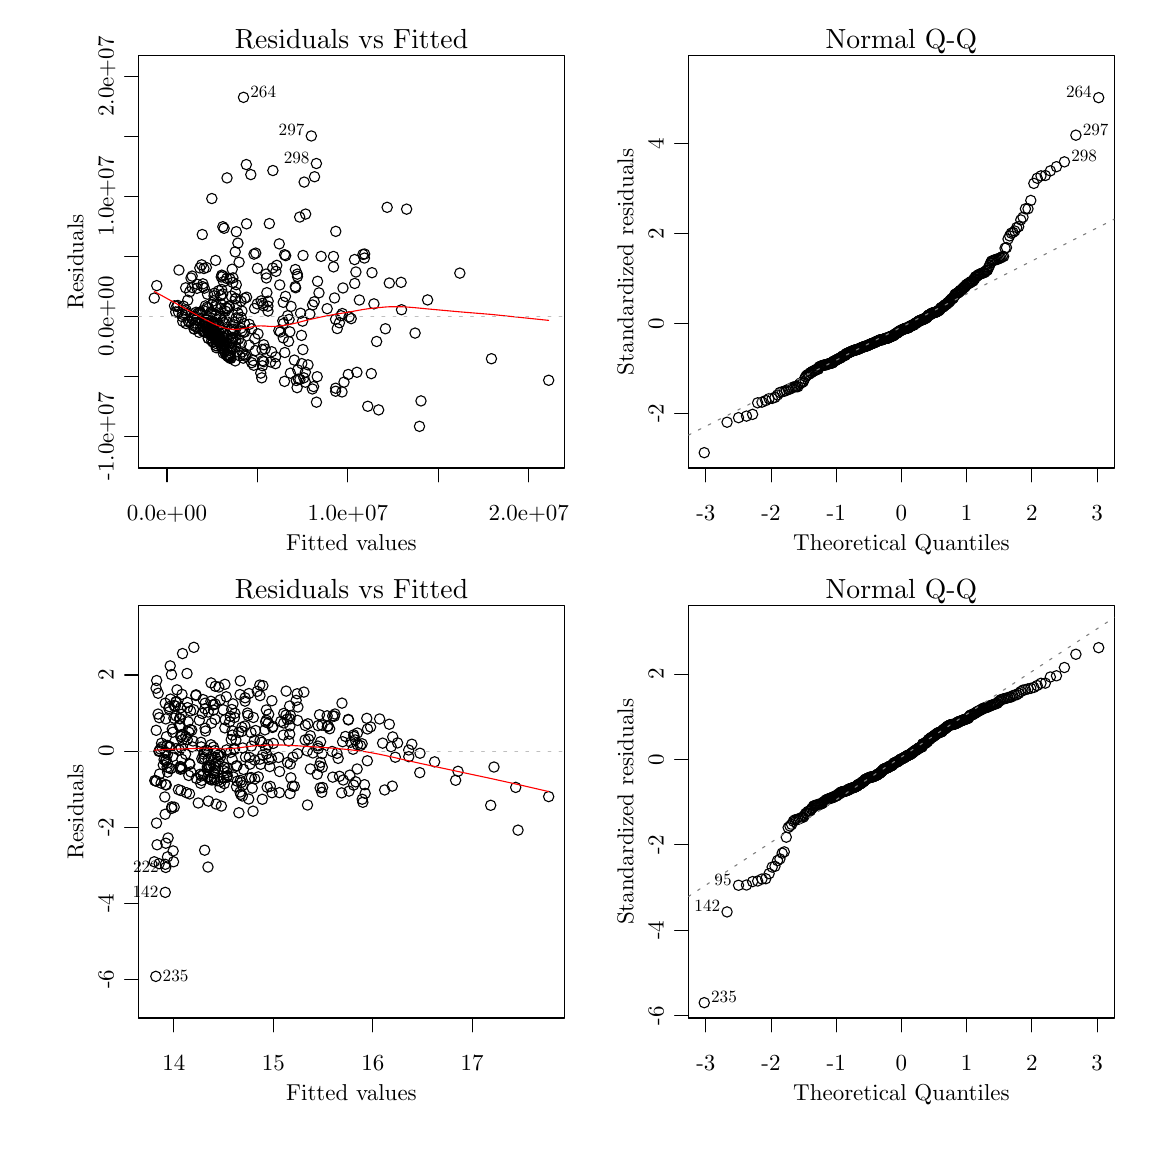
\begin{tikzpicture}[x=1pt,y=1pt]
\draw[color=white,opacity=0] (0,0) rectangle (397.48,397.48);
\begin{scope}
\path[clip] (  0.00,  0.00) rectangle (397.48,397.48);
\definecolor[named]{drawColor}{rgb}{0.75,0.90,0.18}
\definecolor[named]{drawColor}{rgb}{0.00,0.00,0.00}

\draw[color=drawColor,line cap=round,line join=round,fill opacity=0.00,] ( 50.14,238.58) -- (180.87,238.58);

\draw[color=drawColor,line cap=round,line join=round,fill opacity=0.00,] ( 50.14,238.58) -- ( 50.14,233.60);

\draw[color=drawColor,line cap=round,line join=round,fill opacity=0.00,] ( 82.82,238.58) -- ( 82.82,233.60);

\draw[color=drawColor,line cap=round,line join=round,fill opacity=0.00,] (115.50,238.58) -- (115.50,233.60);

\draw[color=drawColor,line cap=round,line join=round,fill opacity=0.00,] (148.19,238.58) -- (148.19,233.60);

\draw[color=drawColor,line cap=round,line join=round,fill opacity=0.00,] (180.87,238.58) -- (180.87,233.60);

\node[color=drawColor,anchor=base,inner sep=0pt, outer sep=0pt, scale=  0.83] at ( 50.14,219.66) {0.0e+00%
};

\node[color=drawColor,anchor=base,inner sep=0pt, outer sep=0pt, scale=  0.83] at (115.50,219.66) {1.0e+07%
};

\node[color=drawColor,anchor=base,inner sep=0pt, outer sep=0pt, scale=  0.83] at (180.87,219.66) {2.0e+07%
};

\draw[color=drawColor,line cap=round,line join=round,fill opacity=0.00,] ( 39.84,249.98) -- ( 39.84,380.07);

\draw[color=drawColor,line cap=round,line join=round,fill opacity=0.00,] ( 39.84,249.98) -- ( 34.86,249.98);

\draw[color=drawColor,line cap=round,line join=round,fill opacity=0.00,] ( 39.84,271.66) -- ( 34.86,271.66);

\draw[color=drawColor,line cap=round,line join=round,fill opacity=0.00,] ( 39.84,293.34) -- ( 34.86,293.34);

\draw[color=drawColor,line cap=round,line join=round,fill opacity=0.00,] ( 39.84,315.02) -- ( 34.86,315.02);

\draw[color=drawColor,line cap=round,line join=round,fill opacity=0.00,] ( 39.84,336.71) -- ( 34.86,336.71);

\draw[color=drawColor,line cap=round,line join=round,fill opacity=0.00,] ( 39.84,358.39) -- ( 34.86,358.39);

\draw[color=drawColor,line cap=round,line join=round,fill opacity=0.00,] ( 39.84,380.07) -- ( 34.86,380.07);

\node[rotate= 90.00,color=drawColor,anchor=base,inner sep=0pt, outer sep=0pt, scale=  0.83] at ( 30.88,249.98) {-1.0e+07%
};

\node[rotate= 90.00,color=drawColor,anchor=base,inner sep=0pt, outer sep=0pt, scale=  0.83] at ( 30.88,293.34) {0.0e+00%
};

\node[rotate= 90.00,color=drawColor,anchor=base,inner sep=0pt, outer sep=0pt, scale=  0.83] at ( 30.88,336.71) {1.0e+07%
};

\node[rotate= 90.00,color=drawColor,anchor=base,inner sep=0pt, outer sep=0pt, scale=  0.83] at ( 30.88,380.07) {2.0e+07%
};

\draw[color=drawColor,line cap=round,line join=round,fill opacity=0.00,] ( 39.84,238.58) --
	(193.76,238.58) --
	(193.76,387.53) --
	( 39.84,387.53) --
	( 39.84,238.58);
\end{scope}
\begin{scope}
\path[clip] (  0.00,198.74) rectangle (198.74,397.48);
\definecolor[named]{drawColor}{rgb}{0.75,0.90,0.18}
\definecolor[named]{drawColor}{rgb}{0.00,0.00,0.00}

\node[color=drawColor,anchor=base,inner sep=0pt, outer sep=0pt, scale=  0.83] at (116.80,208.70) {Fitted values%
};

\node[rotate= 90.00,color=drawColor,anchor=base,inner sep=0pt, outer sep=0pt, scale=  0.83] at ( 19.92,313.05) {Residuals%
};
\end{scope}
\begin{scope}
\path[clip] ( 39.84,238.58) rectangle (193.76,387.53);
\definecolor[named]{drawColor}{rgb}{0.75,0.90,0.18}
\definecolor[named]{drawColor}{rgb}{0.00,0.00,0.00}

\draw[color=drawColor,line cap=round,line join=round,fill opacity=0.00,] ( 81.23,277.42) circle (  1.87);

\draw[color=drawColor,line cap=round,line join=round,fill opacity=0.00,] ( 70.76,285.61) circle (  1.87);

\draw[color=drawColor,line cap=round,line join=round,fill opacity=0.00,] (118.77,273.15) circle (  1.87);

\draw[color=drawColor,line cap=round,line join=round,fill opacity=0.00,] ( 70.48,291.05) circle (  1.87);

\draw[color=drawColor,line cap=round,line join=round,fill opacity=0.00,] ( 52.85,297.18) circle (  1.87);

\draw[color=drawColor,line cap=round,line join=round,fill opacity=0.00,] ( 99.71,341.88) circle (  1.87);

\draw[color=drawColor,line cap=round,line join=round,fill opacity=0.00,] ( 57.64,299.21) circle (  1.87);

\draw[color=drawColor,line cap=round,line join=round,fill opacity=0.00,] ( 72.54,297.13) circle (  1.87);

\draw[color=drawColor,line cap=round,line join=round,fill opacity=0.00,] ( 65.98,286.54) circle (  1.87);

\draw[color=drawColor,line cap=round,line join=round,fill opacity=0.00,] ( 72.48,278.75) circle (  1.87);

\draw[color=drawColor,line cap=round,line join=round,fill opacity=0.00,] ( 80.72,288.88) circle (  1.87);

\draw[color=drawColor,line cap=round,line join=round,fill opacity=0.00,] ( 73.92,287.60) circle (  1.87);

\draw[color=drawColor,line cap=round,line join=round,fill opacity=0.00,] ( 64.65,289.43) circle (  1.87);

\draw[color=drawColor,line cap=round,line join=round,fill opacity=0.00,] (121.49,314.43) circle (  1.87);

\draw[color=drawColor,line cap=round,line join=round,fill opacity=0.00,] ( 45.54,299.97) circle (  1.87);

\draw[color=drawColor,line cap=round,line join=round,fill opacity=0.00,] (100.24,330.32) circle (  1.87);

\draw[color=drawColor,line cap=round,line join=round,fill opacity=0.00,] ( 98.74,286.48) circle (  1.87);

\draw[color=drawColor,line cap=round,line join=round,fill opacity=0.00,] ( 67.82,293.76) circle (  1.87);

\draw[color=drawColor,line cap=round,line join=round,fill opacity=0.00,] ( 72.51,283.31) circle (  1.87);

\draw[color=drawColor,line cap=round,line join=round,fill opacity=0.00,] ( 66.77,286.86) circle (  1.87);

\draw[color=drawColor,line cap=round,line join=round,fill opacity=0.00,] ( 68.09,291.73) circle (  1.87);

\draw[color=drawColor,line cap=round,line join=round,fill opacity=0.00,] ( 76.86,289.06) circle (  1.87);

\draw[color=drawColor,line cap=round,line join=round,fill opacity=0.00,] ( 68.93,290.04) circle (  1.87);

\draw[color=drawColor,line cap=round,line join=round,fill opacity=0.00,] ( 67.27,301.72) circle (  1.87);

\draw[color=drawColor,line cap=round,line join=round,fill opacity=0.00,] ( 72.89,306.87) circle (  1.87);

\draw[color=drawColor,line cap=round,line join=round,fill opacity=0.00,] (123.97,272.67) circle (  1.87);

\draw[color=drawColor,line cap=round,line join=round,fill opacity=0.00,] ( 84.72,277.33) circle (  1.87);

\draw[color=drawColor,line cap=round,line join=round,fill opacity=0.00,] ( 74.79,277.27) circle (  1.87);

\draw[color=drawColor,line cap=round,line join=round,fill opacity=0.00,] ( 60.98,303.49) circle (  1.87);

\draw[color=drawColor,line cap=round,line join=round,fill opacity=0.00,] ( 86.69,298.86) circle (  1.87);

\draw[color=drawColor,line cap=round,line join=round,fill opacity=0.00,] ( 69.75,307.62) circle (  1.87);

\draw[color=drawColor,line cap=round,line join=round,fill opacity=0.00,] ( 78.43,279.42) circle (  1.87);

\draw[color=drawColor,line cap=round,line join=round,fill opacity=0.00,] ( 79.79,282.96) circle (  1.87);

\draw[color=drawColor,line cap=round,line join=round,fill opacity=0.00,] ( 94.08,284.31) circle (  1.87);

\draw[color=drawColor,line cap=round,line join=round,fill opacity=0.00,] ( 62.80,291.65) circle (  1.87);

\draw[color=drawColor,line cap=round,line join=round,fill opacity=0.00,] ( 73.39,300.68) circle (  1.87);

\draw[color=drawColor,line cap=round,line join=round,fill opacity=0.00,] ( 66.37,286.15) circle (  1.87);

\draw[color=drawColor,line cap=round,line join=round,fill opacity=0.00,] ( 84.98,297.19) circle (  1.87);

\draw[color=drawColor,line cap=round,line join=round,fill opacity=0.00,] ( 82.82,310.69) circle (  1.87);

\draw[color=drawColor,line cap=round,line join=round,fill opacity=0.00,] (113.73,303.62) circle (  1.87);

\draw[color=drawColor,line cap=round,line join=round,fill opacity=0.00,] ( 69.03,284.50) circle (  1.87);

\draw[color=drawColor,line cap=round,line join=round,fill opacity=0.00,] ( 77.22,295.28) circle (  1.87);

\draw[color=drawColor,line cap=round,line join=round,fill opacity=0.00,] ( 78.24,287.71) circle (  1.87);

\draw[color=drawColor,line cap=round,line join=round,fill opacity=0.00,] ( 64.76,288.12) circle (  1.87);

\draw[color=drawColor,line cap=round,line join=round,fill opacity=0.00,] (116.71,292.54) circle (  1.87);

\draw[color=drawColor,line cap=round,line join=round,fill opacity=0.00,] ( 74.60,291.28) circle (  1.87);

\draw[color=drawColor,line cap=round,line join=round,fill opacity=0.00,] ( 61.78,294.54) circle (  1.87);

\draw[color=drawColor,line cap=round,line join=round,fill opacity=0.00,] (139.79,287.31) circle (  1.87);

\draw[color=drawColor,line cap=round,line join=round,fill opacity=0.00,] (144.31,299.30) circle (  1.87);

\draw[color=drawColor,line cap=round,line join=round,fill opacity=0.00,] ( 72.71,279.28) circle (  1.87);

\draw[color=drawColor,line cap=round,line join=round,fill opacity=0.00,] ( 63.01,289.97) circle (  1.87);

\draw[color=drawColor,line cap=round,line join=round,fill opacity=0.00,] ( 71.83,343.39) circle (  1.87);

\draw[color=drawColor,line cap=round,line join=round,fill opacity=0.00,] ( 77.19,288.04) circle (  1.87);

\draw[color=drawColor,line cap=round,line join=round,fill opacity=0.00,] ( 70.22,291.80) circle (  1.87);

\draw[color=drawColor,line cap=round,line join=round,fill opacity=0.00,] ( 68.34,286.07) circle (  1.87);

\draw[color=drawColor,line cap=round,line join=round,fill opacity=0.00,] ( 59.92,288.83) circle (  1.87);

\draw[color=drawColor,line cap=round,line join=round,fill opacity=0.00,] (104.16,262.35) circle (  1.87);

\draw[color=drawColor,line cap=round,line join=round,fill opacity=0.00,] ( 70.11,284.90) circle (  1.87);

\draw[color=drawColor,line cap=round,line join=round,fill opacity=0.00,] ( 55.82,291.56) circle (  1.87);

\draw[color=drawColor,line cap=round,line join=round,fill opacity=0.00,] ( 72.00,296.18) circle (  1.87);

\draw[color=drawColor,line cap=round,line join=round,fill opacity=0.00,] ( 70.83,283.07) circle (  1.87);

\draw[color=drawColor,line cap=round,line join=round,fill opacity=0.00,] (129.70,332.76) circle (  1.87);

\draw[color=drawColor,line cap=round,line join=round,fill opacity=0.00,] ( 81.49,275.69) circle (  1.87);

\draw[color=drawColor,line cap=round,line join=round,fill opacity=0.00,] ( 75.77,319.83) circle (  1.87);

\draw[color=drawColor,line cap=round,line join=round,fill opacity=0.00,] ( 97.38,274.01) circle (  1.87);

\draw[color=drawColor,line cap=round,line join=round,fill opacity=0.00,] ( 80.75,276.61) circle (  1.87);

\draw[color=drawColor,line cap=round,line join=round,fill opacity=0.00,] ( 92.96,300.57) circle (  1.87);

\draw[color=drawColor,line cap=round,line join=round,fill opacity=0.00,] ( 74.80,316.66) circle (  1.87);

\draw[color=drawColor,line cap=round,line join=round,fill opacity=0.00,] ( 66.64,286.10) circle (  1.87);

\draw[color=drawColor,line cap=round,line join=round,fill opacity=0.00,] ( 54.30,294.96) circle (  1.87);

\draw[color=drawColor,line cap=round,line join=round,fill opacity=0.00,] ( 63.12,305.11) circle (  1.87);

\draw[color=drawColor,line cap=round,line join=round,fill opacity=0.00,] ( 58.51,293.45) circle (  1.87);

\draw[color=drawColor,line cap=round,line join=round,fill opacity=0.00,] (121.56,315.88) circle (  1.87);

\draw[color=drawColor,line cap=round,line join=round,fill opacity=0.00,] ( 84.65,275.51) circle (  1.87);

\draw[color=drawColor,line cap=round,line join=round,fill opacity=0.00,] ( 61.27,289.23) circle (  1.87);

\draw[color=drawColor,line cap=round,line join=round,fill opacity=0.00,] ( 66.34,335.93) circle (  1.87);

\draw[color=drawColor,line cap=round,line join=round,fill opacity=0.00,] ( 97.15,267.60) circle (  1.87);

\draw[color=drawColor,line cap=round,line join=round,fill opacity=0.00,] ( 56.10,297.04) circle (  1.87);

\draw[color=drawColor,line cap=round,line join=round,fill opacity=0.00,] ( 68.70,286.52) circle (  1.87);

\draw[color=drawColor,line cap=round,line join=round,fill opacity=0.00,] ( 63.29,289.74) circle (  1.87);

\draw[color=drawColor,line cap=round,line join=round,fill opacity=0.00,] ( 64.10,289.21) circle (  1.87);

\draw[color=drawColor,line cap=round,line join=round,fill opacity=0.00,] ( 55.71,294.13) circle (  1.87);

\draw[color=drawColor,line cap=round,line join=round,fill opacity=0.00,] ( 64.36,311.01) circle (  1.87);

\draw[color=drawColor,line cap=round,line join=round,fill opacity=0.00,] ( 79.86,290.46) circle (  1.87);

\draw[color=drawColor,line cap=round,line join=round,fill opacity=0.00,] ( 72.06,279.17) circle (  1.87);

\draw[color=drawColor,line cap=round,line join=round,fill opacity=0.00,] ( 67.67,296.89) circle (  1.87);

\draw[color=drawColor,line cap=round,line join=round,fill opacity=0.00,] (103.35,298.63) circle (  1.87);

\draw[color=drawColor,line cap=round,line join=round,fill opacity=0.00,] ( 60.01,288.78) circle (  1.87);

\draw[color=drawColor,line cap=round,line join=round,fill opacity=0.00,] ( 70.78,325.18) circle (  1.87);

\draw[color=drawColor,line cap=round,line join=round,fill opacity=0.00,] ( 85.59,281.57) circle (  1.87);

\draw[color=drawColor,line cap=round,line join=round,fill opacity=0.00,] ( 78.90,326.80) circle (  1.87);

\draw[color=drawColor,line cap=round,line join=round,fill opacity=0.00,] ( 65.31,291.90) circle (  1.87);

\draw[color=drawColor,line cap=round,line join=round,fill opacity=0.00,] (104.55,306.03) circle (  1.87);

\draw[color=drawColor,line cap=round,line join=round,fill opacity=0.00,] ( 64.02,297.14) circle (  1.87);

\draw[color=drawColor,line cap=round,line join=round,fill opacity=0.00,] ( 72.86,278.61) circle (  1.87);

\draw[color=drawColor,line cap=round,line join=round,fill opacity=0.00,] ( 66.17,292.68) circle (  1.87);

\draw[color=drawColor,line cap=round,line join=round,fill opacity=0.00,] ( 63.90,291.49) circle (  1.87);

\draw[color=drawColor,line cap=round,line join=round,fill opacity=0.00,] ( 92.71,280.28) circle (  1.87);

\draw[color=drawColor,line cap=round,line join=round,fill opacity=0.00,] (105.06,301.86) circle (  1.87);

\draw[color=drawColor,line cap=round,line join=round,fill opacity=0.00,] ( 72.96,288.19) circle (  1.87);

\draw[color=drawColor,line cap=round,line join=round,fill opacity=0.00,] ( 70.95,283.38) circle (  1.87);

\draw[color=drawColor,line cap=round,line join=round,fill opacity=0.00,] ( 85.92,308.63) circle (  1.87);

\draw[color=drawColor,line cap=round,line join=round,fill opacity=0.00,] ( 71.91,286.45) circle (  1.87);

\draw[color=drawColor,line cap=round,line join=round,fill opacity=0.00,] ( 63.48,310.65) circle (  1.87);

\draw[color=drawColor,line cap=round,line join=round,fill opacity=0.00,] ( 66.51,297.66) circle (  1.87);

\draw[color=drawColor,line cap=round,line join=round,fill opacity=0.00,] ( 66.98,286.49) circle (  1.87);

\draw[color=drawColor,line cap=round,line join=round,fill opacity=0.00,] ( 69.58,288.40) circle (  1.87);

\draw[color=drawColor,line cap=round,line join=round,fill opacity=0.00,] ( 60.71,292.00) circle (  1.87);

\draw[color=drawColor,line cap=round,line join=round,fill opacity=0.00,] ( 82.75,297.87) circle (  1.87);

\draw[color=drawColor,line cap=round,line join=round,fill opacity=0.00,] (136.73,332.10) circle (  1.87);

\draw[color=drawColor,line cap=round,line join=round,fill opacity=0.00,] ( 89.52,309.63) circle (  1.87);

\draw[color=drawColor,line cap=round,line join=round,fill opacity=0.00,] (141.38,253.61) circle (  1.87);

\draw[color=drawColor,line cap=round,line join=round,fill opacity=0.00,] ( 60.32,290.94) circle (  1.87);

\draw[color=drawColor,line cap=round,line join=round,fill opacity=0.00,] ( 96.52,310.28) circle (  1.87);

\draw[color=drawColor,line cap=round,line join=round,fill opacity=0.00,] ( 73.24,285.39) circle (  1.87);

\draw[color=drawColor,line cap=round,line join=round,fill opacity=0.00,] ( 63.25,295.48) circle (  1.87);

\draw[color=drawColor,line cap=round,line join=round,fill opacity=0.00,] ( 70.31,301.47) circle (  1.87);

\draw[color=drawColor,line cap=round,line join=round,fill opacity=0.00,] (122.69,260.87) circle (  1.87);

\draw[color=drawColor,line cap=round,line join=round,fill opacity=0.00,] ( 66.26,287.33) circle (  1.87);

\draw[color=drawColor,line cap=round,line join=round,fill opacity=0.00,] ( 81.78,296.20) circle (  1.87);

\draw[color=drawColor,line cap=round,line join=round,fill opacity=0.00,] ( 65.68,288.08) circle (  1.87);

\draw[color=drawColor,line cap=round,line join=round,fill opacity=0.00,] ( 63.81,288.04) circle (  1.87);

\draw[color=drawColor,line cap=round,line join=round,fill opacity=0.00,] ( 67.84,292.44) circle (  1.87);

\draw[color=drawColor,line cap=round,line join=round,fill opacity=0.00,] ( 69.56,300.84) circle (  1.87);

\draw[color=drawColor,line cap=round,line join=round,fill opacity=0.00,] ( 69.44,293.41) circle (  1.87);

\draw[color=drawColor,line cap=round,line join=round,fill opacity=0.00,] ( 76.19,312.92) circle (  1.87);

\draw[color=drawColor,line cap=round,line join=round,fill opacity=0.00,] ( 70.55,305.85) circle (  1.87);

\draw[color=drawColor,line cap=round,line join=round,fill opacity=0.00,] ( 83.04,287.02) circle (  1.87);

\draw[color=drawColor,line cap=round,line join=round,fill opacity=0.00,] (102.67,267.12) circle (  1.87);

\draw[color=drawColor,line cap=round,line join=round,fill opacity=0.00,] ( 67.92,282.72) circle (  1.87);

\draw[color=drawColor,line cap=round,line join=round,fill opacity=0.00,] (111.08,266.31) circle (  1.87);

\draw[color=drawColor,line cap=round,line join=round,fill opacity=0.00,] ( 74.83,302.11) circle (  1.87);

\draw[color=drawColor,line cap=round,line join=round,fill opacity=0.00,] (111.13,324.07) circle (  1.87);

\draw[color=drawColor,line cap=round,line join=round,fill opacity=0.00,] (111.08,267.40) circle (  1.87);

\draw[color=drawColor,line cap=round,line join=round,fill opacity=0.00,] (117.92,313.88) circle (  1.87);

\draw[color=drawColor,line cap=round,line join=round,fill opacity=0.00,] (104.42,271.56) circle (  1.87);

\draw[color=drawColor,line cap=round,line join=round,fill opacity=0.00,] ( 70.45,280.10) circle (  1.87);

\draw[color=drawColor,line cap=round,line join=round,fill opacity=0.00,] ( 66.89,289.90) circle (  1.87);

\draw[color=drawColor,line cap=round,line join=round,fill opacity=0.00,] ( 64.77,301.36) circle (  1.87);

\draw[color=drawColor,line cap=round,line join=round,fill opacity=0.00,] ( 77.71,279.56) circle (  1.87);

\draw[color=drawColor,line cap=round,line join=round,fill opacity=0.00,] ( 70.27,284.45) circle (  1.87);

\draw[color=drawColor,line cap=round,line join=round,fill opacity=0.00,] ( 72.15,278.86) circle (  1.87);

\draw[color=drawColor,line cap=round,line join=round,fill opacity=0.00,] ( 97.24,308.61) circle (  1.87);

\draw[color=drawColor,line cap=round,line join=round,fill opacity=0.00,] ( 81.58,315.85) circle (  1.87);

\draw[color=drawColor,line cap=round,line join=round,fill opacity=0.00,] ( 89.37,278.69) circle (  1.87);

\draw[color=drawColor,line cap=round,line join=round,fill opacity=0.00,] ( 62.00,310.86) circle (  1.87);

\draw[color=drawColor,line cap=round,line join=round,fill opacity=0.00,] ( 62.14,288.96) circle (  1.87);

\draw[color=drawColor,line cap=round,line join=round,fill opacity=0.00,] (113.49,294.38) circle (  1.87);

\draw[color=drawColor,line cap=round,line join=round,fill opacity=0.00,] ( 65.26,287.65) circle (  1.87);

\draw[color=drawColor,line cap=round,line join=round,fill opacity=0.00,] ( 65.01,285.46) circle (  1.87);

\draw[color=drawColor,line cap=round,line join=round,fill opacity=0.00,] ( 73.63,281.97) circle (  1.87);

\draw[color=drawColor,line cap=round,line join=round,fill opacity=0.00,] ( 98.85,276.28) circle (  1.87);

\draw[color=drawColor,line cap=round,line join=round,fill opacity=0.00,] ( 78.13,290.74) circle (  1.87);

\draw[color=drawColor,line cap=round,line join=round,fill opacity=0.00,] ( 70.74,281.66) circle (  1.87);

\draw[color=drawColor,line cap=round,line join=round,fill opacity=0.00,] ( 62.35,292.61) circle (  1.87);

\draw[color=drawColor,line cap=round,line join=round,fill opacity=0.00,] ( 60.53,289.64) circle (  1.87);

\draw[color=drawColor,line cap=round,line join=round,fill opacity=0.00,] ( 69.78,284.02) circle (  1.87);

\draw[color=drawColor,line cap=round,line join=round,fill opacity=0.00,] ( 93.03,315.30) circle (  1.87);

\draw[color=drawColor,line cap=round,line join=round,fill opacity=0.00,] ( 75.01,284.90) circle (  1.87);

\draw[color=drawColor,line cap=round,line join=round,fill opacity=0.00,] ( 76.92,292.94) circle (  1.87);

\draw[color=drawColor,line cap=round,line join=round,fill opacity=0.00,] (115.94,293.17) circle (  1.87);

\draw[color=drawColor,line cap=round,line join=round,fill opacity=0.00,] (111.66,288.95) circle (  1.87);

\draw[color=drawColor,line cap=round,line join=round,fill opacity=0.00,] ( 99.13,291.63) circle (  1.87);

\draw[color=drawColor,line cap=round,line join=round,fill opacity=0.00,] ( 61.09,304.94) circle (  1.87);

\draw[color=drawColor,line cap=round,line join=round,fill opacity=0.00,] ( 62.42,294.38) circle (  1.87);

\draw[color=drawColor,line cap=round,line join=round,fill opacity=0.00,] ( 76.02,285.12) circle (  1.87);

\draw[color=drawColor,line cap=round,line join=round,fill opacity=0.00,] ( 78.90,300.28) circle (  1.87);

\draw[color=drawColor,line cap=round,line join=round,fill opacity=0.00,] ( 69.32,284.45) circle (  1.87);

\draw[color=drawColor,line cap=round,line join=round,fill opacity=0.00,] ( 60.67,294.84) circle (  1.87);

\draw[color=drawColor,line cap=round,line join=round,fill opacity=0.00,] ( 85.10,276.98) circle (  1.87);

\draw[color=drawColor,line cap=round,line join=round,fill opacity=0.00,] ( 73.68,283.92) circle (  1.87);

\draw[color=drawColor,line cap=round,line join=round,fill opacity=0.00,] (113.01,293.61) circle (  1.87);

\draw[color=drawColor,line cap=round,line join=round,fill opacity=0.00,] ( 92.61,269.86) circle (  1.87);

\draw[color=drawColor,line cap=round,line join=round,fill opacity=0.00,] (100.15,273.17) circle (  1.87);

\draw[color=drawColor,line cap=round,line join=round,fill opacity=0.00,] ( 73.62,288.53) circle (  1.87);

\draw[color=drawColor,line cap=round,line join=round,fill opacity=0.00,] ( 96.62,303.70) circle (  1.87);

\draw[color=drawColor,line cap=round,line join=round,fill opacity=0.00,] ( 54.07,297.30) circle (  1.87);

\draw[color=drawColor,line cap=round,line join=round,fill opacity=0.00,] ( 62.13,294.85) circle (  1.87);

\draw[color=drawColor,line cap=round,line join=round,fill opacity=0.00,] (114.10,269.59) circle (  1.87);

\draw[color=drawColor,line cap=round,line join=round,fill opacity=0.00,] ( 71.54,291.55) circle (  1.87);

\draw[color=drawColor,line cap=round,line join=round,fill opacity=0.00,] (167.38,278.05) circle (  1.87);

\draw[color=drawColor,line cap=round,line join=round,fill opacity=0.00,] ( 75.19,323.95) circle (  1.87);

\draw[color=drawColor,line cap=round,line join=round,fill opacity=0.00,] ( 65.89,288.56) circle (  1.87);

\draw[color=drawColor,line cap=round,line join=round,fill opacity=0.00,] ( 71.01,280.63) circle (  1.87);

\draw[color=drawColor,line cap=round,line join=round,fill opacity=0.00,] ( 77.75,287.60) circle (  1.87);

\draw[color=drawColor,line cap=round,line join=round,fill opacity=0.00,] ( 66.71,284.05) circle (  1.87);

\draw[color=drawColor,line cap=round,line join=round,fill opacity=0.00,] ( 70.31,285.62) circle (  1.87);

\draw[color=drawColor,line cap=round,line join=round,fill opacity=0.00,] ( 70.16,281.48) circle (  1.87);

\draw[color=drawColor,line cap=round,line join=round,fill opacity=0.00,] ( 67.89,297.59) circle (  1.87);

\draw[color=drawColor,line cap=round,line join=round,fill opacity=0.00,] ( 68.01,286.18) circle (  1.87);

\draw[color=drawColor,line cap=round,line join=round,fill opacity=0.00,] (124.92,297.88) circle (  1.87);

\draw[color=drawColor,line cap=round,line join=round,fill opacity=0.00,] ( 77.27,280.50) circle (  1.87);

\draw[color=drawColor,line cap=round,line join=round,fill opacity=0.00,] ( 98.18,270.58) circle (  1.87);

\draw[color=drawColor,line cap=round,line join=round,fill opacity=0.00,] ( 78.58,278.94) circle (  1.87);

\draw[color=drawColor,line cap=round,line join=round,fill opacity=0.00,] ( 65.37,287.79) circle (  1.87);

\draw[color=drawColor,line cap=round,line join=round,fill opacity=0.00,] ( 90.55,288.21) circle (  1.87);

\draw[color=drawColor,line cap=round,line join=round,fill opacity=0.00,] ( 60.44,289.70) circle (  1.87);

\draw[color=drawColor,line cap=round,line join=round,fill opacity=0.00,] ( 98.41,294.49) circle (  1.87);

\draw[color=drawColor,line cap=round,line join=round,fill opacity=0.00,] (188.06,270.27) circle (  1.87);

\draw[color=drawColor,line cap=round,line join=round,fill opacity=0.00,] ( 71.75,307.05) circle (  1.87);

\draw[color=drawColor,line cap=round,line join=round,fill opacity=0.00,] ( 92.63,315.64) circle (  1.87);

\draw[color=drawColor,line cap=round,line join=round,fill opacity=0.00,] ( 59.87,290.08) circle (  1.87);

\draw[color=drawColor,line cap=round,line join=round,fill opacity=0.00,] (119.66,299.26) circle (  1.87);

\draw[color=drawColor,line cap=round,line join=round,fill opacity=0.00,] ( 67.95,282.03) circle (  1.87);

\draw[color=drawColor,line cap=round,line join=round,fill opacity=0.00,] (110.30,315.01) circle (  1.87);

\draw[color=drawColor,line cap=round,line join=round,fill opacity=0.00,] ( 70.34,307.98) circle (  1.87);

\draw[color=drawColor,line cap=round,line join=round,fill opacity=0.00,] (100.15,269.57) circle (  1.87);

\draw[color=drawColor,line cap=round,line join=round,fill opacity=0.00,] ( 67.87,283.56) circle (  1.87);

\draw[color=drawColor,line cap=round,line join=round,fill opacity=0.00,] ( 85.09,283.10) circle (  1.87);

\draw[color=drawColor,line cap=round,line join=round,fill opacity=0.00,] ( 69.63,296.31) circle (  1.87);

\draw[color=drawColor,line cap=round,line join=round,fill opacity=0.00,] ( 67.09,290.34) circle (  1.87);

\draw[color=drawColor,line cap=round,line join=round,fill opacity=0.00,] ( 57.06,295.66) circle (  1.87);

\draw[color=drawColor,line cap=round,line join=round,fill opacity=0.00,] (124.22,309.14) circle (  1.87);

\draw[color=drawColor,line cap=round,line join=round,fill opacity=0.00,] ( 84.46,281.41) circle (  1.87);

\draw[color=drawColor,line cap=round,line join=round,fill opacity=0.00,] ( 72.51,278.72) circle (  1.87);

\draw[color=drawColor,line cap=round,line join=round,fill opacity=0.00,] ( 67.14,300.80) circle (  1.87);

\draw[color=drawColor,line cap=round,line join=round,fill opacity=0.00,] ( 63.81,291.30) circle (  1.87);

\draw[color=drawColor,line cap=round,line join=round,fill opacity=0.00,] ( 71.79,281.36) circle (  1.87);

\draw[color=drawColor,line cap=round,line join=round,fill opacity=0.00,] (108.02,296.14) circle (  1.87);

\draw[color=drawColor,line cap=round,line join=round,fill opacity=0.00,] ( 62.65,311.98) circle (  1.87);

\draw[color=drawColor,line cap=round,line join=round,fill opacity=0.00,] (101.77,294.21) circle (  1.87);

\draw[color=drawColor,line cap=round,line join=round,fill opacity=0.00,] ( 80.43,344.59) circle (  1.87);

\draw[color=drawColor,line cap=round,line join=round,fill opacity=0.00,] ( 69.89,303.07) circle (  1.87);

\draw[color=drawColor,line cap=round,line join=round,fill opacity=0.00,] ( 59.35,292.49) circle (  1.87);

\draw[color=drawColor,line cap=round,line join=round,fill opacity=0.00,] ( 74.84,299.75) circle (  1.87);

\draw[color=drawColor,line cap=round,line join=round,fill opacity=0.00,] ( 73.10,278.12) circle (  1.87);

\draw[color=drawColor,line cap=round,line join=round,fill opacity=0.00,] ( 81.90,285.28) circle (  1.87);

\draw[color=drawColor,line cap=round,line join=round,fill opacity=0.00,] ( 72.87,280.25) circle (  1.87);

\draw[color=drawColor,line cap=round,line join=round,fill opacity=0.00,] ( 67.40,288.13) circle (  1.87);

\draw[color=drawColor,line cap=round,line join=round,fill opacity=0.00,] ( 74.96,282.35) circle (  1.87);

\draw[color=drawColor,line cap=round,line join=round,fill opacity=0.00,] (141.92,262.81) circle (  1.87);

\draw[color=drawColor,line cap=round,line join=round,fill opacity=0.00,] ( 88.41,346.05) circle (  1.87);

\draw[color=drawColor,line cap=round,line join=round,fill opacity=0.00,] (103.11,267.98) circle (  1.87);

\draw[color=drawColor,line cap=round,line join=round,fill opacity=0.00,] ( 73.70,285.28) circle (  1.87);

\draw[color=drawColor,line cap=round,line join=round,fill opacity=0.00,] ( 96.16,277.56) circle (  1.87);

\draw[color=drawColor,line cap=round,line join=round,fill opacity=0.00,] ( 82.09,280.97) circle (  1.87);

\draw[color=drawColor,line cap=round,line join=round,fill opacity=0.00,] ( 69.01,285.97) circle (  1.87);

\draw[color=drawColor,line cap=round,line join=round,fill opacity=0.00,] ( 69.15,285.02) circle (  1.87);

\draw[color=drawColor,line cap=round,line join=round,fill opacity=0.00,] ( 75.19,304.80) circle (  1.87);

\draw[color=drawColor,line cap=round,line join=round,fill opacity=0.00,] ( 67.85,286.74) circle (  1.87);

\draw[color=drawColor,line cap=round,line join=round,fill opacity=0.00,] ( 73.26,278.38) circle (  1.87);

\draw[color=drawColor,line cap=round,line join=round,fill opacity=0.00,] ( 98.09,329.24) circle (  1.87);

\draw[color=drawColor,line cap=round,line join=round,fill opacity=0.00,] ( 82.21,316.21) circle (  1.87);

\draw[color=drawColor,line cap=round,line join=round,fill opacity=0.00,] ( 71.41,279.53) circle (  1.87);

\draw[color=drawColor,line cap=round,line join=round,fill opacity=0.00,] ( 75.89,292.65) circle (  1.87);

\draw[color=drawColor,line cap=round,line join=round,fill opacity=0.00,] ( 66.30,284.60) circle (  1.87);

\draw[color=drawColor,line cap=round,line join=round,fill opacity=0.00,] ( 68.83,302.62) circle (  1.87);

\draw[color=drawColor,line cap=round,line join=round,fill opacity=0.00,] ( 68.85,286.65) circle (  1.87);

\draw[color=drawColor,line cap=round,line join=round,fill opacity=0.00,] ( 92.14,285.59) circle (  1.87);

\draw[color=drawColor,line cap=round,line join=round,fill opacity=0.00,] ( 63.45,288.09) circle (  1.87);

\draw[color=drawColor,line cap=round,line join=round,fill opacity=0.00,] ( 58.02,291.31) circle (  1.87);

\draw[color=drawColor,line cap=round,line join=round,fill opacity=0.00,] ( 69.06,287.28) circle (  1.87);

\draw[color=drawColor,line cap=round,line join=round,fill opacity=0.00,] ( 77.79,372.50) circle (  1.87);

\draw[color=drawColor,line cap=round,line join=round,fill opacity=0.00,] ( 68.48,284.75) circle (  1.87);

\draw[color=drawColor,line cap=round,line join=round,fill opacity=0.00,] ( 69.57,284.03) circle (  1.87);

\draw[color=drawColor,line cap=round,line join=round,fill opacity=0.00,] ( 72.75,281.16) circle (  1.87);

\draw[color=drawColor,line cap=round,line join=round,fill opacity=0.00,] ( 75.12,292.81) circle (  1.87);

\draw[color=drawColor,line cap=round,line join=round,fill opacity=0.00,] ( 73.71,310.40) circle (  1.87);

\draw[color=drawColor,line cap=round,line join=round,fill opacity=0.00,] ( 93.75,293.60) circle (  1.87);

\draw[color=drawColor,line cap=round,line join=round,fill opacity=0.00,] ( 90.70,319.55) circle (  1.87);

\draw[color=drawColor,line cap=round,line join=round,fill opacity=0.00,] ( 88.36,310.83) circle (  1.87);

\draw[color=drawColor,line cap=round,line join=round,fill opacity=0.00,] ( 94.97,296.96) circle (  1.87);

\draw[color=drawColor,line cap=round,line join=round,fill opacity=0.00,] ( 69.96,282.18) circle (  1.87);

\draw[color=drawColor,line cap=round,line join=round,fill opacity=0.00,] ( 73.91,305.61) circle (  1.87);

\draw[color=drawColor,line cap=round,line join=round,fill opacity=0.00,] ( 70.75,292.68) circle (  1.87);

\draw[color=drawColor,line cap=round,line join=round,fill opacity=0.00,] ( 70.16,285.73) circle (  1.87);

\draw[color=drawColor,line cap=round,line join=round,fill opacity=0.00,] ( 65.06,287.15) circle (  1.87);

\draw[color=drawColor,line cap=round,line join=round,fill opacity=0.00,] ( 76.43,279.10) circle (  1.87);

\draw[color=drawColor,line cap=round,line join=round,fill opacity=0.00,] ( 67.56,286.64) circle (  1.87);

\draw[color=drawColor,line cap=round,line join=round,fill opacity=0.00,] (129.07,288.88) circle (  1.87);

\draw[color=drawColor,line cap=round,line join=round,fill opacity=0.00,] ( 65.20,296.36) circle (  1.87);

\draw[color=drawColor,line cap=round,line join=round,fill opacity=0.00,] (117.98,305.25) circle (  1.87);

\draw[color=drawColor,line cap=round,line join=round,fill opacity=0.00,] ( 92.15,298.43) circle (  1.87);

\draw[color=drawColor,line cap=round,line join=round,fill opacity=0.00,] ( 61.31,294.56) circle (  1.87);

\draw[color=drawColor,line cap=round,line join=round,fill opacity=0.00,] ( 99.59,271.14) circle (  1.87);

\draw[color=drawColor,line cap=round,line join=round,fill opacity=0.00,] ( 57.97,291.61) circle (  1.87);

\draw[color=drawColor,line cap=round,line join=round,fill opacity=0.00,] (155.96,308.98) circle (  1.87);

\draw[color=drawColor,line cap=round,line join=round,fill opacity=0.00,] ( 69.43,284.25) circle (  1.87);

\draw[color=drawColor,line cap=round,line join=round,fill opacity=0.00,] ( 76.86,298.86) circle (  1.87);

\draw[color=drawColor,line cap=round,line join=round,fill opacity=0.00,] (118.41,309.40) circle (  1.87);

\draw[color=drawColor,line cap=round,line join=round,fill opacity=0.00,] ( 97.29,307.76) circle (  1.87);

\draw[color=drawColor,line cap=round,line join=round,fill opacity=0.00,] (102.74,297.47) circle (  1.87);

\draw[color=drawColor,line cap=round,line join=round,fill opacity=0.00,] ( 64.44,289.52) circle (  1.87);

\draw[color=drawColor,line cap=round,line join=round,fill opacity=0.00,] (102.30,358.55) circle (  1.87);

\draw[color=drawColor,line cap=round,line join=round,fill opacity=0.00,] (104.13,348.59) circle (  1.87);

\draw[color=drawColor,line cap=round,line join=round,fill opacity=0.00,] ( 71.59,296.45) circle (  1.87);

\draw[color=drawColor,line cap=round,line join=round,fill opacity=0.00,] ( 59.23,307.91) circle (  1.87);

\draw[color=drawColor,line cap=round,line join=round,fill opacity=0.00,] ( 62.28,293.91) circle (  1.87);

\draw[color=drawColor,line cap=round,line join=round,fill opacity=0.00,] ( 74.37,288.73) circle (  1.87);

\draw[color=drawColor,line cap=round,line join=round,fill opacity=0.00,] ( 99.30,315.36) circle (  1.87);

\draw[color=drawColor,line cap=round,line join=round,fill opacity=0.00,] (105.83,315.03) circle (  1.87);

\draw[color=drawColor,line cap=round,line join=round,fill opacity=0.00,] ( 59.78,293.45) circle (  1.87);

\draw[color=drawColor,line cap=round,line join=round,fill opacity=0.00,] ( 64.37,290.61) circle (  1.87);

\draw[color=drawColor,line cap=round,line join=round,fill opacity=0.00,] ( 65.13,285.38) circle (  1.87);

\draw[color=drawColor,line cap=round,line join=round,fill opacity=0.00,] ( 99.25,281.36) circle (  1.87);

\draw[color=drawColor,line cap=round,line join=round,fill opacity=0.00,] ( 78.22,299.87) circle (  1.87);

\draw[color=drawColor,line cap=round,line join=round,fill opacity=0.00,] ( 68.23,285.18) circle (  1.87);

\draw[color=drawColor,line cap=round,line join=round,fill opacity=0.00,] (103.46,343.81) circle (  1.87);

\draw[color=drawColor,line cap=round,line join=round,fill opacity=0.00,] ( 74.98,299.81) circle (  1.87);

\draw[color=drawColor,line cap=round,line join=round,fill opacity=0.00,] ( 91.98,291.74) circle (  1.87);

\draw[color=drawColor,line cap=round,line join=round,fill opacity=0.00,] ( 73.04,281.86) circle (  1.87);

\draw[color=drawColor,line cap=round,line join=round,fill opacity=0.00,] ( 53.29,294.96) circle (  1.87);

\draw[color=drawColor,line cap=round,line join=round,fill opacity=0.00,] ( 66.87,284.22) circle (  1.87);

\draw[color=drawColor,line cap=round,line join=round,fill opacity=0.00,] ( 56.88,294.29) circle (  1.87);

\draw[color=drawColor,line cap=round,line join=round,fill opacity=0.00,] ( 89.82,311.79) circle (  1.87);

\draw[color=drawColor,line cap=round,line join=round,fill opacity=0.00,] ( 73.96,307.27) circle (  1.87);

\draw[color=drawColor,line cap=round,line join=round,fill opacity=0.00,] ( 64.99,288.15) circle (  1.87);

\draw[color=drawColor,line cap=round,line join=round,fill opacity=0.00,] ( 69.93,308.25) circle (  1.87);

\draw[color=drawColor,line cap=round,line join=round,fill opacity=0.00,] ( 76.99,283.50) circle (  1.87);

\draw[color=drawColor,line cap=round,line join=round,fill opacity=0.00,] ( 71.89,279.34) circle (  1.87);

\draw[color=drawColor,line cap=round,line join=round,fill opacity=0.00,] (120.94,315.75) circle (  1.87);

\draw[color=drawColor,line cap=round,line join=round,fill opacity=0.00,] ( 68.06,287.12) circle (  1.87);

\draw[color=drawColor,line cap=round,line join=round,fill opacity=0.00,] ( 78.81,348.21) circle (  1.87);

\draw[color=drawColor,line cap=round,line join=round,fill opacity=0.00,] ( 87.96,280.57) circle (  1.87);

\draw[color=drawColor,line cap=round,line join=round,fill opacity=0.00,] ( 67.86,282.79) circle (  1.87);

\draw[color=drawColor,line cap=round,line join=round,fill opacity=0.00,] (110.32,311.24) circle (  1.87);

\draw[color=drawColor,line cap=round,line join=round,fill opacity=0.00,] ( 86.07,307.23) circle (  1.87);

\draw[color=drawColor,line cap=round,line join=round,fill opacity=0.00,] ( 84.17,298.95) circle (  1.87);

\draw[color=drawColor,line cap=round,line join=round,fill opacity=0.00,] ( 69.66,297.74) circle (  1.87);

\draw[color=drawColor,line cap=round,line join=round,fill opacity=0.00,] ( 64.98,291.70) circle (  1.87);

\draw[color=drawColor,line cap=round,line join=round,fill opacity=0.00,] ( 94.74,272.83) circle (  1.87);

\draw[color=drawColor,line cap=round,line join=round,fill opacity=0.00,] (115.65,272.36) circle (  1.87);

\draw[color=drawColor,line cap=round,line join=round,fill opacity=0.00,] (126.62,259.56) circle (  1.87);

\draw[color=drawColor,line cap=round,line join=round,fill opacity=0.00,] ( 87.59,276.88) circle (  1.87);

\draw[color=drawColor,line cap=round,line join=round,fill opacity=0.00,] ( 86.59,297.04) circle (  1.87);

\draw[color=drawColor,line cap=round,line join=round,fill opacity=0.00,] ( 56.89,303.67) circle (  1.87);

\draw[color=drawColor,line cap=round,line join=round,fill opacity=0.00,] (113.39,266.05) circle (  1.87);

\draw[color=drawColor,line cap=round,line join=round,fill opacity=0.00,] ( 65.95,294.82) circle (  1.87);

\draw[color=drawColor,line cap=round,line join=round,fill opacity=0.00,] ( 71.27,295.24) circle (  1.87);

\draw[color=drawColor,line cap=round,line join=round,fill opacity=0.00,] ( 70.32,325.75) circle (  1.87);

\draw[color=drawColor,line cap=round,line join=round,fill opacity=0.00,] ( 67.14,286.53) circle (  1.87);

\draw[color=drawColor,line cap=round,line join=round,fill opacity=0.00,] ( 67.03,287.61) circle (  1.87);

\draw[color=drawColor,line cap=round,line join=round,fill opacity=0.00,] ( 56.91,295.00) circle (  1.87);

\draw[color=drawColor,line cap=round,line join=round,fill opacity=0.00,] ( 57.07,294.41) circle (  1.87);

\draw[color=drawColor,line cap=round,line join=round,fill opacity=0.00,] (110.69,300.01) circle (  1.87);

\draw[color=drawColor,line cap=round,line join=round,fill opacity=0.00,] ( 94.53,287.78) circle (  1.87);

\draw[color=drawColor,line cap=round,line join=round,fill opacity=0.00,] ( 58.81,307.22) circle (  1.87);

\draw[color=drawColor,line cap=round,line join=round,fill opacity=0.00,] ( 75.06,284.00) circle (  1.87);

\draw[color=drawColor,line cap=round,line join=round,fill opacity=0.00,] ( 69.13,283.67) circle (  1.87);

\draw[color=drawColor,line cap=round,line join=round,fill opacity=0.00,] ( 67.03,298.98) circle (  1.87);

\draw[color=drawColor,line cap=round,line join=round,fill opacity=0.00,] ( 87.13,326.88) circle (  1.87);

\draw[color=drawColor,line cap=round,line join=round,fill opacity=0.00,] (130.47,305.40) circle (  1.87);

\draw[color=drawColor,line cap=round,line join=round,fill opacity=0.00,] ( 96.87,270.17) circle (  1.87);

\draw[color=drawColor,line cap=round,line join=round,fill opacity=0.00,] ( 61.80,287.59) circle (  1.87);

\draw[color=drawColor,line cap=round,line join=round,fill opacity=0.00,] ( 63.14,287.96) circle (  1.87);

\draw[color=drawColor,line cap=round,line join=round,fill opacity=0.00,] ( 53.67,296.96) circle (  1.87);

\draw[color=drawColor,line cap=round,line join=round,fill opacity=0.00,] ( 73.34,288.79) circle (  1.87);

\draw[color=drawColor,line cap=round,line join=round,fill opacity=0.00,] ( 96.48,304.12) circle (  1.87);

\draw[color=drawColor,line cap=round,line join=round,fill opacity=0.00,] ( 63.11,304.07) circle (  1.87);

\draw[color=drawColor,line cap=round,line join=round,fill opacity=0.00,] ( 67.70,313.58) circle (  1.87);

\draw[color=drawColor,line cap=round,line join=round,fill opacity=0.00,] ( 62.89,322.93) circle (  1.87);

\draw[color=drawColor,line cap=round,line join=round,fill opacity=0.00,] ( 59.22,303.80) circle (  1.87);

\draw[color=drawColor,line cap=round,line join=round,fill opacity=0.00,] ( 75.29,297.23) circle (  1.87);

\draw[color=drawColor,line cap=round,line join=round,fill opacity=0.00,] ( 97.61,270.68) circle (  1.87);

\draw[color=drawColor,line cap=round,line join=round,fill opacity=0.00,] ( 73.96,285.78) circle (  1.87);

\draw[color=drawColor,line cap=round,line join=round,fill opacity=0.00,] ( 84.02,272.85) circle (  1.87);

\draw[color=drawColor,line cap=round,line join=round,fill opacity=0.00,] ( 72.49,278.76) circle (  1.87);

\draw[color=drawColor,line cap=round,line join=round,fill opacity=0.00,] ( 71.62,283.74) circle (  1.87);

\draw[color=drawColor,line cap=round,line join=round,fill opacity=0.00,] ( 75.77,294.55) circle (  1.87);

\draw[color=drawColor,line cap=round,line join=round,fill opacity=0.00,] (112.44,291.04) circle (  1.87);

\draw[color=drawColor,line cap=round,line join=round,fill opacity=0.00,] ( 58.65,291.61) circle (  1.87);

\draw[color=drawColor,line cap=round,line join=round,fill opacity=0.00,] ( 86.65,295.27) circle (  1.87);

\draw[color=drawColor,line cap=round,line join=round,fill opacity=0.00,] ( 69.67,282.86) circle (  1.87);

\draw[color=drawColor,line cap=round,line join=round,fill opacity=0.00,] ( 84.63,298.06) circle (  1.87);

\draw[color=drawColor,line cap=round,line join=round,fill opacity=0.00,] ( 94.26,292.26) circle (  1.87);

\draw[color=drawColor,line cap=round,line join=round,fill opacity=0.00,] ( 54.46,310.09) circle (  1.87);

\draw[color=drawColor,line cap=round,line join=round,fill opacity=0.00,] (134.74,305.65) circle (  1.87);

\draw[color=drawColor,line cap=round,line join=round,fill opacity=0.00,] ( 77.70,278.25) circle (  1.87);

\draw[color=drawColor,line cap=round,line join=round,fill opacity=0.00,] ( 66.75,287.98) circle (  1.87);

\draw[color=drawColor,line cap=round,line join=round,fill opacity=0.00,] (125.89,284.28) circle (  1.87);

\draw[color=drawColor,line cap=round,line join=round,fill opacity=0.00,] ( 92.26,290.78) circle (  1.87);

\draw[color=drawColor,line cap=round,line join=round,fill opacity=0.00,] ( 63.64,303.55) circle (  1.87);

\draw[color=drawColor,line cap=round,line join=round,fill opacity=0.00,] ( 74.25,290.36) circle (  1.87);

\draw[color=drawColor,line cap=round,line join=round,fill opacity=0.00,] ( 73.48,282.20) circle (  1.87);

\draw[color=drawColor,line cap=round,line join=round,fill opacity=0.00,] ( 69.44,292.68) circle (  1.87);

\draw[color=drawColor,line cap=round,line join=round,fill opacity=0.00,] ( 70.60,283.54) circle (  1.87);

\draw[color=drawColor,line cap=round,line join=round,fill opacity=0.00,] ( 68.91,284.08) circle (  1.87);

\draw[color=drawColor,line cap=round,line join=round,fill opacity=0.00,] (101.09,275.83) circle (  1.87);

\draw[color=drawColor,line cap=round,line join=round,fill opacity=0.00,] (111.05,292.29) circle (  1.87);

\draw[color=drawColor,line cap=round,line join=round,fill opacity=0.00,] ( 72.71,296.81) circle (  1.87);

\draw[color=drawColor,line cap=round,line join=round,fill opacity=0.00,] ( 57.00,290.77) circle (  1.87);

\draw[color=drawColor,line cap=round,line join=round,fill opacity=0.00,] ( 69.43,285.04) circle (  1.87);

\draw[color=drawColor,line cap=round,line join=round,fill opacity=0.00,] ( 64.69,296.70) circle (  1.87);

\draw[color=drawColor,line cap=round,line join=round,fill opacity=0.00,] ( 58.35,302.20) circle (  1.87);

\draw[color=drawColor,line cap=round,line join=round,fill opacity=0.00,] ( 72.15,279.40) circle (  1.87);

\draw[color=drawColor,line cap=round,line join=round,fill opacity=0.00,] (134.88,295.76) circle (  1.87);

\draw[color=drawColor,line cap=round,line join=round,fill opacity=0.00,] ( 67.58,287.43) circle (  1.87);

\draw[color=drawColor,line cap=round,line join=round,fill opacity=0.00,] ( 67.81,284.81) circle (  1.87);

\draw[color=drawColor,line cap=round,line join=round,fill opacity=0.00,] ( 91.12,287.72) circle (  1.87);

\draw[color=drawColor,line cap=round,line join=round,fill opacity=0.00,] ( 90.89,304.72) circle (  1.87);

\draw[color=drawColor,line cap=round,line join=round,fill opacity=0.00,] ( 86.23,301.92) circle (  1.87);

\draw[color=drawColor,line cap=round,line join=round,fill opacity=0.00,] ( 84.38,271.15) circle (  1.87);

\draw[color=drawColor,line cap=round,line join=round,fill opacity=0.00,] ( 64.23,291.06) circle (  1.87);

\draw[color=drawColor,line cap=round,line join=round,fill opacity=0.00,] ( 63.50,288.18) circle (  1.87);

\draw[color=drawColor,line cap=round,line join=round,fill opacity=0.00,] ( 89.33,276.27) circle (  1.87);

\draw[color=drawColor,line cap=round,line join=round,fill opacity=0.00,] ( 74.05,285.29) circle (  1.87);

\draw[color=drawColor,line cap=round,line join=round,fill opacity=0.00,] ( 66.19,294.03) circle (  1.87);

\draw[color=drawColor,line cap=round,line join=round,fill opacity=0.00,] ( 46.44,304.47) circle (  1.87);

\draw[color=drawColor,line cap=round,line join=round,fill opacity=0.00,] ( 70.55,287.24) circle (  1.87);

\draw[color=drawColor,line cap=round,line join=round,fill opacity=0.00,] ( 55.66,293.25) circle (  1.87);

\draw[color=drawColor,line cap=round,line join=round,fill opacity=0.00,] ( 67.00,291.28) circle (  1.87);
\definecolor[named]{drawColor}{rgb}{1.00,0.00,0.00}

\draw[color=drawColor,line cap=round,line join=round,fill opacity=0.00,] ( 45.54,302.36) --
	( 46.44,301.87) --
	( 52.85,298.32) --
	( 53.29,298.07) --
	( 53.67,297.87) --
	( 54.07,297.64) --
	( 54.30,297.51) --
	( 54.46,297.42) --
	( 55.66,296.76) --
	( 55.71,296.73) --
	( 55.82,296.67) --
	( 56.10,296.51) --
	( 56.88,296.08) --
	( 56.89,296.07) --
	( 56.91,296.06) --
	( 57.00,296.02) --
	( 57.06,295.98) --
	( 57.07,295.97) --
	( 57.64,295.66) --
	( 57.97,295.48) --
	( 58.02,295.45) --
	( 58.35,295.26) --
	( 58.51,295.17) --
	( 58.65,295.10) --
	( 58.81,295.01) --
	( 59.22,294.78) --
	( 59.23,294.78) --
	( 59.35,294.71) --
	( 59.78,294.47) --
	( 59.87,294.42) --
	( 59.92,294.39) --
	( 60.01,294.35) --
	( 60.32,294.18) --
	( 60.44,294.11) --
	( 60.53,294.06) --
	( 60.67,293.99) --
	( 60.71,293.97) --
	( 60.98,293.81) --
	( 61.09,293.76) --
	( 61.27,293.66) --
	( 61.31,293.64) --
	( 61.78,293.38) --
	( 61.80,293.37) --
	( 62.00,293.27) --
	( 62.13,293.19) --
	( 62.14,293.19) --
	( 62.28,293.11) --
	( 62.35,293.08) --
	( 62.42,293.04) --
	( 62.65,292.92) --
	( 62.80,292.84) --
	( 62.89,292.79) --
	( 63.01,292.73) --
	( 63.11,292.68) --
	( 63.12,292.67) --
	( 63.14,292.66) --
	( 63.25,292.60) --
	( 63.29,292.58) --
	( 63.45,292.49) --
	( 63.48,292.48) --
	( 63.50,292.47) --
	( 63.64,292.40) --
	( 63.81,292.31) --
	( 63.81,292.30) --
	( 63.90,292.26) --
	( 64.02,292.20) --
	( 64.10,292.16) --
	( 64.23,292.09) --
	( 64.36,292.03) --
	( 64.37,292.02) --
	( 64.44,291.99) --
	( 64.65,291.88) --
	( 64.69,291.86) --
	( 64.76,291.82) --
	( 64.77,291.81) --
	( 64.98,291.71) --
	( 64.99,291.70) --
	( 65.01,291.69) --
	( 65.06,291.67) --
	( 65.13,291.63) --
	( 65.20,291.60) --
	( 65.26,291.57) --
	( 65.31,291.54) --
	( 65.37,291.51) --
	( 65.68,291.35) --
	( 65.89,291.25) --
	( 65.95,291.22) --
	( 65.98,291.20) --
	( 66.17,291.11) --
	( 66.19,291.10) --
	( 66.26,291.07) --
	( 66.30,291.04) --
	( 66.34,291.03) --
	( 66.37,291.01) --
	( 66.51,290.94) --
	( 66.64,290.88) --
	( 66.71,290.84) --
	( 66.75,290.82) --
	( 66.77,290.81) --
	( 66.87,290.76) --
	( 66.89,290.76) --
	( 66.98,290.71) --
	( 67.00,290.70) --
	( 67.03,290.69) --
	( 67.03,290.69) --
	( 67.09,290.66) --
	( 67.14,290.64) --
	( 67.14,290.63) --
	( 67.27,290.57) --
	( 67.40,290.51) --
	( 67.56,290.43) --
	( 67.58,290.42) --
	( 67.67,290.38) --
	( 67.70,290.36) --
	( 67.81,290.31) --
	( 67.82,290.31) --
	( 67.84,290.30) --
	( 67.85,290.29) --
	( 67.86,290.29) --
	( 67.87,290.28) --
	( 67.89,290.27) --
	( 67.92,290.26) --
	( 67.95,290.24) --
	( 68.01,290.22) --
	( 68.06,290.20) --
	( 68.09,290.19) --
	( 68.23,290.14) --
	( 68.34,290.10) --
	( 68.48,290.04) --
	( 68.70,289.96) --
	( 68.83,289.91) --
	( 68.85,289.90) --
	( 68.91,289.88) --
	( 68.93,289.87) --
	( 69.01,289.84) --
	( 69.03,289.83) --
	( 69.06,289.82) --
	( 69.13,289.80) --
	( 69.15,289.79) --
	( 69.32,289.72) --
	( 69.43,289.69) --
	( 69.43,289.68) --
	( 69.44,289.68) --
	( 69.44,289.68) --
	( 69.56,289.64) --
	( 69.57,289.63) --
	( 69.58,289.63) --
	( 69.63,289.61) --
	( 69.66,289.60) --
	( 69.67,289.60) --
	( 69.75,289.57) --
	( 69.78,289.56) --
	( 69.89,289.52) --
	( 69.93,289.50) --
	( 69.96,289.49) --
	( 70.11,289.44) --
	( 70.16,289.42) --
	( 70.16,289.42) --
	( 70.22,289.40) --
	( 70.27,289.38) --
	( 70.31,289.37) --
	( 70.31,289.37) --
	( 70.32,289.36) --
	( 70.34,289.35) --
	( 70.45,289.32) --
	( 70.48,289.31) --
	( 70.55,289.28) --
	( 70.55,289.28) --
	( 70.60,289.26) --
	( 70.74,289.21) --
	( 70.75,289.21) --
	( 70.76,289.21) --
	( 70.78,289.20) --
	( 70.83,289.19) --
	( 70.95,289.16) --
	( 71.01,289.15) --
	( 71.27,289.09) --
	( 71.41,289.06) --
	( 71.54,289.03) --
	( 71.59,289.02) --
	( 71.62,289.01) --
	( 71.75,288.98) --
	( 71.79,288.98) --
	( 71.83,288.97) --
	( 71.89,288.95) --
	( 71.91,288.95) --
	( 72.00,288.93) --
	( 72.06,288.91) --
	( 72.15,288.89) --
	( 72.15,288.89) --
	( 72.48,288.84) --
	( 72.49,288.84) --
	( 72.51,288.84) --
	( 72.51,288.84) --
	( 72.54,288.84) --
	( 72.71,288.81) --
	( 72.71,288.81) --
	( 72.75,288.81) --
	( 72.86,288.79) --
	( 72.87,288.79) --
	( 72.89,288.79) --
	( 72.96,288.77) --
	( 73.04,288.76) --
	( 73.10,288.75) --
	( 73.24,288.73) --
	( 73.26,288.73) --
	( 73.34,288.72) --
	( 73.39,288.71) --
	( 73.48,288.70) --
	( 73.62,288.69) --
	( 73.63,288.69) --
	( 73.68,288.69) --
	( 73.70,288.69) --
	( 73.71,288.69) --
	( 73.91,288.68) --
	( 73.92,288.68) --
	( 73.96,288.68) --
	( 73.96,288.68) --
	( 74.05,288.68) --
	( 74.25,288.67) --
	( 74.37,288.67) --
	( 74.60,288.66) --
	( 74.79,288.66) --
	( 74.80,288.66) --
	( 74.83,288.65) --
	( 74.84,288.65) --
	( 74.96,288.66) --
	( 74.98,288.66) --
	( 75.01,288.66) --
	( 75.06,288.67) --
	( 75.12,288.67) --
	( 75.19,288.67) --
	( 75.19,288.67) --
	( 75.29,288.68) --
	( 75.77,288.71) --
	( 75.77,288.71) --
	( 75.89,288.72) --
	( 76.02,288.72) --
	( 76.19,288.73) --
	( 76.43,288.76) --
	( 76.86,288.81) --
	( 76.86,288.81) --
	( 76.92,288.81) --
	( 76.99,288.82) --
	( 77.19,288.85) --
	( 77.22,288.85) --
	( 77.27,288.85) --
	( 77.70,288.93) --
	( 77.71,288.93) --
	( 77.75,288.94) --
	( 77.79,288.95) --
	( 78.13,289.01) --
	( 78.22,289.03) --
	( 78.24,289.03) --
	( 78.43,289.06) --
	( 78.58,289.09) --
	( 78.81,289.14) --
	( 78.90,289.16) --
	( 78.90,289.16) --
	( 79.79,289.36) --
	( 79.86,289.37) --
	( 80.43,289.48) --
	( 80.72,289.54) --
	( 80.75,289.54) --
	( 81.23,289.63) --
	( 81.49,289.68) --
	( 81.58,289.69) --
	( 81.78,289.72) --
	( 81.90,289.74) --
	( 82.09,289.77) --
	( 82.21,289.79) --
	( 82.75,289.85) --
	( 82.82,289.86) --
	( 83.04,289.89) --
	( 84.02,289.90) --
	( 84.17,289.90) --
	( 84.38,289.90) --
	( 84.46,289.90) --
	( 84.63,289.89) --
	( 84.65,289.89) --
	( 84.72,289.89) --
	( 84.98,289.89) --
	( 85.09,289.88) --
	( 85.10,289.88) --
	( 85.59,289.87) --
	( 85.92,289.84) --
	( 86.07,289.82) --
	( 86.23,289.81) --
	( 86.59,289.78) --
	( 86.65,289.77) --
	( 86.69,289.77) --
	( 87.13,289.75) --
	( 87.59,289.72) --
	( 87.96,289.71) --
	( 88.36,289.72) --
	( 88.41,289.72) --
	( 89.33,289.74) --
	( 89.37,289.74) --
	( 89.52,289.75) --
	( 89.82,289.78) --
	( 90.55,289.85) --
	( 90.70,289.86) --
	( 90.89,289.89) --
	( 91.12,289.93) --
	( 91.98,290.06) --
	( 92.14,290.08) --
	( 92.15,290.08) --
	( 92.26,290.10) --
	( 92.61,290.15) --
	( 92.63,290.16) --
	( 92.71,290.17) --
	( 92.96,290.21) --
	( 93.03,290.22) --
	( 93.75,290.34) --
	( 94.08,290.39) --
	( 94.26,290.42) --
	( 94.53,290.47) --
	( 94.74,290.51) --
	( 94.97,290.55) --
	( 96.16,290.80) --
	( 96.48,290.89) --
	( 96.52,290.89) --
	( 96.62,290.92) --
	( 96.87,290.98) --
	( 97.15,291.05) --
	( 97.24,291.08) --
	( 97.29,291.09) --
	( 97.38,291.11) --
	( 97.61,291.17) --
	( 98.09,291.30) --
	( 98.18,291.33) --
	( 98.41,291.39) --
	( 98.74,291.48) --
	( 98.85,291.51) --
	( 99.13,291.58) --
	( 99.25,291.61) --
	( 99.30,291.62) --
	( 99.59,291.69) --
	( 99.71,291.73) --
	(100.15,291.84) --
	(100.15,291.84) --
	(100.24,291.86) --
	(101.09,292.07) --
	(101.77,292.23) --
	(102.30,292.35) --
	(102.67,292.43) --
	(102.74,292.45) --
	(103.11,292.53) --
	(103.35,292.59) --
	(103.46,292.61) --
	(104.13,292.76) --
	(104.16,292.77) --
	(104.42,292.83) --
	(104.55,292.86) --
	(105.06,292.97) --
	(105.83,293.13) --
	(108.02,293.58) --
	(110.30,293.99) --
	(110.32,293.99) --
	(110.69,294.06) --
	(111.05,294.12) --
	(111.08,294.12) --
	(111.08,294.12) --
	(111.13,294.13) --
	(111.66,294.22) --
	(112.44,294.35) --
	(113.01,294.44) --
	(113.39,294.50) --
	(113.49,294.52) --
	(113.73,294.56) --
	(114.10,294.62) --
	(115.65,294.88) --
	(115.94,294.93) --
	(116.71,295.06) --
	(117.92,295.28) --
	(117.98,295.30) --
	(118.41,295.38) --
	(118.77,295.44) --
	(119.66,295.61) --
	(120.94,295.83) --
	(121.49,295.91) --
	(121.56,295.92) --
	(122.69,296.09) --
	(123.97,296.25) --
	(124.22,296.28) --
	(124.92,296.36) --
	(125.89,296.45) --
	(126.62,296.52) --
	(129.07,296.74) --
	(129.70,296.78) --
	(130.47,296.83) --
	(134.74,296.85) --
	(134.88,296.84) --
	(136.73,296.74) --
	(139.79,296.49) --
	(141.38,296.34) --
	(141.92,296.28) --
	(144.31,296.05) --
	(155.96,294.99) --
	(167.38,294.06) --
	(188.06,291.91);
\end{scope}
\begin{scope}
\path[clip] (  0.00,  0.00) rectangle (397.48,397.48);
\definecolor[named]{drawColor}{rgb}{0.75,0.90,0.18}
\definecolor[named]{drawColor}{rgb}{0.00,0.00,0.00}

\node[color=drawColor,anchor=base,inner sep=0pt, outer sep=0pt, scale=  1.00] at (116.80,390.02) {Residuals vs Fitted%
};
\end{scope}
\begin{scope}
\path[clip] (  0.00,198.74) rectangle (198.74,397.48);
\definecolor[named]{drawColor}{rgb}{0.75,0.90,0.18}
\definecolor[named]{drawColor}{rgb}{0.00,0.00,0.00}

\node[color=drawColor,anchor=base west,inner sep=0pt, outer sep=0pt, scale=  0.62] at ( 80.28,372.50) {264%
};

\node[color=drawColor,anchor=base east,inner sep=0pt, outer sep=0pt, scale=  0.62] at ( 99.81,358.55) {297%
};

\node[color=drawColor,anchor=base east,inner sep=0pt, outer sep=0pt, scale=  0.62] at (101.64,348.59) {298%
};
\end{scope}
\begin{scope}
\path[clip] ( 39.84,238.58) rectangle (193.76,387.53);
\definecolor[named]{drawColor}{rgb}{0.75,0.90,0.18}
\definecolor[named]{drawColor}{rgb}{0.75,0.75,0.75}

\draw[color=drawColor,dash pattern=on 1pt off 3pt ,line cap=round,line join=round,fill opacity=0.00,] ( 39.84,293.34) -- (193.76,293.34);
\end{scope}
\begin{scope}
\path[clip] (238.58,238.58) rectangle (392.51,387.53);
\definecolor[named]{drawColor}{rgb}{0.75,0.90,0.18}
\end{scope}
\begin{scope}
\path[clip] (238.58,238.58) rectangle (392.51,387.53);
\definecolor[named]{drawColor}{rgb}{0.75,0.90,0.18}
\definecolor[named]{drawColor}{rgb}{0.00,0.00,0.00}

\draw[color=drawColor,line cap=round,line join=round,fill opacity=0.00,] (285.14,274.25) circle (  1.87);

\draw[color=drawColor,line cap=round,line join=round,fill opacity=0.00,] (303.39,282.86) circle (  1.87);

\draw[color=drawColor,line cap=round,line join=round,fill opacity=0.00,] (279.60,269.43) circle (  1.87);

\draw[color=drawColor,line cap=round,line join=round,fill opacity=0.00,] (315.69,288.47) circle (  1.87);

\draw[color=drawColor,line cap=round,line join=round,fill opacity=0.00,] (327.70,294.79) circle (  1.87);

\draw[color=drawColor,line cap=round,line join=round,fill opacity=0.00,] (363.37,341.41) circle (  1.87);

\draw[color=drawColor,line cap=round,line join=round,fill opacity=0.00,] (330.66,296.91) circle (  1.87);

\draw[color=drawColor,line cap=round,line join=round,fill opacity=0.00,] (327.36,294.73) circle (  1.87);

\draw[color=drawColor,line cap=round,line join=round,fill opacity=0.00,] (305.53,283.79) circle (  1.87);

\draw[color=drawColor,line cap=round,line join=round,fill opacity=0.00,] (287.67,275.76) circle (  1.87);

\draw[color=drawColor,line cap=round,line join=round,fill opacity=0.00,] (312.14,286.17) circle (  1.87);

\draw[color=drawColor,line cap=round,line join=round,fill opacity=0.00,] (308.05,284.92) circle (  1.87);

\draw[color=drawColor,line cap=round,line join=round,fill opacity=0.00,] (313.03,286.76) circle (  1.87);

\draw[color=drawColor,line cap=round,line join=round,fill opacity=0.00,] (348.10,313.32) circle (  1.87);

\draw[color=drawColor,line cap=round,line join=round,fill opacity=0.00,] (331.76,297.76) circle (  1.87);

\draw[color=drawColor,line cap=round,line join=round,fill opacity=0.00,] (359.46,329.19) circle (  1.87);

\draw[color=drawColor,line cap=round,line join=round,fill opacity=0.00,] (304.88,283.56) circle (  1.87);

\draw[color=drawColor,line cap=round,line join=round,fill opacity=0.00,] (321.35,291.26) circle (  1.87);

\draw[color=drawColor,line cap=round,line join=round,fill opacity=0.00,] (296.80,280.38) circle (  1.87);

\draw[color=drawColor,line cap=round,line join=round,fill opacity=0.00,] (306.33,284.17) circle (  1.87);

\draw[color=drawColor,line cap=round,line join=round,fill opacity=0.00,] (317.90,289.16) circle (  1.87);

\draw[color=drawColor,line cap=round,line join=round,fill opacity=0.00,] (312.59,286.41) circle (  1.87);

\draw[color=drawColor,line cap=round,line join=round,fill opacity=0.00,] (314.07,287.43) circle (  1.87);

\draw[color=drawColor,line cap=round,line join=round,fill opacity=0.00,] (333.49,299.46) circle (  1.87);

\draw[color=drawColor,line cap=round,line join=round,fill opacity=0.00,] (339.14,304.76) circle (  1.87);

\draw[color=drawColor,line cap=round,line join=round,fill opacity=0.00,] (278.63,268.86) circle (  1.87);

\draw[color=drawColor,line cap=round,line join=round,fill opacity=0.00,] (285.48,274.27) circle (  1.87);

\draw[color=drawColor,line cap=round,line join=round,fill opacity=0.00,] (284.80,274.24) circle (  1.87);

\draw[color=drawColor,line cap=round,line join=round,fill opacity=0.00,] (334.90,301.30) circle (  1.87);

\draw[color=drawColor,line cap=round,line join=round,fill opacity=0.00,] (330.12,296.57) circle (  1.87);

\draw[color=drawColor,line cap=round,line join=round,fill opacity=0.00,] (340.39,305.54) circle (  1.87);

\draw[color=drawColor,line cap=round,line join=round,fill opacity=0.00,] (290.44,276.49) circle (  1.87);

\draw[color=drawColor,line cap=round,line join=round,fill opacity=0.00,] (295.98,280.00) circle (  1.87);

\draw[color=drawColor,line cap=round,line join=round,fill opacity=0.00,] (299.70,281.43) circle (  1.87);

\draw[color=drawColor,line cap=round,line join=round,fill opacity=0.00,] (317.46,289.09) circle (  1.87);

\draw[color=drawColor,line cap=round,line join=round,fill opacity=0.00,] (332.52,298.42) circle (  1.87);

\draw[color=drawColor,line cap=round,line join=round,fill opacity=0.00,] (304.55,283.42) circle (  1.87);

\draw[color=drawColor,line cap=round,line join=round,fill opacity=0.00,] (327.87,294.83) circle (  1.87);

\draw[color=drawColor,line cap=round,line join=round,fill opacity=0.00,] (344.32,308.79) circle (  1.87);

\draw[color=drawColor,line cap=round,line join=round,fill opacity=0.00,] (336.16,302.03) circle (  1.87);

\draw[color=drawColor,line cap=round,line join=round,fill opacity=0.00,] (300.06,281.61) circle (  1.87);

\draw[color=drawColor,line cap=round,line join=round,fill opacity=0.00,] (324.44,292.83) circle (  1.87);

\draw[color=drawColor,line cap=round,line join=round,fill opacity=0.00,] (308.21,284.92) circle (  1.87);

\draw[color=drawColor,line cap=round,line join=round,fill opacity=0.00,] (310.04,285.43) circle (  1.87);

\draw[color=drawColor,line cap=round,line join=round,fill opacity=0.00,] (319.09,290.00) circle (  1.87);

\draw[color=drawColor,line cap=round,line join=round,fill opacity=0.00,] (316.13,288.70) circle (  1.87);

\draw[color=drawColor,line cap=round,line join=round,fill opacity=0.00,] (322.88,292.07) circle (  1.87);

\draw[color=drawColor,line cap=round,line join=round,fill opacity=0.00,] (306.65,284.35) circle (  1.87);

\draw[color=drawColor,line cap=round,line join=round,fill opacity=0.00,] (331.02,297.17) circle (  1.87);

\draw[color=drawColor,line cap=round,line join=round,fill opacity=0.00,] (289.38,276.30) circle (  1.87);

\draw[color=drawColor,line cap=round,line join=round,fill opacity=0.00,] (313.92,287.33) circle (  1.87);

\draw[color=drawColor,line cap=round,line join=round,fill opacity=0.00,] (364.59,343.28) circle (  1.87);

\draw[color=drawColor,line cap=round,line join=round,fill opacity=0.00,] (309.28,285.24) circle (  1.87);

\draw[color=drawColor,line cap=round,line join=round,fill opacity=0.00,] (318.05,289.24) circle (  1.87);

\draw[color=drawColor,line cap=round,line join=round,fill opacity=0.00,] (304.22,283.34) circle (  1.87);

\draw[color=drawColor,line cap=round,line join=round,fill opacity=0.00,] (312.00,286.16) circle (  1.87);

\draw[color=drawColor,line cap=round,line join=round,fill opacity=0.00,] (259.53,257.32) circle (  1.87);

\draw[color=drawColor,line cap=round,line join=round,fill opacity=0.00,] (301.32,282.13) circle (  1.87);

\draw[color=drawColor,line cap=round,line join=round,fill opacity=0.00,] (316.72,288.98) circle (  1.87);

\draw[color=drawColor,line cap=round,line join=round,fill opacity=0.00,] (325.24,293.78) circle (  1.87);

\draw[color=drawColor,line cap=round,line join=round,fill opacity=0.00,] (296.40,280.21) circle (  1.87);

\draw[color=drawColor,line cap=round,line join=round,fill opacity=0.00,] (361.26,332.23) circle (  1.87);

\draw[color=drawColor,line cap=round,line join=round,fill opacity=0.00,] (282.20,272.47) circle (  1.87);

\draw[color=drawColor,line cap=round,line join=round,fill opacity=0.00,] (353.50,318.21) circle (  1.87);

\draw[color=drawColor,line cap=round,line join=round,fill opacity=0.00,] (280.52,270.81) circle (  1.87);

\draw[color=drawColor,line cap=round,line join=round,fill opacity=0.00,] (283.36,273.50) circle (  1.87);

\draw[color=drawColor,line cap=round,line join=round,fill opacity=0.00,] (332.33,298.41) circle (  1.87);

\draw[color=drawColor,line cap=round,line join=round,fill opacity=0.00,] (351.97,314.96) circle (  1.87);

\draw[color=drawColor,line cap=round,line join=round,fill opacity=0.00,] (304.39,283.34) circle (  1.87);

\draw[color=drawColor,line cap=round,line join=round,fill opacity=0.00,] (323.97,292.50) circle (  1.87);

\draw[color=drawColor,line cap=round,line join=round,fill opacity=0.00,] (337.49,302.95) circle (  1.87);

\draw[color=drawColor,line cap=round,line join=round,fill opacity=0.00,] (320.89,290.95) circle (  1.87);

\draw[color=drawColor,line cap=round,line join=round,fill opacity=0.00,] (351.02,314.44) circle (  1.87);

\draw[color=drawColor,line cap=round,line join=round,fill opacity=0.00,] (281.80,272.36) circle (  1.87);

\draw[color=drawColor,line cap=round,line join=round,fill opacity=0.00,] (312.74,286.55) circle (  1.87);

\draw[color=drawColor,line cap=round,line join=round,fill opacity=0.00,] (362.27,335.25) circle (  1.87);

\draw[color=drawColor,line cap=round,line join=round,fill opacity=0.00,] (269.83,264.08) circle (  1.87);

\draw[color=drawColor,line cap=round,line join=round,fill opacity=0.00,] (327.20,294.66) circle (  1.87);

\draw[color=drawColor,line cap=round,line join=round,fill opacity=0.00,] (305.04,283.60) circle (  1.87);

\draw[color=drawColor,line cap=round,line join=round,fill opacity=0.00,] (313.63,287.13) circle (  1.87);

\draw[color=drawColor,line cap=round,line join=round,fill opacity=0.00,] (312.89,286.57) circle (  1.87);

\draw[color=drawColor,line cap=round,line join=round,fill opacity=0.00,] (321.80,291.65) circle (  1.87);

\draw[color=drawColor,line cap=round,line join=round,fill opacity=0.00,] (345.61,309.23) circle (  1.87);

\draw[color=drawColor,line cap=round,line join=round,fill opacity=0.00,] (314.66,287.84) circle (  1.87);

\draw[color=drawColor,line cap=round,line join=round,fill opacity=0.00,] (289.10,276.21) circle (  1.87);

\draw[color=drawColor,line cap=round,line join=round,fill opacity=0.00,] (326.54,294.48) circle (  1.87);

\draw[color=drawColor,line cap=round,line join=round,fill opacity=0.00,] (329.77,296.38) circle (  1.87);

\draw[color=drawColor,line cap=round,line join=round,fill opacity=0.00,] (311.70,286.12) circle (  1.87);

\draw[color=drawColor,line cap=round,line join=round,fill opacity=0.00,] (355.84,323.70) circle (  1.87);

\draw[color=drawColor,line cap=round,line join=round,fill opacity=0.00,] (292.67,278.00) circle (  1.87);

\draw[color=drawColor,line cap=round,line join=round,fill opacity=0.00,] (357.17,325.43) circle (  1.87);

\draw[color=drawColor,line cap=round,line join=round,fill opacity=0.00,] (318.20,289.35) circle (  1.87);

\draw[color=drawColor,line cap=round,line join=round,fill opacity=0.00,] (338.66,304.20) circle (  1.87);

\draw[color=drawColor,line cap=round,line join=round,fill opacity=0.00,] (327.53,294.77) circle (  1.87);

\draw[color=drawColor,line cap=round,line join=round,fill opacity=0.00,] (287.07,275.62) circle (  1.87);

\draw[color=drawColor,line cap=round,line join=round,fill opacity=0.00,] (319.84,290.15) circle (  1.87);

\draw[color=drawColor,line cap=round,line join=round,fill opacity=0.00,] (316.58,288.92) circle (  1.87);

\draw[color=drawColor,line cap=round,line join=round,fill opacity=0.00,] (290.96,277.15) circle (  1.87);

\draw[color=drawColor,line cap=round,line join=round,fill opacity=0.00,] (333.68,299.68) circle (  1.87);

\draw[color=drawColor,line cap=round,line join=round,fill opacity=0.00,] (310.35,285.48) circle (  1.87);

\draw[color=drawColor,line cap=round,line join=round,fill opacity=0.00,] (297.00,280.55) circle (  1.87);

\draw[color=drawColor,line cap=round,line join=round,fill opacity=0.00,] (341.98,306.86) circle (  1.87);

\draw[color=drawColor,line cap=round,line join=round,fill opacity=0.00,] (305.21,283.71) circle (  1.87);

\draw[color=drawColor,line cap=round,line join=round,fill opacity=0.00,] (344.02,308.64) circle (  1.87);

\draw[color=drawColor,line cap=round,line join=round,fill opacity=0.00,] (328.72,295.27) circle (  1.87);

\draw[color=drawColor,line cap=round,line join=round,fill opacity=0.00,] (305.37,283.76) circle (  1.87);

\draw[color=drawColor,line cap=round,line join=round,fill opacity=0.00,] (310.95,285.72) circle (  1.87);

\draw[color=drawColor,line cap=round,line join=round,fill opacity=0.00,] (318.35,289.43) circle (  1.87);

\draw[color=drawColor,line cap=round,line join=round,fill opacity=0.00,] (329.07,295.56) circle (  1.87);

\draw[color=drawColor,line cap=round,line join=round,fill opacity=0.00,] (360.33,332.21) circle (  1.87);

\draw[color=drawColor,line cap=round,line join=round,fill opacity=0.00,] (342.54,307.68) circle (  1.87);

\draw[color=drawColor,line cap=round,line join=round,fill opacity=0.00,] (244.28,244.10) circle (  1.87);

\draw[color=drawColor,line cap=round,line join=round,fill opacity=0.00,] (315.40,288.33) circle (  1.87);

\draw[color=drawColor,line cap=round,line join=round,fill opacity=0.00,] (345.28,309.12) circle (  1.87);

\draw[color=drawColor,line cap=round,line join=round,fill opacity=0.00,] (302.71,282.61) circle (  1.87);

\draw[color=drawColor,line cap=round,line join=round,fill opacity=0.00,] (324.76,293.06) circle (  1.87);

\draw[color=drawColor,line cap=round,line join=round,fill opacity=0.00,] (333.29,299.20) circle (  1.87);

\draw[color=drawColor,line cap=round,line join=round,fill opacity=0.00,] (256.67,256.75) circle (  1.87);

\draw[color=drawColor,line cap=round,line join=round,fill opacity=0.00,] (307.43,284.60) circle (  1.87);

\draw[color=drawColor,line cap=round,line join=round,fill opacity=0.00,] (325.40,293.83) circle (  1.87);

\draw[color=drawColor,line cap=round,line join=round,fill opacity=0.00,] (309.74,285.38) circle (  1.87);

\draw[color=drawColor,line cap=round,line join=round,fill opacity=0.00,] (309.59,285.36) circle (  1.87);

\draw[color=drawColor,line cap=round,line join=round,fill opacity=0.00,] (318.79,289.91) circle (  1.87);

\draw[color=drawColor,line cap=round,line join=round,fill opacity=0.00,] (332.90,298.66) circle (  1.87);

\draw[color=drawColor,line cap=round,line join=round,fill opacity=0.00,] (320.59,290.91) circle (  1.87);

\draw[color=drawColor,line cap=round,line join=round,fill opacity=0.00,] (346.99,310.99) circle (  1.87);

\draw[color=drawColor,line cap=round,line join=round,fill opacity=0.00,] (338.18,303.73) circle (  1.87);

\draw[color=drawColor,line cap=round,line join=round,fill opacity=0.00,] (306.49,284.30) circle (  1.87);

\draw[color=drawColor,line cap=round,line join=round,fill opacity=0.00,] (266.50,262.95) circle (  1.87);

\draw[color=drawColor,line cap=round,line join=round,fill opacity=0.00,] (295.56,279.88) circle (  1.87);

\draw[color=drawColor,line cap=round,line join=round,fill opacity=0.00,] (265.14,262.37) circle (  1.87);

\draw[color=drawColor,line cap=round,line join=round,fill opacity=0.00,] (334.08,299.86) circle (  1.87);

\draw[color=drawColor,line cap=round,line join=round,fill opacity=0.00,] (355.22,323.42) circle (  1.87);

\draw[color=drawColor,line cap=round,line join=round,fill opacity=0.00,] (268.82,263.72) circle (  1.87);

\draw[color=drawColor,line cap=round,line join=round,fill opacity=0.00,] (347.72,312.62) circle (  1.87);

\draw[color=drawColor,line cap=round,line join=round,fill opacity=0.00,] (277.59,267.91) circle (  1.87);

\draw[color=drawColor,line cap=round,line join=round,fill opacity=0.00,] (291.21,277.18) circle (  1.87);

\draw[color=drawColor,line cap=round,line join=round,fill opacity=0.00,] (313.77,287.28) circle (  1.87);

\draw[color=drawColor,line cap=round,line join=round,fill opacity=0.00,] (333.10,299.09) circle (  1.87);

\draw[color=drawColor,line cap=round,line join=round,fill opacity=0.00,] (289.92,276.39) circle (  1.87);

\draw[color=drawColor,line cap=round,line join=round,fill opacity=0.00,] (300.25,281.66) circle (  1.87);

\draw[color=drawColor,line cap=round,line join=round,fill opacity=0.00,] (288.26,275.87) circle (  1.87);

\draw[color=drawColor,line cap=round,line join=round,fill opacity=0.00,] (341.71,306.85) circle (  1.87);

\draw[color=drawColor,line cap=round,line join=round,fill opacity=0.00,] (350.57,314.15) circle (  1.87);

\draw[color=drawColor,line cap=round,line join=round,fill opacity=0.00,] (286.76,275.53) circle (  1.87);

\draw[color=drawColor,line cap=round,line join=round,fill opacity=0.00,] (344.64,309.00) circle (  1.87);

\draw[color=drawColor,line cap=round,line join=round,fill opacity=0.00,] (312.44,286.29) circle (  1.87);

\draw[color=drawColor,line cap=round,line join=round,fill opacity=0.00,] (322.42,291.93) circle (  1.87);

\draw[color=drawColor,line cap=round,line join=round,fill opacity=0.00,] (308.67,284.97) circle (  1.87);

\draw[color=drawColor,line cap=round,line join=round,fill opacity=0.00,] (303.05,282.71) circle (  1.87);

\draw[color=drawColor,line cap=round,line join=round,fill opacity=0.00,] (294.49,279.07) circle (  1.87);

\draw[color=drawColor,line cap=round,line join=round,fill opacity=0.00,] (282.60,272.99) circle (  1.87);

\draw[color=drawColor,line cap=round,line join=round,fill opacity=0.00,] (315.10,288.14) circle (  1.87);

\draw[color=drawColor,line cap=round,line join=round,fill opacity=0.00,] (294.05,278.78) circle (  1.87);

\draw[color=drawColor,line cap=round,line join=round,fill opacity=0.00,] (319.24,290.07) circle (  1.87);

\draw[color=drawColor,line cap=round,line join=round,fill opacity=0.00,] (313.33,287.01) circle (  1.87);

\draw[color=drawColor,line cap=round,line join=round,fill opacity=0.00,] (298.76,281.22) circle (  1.87);

\draw[color=drawColor,line cap=round,line join=round,fill opacity=0.00,] (348.88,313.57) circle (  1.87);

\draw[color=drawColor,line cap=round,line join=round,fill opacity=0.00,] (301.14,282.12) circle (  1.87);

\draw[color=drawColor,line cap=round,line join=round,fill opacity=0.00,] (320.14,290.41) circle (  1.87);

\draw[color=drawColor,line cap=round,line join=round,fill opacity=0.00,] (320.29,290.65) circle (  1.87);

\draw[color=drawColor,line cap=round,line join=round,fill opacity=0.00,] (312.29,286.23) circle (  1.87);

\draw[color=drawColor,line cap=round,line join=round,fill opacity=0.00,] (317.31,289.04) circle (  1.87);

\draw[color=drawColor,line cap=round,line join=round,fill opacity=0.00,] (337.04,302.78) circle (  1.87);

\draw[color=drawColor,line cap=round,line join=round,fill opacity=0.00,] (322.26,291.91) circle (  1.87);

\draw[color=drawColor,line cap=round,line join=round,fill opacity=0.00,] (301.85,282.34) circle (  1.87);

\draw[color=drawColor,line cap=round,line join=round,fill opacity=0.00,] (332.14,297.99) circle (  1.87);

\draw[color=drawColor,line cap=round,line join=round,fill opacity=0.00,] (300.43,281.67) circle (  1.87);

\draw[color=drawColor,line cap=round,line join=round,fill opacity=0.00,] (323.50,292.38) circle (  1.87);

\draw[color=drawColor,line cap=round,line join=round,fill opacity=0.00,] (283.74,273.55) circle (  1.87);

\draw[color=drawColor,line cap=round,line join=round,fill opacity=0.00,] (298.38,281.04) circle (  1.87);

\draw[color=drawColor,line cap=round,line join=round,fill opacity=0.00,] (321.19,291.12) circle (  1.87);

\draw[color=drawColor,line cap=round,line join=round,fill opacity=0.00,] (273.20,266.31) circle (  1.87);

\draw[color=drawColor,line cap=round,line join=round,fill opacity=0.00,] (280.07,269.77) circle (  1.87);

\draw[color=drawColor,line cap=round,line join=round,fill opacity=0.00,] (311.25,285.88) circle (  1.87);

\draw[color=drawColor,line cap=round,line join=round,fill opacity=0.00,] (335.52,301.64) circle (  1.87);

\draw[color=drawColor,line cap=round,line join=round,fill opacity=0.00,] (328.21,294.98) circle (  1.87);

\draw[color=drawColor,line cap=round,line join=round,fill opacity=0.00,] (323.66,292.41) circle (  1.87);

\draw[color=drawColor,line cap=round,line join=round,fill opacity=0.00,] (271.62,265.86) circle (  1.87);

\draw[color=drawColor,line cap=round,line join=round,fill opacity=0.00,] (316.87,288.99) circle (  1.87);

\draw[color=drawColor,line cap=round,line join=round,fill opacity=0.00,] (280.96,271.61) circle (  1.87);

\draw[color=drawColor,line cap=round,line join=round,fill opacity=0.00,] (354.62,322.44) circle (  1.87);

\draw[color=drawColor,line cap=round,line join=round,fill opacity=0.00,] (311.10,285.88) circle (  1.87);

\draw[color=drawColor,line cap=round,line join=round,fill opacity=0.00,] (292.19,277.73) circle (  1.87);

\draw[color=drawColor,line cap=round,line join=round,fill opacity=0.00,] (307.90,284.91) circle (  1.87);

\draw[color=drawColor,line cap=round,line join=round,fill opacity=0.00,] (299.14,281.24) circle (  1.87);

\draw[color=drawColor,line cap=round,line join=round,fill opacity=0.00,] (303.56,282.88) circle (  1.87);

\draw[color=drawColor,line cap=round,line join=round,fill opacity=0.00,] (293.82,278.60) circle (  1.87);

\draw[color=drawColor,line cap=round,line join=round,fill opacity=0.00,] (328.55,295.21) circle (  1.87);

\draw[color=drawColor,line cap=round,line join=round,fill opacity=0.00,] (304.72,283.43) circle (  1.87);

\draw[color=drawColor,line cap=round,line join=round,fill opacity=0.00,] (329.24,295.66) circle (  1.87);

\draw[color=drawColor,line cap=round,line join=round,fill opacity=0.00,] (291.95,277.54) circle (  1.87);

\draw[color=drawColor,line cap=round,line join=round,fill opacity=0.00,] (274.60,266.97) circle (  1.87);

\draw[color=drawColor,line cap=round,line join=round,fill opacity=0.00,] (288.83,275.99) circle (  1.87);

\draw[color=drawColor,line cap=round,line join=round,fill opacity=0.00,] (309.13,285.11) circle (  1.87);

\draw[color=drawColor,line cap=round,line join=round,fill opacity=0.00,] (310.65,285.49) circle (  1.87);

\draw[color=drawColor,line cap=round,line join=round,fill opacity=0.00,] (313.48,287.08) circle (  1.87);

\draw[color=drawColor,line cap=round,line join=round,fill opacity=0.00,] (322.72,292.05) circle (  1.87);

\draw[color=drawColor,line cap=round,line join=round,fill opacity=0.00,] (270.76,264.96) circle (  1.87);

\draw[color=drawColor,line cap=round,line join=round,fill opacity=0.00,] (339.38,304.98) circle (  1.87);

\draw[color=drawColor,line cap=round,line join=round,fill opacity=0.00,] (349.71,313.93) circle (  1.87);

\draw[color=drawColor,line cap=round,line join=round,fill opacity=0.00,] (314.22,287.47) circle (  1.87);

\draw[color=drawColor,line cap=round,line join=round,fill opacity=0.00,] (330.84,297.07) circle (  1.87);

\draw[color=drawColor,line cap=round,line join=round,fill opacity=0.00,] (294.92,279.17) circle (  1.87);

\draw[color=drawColor,line cap=round,line join=round,fill opacity=0.00,] (348.49,313.42) circle (  1.87);

\draw[color=drawColor,line cap=round,line join=round,fill opacity=0.00,] (340.64,305.92) circle (  1.87);

\draw[color=drawColor,line cap=round,line join=round,fill opacity=0.00,] (272.43,266.10) circle (  1.87);

\draw[color=drawColor,line cap=round,line join=round,fill opacity=0.00,] (297.20,280.56) circle (  1.87);

\draw[color=drawColor,line cap=round,line join=round,fill opacity=0.00,] (296.60,280.25) circle (  1.87);

\draw[color=drawColor,line cap=round,line join=round,fill opacity=0.00,] (325.88,293.94) circle (  1.87);

\draw[color=drawColor,line cap=round,line join=round,fill opacity=0.00,] (314.36,287.74) circle (  1.87);

\draw[color=drawColor,line cap=round,line join=round,fill opacity=0.00,] (324.92,293.23) circle (  1.87);

\draw[color=drawColor,line cap=round,line join=round,fill opacity=0.00,] (342.26,307.66) circle (  1.87);

\draw[color=drawColor,line cap=round,line join=round,fill opacity=0.00,] (293.14,278.24) circle (  1.87);

\draw[color=drawColor,line cap=round,line join=round,fill opacity=0.00,] (287.37,275.73) circle (  1.87);

\draw[color=drawColor,line cap=round,line join=round,fill opacity=0.00,] (332.71,298.51) circle (  1.87);

\draw[color=drawColor,line cap=round,line join=round,fill opacity=0.00,] (316.43,288.72) circle (  1.87);

\draw[color=drawColor,line cap=round,line join=round,fill opacity=0.00,] (293.59,278.36) circle (  1.87);

\draw[color=drawColor,line cap=round,line join=round,fill opacity=0.00,] (325.56,293.86) circle (  1.87);

\draw[color=drawColor,line cap=round,line join=round,fill opacity=0.00,] (346.63,310.07) circle (  1.87);

\draw[color=drawColor,line cap=round,line join=round,fill opacity=0.00,] (321.96,291.81) circle (  1.87);

\draw[color=drawColor,line cap=round,line join=round,fill opacity=0.00,] (365.95,344.12) circle (  1.87);

\draw[color=drawColor,line cap=round,line join=round,fill opacity=0.00,] (334.69,300.86) circle (  1.87);

\draw[color=drawColor,line cap=round,line join=round,fill opacity=0.00,] (318.94,289.96) circle (  1.87);

\draw[color=drawColor,line cap=round,line join=round,fill opacity=0.00,] (331.21,297.47) circle (  1.87);

\draw[color=drawColor,line cap=round,line join=round,fill opacity=0.00,] (285.81,275.11) circle (  1.87);

\draw[color=drawColor,line cap=round,line join=round,fill opacity=0.00,] (302.20,282.51) circle (  1.87);

\draw[color=drawColor,line cap=round,line join=round,fill opacity=0.00,] (291.46,277.30) circle (  1.87);

\draw[color=drawColor,line cap=round,line join=round,fill opacity=0.00,] (310.20,285.45) circle (  1.87);

\draw[color=drawColor,line cap=round,line join=round,fill opacity=0.00,] (295.35,279.38) circle (  1.87);

\draw[color=drawColor,line cap=round,line join=round,fill opacity=0.00,] (261.75,257.95) circle (  1.87);

\draw[color=drawColor,line cap=round,line join=round,fill opacity=0.00,] (369.34,345.93) circle (  1.87);

\draw[color=drawColor,line cap=round,line join=round,fill opacity=0.00,] (267.72,263.64) circle (  1.87);

\draw[color=drawColor,line cap=round,line join=round,fill opacity=0.00,] (302.37,282.51) circle (  1.87);

\draw[color=drawColor,line cap=round,line join=round,fill opacity=0.00,] (284.45,273.98) circle (  1.87);

\draw[color=drawColor,line cap=round,line join=round,fill opacity=0.00,] (292.43,277.86) circle (  1.87);

\draw[color=drawColor,line cap=round,line join=round,fill opacity=0.00,] (304.06,283.23) circle (  1.87);

\draw[color=drawColor,line cap=round,line join=round,fill opacity=0.00,] (301.50,282.27) circle (  1.87);

\draw[color=drawColor,line cap=round,line join=round,fill opacity=0.00,] (337.27,302.85) circle (  1.87);

\draw[color=drawColor,line cap=round,line join=round,fill opacity=0.00,] (306.17,284.03) circle (  1.87);

\draw[color=drawColor,line cap=round,line join=round,fill opacity=0.00,] (286.45,275.38) circle (  1.87);

\draw[color=drawColor,line cap=round,line join=round,fill opacity=0.00,] (358.65,328.21) circle (  1.87);

\draw[color=drawColor,line cap=round,line join=round,fill opacity=0.00,] (351.49,314.51) circle (  1.87);

\draw[color=drawColor,line cap=round,line join=round,fill opacity=0.00,] (290.70,276.58) circle (  1.87);

\draw[color=drawColor,line cap=round,line join=round,fill opacity=0.00,] (319.39,290.11) circle (  1.87);

\draw[color=drawColor,line cap=round,line join=round,fill opacity=0.00,] (300.61,281.79) circle (  1.87);

\draw[color=drawColor,line cap=round,line join=round,fill opacity=0.00,] (334.49,300.46) circle (  1.87);

\draw[color=drawColor,line cap=round,line join=round,fill opacity=0.00,] (305.85,283.92) circle (  1.87);

\draw[color=drawColor,line cap=round,line join=round,fill opacity=0.00,] (303.22,282.74) circle (  1.87);

\draw[color=drawColor,line cap=round,line join=round,fill opacity=0.00,] (309.89,285.43) circle (  1.87);

\draw[color=drawColor,line cap=round,line join=round,fill opacity=0.00,] (316.28,288.71) circle (  1.87);

\draw[color=drawColor,line cap=round,line join=round,fill opacity=0.00,] (307.28,284.59) circle (  1.87);

\draw[color=drawColor,line cap=round,line join=round,fill opacity=0.00,] (386.80,372.39) circle (  1.87);

\draw[color=drawColor,line cap=round,line join=round,fill opacity=0.00,] (300.79,281.97) circle (  1.87);

\draw[color=drawColor,line cap=round,line join=round,fill opacity=0.00,] (299.32,281.25) circle (  1.87);

\draw[color=drawColor,line cap=round,line join=round,fill opacity=0.00,] (293.37,278.29) circle (  1.87);

\draw[color=drawColor,line cap=round,line join=round,fill opacity=0.00,] (319.99,290.28) circle (  1.87);

\draw[color=drawColor,line cap=round,line join=round,fill opacity=0.00,] (343.41,308.42) circle (  1.87);

\draw[color=drawColor,line cap=round,line join=round,fill opacity=0.00,] (321.04,291.10) circle (  1.87);

\draw[color=drawColor,line cap=round,line join=round,fill opacity=0.00,] (352.97,318.00) circle (  1.87);

\draw[color=drawColor,line cap=round,line join=round,fill opacity=0.00,] (344.96,309.10) circle (  1.87);

\draw[color=drawColor,line cap=round,line join=round,fill opacity=0.00,] (326.86,294.61) circle (  1.87);

\draw[color=drawColor,line cap=round,line join=round,fill opacity=0.00,] (295.14,279.32) circle (  1.87);

\draw[color=drawColor,line cap=round,line join=round,fill opacity=0.00,] (337.72,303.50) circle (  1.87);

\draw[color=drawColor,line cap=round,line join=round,fill opacity=0.00,] (319.69,290.14) circle (  1.87);

\draw[color=drawColor,line cap=round,line join=round,fill opacity=0.00,] (303.72,282.98) circle (  1.87);

\draw[color=drawColor,line cap=round,line join=round,fill opacity=0.00,] (306.96,284.46) circle (  1.87);

\draw[color=drawColor,line cap=round,line join=round,fill opacity=0.00,] (288.54,275.98) circle (  1.87);

\draw[color=drawColor,line cap=round,line join=round,fill opacity=0.00,] (306.01,283.93) circle (  1.87);

\draw[color=drawColor,line cap=round,line join=round,fill opacity=0.00,] (311.40,286.05) circle (  1.87);

\draw[color=drawColor,line cap=round,line join=round,fill opacity=0.00,] (325.72,293.94) circle (  1.87);

\draw[color=drawColor,line cap=round,line join=round,fill opacity=0.00,] (338.90,304.75) circle (  1.87);

\draw[color=drawColor,line cap=round,line join=round,fill opacity=0.00,] (329.59,296.12) circle (  1.87);

\draw[color=drawColor,line cap=round,line join=round,fill opacity=0.00,] (323.19,292.09) circle (  1.87);

\draw[color=drawColor,line cap=round,line join=round,fill opacity=0.00,] (275.87,267.49) circle (  1.87);

\draw[color=drawColor,line cap=round,line join=round,fill opacity=0.00,] (317.02,289.03) circle (  1.87);

\draw[color=drawColor,line cap=round,line join=round,fill opacity=0.00,] (343.71,308.56) circle (  1.87);

\draw[color=drawColor,line cap=round,line join=round,fill opacity=0.00,] (299.88,281.46) circle (  1.87);

\draw[color=drawColor,line cap=round,line join=round,fill opacity=0.00,] (329.94,296.54) circle (  1.87);

\draw[color=drawColor,line cap=round,line join=round,fill opacity=0.00,] (342.83,307.91) circle (  1.87);

\draw[color=drawColor,line cap=round,line join=round,fill opacity=0.00,] (341.17,305.97) circle (  1.87);

\draw[color=drawColor,line cap=round,line join=round,fill opacity=0.00,] (328.38,295.13) circle (  1.87);

\draw[color=drawColor,line cap=round,line join=round,fill opacity=0.00,] (313.18,286.90) circle (  1.87);

\draw[color=drawColor,line cap=round,line join=round,fill opacity=0.00,] (378.57,358.83) circle (  1.87);

\draw[color=drawColor,line cap=round,line join=round,fill opacity=0.00,] (374.42,349.19) circle (  1.87);

\draw[color=drawColor,line cap=round,line join=round,fill opacity=0.00,] (326.04,294.04) circle (  1.87);

\draw[color=drawColor,line cap=round,line join=round,fill opacity=0.00,] (340.91,305.96) circle (  1.87);

\draw[color=drawColor,line cap=round,line join=round,fill opacity=0.00,] (321.50,291.42) circle (  1.87);

\draw[color=drawColor,line cap=round,line join=round,fill opacity=0.00,] (311.55,286.06) circle (  1.87);

\draw[color=drawColor,line cap=round,line join=round,fill opacity=0.00,] (350.13,313.94) circle (  1.87);

\draw[color=drawColor,line cap=round,line join=round,fill opacity=0.00,] (349.29,313.82) circle (  1.87);

\draw[color=drawColor,line cap=round,line join=round,fill opacity=0.00,] (320.74,290.95) circle (  1.87);

\draw[color=drawColor,line cap=round,line join=round,fill opacity=0.00,] (314.81,288.02) circle (  1.87);

\draw[color=drawColor,line cap=round,line join=round,fill opacity=0.00,] (302.88,282.63) circle (  1.87);

\draw[color=drawColor,line cap=round,line join=round,fill opacity=0.00,] (292.90,278.09) circle (  1.87);

\draw[color=drawColor,line cap=round,line join=round,fill opacity=0.00,] (331.58,297.56) circle (  1.87);

\draw[color=drawColor,line cap=round,line join=round,fill opacity=0.00,] (302.02,282.43) circle (  1.87);

\draw[color=drawColor,line cap=round,line join=round,fill opacity=0.00,] (367.51,344.25) circle (  1.87);

\draw[color=drawColor,line cap=round,line join=round,fill opacity=0.00,] (331.39,297.55) circle (  1.87);

\draw[color=drawColor,line cap=round,line join=round,fill opacity=0.00,] (317.76,289.14) circle (  1.87);

\draw[color=drawColor,line cap=round,line join=round,fill opacity=0.00,] (294.27,279.00) circle (  1.87);

\draw[color=drawColor,line cap=round,line join=round,fill opacity=0.00,] (323.81,292.50) circle (  1.87);

\draw[color=drawColor,line cap=round,line join=round,fill opacity=0.00,] (299.51,281.42) circle (  1.87);

\draw[color=drawColor,line cap=round,line join=round,fill opacity=0.00,] (322.11,291.81) circle (  1.87);

\draw[color=drawColor,line cap=round,line join=round,fill opacity=0.00,] (346.29,309.98) circle (  1.87);

\draw[color=drawColor,line cap=round,line join=round,fill opacity=0.00,] (339.63,305.23) circle (  1.87);

\draw[color=drawColor,line cap=round,line join=round,fill opacity=0.00,] (310.50,285.48) circle (  1.87);

\draw[color=drawColor,line cap=round,line join=round,fill opacity=0.00,] (341.44,306.19) circle (  1.87);

\draw[color=drawColor,line cap=round,line join=round,fill opacity=0.00,] (297.40,280.68) circle (  1.87);

\draw[color=drawColor,line cap=round,line join=round,fill opacity=0.00,] (289.65,276.37) circle (  1.87);

\draw[color=drawColor,line cap=round,line join=round,fill opacity=0.00,] (352.46,315.01) circle (  1.87);

\draw[color=drawColor,line cap=round,line join=round,fill opacity=0.00,] (306.80,284.43) circle (  1.87);

\draw[color=drawColor,line cap=round,line join=round,fill opacity=0.00,] (371.55,347.44) circle (  1.87);

\draw[color=drawColor,line cap=round,line join=round,fill opacity=0.00,] (291.71,277.46) circle (  1.87);

\draw[color=drawColor,line cap=round,line join=round,fill opacity=0.00,] (295.77,279.95) circle (  1.87);

\draw[color=drawColor,line cap=round,line join=round,fill opacity=0.00,] (345.94,309.64) circle (  1.87);

\draw[color=drawColor,line cap=round,line join=round,fill opacity=0.00,] (339.88,305.35) circle (  1.87);

\draw[color=drawColor,line cap=round,line join=round,fill opacity=0.00,] (330.48,296.69) circle (  1.87);

\draw[color=drawColor,line cap=round,line join=round,fill opacity=0.00,] (328.89,295.36) circle (  1.87);

\draw[color=drawColor,line cap=round,line join=round,fill opacity=0.00,] (317.61,289.14) circle (  1.87);

\draw[color=drawColor,line cap=round,line join=round,fill opacity=0.00,] (276.47,267.83) circle (  1.87);

\draw[color=drawColor,line cap=round,line join=round,fill opacity=0.00,] (277.04,267.91) circle (  1.87);

\draw[color=drawColor,line cap=round,line join=round,fill opacity=0.00,] (252.52,255.11) circle (  1.87);

\draw[color=drawColor,line cap=round,line join=round,fill opacity=0.00,] (284.10,273.68) circle (  1.87);

\draw[color=drawColor,line cap=round,line join=round,fill opacity=0.00,] (327.03,294.65) circle (  1.87);

\draw[color=drawColor,line cap=round,line join=round,fill opacity=0.00,] (335.31,301.48) circle (  1.87);

\draw[color=drawColor,line cap=round,line join=round,fill opacity=0.00,] (263.58,262.12) circle (  1.87);

\draw[color=drawColor,line cap=round,line join=round,fill opacity=0.00,] (323.34,292.38) circle (  1.87);

\draw[color=drawColor,line cap=round,line join=round,fill opacity=0.00,] (324.28,292.81) circle (  1.87);

\draw[color=drawColor,line cap=round,line join=round,fill opacity=0.00,] (356.49,324.21) circle (  1.87);

\draw[color=drawColor,line cap=round,line join=round,fill opacity=0.00,] (305.69,283.79) circle (  1.87);

\draw[color=drawColor,line cap=round,line join=round,fill opacity=0.00,] (308.36,284.92) circle (  1.87);

\draw[color=drawColor,line cap=round,line join=round,fill opacity=0.00,] (324.13,292.54) circle (  1.87);

\draw[color=drawColor,line cap=round,line join=round,fill opacity=0.00,] (322.57,291.94) circle (  1.87);

\draw[color=drawColor,line cap=round,line join=round,fill opacity=0.00,] (331.95,297.90) circle (  1.87);

\draw[color=drawColor,line cap=round,line join=round,fill opacity=0.00,] (308.52,284.94) circle (  1.87);

\draw[color=drawColor,line cap=round,line join=round,fill opacity=0.00,] (340.13,305.39) circle (  1.87);

\draw[color=drawColor,line cap=round,line join=round,fill opacity=0.00,] (298.57,281.19) circle (  1.87);

\draw[color=drawColor,line cap=round,line join=round,fill opacity=0.00,] (297.80,280.86) circle (  1.87);

\draw[color=drawColor,line cap=round,line join=round,fill opacity=0.00,] (330.30,296.63) circle (  1.87);

\draw[color=drawColor,line cap=round,line join=round,fill opacity=0.00,] (357.89,325.79) circle (  1.87);

\draw[color=drawColor,line cap=round,line join=round,fill opacity=0.00,] (337.95,303.70) circle (  1.87);

\draw[color=drawColor,line cap=round,line join=round,fill opacity=0.00,] (273.92,266.58) circle (  1.87);

\draw[color=drawColor,line cap=round,line join=round,fill opacity=0.00,] (307.74,284.91) circle (  1.87);

\draw[color=drawColor,line cap=round,line join=round,fill opacity=0.00,] (309.44,285.29) circle (  1.87);

\draw[color=drawColor,line cap=round,line join=round,fill opacity=0.00,] (326.70,294.59) circle (  1.87);

\draw[color=drawColor,line cap=round,line join=round,fill opacity=0.00,] (311.85,286.13) circle (  1.87);

\draw[color=drawColor,line cap=round,line join=round,fill opacity=0.00,] (336.38,302.14) circle (  1.87);

\draw[color=drawColor,line cap=round,line join=round,fill opacity=0.00,] (335.95,301.95) circle (  1.87);

\draw[color=drawColor,line cap=round,line join=round,fill opacity=0.00,] (347.35,311.67) circle (  1.87);

\draw[color=drawColor,line cap=round,line join=round,fill opacity=0.00,] (354.05,321.30) circle (  1.87);

\draw[color=drawColor,line cap=round,line join=round,fill opacity=0.00,] (335.74,301.67) circle (  1.87);

\draw[color=drawColor,line cap=round,line join=round,fill opacity=0.00,] (328.04,294.84) circle (  1.87);

\draw[color=drawColor,line cap=round,line join=round,fill opacity=0.00,] (275.25,267.09) circle (  1.87);

\draw[color=drawColor,line cap=round,line join=round,fill opacity=0.00,] (303.89,283.05) circle (  1.87);

\draw[color=drawColor,line cap=round,line join=round,fill opacity=0.00,] (279.12,269.32) circle (  1.87);

\draw[color=drawColor,line cap=round,line join=round,fill opacity=0.00,] (287.97,275.77) circle (  1.87);

\draw[color=drawColor,line cap=round,line join=round,fill opacity=0.00,] (297.99,280.92) circle (  1.87);

\draw[color=drawColor,line cap=round,line join=round,fill opacity=0.00,] (323.03,292.08) circle (  1.87);

\draw[color=drawColor,line cap=round,line join=round,fill opacity=0.00,] (315.54,288.41) circle (  1.87);

\draw[color=drawColor,line cap=round,line join=round,fill opacity=0.00,] (317.17,289.04) circle (  1.87);

\draw[color=drawColor,line cap=round,line join=round,fill opacity=0.00,] (324.60,292.84) circle (  1.87);

\draw[color=drawColor,line cap=round,line join=round,fill opacity=0.00,] (296.19,280.03) circle (  1.87);

\draw[color=drawColor,line cap=round,line join=round,fill opacity=0.00,] (329.41,295.75) circle (  1.87);

\draw[color=drawColor,line cap=round,line join=round,fill opacity=0.00,] (318.50,289.70) circle (  1.87);

\draw[color=drawColor,line cap=round,line join=round,fill opacity=0.00,] (343.12,308.18) circle (  1.87);

\draw[color=drawColor,line cap=round,line join=round,fill opacity=0.00,] (338.42,304.17) circle (  1.87);

\draw[color=drawColor,line cap=round,line join=round,fill opacity=0.00,] (286.13,275.26) circle (  1.87);

\draw[color=drawColor,line cap=round,line join=round,fill opacity=0.00,] (308.83,284.99) circle (  1.87);

\draw[color=drawColor,line cap=round,line join=round,fill opacity=0.00,] (298.19,280.98) circle (  1.87);

\draw[color=drawColor,line cap=round,line join=round,fill opacity=0.00,] (314.95,288.14) circle (  1.87);

\draw[color=drawColor,line cap=round,line join=round,fill opacity=0.00,] (335.10,301.35) circle (  1.87);

\draw[color=drawColor,line cap=round,line join=round,fill opacity=0.00,] (314.51,287.76) circle (  1.87);

\draw[color=drawColor,line cap=round,line join=round,fill opacity=0.00,] (294.71,279.16) circle (  1.87);

\draw[color=drawColor,line cap=round,line join=round,fill opacity=0.00,] (319.54,290.14) circle (  1.87);

\draw[color=drawColor,line cap=round,line join=round,fill opacity=0.00,] (297.60,280.73) circle (  1.87);

\draw[color=drawColor,line cap=round,line join=round,fill opacity=0.00,] (298.95,281.23) circle (  1.87);

\draw[color=drawColor,line cap=round,line join=round,fill opacity=0.00,] (281.38,272.11) circle (  1.87);

\draw[color=drawColor,line cap=round,line join=round,fill opacity=0.00,] (318.65,289.72) circle (  1.87);

\draw[color=drawColor,line cap=round,line join=round,fill opacity=0.00,] (326.37,294.42) circle (  1.87);

\draw[color=drawColor,line cap=round,line join=round,fill opacity=0.00,] (315.25,288.18) circle (  1.87);

\draw[color=drawColor,line cap=round,line join=round,fill opacity=0.00,] (301.67,282.27) circle (  1.87);

\draw[color=drawColor,line cap=round,line join=round,fill opacity=0.00,] (326.21,294.29) circle (  1.87);

\draw[color=drawColor,line cap=round,line join=round,fill opacity=0.00,] (334.28,300.02) circle (  1.87);

\draw[color=drawColor,line cap=round,line join=round,fill opacity=0.00,] (290.18,276.43) circle (  1.87);

\draw[color=drawColor,line cap=round,line join=round,fill opacity=0.00,] (325.08,293.46) circle (  1.87);

\draw[color=drawColor,line cap=round,line join=round,fill opacity=0.00,] (307.59,284.66) circle (  1.87);

\draw[color=drawColor,line cap=round,line join=round,fill opacity=0.00,] (300.97,282.03) circle (  1.87);

\draw[color=drawColor,line cap=round,line join=round,fill opacity=0.00,] (308.98,285.02) circle (  1.87);

\draw[color=drawColor,line cap=round,line join=round,fill opacity=0.00,] (336.82,302.77) circle (  1.87);

\draw[color=drawColor,line cap=round,line join=round,fill opacity=0.00,] (333.88,299.71) circle (  1.87);

\draw[color=drawColor,line cap=round,line join=round,fill opacity=0.00,] (278.12,267.95) circle (  1.87);

\draw[color=drawColor,line cap=round,line join=round,fill opacity=0.00,] (315.84,288.48) circle (  1.87);

\draw[color=drawColor,line cap=round,line join=round,fill opacity=0.00,] (310.80,285.51) circle (  1.87);

\draw[color=drawColor,line cap=round,line join=round,fill opacity=0.00,] (282.99,273.00) circle (  1.87);

\draw[color=drawColor,line cap=round,line join=round,fill opacity=0.00,] (302.54,282.52) circle (  1.87);

\draw[color=drawColor,line cap=round,line join=round,fill opacity=0.00,] (321.65,291.54) circle (  1.87);

\draw[color=drawColor,line cap=round,line join=round,fill opacity=0.00,] (336.60,302.44) circle (  1.87);

\draw[color=drawColor,line cap=round,line join=round,fill opacity=0.00,] (307.12,284.50) circle (  1.87);

\draw[color=drawColor,line cap=round,line join=round,fill opacity=0.00,] (320.44,290.74) circle (  1.87);

\draw[color=drawColor,line cap=round,line join=round,fill opacity=0.00,] (315.99,288.67) circle (  1.87);
\end{scope}
\begin{scope}
\path[clip] (  0.00,  0.00) rectangle (397.48,397.48);
\definecolor[named]{drawColor}{rgb}{0.75,0.90,0.18}
\definecolor[named]{drawColor}{rgb}{0.00,0.00,0.00}

\draw[color=drawColor,line cap=round,line join=round,fill opacity=0.00,] (244.85,238.58) -- (386.24,238.58);

\draw[color=drawColor,line cap=round,line join=round,fill opacity=0.00,] (244.85,238.58) -- (244.85,233.60);

\draw[color=drawColor,line cap=round,line join=round,fill opacity=0.00,] (268.42,238.58) -- (268.42,233.60);

\draw[color=drawColor,line cap=round,line join=round,fill opacity=0.00,] (291.98,238.58) -- (291.98,233.60);

\draw[color=drawColor,line cap=round,line join=round,fill opacity=0.00,] (315.54,238.58) -- (315.54,233.60);

\draw[color=drawColor,line cap=round,line join=round,fill opacity=0.00,] (339.11,238.58) -- (339.11,233.60);

\draw[color=drawColor,line cap=round,line join=round,fill opacity=0.00,] (362.67,238.58) -- (362.67,233.60);

\draw[color=drawColor,line cap=round,line join=round,fill opacity=0.00,] (386.24,238.58) -- (386.24,233.60);

\node[color=drawColor,anchor=base,inner sep=0pt, outer sep=0pt, scale=  0.83] at (244.85,219.66) {-3%
};

\node[color=drawColor,anchor=base,inner sep=0pt, outer sep=0pt, scale=  0.83] at (268.42,219.66) {-2%
};

\node[color=drawColor,anchor=base,inner sep=0pt, outer sep=0pt, scale=  0.83] at (291.98,219.66) {-1%
};

\node[color=drawColor,anchor=base,inner sep=0pt, outer sep=0pt, scale=  0.83] at (315.54,219.66) {0%
};

\node[color=drawColor,anchor=base,inner sep=0pt, outer sep=0pt, scale=  0.83] at (339.11,219.66) {1%
};

\node[color=drawColor,anchor=base,inner sep=0pt, outer sep=0pt, scale=  0.83] at (362.67,219.66) {2%
};

\node[color=drawColor,anchor=base,inner sep=0pt, outer sep=0pt, scale=  0.83] at (386.24,219.66) {3%
};

\draw[color=drawColor,line cap=round,line join=round,fill opacity=0.00,] (238.58,258.38) -- (238.58,355.74);

\draw[color=drawColor,line cap=round,line join=round,fill opacity=0.00,] (238.58,258.38) -- (233.60,258.38);

\draw[color=drawColor,line cap=round,line join=round,fill opacity=0.00,] (238.58,290.83) -- (233.60,290.83);

\draw[color=drawColor,line cap=round,line join=round,fill opacity=0.00,] (238.58,323.29) -- (233.60,323.29);

\draw[color=drawColor,line cap=round,line join=round,fill opacity=0.00,] (238.58,355.74) -- (233.60,355.74);

\node[rotate= 90.00,color=drawColor,anchor=base,inner sep=0pt, outer sep=0pt, scale=  0.83] at (229.62,258.38) {-2%
};

\node[rotate= 90.00,color=drawColor,anchor=base,inner sep=0pt, outer sep=0pt, scale=  0.83] at (229.62,290.83) {0%
};

\node[rotate= 90.00,color=drawColor,anchor=base,inner sep=0pt, outer sep=0pt, scale=  0.83] at (229.62,323.29) {2%
};

\node[rotate= 90.00,color=drawColor,anchor=base,inner sep=0pt, outer sep=0pt, scale=  0.83] at (229.62,355.74) {4%
};

\draw[color=drawColor,line cap=round,line join=round,fill opacity=0.00,] (238.58,238.58) --
	(392.51,238.58) --
	(392.51,387.53) --
	(238.58,387.53) --
	(238.58,238.58);
\end{scope}
\begin{scope}
\path[clip] (198.74,198.74) rectangle (397.48,397.48);
\definecolor[named]{drawColor}{rgb}{0.75,0.90,0.18}
\definecolor[named]{drawColor}{rgb}{0.00,0.00,0.00}

\node[color=drawColor,anchor=base,inner sep=0pt, outer sep=0pt, scale=  0.83] at (315.54,208.70) {Theoretical Quantiles%
};

\node[rotate= 90.00,color=drawColor,anchor=base,inner sep=0pt, outer sep=0pt, scale=  0.83] at (218.66,313.05) {Standardized residuals%
};
\end{scope}
\begin{scope}
\path[clip] (238.58,238.58) rectangle (392.51,387.53);
\definecolor[named]{drawColor}{rgb}{0.75,0.90,0.18}
\definecolor[named]{drawColor}{rgb}{0.50,0.50,0.50}

\draw[color=drawColor,dash pattern=on 1pt off 3pt ,line cap=round,line join=round,fill opacity=0.00,] (238.58,250.47) -- (392.51,328.51);
\end{scope}
\begin{scope}
\path[clip] (  0.00,  0.00) rectangle (397.48,397.48);
\definecolor[named]{drawColor}{rgb}{0.75,0.90,0.18}
\definecolor[named]{drawColor}{rgb}{0.00,0.00,0.00}

\node[color=drawColor,anchor=base,inner sep=0pt, outer sep=0pt, scale=  1.00] at (315.54,390.02) {Normal Q-Q%
};
\end{scope}
\begin{scope}
\path[clip] (198.74,198.74) rectangle (397.48,397.48);
\definecolor[named]{drawColor}{rgb}{0.75,0.90,0.18}
\definecolor[named]{drawColor}{rgb}{0.00,0.00,0.00}

\node[color=drawColor,anchor=base east,inner sep=0pt, outer sep=0pt, scale=  0.62] at (384.31,372.39) {264%
};

\node[color=drawColor,anchor=base west,inner sep=0pt, outer sep=0pt, scale=  0.62] at (381.06,358.83) {297%
};

\node[color=drawColor,anchor=base west,inner sep=0pt, outer sep=0pt, scale=  0.62] at (376.91,349.19) {298%
};
\end{scope}
\begin{scope}
\path[clip] ( 39.84, 39.84) rectangle (193.76,188.78);
\definecolor[named]{drawColor}{rgb}{0.75,0.90,0.18}
\end{scope}
\begin{scope}
\path[clip] (  0.00,  0.00) rectangle (397.48,397.48);
\definecolor[named]{drawColor}{rgb}{0.75,0.90,0.18}
\definecolor[named]{drawColor}{rgb}{0.00,0.00,0.00}

\draw[color=drawColor,line cap=round,line join=round,fill opacity=0.00,] ( 52.64, 39.84) -- (160.43, 39.84);

\draw[color=drawColor,line cap=round,line join=round,fill opacity=0.00,] ( 52.64, 39.84) -- ( 52.64, 34.86);

\draw[color=drawColor,line cap=round,line join=round,fill opacity=0.00,] ( 88.57, 39.84) -- ( 88.57, 34.86);

\draw[color=drawColor,line cap=round,line join=round,fill opacity=0.00,] (124.50, 39.84) -- (124.50, 34.86);

\draw[color=drawColor,line cap=round,line join=round,fill opacity=0.00,] (160.43, 39.84) -- (160.43, 34.86);

\node[color=drawColor,anchor=base,inner sep=0pt, outer sep=0pt, scale=  0.83] at ( 52.64, 20.92) {14%
};

\node[color=drawColor,anchor=base,inner sep=0pt, outer sep=0pt, scale=  0.83] at ( 88.57, 20.92) {15%
};

\node[color=drawColor,anchor=base,inner sep=0pt, outer sep=0pt, scale=  0.83] at (124.50, 20.92) {16%
};

\node[color=drawColor,anchor=base,inner sep=0pt, outer sep=0pt, scale=  0.83] at (160.43, 20.92) {17%
};

\draw[color=drawColor,line cap=round,line join=round,fill opacity=0.00,] ( 39.84, 53.77) -- ( 39.84,163.75);

\draw[color=drawColor,line cap=round,line join=round,fill opacity=0.00,] ( 39.84, 53.77) -- ( 34.86, 53.77);

\draw[color=drawColor,line cap=round,line join=round,fill opacity=0.00,] ( 39.84, 81.27) -- ( 34.86, 81.27);

\draw[color=drawColor,line cap=round,line join=round,fill opacity=0.00,] ( 39.84,108.76) -- ( 34.86,108.76);

\draw[color=drawColor,line cap=round,line join=round,fill opacity=0.00,] ( 39.84,136.26) -- ( 34.86,136.26);

\draw[color=drawColor,line cap=round,line join=round,fill opacity=0.00,] ( 39.84,163.75) -- ( 34.86,163.75);

\node[rotate= 90.00,color=drawColor,anchor=base,inner sep=0pt, outer sep=0pt, scale=  0.83] at ( 30.88, 53.77) {-6%
};

\node[rotate= 90.00,color=drawColor,anchor=base,inner sep=0pt, outer sep=0pt, scale=  0.83] at ( 30.88, 81.27) {-4%
};

\node[rotate= 90.00,color=drawColor,anchor=base,inner sep=0pt, outer sep=0pt, scale=  0.83] at ( 30.88,108.76) {-2%
};

\node[rotate= 90.00,color=drawColor,anchor=base,inner sep=0pt, outer sep=0pt, scale=  0.83] at ( 30.88,136.26) {0%
};

\node[rotate= 90.00,color=drawColor,anchor=base,inner sep=0pt, outer sep=0pt, scale=  0.83] at ( 30.88,163.75) {2%
};

\draw[color=drawColor,line cap=round,line join=round,fill opacity=0.00,] ( 39.84, 39.84) --
	(193.76, 39.84) --
	(193.76,188.78) --
	( 39.84,188.78) --
	( 39.84, 39.84);
\end{scope}
\begin{scope}
\path[clip] (  0.00,  0.00) rectangle (198.74,198.74);
\definecolor[named]{drawColor}{rgb}{0.75,0.90,0.18}
\definecolor[named]{drawColor}{rgb}{0.00,0.00,0.00}

\node[color=drawColor,anchor=base,inner sep=0pt, outer sep=0pt, scale=  0.83] at (116.80,  9.96) {Fitted values%
};

\node[rotate= 90.00,color=drawColor,anchor=base,inner sep=0pt, outer sep=0pt, scale=  0.83] at ( 19.92,114.31) {Residuals%
};
\end{scope}
\begin{scope}
\path[clip] ( 39.84, 39.84) rectangle (193.76,188.78);
\definecolor[named]{drawColor}{rgb}{0.75,0.90,0.18}
\definecolor[named]{drawColor}{rgb}{0.00,0.00,0.00}

\draw[color=drawColor,line cap=round,line join=round,fill opacity=0.00,] ( 76.64,125.68) circle (  1.87);

\draw[color=drawColor,line cap=round,line join=round,fill opacity=0.00,] ( 64.99,133.35) circle (  1.87);

\draw[color=drawColor,line cap=round,line join=round,fill opacity=0.00,] (104.69,138.08) circle (  1.87);

\draw[color=drawColor,line cap=round,line join=round,fill opacity=0.00,] ( 49.70,147.90) circle (  1.87);

\draw[color=drawColor,line cap=round,line join=round,fill opacity=0.00,] ( 51.21,137.87) circle (  1.87);

\draw[color=drawColor,line cap=round,line join=round,fill opacity=0.00,] ( 97.19,156.99) circle (  1.87);

\draw[color=drawColor,line cap=round,line join=round,fill opacity=0.00,] ( 59.10,143.85) circle (  1.87);

\draw[color=drawColor,line cap=round,line join=round,fill opacity=0.00,] ( 62.87,149.86) circle (  1.87);

\draw[color=drawColor,line cap=round,line join=round,fill opacity=0.00,] ( 64.79,126.92) circle (  1.87);

\draw[color=drawColor,line cap=round,line join=round,fill opacity=0.00,] ( 45.54, 96.27) circle (  1.87);

\draw[color=drawColor,line cap=round,line join=round,fill opacity=0.00,] ( 86.61,138.52) circle (  1.87);

\draw[color=drawColor,line cap=round,line join=round,fill opacity=0.00,] ( 83.73,133.36) circle (  1.87);

\draw[color=drawColor,line cap=round,line join=round,fill opacity=0.00,] ( 63.36,133.41) circle (  1.87);

\draw[color=drawColor,line cap=round,line join=round,fill opacity=0.00,] (115.68,147.53) circle (  1.87);

\draw[color=drawColor,line cap=round,line join=round,fill opacity=0.00,] ( 65.82,126.04) circle (  1.87);

\draw[color=drawColor,line cap=round,line join=round,fill opacity=0.00,] ( 83.68,160.13) circle (  1.87);

\draw[color=drawColor,line cap=round,line join=round,fill opacity=0.00,] (109.81,136.14) circle (  1.87);

\draw[color=drawColor,line cap=round,line join=round,fill opacity=0.00,] ( 64.06,143.51) circle (  1.87);

\draw[color=drawColor,line cap=round,line join=round,fill opacity=0.00,] ( 74.13,126.90) circle (  1.87);

\draw[color=drawColor,line cap=round,line join=round,fill opacity=0.00,] ( 55.51,133.30) circle (  1.87);

\draw[color=drawColor,line cap=round,line join=round,fill opacity=0.00,] ( 74.51,137.24) circle (  1.87);

\draw[color=drawColor,line cap=round,line join=round,fill opacity=0.00,] ( 53.45,148.97) circle (  1.87);

\draw[color=drawColor,line cap=round,line join=round,fill opacity=0.00,] ( 52.04,144.23) circle (  1.87);

\draw[color=drawColor,line cap=round,line join=round,fill opacity=0.00,] ( 51.38,155.05) circle (  1.87);

\draw[color=drawColor,line cap=round,line join=round,fill opacity=0.00,] ( 60.64,156.61) circle (  1.87);

\draw[color=drawColor,line cap=round,line join=round,fill opacity=0.00,] (122.54,132.77) circle (  1.87);

\draw[color=drawColor,line cap=round,line join=round,fill opacity=0.00,] ( 96.17,123.53) circle (  1.87);

\draw[color=drawColor,line cap=round,line join=round,fill opacity=0.00,] ( 52.51, 96.28) circle (  1.87);

\draw[color=drawColor,line cap=round,line join=round,fill opacity=0.00,] ( 55.01,151.87) circle (  1.87);

\draw[color=drawColor,line cap=round,line join=round,fill opacity=0.00,] ( 86.04,147.42) circle (  1.87);

\draw[color=drawColor,line cap=round,line join=round,fill opacity=0.00,] ( 67.55,153.30) circle (  1.87);

\draw[color=drawColor,line cap=round,line join=round,fill opacity=0.00,] ( 65.48,130.35) circle (  1.87);

\draw[color=drawColor,line cap=round,line join=round,fill opacity=0.00,] ( 81.84,133.03) circle (  1.87);

\draw[color=drawColor,line cap=round,line join=round,fill opacity=0.00,] (102.86,135.60) circle (  1.87);

\draw[color=drawColor,line cap=round,line join=round,fill opacity=0.00,] ( 67.65,133.98) circle (  1.87);

\draw[color=drawColor,line cap=round,line join=round,fill opacity=0.00,] ( 46.20,158.98) circle (  1.87);

\draw[color=drawColor,line cap=round,line join=round,fill opacity=0.00,] ( 54.79,130.26) circle (  1.87);

\draw[color=drawColor,line cap=round,line join=round,fill opacity=0.00,] ( 88.41,145.16) circle (  1.87);

\draw[color=drawColor,line cap=round,line join=round,fill opacity=0.00,] ( 86.05,151.14) circle (  1.87);

\draw[color=drawColor,line cap=round,line join=round,fill opacity=0.00,] (128.06,139.14) circle (  1.87);

\draw[color=drawColor,line cap=round,line join=round,fill opacity=0.00,] ( 70.83,124.53) circle (  1.87);

\draw[color=drawColor,line cap=round,line join=round,fill opacity=0.00,] ( 71.12,147.60) circle (  1.87);

\draw[color=drawColor,line cap=round,line join=round,fill opacity=0.00,] (110.04,126.86) circle (  1.87);

\draw[color=drawColor,line cap=round,line join=round,fill opacity=0.00,] ( 75.55,125.41) circle (  1.87);

\draw[color=drawColor,line cap=round,line join=round,fill opacity=0.00,] (118.18,140.30) circle (  1.87);

\draw[color=drawColor,line cap=round,line join=round,fill opacity=0.00,] ( 85.80,137.31) circle (  1.87);

\draw[color=drawColor,line cap=round,line join=round,fill opacity=0.00,] ( 73.09,135.81) circle (  1.87);

\draw[color=drawColor,line cap=round,line join=round,fill opacity=0.00,] (155.30,128.97) circle (  1.87);

\draw[color=drawColor,line cap=round,line join=round,fill opacity=0.00,] (138.61,138.76) circle (  1.87);

\draw[color=drawColor,line cap=round,line join=round,fill opacity=0.00,] ( 49.48,113.45) circle (  1.87);

\draw[color=drawColor,line cap=round,line join=round,fill opacity=0.00,] ( 66.02,131.01) circle (  1.87);

\draw[color=drawColor,line cap=round,line join=round,fill opacity=0.00,] ( 76.62,161.65) circle (  1.87);

\draw[color=drawColor,line cap=round,line join=round,fill opacity=0.00,] ( 90.43,133.98) circle (  1.87);

\draw[color=drawColor,line cap=round,line join=round,fill opacity=0.00,] ( 46.92,149.65) circle (  1.87);

\draw[color=drawColor,line cap=round,line join=round,fill opacity=0.00,] ( 64.69,130.52) circle (  1.87);

\draw[color=drawColor,line cap=round,line join=round,fill opacity=0.00,] ( 49.57,124.15) circle (  1.87);

\draw[color=drawColor,line cap=round,line join=round,fill opacity=0.00,] (100.91,116.79) circle (  1.87);

\draw[color=drawColor,line cap=round,line join=round,fill opacity=0.00,] ( 47.72,137.01) circle (  1.87);

\draw[color=drawColor,line cap=round,line join=round,fill opacity=0.00,] ( 55.16,122.01) circle (  1.87);

\draw[color=drawColor,line cap=round,line join=round,fill opacity=0.00,] ( 77.18,143.39) circle (  1.87);

\draw[color=drawColor,line cap=round,line join=round,fill opacity=0.00,] ( 76.52,121.48) circle (  1.87);

\draw[color=drawColor,line cap=round,line join=round,fill opacity=0.00,] (130.48,145.97) circle (  1.87);

\draw[color=drawColor,line cap=round,line join=round,fill opacity=0.00,] ( 79.67,118.96) circle (  1.87);

\draw[color=drawColor,line cap=round,line join=round,fill opacity=0.00,] ( 67.63,159.69) circle (  1.87);

\draw[color=drawColor,line cap=round,line join=round,fill opacity=0.00,] (104.44,127.91) circle (  1.87);

\draw[color=drawColor,line cap=round,line join=round,fill opacity=0.00,] ( 84.59,118.86) circle (  1.87);

\draw[color=drawColor,line cap=round,line join=round,fill opacity=0.00,] ( 86.89,149.57) circle (  1.87);

\draw[color=drawColor,line cap=round,line join=round,fill opacity=0.00,] ( 78.35,154.32) circle (  1.87);

\draw[color=drawColor,line cap=round,line join=round,fill opacity=0.00,] ( 67.25,125.98) circle (  1.87);

\draw[color=drawColor,line cap=round,line join=round,fill opacity=0.00,] ( 58.24,131.71) circle (  1.87);

\draw[color=drawColor,line cap=round,line join=round,fill opacity=0.00,] ( 46.95,157.17) circle (  1.87);

\draw[color=drawColor,line cap=round,line join=round,fill opacity=0.00,] ( 62.73,133.54) circle (  1.87);

\draw[color=drawColor,line cap=round,line join=round,fill opacity=0.00,] (110.83,149.68) circle (  1.87);

\draw[color=drawColor,line cap=round,line join=round,fill opacity=0.00,] ( 90.77,121.26) circle (  1.87);

\draw[color=drawColor,line cap=round,line join=round,fill opacity=0.00,] ( 76.79,120.64) circle (  1.87);

\draw[color=drawColor,line cap=round,line join=round,fill opacity=0.00,] ( 83.76,156.31) circle (  1.87);

\draw[color=drawColor,line cap=round,line join=round,fill opacity=0.00,] ( 87.47,123.52) circle (  1.87);

\draw[color=drawColor,line cap=round,line join=round,fill opacity=0.00,] ( 55.69,140.37) circle (  1.87);

\draw[color=drawColor,line cap=round,line join=round,fill opacity=0.00,] ( 94.61,120.91) circle (  1.87);

\draw[color=drawColor,line cap=round,line join=round,fill opacity=0.00,] ( 65.35,131.16) circle (  1.87);

\draw[color=drawColor,line cap=round,line join=round,fill opacity=0.00,] ( 67.68,130.26) circle (  1.87);

\draw[color=drawColor,line cap=round,line join=round,fill opacity=0.00,] ( 52.19,134.36) circle (  1.87);

\draw[color=drawColor,line cap=round,line join=round,fill opacity=0.00,] ( 63.18,154.88) circle (  1.87);

\draw[color=drawColor,line cap=round,line join=round,fill opacity=0.00,] ( 97.26,135.30) circle (  1.87);

\draw[color=drawColor,line cap=round,line join=round,fill opacity=0.00,] ( 46.56,102.42) circle (  1.87);

\draw[color=drawColor,line cap=round,line join=round,fill opacity=0.00,] ( 50.83,151.64) circle (  1.87);

\draw[color=drawColor,line cap=round,line join=round,fill opacity=0.00,] ( 97.33,147.37) circle (  1.87);

\draw[color=drawColor,line cap=round,line join=round,fill opacity=0.00,] ( 58.29,120.81) circle (  1.87);

\draw[color=drawColor,line cap=round,line join=round,fill opacity=0.00,] ( 66.07,160.91) circle (  1.87);

\draw[color=drawColor,line cap=round,line join=round,fill opacity=0.00,] (121.75,120.99) circle (  1.87);

\draw[color=drawColor,line cap=round,line join=round,fill opacity=0.00,] ( 88.04,154.47) circle (  1.87);

\draw[color=drawColor,line cap=round,line join=round,fill opacity=0.00,] ( 56.96,141.53) circle (  1.87);

\draw[color=drawColor,line cap=round,line join=round,fill opacity=0.00,] (117.61,142.14) circle (  1.87);

\draw[color=drawColor,line cap=round,line join=round,fill opacity=0.00,] ( 54.76,148.01) circle (  1.87);

\draw[color=drawColor,line cap=round,line join=round,fill opacity=0.00,] ( 64.95, 94.37) circle (  1.87);

\draw[color=drawColor,line cap=round,line join=round,fill opacity=0.00,] ( 58.06,143.10) circle (  1.87);

\draw[color=drawColor,line cap=round,line join=round,fill opacity=0.00,] ( 69.58,134.35) circle (  1.87);

\draw[color=drawColor,line cap=round,line join=round,fill opacity=0.00,] (106.27,130.43) circle (  1.87);

\draw[color=drawColor,line cap=round,line join=round,fill opacity=0.00,] (108.92,144.34) circle (  1.87);

\draw[color=drawColor,line cap=round,line join=round,fill opacity=0.00,] ( 74.53,136.82) circle (  1.87);

\draw[color=drawColor,line cap=round,line join=round,fill opacity=0.00,] ( 49.79,133.15) circle (  1.87);

\draw[color=drawColor,line cap=round,line join=round,fill opacity=0.00,] ( 94.55,147.89) circle (  1.87);

\draw[color=drawColor,line cap=round,line join=round,fill opacity=0.00,] ( 46.25,143.78) circle (  1.87);

\draw[color=drawColor,line cap=round,line join=round,fill opacity=0.00,] ( 66.80,153.01) circle (  1.87);

\draw[color=drawColor,line cap=round,line join=round,fill opacity=0.00,] ( 61.82,147.43) circle (  1.87);

\draw[color=drawColor,line cap=round,line join=round,fill opacity=0.00,] ( 58.39,131.47) circle (  1.87);

\draw[color=drawColor,line cap=round,line join=round,fill opacity=0.00,] ( 80.15,131.55) circle (  1.87);

\draw[color=drawColor,line cap=round,line join=round,fill opacity=0.00,] ( 71.97,130.01) circle (  1.87);

\draw[color=drawColor,line cap=round,line join=round,fill opacity=0.00,] ( 88.25,144.80) circle (  1.87);

\draw[color=drawColor,line cap=round,line join=round,fill opacity=0.00,] (126.98,147.89) circle (  1.87);

\draw[color=drawColor,line cap=round,line join=round,fill opacity=0.00,] ( 92.33,149.88) circle (  1.87);

\draw[color=drawColor,line cap=round,line join=round,fill opacity=0.00,] (176.99,107.70) circle (  1.87);

\draw[color=drawColor,line cap=round,line join=round,fill opacity=0.00,] ( 67.18,128.21) circle (  1.87);

\draw[color=drawColor,line cap=round,line join=round,fill opacity=0.00,] (108.41,145.35) circle (  1.87);

\draw[color=drawColor,line cap=round,line join=round,fill opacity=0.00,] ( 64.52,136.47) circle (  1.87);

\draw[color=drawColor,line cap=round,line join=round,fill opacity=0.00,] ( 58.51,144.07) circle (  1.87);

\draw[color=drawColor,line cap=round,line join=round,fill opacity=0.00,] ( 57.55,153.86) circle (  1.87);

\draw[color=drawColor,line cap=round,line join=round,fill opacity=0.00,] (128.79,122.23) circle (  1.87);

\draw[color=drawColor,line cap=round,line join=round,fill opacity=0.00,] ( 71.94,127.39) circle (  1.87);

\draw[color=drawColor,line cap=round,line join=round,fill opacity=0.00,] (104.81,137.20) circle (  1.87);

\draw[color=drawColor,line cap=round,line join=round,fill opacity=0.00,] ( 71.79,128.50) circle (  1.87);

\draw[color=drawColor,line cap=round,line join=round,fill opacity=0.00,] ( 69.68,125.29) circle (  1.87);

\draw[color=drawColor,line cap=round,line join=round,fill opacity=0.00,] ( 54.93,145.44) circle (  1.87);

\draw[color=drawColor,line cap=round,line join=round,fill opacity=0.00,] ( 82.14,143.71) circle (  1.87);

\draw[color=drawColor,line cap=round,line join=round,fill opacity=0.00,] (101.96,129.81) circle (  1.87);

\draw[color=drawColor,line cap=round,line join=round,fill opacity=0.00,] ( 71.56,155.91) circle (  1.87);

\draw[color=drawColor,line cap=round,line join=round,fill opacity=0.00,] ( 66.85,152.94) circle (  1.87);

\draw[color=drawColor,line cap=round,line join=round,fill opacity=0.00,] ( 81.69,140.12) circle (  1.87);

\draw[color=drawColor,line cap=round,line join=round,fill opacity=0.00,] (105.49,122.96) circle (  1.87);

\draw[color=drawColor,line cap=round,line join=round,fill opacity=0.00,] ( 51.86,116.11) circle (  1.87);

\draw[color=drawColor,line cap=round,line join=round,fill opacity=0.00,] (113.82,125.82) circle (  1.87);

\draw[color=drawColor,line cap=round,line join=round,fill opacity=0.00,] ( 55.56,156.77) circle (  1.87);

\draw[color=drawColor,line cap=round,line join=round,fill opacity=0.00,] (123.71,145.00) circle (  1.87);

\draw[color=drawColor,line cap=round,line join=round,fill opacity=0.00,] (118.35,125.16) circle (  1.87);

\draw[color=drawColor,line cap=round,line join=round,fill opacity=0.00,] (110.61,148.87) circle (  1.87);

\draw[color=drawColor,line cap=round,line join=round,fill opacity=0.00,] (112.46,127.17) circle (  1.87);

\draw[color=drawColor,line cap=round,line join=round,fill opacity=0.00,] ( 47.30, 95.59) circle (  1.87);

\draw[color=drawColor,line cap=round,line join=round,fill opacity=0.00,] ( 62.52,137.78) circle (  1.87);

\draw[color=drawColor,line cap=round,line join=round,fill opacity=0.00,] ( 58.65,150.78) circle (  1.87);

\draw[color=drawColor,line cap=round,line join=round,fill opacity=0.00,] ( 77.01,124.93) circle (  1.87);

\draw[color=drawColor,line cap=round,line join=round,fill opacity=0.00,] ( 47.23,136.18) circle (  1.87);

\draw[color=drawColor,line cap=round,line join=round,fill opacity=0.00,] ( 49.52, 85.22) circle (  1.87);

\draw[color=drawColor,line cap=round,line join=round,fill opacity=0.00,] (108.08,145.13) circle (  1.87);

\draw[color=drawColor,line cap=round,line join=round,fill opacity=0.00,] ( 78.37,155.53) circle (  1.87);

\draw[color=drawColor,line cap=round,line join=round,fill opacity=0.00,] ( 87.87,133.50) circle (  1.87);

\draw[color=drawColor,line cap=round,line join=round,fill opacity=0.00,] ( 70.47,151.19) circle (  1.87);

\draw[color=drawColor,line cap=round,line join=round,fill opacity=0.00,] ( 62.54,127.30) circle (  1.87);

\draw[color=drawColor,line cap=round,line join=round,fill opacity=0.00,] (114.63,141.56) circle (  1.87);

\draw[color=drawColor,line cap=round,line join=round,fill opacity=0.00,] ( 67.06,128.21) circle (  1.87);

\draw[color=drawColor,line cap=round,line join=round,fill opacity=0.00,] ( 46.13,125.46) circle (  1.87);

\draw[color=drawColor,line cap=round,line join=round,fill opacity=0.00,] ( 77.41,123.84) circle (  1.87);

\draw[color=drawColor,line cap=round,line join=round,fill opacity=0.00,] (105.24,130.88) circle (  1.87);

\draw[color=drawColor,line cap=round,line join=round,fill opacity=0.00,] ( 73.66,143.60) circle (  1.87);

\draw[color=drawColor,line cap=round,line join=round,fill opacity=0.00,] ( 49.88,124.03) circle (  1.87);

\draw[color=drawColor,line cap=round,line join=round,fill opacity=0.00,] ( 68.80,134.82) circle (  1.87);

\draw[color=drawColor,line cap=round,line join=round,fill opacity=0.00,] ( 50.87,130.19) circle (  1.87);

\draw[color=drawColor,line cap=round,line join=round,fill opacity=0.00,] ( 49.67,132.71) circle (  1.87);

\draw[color=drawColor,line cap=round,line join=round,fill opacity=0.00,] ( 79.76,157.07) circle (  1.87);

\draw[color=drawColor,line cap=round,line join=round,fill opacity=0.00,] ( 57.45,140.41) circle (  1.87);

\draw[color=drawColor,line cap=round,line join=round,fill opacity=0.00,] ( 88.55,139.05) circle (  1.87);

\draw[color=drawColor,line cap=round,line join=round,fill opacity=0.00,] (104.76,145.47) circle (  1.87);

\draw[color=drawColor,line cap=round,line join=round,fill opacity=0.00,] (113.60,139.66) circle (  1.87);

\draw[color=drawColor,line cap=round,line join=round,fill opacity=0.00,] (101.94,141.81) circle (  1.87);

\draw[color=drawColor,line cap=round,line join=round,fill opacity=0.00,] ( 59.79,151.20) circle (  1.87);

\draw[color=drawColor,line cap=round,line join=round,fill opacity=0.00,] ( 78.51,134.14) circle (  1.87);

\draw[color=drawColor,line cap=round,line join=round,fill opacity=0.00,] ( 66.05,138.55) circle (  1.87);

\draw[color=drawColor,line cap=round,line join=round,fill opacity=0.00,] ( 74.67,149.92) circle (  1.87);

\draw[color=drawColor,line cap=round,line join=round,fill opacity=0.00,] ( 63.31,127.96) circle (  1.87);

\draw[color=drawColor,line cap=round,line join=round,fill opacity=0.00,] ( 52.27,143.09) circle (  1.87);

\draw[color=drawColor,line cap=round,line join=round,fill opacity=0.00,] ( 95.46,123.59) circle (  1.87);

\draw[color=drawColor,line cap=round,line join=round,fill opacity=0.00,] ( 83.13,126.96) circle (  1.87);

\draw[color=drawColor,line cap=round,line join=round,fill opacity=0.00,] (120.65,138.91) circle (  1.87);

\draw[color=drawColor,line cap=round,line join=round,fill opacity=0.00,] ( 88.10,121.23) circle (  1.87);

\draw[color=drawColor,line cap=round,line join=round,fill opacity=0.00,] (117.57,123.98) circle (  1.87);

\draw[color=drawColor,line cap=round,line join=round,fill opacity=0.00,] ( 54.62,145.47) circle (  1.87);

\draw[color=drawColor,line cap=round,line join=round,fill opacity=0.00,] (101.06,146.14) circle (  1.87);

\draw[color=drawColor,line cap=round,line join=round,fill opacity=0.00,] ( 75.16,130.81) circle (  1.87);

\draw[color=drawColor,line cap=round,line join=round,fill opacity=0.00,] ( 79.89,134.03) circle (  1.87);

\draw[color=drawColor,line cap=round,line join=round,fill opacity=0.00,] (131.54,123.61) circle (  1.87);

\draw[color=drawColor,line cap=round,line join=round,fill opacity=0.00,] ( 52.64,148.18) circle (  1.87);

\draw[color=drawColor,line cap=round,line join=round,fill opacity=0.00,] (176.15,123.15) circle (  1.87);

\draw[color=drawColor,line cap=round,line join=round,fill opacity=0.00,] ( 51.30,167.06) circle (  1.87);

\draw[color=drawColor,line cap=round,line join=round,fill opacity=0.00,] ( 70.74,130.47) circle (  1.87);

\draw[color=drawColor,line cap=round,line join=round,fill opacity=0.00,] ( 51.85,115.57) circle (  1.87);

\draw[color=drawColor,line cap=round,line join=round,fill opacity=0.00,] ( 73.36,140.43) circle (  1.87);

\draw[color=drawColor,line cap=round,line join=round,fill opacity=0.00,] ( 61.43,117.52) circle (  1.87);

\draw[color=drawColor,line cap=round,line join=round,fill opacity=0.00,] ( 48.17,139.11) circle (  1.87);

\draw[color=drawColor,line cap=round,line join=round,fill opacity=0.00,] ( 49.35,119.70) circle (  1.87);

\draw[color=drawColor,line cap=round,line join=round,fill opacity=0.00,] ( 50.99,152.33) circle (  1.87);

\draw[color=drawColor,line cap=round,line join=round,fill opacity=0.00,] ( 67.42,129.18) circle (  1.87);

\draw[color=drawColor,line cap=round,line join=round,fill opacity=0.00,] (146.83,132.39) circle (  1.87);

\draw[color=drawColor,line cap=round,line join=round,fill opacity=0.00,] ( 86.34,123.22) circle (  1.87);

\draw[color=drawColor,line cap=round,line join=round,fill opacity=0.00,] ( 87.27,130.67) circle (  1.87);

\draw[color=drawColor,line cap=round,line join=round,fill opacity=0.00,] ( 64.67,129.52) circle (  1.87);

\draw[color=drawColor,line cap=round,line join=round,fill opacity=0.00,] ( 47.37,136.41) circle (  1.87);

\draw[color=drawColor,line cap=round,line join=round,fill opacity=0.00,] (106.16,135.37) circle (  1.87);

\draw[color=drawColor,line cap=round,line join=round,fill opacity=0.00,] ( 50.18,130.46) circle (  1.87);

\draw[color=drawColor,line cap=round,line join=round,fill opacity=0.00,] (117.37,136.93) circle (  1.87);

\draw[color=drawColor,line cap=round,line join=round,fill opacity=0.00,] (188.06,119.83) circle (  1.87);

\draw[color=drawColor,line cap=round,line join=round,fill opacity=0.00,] ( 46.41,161.77) circle (  1.87);

\draw[color=drawColor,line cap=round,line join=round,fill opacity=0.00,] ( 71.07,160.41) circle (  1.87);

\draw[color=drawColor,line cap=round,line join=round,fill opacity=0.00,] ( 51.53,129.94) circle (  1.87);

\draw[color=drawColor,line cap=round,line join=round,fill opacity=0.00,] (131.14,137.85) circle (  1.87);

\draw[color=drawColor,line cap=round,line join=round,fill opacity=0.00,] ( 50.53,104.88) circle (  1.87);

\draw[color=drawColor,line cap=round,line join=round,fill opacity=0.00,] (108.01,149.01) circle (  1.87);

\draw[color=drawColor,line cap=round,line join=round,fill opacity=0.00,] ( 66.00,154.27) circle (  1.87);

\draw[color=drawColor,line cap=round,line join=round,fill opacity=0.00,] (113.26,121.17) circle (  1.87);

\draw[color=drawColor,line cap=round,line join=round,fill opacity=0.00,] ( 67.88,117.14) circle (  1.87);

\draw[color=drawColor,line cap=round,line join=round,fill opacity=0.00,] ( 80.60,138.06) circle (  1.87);

\draw[color=drawColor,line cap=round,line join=round,fill opacity=0.00,] ( 66.25,146.37) circle (  1.87);

\draw[color=drawColor,line cap=round,line join=round,fill opacity=0.00,] ( 55.06,141.62) circle (  1.87);

\draw[color=drawColor,line cap=round,line join=round,fill opacity=0.00,] ( 63.57,135.95) circle (  1.87);

\draw[color=drawColor,line cap=round,line join=round,fill opacity=0.00,] (110.02,148.98) circle (  1.87);

\draw[color=drawColor,line cap=round,line join=round,fill opacity=0.00,] ( 86.86,133.23) circle (  1.87);

\draw[color=drawColor,line cap=round,line join=round,fill opacity=0.00,] ( 49.68, 94.22) circle (  1.87);

\draw[color=drawColor,line cap=round,line join=round,fill opacity=0.00,] ( 57.52,151.97) circle (  1.87);

\draw[color=drawColor,line cap=round,line join=round,fill opacity=0.00,] ( 59.28,137.81) circle (  1.87);

\draw[color=drawColor,line cap=round,line join=round,fill opacity=0.00,] ( 81.23,114.56) circle (  1.87);

\draw[color=drawColor,line cap=round,line join=round,fill opacity=0.00,] (132.64,134.06) circle (  1.87);

\draw[color=drawColor,line cap=round,line join=round,fill opacity=0.00,] ( 53.76,158.41) circle (  1.87);

\draw[color=drawColor,line cap=round,line join=round,fill opacity=0.00,] (141.49,128.48) circle (  1.87);

\draw[color=drawColor,line cap=round,line join=round,fill opacity=0.00,] ( 84.79,159.92) circle (  1.87);

\draw[color=drawColor,line cap=round,line join=round,fill opacity=0.00,] ( 66.93,151.09) circle (  1.87);

\draw[color=drawColor,line cap=round,line join=round,fill opacity=0.00,] ( 67.07,130.87) circle (  1.87);

\draw[color=drawColor,line cap=round,line join=round,fill opacity=0.00,] ( 85.52,143.95) circle (  1.87);

\draw[color=drawColor,line cap=round,line join=round,fill opacity=0.00,] ( 46.11, 54.87) circle (  1.87);

\draw[color=drawColor,line cap=round,line join=round,fill opacity=0.00,] ( 63.90,144.52) circle (  1.87);

\draw[color=drawColor,line cap=round,line join=round,fill opacity=0.00,] ( 45.73,125.62) circle (  1.87);

\draw[color=drawColor,line cap=round,line join=round,fill opacity=0.00,] ( 68.69,132.58) circle (  1.87);

\draw[color=drawColor,line cap=round,line join=round,fill opacity=0.00,] ( 79.91,126.51) circle (  1.87);

\draw[color=drawColor,line cap=round,line join=round,fill opacity=0.00,] (167.11,116.68) circle (  1.87);

\draw[color=drawColor,line cap=round,line join=round,fill opacity=0.00,] ( 93.20,157.95) circle (  1.87);

\draw[color=drawColor,line cap=round,line join=round,fill opacity=0.00,] (120.68,118.87) circle (  1.87);

\draw[color=drawColor,line cap=round,line join=round,fill opacity=0.00,] ( 73.66,133.34) circle (  1.87);

\draw[color=drawColor,line cap=round,line join=round,fill opacity=0.00,] ( 95.65,134.09) circle (  1.87);

\draw[color=drawColor,line cap=round,line join=round,fill opacity=0.00,] ( 84.00,131.49) circle (  1.87);

\draw[color=drawColor,line cap=round,line join=round,fill opacity=0.00,] ( 70.73,129.17) circle (  1.87);

\draw[color=drawColor,line cap=round,line join=round,fill opacity=0.00,] ( 70.62,126.70) circle (  1.87);

\draw[color=drawColor,line cap=round,line join=round,fill opacity=0.00,] ( 81.35,148.42) circle (  1.87);

\draw[color=drawColor,line cap=round,line join=round,fill opacity=0.00,] ( 48.29,137.75) circle (  1.87);

\draw[color=drawColor,line cap=round,line join=round,fill opacity=0.00,] ( 52.36,100.20) circle (  1.87);

\draw[color=drawColor,line cap=round,line join=round,fill opacity=0.00,] ( 96.81,154.60) circle (  1.87);

\draw[color=drawColor,line cap=round,line join=round,fill opacity=0.00,] ( 68.88,159.41) circle (  1.87);

\draw[color=drawColor,line cap=round,line join=round,fill opacity=0.00,] ( 50.31, 98.03) circle (  1.87);

\draw[color=drawColor,line cap=round,line join=round,fill opacity=0.00,] ( 76.09,143.03) circle (  1.87);

\draw[color=drawColor,line cap=round,line join=round,fill opacity=0.00,] ( 76.12,113.99) circle (  1.87);

\draw[color=drawColor,line cap=round,line join=round,fill opacity=0.00,] ( 63.83,151.57) circle (  1.87);

\draw[color=drawColor,line cap=round,line join=round,fill opacity=0.00,] ( 67.62,131.80) circle (  1.87);

\draw[color=drawColor,line cap=round,line join=round,fill opacity=0.00,] (100.84,136.37) circle (  1.87);

\draw[color=drawColor,line cap=round,line join=round,fill opacity=0.00,] ( 55.65,129.93) circle (  1.87);

\draw[color=drawColor,line cap=round,line join=round,fill opacity=0.00,] ( 62.68,125.68) circle (  1.87);

\draw[color=drawColor,line cap=round,line join=round,fill opacity=0.00,] ( 77.79,129.64) circle (  1.87);

\draw[color=drawColor,line cap=round,line join=round,fill opacity=0.00,] ( 59.85,173.76) circle (  1.87);

\draw[color=drawColor,line cap=round,line join=round,fill opacity=0.00,] ( 50.22,132.01) circle (  1.87);

\draw[color=drawColor,line cap=round,line join=round,fill opacity=0.00,] ( 58.75,128.75) circle (  1.87);

\draw[color=drawColor,line cap=round,line join=round,fill opacity=0.00,] ( 50.36,128.67) circle (  1.87);

\draw[color=drawColor,line cap=round,line join=round,fill opacity=0.00,] ( 71.05,144.66) circle (  1.87);

\draw[color=drawColor,line cap=round,line join=round,fill opacity=0.00,] ( 73.98,153.33) circle (  1.87);

\draw[color=drawColor,line cap=round,line join=round,fill opacity=0.00,] (105.64,139.65) circle (  1.87);

\draw[color=drawColor,line cap=round,line join=round,fill opacity=0.00,] (118.94,142.80) circle (  1.87);

\draw[color=drawColor,line cap=round,line join=round,fill opacity=0.00,] ( 94.78,149.09) circle (  1.87);

\draw[color=drawColor,line cap=round,line join=round,fill opacity=0.00,] ( 91.28,146.99) circle (  1.87);

\draw[color=drawColor,line cap=round,line join=round,fill opacity=0.00,] ( 46.25,125.42) circle (  1.87);

\draw[color=drawColor,line cap=round,line join=round,fill opacity=0.00,] ( 79.40,149.14) circle (  1.87);

\draw[color=drawColor,line cap=round,line join=round,fill opacity=0.00,] ( 75.04,140.25) circle (  1.87);

\draw[color=drawColor,line cap=round,line join=round,fill opacity=0.00,] ( 53.37,137.12) circle (  1.87);

\draw[color=drawColor,line cap=round,line join=round,fill opacity=0.00,] ( 68.39,125.54) circle (  1.87);

\draw[color=drawColor,line cap=round,line join=round,fill opacity=0.00,] ( 77.39,120.04) circle (  1.87);

\draw[color=drawColor,line cap=round,line join=round,fill opacity=0.00,] ( 65.27,130.45) circle (  1.87);

\draw[color=drawColor,line cap=round,line join=round,fill opacity=0.00,] (137.51,134.27) circle (  1.87);

\draw[color=drawColor,line cap=round,line join=round,fill opacity=0.00,] ( 54.92,147.95) circle (  1.87);

\draw[color=drawColor,line cap=round,line join=round,fill opacity=0.00,] (137.48,136.66) circle (  1.87);

\draw[color=drawColor,line cap=round,line join=round,fill opacity=0.00,] ( 92.33,146.42) circle (  1.87);

\draw[color=drawColor,line cap=round,line join=round,fill opacity=0.00,] ( 66.95,137.71) circle (  1.87);

\draw[color=drawColor,line cap=round,line join=round,fill opacity=0.00,] (115.91,121.81) circle (  1.87);

\draw[color=drawColor,line cap=round,line join=round,fill opacity=0.00,] ( 54.95,129.73) circle (  1.87);

\draw[color=drawColor,line cap=round,line join=round,fill opacity=0.00,] (168.30,130.51) circle (  1.87);

\draw[color=drawColor,line cap=round,line join=round,fill opacity=0.00,] ( 65.99,126.46) circle (  1.87);

\draw[color=drawColor,line cap=round,line join=round,fill opacity=0.00,] ( 74.53,148.43) circle (  1.87);

\draw[color=drawColor,line cap=round,line join=round,fill opacity=0.00,] (133.46,139.23) circle (  1.87);

\draw[color=drawColor,line cap=round,line join=round,fill opacity=0.00,] (106.14,145.63) circle (  1.87);

\draw[color=drawColor,line cap=round,line join=round,fill opacity=0.00,] (118.99,138.54) circle (  1.87);

\draw[color=drawColor,line cap=round,line join=round,fill opacity=0.00,] ( 50.19,138.33) circle (  1.87);

\draw[color=drawColor,line cap=round,line join=round,fill opacity=0.00,] (113.37,153.60) circle (  1.87);

\draw[color=drawColor,line cap=round,line join=round,fill opacity=0.00,] ( 99.61,157.60) circle (  1.87);

\draw[color=drawColor,line cap=round,line join=round,fill opacity=0.00,] ( 52.68,152.77) circle (  1.87);

\draw[color=drawColor,line cap=round,line join=round,fill opacity=0.00,] ( 78.28,145.33) circle (  1.87);

\draw[color=drawColor,line cap=round,line join=round,fill opacity=0.00,] ( 62.40,139.45) circle (  1.87);

\draw[color=drawColor,line cap=round,line join=round,fill opacity=0.00,] ( 84.72,134.82) circle (  1.87);

\draw[color=drawColor,line cap=round,line join=round,fill opacity=0.00,] ( 94.46,152.55) circle (  1.87);

\draw[color=drawColor,line cap=round,line join=round,fill opacity=0.00,] (105.25,149.40) circle (  1.87);

\draw[color=drawColor,line cap=round,line join=round,fill opacity=0.00,] ( 63.40,135.18) circle (  1.87);

\draw[color=drawColor,line cap=round,line join=round,fill opacity=0.00,] ( 75.44,131.00) circle (  1.87);

\draw[color=drawColor,line cap=round,line join=round,fill opacity=0.00,] ( 57.18,121.24) circle (  1.87);

\draw[color=drawColor,line cap=round,line join=round,fill opacity=0.00,] (118.86,129.81) circle (  1.87);

\draw[color=drawColor,line cap=round,line join=round,fill opacity=0.00,] ( 63.91,153.58) circle (  1.87);

\draw[color=drawColor,line cap=round,line join=round,fill opacity=0.00,] ( 75.26,123.38) circle (  1.87);

\draw[color=drawColor,line cap=round,line join=round,fill opacity=0.00,] (122.34,148.10) circle (  1.87);

\draw[color=drawColor,line cap=round,line join=round,fill opacity=0.00,] ( 73.02,148.83) circle (  1.87);

\draw[color=drawColor,line cap=round,line join=round,fill opacity=0.00,] (100.04,140.29) circle (  1.87);

\draw[color=drawColor,line cap=round,line join=round,fill opacity=0.00,] ( 54.91,130.70) circle (  1.87);

\draw[color=drawColor,line cap=round,line join=round,fill opacity=0.00,] ( 55.26,130.56) circle (  1.87);

\draw[color=drawColor,line cap=round,line join=round,fill opacity=0.00,] ( 65.12,118.20) circle (  1.87);

\draw[color=drawColor,line cap=round,line join=round,fill opacity=0.00,] ( 56.86,135.17) circle (  1.87);

\draw[color=drawColor,line cap=round,line join=round,fill opacity=0.00,] ( 76.52,156.68) circle (  1.87);

\draw[color=drawColor,line cap=round,line join=round,fill opacity=0.00,] ( 79.25,150.01) circle (  1.87);

\draw[color=drawColor,line cap=round,line join=round,fill opacity=0.00,] ( 49.82,135.79) circle (  1.87);

\draw[color=drawColor,line cap=round,line join=round,fill opacity=0.00,] ( 60.57,156.35) circle (  1.87);

\draw[color=drawColor,line cap=round,line join=round,fill opacity=0.00,] ( 67.40,136.44) circle (  1.87);

\draw[color=drawColor,line cap=round,line join=round,fill opacity=0.00,] ( 49.72,102.98) circle (  1.87);

\draw[color=drawColor,line cap=round,line join=round,fill opacity=0.00,] (115.68,147.72) circle (  1.87);

\draw[color=drawColor,line cap=round,line join=round,fill opacity=0.00,] ( 70.96,130.39) circle (  1.87);

\draw[color=drawColor,line cap=round,line join=round,fill opacity=0.00,] ( 55.76,171.51) circle (  1.87);

\draw[color=drawColor,line cap=round,line join=round,fill opacity=0.00,] ( 86.13,135.25) circle (  1.87);

\draw[color=drawColor,line cap=round,line join=round,fill opacity=0.00,] ( 52.75,116.02) circle (  1.87);

\draw[color=drawColor,line cap=round,line join=round,fill opacity=0.00,] ( 97.45,152.19) circle (  1.87);

\draw[color=drawColor,line cap=round,line join=round,fill opacity=0.00,] ( 93.56,147.81) circle (  1.87);

\draw[color=drawColor,line cap=round,line join=round,fill opacity=0.00,] ( 85.77,146.78) circle (  1.87);

\draw[color=drawColor,line cap=round,line join=round,fill opacity=0.00,] ( 53.12,152.60) circle (  1.87);

\draw[color=drawColor,line cap=round,line join=round,fill opacity=0.00,] ( 55.22,141.50) circle (  1.87);

\draw[color=drawColor,line cap=round,line join=round,fill opacity=0.00,] (120.91,117.77) circle (  1.87);

\draw[color=drawColor,line cap=round,line join=round,fill opacity=0.00,] (111.99,133.64) circle (  1.87);

\draw[color=drawColor,line cap=round,line join=round,fill opacity=0.00,] (105.61,132.20) circle (  1.87);

\draw[color=drawColor,line cap=round,line join=round,fill opacity=0.00,] ( 94.90,126.62) circle (  1.87);

\draw[color=drawColor,line cap=round,line join=round,fill opacity=0.00,] ( 73.52,151.31) circle (  1.87);

\draw[color=drawColor,line cap=round,line join=round,fill opacity=0.00,] ( 55.35,149.56) circle (  1.87);

\draw[color=drawColor,line cap=round,line join=round,fill opacity=0.00,] (121.51,124.13) circle (  1.87);

\draw[color=drawColor,line cap=round,line join=round,fill opacity=0.00,] ( 94.69,131.59) circle (  1.87);

\draw[color=drawColor,line cap=round,line join=round,fill opacity=0.00,] ( 84.40,139.45) circle (  1.87);

\draw[color=drawColor,line cap=round,line join=round,fill opacity=0.00,] ( 57.38,164.31) circle (  1.87);

\draw[color=drawColor,line cap=round,line join=round,fill opacity=0.00,] ( 71.77,126.81) circle (  1.87);

\draw[color=drawColor,line cap=round,line join=round,fill opacity=0.00,] ( 50.85,137.61) circle (  1.87);

\draw[color=drawColor,line cap=round,line join=round,fill opacity=0.00,] ( 55.27,137.52) circle (  1.87);

\draw[color=drawColor,line cap=round,line join=round,fill opacity=0.00,] ( 54.60,136.65) circle (  1.87);

\draw[color=drawColor,line cap=round,line join=round,fill opacity=0.00,] (117.73,141.53) circle (  1.87);

\draw[color=drawColor,line cap=round,line join=round,fill opacity=0.00,] ( 92.19,142.05) circle (  1.87);

\draw[color=drawColor,line cap=round,line join=round,fill opacity=0.00,] ( 72.74,146.79) circle (  1.87);

\draw[color=drawColor,line cap=round,line join=round,fill opacity=0.00,] ( 68.54,134.59) circle (  1.87);

\draw[color=drawColor,line cap=round,line join=round,fill opacity=0.00,] ( 62.29,124.65) circle (  1.87);

\draw[color=drawColor,line cap=round,line join=round,fill opacity=0.00,] ( 49.50,153.58) circle (  1.87);

\draw[color=drawColor,line cap=round,line join=round,fill opacity=0.00,] ( 82.75,157.87) circle (  1.87);

\draw[color=drawColor,line cap=round,line join=round,fill opacity=0.00,] (122.59,144.25) circle (  1.87);

\draw[color=drawColor,line cap=round,line join=round,fill opacity=0.00,] (106.08,121.39) circle (  1.87);

\draw[color=drawColor,line cap=round,line join=round,fill opacity=0.00,] ( 54.27,122.35) circle (  1.87);

\draw[color=drawColor,line cap=round,line join=round,fill opacity=0.00,] ( 48.80,131.24) circle (  1.87);

\draw[color=drawColor,line cap=round,line join=round,fill opacity=0.00,] ( 63.75,133.84) circle (  1.87);

\draw[color=drawColor,line cap=round,line join=round,fill opacity=0.00,] ( 47.35,148.34) circle (  1.87);

\draw[color=drawColor,line cap=round,line join=round,fill opacity=0.00,] ( 93.14,149.28) circle (  1.87);

\draw[color=drawColor,line cap=round,line join=round,fill opacity=0.00,] ( 77.20,144.87) circle (  1.87);

\draw[color=drawColor,line cap=round,line join=round,fill opacity=0.00,] ( 69.35,154.76) circle (  1.87);

\draw[color=drawColor,line cap=round,line join=round,fill opacity=0.00,] ( 51.76,163.92) circle (  1.87);

\draw[color=drawColor,line cap=round,line join=round,fill opacity=0.00,] ( 83.75,140.17) circle (  1.87);

\draw[color=drawColor,line cap=round,line join=round,fill opacity=0.00,] ( 65.05,150.38) circle (  1.87);

\draw[color=drawColor,line cap=round,line join=round,fill opacity=0.00,] ( 90.83,128.88) circle (  1.87);

\draw[color=drawColor,line cap=round,line join=round,fill opacity=0.00,] ( 59.54,139.91) circle (  1.87);

\draw[color=drawColor,line cap=round,line join=round,fill opacity=0.00,] ( 69.79,116.41) circle (  1.87);

\draw[color=drawColor,line cap=round,line join=round,fill opacity=0.00,] ( 49.52, 95.36) circle (  1.87);

\draw[color=drawColor,line cap=round,line join=round,fill opacity=0.00,] ( 49.54,135.86) circle (  1.87);

\draw[color=drawColor,line cap=round,line join=round,fill opacity=0.00,] ( 67.50,147.77) circle (  1.87);

\draw[color=drawColor,line cap=round,line join=round,fill opacity=0.00,] (116.54,139.48) circle (  1.87);

\draw[color=drawColor,line cap=round,line join=round,fill opacity=0.00,] ( 67.24,126.73) circle (  1.87);

\draw[color=drawColor,line cap=round,line join=round,fill opacity=0.00,] ( 94.48,142.42) circle (  1.87);

\draw[color=drawColor,line cap=round,line join=round,fill opacity=0.00,] ( 47.49,128.01) circle (  1.87);

\draw[color=drawColor,line cap=round,line join=round,fill opacity=0.00,] (101.27,140.56) circle (  1.87);

\draw[color=drawColor,line cap=round,line join=round,fill opacity=0.00,] ( 86.75,146.41) circle (  1.87);

\draw[color=drawColor,line cap=round,line join=round,fill opacity=0.00,] ( 53.44,154.17) circle (  1.87);

\draw[color=drawColor,line cap=round,line join=round,fill opacity=0.00,] (131.71,141.39) circle (  1.87);

\draw[color=drawColor,line cap=round,line join=round,fill opacity=0.00,] ( 58.00,127.46) circle (  1.87);

\draw[color=drawColor,line cap=round,line join=round,fill opacity=0.00,] ( 81.85,126.22) circle (  1.87);

\draw[color=drawColor,line cap=round,line join=round,fill opacity=0.00,] (154.44,125.72) circle (  1.87);

\draw[color=drawColor,line cap=round,line join=round,fill opacity=0.00,] (111.57,135.47) circle (  1.87);

\draw[color=drawColor,line cap=round,line join=round,fill opacity=0.00,] ( 53.29,153.90) circle (  1.87);

\draw[color=drawColor,line cap=round,line join=round,fill opacity=0.00,] ( 57.77,146.86) circle (  1.87);

\draw[color=drawColor,line cap=round,line join=round,fill opacity=0.00,] ( 80.95,122.90) circle (  1.87);

\draw[color=drawColor,line cap=round,line join=round,fill opacity=0.00,] ( 93.71,132.16) circle (  1.87);

\draw[color=drawColor,line cap=round,line join=round,fill opacity=0.00,] ( 49.11,133.17) circle (  1.87);

\draw[color=drawColor,line cap=round,line join=round,fill opacity=0.00,] ( 69.29,123.14) circle (  1.87);

\draw[color=drawColor,line cap=round,line join=round,fill opacity=0.00,] (116.22,127.59) circle (  1.87);

\draw[color=drawColor,line cap=round,line join=round,fill opacity=0.00,] (120.05,138.25) circle (  1.87);

\draw[color=drawColor,line cap=round,line join=round,fill opacity=0.00,] ( 80.48,142.98) circle (  1.87);

\draw[color=drawColor,line cap=round,line join=round,fill opacity=0.00,] ( 48.03,124.70) circle (  1.87);

\draw[color=drawColor,line cap=round,line join=round,fill opacity=0.00,] ( 50.31,135.10) circle (  1.87);

\draw[color=drawColor,line cap=round,line join=round,fill opacity=0.00,] ( 54.71,148.03) circle (  1.87);

\draw[color=drawColor,line cap=round,line join=round,fill opacity=0.00,] ( 73.78,142.05) circle (  1.87);

\draw[color=drawColor,line cap=round,line join=round,fill opacity=0.00,] ( 46.36,110.25) circle (  1.87);

\draw[color=drawColor,line cap=round,line join=round,fill opacity=0.00,] (141.56,135.50) circle (  1.87);

\draw[color=drawColor,line cap=round,line join=round,fill opacity=0.00,] ( 80.62,126.69) circle (  1.87);

\draw[color=drawColor,line cap=round,line join=round,fill opacity=0.00,] ( 60.76,126.41) circle (  1.87);

\draw[color=drawColor,line cap=round,line join=round,fill opacity=0.00,] ( 94.11,139.91) circle (  1.87);

\draw[color=drawColor,line cap=round,line join=round,fill opacity=0.00,] (100.11,145.55) circle (  1.87);

\draw[color=drawColor,line cap=round,line join=round,fill opacity=0.00,] ( 94.57,145.38) circle (  1.87);

\draw[color=drawColor,line cap=round,line join=round,fill opacity=0.00,] ( 63.75,100.46) circle (  1.87);

\draw[color=drawColor,line cap=round,line join=round,fill opacity=0.00,] ( 49.95,141.46) circle (  1.87);

\draw[color=drawColor,line cap=round,line join=round,fill opacity=0.00,] ( 62.19,127.92) circle (  1.87);

\draw[color=drawColor,line cap=round,line join=round,fill opacity=0.00,] (106.37,123.10) circle (  1.87);

\draw[color=drawColor,line cap=round,line join=round,fill opacity=0.00,] ( 69.48,135.36) circle (  1.87);

\draw[color=drawColor,line cap=round,line join=round,fill opacity=0.00,] ( 77.52,137.41) circle (  1.87);

\draw[color=drawColor,line cap=round,line join=round,fill opacity=0.00,] ( 55.39,142.20) circle (  1.87);

\draw[color=drawColor,line cap=round,line join=round,fill opacity=0.00,] ( 64.72,136.51) circle (  1.87);

\draw[color=drawColor,line cap=round,line join=round,fill opacity=0.00,] ( 66.36,125.82) circle (  1.87);

\draw[color=drawColor,line cap=round,line join=round,fill opacity=0.00,] ( 71.63,136.69) circle (  1.87);
\definecolor[named]{drawColor}{rgb}{1.00,0.00,0.00}

\draw[color=drawColor,line cap=round,line join=round,fill opacity=0.00,] ( 45.54,136.61) --
	( 45.73,136.62) --
	( 46.11,136.65) --
	( 46.13,136.65) --
	( 46.20,136.66) --
	( 46.25,136.66) --
	( 46.25,136.66) --
	( 46.36,136.67) --
	( 46.41,136.67) --
	( 46.56,136.68) --
	( 46.92,136.70) --
	( 46.95,136.70) --
	( 47.23,136.72) --
	( 47.30,136.72) --
	( 47.35,136.73) --
	( 47.37,136.73) --
	( 47.49,136.73) --
	( 47.72,136.75) --
	( 48.03,136.77) --
	( 48.17,136.77) --
	( 48.29,136.78) --
	( 48.80,136.81) --
	( 49.11,136.82) --
	( 49.35,136.83) --
	( 49.48,136.84) --
	( 49.50,136.84) --
	( 49.52,136.84) --
	( 49.52,136.84) --
	( 49.54,136.84) --
	( 49.57,136.84) --
	( 49.67,136.85) --
	( 49.68,136.85) --
	( 49.70,136.85) --
	( 49.72,136.85) --
	( 49.79,136.85) --
	( 49.82,136.85) --
	( 49.88,136.86) --
	( 49.95,136.86) --
	( 50.18,136.87) --
	( 50.19,136.87) --
	( 50.22,136.87) --
	( 50.31,136.87) --
	( 50.31,136.87) --
	( 50.36,136.88) --
	( 50.53,136.88) --
	( 50.83,136.89) --
	( 50.85,136.90) --
	( 50.87,136.90) --
	( 50.99,136.90) --
	( 51.21,136.91) --
	( 51.30,136.91) --
	( 51.38,136.91) --
	( 51.53,136.92) --
	( 51.76,136.93) --
	( 51.85,136.93) --
	( 51.86,136.93) --
	( 52.04,136.94) --
	( 52.19,136.94) --
	( 52.27,136.95) --
	( 52.36,136.95) --
	( 52.51,136.95) --
	( 52.64,136.96) --
	( 52.68,136.96) --
	( 52.75,136.96) --
	( 53.12,136.97) --
	( 53.29,136.98) --
	( 53.37,136.98) --
	( 53.44,136.98) --
	( 53.45,136.98) --
	( 53.76,136.99) --
	( 54.27,137.01) --
	( 54.60,137.02) --
	( 54.62,137.02) --
	( 54.71,137.02) --
	( 54.76,137.02) --
	( 54.79,137.02) --
	( 54.91,137.03) --
	( 54.92,137.03) --
	( 54.93,137.03) --
	( 54.95,137.03) --
	( 55.01,137.03) --
	( 55.06,137.03) --
	( 55.16,137.04) --
	( 55.22,137.04) --
	( 55.26,137.04) --
	( 55.27,137.04) --
	( 55.35,137.04) --
	( 55.39,137.04) --
	( 55.51,137.05) --
	( 55.56,137.05) --
	( 55.65,137.05) --
	( 55.69,137.05) --
	( 55.76,137.05) --
	( 56.86,137.09) --
	( 56.96,137.09) --
	( 57.18,137.10) --
	( 57.38,137.11) --
	( 57.45,137.11) --
	( 57.52,137.11) --
	( 57.55,137.12) --
	( 57.77,137.12) --
	( 58.00,137.13) --
	( 58.06,137.13) --
	( 58.24,137.14) --
	( 58.29,137.14) --
	( 58.39,137.15) --
	( 58.51,137.15) --
	( 58.65,137.16) --
	( 58.75,137.16) --
	( 59.10,137.17) --
	( 59.28,137.18) --
	( 59.54,137.19) --
	( 59.79,137.20) --
	( 59.85,137.20) --
	( 60.57,137.23) --
	( 60.64,137.23) --
	( 60.76,137.24) --
	( 61.43,137.27) --
	( 61.82,137.28) --
	( 62.19,137.30) --
	( 62.29,137.30) --
	( 62.40,137.30) --
	( 62.52,137.31) --
	( 62.54,137.31) --
	( 62.68,137.31) --
	( 62.73,137.31) --
	( 62.87,137.32) --
	( 63.18,137.33) --
	( 63.31,137.33) --
	( 63.36,137.33) --
	( 63.40,137.33) --
	( 63.57,137.34) --
	( 63.75,137.34) --
	( 63.75,137.34) --
	( 63.83,137.34) --
	( 63.90,137.34) --
	( 63.91,137.34) --
	( 64.06,137.34) --
	( 64.52,137.35) --
	( 64.67,137.34) --
	( 64.69,137.34) --
	( 64.72,137.34) --
	( 64.79,137.34) --
	( 64.95,137.33) --
	( 64.99,137.33) --
	( 65.05,137.32) --
	( 65.12,137.32) --
	( 65.27,137.31) --
	( 65.35,137.31) --
	( 65.48,137.30) --
	( 65.82,137.29) --
	( 65.99,137.27) --
	( 66.00,137.27) --
	( 66.02,137.27) --
	( 66.05,137.27) --
	( 66.07,137.27) --
	( 66.25,137.25) --
	( 66.36,137.25) --
	( 66.80,137.21) --
	( 66.85,137.21) --
	( 66.93,137.20) --
	( 66.95,137.20) --
	( 67.06,137.19) --
	( 67.07,137.19) --
	( 67.18,137.18) --
	( 67.24,137.18) --
	( 67.25,137.18) --
	( 67.40,137.17) --
	( 67.42,137.17) --
	( 67.50,137.16) --
	( 67.55,137.16) --
	( 67.62,137.16) --
	( 67.63,137.16) --
	( 67.65,137.15) --
	( 67.68,137.15) --
	( 67.88,137.14) --
	( 68.39,137.11) --
	( 68.54,137.10) --
	( 68.69,137.09) --
	( 68.80,137.09) --
	( 68.88,137.09) --
	( 69.29,137.08) --
	( 69.35,137.08) --
	( 69.48,137.08) --
	( 69.58,137.08) --
	( 69.68,137.08) --
	( 69.79,137.07) --
	( 70.47,137.07) --
	( 70.62,137.07) --
	( 70.73,137.07) --
	( 70.74,137.07) --
	( 70.83,137.08) --
	( 70.96,137.08) --
	( 71.05,137.08) --
	( 71.07,137.08) --
	( 71.12,137.08) --
	( 71.56,137.10) --
	( 71.63,137.10) --
	( 71.77,137.10) --
	( 71.79,137.11) --
	( 71.94,137.11) --
	( 71.97,137.11) --
	( 72.74,137.15) --
	( 73.02,137.17) --
	( 73.09,137.17) --
	( 73.36,137.18) --
	( 73.52,137.20) --
	( 73.66,137.21) --
	( 73.66,137.21) --
	( 73.78,137.22) --
	( 73.98,137.24) --
	( 74.13,137.25) --
	( 74.51,137.28) --
	( 74.53,137.28) --
	( 74.53,137.28) --
	( 74.67,137.30) --
	( 75.04,137.34) --
	( 75.16,137.35) --
	( 75.26,137.36) --
	( 75.44,137.38) --
	( 75.55,137.40) --
	( 76.09,137.46) --
	( 76.12,137.46) --
	( 76.52,137.51) --
	( 76.52,137.51) --
	( 76.62,137.52) --
	( 76.64,137.53) --
	( 76.79,137.55) --
	( 77.01,137.57) --
	( 77.18,137.59) --
	( 77.20,137.60) --
	( 77.39,137.62) --
	( 77.41,137.62) --
	( 77.52,137.64) --
	( 77.79,137.68) --
	( 78.28,137.75) --
	( 78.35,137.76) --
	( 78.37,137.76) --
	( 78.51,137.78) --
	( 79.25,137.88) --
	( 79.40,137.90) --
	( 79.67,137.93) --
	( 79.76,137.94) --
	( 79.89,137.96) --
	( 79.91,137.96) --
	( 80.15,137.99) --
	( 80.48,138.04) --
	( 80.60,138.05) --
	( 80.62,138.05) --
	( 80.95,138.10) --
	( 81.23,138.13) --
	( 81.35,138.14) --
	( 81.69,138.18) --
	( 81.84,138.19) --
	( 81.85,138.19) --
	( 82.14,138.22) --
	( 82.75,138.26) --
	( 83.13,138.28) --
	( 83.68,138.30) --
	( 83.73,138.31) --
	( 83.75,138.31) --
	( 83.76,138.31) --
	( 84.00,138.32) --
	( 84.40,138.33) --
	( 84.59,138.34) --
	( 84.72,138.34) --
	( 84.79,138.35) --
	( 85.52,138.37) --
	( 85.77,138.38) --
	( 85.80,138.38) --
	( 86.04,138.39) --
	( 86.05,138.39) --
	( 86.13,138.40) --
	( 86.34,138.41) --
	( 86.61,138.42) --
	( 86.75,138.43) --
	( 86.86,138.44) --
	( 86.89,138.44) --
	( 87.27,138.45) --
	( 87.47,138.45) --
	( 87.87,138.46) --
	( 88.04,138.47) --
	( 88.10,138.47) --
	( 88.25,138.47) --
	( 88.41,138.48) --
	( 88.55,138.49) --
	( 90.43,138.48) --
	( 90.77,138.48) --
	( 90.83,138.49) --
	( 91.28,138.49) --
	( 92.19,138.45) --
	( 92.33,138.44) --
	( 92.33,138.44) --
	( 93.14,138.38) --
	( 93.20,138.38) --
	( 93.56,138.35) --
	( 93.71,138.34) --
	( 94.11,138.33) --
	( 94.46,138.31) --
	( 94.48,138.31) --
	( 94.55,138.31) --
	( 94.57,138.31) --
	( 94.61,138.31) --
	( 94.69,138.30) --
	( 94.78,138.30) --
	( 94.90,138.29) --
	( 95.46,138.26) --
	( 95.65,138.25) --
	( 96.17,138.23) --
	( 96.81,138.20) --
	( 97.19,138.19) --
	( 97.26,138.19) --
	( 97.33,138.19) --
	( 97.45,138.18) --
	( 99.61,138.03) --
	(100.04,138.00) --
	(100.11,137.99) --
	(100.84,137.95) --
	(100.91,137.94) --
	(101.06,137.93) --
	(101.27,137.92) --
	(101.94,137.88) --
	(101.96,137.87) --
	(102.86,137.82) --
	(104.44,137.72) --
	(104.69,137.70) --
	(104.76,137.70) --
	(104.81,137.69) --
	(105.24,137.67) --
	(105.25,137.67) --
	(105.49,137.65) --
	(105.61,137.64) --
	(105.64,137.64) --
	(106.08,137.61) --
	(106.14,137.61) --
	(106.16,137.61) --
	(106.27,137.60) --
	(106.37,137.59) --
	(108.01,137.47) --
	(108.08,137.47) --
	(108.41,137.45) --
	(108.92,137.41) --
	(109.81,137.34) --
	(110.02,137.33) --
	(110.04,137.33) --
	(110.61,137.28) --
	(110.83,137.26) --
	(111.57,137.20) --
	(111.99,137.17) --
	(112.46,137.12) --
	(113.26,137.05) --
	(113.37,137.04) --
	(113.60,137.02) --
	(113.82,137.00) --
	(114.63,136.92) --
	(115.68,136.81) --
	(115.68,136.81) --
	(115.91,136.79) --
	(116.22,136.75) --
	(116.54,136.72) --
	(117.37,136.62) --
	(117.57,136.60) --
	(117.61,136.60) --
	(117.73,136.58) --
	(118.18,136.53) --
	(118.35,136.51) --
	(118.86,136.44) --
	(118.94,136.43) --
	(118.99,136.43) --
	(120.05,136.29) --
	(120.65,136.20) --
	(120.68,136.20) --
	(120.91,136.17) --
	(121.51,136.08) --
	(121.75,136.05) --
	(122.34,135.95) --
	(122.54,135.92) --
	(122.59,135.92) --
	(123.71,135.73) --
	(126.98,135.11) --
	(128.06,134.88) --
	(128.79,134.73) --
	(130.48,134.35) --
	(131.14,134.21) --
	(131.54,134.12) --
	(131.71,134.08) --
	(132.64,133.87) --
	(133.46,133.68) --
	(137.48,132.77) --
	(137.51,132.76) --
	(138.61,132.51) --
	(141.49,131.87) --
	(141.56,131.85) --
	(146.83,130.71) --
	(154.44,129.09) --
	(155.30,128.90) --
	(167.11,126.38) --
	(168.30,126.12) --
	(176.15,124.38) --
	(176.99,124.20) --
	(188.06,121.65);
\end{scope}
\begin{scope}
\path[clip] (  0.00,  0.00) rectangle (397.48,397.48);
\definecolor[named]{drawColor}{rgb}{0.75,0.90,0.18}
\definecolor[named]{drawColor}{rgb}{0.00,0.00,0.00}

\node[color=drawColor,anchor=base,inner sep=0pt, outer sep=0pt, scale=  1.00] at (116.80,191.27) {Residuals vs Fitted%
};
\end{scope}
\begin{scope}
\path[clip] (  0.00,  0.00) rectangle (198.74,198.74);
\definecolor[named]{drawColor}{rgb}{0.75,0.90,0.18}
\definecolor[named]{drawColor}{rgb}{0.00,0.00,0.00}

\node[color=drawColor,anchor=base west,inner sep=0pt, outer sep=0pt, scale=  0.62] at ( 48.60, 52.96) {235%
};

\node[color=drawColor,anchor=base east,inner sep=0pt, outer sep=0pt, scale=  0.62] at ( 47.03, 83.31) {142%
};

\node[color=drawColor,anchor=base east,inner sep=0pt, outer sep=0pt, scale=  0.62] at ( 47.19, 92.32) {222%
};
\end{scope}
\begin{scope}
\path[clip] ( 39.84, 39.84) rectangle (193.76,188.78);
\definecolor[named]{drawColor}{rgb}{0.75,0.90,0.18}
\definecolor[named]{drawColor}{rgb}{0.75,0.75,0.75}

\draw[color=drawColor,dash pattern=on 1pt off 3pt ,line cap=round,line join=round,fill opacity=0.00,] ( 39.84,136.26) -- (193.76,136.26);
\end{scope}
\begin{scope}
\path[clip] (238.58, 39.84) rectangle (392.51,188.78);
\definecolor[named]{drawColor}{rgb}{0.75,0.90,0.18}
\end{scope}
\begin{scope}
\path[clip] (238.58, 39.84) rectangle (392.51,188.78);
\definecolor[named]{drawColor}{rgb}{0.75,0.90,0.18}
\definecolor[named]{drawColor}{rgb}{0.00,0.00,0.00}

\draw[color=drawColor,line cap=round,line join=round,fill opacity=0.00,] (295.35,121.82) circle (  1.87);

\draw[color=drawColor,line cap=round,line join=round,fill opacity=0.00,] (310.04,130.08) circle (  1.87);

\draw[color=drawColor,line cap=round,line join=round,fill opacity=0.00,] (318.94,135.21) circle (  1.87);

\draw[color=drawColor,line cap=round,line join=round,fill opacity=0.00,] (333.49,145.79) circle (  1.87);

\draw[color=drawColor,line cap=round,line join=round,fill opacity=0.00,] (318.65,134.98) circle (  1.87);

\draw[color=drawColor,line cap=round,line join=round,fill opacity=0.00,] (354.05,155.62) circle (  1.87);

\draw[color=drawColor,line cap=round,line join=round,fill opacity=0.00,] (326.86,141.43) circle (  1.87);

\draw[color=drawColor,line cap=round,line join=round,fill opacity=0.00,] (338.90,147.89) circle (  1.87);

\draw[color=drawColor,line cap=round,line join=round,fill opacity=0.00,] (298.38,123.15) circle (  1.87);

\draw[color=drawColor,line cap=round,line join=round,fill opacity=0.00,] (265.14, 90.05) circle (  1.87);

\draw[color=drawColor,line cap=round,line join=round,fill opacity=0.00,] (319.39,135.68) circle (  1.87);

\draw[color=drawColor,line cap=round,line join=round,fill opacity=0.00,] (310.20,130.10) circle (  1.87);

\draw[color=drawColor,line cap=round,line join=round,fill opacity=0.00,] (310.35,130.16) circle (  1.87);

\draw[color=drawColor,line cap=round,line join=round,fill opacity=0.00,] (333.29,145.77) circle (  1.87);

\draw[color=drawColor,line cap=round,line join=round,fill opacity=0.00,] (295.98,122.13) circle (  1.87);

\draw[color=drawColor,line cap=round,line join=round,fill opacity=0.00,] (362.27,158.95) circle (  1.87);

\draw[color=drawColor,line cap=round,line join=round,fill opacity=0.00,] (314.95,133.11) circle (  1.87);

\draw[color=drawColor,line cap=round,line join=round,fill opacity=0.00,] (326.21,141.10) circle (  1.87);

\draw[color=drawColor,line cap=round,line join=round,fill opacity=0.00,] (298.57,123.16) circle (  1.87);

\draw[color=drawColor,line cap=round,line join=round,fill opacity=0.00,] (309.74,130.05) circle (  1.87);

\draw[color=drawColor,line cap=round,line join=round,fill opacity=0.00,] (317.17,134.30) circle (  1.87);

\draw[color=drawColor,line cap=round,line join=round,fill opacity=0.00,] (336.16,146.94) circle (  1.87);

\draw[color=drawColor,line cap=round,line join=round,fill opacity=0.00,] (327.36,141.83) circle (  1.87);

\draw[color=drawColor,line cap=round,line join=round,fill opacity=0.00,] (350.13,153.51) circle (  1.87);

\draw[color=drawColor,line cap=round,line join=round,fill opacity=0.00,] (352.46,155.17) circle (  1.87);

\draw[color=drawColor,line cap=round,line join=round,fill opacity=0.00,] (308.98,129.44) circle (  1.87);

\draw[color=drawColor,line cap=round,line join=round,fill opacity=0.00,] (290.70,119.49) circle (  1.87);

\draw[color=drawColor,line cap=round,line join=round,fill opacity=0.00,] (266.50, 90.14) circle (  1.87);

\draw[color=drawColor,line cap=round,line join=round,fill opacity=0.00,] (342.26,150.07) circle (  1.87);

\draw[color=drawColor,line cap=round,line join=round,fill opacity=0.00,] (332.52,145.28) circle (  1.87);

\draw[color=drawColor,line cap=round,line join=round,fill opacity=0.00,] (345.28,151.72) circle (  1.87);

\draw[color=drawColor,line cap=round,line join=round,fill opacity=0.00,] (304.39,126.87) circle (  1.87);

\draw[color=drawColor,line cap=round,line join=round,fill opacity=0.00,] (309.13,129.74) circle (  1.87);

\draw[color=drawColor,line cap=round,line join=round,fill opacity=0.00,] (314.22,132.52) circle (  1.87);

\draw[color=drawColor,line cap=round,line join=round,fill opacity=0.00,] (311.25,130.78) circle (  1.87);

\draw[color=drawColor,line cap=round,line join=round,fill opacity=0.00,] (358.65,157.77) circle (  1.87);

\draw[color=drawColor,line cap=round,line join=round,fill opacity=0.00,] (304.06,126.77) circle (  1.87);

\draw[color=drawColor,line cap=round,line join=round,fill opacity=0.00,] (328.89,142.85) circle (  1.87);

\draw[color=drawColor,line cap=round,line join=round,fill opacity=0.00,] (341.17,149.37) circle (  1.87);

\draw[color=drawColor,line cap=round,line join=round,fill opacity=0.00,] (320.44,136.41) circle (  1.87);

\draw[color=drawColor,line cap=round,line join=round,fill opacity=0.00,] (292.43,120.44) circle (  1.87);

\draw[color=drawColor,line cap=round,line join=round,fill opacity=0.00,] (332.71,145.47) circle (  1.87);

\draw[color=drawColor,line cap=round,line join=round,fill opacity=0.00,] (298.19,123.06) circle (  1.87);

\draw[color=drawColor,line cap=round,line join=round,fill opacity=0.00,] (293.82,121.52) circle (  1.87);

\draw[color=drawColor,line cap=round,line join=round,fill opacity=0.00,] (322.42,137.64) circle (  1.87);

\draw[color=drawColor,line cap=round,line join=round,fill opacity=0.00,] (317.31,134.37) circle (  1.87);

\draw[color=drawColor,line cap=round,line join=round,fill opacity=0.00,] (314.51,132.75) circle (  1.87);

\draw[color=drawColor,line cap=round,line join=round,fill opacity=0.00,] (301.85,125.20) circle (  1.87);

\draw[color=drawColor,line cap=round,line join=round,fill opacity=0.00,] (319.84,135.97) circle (  1.87);

\draw[color=drawColor,line cap=round,line join=round,fill opacity=0.00,] (274.60,108.62) circle (  1.87);

\draw[color=drawColor,line cap=round,line join=round,fill opacity=0.00,] (306.65,127.58) circle (  1.87);

\draw[color=drawColor,line cap=round,line join=round,fill opacity=0.00,] (367.51,160.82) circle (  1.87);

\draw[color=drawColor,line cap=round,line join=round,fill opacity=0.00,] (311.10,130.77) circle (  1.87);

\draw[color=drawColor,line cap=round,line join=round,fill opacity=0.00,] (338.42,147.69) circle (  1.87);

\draw[color=drawColor,line cap=round,line join=round,fill opacity=0.00,] (305.37,127.01) circle (  1.87);

\draw[color=drawColor,line cap=round,line join=round,fill opacity=0.00,] (292.19,120.12) circle (  1.87);

\draw[color=drawColor,line cap=round,line join=round,fill opacity=0.00,] (279.12,112.11) circle (  1.87);

\draw[color=drawColor,line cap=round,line join=round,fill opacity=0.00,] (316.72,134.04) circle (  1.87);

\draw[color=drawColor,line cap=round,line join=round,fill opacity=0.00,] (287.37,117.87) circle (  1.87);

\draw[color=drawColor,line cap=round,line join=round,fill opacity=0.00,] (326.04,140.95) circle (  1.87);

\draw[color=drawColor,line cap=round,line join=round,fill opacity=0.00,] (286.76,117.29) circle (  1.87);

\draw[color=drawColor,line cap=round,line join=round,fill opacity=0.00,] (330.48,143.83) circle (  1.87);

\draw[color=drawColor,line cap=round,line join=round,fill opacity=0.00,] (282.20,114.58) circle (  1.87);

\draw[color=drawColor,line cap=round,line join=round,fill opacity=0.00,] (360.33,158.47) circle (  1.87);

\draw[color=drawColor,line cap=round,line join=round,fill opacity=0.00,] (299.88,124.17) circle (  1.87);

\draw[color=drawColor,line cap=round,line join=round,fill opacity=0.00,] (281.80,114.48) circle (  1.87);

\draw[color=drawColor,line cap=round,line join=round,fill opacity=0.00,] (338.18,147.68) circle (  1.87);

\draw[color=drawColor,line cap=round,line join=round,fill opacity=0.00,] (348.10,152.77) circle (  1.87);

\draw[color=drawColor,line cap=round,line join=round,fill opacity=0.00,] (296.40,122.16) circle (  1.87);

\draw[color=drawColor,line cap=round,line join=round,fill opacity=0.00,] (307.74,128.34) circle (  1.87);

\draw[color=drawColor,line cap=round,line join=round,fill opacity=0.00,] (355.22,155.81) circle (  1.87);

\draw[color=drawColor,line cap=round,line join=round,fill opacity=0.00,] (310.65,130.30) circle (  1.87);

\draw[color=drawColor,line cap=round,line join=round,fill opacity=0.00,] (338.66,147.76) circle (  1.87);

\draw[color=drawColor,line cap=round,line join=round,fill opacity=0.00,] (286.13,117.06) circle (  1.87);

\draw[color=drawColor,line cap=round,line join=round,fill opacity=0.00,] (283.74,116.40) circle (  1.87);

\draw[color=drawColor,line cap=round,line join=round,fill opacity=0.00,] (351.97,154.94) circle (  1.87);

\draw[color=drawColor,line cap=round,line join=round,fill opacity=0.00,] (290.96,119.52) circle (  1.87);

\draw[color=drawColor,line cap=round,line join=round,fill opacity=0.00,] (322.57,137.67) circle (  1.87);

\draw[color=drawColor,line cap=round,line join=round,fill opacity=0.00,] (284.10,116.59) circle (  1.87);

\draw[color=drawColor,line cap=round,line join=round,fill opacity=0.00,] (306.80,127.70) circle (  1.87);

\draw[color=drawColor,line cap=round,line join=round,fill opacity=0.00,] (303.89,126.74) circle (  1.87);

\draw[color=drawColor,line cap=round,line join=round,fill opacity=0.00,] (312.29,131.19) circle (  1.87);

\draw[color=drawColor,line cap=round,line join=round,fill opacity=0.00,] (349.71,153.42) circle (  1.87);

\draw[color=drawColor,line cap=round,line join=round,fill opacity=0.00,] (313.48,132.20) circle (  1.87);

\draw[color=drawColor,line cap=round,line join=round,fill opacity=0.00,] (270.76, 96.70) circle (  1.87);

\draw[color=drawColor,line cap=round,line join=round,fill opacity=0.00,] (341.71,149.83) circle (  1.87);

\draw[color=drawColor,line cap=round,line join=round,fill opacity=0.00,] (332.14,145.25) circle (  1.87);

\draw[color=drawColor,line cap=round,line join=round,fill opacity=0.00,] (284.45,116.59) circle (  1.87);

\draw[color=drawColor,line cap=round,line join=round,fill opacity=0.00,] (364.59,159.97) circle (  1.87);

\draw[color=drawColor,line cap=round,line join=round,fill opacity=0.00,] (284.80,116.63) circle (  1.87);

\draw[color=drawColor,line cap=round,line join=round,fill opacity=0.00,] (348.49,152.95) circle (  1.87);

\draw[color=drawColor,line cap=round,line join=round,fill opacity=0.00,] (323.50,138.92) circle (  1.87);

\draw[color=drawColor,line cap=round,line join=round,fill opacity=0.00,] (324.92,139.67) circle (  1.87);

\draw[color=drawColor,line cap=round,line join=round,fill opacity=0.00,] (334.49,145.96) circle (  1.87);

\draw[color=drawColor,line cap=round,line join=round,fill opacity=0.00,] (256.67, 87.79) circle (  1.87);

\draw[color=drawColor,line cap=round,line join=round,fill opacity=0.00,] (325.72,140.61) circle (  1.87);

\draw[color=drawColor,line cap=round,line join=round,fill opacity=0.00,] (312.14,131.18) circle (  1.87);

\draw[color=drawColor,line cap=round,line join=round,fill opacity=0.00,] (304.55,126.88) circle (  1.87);

\draw[color=drawColor,line cap=round,line join=round,fill opacity=0.00,] (327.53,141.96) circle (  1.87);

\draw[color=drawColor,line cap=round,line join=round,fill opacity=0.00,] (316.43,133.84) circle (  1.87);

\draw[color=drawColor,line cap=round,line join=round,fill opacity=0.00,] (309.28,129.88) circle (  1.87);

\draw[color=drawColor,line cap=round,line join=round,fill opacity=0.00,] (334.08,145.89) circle (  1.87);

\draw[color=drawColor,line cap=round,line join=round,fill opacity=0.00,] (326.70,141.35) circle (  1.87);

\draw[color=drawColor,line cap=round,line join=round,fill opacity=0.00,] (344.64,151.37) circle (  1.87);

\draw[color=drawColor,line cap=round,line join=round,fill opacity=0.00,] (332.33,145.27) circle (  1.87);

\draw[color=drawColor,line cap=round,line join=round,fill opacity=0.00,] (307.28,128.07) circle (  1.87);

\draw[color=drawColor,line cap=round,line join=round,fill opacity=0.00,] (307.43,128.16) circle (  1.87);

\draw[color=drawColor,line cap=round,line join=round,fill opacity=0.00,] (303.56,126.50) circle (  1.87);

\draw[color=drawColor,line cap=round,line join=round,fill opacity=0.00,] (328.21,142.50) circle (  1.87);

\draw[color=drawColor,line cap=round,line join=round,fill opacity=0.00,] (333.88,145.88) circle (  1.87);

\draw[color=drawColor,line cap=round,line join=round,fill opacity=0.00,] (339.14,147.97) circle (  1.87);

\draw[color=drawColor,line cap=round,line join=round,fill opacity=0.00,] (273.20, 99.86) circle (  1.87);

\draw[color=drawColor,line cap=round,line join=round,fill opacity=0.00,] (300.97,124.55) circle (  1.87);

\draw[color=drawColor,line cap=round,line join=round,fill opacity=0.00,] (329.41,143.07) circle (  1.87);

\draw[color=drawColor,line cap=round,line join=round,fill opacity=0.00,] (315.69,133.46) circle (  1.87);

\draw[color=drawColor,line cap=round,line join=round,fill opacity=0.00,] (327.20,141.66) circle (  1.87);

\draw[color=drawColor,line cap=round,line join=round,fill opacity=0.00,] (346.63,152.20) circle (  1.87);

\draw[color=drawColor,line cap=round,line join=round,fill opacity=0.00,] (287.67,118.03) circle (  1.87);

\draw[color=drawColor,line cap=round,line join=round,fill opacity=0.00,] (299.51,123.68) circle (  1.87);

\draw[color=drawColor,line cap=round,line join=round,fill opacity=0.00,] (317.02,134.26) circle (  1.87);

\draw[color=drawColor,line cap=round,line join=round,fill opacity=0.00,] (301.14,124.87) circle (  1.87);

\draw[color=drawColor,line cap=round,line join=round,fill opacity=0.00,] (293.59,121.36) circle (  1.87);

\draw[color=drawColor,line cap=round,line join=round,fill opacity=0.00,] (329.59,143.14) circle (  1.87);

\draw[color=drawColor,line cap=round,line join=round,fill opacity=0.00,] (326.54,141.26) circle (  1.87);

\draw[color=drawColor,line cap=round,line join=round,fill opacity=0.00,] (303.05,126.27) circle (  1.87);

\draw[color=drawColor,line cap=round,line join=round,fill opacity=0.00,] (351.02,154.40) circle (  1.87);

\draw[color=drawColor,line cap=round,line join=round,fill opacity=0.00,] (344.32,151.29) circle (  1.87);

\draw[color=drawColor,line cap=round,line join=round,fill opacity=0.00,] (321.80,137.40) circle (  1.87);

\draw[color=drawColor,line cap=round,line join=round,fill opacity=0.00,] (288.54,118.77) circle (  1.87);

\draw[color=drawColor,line cap=round,line join=round,fill opacity=0.00,] (277.59,111.50) circle (  1.87);

\draw[color=drawColor,line cap=round,line join=round,fill opacity=0.00,] (295.56,121.92) circle (  1.87);

\draw[color=drawColor,line cap=round,line join=round,fill opacity=0.00,] (353.50,155.36) circle (  1.87);

\draw[color=drawColor,line cap=round,line join=round,fill opacity=0.00,] (328.55,142.76) circle (  1.87);

\draw[color=drawColor,line cap=round,line join=round,fill opacity=0.00,] (293.37,121.17) circle (  1.87);

\draw[color=drawColor,line cap=round,line join=round,fill opacity=0.00,] (336.60,146.99) circle (  1.87);

\draw[color=drawColor,line cap=round,line join=round,fill opacity=0.00,] (298.95,123.40) circle (  1.87);

\draw[color=drawColor,line cap=round,line join=round,fill opacity=0.00,] (263.58, 89.33) circle (  1.87);

\draw[color=drawColor,line cap=round,line join=round,fill opacity=0.00,] (318.20,134.87) circle (  1.87);

\draw[color=drawColor,line cap=round,line join=round,fill opacity=0.00,] (340.13,148.89) circle (  1.87);

\draw[color=drawColor,line cap=round,line join=round,fill opacity=0.00,] (293.14,120.84) circle (  1.87);

\draw[color=drawColor,line cap=round,line join=round,fill opacity=0.00,] (315.10,133.15) circle (  1.87);

\draw[color=drawColor,line cap=round,line join=round,fill opacity=0.00,] (252.52, 78.16) circle (  1.87);

\draw[color=drawColor,line cap=round,line join=round,fill opacity=0.00,] (328.72,142.85) circle (  1.87);

\draw[color=drawColor,line cap=round,line join=round,fill opacity=0.00,] (350.57,154.06) circle (  1.87);

\draw[color=drawColor,line cap=round,line join=round,fill opacity=0.00,] (310.50,130.25) circle (  1.87);

\draw[color=drawColor,line cap=round,line join=round,fill opacity=0.00,] (340.91,149.34) circle (  1.87);

\draw[color=drawColor,line cap=round,line join=round,fill opacity=0.00,] (299.14,123.55) circle (  1.87);

\draw[color=drawColor,line cap=round,line join=round,fill opacity=0.00,] (324.13,139.02) circle (  1.87);

\draw[color=drawColor,line cap=round,line join=round,fill opacity=0.00,] (300.79,124.52) circle (  1.87);

\draw[color=drawColor,line cap=round,line join=round,fill opacity=0.00,] (294.27,121.58) circle (  1.87);

\draw[color=drawColor,line cap=round,line join=round,fill opacity=0.00,] (291.21,119.86) circle (  1.87);

\draw[color=drawColor,line cap=round,line join=round,fill opacity=0.00,] (306.33,127.43) circle (  1.87);

\draw[color=drawColor,line cap=round,line join=round,fill opacity=0.00,] (326.37,141.14) circle (  1.87);

\draw[color=drawColor,line cap=round,line join=round,fill opacity=0.00,] (291.71,120.04) circle (  1.87);

\draw[color=drawColor,line cap=round,line join=round,fill opacity=0.00,] (312.59,131.67) circle (  1.87);

\draw[color=drawColor,line cap=round,line join=round,fill opacity=0.00,] (303.72,126.69) circle (  1.87);

\draw[color=drawColor,line cap=round,line join=round,fill opacity=0.00,] (308.83,129.40) circle (  1.87);

\draw[color=drawColor,line cap=round,line join=round,fill opacity=0.00,] (354.62,155.72) circle (  1.87);

\draw[color=drawColor,line cap=round,line join=round,fill opacity=0.00,] (322.72,137.71) circle (  1.87);

\draw[color=drawColor,line cap=round,line join=round,fill opacity=0.00,] (320.14,136.25) circle (  1.87);

\draw[color=drawColor,line cap=round,line join=round,fill opacity=0.00,] (329.94,143.19) circle (  1.87);

\draw[color=drawColor,line cap=round,line join=round,fill opacity=0.00,] (321.19,136.93) circle (  1.87);

\draw[color=drawColor,line cap=round,line join=round,fill opacity=0.00,] (324.28,139.26) circle (  1.87);

\draw[color=drawColor,line cap=round,line join=round,fill opacity=0.00,] (340.64,149.33) circle (  1.87);

\draw[color=drawColor,line cap=round,line join=round,fill opacity=0.00,] (311.85,130.93) circle (  1.87);

\draw[color=drawColor,line cap=round,line join=round,fill opacity=0.00,] (319.54,135.70) circle (  1.87);

\draw[color=drawColor,line cap=round,line join=round,fill opacity=0.00,] (339.38,148.01) circle (  1.87);

\draw[color=drawColor,line cap=round,line join=round,fill opacity=0.00,] (300.25,124.28) circle (  1.87);

\draw[color=drawColor,line cap=round,line join=round,fill opacity=0.00,] (325.88,140.61) circle (  1.87);

\draw[color=drawColor,line cap=round,line join=round,fill opacity=0.00,] (290.44,119.44) circle (  1.87);

\draw[color=drawColor,line cap=round,line join=round,fill opacity=0.00,] (298.76,123.21) circle (  1.87);

\draw[color=drawColor,line cap=round,line join=round,fill opacity=0.00,] (319.99,136.10) circle (  1.87);

\draw[color=drawColor,line cap=round,line join=round,fill opacity=0.00,] (285.48,117.04) circle (  1.87);

\draw[color=drawColor,line cap=round,line join=round,fill opacity=0.00,] (291.46,119.93) circle (  1.87);

\draw[color=drawColor,line cap=round,line join=round,fill opacity=0.00,] (329.77,143.16) circle (  1.87);

\draw[color=drawColor,line cap=round,line join=round,fill opacity=0.00,] (330.66,143.95) circle (  1.87);

\draw[color=drawColor,line cap=round,line join=round,fill opacity=0.00,] (306.01,127.35) circle (  1.87);

\draw[color=drawColor,line cap=round,line join=round,fill opacity=0.00,] (311.40,130.82) circle (  1.87);

\draw[color=drawColor,line cap=round,line join=round,fill opacity=0.00,] (290.18,119.42) circle (  1.87);

\draw[color=drawColor,line cap=round,line join=round,fill opacity=0.00,] (334.90,146.09) circle (  1.87);

\draw[color=drawColor,line cap=round,line join=round,fill opacity=0.00,] (288.26,118.60) circle (  1.87);

\draw[color=drawColor,line cap=round,line join=round,fill opacity=0.00,] (374.42,166.47) circle (  1.87);

\draw[color=drawColor,line cap=round,line join=round,fill opacity=0.00,] (305.21,126.99) circle (  1.87);

\draw[color=drawColor,line cap=round,line join=round,fill opacity=0.00,] (276.47,110.92) circle (  1.87);

\draw[color=drawColor,line cap=round,line join=round,fill opacity=0.00,] (322.88,137.73) circle (  1.87);

\draw[color=drawColor,line cap=round,line join=round,fill opacity=0.00,] (280.52,113.05) circle (  1.87);

\draw[color=drawColor,line cap=round,line join=round,fill opacity=0.00,] (320.29,136.31) circle (  1.87);

\draw[color=drawColor,line cap=round,line join=round,fill opacity=0.00,] (282.99,115.38) circle (  1.87);

\draw[color=drawColor,line cap=round,line join=round,fill opacity=0.00,] (343.12,150.56) circle (  1.87);

\draw[color=drawColor,line cap=round,line join=round,fill opacity=0.00,] (302.20,125.58) circle (  1.87);

\draw[color=drawColor,line cap=round,line join=round,fill opacity=0.00,] (308.52,129.02) circle (  1.87);

\draw[color=drawColor,line cap=round,line join=round,fill opacity=0.00,] (289.65,119.13) circle (  1.87);

\draw[color=drawColor,line cap=round,line join=round,fill opacity=0.00,] (305.69,127.19) circle (  1.87);

\draw[color=drawColor,line cap=round,line join=round,fill opacity=0.00,] (302.37,125.97) circle (  1.87);

\draw[color=drawColor,line cap=round,line join=round,fill opacity=0.00,] (315.40,133.40) circle (  1.87);

\draw[color=drawColor,line cap=round,line join=round,fill opacity=0.00,] (313.77,132.27) circle (  1.87);

\draw[color=drawColor,line cap=round,line join=round,fill opacity=0.00,] (305.04,126.98) circle (  1.87);

\draw[color=drawColor,line cap=round,line join=round,fill opacity=0.00,] (316.58,133.96) circle (  1.87);

\draw[color=drawColor,line cap=round,line join=round,fill opacity=0.00,] (282.60,114.72) circle (  1.87);

\draw[color=drawColor,line cap=round,line join=round,fill opacity=0.00,] (365.95,160.78) circle (  1.87);

\draw[color=drawColor,line cap=round,line join=round,fill opacity=0.00,] (363.37,159.27) circle (  1.87);

\draw[color=drawColor,line cap=round,line join=round,fill opacity=0.00,] (303.39,126.42) circle (  1.87);

\draw[color=drawColor,line cap=round,line join=round,fill opacity=0.00,] (318.50,134.97) circle (  1.87);

\draw[color=drawColor,line cap=round,line join=round,fill opacity=0.00,] (272.43, 99.39) circle (  1.87);

\draw[color=drawColor,line cap=round,line join=round,fill opacity=0.00,] (336.82,147.03) circle (  1.87);

\draw[color=drawColor,line cap=round,line join=round,fill opacity=0.00,] (347.72,152.75) circle (  1.87);

\draw[color=drawColor,line cap=round,line join=round,fill opacity=0.00,] (285.14,116.88) circle (  1.87);

\draw[color=drawColor,line cap=round,line join=round,fill opacity=0.00,] (280.07,112.39) circle (  1.87);

\draw[color=drawColor,line cap=round,line join=round,fill opacity=0.00,] (318.79,135.18) circle (  1.87);

\draw[color=drawColor,line cap=round,line join=round,fill opacity=0.00,] (331.02,144.20) circle (  1.87);

\draw[color=drawColor,line cap=round,line join=round,fill opacity=0.00,] (323.97,139.02) circle (  1.87);

\draw[color=drawColor,line cap=round,line join=round,fill opacity=0.00,] (314.81,132.90) circle (  1.87);

\draw[color=drawColor,line cap=round,line join=round,fill opacity=0.00,] (336.38,146.96) circle (  1.87);

\draw[color=drawColor,line cap=round,line join=round,fill opacity=0.00,] (309.59,129.96) circle (  1.87);

\draw[color=drawColor,line cap=round,line join=round,fill opacity=0.00,] (259.53, 87.88) circle (  1.87);

\draw[color=drawColor,line cap=round,line join=round,fill opacity=0.00,] (342.54,150.18) circle (  1.87);

\draw[color=drawColor,line cap=round,line join=round,fill opacity=0.00,] (318.35,134.91) circle (  1.87);

\draw[color=drawColor,line cap=round,line join=round,fill opacity=0.00,] (275.87,109.76) circle (  1.87);

\draw[color=drawColor,line cap=round,line join=round,fill opacity=0.00,] (311.55,130.84) circle (  1.87);

\draw[color=drawColor,line cap=round,line join=round,fill opacity=0.00,] (357.89,157.13) circle (  1.87);

\draw[color=drawColor,line cap=round,line join=round,fill opacity=0.00,] (300.61,124.41) circle (  1.87);

\draw[color=drawColor,line cap=round,line join=round,fill opacity=0.00,] (361.26,158.75) circle (  1.87);

\draw[color=drawColor,line cap=round,line join=round,fill opacity=0.00,] (340.39,149.23) circle (  1.87);

\draw[color=drawColor,line cap=round,line join=round,fill opacity=0.00,] (306.17,127.39) circle (  1.87);

\draw[color=drawColor,line cap=round,line join=round,fill opacity=0.00,] (327.03,141.56) circle (  1.87);

\draw[color=drawColor,line cap=round,line join=round,fill opacity=0.00,] (244.28, 45.36) circle (  1.87);

\draw[color=drawColor,line cap=round,line join=round,fill opacity=0.00,] (327.87,142.14) circle (  1.87);

\draw[color=drawColor,line cap=round,line join=round,fill opacity=0.00,] (295.14,121.74) circle (  1.87);

\draw[color=drawColor,line cap=round,line join=round,fill opacity=0.00,] (308.67,129.27) circle (  1.87);

\draw[color=drawColor,line cap=round,line join=round,fill opacity=0.00,] (297.20,122.72) circle (  1.87);

\draw[color=drawColor,line cap=round,line join=round,fill opacity=0.00,] (278.12,111.61) circle (  1.87);

\draw[color=drawColor,line cap=round,line join=round,fill opacity=0.00,] (357.17,156.62) circle (  1.87);

\draw[color=drawColor,line cap=round,line join=round,fill opacity=0.00,] (281.38,113.87) circle (  1.87);

\draw[color=drawColor,line cap=round,line join=round,fill opacity=0.00,] (309.89,130.07) circle (  1.87);

\draw[color=drawColor,line cap=round,line join=round,fill opacity=0.00,] (311.70,130.87) circle (  1.87);

\draw[color=drawColor,line cap=round,line join=round,fill opacity=0.00,] (307.12,128.06) circle (  1.87);

\draw[color=drawColor,line cap=round,line join=round,fill opacity=0.00,] (302.02,125.56) circle (  1.87);

\draw[color=drawColor,line cap=round,line join=round,fill opacity=0.00,] (297.40,122.87) circle (  1.87);

\draw[color=drawColor,line cap=round,line join=round,fill opacity=0.00,] (335.52,146.39) circle (  1.87);

\draw[color=drawColor,line cap=round,line join=round,fill opacity=0.00,] (318.05,134.84) circle (  1.87);

\draw[color=drawColor,line cap=round,line join=round,fill opacity=0.00,] (268.82, 94.36) circle (  1.87);

\draw[color=drawColor,line cap=round,line join=round,fill opacity=0.00,] (348.88,153.12) circle (  1.87);

\draw[color=drawColor,line cap=round,line join=round,fill opacity=0.00,] (359.46,158.32) circle (  1.87);

\draw[color=drawColor,line cap=round,line join=round,fill opacity=0.00,] (267.72, 91.99) circle (  1.87);

\draw[color=drawColor,line cap=round,line join=round,fill opacity=0.00,] (325.56,140.55) circle (  1.87);

\draw[color=drawColor,line cap=round,line join=round,fill opacity=0.00,] (275.25,109.21) circle (  1.87);

\draw[color=drawColor,line cap=round,line join=round,fill opacity=0.00,] (341.98,149.85) circle (  1.87);

\draw[color=drawColor,line cap=round,line join=round,fill opacity=0.00,] (307.90,128.42) circle (  1.87);

\draw[color=drawColor,line cap=round,line join=round,fill opacity=0.00,] (315.25,133.36) circle (  1.87);

\draw[color=drawColor,line cap=round,line join=round,fill opacity=0.00,] (303.22,126.41) circle (  1.87);

\draw[color=drawColor,line cap=round,line join=round,fill opacity=0.00,] (294.92,121.71) circle (  1.87);

\draw[color=drawColor,line cap=round,line join=round,fill opacity=0.00,] (302.54,126.08) circle (  1.87);

\draw[color=drawColor,line cap=round,line join=round,fill opacity=0.00,] (386.80,173.64) circle (  1.87);

\draw[color=drawColor,line cap=round,line join=round,fill opacity=0.00,] (308.05,128.65) circle (  1.87);

\draw[color=drawColor,line cap=round,line join=round,fill opacity=0.00,] (301.50,125.14) circle (  1.87);

\draw[color=drawColor,line cap=round,line join=round,fill opacity=0.00,] (301.32,125.05) circle (  1.87);

\draw[color=drawColor,line cap=round,line join=round,fill opacity=0.00,] (328.04,142.29) circle (  1.87);

\draw[color=drawColor,line cap=round,line join=round,fill opacity=0.00,] (344.96,151.71) circle (  1.87);

\draw[color=drawColor,line cap=round,line join=round,fill opacity=0.00,] (321.35,136.94) circle (  1.87);

\draw[color=drawColor,line cap=round,line join=round,fill opacity=0.00,] (325.24,140.33) circle (  1.87);

\draw[color=drawColor,line cap=round,line join=round,fill opacity=0.00,] (337.04,147.14) circle (  1.87);

\draw[color=drawColor,line cap=round,line join=round,fill opacity=0.00,] (331.95,144.85) circle (  1.87);

\draw[color=drawColor,line cap=round,line join=round,fill opacity=0.00,] (294.05,121.53) circle (  1.87);

\draw[color=drawColor,line cap=round,line join=round,fill opacity=0.00,] (337.27,147.18) circle (  1.87);

\draw[color=drawColor,line cap=round,line join=round,fill opacity=0.00,] (322.11,137.55) circle (  1.87);

\draw[color=drawColor,line cap=round,line join=round,fill opacity=0.00,] (316.87,134.16) circle (  1.87);

\draw[color=drawColor,line cap=round,line join=round,fill opacity=0.00,] (294.49,121.62) circle (  1.87);

\draw[color=drawColor,line cap=round,line join=round,fill opacity=0.00,] (283.36,115.74) circle (  1.87);

\draw[color=drawColor,line cap=round,line join=round,fill opacity=0.00,] (304.88,126.93) circle (  1.87);

\draw[color=drawColor,line cap=round,line join=round,fill opacity=0.00,] (312.00,131.03) circle (  1.87);

\draw[color=drawColor,line cap=round,line join=round,fill opacity=0.00,] (333.68,145.84) circle (  1.87);

\draw[color=drawColor,line cap=round,line join=round,fill opacity=0.00,] (316.13,133.69) circle (  1.87);

\draw[color=drawColor,line cap=round,line join=round,fill opacity=0.00,] (331.21,144.22) circle (  1.87);

\draw[color=drawColor,line cap=round,line join=round,fill opacity=0.00,] (317.90,134.80) circle (  1.87);

\draw[color=drawColor,line cap=round,line join=round,fill opacity=0.00,] (287.07,117.49) circle (  1.87);

\draw[color=drawColor,line cap=round,line join=round,fill opacity=0.00,] (302.71,126.19) circle (  1.87);

\draw[color=drawColor,line cap=round,line join=round,fill opacity=0.00,] (304.22,126.77) circle (  1.87);

\draw[color=drawColor,line cap=round,line join=round,fill opacity=0.00,] (296.60,122.61) circle (  1.87);

\draw[color=drawColor,line cap=round,line join=round,fill opacity=0.00,] (335.74,146.40) circle (  1.87);

\draw[color=drawColor,line cap=round,line join=round,fill opacity=0.00,] (320.59,136.51) circle (  1.87);

\draw[color=drawColor,line cap=round,line join=round,fill opacity=0.00,] (330.30,143.50) circle (  1.87);

\draw[color=drawColor,line cap=round,line join=round,fill opacity=0.00,] (319.69,135.71) circle (  1.87);

\draw[color=drawColor,line cap=round,line join=round,fill opacity=0.00,] (319.24,135.47) circle (  1.87);

\draw[color=drawColor,line cap=round,line join=round,fill opacity=0.00,] (346.29,152.02) circle (  1.87);

\draw[color=drawColor,line cap=round,line join=round,fill opacity=0.00,] (355.84,156.32) circle (  1.87);

\draw[color=drawColor,line cap=round,line join=round,fill opacity=0.00,] (344.02,151.03) circle (  1.87);

\draw[color=drawColor,line cap=round,line join=round,fill opacity=0.00,] (329.07,143.06) circle (  1.87);

\draw[color=drawColor,line cap=round,line join=round,fill opacity=0.00,] (320.74,136.67) circle (  1.87);

\draw[color=drawColor,line cap=round,line join=round,fill opacity=0.00,] (312.74,131.68) circle (  1.87);

\draw[color=drawColor,line cap=round,line join=round,fill opacity=0.00,] (343.41,150.83) circle (  1.87);

\draw[color=drawColor,line cap=round,line join=round,fill opacity=0.00,] (337.72,147.51) circle (  1.87);

\draw[color=drawColor,line cap=round,line join=round,fill opacity=0.00,] (313.18,132.07) circle (  1.87);

\draw[color=drawColor,line cap=round,line join=round,fill opacity=0.00,] (306.49,127.54) circle (  1.87);

\draw[color=drawColor,line cap=round,line join=round,fill opacity=0.00,] (285.81,117.05) circle (  1.87);

\draw[color=drawColor,line cap=round,line join=round,fill opacity=0.00,] (302.88,126.22) circle (  1.87);

\draw[color=drawColor,line cap=round,line join=round,fill opacity=0.00,] (345.94,151.93) circle (  1.87);

\draw[color=drawColor,line cap=round,line join=round,fill opacity=0.00,] (289.92,119.30) circle (  1.87);

\draw[color=drawColor,line cap=round,line join=round,fill opacity=0.00,] (335.10,146.19) circle (  1.87);

\draw[color=drawColor,line cap=round,line join=round,fill opacity=0.00,] (335.95,146.83) circle (  1.87);

\draw[color=drawColor,line cap=round,line join=round,fill opacity=0.00,] (322.26,137.62) circle (  1.87);

\draw[color=drawColor,line cap=round,line join=round,fill opacity=0.00,] (305.85,127.25) circle (  1.87);

\draw[color=drawColor,line cap=round,line join=round,fill opacity=0.00,] (305.53,127.10) circle (  1.87);

\draw[color=drawColor,line cap=round,line join=round,fill opacity=0.00,] (280.96,113.78) circle (  1.87);

\draw[color=drawColor,line cap=round,line join=round,fill opacity=0.00,] (313.03,132.06) circle (  1.87);

\draw[color=drawColor,line cap=round,line join=round,fill opacity=0.00,] (352.97,155.26) circle (  1.87);

\draw[color=drawColor,line cap=round,line join=round,fill opacity=0.00,] (339.63,148.10) circle (  1.87);

\draw[color=drawColor,line cap=round,line join=round,fill opacity=0.00,] (314.36,132.73) circle (  1.87);

\draw[color=drawColor,line cap=round,line join=round,fill opacity=0.00,] (351.49,154.88) circle (  1.87);

\draw[color=drawColor,line cap=round,line join=round,fill opacity=0.00,] (315.54,133.43) circle (  1.87);

\draw[color=drawColor,line cap=round,line join=round,fill opacity=0.00,] (271.62, 97.32) circle (  1.87);

\draw[color=drawColor,line cap=round,line join=round,fill opacity=0.00,] (334.69,145.99) circle (  1.87);

\draw[color=drawColor,line cap=round,line join=round,fill opacity=0.00,] (304.72,126.88) circle (  1.87);

\draw[color=drawColor,line cap=round,line join=round,fill opacity=0.00,] (378.57,171.26) circle (  1.87);

\draw[color=drawColor,line cap=round,line join=round,fill opacity=0.00,] (313.33,132.15) circle (  1.87);

\draw[color=drawColor,line cap=round,line join=round,fill opacity=0.00,] (277.04,111.42) circle (  1.87);

\draw[color=drawColor,line cap=round,line join=round,fill opacity=0.00,] (342.83,150.50) circle (  1.87);

\draw[color=drawColor,line cap=round,line join=round,fill opacity=0.00,] (333.10,145.76) circle (  1.87);

\draw[color=drawColor,line cap=round,line join=round,fill opacity=0.00,] (331.58,144.59) circle (  1.87);

\draw[color=drawColor,line cap=round,line join=round,fill opacity=0.00,] (343.71,150.86) circle (  1.87);

\draw[color=drawColor,line cap=round,line join=round,fill opacity=0.00,] (323.34,138.88) circle (  1.87);

\draw[color=drawColor,line cap=round,line join=round,fill opacity=0.00,] (279.60,112.31) circle (  1.87);

\draw[color=drawColor,line cap=round,line join=round,fill opacity=0.00,] (310.80,130.39) circle (  1.87);

\draw[color=drawColor,line cap=round,line join=round,fill opacity=0.00,] (308.36,128.83) circle (  1.87);

\draw[color=drawColor,line cap=round,line join=round,fill opacity=0.00,] (297.00,122.71) circle (  1.87);

\draw[color=drawColor,line cap=round,line join=round,fill opacity=0.00,] (341.44,149.50) circle (  1.87);

\draw[color=drawColor,line cap=round,line join=round,fill opacity=0.00,] (337.95,147.58) circle (  1.87);

\draw[color=drawColor,line cap=round,line join=round,fill opacity=0.00,] (291.95,120.05) circle (  1.87);

\draw[color=drawColor,line cap=round,line join=round,fill opacity=0.00,] (307.59,128.18) circle (  1.87);

\draw[color=drawColor,line cap=round,line join=round,fill opacity=0.00,] (320.89,136.67) circle (  1.87);

\draw[color=drawColor,line cap=round,line join=round,fill opacity=0.00,] (371.55,163.48) circle (  1.87);

\draw[color=drawColor,line cap=round,line join=round,fill opacity=0.00,] (297.99,123.01) circle (  1.87);

\draw[color=drawColor,line cap=round,line join=round,fill opacity=0.00,] (317.76,134.69) circle (  1.87);

\draw[color=drawColor,line cap=round,line join=round,fill opacity=0.00,] (317.61,134.60) circle (  1.87);

\draw[color=drawColor,line cap=round,line join=round,fill opacity=0.00,] (315.99,133.65) circle (  1.87);

\draw[color=drawColor,line cap=round,line join=round,fill opacity=0.00,] (323.81,138.98) circle (  1.87);

\draw[color=drawColor,line cap=round,line join=round,fill opacity=0.00,] (324.60,139.48) circle (  1.87);

\draw[color=drawColor,line cap=round,line join=round,fill opacity=0.00,] (331.39,144.57) circle (  1.87);

\draw[color=drawColor,line cap=round,line join=round,fill opacity=0.00,] (312.44,131.44) circle (  1.87);

\draw[color=drawColor,line cap=round,line join=round,fill opacity=0.00,] (292.67,120.72) circle (  1.87);

\draw[color=drawColor,line cap=round,line join=round,fill opacity=0.00,] (345.61,151.93) circle (  1.87);

\draw[color=drawColor,line cap=round,line join=round,fill opacity=0.00,] (356.49,156.53) circle (  1.87);

\draw[color=drawColor,line cap=round,line join=round,fill opacity=0.00,] (327.70,142.09) circle (  1.87);

\draw[color=drawColor,line cap=round,line join=round,fill opacity=0.00,] (286.45,117.15) circle (  1.87);

\draw[color=drawColor,line cap=round,line join=round,fill opacity=0.00,] (287.97,118.23) circle (  1.87);

\draw[color=drawColor,line cap=round,line join=round,fill opacity=0.00,] (306.96,127.81) circle (  1.87);

\draw[color=drawColor,line cap=round,line join=round,fill opacity=0.00,] (310.95,130.63) circle (  1.87);

\draw[color=drawColor,line cap=round,line join=round,fill opacity=0.00,] (335.31,146.28) circle (  1.87);

\draw[color=drawColor,line cap=round,line join=round,fill opacity=0.00,] (337.49,147.31) circle (  1.87);

\draw[color=drawColor,line cap=round,line join=round,fill opacity=0.00,] (328.38,142.55) circle (  1.87);

\draw[color=drawColor,line cap=round,line join=round,fill opacity=0.00,] (349.29,153.28) circle (  1.87);

\draw[color=drawColor,line cap=round,line join=round,fill opacity=0.00,] (369.34,163.05) circle (  1.87);

\draw[color=drawColor,line cap=round,line join=round,fill opacity=0.00,] (321.96,137.47) circle (  1.87);

\draw[color=drawColor,line cap=round,line join=round,fill opacity=0.00,] (339.88,148.44) circle (  1.87);

\draw[color=drawColor,line cap=round,line join=round,fill opacity=0.00,] (301.67,125.20) circle (  1.87);

\draw[color=drawColor,line cap=round,line join=round,fill opacity=0.00,] (321.65,137.17) circle (  1.87);

\draw[color=drawColor,line cap=round,line join=round,fill opacity=0.00,] (278.63,111.80) circle (  1.87);

\draw[color=drawColor,line cap=round,line join=round,fill opacity=0.00,] (261.75, 89.11) circle (  1.87);

\draw[color=drawColor,line cap=round,line join=round,fill opacity=0.00,] (314.66,132.81) circle (  1.87);

\draw[color=drawColor,line cap=round,line join=round,fill opacity=0.00,] (332.90,145.64) circle (  1.87);

\draw[color=drawColor,line cap=round,line join=round,fill opacity=0.00,] (321.04,136.73) circle (  1.87);

\draw[color=drawColor,line cap=round,line join=round,fill opacity=0.00,] (297.80,122.97) circle (  1.87);

\draw[color=drawColor,line cap=round,line join=round,fill opacity=0.00,] (325.08,139.90) circle (  1.87);

\draw[color=drawColor,line cap=round,line join=round,fill opacity=0.00,] (300.43,124.33) circle (  1.87);

\draw[color=drawColor,line cap=round,line join=round,fill opacity=0.00,] (323.03,137.90) circle (  1.87);

\draw[color=drawColor,line cap=round,line join=round,fill opacity=0.00,] (330.84,144.18) circle (  1.87);

\draw[color=drawColor,line cap=round,line join=round,fill opacity=0.00,] (347.35,152.56) circle (  1.87);

\draw[color=drawColor,line cap=round,line join=round,fill opacity=0.00,] (323.66,138.94) circle (  1.87);

\draw[color=drawColor,line cap=round,line join=round,fill opacity=0.00,] (299.70,123.75) circle (  1.87);

\draw[color=drawColor,line cap=round,line join=round,fill opacity=0.00,] (296.19,122.15) circle (  1.87);

\draw[color=drawColor,line cap=round,line join=round,fill opacity=0.00,] (294.71,121.62) circle (  1.87);

\draw[color=drawColor,line cap=round,line join=round,fill opacity=0.00,] (313.92,132.37) circle (  1.87);

\draw[color=drawColor,line cap=round,line join=round,fill opacity=0.00,] (346.99,152.27) circle (  1.87);

\draw[color=drawColor,line cap=round,line join=round,fill opacity=0.00,] (331.76,144.67) circle (  1.87);

\draw[color=drawColor,line cap=round,line join=round,fill opacity=0.00,] (288.83,118.84) circle (  1.87);

\draw[color=drawColor,line cap=round,line join=round,fill opacity=0.00,] (308.21,128.80) circle (  1.87);

\draw[color=drawColor,line cap=round,line join=round,fill opacity=0.00,] (309.44,129.90) circle (  1.87);

\draw[color=drawColor,line cap=round,line join=round,fill opacity=0.00,] (289.38,119.08) circle (  1.87);

\draw[color=drawColor,line cap=round,line join=round,fill opacity=0.00,] (299.32,123.58) circle (  1.87);

\draw[color=drawColor,line cap=round,line join=round,fill opacity=0.00,] (319.09,135.39) circle (  1.87);

\draw[color=drawColor,line cap=round,line join=round,fill opacity=0.00,] (325.40,140.47) circle (  1.87);

\draw[color=drawColor,line cap=round,line join=round,fill opacity=0.00,] (292.90,120.76) circle (  1.87);

\draw[color=drawColor,line cap=round,line join=round,fill opacity=0.00,] (312.89,131.99) circle (  1.87);

\draw[color=drawColor,line cap=round,line join=round,fill opacity=0.00,] (334.28,145.92) circle (  1.87);

\draw[color=drawColor,line cap=round,line join=round,fill opacity=0.00,] (324.44,139.48) circle (  1.87);

\draw[color=drawColor,line cap=round,line join=round,fill opacity=0.00,] (273.92,105.16) circle (  1.87);

\draw[color=drawColor,line cap=round,line join=round,fill opacity=0.00,] (314.07,132.39) circle (  1.87);

\draw[color=drawColor,line cap=round,line join=round,fill opacity=0.00,] (297.60,122.88) circle (  1.87);

\draw[color=drawColor,line cap=round,line join=round,fill opacity=0.00,] (296.80,122.62) circle (  1.87);

\draw[color=drawColor,line cap=round,line join=round,fill opacity=0.00,] (321.50,137.17) circle (  1.87);

\draw[color=drawColor,line cap=round,line join=round,fill opacity=0.00,] (330.12,143.27) circle (  1.87);

\draw[color=drawColor,line cap=round,line join=round,fill opacity=0.00,] (329.24,143.06) circle (  1.87);

\draw[color=drawColor,line cap=round,line join=round,fill opacity=0.00,] (269.83, 94.63) circle (  1.87);

\draw[color=drawColor,line cap=round,line join=round,fill opacity=0.00,] (323.19,138.84) circle (  1.87);

\draw[color=drawColor,line cap=round,line join=round,fill opacity=0.00,] (300.06,124.25) circle (  1.87);

\draw[color=drawColor,line cap=round,line join=round,fill opacity=0.00,] (289.10,118.95) circle (  1.87);

\draw[color=drawColor,line cap=round,line join=round,fill opacity=0.00,] (313.63,132.27) circle (  1.87);

\draw[color=drawColor,line cap=round,line join=round,fill opacity=0.00,] (317.46,134.47) circle (  1.87);

\draw[color=drawColor,line cap=round,line join=round,fill opacity=0.00,] (324.76,139.64) circle (  1.87);

\draw[color=drawColor,line cap=round,line join=round,fill opacity=0.00,] (315.84,133.51) circle (  1.87);

\draw[color=drawColor,line cap=round,line join=round,fill opacity=0.00,] (295.77,121.96) circle (  1.87);

\draw[color=drawColor,line cap=round,line join=round,fill opacity=0.00,] (316.28,133.70) circle (  1.87);
\end{scope}
\begin{scope}
\path[clip] (  0.00,  0.00) rectangle (397.48,397.48);
\definecolor[named]{drawColor}{rgb}{0.75,0.90,0.18}
\definecolor[named]{drawColor}{rgb}{0.00,0.00,0.00}

\draw[color=drawColor,line cap=round,line join=round,fill opacity=0.00,] (244.85, 39.84) -- (386.24, 39.84);

\draw[color=drawColor,line cap=round,line join=round,fill opacity=0.00,] (244.85, 39.84) -- (244.85, 34.86);

\draw[color=drawColor,line cap=round,line join=round,fill opacity=0.00,] (268.42, 39.84) -- (268.42, 34.86);

\draw[color=drawColor,line cap=round,line join=round,fill opacity=0.00,] (291.98, 39.84) -- (291.98, 34.86);

\draw[color=drawColor,line cap=round,line join=round,fill opacity=0.00,] (315.54, 39.84) -- (315.54, 34.86);

\draw[color=drawColor,line cap=round,line join=round,fill opacity=0.00,] (339.11, 39.84) -- (339.11, 34.86);

\draw[color=drawColor,line cap=round,line join=round,fill opacity=0.00,] (362.67, 39.84) -- (362.67, 34.86);

\draw[color=drawColor,line cap=round,line join=round,fill opacity=0.00,] (386.24, 39.84) -- (386.24, 34.86);

\node[color=drawColor,anchor=base,inner sep=0pt, outer sep=0pt, scale=  0.83] at (244.85, 20.92) {-3%
};

\node[color=drawColor,anchor=base,inner sep=0pt, outer sep=0pt, scale=  0.83] at (268.42, 20.92) {-2%
};

\node[color=drawColor,anchor=base,inner sep=0pt, outer sep=0pt, scale=  0.83] at (291.98, 20.92) {-1%
};

\node[color=drawColor,anchor=base,inner sep=0pt, outer sep=0pt, scale=  0.83] at (315.54, 20.92) {0%
};

\node[color=drawColor,anchor=base,inner sep=0pt, outer sep=0pt, scale=  0.83] at (339.11, 20.92) {1%
};

\node[color=drawColor,anchor=base,inner sep=0pt, outer sep=0pt, scale=  0.83] at (362.67, 20.92) {2%
};

\node[color=drawColor,anchor=base,inner sep=0pt, outer sep=0pt, scale=  0.83] at (386.24, 20.92) {3%
};

\draw[color=drawColor,line cap=round,line join=round,fill opacity=0.00,] (238.58, 40.64) -- (238.58,164.10);

\draw[color=drawColor,line cap=round,line join=round,fill opacity=0.00,] (238.58, 40.64) -- (233.60, 40.64);

\draw[color=drawColor,line cap=round,line join=round,fill opacity=0.00,] (238.58, 71.50) -- (233.60, 71.50);

\draw[color=drawColor,line cap=round,line join=round,fill opacity=0.00,] (238.58,102.37) -- (233.60,102.37);

\draw[color=drawColor,line cap=round,line join=round,fill opacity=0.00,] (238.58,133.23) -- (233.60,133.23);

\draw[color=drawColor,line cap=round,line join=round,fill opacity=0.00,] (238.58,164.10) -- (233.60,164.10);

\node[rotate= 90.00,color=drawColor,anchor=base,inner sep=0pt, outer sep=0pt, scale=  0.83] at (229.62, 40.64) {-6%
};

\node[rotate= 90.00,color=drawColor,anchor=base,inner sep=0pt, outer sep=0pt, scale=  0.83] at (229.62, 71.50) {-4%
};

\node[rotate= 90.00,color=drawColor,anchor=base,inner sep=0pt, outer sep=0pt, scale=  0.83] at (229.62,102.37) {-2%
};

\node[rotate= 90.00,color=drawColor,anchor=base,inner sep=0pt, outer sep=0pt, scale=  0.83] at (229.62,133.23) {0%
};

\node[rotate= 90.00,color=drawColor,anchor=base,inner sep=0pt, outer sep=0pt, scale=  0.83] at (229.62,164.10) {2%
};

\draw[color=drawColor,line cap=round,line join=round,fill opacity=0.00,] (238.58, 39.84) --
	(392.51, 39.84) --
	(392.51,188.78) --
	(238.58,188.78) --
	(238.58, 39.84);
\end{scope}
\begin{scope}
\path[clip] (198.74,  0.00) rectangle (397.48,198.74);
\definecolor[named]{drawColor}{rgb}{0.75,0.90,0.18}
\definecolor[named]{drawColor}{rgb}{0.00,0.00,0.00}

\node[color=drawColor,anchor=base,inner sep=0pt, outer sep=0pt, scale=  0.83] at (315.54,  9.96) {Theoretical Quantiles%
};

\node[rotate= 90.00,color=drawColor,anchor=base,inner sep=0pt, outer sep=0pt, scale=  0.83] at (218.66,114.31) {Standardized residuals%
};
\end{scope}
\begin{scope}
\path[clip] (238.58, 39.84) rectangle (392.51,188.78);
\definecolor[named]{drawColor}{rgb}{0.75,0.90,0.18}
\definecolor[named]{drawColor}{rgb}{0.50,0.50,0.50}

\draw[color=drawColor,dash pattern=on 1pt off 3pt ,line cap=round,line join=round,fill opacity=0.00,] (238.58, 83.74) -- (392.51,184.58);
\end{scope}
\begin{scope}
\path[clip] (  0.00,  0.00) rectangle (397.48,397.48);
\definecolor[named]{drawColor}{rgb}{0.75,0.90,0.18}
\definecolor[named]{drawColor}{rgb}{0.00,0.00,0.00}

\node[color=drawColor,anchor=base,inner sep=0pt, outer sep=0pt, scale=  1.00] at (315.54,191.27) {Normal Q-Q%
};
\end{scope}
\begin{scope}
\path[clip] (198.74,  0.00) rectangle (397.48,198.74);
\definecolor[named]{drawColor}{rgb}{0.75,0.90,0.18}
\definecolor[named]{drawColor}{rgb}{0.00,0.00,0.00}

\node[color=drawColor,anchor=base west,inner sep=0pt, outer sep=0pt, scale=  0.62] at (246.77, 45.36) {235%
};

\node[color=drawColor,anchor=base east,inner sep=0pt, outer sep=0pt, scale=  0.62] at (250.03, 78.16) {142%
};

\node[color=drawColor,anchor=base east,inner sep=0pt, outer sep=0pt, scale=  0.62] at (254.18, 87.79) {95%
};
\end{scope}
\end{tikzpicture}

\endpgfgraphicnamed
\end{center}
\end{dummy}
\caption{Residual plots and QQ plots based on the original scale (top) and
log-transformed (bottom) salary. These plots suggest that a log-transformation
is desirable. The bottom-left residual plot seems to have a curvature
in the tail, however, there are too few observations in that part
to justify that linearity was seriously violated.\label{fig:residual-plot}}

\end{figure}


This time we got fewer explanatory variables, and their coefficients
do not violate commen sense too much. What's more, we do not need
to worry about the correctness of \texttt{pts}, since it is not in
the final model. Other variables held constant, it seems defence is
better than offence in terms of rebounds, and assists can help a player
get more salary. Among the three positions, the \texttt{Center} earns
a higher salary than the \texttt{Forward} and \texttt{Guard}.

So far we have been using absolute indicators, i.e. we have not considered
conditioning one variable on the other. The exploration in Section
\ref{sec:new-variables} would have been in vain if we do not try
regressions on the new variables created there. We also need to take
\texttt{team} and \texttt{position} into consideration. This time
we are more lucky (perhaps it is due to more meaningful variables):
\begin{dummy}
\hspace*{\fill}\\
\hlstd{}\ttfamily\noindent
\hlprompt{\usebox{\hlnormalsizeboxgreaterthan}{\ }}\hlcomment{\usebox{\hlnormalsizeboxhash}\usebox{\hlnormalsizeboxhash}{\ }ANOVA{\ }on{\ }all{\ }the{\ }explanatory{\ }variables:{\ }most{\ }are}\mbox{}
\normalfont
\hspace*{\fill}\\
\hlstd{}\ttfamily\noindent
\hlprompt{\usebox{\hlnormalsizeboxgreaterthan}{\ }}\hlcomment{\usebox{\hlnormalsizeboxhash}{\ }{\ }{\ }significant}\mbox{}
\normalfont
\hspace*{\fill}\\
\hlstd{}\ttfamily\noindent
\hlprompt{\usebox{\hlnormalsizeboxgreaterthan}{\ }}\hlfunctioncall{anova}\hlkeyword{(}\hlsymbol{fit3}{\ }\hlassignement{\usebox{\hlnormalsizeboxlessthan}-}{\ }\hlfunctioncall{lm}\hlkeyword{(}\hlfunctioncall{log}\hlkeyword{(}\hlsymbol{salary}\hlkeyword{)}{\ }\hlkeyword{\urltilda{}}{\ }\hlsymbol{.}\hlkeyword{,}{\ }\hlargument{data}{\ }\hlargument{=}{\ }\hlfunctioncall{na.omit}\hlkeyword{(}\hlfunctioncall{subset}\hlkeyword{(}\hlsymbol{bb}\hlkeyword{,}{\ }\hlargument{select}{\ }\hlargument{=}{\ }\hlfunctioncall{c}\hlkeyword{(}\hlsymbol{salary}\hlkeyword{,}\hspace*{\fill}\\
\hlstd{}\hlprompt{+{\ }}{\ }{\ }{\ }{\ }\hlsymbol{team}\hlkeyword{,}{\ }\hlsymbol{position}\hlkeyword{,}{\ }\hlsymbol{mpg}\hlkeyword{:}\hlsymbol{top}\hlkeyword{)}\hlkeyword{)}\hlkeyword{)}\hlkeyword{)}\hlkeyword{)}\mbox{}
\normalfont
\hspace*{\fill}\\
\hlstd{}\begin{Schunk}
\begin{Soutput}
Analysis of Variance Table

Response: log(salary)
           Df  Sum Sq Mean Sq  F value    Pr(>F)    
team       29  32.078   1.106   1.5634  0.036183 *  
position    2   5.256   2.628   3.7146  0.025512 *  
mpg         1 146.661 146.661 207.2845 < 2.2e-16 ***
fgp         1   6.154   6.154   8.6980  0.003440 ** 
ftp         1   0.316   0.316   0.4465  0.504507    
tpp         1   6.367   6.367   8.9992  0.002931 ** 
rep         1   0.268   0.268   0.3792  0.538505    
asp         1   5.087   5.087   7.1894  0.007747 ** 
stp         1   0.140   0.140   0.1972  0.657312    
blp         1   0.848   0.848   1.1989  0.274429    
pfp         1   0.148   0.148   0.2087  0.648103    
top         1   0.014   0.014   0.0197  0.888544    
Residuals 295 208.723   0.708                       
---
Signif. codes:  0 '***' 0.001 '**' 0.01 '*' 0.05 '.' 0.1 ' ' 1 
\end{Soutput}
\ttfamily\noindent
\hlprompt{\usebox{\hlnormalsizeboxgreaterthan}{\ }}\hlcomment{\usebox{\hlnormalsizeboxhash}\usebox{\hlnormalsizeboxhash}{\ }a{\ }stepwise{\ }regression{\ }base{\ }on{\ }AIC}\mbox{}
\normalfont
\hspace*{\fill}\\
\hlstd{}\ttfamily\noindent
\hlprompt{\usebox{\hlnormalsizeboxgreaterthan}{\ }}\hlfunctioncall{summary}\hlkeyword{(}\hlsymbol{fit4}{\ }\hlassignement{\usebox{\hlnormalsizeboxlessthan}-}{\ }\hlfunctioncall{step}\hlkeyword{(}\hlsymbol{fit3}\hlkeyword{,}{\ }\hlargument{trace}{\ }\hlargument{=}{\ }\hlnumber{0}\hlkeyword{)}\hlkeyword{)}\mbox{}
\normalfont
\hspace*{\fill}\\
\hlstd{}\begin{Soutput}
Call:
lm(formula = log(salary) ~ position + mpg + fgp + ftp + tpp + 
    asp + blp, data = na.omit(subset(bb, select = c(salary, team, 
    position, mpg:top))))

Residuals:
    Min      1Q  Median      3Q     Max 
-3.7718 -0.5267  0.0161  0.5971  1.7357 

Coefficients:
                 Estimate Std. Error t value Pr(>|t|)    
(Intercept)     14.469122   0.458425  31.563  < 2e-16 ***
positionForward -0.247164   0.167245  -1.478 0.140407    
positionGuard   -0.587426   0.203369  -2.888 0.004128 ** 
mpg              0.050481   0.008351   6.045 4.06e-09 ***
fgp             -2.500970   0.860302  -2.907 0.003897 ** 
ftp              0.690322   0.392361   1.759 0.079441 .  
tpp             -0.644665   0.361732  -1.782 0.075648 .  
asp              0.130572   0.039225   3.329 0.000971 ***
blp              0.299366   0.157697   1.898 0.058526 .  
---
Signif. codes:  0 '***' 0.001 '**' 0.01 '*' 0.05 '.' 0.1 ' ' 1 

Residual standard error: 0.8643 on 328 degrees of freedom
Multiple R-squared: 0.4054,	Adjusted R-squared: 0.3909 
F-statistic: 27.95 on 8 and 328 DF,  p-value: < 2.2e-16 
\end{Soutput}

\end{Schunk}
\end{dummy}
The stepwise regression selected 7 variables at last: position, minutes
per game, field goals percentage, free throws percentage, three pointers
percentage, assists and blocks per game. We notice that the residual
plot is much better than Figure \ref{fig:residual-plot} -- the residuals
are well spread over the plot (except there is still a little bit
curvature). Overall this is a satisfactory regression model.

%
\begin{figure}
\begin{dummy}

\begin{center}

\beginpgfgraphicnamed{figure/Rfig-residual-new}
% Created by tikzDevice version 0.5.3 on 2011-01-30 14:15:39
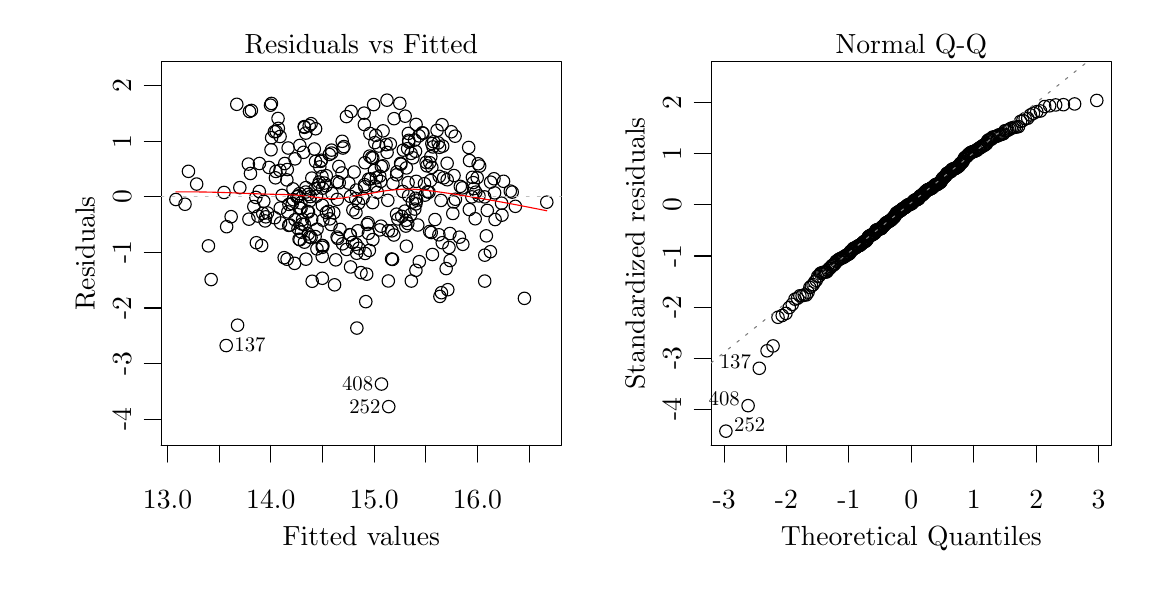
\begin{tikzpicture}[x=1pt,y=1pt]
\draw[color=white,opacity=0] (0,0) rectangle (397.48,198.74);
\begin{scope}
\path[clip] (  0.00,  0.00) rectangle (397.48,198.74);
\definecolor[named]{drawColor}{rgb}{0.75,0.39,0.77}
\definecolor[named]{drawColor}{rgb}{0.00,0.00,0.00}

\draw[color=drawColor,line cap=round,line join=round,fill opacity=0.00,] ( 50.35, 48.00) -- (180.98, 48.00);

\draw[color=drawColor,line cap=round,line join=round,fill opacity=0.00,] ( 50.35, 48.00) -- ( 50.35, 42.00);

\draw[color=drawColor,line cap=round,line join=round,fill opacity=0.00,] ( 69.01, 48.00) -- ( 69.01, 42.00);

\draw[color=drawColor,line cap=round,line join=round,fill opacity=0.00,] ( 87.67, 48.00) -- ( 87.67, 42.00);

\draw[color=drawColor,line cap=round,line join=round,fill opacity=0.00,] (106.33, 48.00) -- (106.33, 42.00);

\draw[color=drawColor,line cap=round,line join=round,fill opacity=0.00,] (125.00, 48.00) -- (125.00, 42.00);

\draw[color=drawColor,line cap=round,line join=round,fill opacity=0.00,] (143.66, 48.00) -- (143.66, 42.00);

\draw[color=drawColor,line cap=round,line join=round,fill opacity=0.00,] (162.32, 48.00) -- (162.32, 42.00);

\draw[color=drawColor,line cap=round,line join=round,fill opacity=0.00,] (180.98, 48.00) -- (180.98, 42.00);

\node[color=drawColor,anchor=base,inner sep=0pt, outer sep=0pt, scale=  1.00] at ( 50.35, 25.20) {13.0%
};

\node[color=drawColor,anchor=base,inner sep=0pt, outer sep=0pt, scale=  1.00] at ( 87.67, 25.20) {14.0%
};

\node[color=drawColor,anchor=base,inner sep=0pt, outer sep=0pt, scale=  1.00] at (125.00, 25.20) {15.0%
};

\node[color=drawColor,anchor=base,inner sep=0pt, outer sep=0pt, scale=  1.00] at (162.32, 25.20) {16.0%
};

\draw[color=drawColor,line cap=round,line join=round,fill opacity=0.00,] ( 48.00, 57.41) -- ( 48.00,178.06);

\draw[color=drawColor,line cap=round,line join=round,fill opacity=0.00,] ( 48.00, 57.41) -- ( 42.00, 57.41);

\draw[color=drawColor,line cap=round,line join=round,fill opacity=0.00,] ( 48.00, 77.52) -- ( 42.00, 77.52);

\draw[color=drawColor,line cap=round,line join=round,fill opacity=0.00,] ( 48.00, 97.63) -- ( 42.00, 97.63);

\draw[color=drawColor,line cap=round,line join=round,fill opacity=0.00,] ( 48.00,117.73) -- ( 42.00,117.73);

\draw[color=drawColor,line cap=round,line join=round,fill opacity=0.00,] ( 48.00,137.84) -- ( 42.00,137.84);

\draw[color=drawColor,line cap=round,line join=round,fill opacity=0.00,] ( 48.00,157.95) -- ( 42.00,157.95);

\draw[color=drawColor,line cap=round,line join=round,fill opacity=0.00,] ( 48.00,178.06) -- ( 42.00,178.06);

\node[rotate= 90.00,color=drawColor,anchor=base,inner sep=0pt, outer sep=0pt, scale=  1.00] at ( 37.20, 57.41) {-4%
};

\node[rotate= 90.00,color=drawColor,anchor=base,inner sep=0pt, outer sep=0pt, scale=  1.00] at ( 37.20, 77.52) {-3%
};

\node[rotate= 90.00,color=drawColor,anchor=base,inner sep=0pt, outer sep=0pt, scale=  1.00] at ( 37.20, 97.63) {-2%
};

\node[rotate= 90.00,color=drawColor,anchor=base,inner sep=0pt, outer sep=0pt, scale=  1.00] at ( 37.20,117.73) {-1%
};

\node[rotate= 90.00,color=drawColor,anchor=base,inner sep=0pt, outer sep=0pt, scale=  1.00] at ( 37.20,137.84) {0%
};

\node[rotate= 90.00,color=drawColor,anchor=base,inner sep=0pt, outer sep=0pt, scale=  1.00] at ( 37.20,157.95) {1%
};

\node[rotate= 90.00,color=drawColor,anchor=base,inner sep=0pt, outer sep=0pt, scale=  1.00] at ( 37.20,178.06) {2%
};

\draw[color=drawColor,line cap=round,line join=round,fill opacity=0.00,] ( 48.00, 48.00) --
	(192.74, 48.00) --
	(192.74,186.74) --
	( 48.00,186.74) --
	( 48.00, 48.00);
\end{scope}
\begin{scope}
\path[clip] (  0.00,  0.00) rectangle (198.74,198.74);
\definecolor[named]{drawColor}{rgb}{0.75,0.39,0.77}
\definecolor[named]{drawColor}{rgb}{0.00,0.00,0.00}

\node[color=drawColor,anchor=base,inner sep=0pt, outer sep=0pt, scale=  1.00] at (120.37, 12.00) {Fitted values%
};

\node[rotate= 90.00,color=drawColor,anchor=base,inner sep=0pt, outer sep=0pt, scale=  1.00] at ( 24.00,117.37) {Residuals%
};
\end{scope}
\begin{scope}
\path[clip] ( 48.00, 48.00) rectangle (192.74,186.74);
\definecolor[named]{drawColor}{rgb}{0.75,0.39,0.77}
\definecolor[named]{drawColor}{rgb}{0.00,0.00,0.00}

\draw[color=drawColor,line cap=round,line join=round,fill opacity=0.00,] (111.88,122.76) circle (  2.25);

\draw[color=drawColor,line cap=round,line join=round,fill opacity=0.00,] (149.15,136.51) circle (  2.25);

\draw[color=drawColor,line cap=round,line join=round,fill opacity=0.00,] (107.02,142.79) circle (  2.25);

\draw[color=drawColor,line cap=round,line join=round,fill opacity=0.00,] ( 98.18,133.75) circle (  2.25);

\draw[color=drawColor,line cap=round,line join=round,fill opacity=0.00,] (136.20,166.96) circle (  2.25);

\draw[color=drawColor,line cap=round,line join=round,fill opacity=0.00,] ( 92.70,149.85) circle (  2.25);

\draw[color=drawColor,line cap=round,line join=round,fill opacity=0.00,] (138.79,135.92) circle (  2.25);

\draw[color=drawColor,line cap=round,line join=round,fill opacity=0.00,] ( 98.68,125.06) circle (  2.25);

\draw[color=drawColor,line cap=round,line join=round,fill opacity=0.00,] (126.14,139.44) circle (  2.25);

\draw[color=drawColor,line cap=round,line join=round,fill opacity=0.00,] (106.36,140.94) circle (  2.25);

\draw[color=drawColor,line cap=round,line join=round,fill opacity=0.00,] (101.27,132.34) circle (  2.25);

\draw[color=drawColor,line cap=round,line join=round,fill opacity=0.00,] (159.46,150.93) circle (  2.25);

\draw[color=drawColor,line cap=round,line join=round,fill opacity=0.00,] (162.59,149.76) circle (  2.25);

\draw[color=drawColor,line cap=round,line join=round,fill opacity=0.00,] (161.51,129.89) circle (  2.25);

\draw[color=drawColor,line cap=round,line join=round,fill opacity=0.00,] ( 87.73,154.82) circle (  2.25);

\draw[color=drawColor,line cap=round,line join=round,fill opacity=0.00,] (111.61,123.29) circle (  2.25);

\draw[color=drawColor,line cap=round,line join=round,fill opacity=0.00,] (104.36,126.13) circle (  2.25);

\draw[color=drawColor,line cap=round,line join=round,fill opacity=0.00,] (104.93,142.23) circle (  2.25);

\draw[color=drawColor,line cap=round,line join=round,fill opacity=0.00,] (118.56,140.24) circle (  2.25);

\draw[color=drawColor,line cap=round,line join=round,fill opacity=0.00,] ( 90.96,147.40) circle (  2.25);

\draw[color=drawColor,line cap=round,line join=round,fill opacity=0.00,] ( 75.36,171.25) circle (  2.25);

\draw[color=drawColor,line cap=round,line join=round,fill opacity=0.00,] (102.22,164.24) circle (  2.25);

\draw[color=drawColor,line cap=round,line join=round,fill opacity=0.00,] (159.39,133.22) circle (  2.25);

\draw[color=drawColor,line cap=round,line join=round,fill opacity=0.00,] (122.91,124.60) circle (  2.25);

\draw[color=drawColor,line cap=round,line join=round,fill opacity=0.00,] (154.36,136.94) circle (  2.25);

\draw[color=drawColor,line cap=round,line join=round,fill opacity=0.00,] (103.83,162.41) circle (  2.25);

\draw[color=drawColor,line cap=round,line join=round,fill opacity=0.00,] (119.52,119.23) circle (  2.25);

\draw[color=drawColor,line cap=round,line join=round,fill opacity=0.00,] (103.70,140.82) circle (  2.25);

\draw[color=drawColor,line cap=round,line join=round,fill opacity=0.00,] (137.46,138.16) circle (  2.25);

\draw[color=drawColor,line cap=round,line join=round,fill opacity=0.00,] ( 97.12,137.83) circle (  2.25);

\draw[color=drawColor,line cap=round,line join=round,fill opacity=0.00,] (106.49,120.13) circle (  2.25);

\draw[color=drawColor,line cap=round,line join=round,fill opacity=0.00,] (128.23,149.03) circle (  2.25);

\draw[color=drawColor,line cap=round,line join=round,fill opacity=0.00,] (151.37,149.95) circle (  2.25);

\draw[color=drawColor,line cap=round,line join=round,fill opacity=0.00,] (101.69,123.31) circle (  2.25);

\draw[color=drawColor,line cap=round,line join=round,fill opacity=0.00,] (127.36,143.39) circle (  2.25);

\draw[color=drawColor,line cap=round,line join=round,fill opacity=0.00,] (145.07,125.30) circle (  2.25);

\draw[color=drawColor,line cap=round,line join=round,fill opacity=0.00,] (113.58,120.83) circle (  2.25);

\draw[color=drawColor,line cap=round,line join=round,fill opacity=0.00,] (171.04,135.52) circle (  2.25);

\draw[color=drawColor,line cap=round,line join=round,fill opacity=0.00,] (115.82,142.78) circle (  2.25);

\draw[color=drawColor,line cap=round,line join=round,fill opacity=0.00,] (149.77,156.15) circle (  2.25);

\draw[color=drawColor,line cap=round,line join=round,fill opacity=0.00,] (102.44,129.70) circle (  2.25);

\draw[color=drawColor,line cap=round,line join=round,fill opacity=0.00,] (145.85,157.05) circle (  2.25);

\draw[color=drawColor,line cap=round,line join=round,fill opacity=0.00,] (136.56,129.32) circle (  2.25);

\draw[color=drawColor,line cap=round,line join=round,fill opacity=0.00,] (149.31,103.18) circle (  2.25);

\draw[color=drawColor,line cap=round,line join=round,fill opacity=0.00,] ( 84.35,120.20) circle (  2.25);

\draw[color=drawColor,line cap=round,line join=round,fill opacity=0.00,] ( 98.12,156.38) circle (  2.25);

\draw[color=drawColor,line cap=round,line join=round,fill opacity=0.00,] (106.26,119.57) circle (  2.25);

\draw[color=drawColor,line cap=round,line join=round,fill opacity=0.00,] (154.25,159.73) circle (  2.25);

\draw[color=drawColor,line cap=round,line join=round,fill opacity=0.00,] (111.11,115.04) circle (  2.25);

\draw[color=drawColor,line cap=round,line join=round,fill opacity=0.00,] (143.76,150.28) circle (  2.25);

\draw[color=drawColor,line cap=round,line join=round,fill opacity=0.00,] (149.61,121.24) circle (  2.25);

\draw[color=drawColor,line cap=round,line join=round,fill opacity=0.00,] (130.12,107.41) circle (  2.25);

\draw[color=drawColor,line cap=round,line join=round,fill opacity=0.00,] (129.67,153.86) circle (  2.25);

\draw[color=drawColor,line cap=round,line join=round,fill opacity=0.00,] (162.86,138.14) circle (  2.25);

\draw[color=drawColor,line cap=round,line join=round,fill opacity=0.00,] (102.20,123.16) circle (  2.25);

\draw[color=drawColor,line cap=round,line join=round,fill opacity=0.00,] ( 99.78,127.81) circle (  2.25);

\draw[color=drawColor,line cap=round,line join=round,fill opacity=0.00,] ( 80.64,169.04) circle (  2.25);

\draw[color=drawColor,line cap=round,line join=round,fill opacity=0.00,] (106.47,129.38) circle (  2.25);

\draw[color=drawColor,line cap=round,line join=round,fill opacity=0.00,] (132.19,166.05) circle (  2.25);

\draw[color=drawColor,line cap=round,line join=round,fill opacity=0.00,] (118.45,120.66) circle (  2.25);

\draw[color=drawColor,line cap=round,line join=round,fill opacity=0.00,] (122.30,109.86) circle (  2.25);

\draw[color=drawColor,line cap=round,line join=round,fill opacity=0.00,] (151.61,104.26) circle (  2.25);

\draw[color=drawColor,line cap=round,line join=round,fill opacity=0.00,] ( 89.33,144.68) circle (  2.25);

\draw[color=drawColor,line cap=round,line join=round,fill opacity=0.00,] (131.64,115.19) circle (  2.25);

\draw[color=drawColor,line cap=round,line join=round,fill opacity=0.00,] ( 83.49,139.75) circle (  2.25);

\draw[color=drawColor,line cap=round,line join=round,fill opacity=0.00,] ( 85.11,136.20) circle (  2.25);

\draw[color=drawColor,line cap=round,line join=round,fill opacity=0.00,] (101.52,163.53) circle (  2.25);

\draw[color=drawColor,line cap=round,line join=round,fill opacity=0.00,] (139.67,133.40) circle (  2.25);

\draw[color=drawColor,line cap=round,line join=round,fill opacity=0.00,] ( 75.64, 91.43) circle (  2.25);

\draw[color=drawColor,line cap=round,line join=round,fill opacity=0.00,] ( 87.95,159.18) circle (  2.25);

\draw[color=drawColor,line cap=round,line join=round,fill opacity=0.00,] (129.31,156.67) circle (  2.25);

\draw[color=drawColor,line cap=round,line join=round,fill opacity=0.00,] ( 92.49,115.82) circle (  2.25);

\draw[color=drawColor,line cap=round,line join=round,fill opacity=0.00,] (152.04,119.51) circle (  2.25);

\draw[color=drawColor,line cap=round,line join=round,fill opacity=0.00,] (116.68,168.67) circle (  2.25);

\draw[color=drawColor,line cap=round,line join=round,fill opacity=0.00,] ( 89.50,146.99) circle (  2.25);

\draw[color=drawColor,line cap=round,line join=round,fill opacity=0.00,] (168.51,139.25) circle (  2.25);

\draw[color=drawColor,line cap=round,line join=round,fill opacity=0.00,] (111.67,143.29) circle (  2.25);

\draw[color=drawColor,line cap=round,line join=round,fill opacity=0.00,] ( 93.61,147.68) circle (  2.25);

\draw[color=drawColor,line cap=round,line join=round,fill opacity=0.00,] ( 98.02,138.96) circle (  2.25);

\draw[color=drawColor,line cap=round,line join=round,fill opacity=0.00,] (129.94,136.55) circle (  2.25);

\draw[color=drawColor,line cap=round,line join=round,fill opacity=0.00,] (153.86,145.50) circle (  2.25);

\draw[color=drawColor,line cap=round,line join=round,fill opacity=0.00,] (109.79,139.00) circle (  2.25);

\draw[color=drawColor,line cap=round,line join=round,fill opacity=0.00,] (156.87,141.04) circle (  2.25);

\draw[color=drawColor,line cap=round,line join=round,fill opacity=0.00,] ( 79.54,149.65) circle (  2.25);

\draw[color=drawColor,line cap=round,line join=round,fill opacity=0.00,] (103.83,150.62) circle (  2.25);

\draw[color=drawColor,line cap=round,line join=round,fill opacity=0.00,] ( 98.93,127.99) circle (  2.25);

\draw[color=drawColor,line cap=round,line join=round,fill opacity=0.00,] (100.30,139.55) circle (  2.25);

\draw[color=drawColor,line cap=round,line join=round,fill opacity=0.00,] (116.25,124.13) circle (  2.25);

\draw[color=drawColor,line cap=round,line join=round,fill opacity=0.00,] (144.80,139.49) circle (  2.25);

\draw[color=drawColor,line cap=round,line join=round,fill opacity=0.00,] (152.88,161.33) circle (  2.25);

\draw[color=drawColor,line cap=round,line join=round,fill opacity=0.00,] (123.47,160.70) circle (  2.25);

\draw[color=drawColor,line cap=round,line join=round,fill opacity=0.00,] (165.54,123.71) circle (  2.25);

\draw[color=drawColor,line cap=round,line join=round,fill opacity=0.00,] ( 96.41,129.50) circle (  2.25);

\draw[color=drawColor,line cap=round,line join=round,fill opacity=0.00,] (160.81,142.95) circle (  2.25);

\draw[color=drawColor,line cap=round,line join=round,fill opacity=0.00,] (102.48,144.58) circle (  2.25);

\draw[color=drawColor,line cap=round,line join=round,fill opacity=0.00,] (155.80,123.24) circle (  2.25);

\draw[color=drawColor,line cap=round,line join=round,fill opacity=0.00,] ( 93.81,132.37) circle (  2.25);

\draw[color=drawColor,line cap=round,line join=round,fill opacity=0.00,] (143.34,138.43) circle (  2.25);

\draw[color=drawColor,line cap=round,line join=round,fill opacity=0.00,] (117.19,121.31) circle (  2.25);

\draw[color=drawColor,line cap=round,line join=round,fill opacity=0.00,] ( 86.45,131.99) circle (  2.25);

\draw[color=drawColor,line cap=round,line join=round,fill opacity=0.00,] (105.16,143.14) circle (  2.25);

\draw[color=drawColor,line cap=round,line join=round,fill opacity=0.00,] (125.81,144.70) circle (  2.25);

\draw[color=drawColor,line cap=round,line join=round,fill opacity=0.00,] (133.10,131.55) circle (  2.25);

\draw[color=drawColor,line cap=round,line join=round,fill opacity=0.00,] (126.66,156.16) circle (  2.25);

\draw[color=drawColor,line cap=round,line join=round,fill opacity=0.00,] (114.07,155.97) circle (  2.25);

\draw[color=drawColor,line cap=round,line join=round,fill opacity=0.00,] (121.58,141.48) circle (  2.25);

\draw[color=drawColor,line cap=round,line join=round,fill opacity=0.00,] (132.12,124.02) circle (  2.25);

\draw[color=drawColor,line cap=round,line join=round,fill opacity=0.00,] ( 65.12,120.09) circle (  2.25);

\draw[color=drawColor,line cap=round,line join=round,fill opacity=0.00,] (148.40,124.10) circle (  2.25);

\draw[color=drawColor,line cap=round,line join=round,fill opacity=0.00,] (113.72,155.45) circle (  2.25);

\draw[color=drawColor,line cap=round,line join=round,fill opacity=0.00,] (142.65,160.78) circle (  2.25);

\draw[color=drawColor,line cap=round,line join=round,fill opacity=0.00,] (164.97,116.74) circle (  2.25);

\draw[color=drawColor,line cap=round,line join=round,fill opacity=0.00,] (171.75,143.43) circle (  2.25);

\draw[color=drawColor,line cap=round,line join=round,fill opacity=0.00,] (157.04,120.65) circle (  2.25);

\draw[color=drawColor,line cap=round,line join=round,fill opacity=0.00,] ( 71.53, 84.08) circle (  2.25);

\draw[color=drawColor,line cap=round,line join=round,fill opacity=0.00,] (101.97,137.89) circle (  2.25);

\draw[color=drawColor,line cap=round,line join=round,fill opacity=0.00,] ( 89.55,161.44) circle (  2.25);

\draw[color=drawColor,line cap=round,line join=round,fill opacity=0.00,] ( 82.27,137.61) circle (  2.25);

\draw[color=drawColor,line cap=round,line join=round,fill opacity=0.00,] (137.10,155.22) circle (  2.25);

\draw[color=drawColor,line cap=round,line join=round,fill opacity=0.00,] (125.57,160.02) circle (  2.25);

\draw[color=drawColor,line cap=round,line join=round,fill opacity=0.00,] (136.44,127.25) circle (  2.25);

\draw[color=drawColor,line cap=round,line join=round,fill opacity=0.00,] ( 99.71,163.18) circle (  2.25);

\draw[color=drawColor,line cap=round,line join=round,fill opacity=0.00,] ( 70.76,139.39) circle (  2.25);

\draw[color=drawColor,line cap=round,line join=round,fill opacity=0.00,] (161.00,140.79) circle (  2.25);

\draw[color=drawColor,line cap=round,line join=round,fill opacity=0.00,] ( 71.70,127.02) circle (  2.25);

\draw[color=drawColor,line cap=round,line join=round,fill opacity=0.00,] (115.02,118.81) circle (  2.25);

\draw[color=drawColor,line cap=round,line join=round,fill opacity=0.00,] (152.38,124.56) circle (  2.25);

\draw[color=drawColor,line cap=round,line join=round,fill opacity=0.00,] (105.69,150.63) circle (  2.25);

\draw[color=drawColor,line cap=round,line join=round,fill opacity=0.00,] ( 82.44,121.23) circle (  2.25);

\draw[color=drawColor,line cap=round,line join=round,fill opacity=0.00,] (106.29,134.75) circle (  2.25);

\draw[color=drawColor,line cap=round,line join=round,fill opacity=0.00,] ( 60.86,142.43) circle (  2.25);

\draw[color=drawColor,line cap=round,line join=round,fill opacity=0.00,] ( 57.90,147.03) circle (  2.25);

\draw[color=drawColor,line cap=round,line join=round,fill opacity=0.00,] (145.47,152.32) circle (  2.25);

\draw[color=drawColor,line cap=round,line join=round,fill opacity=0.00,] (122.49,127.84) circle (  2.25);

\draw[color=drawColor,line cap=round,line join=round,fill opacity=0.00,] (112.24,148.79) circle (  2.25);

\draw[color=drawColor,line cap=round,line join=round,fill opacity=0.00,] (135.55,154.70) circle (  2.25);

\draw[color=drawColor,line cap=round,line join=round,fill opacity=0.00,] (160.31,137.79) circle (  2.25);

\draw[color=drawColor,line cap=round,line join=round,fill opacity=0.00,] (123.71,144.28) circle (  2.25);

\draw[color=drawColor,line cap=round,line join=round,fill opacity=0.00,] (118.43,132.12) circle (  2.25);

\draw[color=drawColor,line cap=round,line join=round,fill opacity=0.00,] (144.29,139.66) circle (  2.25);

\draw[color=drawColor,line cap=round,line join=round,fill opacity=0.00,] ( 97.48,126.39) circle (  2.25);

\draw[color=drawColor,line cap=round,line join=round,fill opacity=0.00,] ( 83.54,149.86) circle (  2.25);

\draw[color=drawColor,line cap=round,line join=round,fill opacity=0.00,] (141.31,114.38) circle (  2.25);

\draw[color=drawColor,line cap=round,line join=round,fill opacity=0.00,] (108.94,129.85) circle (  2.25);

\draw[color=drawColor,line cap=round,line join=round,fill opacity=0.00,] (145.84,148.44) circle (  2.25);

\draw[color=drawColor,line cap=round,line join=round,fill opacity=0.00,] (121.73,117.36) circle (  2.25);

\draw[color=drawColor,line cap=round,line join=round,fill opacity=0.00,] (134.96,130.75) circle (  2.25);

\draw[color=drawColor,line cap=round,line join=round,fill opacity=0.00,] (144.05,149.03) circle (  2.25);

\draw[color=drawColor,line cap=round,line join=round,fill opacity=0.00,] (119.12,125.54) circle (  2.25);

\draw[color=drawColor,line cap=round,line join=round,fill opacity=0.00,] (111.68,136.90) circle (  2.25);

\draw[color=drawColor,line cap=round,line join=round,fill opacity=0.00,] (140.08,135.26) circle (  2.25);

\draw[color=drawColor,line cap=round,line join=round,fill opacity=0.00,] (120.98,137.33) circle (  2.25);

\draw[color=drawColor,line cap=round,line join=round,fill opacity=0.00,] (168.30,144.34) circle (  2.25);

\draw[color=drawColor,line cap=round,line join=round,fill opacity=0.00,] (121.46,163.95) circle (  2.25);

\draw[color=drawColor,line cap=round,line join=round,fill opacity=0.00,] (116.38,124.04) circle (  2.25);

\draw[color=drawColor,line cap=round,line join=round,fill opacity=0.00,] (118.75, 90.40) circle (  2.25);

\draw[color=drawColor,line cap=round,line join=round,fill opacity=0.00,] (124.46,135.72) circle (  2.25);

\draw[color=drawColor,line cap=round,line join=round,fill opacity=0.00,] (102.60,107.31) circle (  2.25);

\draw[color=drawColor,line cap=round,line join=round,fill opacity=0.00,] (112.67,126.04) circle (  2.25);

\draw[color=drawColor,line cap=round,line join=round,fill opacity=0.00,] ( 99.12,129.59) circle (  2.25);

\draw[color=drawColor,line cap=round,line join=round,fill opacity=0.00,] (162.22,144.74) circle (  2.25);

\draw[color=drawColor,line cap=round,line join=round,fill opacity=0.00,] (123.27,118.45) circle (  2.25);

\draw[color=drawColor,line cap=round,line join=round,fill opacity=0.00,] (117.31,133.08) circle (  2.25);

\draw[color=drawColor,line cap=round,line join=round,fill opacity=0.00,] (138.43,107.38) circle (  2.25);

\draw[color=drawColor,line cap=round,line join=round,fill opacity=0.00,] ( 76.47,141.15) circle (  2.25);

\draw[color=drawColor,line cap=round,line join=round,fill opacity=0.00,] (127.01,145.30) circle (  2.25);

\draw[color=drawColor,line cap=round,line join=round,fill opacity=0.00,] ( 85.58,129.11) circle (  2.25);

\draw[color=drawColor,line cap=round,line join=round,fill opacity=0.00,] (165.88,132.91) circle (  2.25);

\draw[color=drawColor,line cap=round,line join=round,fill opacity=0.00,] (187.38,135.89) circle (  2.25);

\draw[color=drawColor,line cap=round,line join=round,fill opacity=0.00,] ( 87.88,171.56) circle (  2.25);

\draw[color=drawColor,line cap=round,line join=round,fill opacity=0.00,] (128.21,161.65) circle (  2.25);

\draw[color=drawColor,line cap=round,line join=round,fill opacity=0.00,] ( 97.86,122.49) circle (  2.25);

\draw[color=drawColor,line cap=round,line join=round,fill opacity=0.00,] (160.50,144.86) circle (  2.25);

\draw[color=drawColor,line cap=round,line join=round,fill opacity=0.00,] (137.35,160.72) circle (  2.25);

\draw[color=drawColor,line cap=round,line join=round,fill opacity=0.00,] (124.51,151.82) circle (  2.25);

\draw[color=drawColor,line cap=round,line join=round,fill opacity=0.00,] (152.45,114.80) circle (  2.25);

\draw[color=drawColor,line cap=round,line join=round,fill opacity=0.00,] (121.98, 99.93) circle (  2.25);

\draw[color=drawColor,line cap=round,line join=round,fill opacity=0.00,] (145.62,124.91) circle (  2.25);

\draw[color=drawColor,line cap=round,line join=round,fill opacity=0.00,] ( 99.49,153.90) circle (  2.25);

\draw[color=drawColor,line cap=round,line join=round,fill opacity=0.00,] ( 93.45,143.93) circle (  2.25);

\draw[color=drawColor,line cap=round,line join=round,fill opacity=0.00,] ( 97.59,138.17) circle (  2.25);

\draw[color=drawColor,line cap=round,line join=round,fill opacity=0.00,] (148.64,155.71) circle (  2.25);

\draw[color=drawColor,line cap=round,line join=round,fill opacity=0.00,] (119.36,135.49) circle (  2.25);

\draw[color=drawColor,line cap=round,line join=round,fill opacity=0.00,] (103.37,155.10) circle (  2.25);

\draw[color=drawColor,line cap=round,line join=round,fill opacity=0.00,] (108.50,132.61) circle (  2.25);

\draw[color=drawColor,line cap=round,line join=round,fill opacity=0.00,] (100.33,115.29) circle (  2.25);

\draw[color=drawColor,line cap=round,line join=round,fill opacity=0.00,] (164.91,137.79) circle (  2.25);

\draw[color=drawColor,line cap=round,line join=round,fill opacity=0.00,] ( 87.55,170.93) circle (  2.25);

\draw[color=drawColor,line cap=round,line join=round,fill opacity=0.00,] (171.19,131.20) circle (  2.25);

\draw[color=drawColor,line cap=round,line join=round,fill opacity=0.00,] (142.39,160.96) circle (  2.25);

\draw[color=drawColor,line cap=round,line join=round,fill opacity=0.00,] ( 90.27,166.13) circle (  2.25);

\draw[color=drawColor,line cap=round,line join=round,fill opacity=0.00,] (125.12,147.33) circle (  2.25);

\draw[color=drawColor,line cap=round,line join=round,fill opacity=0.00,] (140.76,127.63) circle (  2.25);

\draw[color=drawColor,line cap=round,line join=round,fill opacity=0.00,] ( 98.51,135.61) circle (  2.25);

\draw[color=drawColor,line cap=round,line join=round,fill opacity=0.00,] (131.30,115.35) circle (  2.25);

\draw[color=drawColor,line cap=round,line join=round,fill opacity=0.00,] (168.70,129.61) circle (  2.25);

\draw[color=drawColor,line cap=round,line join=round,fill opacity=0.00,] (140.15,163.99) circle (  2.25);

\draw[color=drawColor,line cap=round,line join=round,fill opacity=0.00,] (179.30,101.13) circle (  2.25);

\draw[color=drawColor,line cap=round,line join=round,fill opacity=0.00,] (136.12,132.65) circle (  2.25);

\draw[color=drawColor,line cap=round,line join=round,fill opacity=0.00,] (130.08,125.57) circle (  2.25);

\draw[color=drawColor,line cap=round,line join=round,fill opacity=0.00,] (140.18,143.40) circle (  2.25);

\draw[color=drawColor,line cap=round,line join=round,fill opacity=0.00,] (130.27, 62.00) circle (  2.25);

\draw[color=drawColor,line cap=round,line join=round,fill opacity=0.00,] (146.49,157.71) circle (  2.25);

\draw[color=drawColor,line cap=round,line join=round,fill opacity=0.00,] (138.34,153.50) circle (  2.25);

\draw[color=drawColor,line cap=round,line join=round,fill opacity=0.00,] (105.94,151.03) circle (  2.25);

\draw[color=drawColor,line cap=round,line join=round,fill opacity=0.00,] (106.27,108.39) circle (  2.25);

\draw[color=drawColor,line cap=round,line join=round,fill opacity=0.00,] (109.58,154.69) circle (  2.25);

\draw[color=drawColor,line cap=round,line join=round,fill opacity=0.00,] (100.93,132.56) circle (  2.25);

\draw[color=drawColor,line cap=round,line join=round,fill opacity=0.00,] (140.35,136.61) circle (  2.25);

\draw[color=drawColor,line cap=round,line join=round,fill opacity=0.00,] ( 91.19,128.38) circle (  2.25);

\draw[color=drawColor,line cap=round,line join=round,fill opacity=0.00,] (120.24,110.43) circle (  2.25);

\draw[color=drawColor,line cap=round,line join=round,fill opacity=0.00,] (124.53,122.38) circle (  2.25);

\draw[color=drawColor,line cap=round,line join=round,fill opacity=0.00,] (134.27,171.62) circle (  2.25);

\draw[color=drawColor,line cap=round,line join=round,fill opacity=0.00,] ( 84.75,131.85) circle (  2.25);

\draw[color=drawColor,line cap=round,line join=round,fill opacity=0.00,] ( 79.75,129.74) circle (  2.25);

\draw[color=drawColor,line cap=round,line join=round,fill opacity=0.00,] (121.53,142.20) circle (  2.25);

\draw[color=drawColor,line cap=round,line join=round,fill opacity=0.00,] (145.36,143.68) circle (  2.25);

\draw[color=drawColor,line cap=round,line join=round,fill opacity=0.00,] (143.19,142.56) circle (  2.25);

\draw[color=drawColor,line cap=round,line join=round,fill opacity=0.00,] (137.50,157.67) circle (  2.25);

\draw[color=drawColor,line cap=round,line join=round,fill opacity=0.00,] (130.84,156.93) circle (  2.25);

\draw[color=drawColor,line cap=round,line join=round,fill opacity=0.00,] (134.55,149.91) circle (  2.25);

\draw[color=drawColor,line cap=round,line join=round,fill opacity=0.00,] ( 56.65,135.13) circle (  2.25);

\draw[color=drawColor,line cap=round,line join=round,fill opacity=0.00,] (107.69,145.44) circle (  2.25);

\draw[color=drawColor,line cap=round,line join=round,fill opacity=0.00,] (116.47,112.47) circle (  2.25);

\draw[color=drawColor,line cap=round,line join=round,fill opacity=0.00,] (139.95,154.27) circle (  2.25);

\draw[color=drawColor,line cap=round,line join=round,fill opacity=0.00,] ( 96.38,151.53) circle (  2.25);

\draw[color=drawColor,line cap=round,line join=round,fill opacity=0.00,] (167.08,143.12) circle (  2.25);

\draw[color=drawColor,line cap=round,line join=round,fill opacity=0.00,] (134.68,149.59) circle (  2.25);

\draw[color=drawColor,line cap=round,line join=round,fill opacity=0.00,] ( 85.83,130.58) circle (  2.25);

\draw[color=drawColor,line cap=round,line join=round,fill opacity=0.00,] (159.16,155.65) circle (  2.25);

\draw[color=drawColor,line cap=round,line join=round,fill opacity=0.00,] ( 81.52,134.30) circle (  2.25);

\draw[color=drawColor,line cap=round,line join=round,fill opacity=0.00,] (146.25,155.85) circle (  2.25);

\draw[color=drawColor,line cap=round,line join=round,fill opacity=0.00,] (150.10,144.68) circle (  2.25);

\draw[color=drawColor,line cap=round,line join=round,fill opacity=0.00,] ( 95.40,135.34) circle (  2.25);

\draw[color=drawColor,line cap=round,line join=round,fill opacity=0.00,] (149.53,163.87) circle (  2.25);

\draw[color=drawColor,line cap=round,line join=round,fill opacity=0.00,] (129.64,172.74) circle (  2.25);

\draw[color=drawColor,line cap=round,line join=round,fill opacity=0.00,] (125.30,141.73) circle (  2.25);

\draw[color=drawColor,line cap=round,line join=round,fill opacity=0.00,] (109.63,153.63) circle (  2.25);

\draw[color=drawColor,line cap=round,line join=round,fill opacity=0.00,] (100.34,141.14) circle (  2.25);

\draw[color=drawColor,line cap=round,line join=round,fill opacity=0.00,] (118.33,137.17) circle (  2.25);

\draw[color=drawColor,line cap=round,line join=round,fill opacity=0.00,] (137.48,158.24) circle (  2.25);

\draw[color=drawColor,line cap=round,line join=round,fill opacity=0.00,] (174.88,139.52) circle (  2.25);

\draw[color=drawColor,line cap=round,line join=round,fill opacity=0.00,] ( 80.31,146.25) circle (  2.25);

\draw[color=drawColor,line cap=round,line join=round,fill opacity=0.00,] (107.74,132.11) circle (  2.25);

\draw[color=drawColor,line cap=round,line join=round,fill opacity=0.00,] (139.97,137.29) circle (  2.25);

\draw[color=drawColor,line cap=round,line join=round,fill opacity=0.00,] ( 99.82,162.93) circle (  2.25);

\draw[color=drawColor,line cap=round,line join=round,fill opacity=0.00,] (101.15,124.41) circle (  2.25);

\draw[color=drawColor,line cap=round,line join=round,fill opacity=0.00,] (147.73,161.81) circle (  2.25);

\draw[color=drawColor,line cap=round,line join=round,fill opacity=0.00,] (100.28,160.85) circle (  2.25);

\draw[color=drawColor,line cap=round,line join=round,fill opacity=0.00,] (127.59,148.76) circle (  2.25);

\draw[color=drawColor,line cap=round,line join=round,fill opacity=0.00,] ( 89.04,130.25) circle (  2.25);

\draw[color=drawColor,line cap=round,line join=round,fill opacity=0.00,] ( 96.26,113.78) circle (  2.25);

\draw[color=drawColor,line cap=round,line join=round,fill opacity=0.00,] ( 94.21,135.10) circle (  2.25);

\draw[color=drawColor,line cap=round,line join=round,fill opacity=0.00,] (145.09,150.14) circle (  2.25);

\draw[color=drawColor,line cap=round,line join=round,fill opacity=0.00,] ( 91.07,133.75) circle (  2.25);

\draw[color=drawColor,line cap=round,line join=round,fill opacity=0.00,] (124.11,152.04) circle (  2.25);

\draw[color=drawColor,line cap=round,line join=round,fill opacity=0.00,] (136.64,119.98) circle (  2.25);

\draw[color=drawColor,line cap=round,line join=round,fill opacity=0.00,] (148.14,157.31) circle (  2.25);

\draw[color=drawColor,line cap=round,line join=round,fill opacity=0.00,] (124.82,171.14) circle (  2.25);

\draw[color=drawColor,line cap=round,line join=round,fill opacity=0.00,] (106.14,145.17) circle (  2.25);

\draw[color=drawColor,line cap=round,line join=round,fill opacity=0.00,] (121.37,168.06) circle (  2.25);

\draw[color=drawColor,line cap=round,line join=round,fill opacity=0.00,] (125.24,157.39) circle (  2.25);

\draw[color=drawColor,line cap=round,line join=round,fill opacity=0.00,] (113.45,157.88) circle (  2.25);

\draw[color=drawColor,line cap=round,line join=round,fill opacity=0.00,] ( 88.94,161.33) circle (  2.25);

\draw[color=drawColor,line cap=round,line join=round,fill opacity=0.00,] (104.19,138.05) circle (  2.25);

\draw[color=drawColor,line cap=round,line join=round,fill opacity=0.00,] (164.95,107.37) circle (  2.25);

\draw[color=drawColor,line cap=round,line join=round,fill opacity=0.00,] (153.42,131.80) circle (  2.25);

\draw[color=drawColor,line cap=round,line join=round,fill opacity=0.00,] (146.98,129.61) circle (  2.25);

\draw[color=drawColor,line cap=round,line join=round,fill opacity=0.00,] (122.85,128.45) circle (  2.25);

\draw[color=drawColor,line cap=round,line join=round,fill opacity=0.00,] (153.74,135.96) circle (  2.25);

\draw[color=drawColor,line cap=round,line join=round,fill opacity=0.00,] ( 93.92,155.46) circle (  2.25);

\draw[color=drawColor,line cap=round,line join=round,fill opacity=0.00,] (138.22,131.41) circle (  2.25);

\draw[color=drawColor,line cap=round,line join=round,fill opacity=0.00,] (133.57,129.82) circle (  2.25);

\draw[color=drawColor,line cap=round,line join=round,fill opacity=0.00,] (113.38,146.43) circle (  2.25);

\draw[color=drawColor,line cap=round,line join=round,fill opacity=0.00,] (114.99,166.81) circle (  2.25);

\draw[color=drawColor,line cap=round,line join=round,fill opacity=0.00,] (148.76,101.82) circle (  2.25);

\draw[color=drawColor,line cap=round,line join=round,fill opacity=0.00,] ( 95.81,136.78) circle (  2.25);

\draw[color=drawColor,line cap=round,line join=round,fill opacity=0.00,] ( 98.56,133.64) circle (  2.25);

\draw[color=drawColor,line cap=round,line join=round,fill opacity=0.00,] (176.02,134.38) circle (  2.25);

\draw[color=drawColor,line cap=round,line join=round,fill opacity=0.00,] (121.67,150.13) circle (  2.25);

\draw[color=drawColor,line cap=round,line join=round,fill opacity=0.00,] (108.79,153.11) circle (  2.25);

\draw[color=drawColor,line cap=round,line join=round,fill opacity=0.00,] (110.41,132.05) circle (  2.25);

\draw[color=drawColor,line cap=round,line join=round,fill opacity=0.00,] (106.23,116.27) circle (  2.25);

\draw[color=drawColor,line cap=round,line join=round,fill opacity=0.00,] ( 91.01,159.62) circle (  2.25);

\draw[color=drawColor,line cap=round,line join=round,fill opacity=0.00,] (139.63,158.31) circle (  2.25);

\draw[color=drawColor,line cap=round,line join=round,fill opacity=0.00,] (141.20,159.84) circle (  2.25);

\draw[color=drawColor,line cap=round,line join=round,fill opacity=0.00,] (151.01,111.89) circle (  2.25);

\draw[color=drawColor,line cap=round,line join=round,fill opacity=0.00,] ( 93.53,115.26) circle (  2.25);

\draw[color=drawColor,line cap=round,line join=round,fill opacity=0.00,] ( 82.99,130.87) circle (  2.25);

\draw[color=drawColor,line cap=round,line join=round,fill opacity=0.00,] ( 91.73,138.33) circle (  2.25);

\draw[color=drawColor,line cap=round,line join=round,fill opacity=0.00,] (107.60,141.82) circle (  2.25);

\draw[color=drawColor,line cap=round,line join=round,fill opacity=0.00,] (139.00,151.91) circle (  2.25);

\draw[color=drawColor,line cap=round,line join=round,fill opacity=0.00,] (135.37,139.74) circle (  2.25);

\draw[color=drawColor,line cap=round,line join=round,fill opacity=0.00,] (146.06,116.97) circle (  2.25);

\draw[color=drawColor,line cap=round,line join=round,fill opacity=0.00,] (127.00,125.86) circle (  2.25);

\draw[color=drawColor,line cap=round,line join=round,fill opacity=0.00,] (110.69,106.01) circle (  2.25);

\draw[color=drawColor,line cap=round,line join=round,fill opacity=0.00,] (117.76,146.78) circle (  2.25);

\draw[color=drawColor,line cap=round,line join=round,fill opacity=0.00,] (151.39,143.99) circle (  2.25);

\draw[color=drawColor,line cap=round,line join=round,fill opacity=0.00,] (103.67,123.46) circle (  2.25);

\draw[color=drawColor,line cap=round,line join=round,fill opacity=0.00,] (133.13,145.78) circle (  2.25);

\draw[color=drawColor,line cap=round,line join=round,fill opacity=0.00,] ( 73.32,130.63) circle (  2.25);

\draw[color=drawColor,line cap=round,line join=round,fill opacity=0.00,] (133.21,146.81) circle (  2.25);

\draw[color=drawColor,line cap=round,line join=round,fill opacity=0.00,] (123.38,152.54) circle (  2.25);

\draw[color=drawColor,line cap=round,line join=round,fill opacity=0.00,] ( 79.95,168.65) circle (  2.25);

\draw[color=drawColor,line cap=round,line join=round,fill opacity=0.00,] (163.14,148.95) circle (  2.25);

\draw[color=drawColor,line cap=round,line join=round,fill opacity=0.00,] (104.33,119.00) circle (  2.25);

\draw[color=drawColor,line cap=round,line join=round,fill opacity=0.00,] (140.09,111.27) circle (  2.25);

\draw[color=drawColor,line cap=round,line join=round,fill opacity=0.00,] (161.72,139.51) circle (  2.25);

\draw[color=drawColor,line cap=round,line join=round,fill opacity=0.00,] (137.25,142.95) circle (  2.25);

\draw[color=drawColor,line cap=round,line join=round,fill opacity=0.00,] ( 90.37,162.56) circle (  2.25);

\draw[color=drawColor,line cap=round,line join=round,fill opacity=0.00,] (112.38,142.91) circle (  2.25);

\draw[color=drawColor,line cap=round,line join=round,fill opacity=0.00,] (118.69,117.43) circle (  2.25);

\draw[color=drawColor,line cap=round,line join=round,fill opacity=0.00,] (137.15,128.18) circle (  2.25);

\draw[color=drawColor,line cap=round,line join=round,fill opacity=0.00,] ( 94.58,127.63) circle (  2.25);

\draw[color=drawColor,line cap=round,line join=round,fill opacity=0.00,] ( 98.20,122.31) circle (  2.25);

\draw[color=drawColor,line cap=round,line join=round,fill opacity=0.00,] (167.01,118.00) circle (  2.25);

\draw[color=drawColor,line cap=round,line join=round,fill opacity=0.00,] (156.14,141.59) circle (  2.25);

\draw[color=drawColor,line cap=round,line join=round,fill opacity=0.00,] (123.01,144.21) circle (  2.25);

\draw[color=drawColor,line cap=round,line join=round,fill opacity=0.00,] ( 53.36,136.85) circle (  2.25);

\draw[color=drawColor,line cap=round,line join=round,fill opacity=0.00,] (105.35,148.62) circle (  2.25);

\draw[color=drawColor,line cap=round,line join=round,fill opacity=0.00,] ( 66.09,107.92) circle (  2.25);

\draw[color=drawColor,line cap=round,line join=round,fill opacity=0.00,] (174.19,139.89) circle (  2.25);

\draw[color=drawColor,line cap=round,line join=round,fill opacity=0.00,] (109.43,127.79) circle (  2.25);

\draw[color=drawColor,line cap=round,line join=round,fill opacity=0.00,] ( 99.81,121.44) circle (  2.25);

\draw[color=drawColor,line cap=round,line join=round,fill opacity=0.00,] (131.78,142.62) circle (  2.25);

\draw[color=drawColor,line cap=round,line join=round,fill opacity=0.00,] (148.52,145.22) circle (  2.25);

\draw[color=drawColor,line cap=round,line join=round,fill opacity=0.00,] (136.65,148.26) circle (  2.25);

\draw[color=drawColor,line cap=round,line join=round,fill opacity=0.00,] (127.65, 70.17) circle (  2.25);

\draw[color=drawColor,line cap=round,line join=round,fill opacity=0.00,] (101.76,136.36) circle (  2.25);

\draw[color=drawColor,line cap=round,line join=round,fill opacity=0.00,] ( 94.14,127.50) circle (  2.25);

\draw[color=drawColor,line cap=round,line join=round,fill opacity=0.00,] (127.48,127.22) circle (  2.25);

\draw[color=drawColor,line cap=round,line join=round,fill opacity=0.00,] (101.17,138.68) circle (  2.25);

\draw[color=drawColor,line cap=round,line join=round,fill opacity=0.00,] (116.44,137.95) circle (  2.25);

\draw[color=drawColor,line cap=round,line join=round,fill opacity=0.00,] ( 87.00,148.43) circle (  2.25);

\draw[color=drawColor,line cap=round,line join=round,fill opacity=0.00,] ( 95.68,140.67) circle (  2.25);

\draw[color=drawColor,line cap=round,line join=round,fill opacity=0.00,] (106.26,120.23) circle (  2.25);

\draw[color=drawColor,line cap=round,line join=round,fill opacity=0.00,] (131.41,125.54) circle (  2.25);
\definecolor[named]{drawColor}{rgb}{1.00,0.00,0.00}

\draw[color=drawColor,line cap=round,line join=round,fill opacity=0.00,] ( 53.36,139.62) --
	( 56.65,139.62) --
	( 57.90,139.61) --
	( 60.86,139.59) --
	( 65.12,139.53) --
	( 66.09,139.50) --
	( 70.76,139.37) --
	( 71.53,139.34) --
	( 71.70,139.34) --
	( 73.32,139.28) --
	( 75.36,139.20) --
	( 75.64,139.19) --
	( 76.47,139.15) --
	( 79.54,139.03) --
	( 79.75,139.02) --
	( 79.95,139.01) --
	( 80.31,139.00) --
	( 80.64,138.99) --
	( 81.52,138.95) --
	( 82.27,138.92) --
	( 82.44,138.92) --
	( 82.99,138.90) --
	( 83.49,138.88) --
	( 83.54,138.88) --
	( 84.35,138.85) --
	( 84.75,138.84) --
	( 85.11,138.83) --
	( 85.58,138.81) --
	( 85.83,138.81) --
	( 86.45,138.79) --
	( 87.00,138.77) --
	( 87.55,138.76) --
	( 87.73,138.75) --
	( 87.88,138.75) --
	( 87.95,138.75) --
	( 88.94,138.72) --
	( 89.04,138.72) --
	( 89.33,138.72) --
	( 89.50,138.71) --
	( 89.55,138.71) --
	( 90.27,138.70) --
	( 90.37,138.69) --
	( 90.96,138.68) --
	( 91.01,138.68) --
	( 91.07,138.68) --
	( 91.19,138.67) --
	( 91.73,138.66) --
	( 92.49,138.64) --
	( 92.70,138.64) --
	( 93.45,138.61) --
	( 93.53,138.61) --
	( 93.61,138.61) --
	( 93.81,138.60) --
	( 93.92,138.59) --
	( 94.14,138.58) --
	( 94.21,138.58) --
	( 94.58,138.56) --
	( 95.40,138.51) --
	( 95.68,138.50) --
	( 95.81,138.49) --
	( 96.26,138.46) --
	( 96.38,138.45) --
	( 96.41,138.45) --
	( 97.12,138.40) --
	( 97.48,138.37) --
	( 97.59,138.36) --
	( 97.86,138.33) --
	( 98.02,138.32) --
	( 98.12,138.31) --
	( 98.18,138.31) --
	( 98.20,138.30) --
	( 98.51,138.27) --
	( 98.56,138.27) --
	( 98.68,138.26) --
	( 98.93,138.23) --
	( 99.12,138.21) --
	( 99.49,138.17) --
	( 99.71,138.14) --
	( 99.78,138.14) --
	( 99.81,138.13) --
	( 99.82,138.13) --
	(100.28,138.08) --
	(100.30,138.07) --
	(100.33,138.07) --
	(100.34,138.07) --
	(100.93,138.00) --
	(101.15,137.98) --
	(101.17,137.98) --
	(101.27,137.96) --
	(101.52,137.94) --
	(101.69,137.91) --
	(101.76,137.90) --
	(101.97,137.88) --
	(102.20,137.85) --
	(102.22,137.84) --
	(102.44,137.81) --
	(102.48,137.81) --
	(102.60,137.79) --
	(103.37,137.70) --
	(103.67,137.66) --
	(103.70,137.65) --
	(103.83,137.64) --
	(103.83,137.64) --
	(104.19,137.59) --
	(104.33,137.58) --
	(104.36,137.57) --
	(104.93,137.50) --
	(105.16,137.48) --
	(105.35,137.46) --
	(105.69,137.43) --
	(105.94,137.41) --
	(106.14,137.39) --
	(106.23,137.38) --
	(106.26,137.38) --
	(106.26,137.38) --
	(106.27,137.38) --
	(106.29,137.37) --
	(106.36,137.37) --
	(106.47,137.36) --
	(106.49,137.36) --
	(107.02,137.30) --
	(107.60,137.25) --
	(107.69,137.24) --
	(107.74,137.23) --
	(108.50,137.18) --
	(108.79,137.16) --
	(108.94,137.15) --
	(109.43,137.16) --
	(109.58,137.16) --
	(109.63,137.16) --
	(109.79,137.17) --
	(110.41,137.18) --
	(110.69,137.18) --
	(111.11,137.19) --
	(111.61,137.23) --
	(111.67,137.23) --
	(111.68,137.23) --
	(111.88,137.25) --
	(112.24,137.28) --
	(112.38,137.29) --
	(112.67,137.31) --
	(113.38,137.35) --
	(113.45,137.36) --
	(113.58,137.37) --
	(113.72,137.39) --
	(114.07,137.44) --
	(114.99,137.62) --
	(115.02,137.63) --
	(115.82,137.76) --
	(116.25,137.83) --
	(116.38,137.85) --
	(116.44,137.86) --
	(116.47,137.87) --
	(116.68,137.90) --
	(117.19,137.99) --
	(117.31,138.01) --
	(117.76,138.09) --
	(118.33,138.18) --
	(118.43,138.20) --
	(118.45,138.20) --
	(118.56,138.22) --
	(118.69,138.24) --
	(118.75,138.24) --
	(119.12,138.30) --
	(119.36,138.33) --
	(119.52,138.35) --
	(120.24,138.48) --
	(120.98,138.61) --
	(121.37,138.68) --
	(121.46,138.69) --
	(121.53,138.71) --
	(121.58,138.71) --
	(121.67,138.73) --
	(121.73,138.74) --
	(121.98,138.78) --
	(122.30,138.82) --
	(122.49,138.85) --
	(122.85,138.91) --
	(122.91,138.92) --
	(123.01,138.94) --
	(123.27,138.98) --
	(123.38,139.00) --
	(123.47,139.02) --
	(123.71,139.06) --
	(124.11,139.13) --
	(124.46,139.20) --
	(124.51,139.21) --
	(124.53,139.21) --
	(124.82,139.27) --
	(125.12,139.32) --
	(125.24,139.35) --
	(125.30,139.36) --
	(125.57,139.41) --
	(125.81,139.46) --
	(126.14,139.52) --
	(126.66,139.61) --
	(127.00,139.67) --
	(127.01,139.68) --
	(127.36,139.74) --
	(127.48,139.76) --
	(127.59,139.78) --
	(127.65,139.79) --
	(128.21,139.87) --
	(128.23,139.87) --
	(129.31,140.02) --
	(129.64,140.07) --
	(129.67,140.07) --
	(129.94,140.10) --
	(130.08,140.12) --
	(130.12,140.13) --
	(130.27,140.15) --
	(130.84,140.21) --
	(131.30,140.26) --
	(131.41,140.27) --
	(131.64,140.29) --
	(131.78,140.31) --
	(132.12,140.34) --
	(132.19,140.35) --
	(133.10,140.41) --
	(133.13,140.42) --
	(133.21,140.42) --
	(133.57,140.45) --
	(134.27,140.51) --
	(134.55,140.54) --
	(134.68,140.54) --
	(134.96,140.55) --
	(135.37,140.56) --
	(135.55,140.57) --
	(136.12,140.58) --
	(136.20,140.59) --
	(136.44,140.59) --
	(136.56,140.59) --
	(136.64,140.60) --
	(136.65,140.60) --
	(137.10,140.58) --
	(137.15,140.58) --
	(137.25,140.58) --
	(137.35,140.57) --
	(137.46,140.57) --
	(137.48,140.57) --
	(137.50,140.57) --
	(138.22,140.57) --
	(138.34,140.58) --
	(138.43,140.58) --
	(138.79,140.58) --
	(139.00,140.57) --
	(139.63,140.53) --
	(139.67,140.53) --
	(139.95,140.51) --
	(139.97,140.51) --
	(140.08,140.50) --
	(140.09,140.50) --
	(140.15,140.50) --
	(140.18,140.50) --
	(140.35,140.49) --
	(140.76,140.46) --
	(141.20,140.43) --
	(141.31,140.42) --
	(142.39,140.31) --
	(142.65,140.28) --
	(143.19,140.23) --
	(143.34,140.21) --
	(143.76,140.16) --
	(144.05,140.13) --
	(144.29,140.10) --
	(144.80,140.04) --
	(145.07,140.01) --
	(145.09,140.01) --
	(145.36,139.98) --
	(145.47,139.96) --
	(145.62,139.95) --
	(145.84,139.92) --
	(145.85,139.92) --
	(146.06,139.89) --
	(146.25,139.87) --
	(146.49,139.84) --
	(146.98,139.77) --
	(147.73,139.68) --
	(148.14,139.62) --
	(148.40,139.58) --
	(148.52,139.57) --
	(148.64,139.55) --
	(148.76,139.54) --
	(149.15,139.48) --
	(149.31,139.46) --
	(149.53,139.43) --
	(149.61,139.42) --
	(149.77,139.39) --
	(150.10,139.35) --
	(151.01,139.21) --
	(151.37,139.16) --
	(151.39,139.16) --
	(151.61,139.13) --
	(152.04,139.06) --
	(152.38,139.01) --
	(152.45,139.00) --
	(152.88,138.94) --
	(153.42,138.85) --
	(153.74,138.81) --
	(153.86,138.79) --
	(154.25,138.73) --
	(154.36,138.71) --
	(155.80,138.49) --
	(156.14,138.43) --
	(156.87,138.32) --
	(157.04,138.29) --
	(159.16,137.95) --
	(159.39,137.92) --
	(159.46,137.90) --
	(160.31,137.77) --
	(160.50,137.73) --
	(160.81,137.68) --
	(161.00,137.65) --
	(161.51,137.57) --
	(161.72,137.53) --
	(162.22,137.45) --
	(162.59,137.39) --
	(162.86,137.34) --
	(163.14,137.30) --
	(164.91,137.00) --
	(164.95,136.99) --
	(164.97,136.99) --
	(165.54,136.89) --
	(165.88,136.83) --
	(167.01,136.63) --
	(167.08,136.62) --
	(168.30,136.41) --
	(168.51,136.37) --
	(168.70,136.34) --
	(171.04,135.92) --
	(171.19,135.89) --
	(171.75,135.79) --
	(174.19,135.34) --
	(174.88,135.21) --
	(176.02,135.00) --
	(179.30,134.37) --
	(187.38,132.78);
\end{scope}
\begin{scope}
\path[clip] (  0.00,  0.00) rectangle (397.48,198.74);
\definecolor[named]{drawColor}{rgb}{0.75,0.39,0.77}
\definecolor[named]{drawColor}{rgb}{0.00,0.00,0.00}

\node[color=drawColor,anchor=base,inner sep=0pt, outer sep=0pt, scale=  1.00] at (120.37,189.74) {Residuals vs Fitted%
};
\end{scope}
\begin{scope}
\path[clip] (  0.00,  0.00) rectangle (198.74,198.74);
\definecolor[named]{drawColor}{rgb}{0.75,0.39,0.77}
\definecolor[named]{drawColor}{rgb}{0.00,0.00,0.00}

\node[color=drawColor,anchor=base east,inner sep=0pt, outer sep=0pt, scale=  0.75] at (127.27, 59.70) {252%
};

\node[color=drawColor,anchor=base east,inner sep=0pt, outer sep=0pt, scale=  0.75] at (124.65, 67.87) {408%
};

\node[color=drawColor,anchor=base west,inner sep=0pt, outer sep=0pt, scale=  0.75] at ( 74.53, 81.78) {137%
};
\end{scope}
\begin{scope}
\path[clip] ( 48.00, 48.00) rectangle (192.74,186.74);
\definecolor[named]{drawColor}{rgb}{0.75,0.39,0.77}
\definecolor[named]{drawColor}{rgb}{0.75,0.75,0.75}

\draw[color=drawColor,dash pattern=on 1pt off 3pt ,line cap=round,line join=round,fill opacity=0.00,] ( 48.00,137.84) -- (192.74,137.84);
\end{scope}
\begin{scope}
\path[clip] (246.74, 48.00) rectangle (391.48,186.74);
\definecolor[named]{drawColor}{rgb}{0.75,0.39,0.77}
\end{scope}
\begin{scope}
\path[clip] (246.74, 48.00) rectangle (391.48,186.74);
\definecolor[named]{drawColor}{rgb}{0.75,0.39,0.77}
\definecolor[named]{drawColor}{rgb}{0.00,0.00,0.00}

\draw[color=drawColor,line cap=round,line join=round,fill opacity=0.00,] (297.91,118.74) circle (  2.25);

\draw[color=drawColor,line cap=round,line join=round,fill opacity=0.00,] (315.92,133.49) circle (  2.25);

\draw[color=drawColor,line cap=round,line join=round,fill opacity=0.00,] (325.40,140.43) circle (  2.25);

\draw[color=drawColor,line cap=round,line join=round,fill opacity=0.00,] (313.00,130.50) circle (  2.25);

\draw[color=drawColor,line cap=round,line join=round,fill opacity=0.00,] (361.16,166.21) circle (  2.25);

\draw[color=drawColor,line cap=round,line join=round,fill opacity=0.00,] (334.48,147.89) circle (  2.25);

\draw[color=drawColor,line cap=round,line join=round,fill opacity=0.00,] (315.24,132.86) circle (  2.25);

\draw[color=drawColor,line cap=round,line join=round,fill opacity=0.00,] (301.55,121.12) circle (  2.25);

\draw[color=drawColor,line cap=round,line join=round,fill opacity=0.00,] (320.46,136.68) circle (  2.25);

\draw[color=drawColor,line cap=round,line join=round,fill opacity=0.00,] (322.65,138.29) circle (  2.25);

\draw[color=drawColor,line cap=round,line join=round,fill opacity=0.00,] (311.06,129.02) circle (  2.25);

\draw[color=drawColor,line cap=round,line join=round,fill opacity=0.00,] (336.22,148.97) circle (  2.25);

\draw[color=drawColor,line cap=round,line join=round,fill opacity=0.00,] (333.86,147.78) circle (  2.25);

\draw[color=drawColor,line cap=round,line join=round,fill opacity=0.00,] (308.31,126.35) circle (  2.25);

\draw[color=drawColor,line cap=round,line join=round,fill opacity=0.00,] (341.94,154.25) circle (  2.25);

\draw[color=drawColor,line cap=round,line join=round,fill opacity=0.00,] (298.93,119.36) circle (  2.25);

\draw[color=drawColor,line cap=round,line join=round,fill opacity=0.00,] (303.10,122.35) circle (  2.25);

\draw[color=drawColor,line cap=round,line join=round,fill opacity=0.00,] (324.19,139.61) circle (  2.25);

\draw[color=drawColor,line cap=round,line join=round,fill opacity=0.00,] (321.97,137.50) circle (  2.25);

\draw[color=drawColor,line cap=round,line join=round,fill opacity=0.00,] (331.44,145.34) circle (  2.25);

\draw[color=drawColor,line cap=round,line join=round,fill opacity=0.00,] (371.26,171.02) circle (  2.25);

\draw[color=drawColor,line cap=round,line join=round,fill opacity=0.00,] (357.83,163.19) circle (  2.25);

\draw[color=drawColor,line cap=round,line join=round,fill opacity=0.00,] (312.30,129.89) circle (  2.25);

\draw[color=drawColor,line cap=round,line join=round,fill opacity=0.00,] (301.09,120.76) circle (  2.25);

\draw[color=drawColor,line cap=round,line join=round,fill opacity=0.00,] (316.93,133.95) circle (  2.25);

\draw[color=drawColor,line cap=round,line join=round,fill opacity=0.00,] (353.48,161.71) circle (  2.25);

\draw[color=drawColor,line cap=round,line join=round,fill opacity=0.00,] (292.63,114.96) circle (  2.25);

\draw[color=drawColor,line cap=round,line join=round,fill opacity=0.00,] (322.48,138.11) circle (  2.25);

\draw[color=drawColor,line cap=round,line join=round,fill opacity=0.00,] (318.95,135.26) circle (  2.25);

\draw[color=drawColor,line cap=round,line join=round,fill opacity=0.00,] (318.11,134.90) circle (  2.25);

\draw[color=drawColor,line cap=round,line join=round,fill opacity=0.00,] (293.93,115.74) circle (  2.25);

\draw[color=drawColor,line cap=round,line join=round,fill opacity=0.00,] (333.03,146.87) circle (  2.25);

\draw[color=drawColor,line cap=round,line join=round,fill opacity=0.00,] (334.70,147.91) circle (  2.25);

\draw[color=drawColor,line cap=round,line join=round,fill opacity=0.00,] (298.43,119.23) circle (  2.25);

\draw[color=drawColor,line cap=round,line join=round,fill opacity=0.00,] (326.10,140.85) circle (  2.25);

\draw[color=drawColor,line cap=round,line join=round,fill opacity=0.00,] (301.78,121.39) circle (  2.25);

\draw[color=drawColor,line cap=round,line join=round,fill opacity=0.00,] (295.72,116.72) circle (  2.25);

\draw[color=drawColor,line cap=round,line join=round,fill opacity=0.00,] (314.38,132.34) circle (  2.25);

\draw[color=drawColor,line cap=round,line join=round,fill opacity=0.00,] (324.88,140.27) circle (  2.25);

\draw[color=drawColor,line cap=round,line join=round,fill opacity=0.00,] (342.50,154.55) circle (  2.25);

\draw[color=drawColor,line cap=round,line join=round,fill opacity=0.00,] (307.56,126.20) circle (  2.25);

\draw[color=drawColor,line cap=round,line join=round,fill opacity=0.00,] (343.99,155.60) circle (  2.25);

\draw[color=drawColor,line cap=round,line join=round,fill opacity=0.00,] (306.39,125.78) circle (  2.25);

\draw[color=drawColor,line cap=round,line join=round,fill opacity=0.00,] (274.99, 97.80) circle (  2.25);

\draw[color=drawColor,line cap=round,line join=round,fill opacity=0.00,] (294.54,115.99) circle (  2.25);

\draw[color=drawColor,line cap=round,line join=round,fill opacity=0.00,] (343.38,155.19) circle (  2.25);

\draw[color=drawColor,line cap=round,line join=round,fill opacity=0.00,] (293.29,115.37) circle (  2.25);

\draw[color=drawColor,line cap=round,line join=round,fill opacity=0.00,] (346.98,158.39) circle (  2.25);

\draw[color=drawColor,line cap=round,line join=round,fill opacity=0.00,] (287.22,110.52) circle (  2.25);

\draw[color=drawColor,line cap=round,line join=round,fill opacity=0.00,] (335.34,148.28) circle (  2.25);

\draw[color=drawColor,line cap=round,line join=round,fill opacity=0.00,] (296.01,116.95) circle (  2.25);

\draw[color=drawColor,line cap=round,line join=round,fill opacity=0.00,] (281.11,102.35) circle (  2.25);

\draw[color=drawColor,line cap=round,line join=round,fill opacity=0.00,] (338.80,152.16) circle (  2.25);

\draw[color=drawColor,line cap=round,line join=round,fill opacity=0.00,] (318.78,135.25) circle (  2.25);

\draw[color=drawColor,line cap=round,line join=round,fill opacity=0.00,] (298.17,119.18) circle (  2.25);

\draw[color=drawColor,line cap=round,line join=round,fill opacity=0.00,] (304.78,124.12) circle (  2.25);

\draw[color=drawColor,line cap=round,line join=round,fill opacity=0.00,] (365.77,168.83) circle (  2.25);

\draw[color=drawColor,line cap=round,line join=round,fill opacity=0.00,] (306.59,125.85) circle (  2.25);

\draw[color=drawColor,line cap=round,line join=round,fill opacity=0.00,] (358.58,165.08) circle (  2.25);

\draw[color=drawColor,line cap=round,line join=round,fill opacity=0.00,] (295.43,116.52) circle (  2.25);

\draw[color=drawColor,line cap=round,line join=round,fill opacity=0.00,] (282.43,105.04) circle (  2.25);

\draw[color=drawColor,line cap=round,line join=round,fill opacity=0.00,] (276.08, 98.96) circle (  2.25);

\draw[color=drawColor,line cap=round,line join=round,fill opacity=0.00,] (328.25,142.29) circle (  2.25);

\draw[color=drawColor,line cap=round,line join=round,fill opacity=0.00,] (287.66,110.58) circle (  2.25);

\draw[color=drawColor,line cap=round,line join=round,fill opacity=0.00,] (321.64,137.07) circle (  2.25);

\draw[color=drawColor,line cap=round,line join=round,fill opacity=0.00,] (315.58,133.16) circle (  2.25);

\draw[color=drawColor,line cap=round,line join=round,fill opacity=0.00,] (355.18,162.60) circle (  2.25);

\draw[color=drawColor,line cap=round,line join=round,fill opacity=0.00,] (312.48,130.16) circle (  2.25);

\draw[color=drawColor,line cap=round,line join=round,fill opacity=0.00,] (266.97, 82.18) circle (  2.25);

\draw[color=drawColor,line cap=round,line join=round,fill opacity=0.00,] (346.62,158.00) circle (  2.25);

\draw[color=drawColor,line cap=round,line join=round,fill opacity=0.00,] (343.09,155.07) circle (  2.25);

\draw[color=drawColor,line cap=round,line join=round,fill opacity=0.00,] (288.94,111.23) circle (  2.25);

\draw[color=drawColor,line cap=round,line join=round,fill opacity=0.00,] (292.96,115.25) circle (  2.25);

\draw[color=drawColor,line cap=round,line join=round,fill opacity=0.00,] (364.43,168.58) circle (  2.25);

\draw[color=drawColor,line cap=round,line join=round,fill opacity=0.00,] (330.86,144.75) circle (  2.25);

\draw[color=drawColor,line cap=round,line join=round,fill opacity=0.00,] (320.12,136.45) circle (  2.25);

\draw[color=drawColor,line cap=round,line join=round,fill opacity=0.00,] (325.93,140.78) circle (  2.25);

\draw[color=drawColor,line cap=round,line join=round,fill opacity=0.00,] (331.64,145.49) circle (  2.25);

\draw[color=drawColor,line cap=round,line join=round,fill opacity=0.00,] (319.78,136.12) circle (  2.25);

\draw[color=drawColor,line cap=round,line join=round,fill opacity=0.00,] (316.09,133.54) circle (  2.25);

\draw[color=drawColor,line cap=round,line join=round,fill opacity=0.00,] (329.73,143.14) circle (  2.25);

\draw[color=drawColor,line cap=round,line join=round,fill opacity=0.00,] (319.95,136.16) circle (  2.25);

\draw[color=drawColor,line cap=round,line join=round,fill opacity=0.00,] (322.82,138.34) circle (  2.25);

\draw[color=drawColor,line cap=round,line join=round,fill opacity=0.00,] (336.00,148.67) circle (  2.25);

\draw[color=drawColor,line cap=round,line join=round,fill opacity=0.00,] (335.56,148.57) circle (  2.25);

\draw[color=drawColor,line cap=round,line join=round,fill opacity=0.00,] (305.40,124.39) circle (  2.25);

\draw[color=drawColor,line cap=round,line join=round,fill opacity=0.00,] (320.96,136.74) circle (  2.25);

\draw[color=drawColor,line cap=round,line join=round,fill opacity=0.00,] (300.39,120.22) circle (  2.25);

\draw[color=drawColor,line cap=round,line join=round,fill opacity=0.00,] (320.62,136.69) circle (  2.25);

\draw[color=drawColor,line cap=round,line join=round,fill opacity=0.00,] (351.48,160.29) circle (  2.25);

\draw[color=drawColor,line cap=round,line join=round,fill opacity=0.00,] (348.48,159.38) circle (  2.25);

\draw[color=drawColor,line cap=round,line join=round,fill opacity=0.00,] (299.43,119.74) circle (  2.25);

\draw[color=drawColor,line cap=round,line join=round,fill opacity=0.00,] (307.17,125.98) circle (  2.25);

\draw[color=drawColor,line cap=round,line join=round,fill opacity=0.00,] (325.23,140.41) circle (  2.25);

\draw[color=drawColor,line cap=round,line join=round,fill opacity=0.00,] (327.71,142.13) circle (  2.25);

\draw[color=drawColor,line cap=round,line join=round,fill opacity=0.00,] (298.68,119.25) circle (  2.25);

\draw[color=drawColor,line cap=round,line join=round,fill opacity=0.00,] (311.24,129.07) circle (  2.25);

\draw[color=drawColor,line cap=round,line join=round,fill opacity=0.00,] (319.45,135.55) circle (  2.25);

\draw[color=drawColor,line cap=round,line join=round,fill opacity=0.00,] (296.57,117.22) circle (  2.25);

\draw[color=drawColor,line cap=round,line join=round,fill opacity=0.00,] (310.34,128.54) circle (  2.25);

\draw[color=drawColor,line cap=round,line join=round,fill opacity=0.00,] (325.75,140.59) circle (  2.25);

\draw[color=drawColor,line cap=round,line join=round,fill opacity=0.00,] (328.07,142.27) circle (  2.25);

\draw[color=drawColor,line cap=round,line join=round,fill opacity=0.00,] (309.80,128.19) circle (  2.25);

\draw[color=drawColor,line cap=round,line join=round,fill opacity=0.00,] (342.22,154.52) circle (  2.25);

\draw[color=drawColor,line cap=round,line join=round,fill opacity=0.00,] (342.79,154.61) circle (  2.25);

\draw[color=drawColor,line cap=round,line join=round,fill opacity=0.00,] (323.33,138.81) circle (  2.25);

\draw[color=drawColor,line cap=round,line join=round,fill opacity=0.00,] (299.92,120.09) circle (  2.25);

\draw[color=drawColor,line cap=round,line join=round,fill opacity=0.00,] (294.24,115.78) circle (  2.25);

\draw[color=drawColor,line cap=round,line join=round,fill opacity=0.00,] (300.16,120.18) circle (  2.25);

\draw[color=drawColor,line cap=round,line join=round,fill opacity=0.00,] (340.84,153.86) circle (  2.25);

\draw[color=drawColor,line cap=round,line join=round,fill opacity=0.00,] (349.28,159.49) circle (  2.25);

\draw[color=drawColor,line cap=round,line join=round,fill opacity=0.00,] (289.75,112.06) circle (  2.25);

\draw[color=drawColor,line cap=round,line join=round,fill opacity=0.00,] (326.63,141.01) circle (  2.25);

\draw[color=drawColor,line cap=round,line join=round,fill opacity=0.00,] (295.14,116.44) circle (  2.25);

\draw[color=drawColor,line cap=round,line join=round,fill opacity=0.00,] (264.16, 75.86) circle (  2.25);

\draw[color=drawColor,line cap=round,line join=round,fill opacity=0.00,] (318.27,134.97) circle (  2.25);

\draw[color=drawColor,line cap=round,line join=round,fill opacity=0.00,] (351.01,160.25) circle (  2.25);

\draw[color=drawColor,line cap=round,line join=round,fill opacity=0.00,] (317.60,134.67) circle (  2.25);

\draw[color=drawColor,line cap=round,line join=round,fill opacity=0.00,] (340.32,153.52) circle (  2.25);

\draw[color=drawColor,line cap=round,line join=round,fill opacity=0.00,] (348.09,158.65) circle (  2.25);

\draw[color=drawColor,line cap=round,line join=round,fill opacity=0.00,] (303.95,123.54) circle (  2.25);

\draw[color=drawColor,line cap=round,line join=round,fill opacity=0.00,] (354.59,162.24) circle (  2.25);

\draw[color=drawColor,line cap=round,line join=round,fill opacity=0.00,] (320.29,136.58) circle (  2.25);

\draw[color=drawColor,line cap=round,line join=round,fill opacity=0.00,] (322.31,138.08) circle (  2.25);

\draw[color=drawColor,line cap=round,line join=round,fill opacity=0.00,] (303.53,123.29) circle (  2.25);

\draw[color=drawColor,line cap=round,line join=round,fill opacity=0.00,] (291.95,114.54) circle (  2.25);

\draw[color=drawColor,line cap=round,line join=round,fill opacity=0.00,] (300.86,120.65) circle (  2.25);

\draw[color=drawColor,line cap=round,line join=round,fill opacity=0.00,] (335.78,148.59) circle (  2.25);

\draw[color=drawColor,line cap=round,line join=round,fill opacity=0.00,] (296.29,117.00) circle (  2.25);

\draw[color=drawColor,line cap=round,line join=round,fill opacity=0.00,] (313.52,131.55) circle (  2.25);

\draw[color=drawColor,line cap=round,line join=round,fill opacity=0.00,] (324.36,139.88) circle (  2.25);

\draw[color=drawColor,line cap=round,line join=round,fill opacity=0.00,] (331.06,145.08) circle (  2.25);

\draw[color=drawColor,line cap=round,line join=round,fill opacity=0.00,] (337.60,150.44) circle (  2.25);

\draw[color=drawColor,line cap=round,line join=round,fill opacity=0.00,] (304.99,124.14) circle (  2.25);

\draw[color=drawColor,line cap=round,line join=round,fill opacity=0.00,] (332.83,146.63) circle (  2.25);

\draw[color=drawColor,line cap=round,line join=round,fill opacity=0.00,] (339.55,152.97) circle (  2.25);

\draw[color=drawColor,line cap=round,line join=round,fill opacity=0.00,] (317.94,134.87) circle (  2.25);

\draw[color=drawColor,line cap=round,line join=round,fill opacity=0.00,] (327.52,141.86) circle (  2.25);

\draw[color=drawColor,line cap=round,line join=round,fill opacity=0.00,] (310.88,128.80) circle (  2.25);

\draw[color=drawColor,line cap=round,line join=round,fill opacity=0.00,] (321.30,136.90) circle (  2.25);

\draw[color=drawColor,line cap=round,line join=round,fill opacity=0.00,] (303.32,122.67) circle (  2.25);

\draw[color=drawColor,line cap=round,line join=round,fill opacity=0.00,] (334.06,147.85) circle (  2.25);

\draw[color=drawColor,line cap=round,line join=round,fill opacity=0.00,] (285.28,109.08) circle (  2.25);

\draw[color=drawColor,line cap=round,line join=round,fill opacity=0.00,] (307.94,126.30) circle (  2.25);

\draw[color=drawColor,line cap=round,line join=round,fill opacity=0.00,] (332.23,146.38) circle (  2.25);

\draw[color=drawColor,line cap=round,line join=round,fill opacity=0.00,] (290.51,113.02) circle (  2.25);

\draw[color=drawColor,line cap=round,line join=round,fill opacity=0.00,] (309.06,127.32) circle (  2.25);

\draw[color=drawColor,line cap=round,line join=round,fill opacity=0.00,] (333.24,146.90) circle (  2.25);

\draw[color=drawColor,line cap=round,line join=round,fill opacity=0.00,] (302.45,121.77) circle (  2.25);

\draw[color=drawColor,line cap=round,line join=round,fill opacity=0.00,] (316.76,133.90) circle (  2.25);

\draw[color=drawColor,line cap=round,line join=round,fill opacity=0.00,] (313.69,131.96) circle (  2.25);

\draw[color=drawColor,line cap=round,line join=round,fill opacity=0.00,] (317.43,134.37) circle (  2.25);

\draw[color=drawColor,line cap=round,line join=round,fill opacity=0.00,] (327.89,142.19) circle (  2.25);

\draw[color=drawColor,line cap=round,line join=round,fill opacity=0.00,] (355.80,162.79) circle (  2.25);

\draw[color=drawColor,line cap=round,line join=round,fill opacity=0.00,] (299.67,119.99) circle (  2.25);

\draw[color=drawColor,line cap=round,line join=round,fill opacity=0.00,] (269.14, 83.93) circle (  2.25);

\draw[color=drawColor,line cap=round,line join=round,fill opacity=0.00,] (314.90,132.65) circle (  2.25);

\draw[color=drawColor,line cap=round,line join=round,fill opacity=0.00,] (278.84,102.05) circle (  2.25);

\draw[color=drawColor,line cap=round,line join=round,fill opacity=0.00,] (302.00,121.69) circle (  2.25);

\draw[color=drawColor,line cap=round,line join=round,fill opacity=0.00,] (306.78,125.87) circle (  2.25);

\draw[color=drawColor,line cap=round,line join=round,fill opacity=0.00,] (328.43,142.33) circle (  2.25);

\draw[color=drawColor,line cap=round,line join=round,fill opacity=0.00,] (291.60,113.84) circle (  2.25);

\draw[color=drawColor,line cap=round,line join=round,fill opacity=0.00,] (312.13,129.83) circle (  2.25);

\draw[color=drawColor,line cap=round,line join=round,fill opacity=0.00,] (280.40,102.33) circle (  2.25);

\draw[color=drawColor,line cap=round,line join=round,fill opacity=0.00,] (323.16,138.49) circle (  2.25);

\draw[color=drawColor,line cap=round,line join=round,fill opacity=0.00,] (329.35,142.92) circle (  2.25);

\draw[color=drawColor,line cap=round,line join=round,fill opacity=0.00,] (306.19,125.49) circle (  2.25);

\draw[color=drawColor,line cap=round,line join=round,fill opacity=0.00,] (311.95,129.62) circle (  2.25);

\draw[color=drawColor,line cap=round,line join=round,fill opacity=0.00,] (315.07,132.76) circle (  2.25);

\draw[color=drawColor,line cap=round,line join=round,fill opacity=0.00,] (378.11,171.38) circle (  2.25);

\draw[color=drawColor,line cap=round,line join=round,fill opacity=0.00,] (352.44,160.66) circle (  2.25);

\draw[color=drawColor,line cap=round,line join=round,fill opacity=0.00,] (297.65,118.42) circle (  2.25);

\draw[color=drawColor,line cap=round,line join=round,fill opacity=0.00,] (328.80,142.51) circle (  2.25);

\draw[color=drawColor,line cap=round,line join=round,fill opacity=0.00,] (348.88,159.39) circle (  2.25);

\draw[color=drawColor,line cap=round,line join=round,fill opacity=0.00,] (337.13,150.00) circle (  2.25);

\draw[color=drawColor,line cap=round,line join=round,fill opacity=0.00,] (286.28,110.17) circle (  2.25);

\draw[color=drawColor,line cap=round,line join=round,fill opacity=0.00,] (270.93, 94.29) circle (  2.25);

\draw[color=drawColor,line cap=round,line join=round,fill opacity=0.00,] (301.32,121.00) circle (  2.25);

\draw[color=drawColor,line cap=round,line join=round,fill opacity=0.00,] (339.04,152.36) circle (  2.25);

\draw[color=drawColor,line cap=round,line join=round,fill opacity=0.00,] (326.99,141.47) circle (  2.25);

\draw[color=drawColor,line cap=round,line join=round,fill opacity=0.00,] (319.11,135.27) circle (  2.25);

\draw[color=drawColor,line cap=round,line join=round,fill opacity=0.00,] (341.38,154.10) circle (  2.25);

\draw[color=drawColor,line cap=round,line join=round,fill opacity=0.00,] (314.55,132.40) circle (  2.25);

\draw[color=drawColor,line cap=round,line join=round,fill opacity=0.00,] (340.06,153.47) circle (  2.25);

\draw[color=drawColor,line cap=round,line join=round,fill opacity=0.00,] (311.60,129.30) circle (  2.25);

\draw[color=drawColor,line cap=round,line join=round,fill opacity=0.00,] (286.75,110.33) circle (  2.25);

\draw[color=drawColor,line cap=round,line join=round,fill opacity=0.00,] (317.77,134.86) circle (  2.25);

\draw[color=drawColor,line cap=round,line join=round,fill opacity=0.00,] (367.30,170.44) circle (  2.25);

\draw[color=drawColor,line cap=round,line join=round,fill opacity=0.00,] (309.43,127.66) circle (  2.25);

\draw[color=drawColor,line cap=round,line join=round,fill opacity=0.00,] (350.13,159.78) circle (  2.25);

\draw[color=drawColor,line cap=round,line join=round,fill opacity=0.00,] (359.38,165.38) circle (  2.25);

\draw[color=drawColor,line cap=round,line join=round,fill opacity=0.00,] (331.25,145.16) circle (  2.25);

\draw[color=drawColor,line cap=round,line join=round,fill opacity=0.00,] (304.37,123.90) circle (  2.25);

\draw[color=drawColor,line cap=round,line join=round,fill opacity=0.00,] (314.72,132.52) circle (  2.25);

\draw[color=drawColor,line cap=round,line join=round,fill opacity=0.00,] (288.53,110.69) circle (  2.25);

\draw[color=drawColor,line cap=round,line join=round,fill opacity=0.00,] (306.98,125.87) circle (  2.25);

\draw[color=drawColor,line cap=round,line join=round,fill opacity=0.00,] (356.44,162.98) circle (  2.25);

\draw[color=drawColor,line cap=round,line join=round,fill opacity=0.00,] (272.46, 94.94) circle (  2.25);

\draw[color=drawColor,line cap=round,line join=round,fill opacity=0.00,] (311.77,129.36) circle (  2.25);

\draw[color=drawColor,line cap=round,line join=round,fill opacity=0.00,] (302.67,121.79) circle (  2.25);

\draw[color=drawColor,line cap=round,line join=round,fill opacity=0.00,] (326.28,140.88) circle (  2.25);

\draw[color=drawColor,line cap=round,line join=round,fill opacity=0.00,] (252.10, 53.14) circle (  2.25);

\draw[color=drawColor,line cap=round,line join=round,fill opacity=0.00,] (344.94,156.33) circle (  2.25);

\draw[color=drawColor,line cap=round,line join=round,fill opacity=0.00,] (338.31,151.84) circle (  2.25);

\draw[color=drawColor,line cap=round,line join=round,fill opacity=0.00,] (336.45,149.02) circle (  2.25);

\draw[color=drawColor,line cap=round,line join=round,fill opacity=0.00,] (281.79,103.35) circle (  2.25);

\draw[color=drawColor,line cap=round,line join=round,fill opacity=0.00,] (339.80,153.05) circle (  2.25);

\draw[color=drawColor,line cap=round,line join=round,fill opacity=0.00,] (311.42,129.26) circle (  2.25);

\draw[color=drawColor,line cap=round,line join=round,fill opacity=0.00,] (316.25,133.59) circle (  2.25);

\draw[color=drawColor,line cap=round,line join=round,fill opacity=0.00,] (305.80,124.74) circle (  2.25);

\draw[color=drawColor,line cap=round,line join=round,fill opacity=0.00,] (283.05,105.62) circle (  2.25);

\draw[color=drawColor,line cap=round,line join=round,fill opacity=0.00,] (297.12,118.11) circle (  2.25);

\draw[color=drawColor,line cap=round,line join=round,fill opacity=0.00,] (374.06,171.11) circle (  2.25);

\draw[color=drawColor,line cap=round,line join=round,fill opacity=0.00,] (310.16,128.44) circle (  2.25);

\draw[color=drawColor,line cap=round,line join=round,fill opacity=0.00,] (307.75,126.24) circle (  2.25);

\draw[color=drawColor,line cap=round,line join=round,fill opacity=0.00,] (324.02,139.58) circle (  2.25);

\draw[color=drawColor,line cap=round,line join=round,fill opacity=0.00,] (326.81,141.22) circle (  2.25);

\draw[color=drawColor,line cap=round,line join=round,fill opacity=0.00,] (324.53,139.99) circle (  2.25);

\draw[color=drawColor,line cap=round,line join=round,fill opacity=0.00,] (345.59,156.46) circle (  2.25);

\draw[color=drawColor,line cap=round,line join=round,fill opacity=0.00,] (343.68,155.39) circle (  2.25);

\draw[color=drawColor,line cap=round,line join=round,fill opacity=0.00,] (334.27,147.88) circle (  2.25);

\draw[color=drawColor,line cap=round,line join=round,fill opacity=0.00,] (313.87,131.98) circle (  2.25);

\draw[color=drawColor,line cap=round,line join=round,fill opacity=0.00,] (329.54,143.05) circle (  2.25);

\draw[color=drawColor,line cap=round,line join=round,fill opacity=0.00,] (284.75,107.65) circle (  2.25);

\draw[color=drawColor,line cap=round,line join=round,fill opacity=0.00,] (339.29,152.51) circle (  2.25);

\draw[color=drawColor,line cap=round,line join=round,fill opacity=0.00,] (336.67,149.57) circle (  2.25);

\draw[color=drawColor,line cap=round,line join=round,fill opacity=0.00,] (326.45,140.89) circle (  2.25);

\draw[color=drawColor,line cap=round,line join=round,fill opacity=0.00,] (333.65,147.51) circle (  2.25);

\draw[color=drawColor,line cap=round,line join=round,fill opacity=0.00,] (308.69,127.11) circle (  2.25);

\draw[color=drawColor,line cap=round,line join=round,fill opacity=0.00,] (341.11,154.05) circle (  2.25);

\draw[color=drawColor,line cap=round,line join=round,fill opacity=0.00,] (313.17,131.06) circle (  2.25);

\draw[color=drawColor,line cap=round,line join=round,fill opacity=0.00,] (341.66,154.20) circle (  2.25);

\draw[color=drawColor,line cap=round,line join=round,fill opacity=0.00,] (328.61,142.34) circle (  2.25);

\draw[color=drawColor,line cap=round,line join=round,fill opacity=0.00,] (314.21,132.19) circle (  2.25);

\draw[color=drawColor,line cap=round,line join=round,fill opacity=0.00,] (357.12,163.04) circle (  2.25);

\draw[color=drawColor,line cap=round,line join=round,fill opacity=0.00,] (386.12,172.64) circle (  2.25);

\draw[color=drawColor,line cap=round,line join=round,fill opacity=0.00,] (323.67,139.11) circle (  2.25);

\draw[color=drawColor,line cap=round,line join=round,fill opacity=0.00,] (338.55,152.03) circle (  2.25);

\draw[color=drawColor,line cap=round,line join=round,fill opacity=0.00,] (322.99,138.48) circle (  2.25);

\draw[color=drawColor,line cap=round,line join=round,fill opacity=0.00,] (317.10,134.20) circle (  2.25);

\draw[color=drawColor,line cap=round,line join=round,fill opacity=0.00,] (345.93,156.81) circle (  2.25);

\draw[color=drawColor,line cap=round,line join=round,fill opacity=0.00,] (321.13,136.78) circle (  2.25);

\draw[color=drawColor,line cap=round,line join=round,fill opacity=0.00,] (330.10,144.04) circle (  2.25);

\draw[color=drawColor,line cap=round,line join=round,fill opacity=0.00,] (310.52,128.64) circle (  2.25);

\draw[color=drawColor,line cap=round,line join=round,fill opacity=0.00,] (317.27,134.32) circle (  2.25);

\draw[color=drawColor,line cap=round,line join=round,fill opacity=0.00,] (354.02,161.89) circle (  2.25);

\draw[color=drawColor,line cap=round,line join=round,fill opacity=0.00,] (300.63,120.31) circle (  2.25);

\draw[color=drawColor,line cap=round,line join=round,fill opacity=0.00,] (351.95,160.61) circle (  2.25);

\draw[color=drawColor,line cap=round,line join=round,fill opacity=0.00,] (349.70,159.67) circle (  2.25);

\draw[color=drawColor,line cap=round,line join=round,fill opacity=0.00,] (332.63,146.63) circle (  2.25);

\draw[color=drawColor,line cap=round,line join=round,fill opacity=0.00,] (308.50,126.74) circle (  2.25);

\draw[color=drawColor,line cap=round,line join=round,fill opacity=0.00,] (285.78,109.21) circle (  2.25);

\draw[color=drawColor,line cap=round,line join=round,fill opacity=0.00,] (314.04,131.99) circle (  2.25);

\draw[color=drawColor,line cap=round,line join=round,fill opacity=0.00,] (335.13,148.11) circle (  2.25);

\draw[color=drawColor,line cap=round,line join=round,fill opacity=0.00,] (312.83,130.49) circle (  2.25);

\draw[color=drawColor,line cap=round,line join=round,fill opacity=0.00,] (337.36,150.12) circle (  2.25);

\draw[color=drawColor,line cap=round,line join=round,fill opacity=0.00,] (293.61,115.51) circle (  2.25);

\draw[color=drawColor,line cap=round,line join=round,fill opacity=0.00,] (344.62,155.87) circle (  2.25);

\draw[color=drawColor,line cap=round,line join=round,fill opacity=0.00,] (369.09,170.71) circle (  2.25);

\draw[color=drawColor,line cap=round,line join=round,fill opacity=0.00,] (328.98,142.76) circle (  2.25);

\draw[color=drawColor,line cap=round,line join=round,fill opacity=0.00,] (362.15,167.39) circle (  2.25);

\draw[color=drawColor,line cap=round,line join=round,fill opacity=0.00,] (344.30,155.87) circle (  2.25);

\draw[color=drawColor,line cap=round,line join=round,fill opacity=0.00,] (345.26,156.43) circle (  2.25);

\draw[color=drawColor,line cap=round,line join=round,fill opacity=0.00,] (350.56,160.08) circle (  2.25);

\draw[color=drawColor,line cap=round,line join=round,fill opacity=0.00,] (318.61,135.15) circle (  2.25);

\draw[color=drawColor,line cap=round,line join=round,fill opacity=0.00,] (277.99,101.17) circle (  2.25);

\draw[color=drawColor,line cap=round,line join=round,fill opacity=0.00,] (309.98,128.44) circle (  2.25);

\draw[color=drawColor,line cap=round,line join=round,fill opacity=0.00,] (307.36,126.09) circle (  2.25);

\draw[color=drawColor,line cap=round,line join=round,fill opacity=0.00,] (306.00,124.75) circle (  2.25);

\draw[color=drawColor,line cap=round,line join=round,fill opacity=0.00,] (315.41,132.89) circle (  2.25);

\draw[color=drawColor,line cap=round,line join=round,fill opacity=0.00,] (340.58,153.86) circle (  2.25);

\draw[color=drawColor,line cap=round,line join=round,fill opacity=0.00,] (309.61,128.01) circle (  2.25);

\draw[color=drawColor,line cap=round,line join=round,fill opacity=0.00,] (308.13,126.34) circle (  2.25);

\draw[color=drawColor,line cap=round,line join=round,fill opacity=0.00,] (330.29,144.14) circle (  2.25);

\draw[color=drawColor,line cap=round,line join=round,fill opacity=0.00,] (360.24,166.07) circle (  2.25);

\draw[color=drawColor,line cap=round,line join=round,fill opacity=0.00,] (273.80, 95.70) circle (  2.25);

\draw[color=drawColor,line cap=round,line join=round,fill opacity=0.00,] (316.42,133.78) circle (  2.25);

\draw[color=drawColor,line cap=round,line join=round,fill opacity=0.00,] (312.65,130.41) circle (  2.25);

\draw[color=drawColor,line cap=round,line join=round,fill opacity=0.00,] (313.35,131.08) circle (  2.25);

\draw[color=drawColor,line cap=round,line join=round,fill opacity=0.00,] (334.91,148.07) circle (  2.25);

\draw[color=drawColor,line cap=round,line join=round,fill opacity=0.00,] (338.07,151.31) circle (  2.25);

\draw[color=drawColor,line cap=round,line join=round,fill opacity=0.00,] (310.70,128.70) circle (  2.25);

\draw[color=drawColor,line cap=round,line join=round,fill opacity=0.00,] (289.35,111.86) circle (  2.25);

\draw[color=drawColor,line cap=round,line join=round,fill opacity=0.00,] (347.34,158.42) circle (  2.25);

\draw[color=drawColor,line cap=round,line join=round,fill opacity=0.00,] (346.27,156.98) circle (  2.25);

\draw[color=drawColor,line cap=round,line join=round,fill opacity=0.00,] (347.72,158.60) circle (  2.25);

\draw[color=drawColor,line cap=round,line join=round,fill opacity=0.00,] (284.20,107.06) circle (  2.25);

\draw[color=drawColor,line cap=round,line join=round,fill opacity=0.00,] (288.10,110.64) circle (  2.25);

\draw[color=drawColor,line cap=round,line join=round,fill opacity=0.00,] (309.25,127.45) circle (  2.25);

\draw[color=drawColor,line cap=round,line join=round,fill opacity=0.00,] (319.28,135.45) circle (  2.25);

\draw[color=drawColor,line cap=round,line join=round,fill opacity=0.00,] (323.85,139.18) circle (  2.25);

\draw[color=drawColor,line cap=round,line join=round,fill opacity=0.00,] (336.90,149.96) circle (  2.25);

\draw[color=drawColor,line cap=round,line join=round,fill opacity=0.00,] (321.47,136.98) circle (  2.25);

\draw[color=drawColor,line cap=round,line join=round,fill opacity=0.00,] (290.13,112.54) circle (  2.25);

\draw[color=drawColor,line cap=round,line join=round,fill opacity=0.00,] (302.89,122.10) circle (  2.25);

\draw[color=drawColor,line cap=round,line join=round,fill opacity=0.00,] (277.07,100.83) circle (  2.25);

\draw[color=drawColor,line cap=round,line join=round,fill opacity=0.00,] (330.67,144.66) circle (  2.25);

\draw[color=drawColor,line cap=round,line join=round,fill opacity=0.00,] (327.17,141.52) circle (  2.25);

\draw[color=drawColor,line cap=round,line join=round,fill opacity=0.00,] (299.18,119.51) circle (  2.25);

\draw[color=drawColor,line cap=round,line join=round,fill opacity=0.00,] (329.91,143.42) circle (  2.25);

\draw[color=drawColor,line cap=round,line join=round,fill opacity=0.00,] (308.87,127.15) circle (  2.25);

\draw[color=drawColor,line cap=round,line join=round,fill opacity=0.00,] (330.48,144.62) circle (  2.25);

\draw[color=drawColor,line cap=round,line join=round,fill opacity=0.00,] (337.83,150.64) circle (  2.25);

\draw[color=drawColor,line cap=round,line join=round,fill opacity=0.00,] (363.23,168.01) circle (  2.25);

\draw[color=drawColor,line cap=round,line join=round,fill opacity=0.00,] (333.44,146.95) circle (  2.25);

\draw[color=drawColor,line cap=round,line join=round,fill opacity=0.00,] (292.30,114.62) circle (  2.25);

\draw[color=drawColor,line cap=round,line join=round,fill opacity=0.00,] (283.64,106.09) circle (  2.25);

\draw[color=drawColor,line cap=round,line join=round,fill opacity=0.00,] (320.79,136.72) circle (  2.25);

\draw[color=drawColor,line cap=round,line join=round,fill opacity=0.00,] (325.58,140.45) circle (  2.25);

\draw[color=drawColor,line cap=round,line join=round,fill opacity=0.00,] (352.95,161.69) circle (  2.25);

\draw[color=drawColor,line cap=round,line join=round,fill opacity=0.00,] (325.05,140.38) circle (  2.25);

\draw[color=drawColor,line cap=round,line join=round,fill opacity=0.00,] (290.88,113.10) circle (  2.25);

\draw[color=drawColor,line cap=round,line join=round,fill opacity=0.00,] (305.60,124.58) circle (  2.25);

\draw[color=drawColor,line cap=round,line join=round,fill opacity=0.00,] (304.58,123.90) circle (  2.25);

\draw[color=drawColor,line cap=round,line join=round,fill opacity=0.00,] (297.38,118.23) circle (  2.25);

\draw[color=drawColor,line cap=round,line join=round,fill opacity=0.00,] (291.25,113.38) circle (  2.25);

\draw[color=drawColor,line cap=round,line join=round,fill opacity=0.00,] (323.50,138.94) circle (  2.25);

\draw[color=drawColor,line cap=round,line join=round,fill opacity=0.00,] (327.35,141.72) circle (  2.25);

\draw[color=drawColor,line cap=round,line join=round,fill opacity=0.00,] (316.59,133.83) circle (  2.25);

\draw[color=drawColor,line cap=round,line join=round,fill opacity=0.00,] (332.43,146.44) circle (  2.25);

\draw[color=drawColor,line cap=round,line join=round,fill opacity=0.00,] (279.64,102.09) circle (  2.25);

\draw[color=drawColor,line cap=round,line join=round,fill opacity=0.00,] (321.80,137.19) circle (  2.25);

\draw[color=drawColor,line cap=round,line join=round,fill opacity=0.00,] (305.19,124.17) circle (  2.25);

\draw[color=drawColor,line cap=round,line join=round,fill opacity=0.00,] (296.84,117.36) circle (  2.25);

\draw[color=drawColor,line cap=round,line join=round,fill opacity=0.00,] (324.71,140.03) circle (  2.25);

\draw[color=drawColor,line cap=round,line join=round,fill opacity=0.00,] (329.17,142.82) circle (  2.25);

\draw[color=drawColor,line cap=round,line join=round,fill opacity=0.00,] (331.84,146.07) circle (  2.25);

\draw[color=drawColor,line cap=round,line join=round,fill opacity=0.00,] (260.12, 62.36) circle (  2.25);

\draw[color=drawColor,line cap=round,line join=round,fill opacity=0.00,] (315.75,133.32) circle (  2.25);

\draw[color=drawColor,line cap=round,line join=round,fill opacity=0.00,] (304.16,123.75) circle (  2.25);

\draw[color=drawColor,line cap=round,line join=round,fill opacity=0.00,] (303.74,123.53) circle (  2.25);

\draw[color=drawColor,line cap=round,line join=round,fill opacity=0.00,] (319.62,135.82) circle (  2.25);

\draw[color=drawColor,line cap=round,line join=round,fill opacity=0.00,] (318.44,135.03) circle (  2.25);

\draw[color=drawColor,line cap=round,line join=round,fill opacity=0.00,] (332.03,146.30) circle (  2.25);

\draw[color=drawColor,line cap=round,line join=round,fill opacity=0.00,] (322.14,137.95) circle (  2.25);

\draw[color=drawColor,line cap=round,line join=round,fill opacity=0.00,] (294.84,116.08) circle (  2.25);

\draw[color=drawColor,line cap=round,line join=round,fill opacity=0.00,] (302.23,121.69) circle (  2.25);
\end{scope}
\begin{scope}
\path[clip] (  0.00,  0.00) rectangle (397.48,198.74);
\definecolor[named]{drawColor}{rgb}{0.75,0.39,0.77}
\definecolor[named]{drawColor}{rgb}{0.00,0.00,0.00}

\draw[color=drawColor,line cap=round,line join=round,fill opacity=0.00,] (251.45, 48.00) -- (386.78, 48.00);

\draw[color=drawColor,line cap=round,line join=round,fill opacity=0.00,] (251.45, 48.00) -- (251.45, 42.00);

\draw[color=drawColor,line cap=round,line join=round,fill opacity=0.00,] (274.01, 48.00) -- (274.01, 42.00);

\draw[color=drawColor,line cap=round,line join=round,fill opacity=0.00,] (296.56, 48.00) -- (296.56, 42.00);

\draw[color=drawColor,line cap=round,line join=round,fill opacity=0.00,] (319.11, 48.00) -- (319.11, 42.00);

\draw[color=drawColor,line cap=round,line join=round,fill opacity=0.00,] (341.67, 48.00) -- (341.67, 42.00);

\draw[color=drawColor,line cap=round,line join=round,fill opacity=0.00,] (364.22, 48.00) -- (364.22, 42.00);

\draw[color=drawColor,line cap=round,line join=round,fill opacity=0.00,] (386.78, 48.00) -- (386.78, 42.00);

\node[color=drawColor,anchor=base,inner sep=0pt, outer sep=0pt, scale=  1.00] at (251.45, 25.20) {-3%
};

\node[color=drawColor,anchor=base,inner sep=0pt, outer sep=0pt, scale=  1.00] at (274.01, 25.20) {-2%
};

\node[color=drawColor,anchor=base,inner sep=0pt, outer sep=0pt, scale=  1.00] at (296.56, 25.20) {-1%
};

\node[color=drawColor,anchor=base,inner sep=0pt, outer sep=0pt, scale=  1.00] at (319.11, 25.20) {0%
};

\node[color=drawColor,anchor=base,inner sep=0pt, outer sep=0pt, scale=  1.00] at (341.67, 25.20) {1%
};

\node[color=drawColor,anchor=base,inner sep=0pt, outer sep=0pt, scale=  1.00] at (364.22, 25.20) {2%
};

\node[color=drawColor,anchor=base,inner sep=0pt, outer sep=0pt, scale=  1.00] at (386.78, 25.20) {3%
};

\draw[color=drawColor,line cap=round,line join=round,fill opacity=0.00,] (246.74, 60.98) -- (246.74,171.89);

\draw[color=drawColor,line cap=round,line join=round,fill opacity=0.00,] (246.74, 60.98) -- (240.74, 60.98);

\draw[color=drawColor,line cap=round,line join=round,fill opacity=0.00,] (246.74, 79.47) -- (240.74, 79.47);

\draw[color=drawColor,line cap=round,line join=round,fill opacity=0.00,] (246.74, 97.95) -- (240.74, 97.95);

\draw[color=drawColor,line cap=round,line join=round,fill opacity=0.00,] (246.74,116.44) -- (240.74,116.44);

\draw[color=drawColor,line cap=round,line join=round,fill opacity=0.00,] (246.74,134.92) -- (240.74,134.92);

\draw[color=drawColor,line cap=round,line join=round,fill opacity=0.00,] (246.74,153.41) -- (240.74,153.41);

\draw[color=drawColor,line cap=round,line join=round,fill opacity=0.00,] (246.74,171.89) -- (240.74,171.89);

\node[rotate= 90.00,color=drawColor,anchor=base,inner sep=0pt, outer sep=0pt, scale=  1.00] at (235.94, 60.98) {-4%
};

\node[rotate= 90.00,color=drawColor,anchor=base,inner sep=0pt, outer sep=0pt, scale=  1.00] at (235.94, 79.47) {-3%
};

\node[rotate= 90.00,color=drawColor,anchor=base,inner sep=0pt, outer sep=0pt, scale=  1.00] at (235.94, 97.95) {-2%
};

\node[rotate= 90.00,color=drawColor,anchor=base,inner sep=0pt, outer sep=0pt, scale=  1.00] at (235.94,116.44) {-1%
};

\node[rotate= 90.00,color=drawColor,anchor=base,inner sep=0pt, outer sep=0pt, scale=  1.00] at (235.94,134.92) {0%
};

\node[rotate= 90.00,color=drawColor,anchor=base,inner sep=0pt, outer sep=0pt, scale=  1.00] at (235.94,153.41) {1%
};

\node[rotate= 90.00,color=drawColor,anchor=base,inner sep=0pt, outer sep=0pt, scale=  1.00] at (235.94,171.89) {2%
};

\draw[color=drawColor,line cap=round,line join=round,fill opacity=0.00,] (246.74, 48.00) --
	(391.48, 48.00) --
	(391.48,186.74) --
	(246.74,186.74) --
	(246.74, 48.00);
\end{scope}
\begin{scope}
\path[clip] (198.74,  0.00) rectangle (397.48,198.74);
\definecolor[named]{drawColor}{rgb}{0.75,0.39,0.77}
\definecolor[named]{drawColor}{rgb}{0.00,0.00,0.00}

\node[color=drawColor,anchor=base,inner sep=0pt, outer sep=0pt, scale=  1.00] at (319.11, 12.00) {Theoretical Quantiles%
};

\node[rotate= 90.00,color=drawColor,anchor=base,inner sep=0pt, outer sep=0pt, scale=  1.00] at (222.74,117.37) {Standardized residuals%
};
\end{scope}
\begin{scope}
\path[clip] (246.74, 48.00) rectangle (391.48,186.74);
\definecolor[named]{drawColor}{rgb}{0.75,0.39,0.77}
\definecolor[named]{drawColor}{rgb}{0.50,0.50,0.50}

\draw[color=drawColor,dash pattern=on 1pt off 3pt ,line cap=round,line join=round,fill opacity=0.00,] (246.74, 77.81) -- (391.48,193.61);
\end{scope}
\begin{scope}
\path[clip] (  0.00,  0.00) rectangle (397.48,198.74);
\definecolor[named]{drawColor}{rgb}{0.75,0.39,0.77}
\definecolor[named]{drawColor}{rgb}{0.00,0.00,0.00}

\node[color=drawColor,anchor=base,inner sep=0pt, outer sep=0pt, scale=  1.00] at (319.11,189.74) {Normal Q-Q%
};
\end{scope}
\begin{scope}
\path[clip] (198.74,  0.00) rectangle (397.48,198.74);
\definecolor[named]{drawColor}{rgb}{0.75,0.39,0.77}
\definecolor[named]{drawColor}{rgb}{0.00,0.00,0.00}

\node[color=drawColor,anchor=base west,inner sep=0pt, outer sep=0pt, scale=  0.75] at (255.10, 53.14) {252%
};

\node[color=drawColor,anchor=base east,inner sep=0pt, outer sep=0pt, scale=  0.75] at (257.12, 62.36) {408%
};

\node[color=drawColor,anchor=base east,inner sep=0pt, outer sep=0pt, scale=  0.75] at (261.16, 75.86) {137%
};
\end{scope}
\end{tikzpicture}

\endpgfgraphicnamed
\end{center}
\end{dummy}
\caption{The residual plot and QQ plot of residuals: we see huge improvement
compared to Figure \ref{fig:residual-plot}.\label{fig:residual-new}}

\end{figure}


The analysis can go on and on like this, but we do not want to be
drown in these regressions, so perhaps it is good time to stop and
make some conclusions.


\section{Conclusions}

In this report, we started with a given dataset in which we identified
a problem that some players served in multiple teams, and we removed
them in the sequel. After the data cleaning in Section \ref{sec:clean},
we summarized the data by looking at univariate distributions and
bivariate scatter plots in Section \ref{sec:summary}; we did not
find particularly interesting information there, except the positive
correlations almost everywhere. We began to investigate more variables
in Section \ref{sec:new-variables} in greater detail, where we found
the team and position variables were important in terms of isolating
different groups of patterns. Meanwhile, we created a series of new
variables based on the original variables, which found good applications
in Section \ref{sec:regression}. Finally we made some attempts in
regression models to find out important explanatory variables; six
performance indicators proved to be useful.

Some additional attempts were not included in this report, but they
might indicate new directions in the future. For instance, when we
first looked at Figure \ref{fig:salary-minutes}, we felt it might
be good to partition the dataset into two groups, since the increasing
patterns are different before and after 1600 minutes, and we want
to separate the players that don't play often from the frequent players.
Regression results showed that eliminating either group of players
did not aid much in predicting the salary of NBA players. We did not
make further attempts along this path, because there are too many
ways to partition the dataset, what's more, a log-transformation has
almost solved the problem of non-linearity. However, we can still
consider partitioning the dataset, because there is obvious heterogeneity
among players.

We also found some background information for players, such as the
number of years they served in a team. Unfortunately, everything just
looked similar to Figure \ref{fig:salary-minutes}. In other words,
the explanatory variables are highly correlated, so we would rather
stick to the ones given in the dataset.

Returning to the aim of the project, we seem to have missed an important
part -- measures for the performance of models in terms of predictions.
A natural way to go is cross-validation. There are still a large amount
of machine learning techniques which we might have adopted, but we
did not do them partly due to the requirements of this project. What
is more important, we are skeptical of the meaning of going that far,
since all the graphics and numeric results kept on telling us similar
information -- most variables are highly correlated, and a subset
of these variables can do a good job to model the salary (e.g. the
subset we found in Section \ref{sec:regression}). We recognize our
analysis could be superficial, but sophisticated models do not have
to beat exploratory analysis plus common sense.

\bibliographystyle{jss}
\bibliography{0_home_yihui_Downloads_Stat503_Project1_Stat503-Project1-Wang-Zhao-Rowcliffe-Xie}


\appendix

\section{R session information}

To ensure reproducibility, we give our R session information here.
Note this document was compiled using the \textbf{pgfSweave} package
\citep{pgfSweave} instead of the standard Sweave.
\begin{dummy}
\hspace*{\fill}\\
\hlstd{}\ttfamily\noindent
\hlprompt{\usebox{\hlnormalsizeboxgreaterthan}{\ }}\hlfunctioncall{sessionInfo}\hlkeyword{(}\hlkeyword{)}\mbox{}
\normalfont
\hspace*{\fill}\\
\hlstd{}\begin{Schunk}
\begin{Soutput}
R version 2.12.1 (2010-12-16)
Platform: x86_64-unknown-linux-gnu (64-bit)

locale:
 [1] LC_CTYPE=en_US.utf8       LC_NUMERIC=C              LC_TIME=en_US.utf8       
 [4] LC_COLLATE=en_US.utf8     LC_MONETARY=C             LC_MESSAGES=en_US.utf8   
 [7] LC_PAPER=en_US.utf8       LC_NAME=C                 LC_ADDRESS=C             
[10] LC_TELEPHONE=C            LC_MEASUREMENT=en_US.utf8 LC_IDENTIFICATION=C      

attached base packages:
[1] grid      tools     methods   stats     graphics  grDevices utils     datasets 
[9] base     

other attached packages:
 [1] ggplot2_0.8.9     proto_0.3-8       reshape_0.8.3     plyr_1.4         
 [5] pgfSweave_1.1.3   formatR_0.1-9     highlight_0.2-5   parser_0.0-13    
 [9] Rcpp_0.9.0        codetools_0.2-6   getopt_1.15       cacheSweave_0.4-5
[13] tikzDevice_0.5.3  stashR_0.3-3      filehash_2.1-1   

loaded via a namespace (and not attached):
[1] digest_0.4.2
\end{Soutput}

\end{Schunk}
\end{dummy}

\end{document}
